% Options for packages loaded elsewhere
% Options for packages loaded elsewhere
\PassOptionsToPackage{unicode}{hyperref}
\PassOptionsToPackage{hyphens}{url}
\PassOptionsToPackage{dvipsnames,svgnames,x11names}{xcolor}
%
\documentclass[
  a4paper,
]{book}
\usepackage{xcolor}
\usepackage[top=30mm,left=20mm,right=20mm,bottom=30mm]{geometry}
\usepackage{amsmath,amssymb}
\setcounter{secnumdepth}{1}
\usepackage{iftex}
\ifPDFTeX
  \usepackage[T1]{fontenc}
  \usepackage[utf8]{inputenc}
  \usepackage{textcomp} % provide euro and other symbols
\else % if luatex or xetex
  \usepackage{unicode-math} % this also loads fontspec
  \defaultfontfeatures{Scale=MatchLowercase}
  \defaultfontfeatures[\rmfamily]{Ligatures=TeX,Scale=1}
\fi
\usepackage{lmodern}
\ifPDFTeX\else
  % xetex/luatex font selection
\fi
% Use upquote if available, for straight quotes in verbatim environments
\IfFileExists{upquote.sty}{\usepackage{upquote}}{}
\IfFileExists{microtype.sty}{% use microtype if available
  \usepackage[]{microtype}
  \UseMicrotypeSet[protrusion]{basicmath} % disable protrusion for tt fonts
}{}
\makeatletter
\@ifundefined{KOMAClassName}{% if non-KOMA class
  \IfFileExists{parskip.sty}{%
    \usepackage{parskip}
  }{% else
    \setlength{\parindent}{0pt}
    \setlength{\parskip}{6pt plus 2pt minus 1pt}}
}{% if KOMA class
  \KOMAoptions{parskip=half}}
\makeatother
% Make \paragraph and \subparagraph free-standing
\makeatletter
\ifx\paragraph\undefined\else
  \let\oldparagraph\paragraph
  \renewcommand{\paragraph}{
    \@ifstar
      \xxxParagraphStar
      \xxxParagraphNoStar
  }
  \newcommand{\xxxParagraphStar}[1]{\oldparagraph*{#1}\mbox{}}
  \newcommand{\xxxParagraphNoStar}[1]{\oldparagraph{#1}\mbox{}}
\fi
\ifx\subparagraph\undefined\else
  \let\oldsubparagraph\subparagraph
  \renewcommand{\subparagraph}{
    \@ifstar
      \xxxSubParagraphStar
      \xxxSubParagraphNoStar
  }
  \newcommand{\xxxSubParagraphStar}[1]{\oldsubparagraph*{#1}\mbox{}}
  \newcommand{\xxxSubParagraphNoStar}[1]{\oldsubparagraph{#1}\mbox{}}
\fi
\makeatother


\usepackage{longtable,booktabs,array}
\usepackage{calc} % for calculating minipage widths
% Correct order of tables after \paragraph or \subparagraph
\usepackage{etoolbox}
\makeatletter
\patchcmd\longtable{\par}{\if@noskipsec\mbox{}\fi\par}{}{}
\makeatother
% Allow footnotes in longtable head/foot
\IfFileExists{footnotehyper.sty}{\usepackage{footnotehyper}}{\usepackage{footnote}}
\makesavenoteenv{longtable}
\usepackage{graphicx}
\makeatletter
\newsavebox\pandoc@box
\newcommand*\pandocbounded[1]{% scales image to fit in text height/width
  \sbox\pandoc@box{#1}%
  \Gscale@div\@tempa{\textheight}{\dimexpr\ht\pandoc@box+\dp\pandoc@box\relax}%
  \Gscale@div\@tempb{\linewidth}{\wd\pandoc@box}%
  \ifdim\@tempb\p@<\@tempa\p@\let\@tempa\@tempb\fi% select the smaller of both
  \ifdim\@tempa\p@<\p@\scalebox{\@tempa}{\usebox\pandoc@box}%
  \else\usebox{\pandoc@box}%
  \fi%
}
% Set default figure placement to htbp
\def\fps@figure{htbp}
\makeatother





\setlength{\emergencystretch}{3em} % prevent overfull lines

\providecommand{\tightlist}{%
  \setlength{\itemsep}{0pt}\setlength{\parskip}{0pt}}



 


\makeatletter
\@ifpackageloaded{tcolorbox}{}{\usepackage[skins,breakable]{tcolorbox}}
\@ifpackageloaded{fontawesome5}{}{\usepackage{fontawesome5}}
\definecolor{quarto-callout-color}{HTML}{909090}
\definecolor{quarto-callout-note-color}{HTML}{0758E5}
\definecolor{quarto-callout-important-color}{HTML}{CC1914}
\definecolor{quarto-callout-warning-color}{HTML}{EB9113}
\definecolor{quarto-callout-tip-color}{HTML}{00A047}
\definecolor{quarto-callout-caution-color}{HTML}{FC5300}
\definecolor{quarto-callout-color-frame}{HTML}{acacac}
\definecolor{quarto-callout-note-color-frame}{HTML}{4582ec}
\definecolor{quarto-callout-important-color-frame}{HTML}{d9534f}
\definecolor{quarto-callout-warning-color-frame}{HTML}{f0ad4e}
\definecolor{quarto-callout-tip-color-frame}{HTML}{02b875}
\definecolor{quarto-callout-caution-color-frame}{HTML}{fd7e14}
\makeatother
\makeatletter
\@ifpackageloaded{bookmark}{}{\usepackage{bookmark}}
\makeatother
\makeatletter
\@ifpackageloaded{caption}{}{\usepackage{caption}}
\AtBeginDocument{%
\ifdefined\contentsname
  \renewcommand*\contentsname{Table of contents}
\else
  \newcommand\contentsname{Table of contents}
\fi
\ifdefined\listfigurename
  \renewcommand*\listfigurename{List of Figures}
\else
  \newcommand\listfigurename{List of Figures}
\fi
\ifdefined\listtablename
  \renewcommand*\listtablename{List of Tables}
\else
  \newcommand\listtablename{List of Tables}
\fi
\ifdefined\figurename
  \renewcommand*\figurename{Figure}
\else
  \newcommand\figurename{Figure}
\fi
\ifdefined\tablename
  \renewcommand*\tablename{Table}
\else
  \newcommand\tablename{Table}
\fi
}
\@ifpackageloaded{float}{}{\usepackage{float}}
\floatstyle{ruled}
\@ifundefined{c@chapter}{\newfloat{codelisting}{h}{lop}}{\newfloat{codelisting}{h}{lop}[chapter]}
\floatname{codelisting}{Listing}
\newcommand*\listoflistings{\listof{codelisting}{List of Listings}}
\makeatother
\makeatletter
\makeatother
\makeatletter
\@ifpackageloaded{caption}{}{\usepackage{caption}}
\@ifpackageloaded{subcaption}{}{\usepackage{subcaption}}
\makeatother
\usepackage{bookmark}
\IfFileExists{xurl.sty}{\usepackage{xurl}}{} % add URL line breaks if available
\urlstyle{same}
\hypersetup{
  pdftitle={Experimental Physics 3 Course on Optics and Quantum Mechanics},
  pdfauthor={Frank Cichos},
  colorlinks=true,
  linkcolor={Maroon},
  filecolor={Maroon},
  citecolor={Blue},
  urlcolor={Blue},
  pdfcreator={LaTeX via pandoc}}


\title{Experimental Physics 3 Course on Optics and Quantum Mechanics}
\author{Frank Cichos}
\date{2024-10-20}
\begin{document}
\frontmatter
\maketitle

\renewcommand*\contentsname{Table of contents}
{
\hypersetup{linkcolor=}
\setcounter{tocdepth}{2}
\tableofcontents
}

\mainmatter
\bookmarksetup{startatroot}

\chapter{Experimental Physics 3}\label{experimental-physics-3}

\pandocbounded{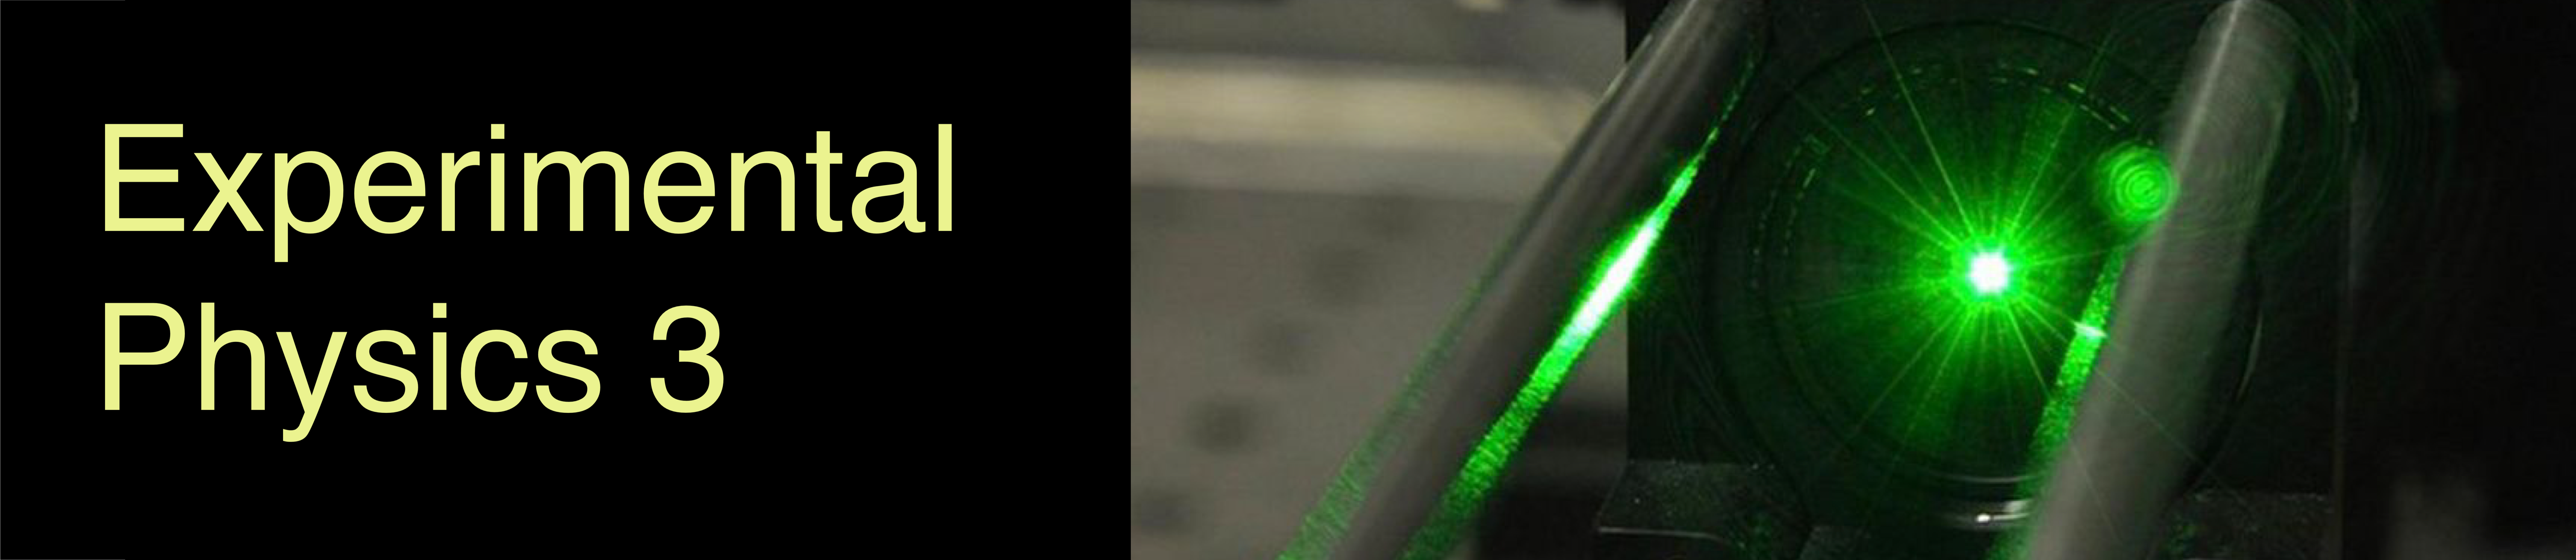
\includegraphics[keepaspectratio]{./assets/images/main/CompSoft_banner.png}}

\bookmarksetup{startatroot}

\chapter{Welcome to the Experimental Physics 3
Course!}\label{welcome-to-the-experimental-physics-3-course}

In this Experimental Physics 3 course, we will explore fundamental
experiments and mathematical descriptions related to light propagation,
electromagnetic waves, and their material counterpart, matter waves.
Specifically, we will focus on:

\begin{itemize}
\tightlist
\item
  Geometrical Optics
\item
  Wave Optics
\item
  Electromagnetic Waves
\item
  Matter Waves and Quantum Mechanics
\end{itemize}

The fields of optics and quantum mechanics are currently vibrant areas
of research, with rapidly evolving optical technologies, high-resolution
microscopy, and quantum information science. All of these advancements
build upon the foundations that we will address in this course.

\section{Course Participation}\label{course-participation}

\begin{figure}

\centering{

\pandocbounded{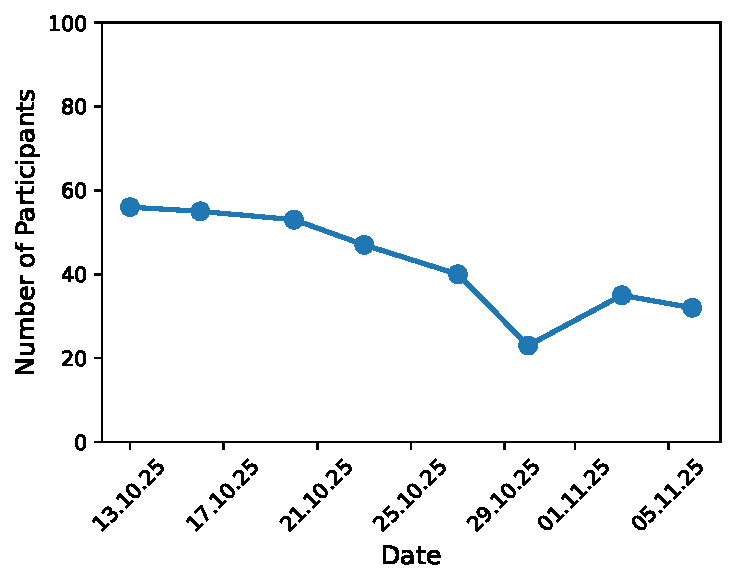
\includegraphics[keepaspectratio]{index_files/figure-pdf/fig-participation-output-1.pdf}}

}

\caption{\label{fig-participation}Number of participants over time in
the lecture. The dashed line indicates the number of course
participants.}

\end{figure}%

\section{Seminar Participation}\label{seminar-participation}

\begin{figure}

\centering{

\pandocbounded{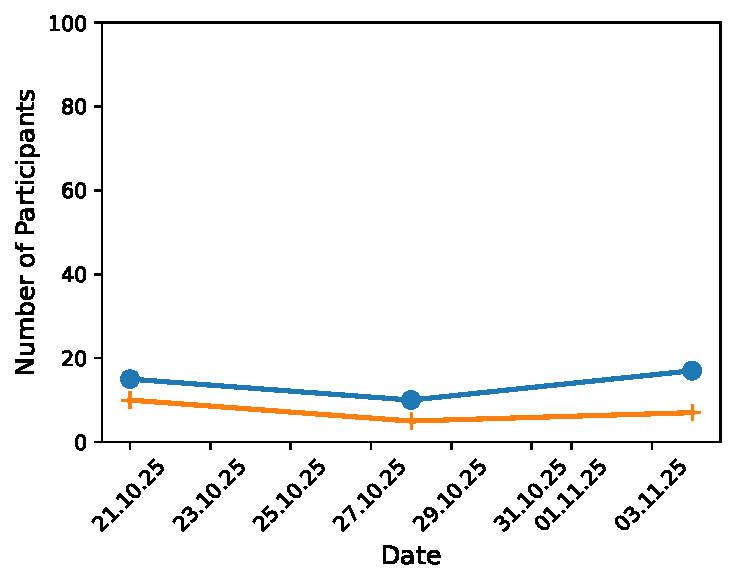
\includegraphics[keepaspectratio]{index_files/figure-pdf/fig-participation_seminar-output-1.pdf}}

}

\caption{\label{fig-participation_seminar}Number of participants over
time in the seminars. The dashed line indicates half the number of
course participants.}

\end{figure}%

\section{Submitted Homeworks}\label{submitted-homeworks}

\begin{figure}

\centering{

\pandocbounded{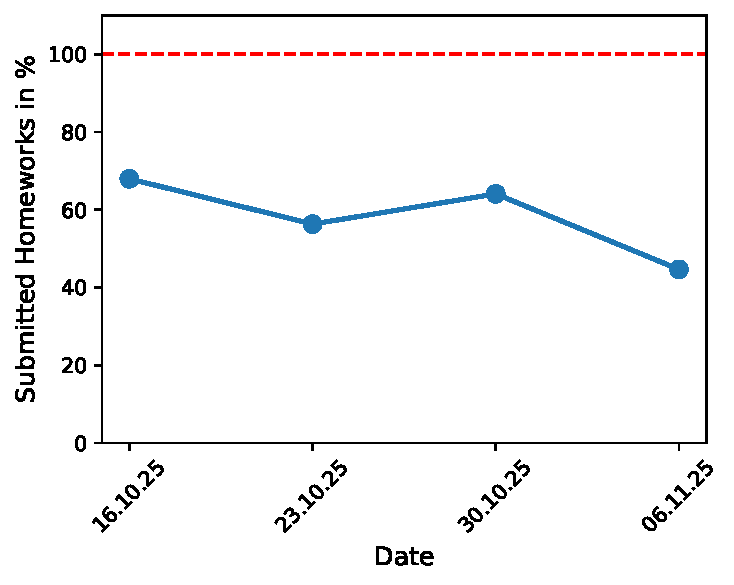
\includegraphics[keepaspectratio]{index_files/figure-pdf/fig-submitted-output-1.pdf}}

}

\caption{\label{fig-submitted}Percentage of submitted homeworks.}

\end{figure}%

\section{Average Points of Total}\label{average-points-of-total}

\begin{figure}

\centering{

\pandocbounded{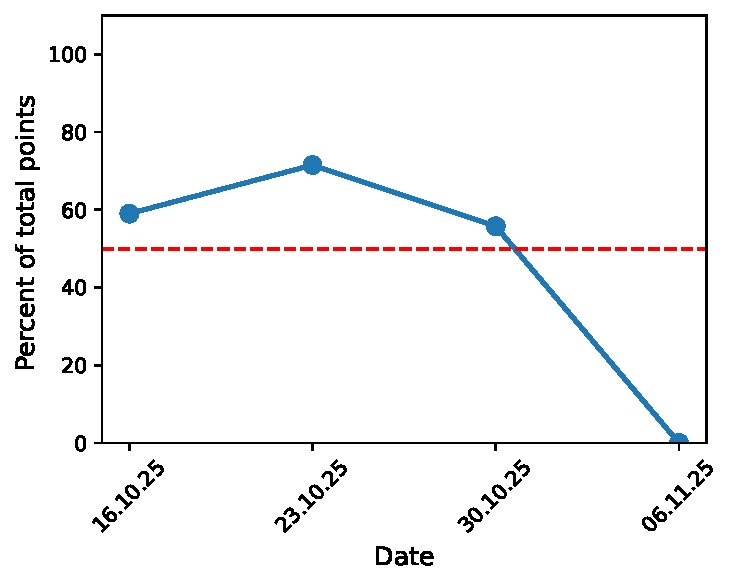
\includegraphics[keepaspectratio]{index_files/figure-pdf/fig-points-output-1.pdf}}

}

\caption{\label{fig-points}Average Percentage of Points of Total
Points.}

\end{figure}%

\section{Homework Statistics}\label{homework-statistics}

\begin{figure}

\centering{

\pandocbounded{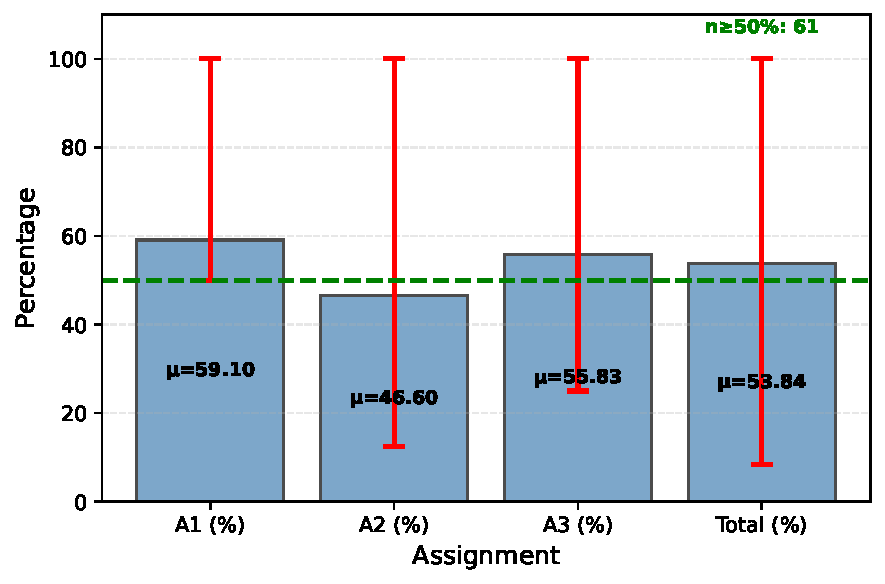
\includegraphics[keepaspectratio]{index_files/figure-pdf/fig-homework-stats-output-1.pdf}}

}

\caption{\label{fig-homework-stats}Statistics for each homework
assignment and total percentage. Bars show mean values, with error bars
indicating min (non-zero) and max values.}

\end{figure}%

\part{Geometrical Optics}

\chapter{Geometrical Optics}\label{geometrical-optics-1}

In this section, we will explore the fundamental principles that govern
how light behaves when it encounters different media and surfaces.

\section{\texorpdfstring{\textbf{Learning
Objectives}}{Learning Objectives}}\label{learning-objectives}

By the end of this section, you should be able to:

\begin{itemize}
\tightlist
\item
  Understand and apply the laws of reflection and refraction.
\item
  Analyze image formation by mirrors, lenses, and prisms.
\item
  Describe the working principles of various optical instruments.
\item
  Explain phenomena such as dispersion and imaging errors.
\end{itemize}

\section{\texorpdfstring{\textbf{Topics
Covered}}{Topics Covered}}\label{topics-covered}

\begin{enumerate}
\def\labelenumi{\arabic{enumi}.}
\item
  \textbf{\href{reflection.qmd}{Reflection}} Explore how light reflects
  off surfaces following the law of reflection.
\item
  \textbf{\href{refraction-total-internal-reflection.qmd}{Refraction and
  Total Internal Reflection}} Understand how light bends when passing
  through different media and the conditions for total internal
  reflection.
\item
  \textbf{\href{Optical\%20Elements\%20I.qmd}{Mirrors},\href{Optical\%20Elements\%20II.qmd}{Prisms}
  and \href{Optical\%20Elements\%20III.qmd}{Lenses} } Learn about
  various optical elements and how they form images.
\item
  \textbf{Optical Instruments} Study devices like telescopes and
  microscopes that utilize mirrors and lenses.
\item
  \textbf{Dispersion} Discover how different wavelengths of light
  refract differently, leading to phenomena like rainbows.
\item
  \textbf{Imaging Errors} Examine common aberrations in optical systems
  and methods to correct them.
\end{enumerate}

\section{\texorpdfstring{\textbf{Introduction}}{Introduction}}\label{introduction}

Geometrical optics is an approximate description of light propagation in
the limit of infinitely small wavelength, where all wave phenomena like
diffraction can be neglected.

\begin{figure}

{\centering 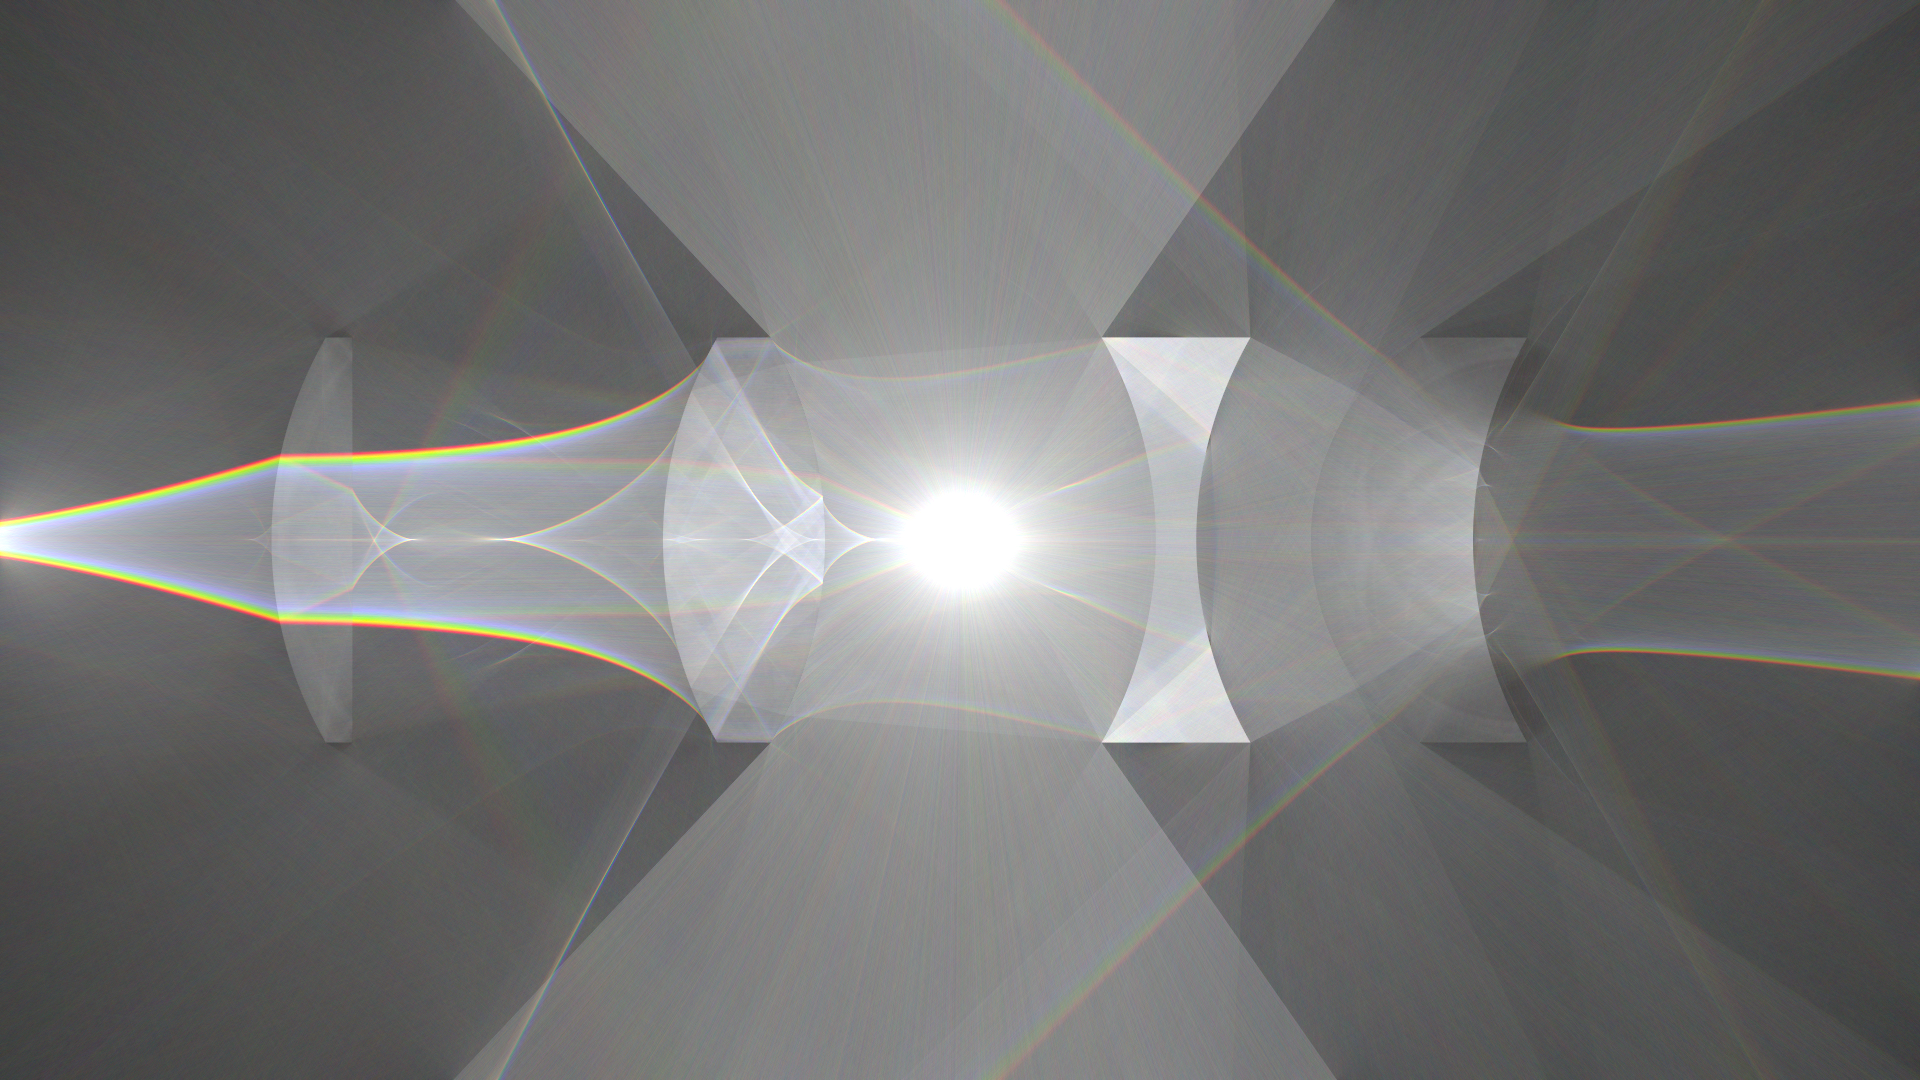
\includegraphics[width=1\linewidth,height=\textheight,keepaspectratio]{geometrical-optics/img/geometrical-optics-intro.png}

}

\caption{Light rays passing through a lens system generated with
\href{https://benedikt-bitterli.me/tantalum/tantalum.html}{Tantalum}}

\end{figure}%

Light interacts with materials in predictable ways, allowing us to
design optical systems for imaging, magnification, and more.

\section{Assumptions of Geometrical
Optics}\label{assumptions-of-geometrical-optics}

Geometrical optics provides an approximate description of light behavior
and is based on several key assumptions. These assumptions simplify the
complex nature of light while still allowing for accurate predictions in
many practical scenarios.

\begin{tcolorbox}[enhanced jigsaw, breakable, toptitle=1mm, bottomrule=.15mm, colbacktitle=quarto-callout-note-color!10!white, title=\textcolor{quarto-callout-note-color}{\faInfo}\hspace{0.5em}{Core Assumptions}, arc=.35mm, rightrule=.15mm, bottomtitle=1mm, opacityback=0, toprule=.15mm, coltitle=black, leftrule=.75mm, opacitybacktitle=0.6, colback=white, left=2mm, titlerule=0mm, colframe=quarto-callout-note-color-frame]

\begin{enumerate}
\def\labelenumi{\arabic{enumi}.}
\tightlist
\item
  \textbf{Light Sources and Detection:}

  \begin{itemize}
  \tightlist
  \item
    Light rays emerge from a light source
  \item
    Light rays are detected by a detector
  \end{itemize}
\item
  \textbf{Light-Matter Interaction:}

  \begin{itemize}
  \tightlist
  \item
    Interaction is characterized by a refractive index \(n\)
  \item
    The speed of light in a medium is given by \(c=c_0/n\), where
    \(c_0\) is the speed of light in vacuum
  \item
    The speed in vacuum is \textbf{299.792.458 m/s} and is connected to
    the definition of the meter
  \end{itemize}
\item
  \textbf{Light Propagation:}

  \begin{itemize}
  \tightlist
  \item
    Light propagates in straight line paths (rays) in a homogeneous
    medium
  \item
    Light bends to a curved path in inhomogeneous media with varying
    refractive index \(n(\textbf{r})\)
  \end{itemize}
\item
  \textbf{Behavior at Interfaces:}

  \begin{itemize}
  \tightlist
  \item
    Rays may be reflected and refracted at interfaces between media
  \end{itemize}
\end{enumerate}

These assumptions form the foundation for understanding and predicting
light behavior in the context of geometrical optics.

\end{tcolorbox}

\chapter{Reflection}\label{reflection}

\begin{tcolorbox}[enhanced jigsaw, breakable, toptitle=1mm, bottomrule=.15mm, colbacktitle=quarto-callout-note-color!10!white, title=\textcolor{quarto-callout-note-color}{\faInfo}\hspace{0.5em}{Historical Context of Reflection Laws}, arc=.35mm, rightrule=.15mm, bottomtitle=1mm, opacityback=0, toprule=.15mm, coltitle=black, leftrule=.75mm, opacitybacktitle=0.6, colback=white, left=2mm, titlerule=0mm, colframe=quarto-callout-note-color-frame]

The study of reflection has a rich history dating back to ancient times:

\begin{enumerate}
\def\labelenumi{\arabic{enumi}.}
\item
  \textbf{Ancient Greece (300 BCE)}: Euclid, in his work ``Catoptrics,''
  was among the first to formally describe the law of reflection. He
  stated that the angle of incidence equals the angle of reflection.
\item
  \textbf{Ancient Rome (50 CE)}: Hero of Alexandria expanded on Euclid's
  work, applying the principle that light travels along the path of
  least distance.
\item
  \textbf{Islamic Golden Age (1000 CE)}: Ibn al-Haytham (Alhazen) made
  significant contributions to optics in his ``Book of Optics.'' He
  conducted experiments to verify the law of reflection and explored the
  properties of spherical and parabolic mirrors.
\item
  \textbf{17th Century}: Fermat's Principle, formulated by Pierre de
  Fermat, provided a more general framework for understanding reflection
  (and refraction) based on the principle of least time.
\end{enumerate}

\textbf{Note}: For reflection in a uniform medium, Hero's principle of
least distance is mathematically equivalent to Fermat's principle of
least time, since distance and time are proportional when the speed of
light is constant (\(t = l/c\)). However, Fermat's formulation is more
general and applies to refraction as well, where light travels at
different speeds in different media.

\begin{enumerate}
\def\labelenumi{\arabic{enumi}.}
\setcounter{enumi}{4}
\tightlist
\item
  \textbf{Modern Era}: The understanding of reflection has been further
  refined with the development of electromagnetic theory by James Clerk
  Maxwell in the 19th century and quantum optics in the 20th century.
\end{enumerate}

\end{tcolorbox}

The law of reflection is probably the most simple one. Yet the
simplicity gives us the chance to define some basic objects which we
will further use for the description of light rays and their
propagation.

\subsection{Law of Reflection}\label{sec-law-of-reflection}

The sketch below shows the reflection of an incoming light ray (red) on
an interface. This incoming light ray has an angle \(\theta_{1}\) with
the axis (dashed line), which is perpendicular to the reflecting
surface. As compared to X-ray diffraction, we measure the angle to the
normal of the surface and not to the surface itself.

\begin{figure}

\begin{minipage}{0.50\linewidth}

\centering{

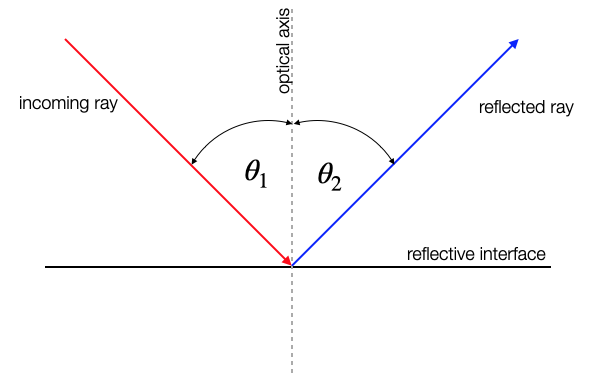
\includegraphics[width=0.8\linewidth,height=\textheight,keepaspectratio]{geometrical-optics/../assets/images/reflection/reflection.png}

}

\subcaption{\label{fig-reflection-diagram}Law of reflection}

\end{minipage}%
%
\begin{minipage}{0.50\linewidth}

\centering{

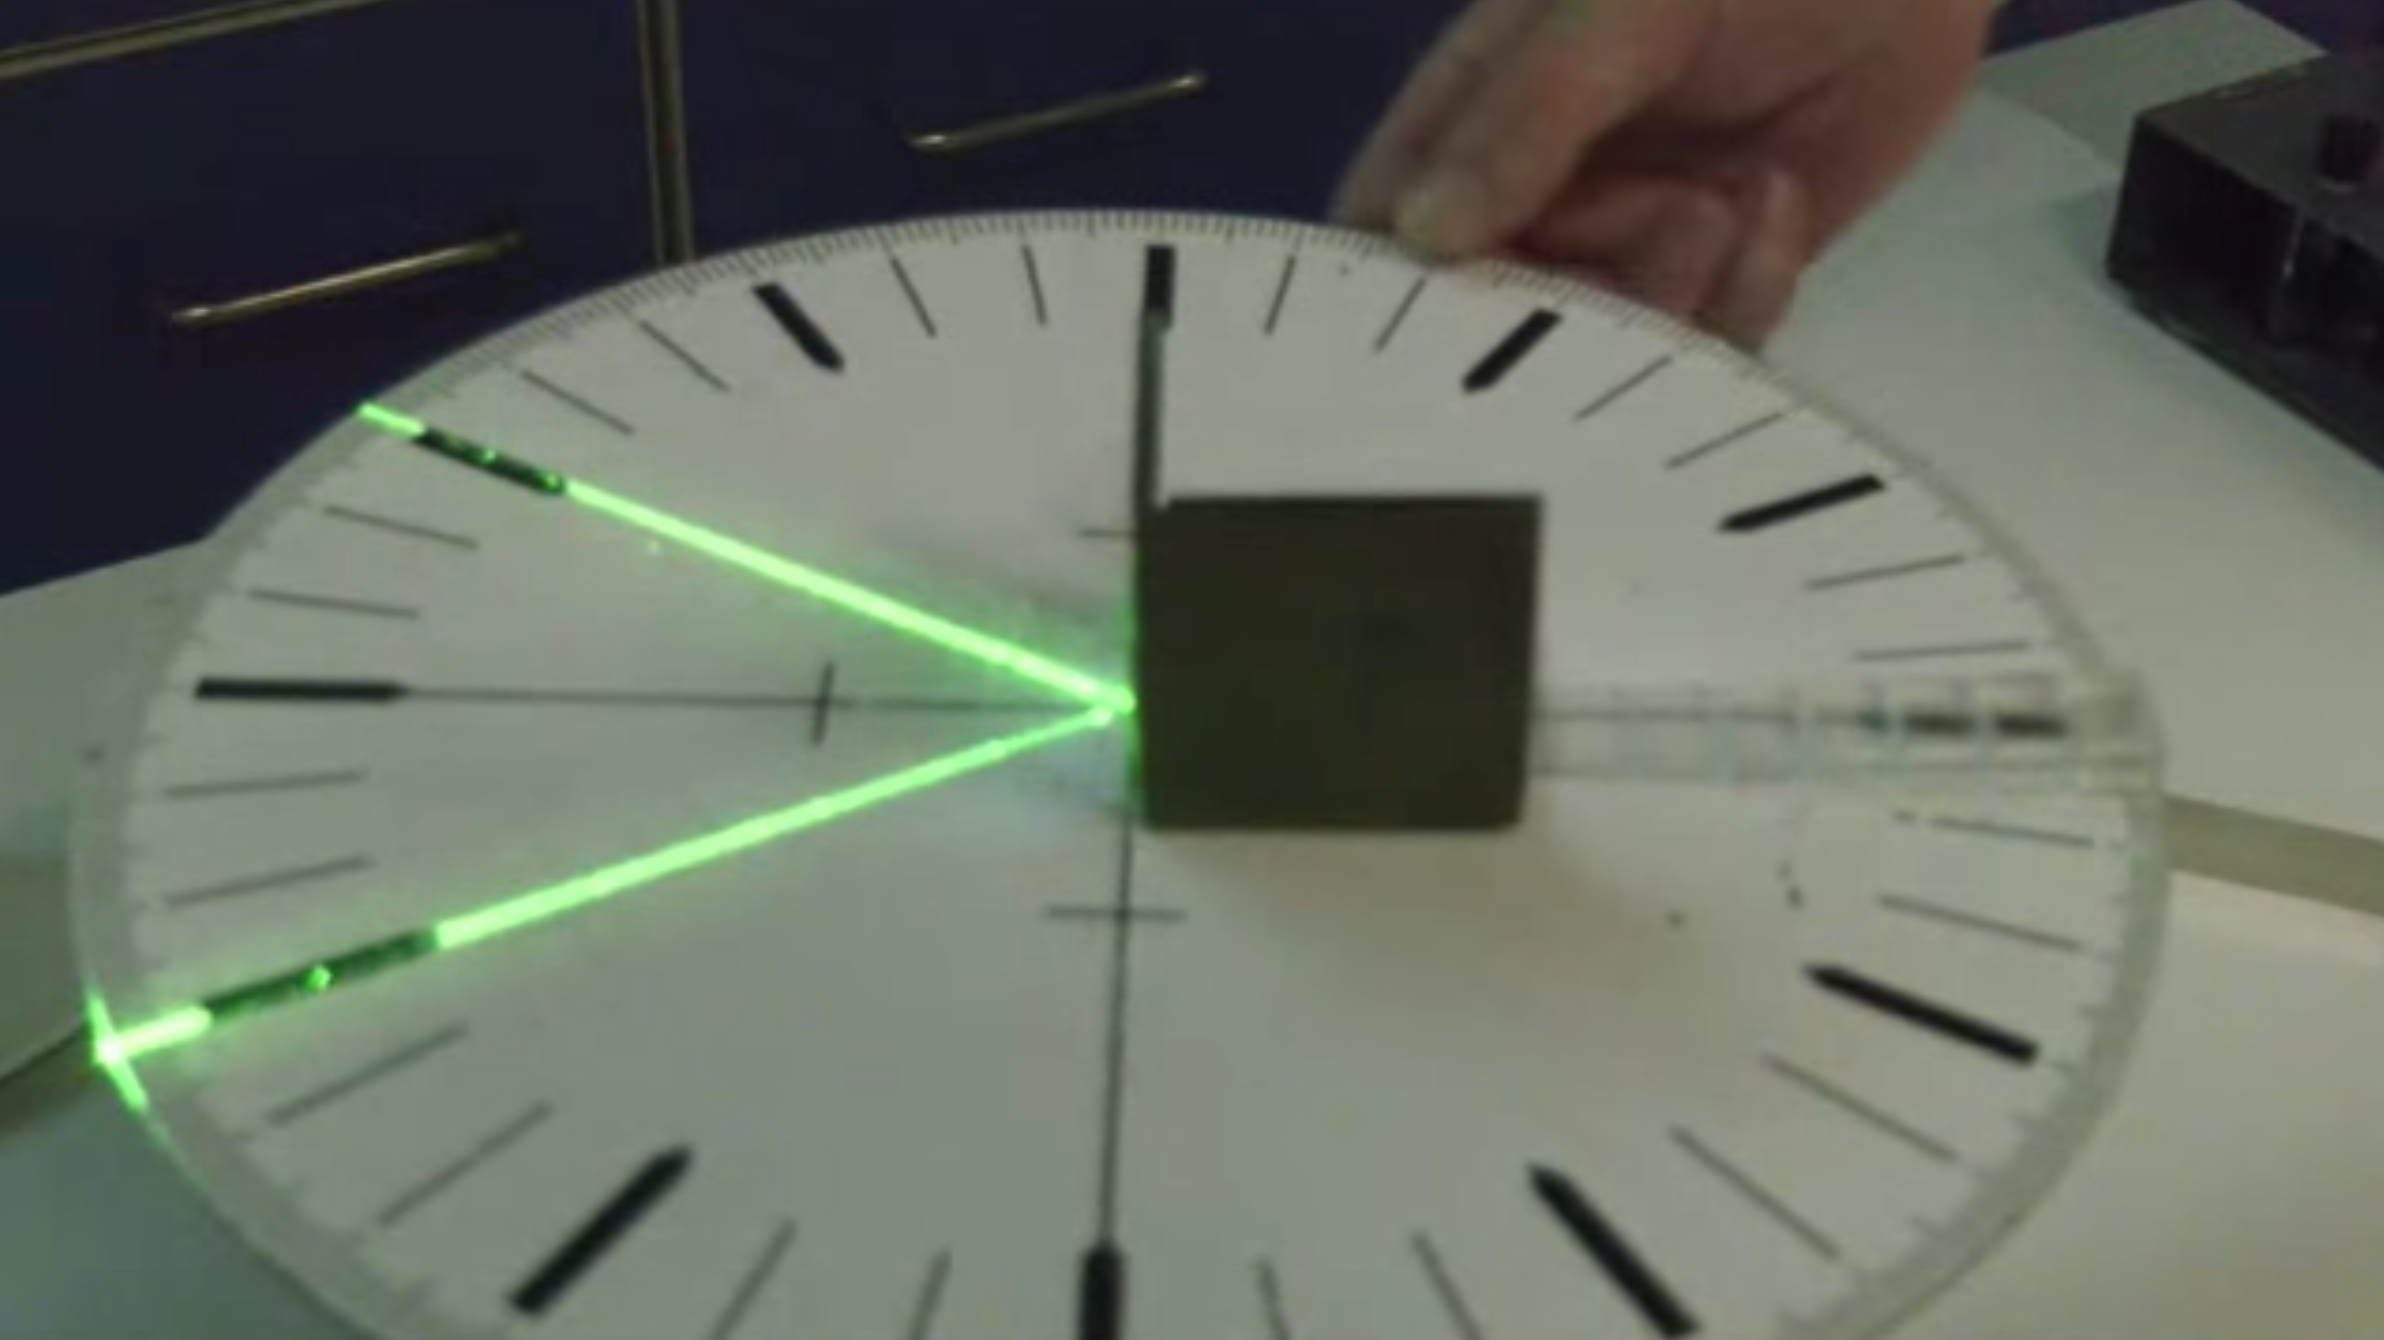
\includegraphics[width=0.8\linewidth,height=\textheight,keepaspectratio]{geometrical-optics/../assets/images/reflection/reflection_law.png}

}

\subcaption{\label{fig-reflection-experiment}Experimental Demonstration}

\end{minipage}%

\caption{\label{fig-reflection}Figure~\ref{fig-reflection-diagram}
illustrates the law of reflection, while Figure
Figure~\ref{fig-reflection-experiment} shows an experimental
demonstration.}

\end{figure}%

Figure~\ref{fig-reflection-diagram} shows the reflection of an incoming
light ray (red) on an interface. This incoming light ray has an angle
\(\theta_{1}\) with the axis (dashed line), which is perpendicular to
the reflecting surface. As compared to X-ray diffraction, we measure the
angle to the normal of the surface and not to the surface itself.

The law of reflection tells us now, that the outgoing reflected ray is
now leaving the surface under an angle \(\theta_2=\theta_1\). So both
angles are the same for the reflection.

\begin{tcolorbox}[enhanced jigsaw, breakable, toptitle=1mm, bottomrule=.15mm, colbacktitle=quarto-callout-tip-color!10!white, title=\textcolor{quarto-callout-tip-color}{\faLightbulb}\hspace{0.5em}{Law of Reflection}, arc=.35mm, rightrule=.15mm, bottomtitle=1mm, opacityback=0, toprule=.15mm, coltitle=black, leftrule=.75mm, opacitybacktitle=0.6, colback=white, left=2mm, titlerule=0mm, colframe=quarto-callout-tip-color-frame]

If a ray is incident to a reflecting surface under an angle \(\theta_1\)
it will be reflected towards under an angle \(\theta_2=\theta_1\) to the
same side of the surface.

\end{tcolorbox}

\subsection{Fermat's Principle}\label{sec-fermat-principle}

The law of reflection can be actually obtained from a variational
principle saying the light rays propagate along those path on which the
propagation time is an extremum. This variational principle is called
Fermat's principle.

\begin{figure}

\centering{

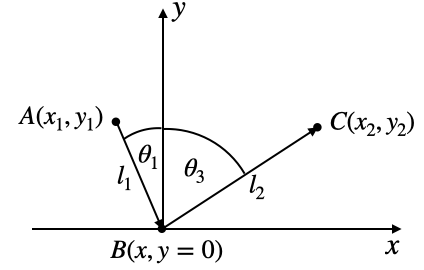
\includegraphics[width=0.6\linewidth,height=\textheight,keepaspectratio]{geometrical-optics/../assets/images/reflection/fermat.png}

}

\caption{\label{fig-fermat}Sketch for deriving the law of reflection
from Fermat's principle}

\end{figure}%

Consider now a light ray that should travel from point \(A\) to point
\(C\) via a point \(B\) on the mirror surface. In general multiple paths
are possible such as the one indicated in the above picture. Clearly
this path is not satisfying our reflection law formulated above.
Fermat's principle now restricts the path length from \(A\) to \(C\) to
be the one, which takes the least amount of time.

\begin{tcolorbox}[enhanced jigsaw, breakable, toptitle=1mm, bottomrule=.15mm, colbacktitle=quarto-callout-tip-color!10!white, title=\textcolor{quarto-callout-tip-color}{\faLightbulb}\hspace{0.5em}{Fermat's principle}, arc=.35mm, rightrule=.15mm, bottomtitle=1mm, opacityback=0, toprule=.15mm, coltitle=black, leftrule=.75mm, opacitybacktitle=0.6, colback=white, left=2mm, titlerule=0mm, colframe=quarto-callout-tip-color-frame]

The path taken by a ray between two given points A, B is the path that
can be traversed in the least time.

\emph{More precise alternative:} A ray going in a certain particular
path has the property that if we make a small change in the ray in any
manner whatever, say in the location at which it comes to the mirror, or
the shape of the curve, or anything, there will be no first-order change
in the time; there will be only a second-order change in the time.

\end{tcolorbox}

So let us consider that contraints to the path length. The total length
the light has to travel via the three points is

\[
l=l_{1}+l_{2}=\sqrt{(x-x_1)^2+y_1^2}+\sqrt{(x_2-x)^2+y_2^2}
\]

The time that is required by the light to travel that distance \(l\) is
then given by

\[
t=\frac{l}{c},
\]

where \(c\) is the speed of light in the medium above the mirror. If
this time should now be a minimum, we have to take the derivative of the
time \(t\) with respect to the position \(x\) on the mirror and set that
to zero, i.e.,

\[\frac{\mathrm dt}{\mathrm dx}=0.\]

Let's visualize how the path length \(l\) varies as we change the
position \(x\) on the mirror:

\begin{figure}

\centering{

\pandocbounded{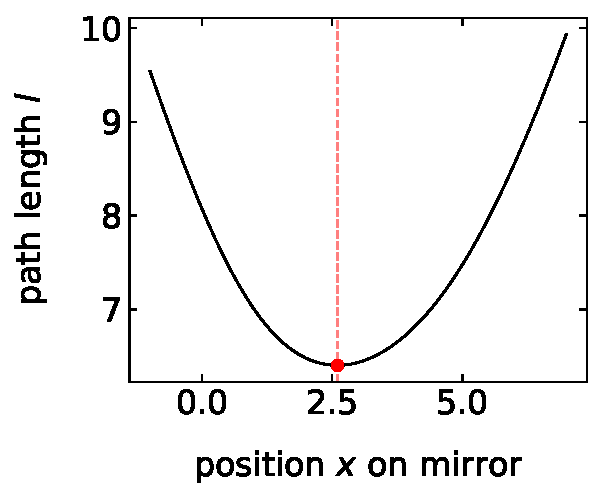
\includegraphics[keepaspectratio]{geometrical-optics/reflection_files/figure-pdf/fig-planar-reflection-output-1.pdf}}

}

\caption{\label{fig-planar-reflection}Total optical pathlength upon
reflection of a ray on a planar mirror indicating the second order
change with a minimum.}

\end{figure}%

As we can see from the plot, the path length has a clear minimum at a
specific position on the mirror. This minimum corresponds to the point
where the angle of incidence equals the angle of reflection, confirming
the law of reflection through Fermat's principle.

Taking the derivative of the time with respect to \(x\) corresponds to
taking the derivative of the path length with respect to \(x\) and
setting it equal to zero for the minimum:

\[
\frac{\mathrm dl}{\mathrm dx} = \frac{x-x_1}{\sqrt{(x-x_1)^2+y_1^2}} - \frac{x_2-x}{\sqrt{(x_2-x)^2+y_2^2}} = 0
\]

This gives us:

\begin{equation}\phantomsection\label{eq-hello}{
\frac{x-x_1}{\sqrt{(x-x_1)^2+y_{1}^2}}=\frac{x_2-x}{\sqrt{(x_2-x)^2+y_{2}^2}},
}\end{equation}

which simplifies to:

\[
\frac{x-x_1}{l_1}=\frac{x_2-x}{l_2}
\]

Looking at the geometry in Figure~\ref{fig-fermat}, we can identify
these ratios as the sines of the respective angles:
\((x-x_1)/l_1 = \sin(\theta_1)\) and \((x_2-x)/l_2 = \sin(\theta_2)\).
Therefore, Equation~\ref{eq-hello} becomes:

\[
\sin(\theta_1)=\sin(\theta_2)
\]

which requires:

\[
\theta_1=\theta_2
\]

This is our law of reflection. Thus, reflection satisfies Fermat's
principle---the light rays propagate along those paths on which the
propagation time is an extremum.

\begin{tcolorbox}[enhanced jigsaw, breakable, toptitle=1mm, bottomrule=.15mm, colbacktitle=quarto-callout-tip-color!10!white, title=\textcolor{quarto-callout-tip-color}{\faLightbulb}\hspace{0.5em}{Principle of Least Action (Hamilton's Principle)}, arc=.35mm, rightrule=.15mm, bottomtitle=1mm, opacityback=0, toprule=.15mm, coltitle=black, leftrule=.75mm, opacitybacktitle=0.6, colback=white, left=2mm, titlerule=0mm, colframe=quarto-callout-tip-color-frame]

The Principle of Least Action, also known as Hamilton's Principle, is a
fundamental concept in classical mechanics. It states that the path
taken by a physical system between two states is the one for which the
action integral is stationary (usually a minimum).

\subsection{Action Integral}\label{action-integral}

The action \(S\) is defined as the integral of the Lagrangian \(L\) over
time:

\[
S = \int_{t_1}^{t_2} L \, dt
\]

\subsection{Lagrangian}\label{lagrangian}

The Lagrangian \(L\) is a function that summarizes the dynamics of the
system. For a system with generalized coordinates \(q_i\) and velocities
\(\dot{q}_i\), the Lagrangian is typically given by:

\[
L = T - V
\]

where:

\begin{itemize}
\item
  \(T\) is the kinetic energy of the system.
\item
  \(V\) is the potential energy of the system.
\end{itemize}

\subsection{Euler-Lagrange Equations}\label{euler-lagrange-equations}

Hamilton's Principle leads to the Euler-Lagrange equations, which are
the equations of motion for the system. These equations are derived by
requiring that the action \(S\) be stationary with respect to variations
in the path \(q_i(t)\):

\[
\delta S = 0
\]

This condition leads to the following differential equations:

\[
\frac{d}{dt} \left( \frac{\partial L}{\partial \dot{q}_i} \right) - \frac{\partial L}{\partial q_i} = 0
\]

These are the Euler-Lagrange equations, and they provide a powerful
method for deriving the equations of motion for a wide variety of
physical systems.

\subsection{Example: Simple Harmonic
Oscillator}\label{example-simple-harmonic-oscillator}

For a simple harmonic oscillator with mass \(m\) and spring constant
\(k\), the Lagrangian is:

\[
L = \frac{1}{2} m \dot{x}^2 - \frac{1}{2} k x^2
\]

Applying the Euler-Lagrange equation:

\[
\frac{d}{dt} \left( \frac{\partial L}{\partial \dot{x}} \right) - \frac{\partial L}{\partial x} = 0
\]

we get:

\[
m \ddot{x} + k x = 0
\]

which is the familiar equation of motion for a simple harmonic
oscillator.

Hamilton's Principle and the associated Euler-Lagrange equations are
foundational in classical mechanics and have far-reaching implications
in other areas of physics, including quantum mechanics and field theory.

\end{tcolorbox}

\chapter{Refraction and Total Internal
Reflection}\label{refraction-and-total-internal-reflection}

\section{Refraction}\label{refraction}

\begin{tcolorbox}[enhanced jigsaw, breakable, toptitle=1mm, bottomrule=.15mm, colbacktitle=quarto-callout-note-color!10!white, title=\textcolor{quarto-callout-note-color}{\faInfo}\hspace{0.5em}{Historical Context of Refraction}, arc=.35mm, rightrule=.15mm, bottomtitle=1mm, opacityback=0, toprule=.15mm, coltitle=black, leftrule=.75mm, opacitybacktitle=0.6, colback=white, left=2mm, titlerule=0mm, colframe=quarto-callout-note-color-frame]

The understanding of refraction has evolved over centuries, with
contributions from various cultures and scientific traditions. This
timeline highlights key milestones in the discovery and formalization of
refraction, showcasing how our comprehension of this fundamental optical
phenomenon has deepened over time:

\begin{enumerate}
\def\labelenumi{\arabic{enumi}.}
\item
  \textbf{Ancient Greece (3rd century BCE):} Euclid noticed that a stick
  partially submerged in water appears bent. Archimedes studied the
  refraction of light in water.
\item
  \textbf{Ancient Rome (1st century CE):} Ptolemy conducted experiments
  on refraction and compiled tables of refraction angles for different
  media.
\item
  \textbf{Islamic Golden Age (10th-11th centuries):} Ibn Sahl
  (c.~940-1000) used geometric principles related to refraction in his
  work on burning mirrors and lenses, employing techniques that
  anticipated aspects of Snell's law, though the exact nature of his
  formulation remains debated by historians. Alhazen (965-1040) studied
  lenses and the human eye, contributing significantly to optics.
\item
  \textbf{Middle Ages:} Robert Grosseteste (1175-1253) and Roger Bacon
  (1214-1294) studied refraction and its application to lenses.
\item
  \textbf{Renaissance:} Thomas Harriot (c.~1560-1621) experimentally
  investigated refraction around 1602 and found numerical relationships
  between angles, though his work remained unpublished in manuscripts.
\item
  \textbf{17th Century:} Willebrord Snellius (1580-1626) derived the
  mathematical law of refraction (Snell's law) around 1621, though his
  work remained unpublished. René Descartes (1596-1650) independently
  derived and published the law of refraction in his ``Dioptrique''
  (1637). Isaac Newton (1642-1727) conducted extensive experiments with
  prisms and developed his corpuscular theory of light. Pierre de Fermat
  (1607-1665) derived the law of refraction using his principle of least
  time in the 1650s-1660s.
\item
  \textbf{19th Century:} Augustin-Jean Fresnel (1788-1827) developed the
  wave theory of light, explaining refraction in terms of changes in
  wave speed.
\item
  \textbf{20th Century:} The development of quantum mechanics in the
  early 20th century, beginning with Max Planck's work on black body
  radiation (1900) and Albert Einstein's explanation of the
  photoelectric effect (1905), revealed the dual wave-particle nature of
  light. However, for refraction itself, the classical electromagnetic
  wave theory developed by Maxwell remains the primary and most
  practical description. The refractive index arises from the collective
  electromagnetic response of atoms in a material, and while quantum
  mechanics provides a deeper understanding of atomic structure and
  light-matter interactions at the microscopic level, the macroscopic
  phenomenon of refraction is well-described by wave optics.
\end{enumerate}

\end{tcolorbox}

The law of refraction is the second important law of geometrical optics.
It relates the refractive index \(n_1\) and angle of incidence
\(\theta_1\) on one side of an interface to the refractive index \(n_2\)
and angle of refraction \(\theta_2\) on the other side. Both the law of
reflection and the law of refraction can be derived from more
fundamental principles such as Fermat's principle of least time and are
consistent with the conservation of energy. Their relation to momentum
is more complex and involves considering the interaction of light with
the medium at an atomic level. These laws provide a mathematical
framework for predicting how light behaves when it encounters interfaces
between different media, forming the basis for understanding a wide
range of optical phenomena and the design of optical devices.

\subsection{Refractive Index}\label{refractive-index}

The refractive index \(n\) is a material constant representing the
factor by which the speed of light is reduced in the medium compared to
its speed in vacuum. For most natural materials and visible light, the
refractive index is \(n \ge 1\), as light typically travels slower in
media than in vacuum. However, in certain special cases---such as for
X-rays in some materials or in engineered metamaterials---the refractive
index can be less than 1 or even negative. Understanding these exotic
cases requires a deeper exploration of the electromagnetic properties of
materials and the origin of the refractive index, which we will address
later.

\subsection{Snells Law}\label{snells-law}

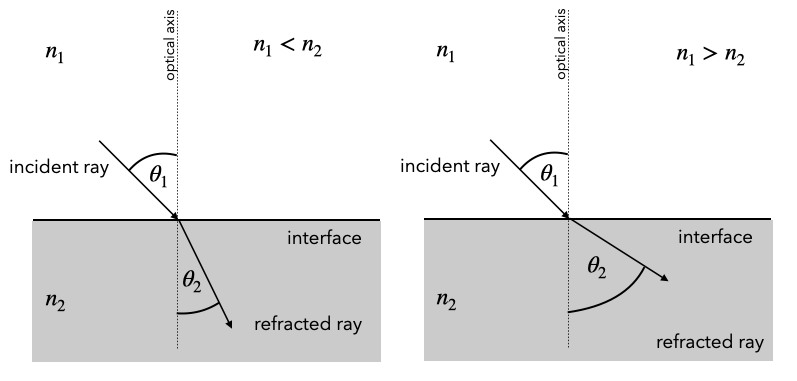
\includegraphics[width=0.59\linewidth,height=\textheight,keepaspectratio]{geometrical-optics/../assets/images/reflection/snell.png}
\begin{center}
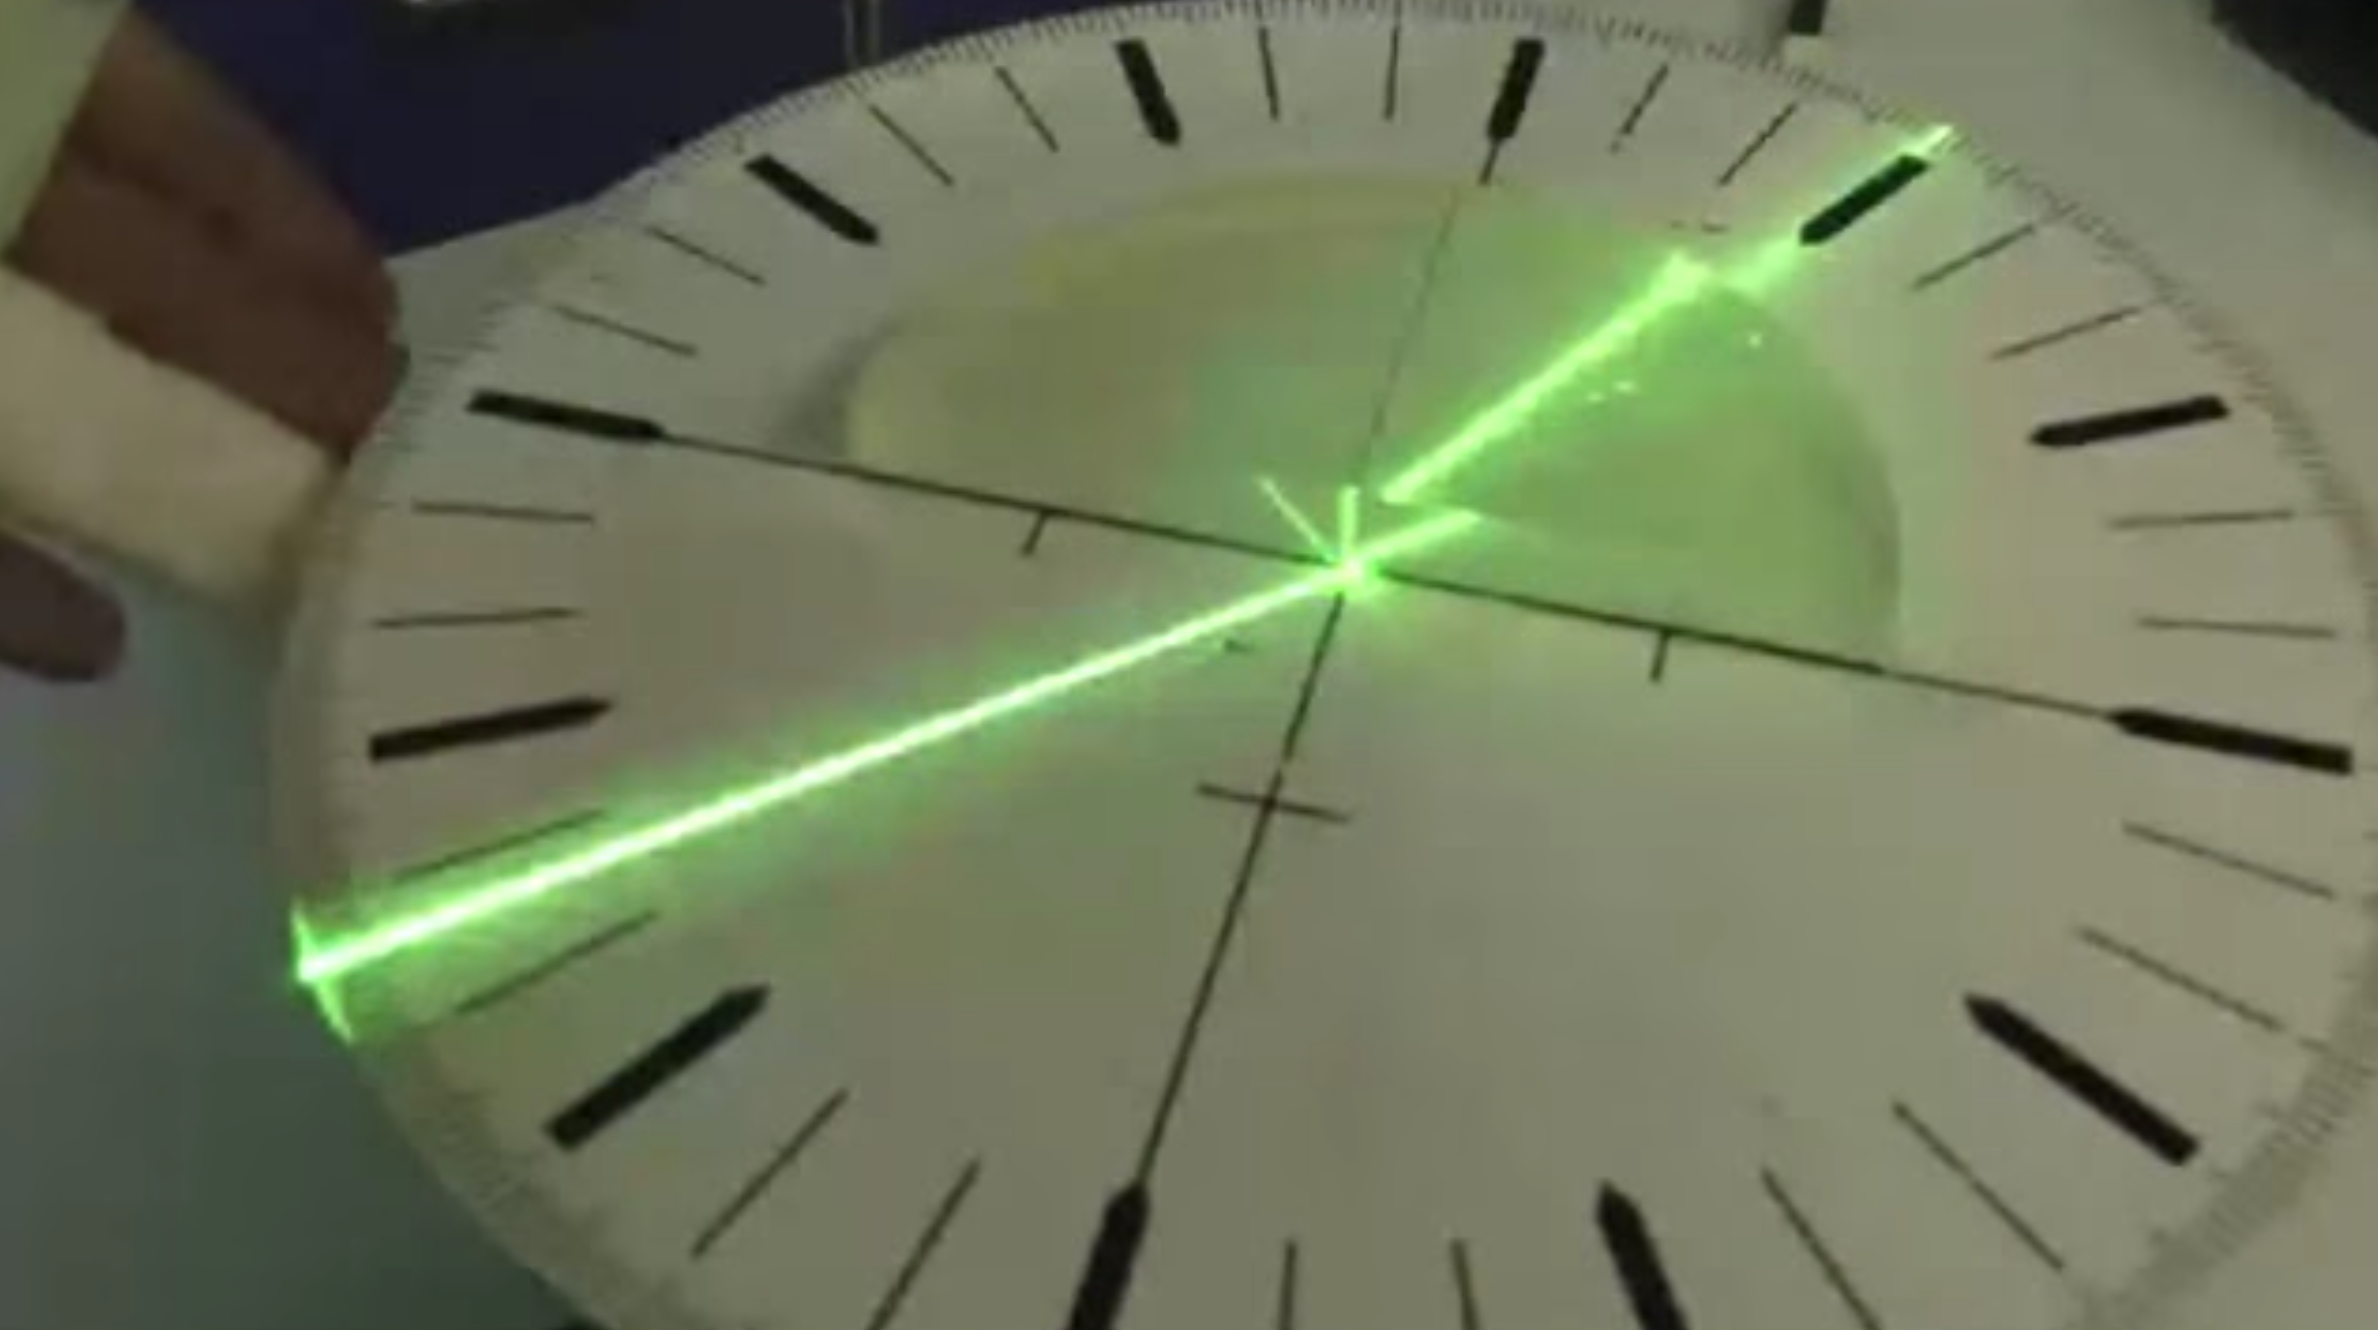
\includegraphics[width=0.4\linewidth,height=\textheight,keepaspectratio]{geometrical-optics/../assets/images/reflection/refraction_law.png}
\end{center}

\begin{tcolorbox}[enhanced jigsaw, breakable, toptitle=1mm, bottomrule=.15mm, colbacktitle=quarto-callout-tip-color!10!white, title=\textcolor{quarto-callout-tip-color}{\faLightbulb}\hspace{0.5em}{Law of Refraction (Snell's Law)}, arc=.35mm, rightrule=.15mm, bottomtitle=1mm, opacityback=0, toprule=.15mm, coltitle=black, leftrule=.75mm, opacitybacktitle=0.6, colback=white, left=2mm, titlerule=0mm, colframe=quarto-callout-tip-color-frame]

The law of refraction (Snell's law) is given for the above sketch by the
equation:

\[
n_1 \sin(\theta_1)=n_2 \sin(\theta_2)
\]

\end{tcolorbox}

You can explore the law of refraction using the interactive
visualization below. The visualization shows a light ray incident on an
interface between two media with different refractive indices. You can
adjust the angle of incidence and the refractive index of the first
medium to see how the angle of refraction changes according to Snell's
law.

Snell's law leads to some general patterns in the behavior of light rays
at interfaces, which are worth remembering. Consider these two cases:

\begin{enumerate}
\def\labelenumi{\arabic{enumi}.}
\tightlist
\item
  When light moves from a medium with lower refractive index to one with
  higher refractive index (\(n_1 < n_2\)):

  \begin{itemize}
  \tightlist
  \item
    The refracted ray bends towards the normal (optical axis)
  \item
    The angle of refraction is smaller than the angle of incidence
    (\(\theta_2 < \theta_1\))
  \end{itemize}
\item
  When light moves from a medium with higher refractive index to one
  with lower refractive index (\(n_1 > n_2\)):

  \begin{itemize}
  \tightlist
  \item
    The refracted ray bends away from the normal (optical axis)
  \item
    The angle of refraction is larger than the angle of incidence
    (\(\theta_2 > \theta_1\))
  \end{itemize}
\end{enumerate}

Figure Figure~\ref{fig-snells-combinations} illustrates these principles
with three plots showing how the refracted angle changes with the
incident angle for two common interface scenarios: glass-to-air and
air-to-glass. These plots clearly demonstrate the different behaviors
described above.

\begin{figure}

\centering{

\pandocbounded{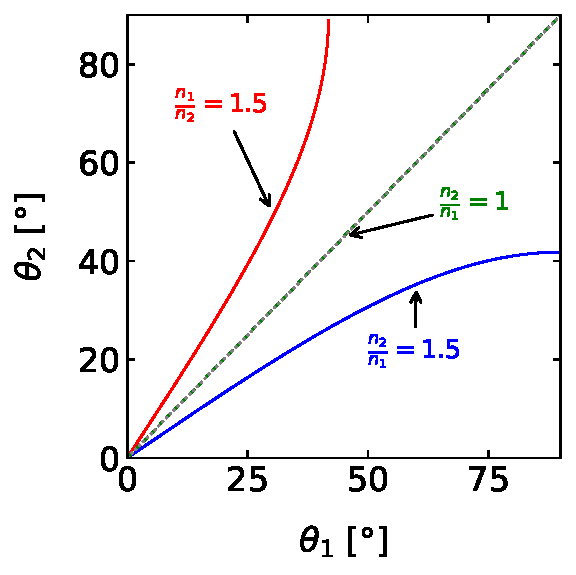
\includegraphics[keepaspectratio]{geometrical-optics/refraction-total-internal-reflection_files/figure-pdf/fig-snells-combinations-output-1.pdf}}

}

\caption{\label{fig-snells-combinations}Snell's law for different
combinations of refractive indices. The plots show the relationship
between incident angle (\(\theta_1\)) and refracted angle (\(\theta_2\))
for three scenarios: (a) light passing from air to glass, (b) light
passing from glass to air, and (c) a comparison of both cases. Note how
the curves differ when light moves into a medium with higher refractive
index versus a lower refractive index.}

\end{figure}%

\subsection{Total Internal Reflection}\label{total-internal-reflection}

The above diagram reveals a special case occurring when \(n_1 > n_2\).
Under these conditions, we can increase the incident angle \(\theta_1\)
until the outgoing angle reaches \(\theta_2 = \frac{\pi}{2}\). At this
point, the refracted ray would be traveling along the interface between
the two media. For any incident angle \(\theta_1\) larger than this
critical angle, there is no refracted ray at all; instead, we observe
only a reflected ray. This phenomenon, known as \textbf{total internal
reflection}, occurs despite the fact that the material with refractive
index \(n_2\) is completely transparent.

Let's formalize this concept mathematically. Using Snell's law and
setting \(\theta_2 = \frac{\pi}{2}\), we obtain the equation for the
critical angle \(\theta_c\):

\[\theta_1 = \theta_c = \sin^{-1}\left(\frac{n_2}{n_1}\right)\]

Note that the \(\sin^{-1}()\) function requires an argument \(\le 1\),
which is why this phenomenon only occurs when \(n_2 < n_1\).

It's important to understand that during total internal reflection, all
of the light energy is reflected back into the first medium, hence the
term `total'. However, electromagnetic optics reveals an interesting
subtlety: an evanescent wave penetrates a short distance into the second
medium, though it doesn't propagate energy across the boundary.

When the incident angle exceeds the critical angle, Snell's law as we've
written it no longer applies. Instead, we observe perfect reflection,
where the angle of reflection equals the angle of incidence, just as in
regular reflection from a mirror. This reflection occurs without any
loss of energy to the second medium, making it an extremely efficient
process.

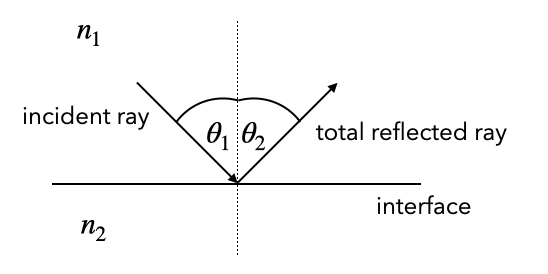
\includegraphics[width=0.5\linewidth,height=\textheight,keepaspectratio]{geometrical-optics/../assets/images/reflection/tir.png}
\begin{center}
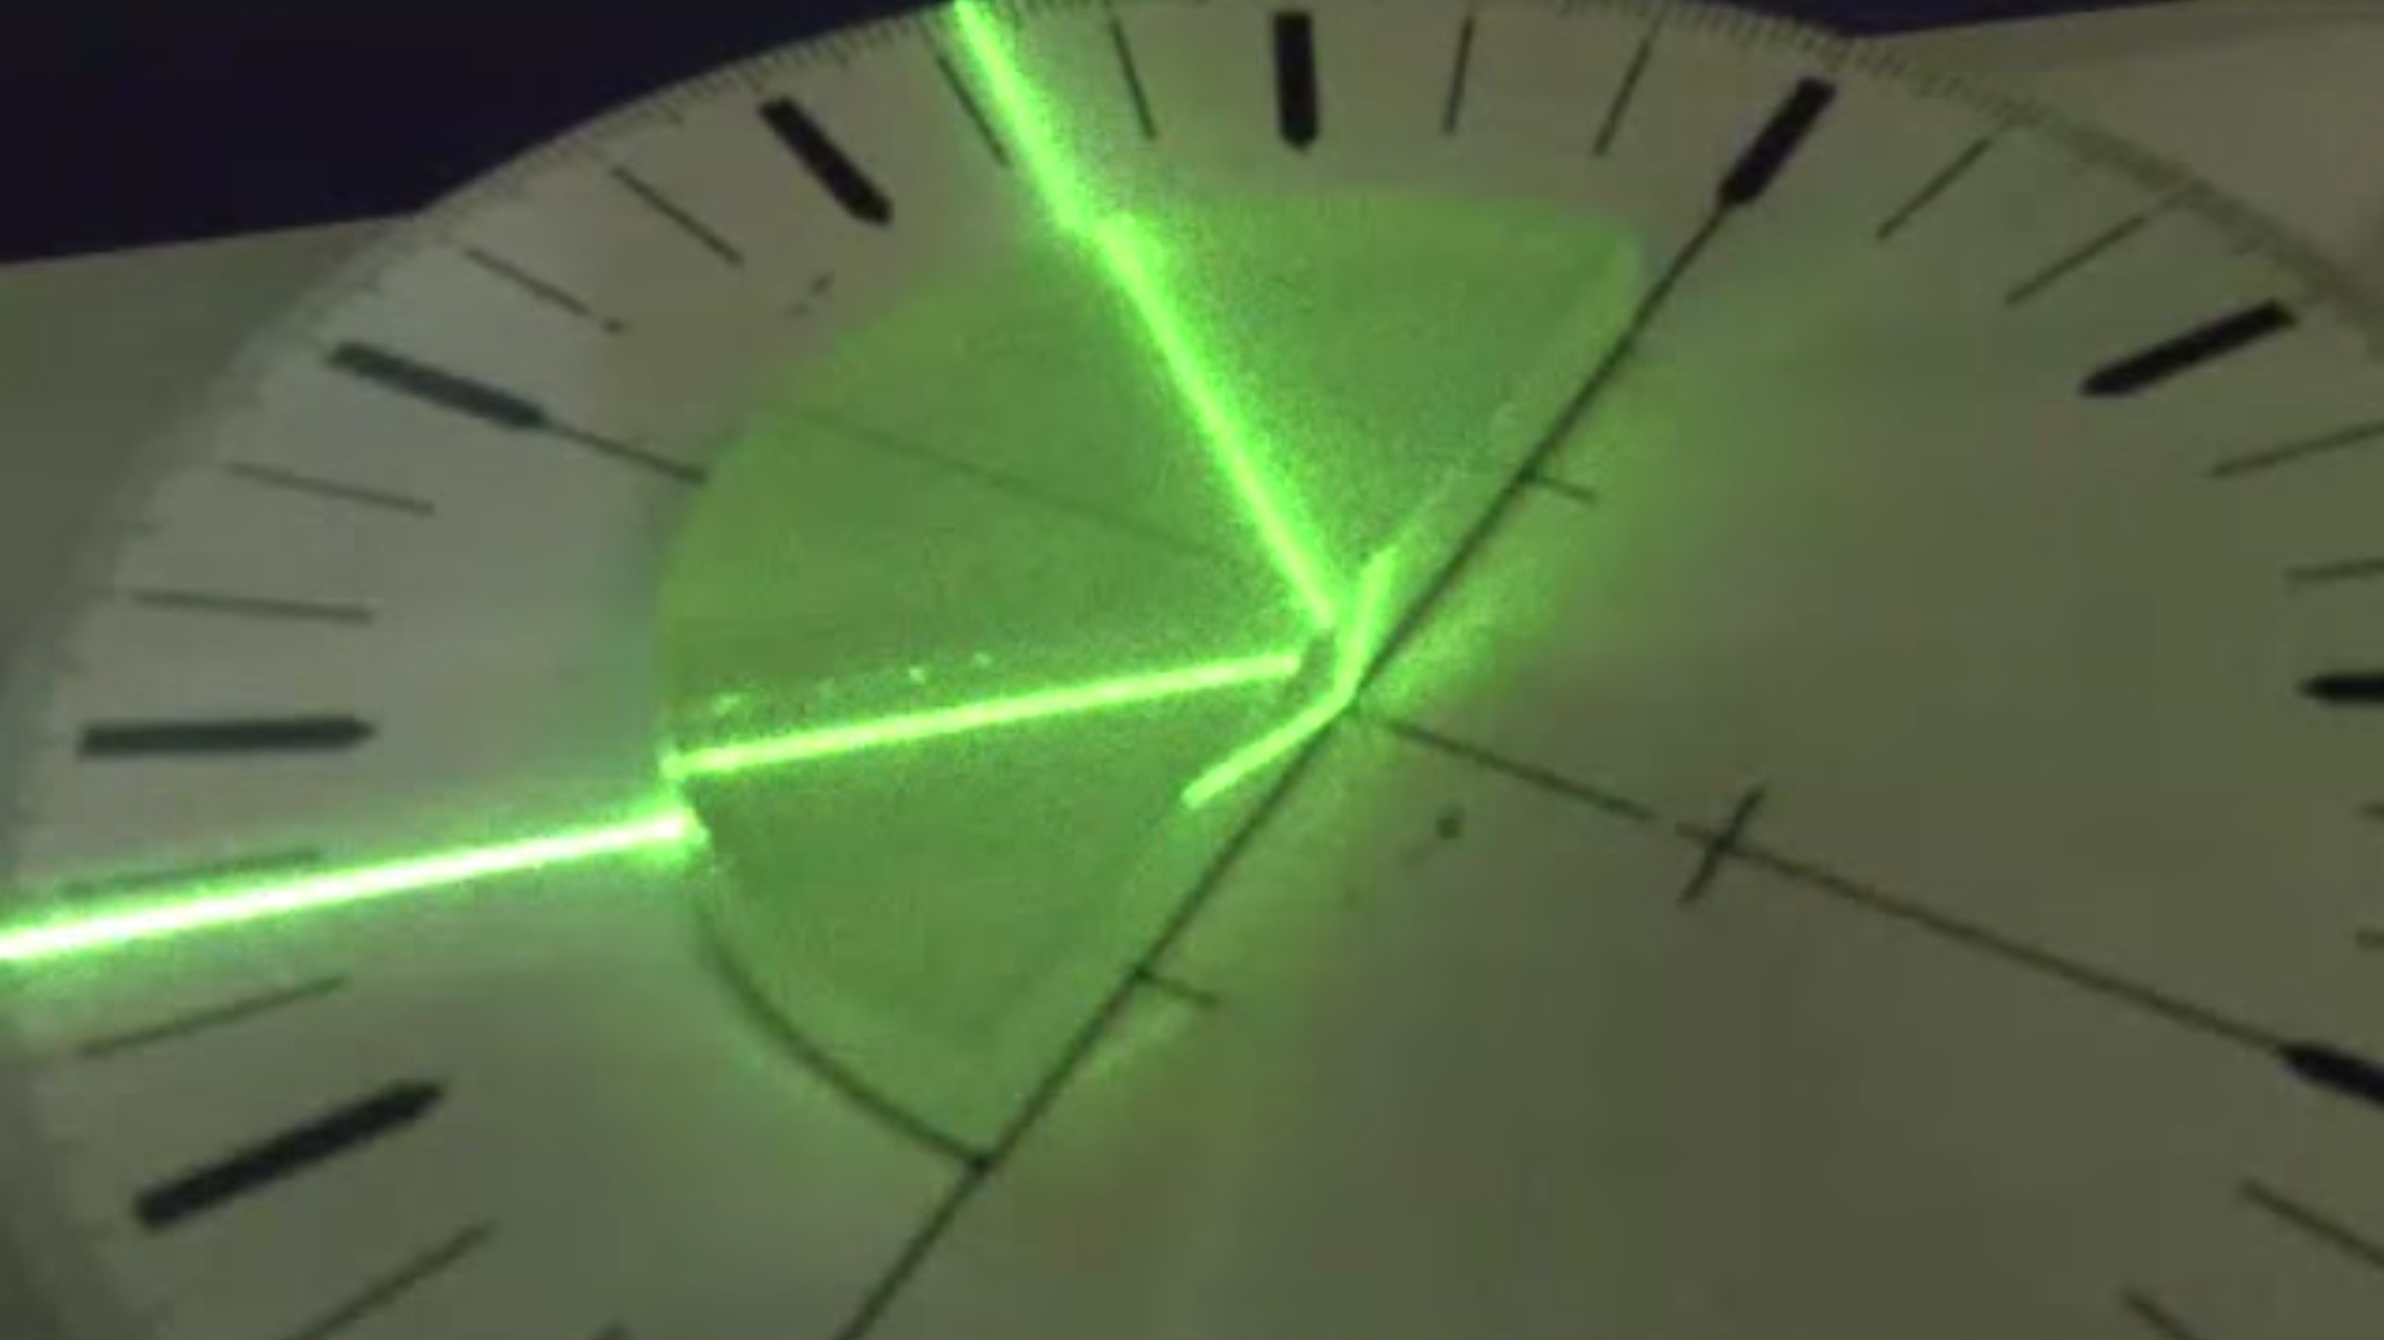
\includegraphics[width=0.49\linewidth,height=\textheight,keepaspectratio]{geometrical-optics/../assets/images/reflection/tir_disk.png}
\end{center}

\begin{tcolorbox}[enhanced jigsaw, breakable, toptitle=1mm, bottomrule=.15mm, colbacktitle=quarto-callout-tip-color!10!white, title=\textcolor{quarto-callout-tip-color}{\faLightbulb}\hspace{0.5em}{Total Internal Reflection}, arc=.35mm, rightrule=.15mm, bottomtitle=1mm, opacityback=0, toprule=.15mm, coltitle=black, leftrule=.75mm, opacitybacktitle=0.6, colback=white, left=2mm, titlerule=0mm, colframe=quarto-callout-tip-color-frame]

Total internal reflection occurs when light is passing from higher
refractive index to lower refractive index materials for incidence angle
larger than a critical angle

\[
\theta_c=\sin^{-1}\left (\frac{n_2}{n_1}\right )
\]

\end{tcolorbox}

We can demonstrate total internal reflection very easily with a water
basin, for example, where we couple in light from a laser from the side.

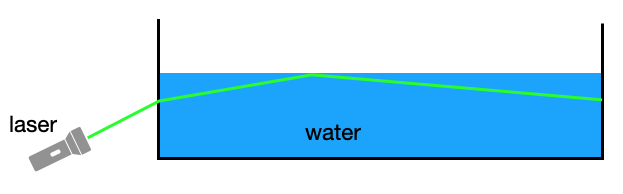
\includegraphics[width=0.59\linewidth,height=\textheight,keepaspectratio]{geometrical-optics/../assets/images/reflection/basin_tir.png}
\begin{center}
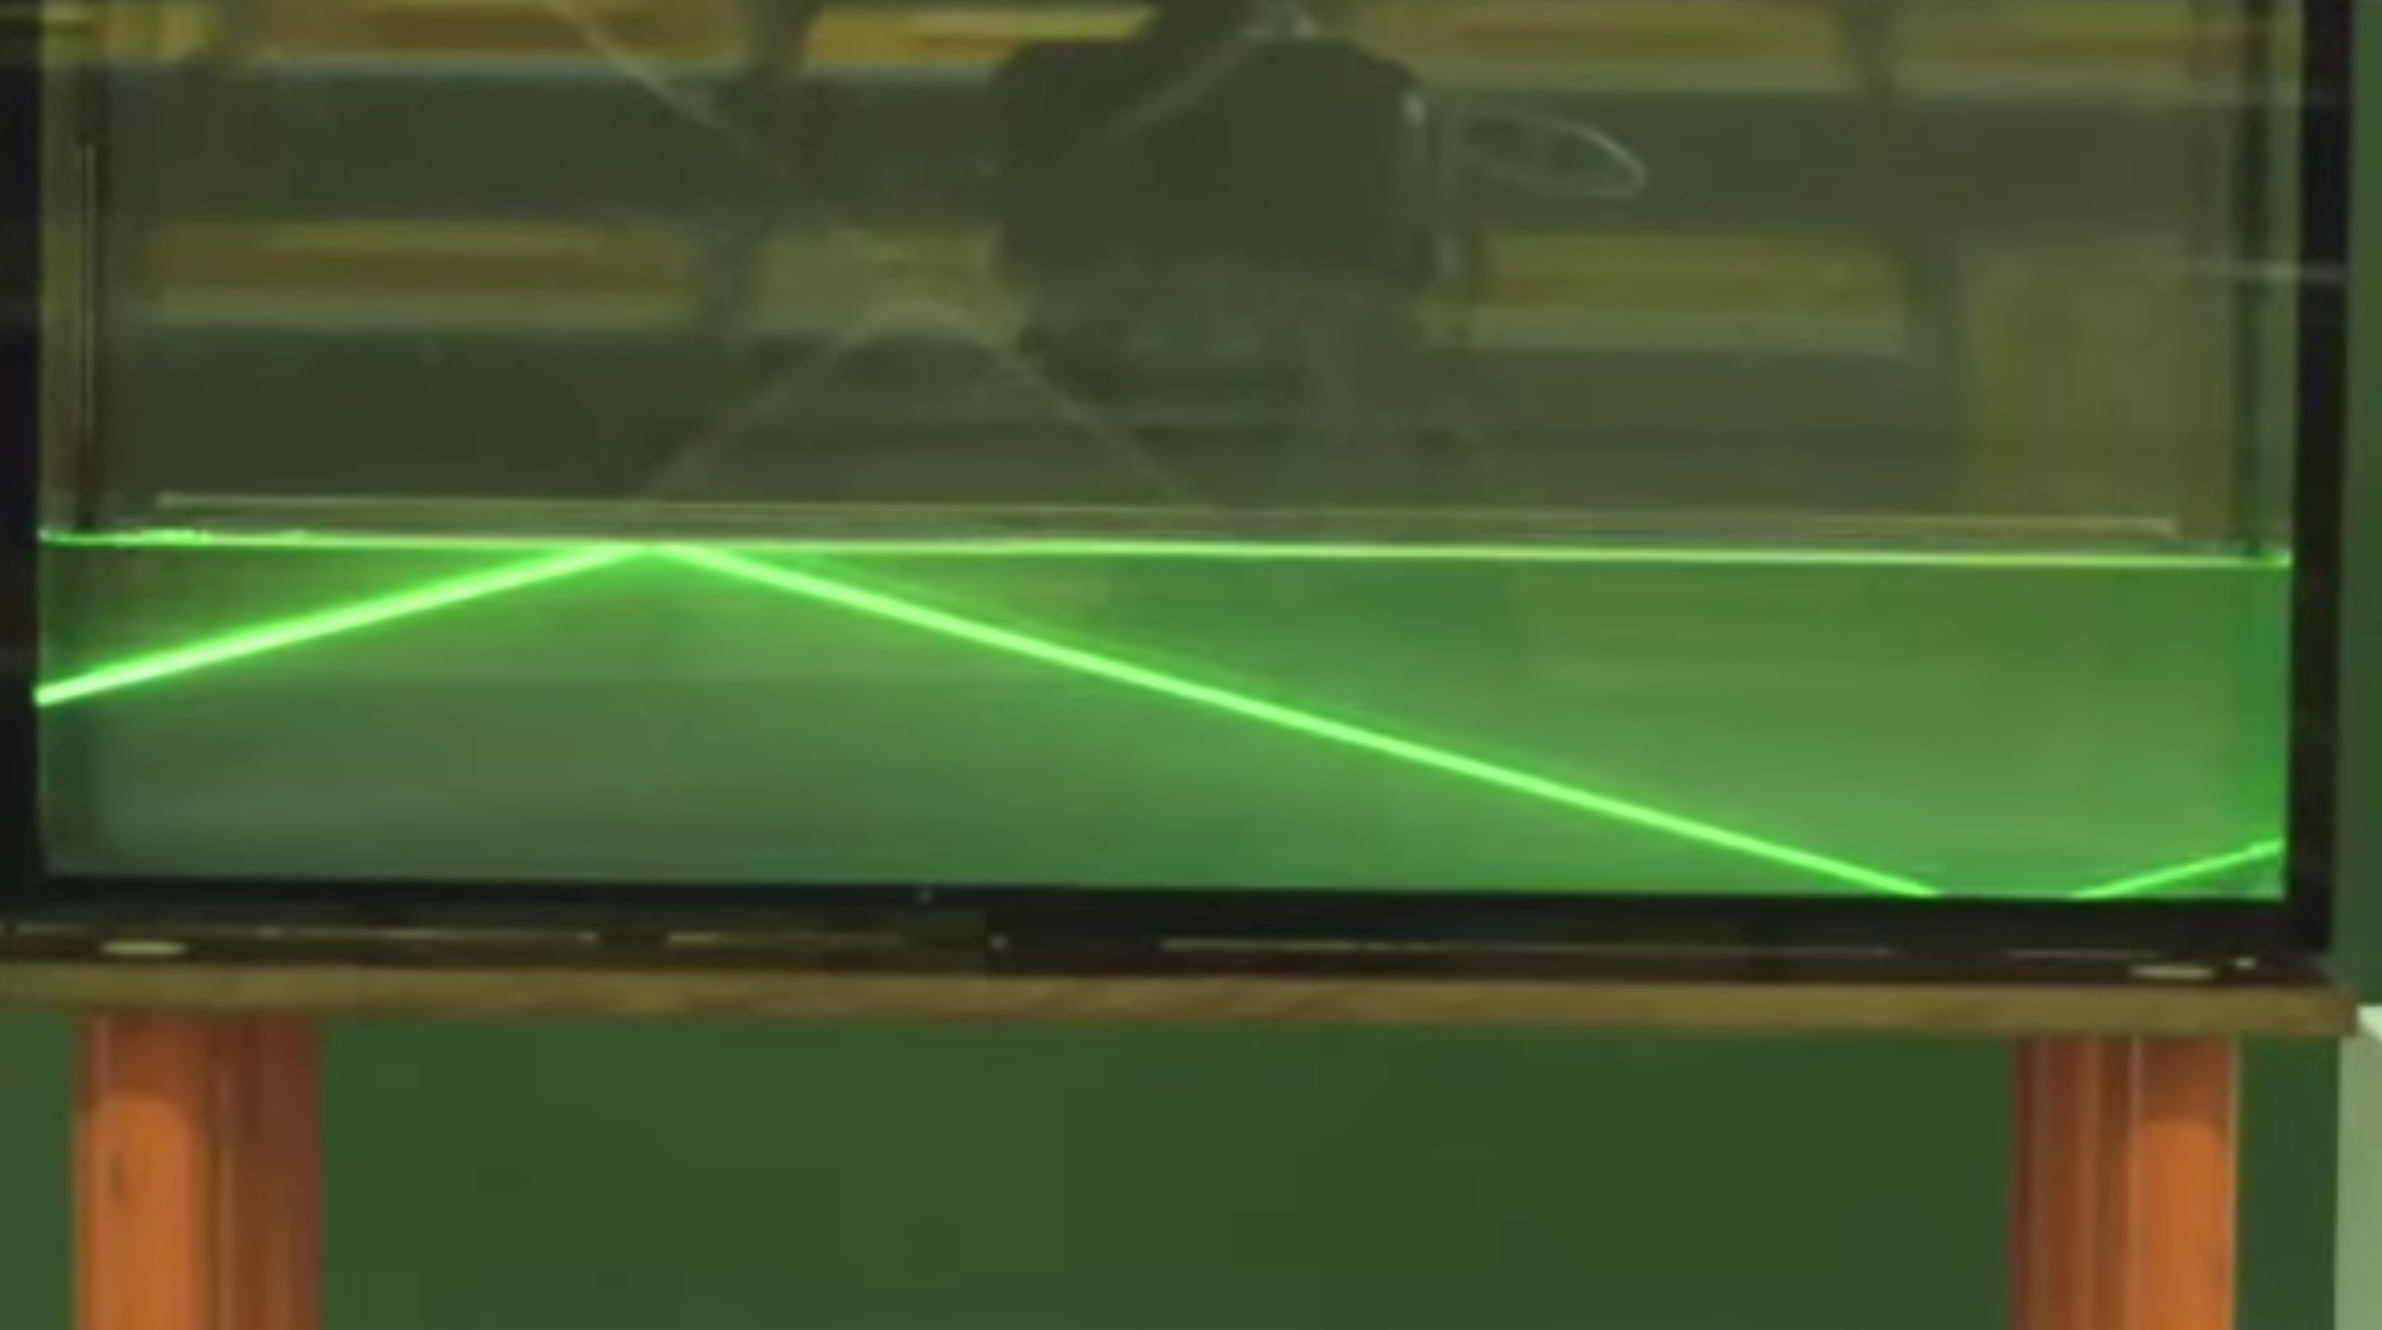
\includegraphics[width=0.4\linewidth,height=\textheight,keepaspectratio]{geometrical-optics/../assets/images/reflection/tir_basin.png}
\end{center}

But you could try that yourself also in the bath tub diving below the
water surface.

Total internal reflection has numerous practical applications:

\begin{enumerate}
\def\labelenumi{\arabic{enumi}.}
\tightlist
\item
  Fiber optic communications: Light signals can travel long distances
  with minimal loss through optical fibers.
\item
  Optical instruments: Prisms in binoculars and telescopes use total
  internal reflection to manipulate light paths.
\item
  Gemstones: The sparkle of diamonds is enhanced by total internal
  reflection trapping light within the stone.
\item
  Medical endoscopes: Total internal reflection helps guide light
  through flexible tubes for internal imaging.
\end{enumerate}

\textbf{Optical Fibers and Total Internal Reflection}

Total internal reflection plays a crucial role in modern
telecommunications, particularly in optical fibers, which are also part
of many experimental setups. These fibers are essentially ultra-thin
glass wires, ranging in diameter from a few micrometers to several
hundred micrometers, designed to transport light over long distances
with minimal loss.

The structure of an optical fiber is key to its function:

\begin{enumerate}
\def\labelenumi{\arabic{enumi}.}
\tightlist
\item
  Core: A central glass core with a refractive index \(n_1\)
\item
  Cladding: A surrounding layer with a slightly lower refractive index
  \(n_2\)
\end{enumerate}

This difference in refractive indices is what allows total internal
reflection to occur within the fiber.

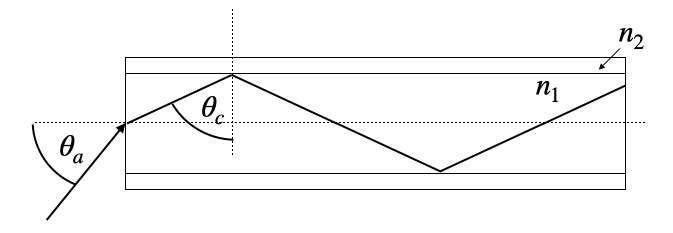
\includegraphics[width=0.59\linewidth,height=\textheight,keepaspectratio]{geometrical-optics/../assets/images/reflection/fiber.png}
\begin{center}
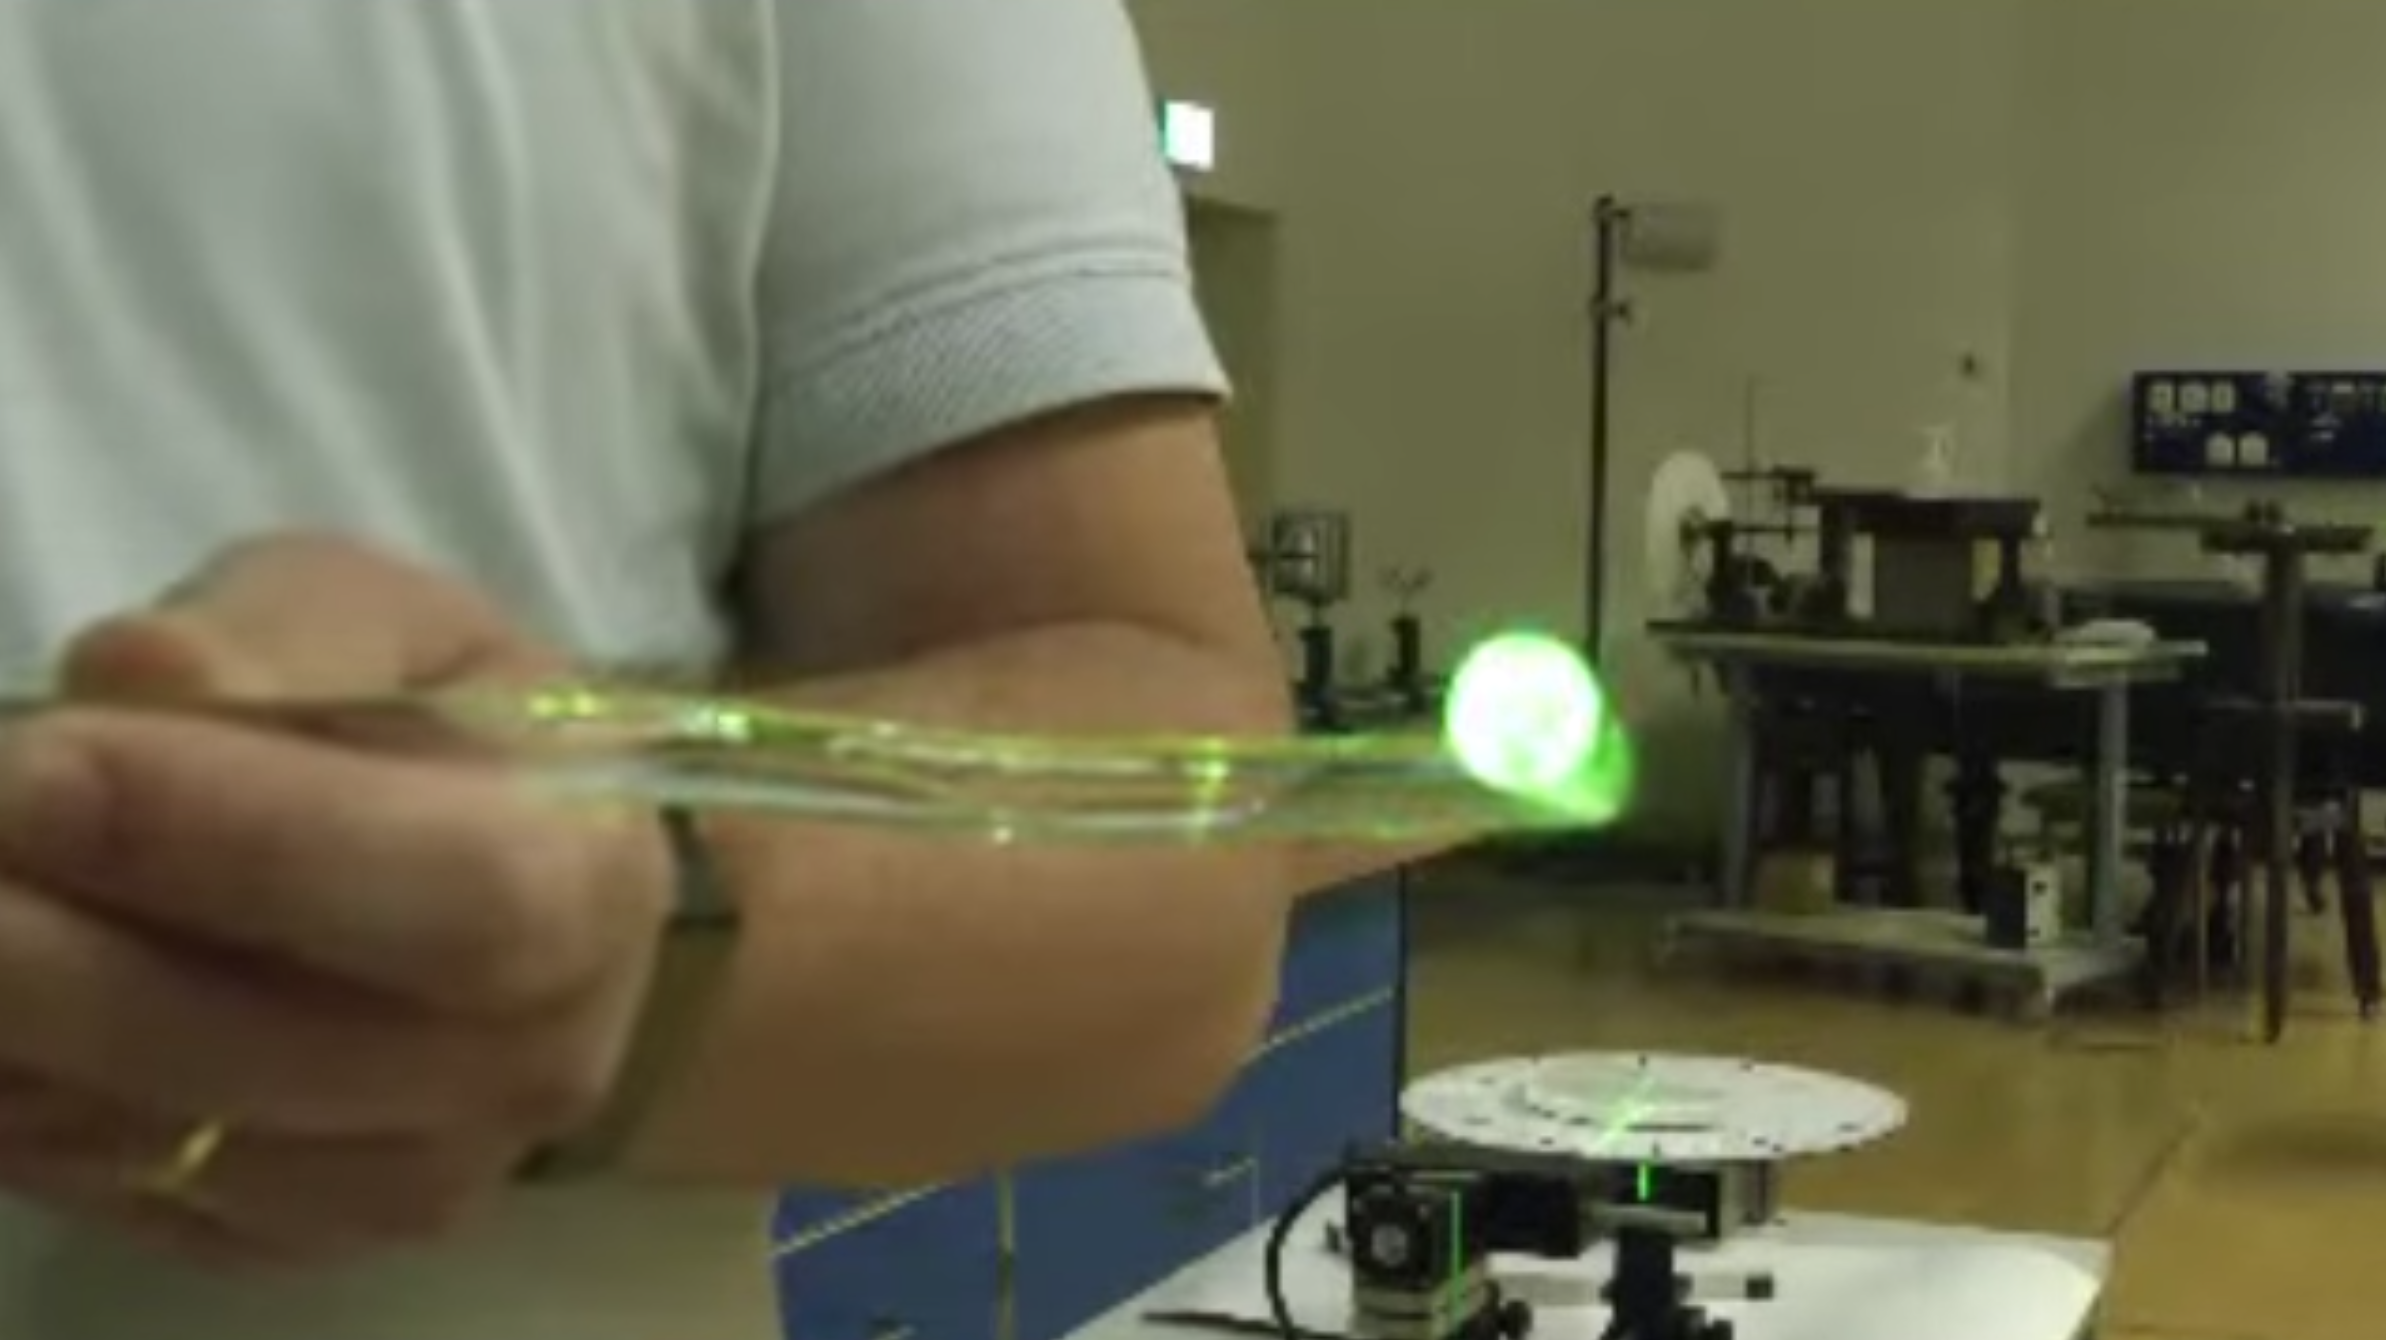
\includegraphics[width=0.4\linewidth,height=\textheight,keepaspectratio]{geometrical-optics/../assets/images/reflection/tir_rod.png}
\end{center}

For light to propagate effectively through the fiber, it must enter at
an angle that ensures total internal reflection at the core-cladding
interface. This leads to the concept of the acceptance angle,
\(\theta_a\), which is the maximum angle at which light can enter the
fiber and still undergo total internal reflection.

To characterize this acceptance angle, optical engineers use a parameter
called the \textbf{Numerical Aperture (NA)}.

\begin{tcolorbox}[enhanced jigsaw, breakable, toptitle=1mm, bottomrule=.15mm, colbacktitle=quarto-callout-tip-color!10!white, title=\textcolor{quarto-callout-tip-color}{\faLightbulb}\hspace{0.5em}{Numerical Aperture}, arc=.35mm, rightrule=.15mm, bottomtitle=1mm, opacityback=0, toprule=.15mm, coltitle=black, leftrule=.75mm, opacitybacktitle=0.6, colback=white, left=2mm, titlerule=0mm, colframe=quarto-callout-tip-color-frame]

The Numerical Aperture of a fiber is defined as the sine of the maximum
acceptance angle:

\begin{equation}
NA = \sin(\theta_a) = \sqrt{n_1^2 - n_2^2}
\end{equation}

\end{tcolorbox}

This equation relates the NA directly to the refractive indices of the
core and cladding. The derivation of this formula involves applying
Snell's law at the air-fiber interface and at the core-cladding
interface, then using the condition for total internal reflection.

In practice, typical values for the refractive indices might be
\(n_1 = 1.475\) for the core and \(n_2 = 1.46\) for the cladding.
Plugging these into our equation:

\begin{equation}
NA = \sqrt{1.475^2 - 1.46^2} \approx 0.2
\end{equation}

This means that light entering the fiber within a cone of about 11.5°
(arcsin(0.2)) from the fiber's axis will be transmitted through the
fiber via total internal reflection.

The NA is an important parameter in fiber optic design:

\begin{enumerate}
\def\labelenumi{\arabic{enumi}.}
\tightlist
\item
  It determines the light-gathering ability of the fiber.
\item
  It affects the fiber's bandwidth and its susceptibility to certain
  types of signal distortion.
\item
  It influences how easily the fiber can be coupled to light sources and
  other fibers.
\end{enumerate}

Optical fibers come in various types, each optimized for different
applications. Some fibers are designed to transmit light over long
distances with minimal loss, while others are engineered for specific
wavelengths or to guide light in unusual ways. The figure below shows a
few examples of optical fiber types.

\begin{figure}

\centering{

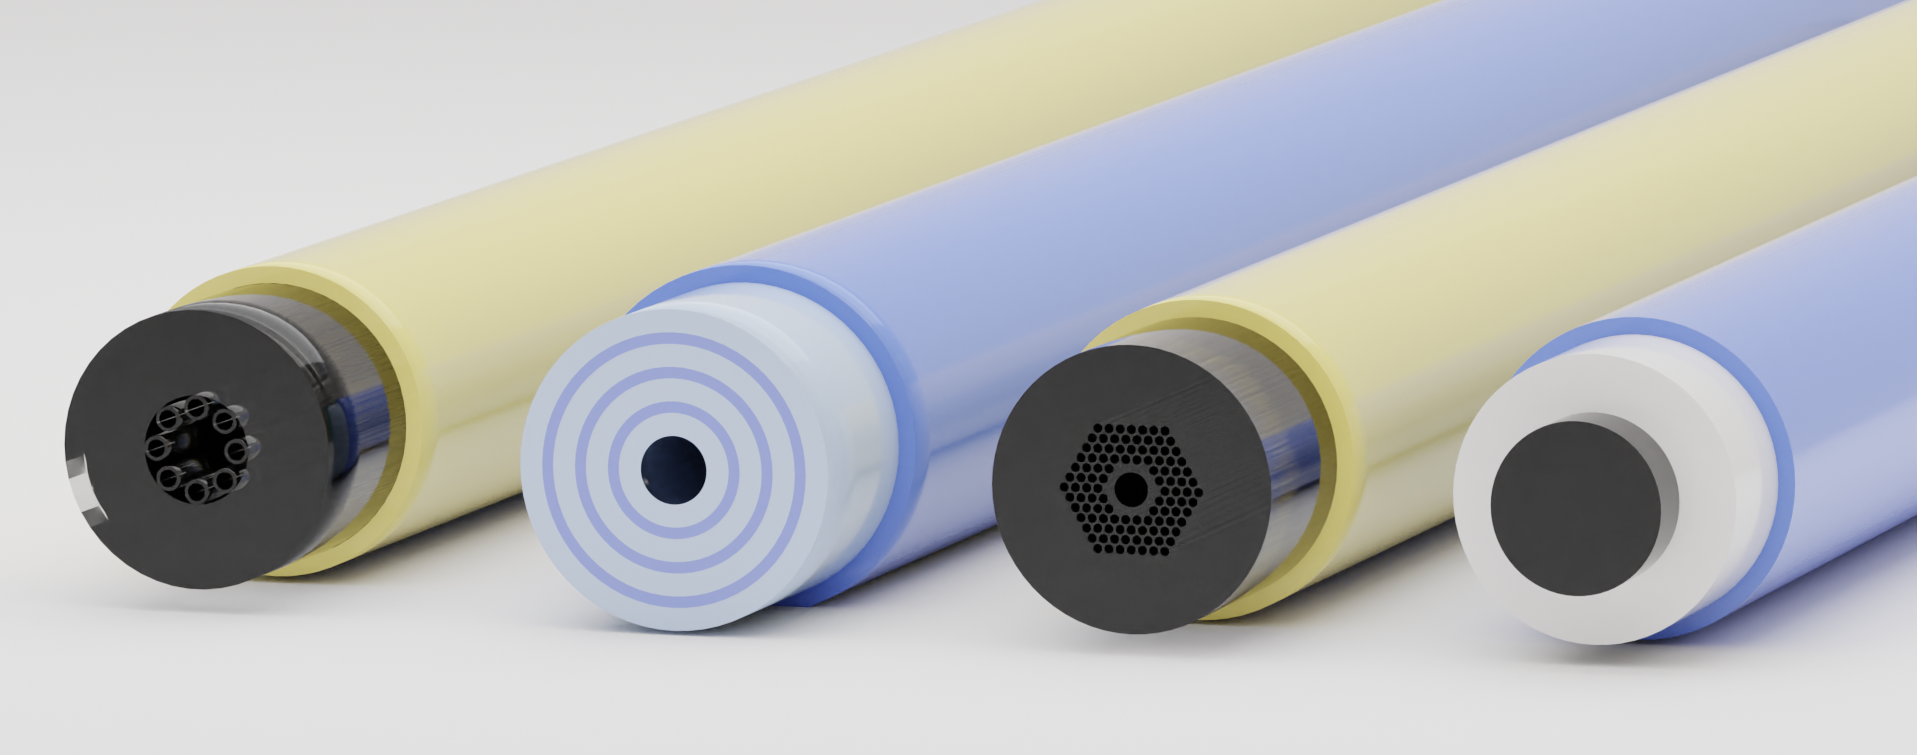
\includegraphics[width=1\linewidth,height=\textheight,keepaspectratio]{geometrical-optics/../assets/images/reflection/fibers.png}

}

\caption{\label{fig-fiber-types}Rendering of different optical fibers
types (from left to right): Hollow core optical fiber, hollow core bragg
fiber, photonic crystal fiber, conventional fiber}

\end{figure}%

\subsection{Fermat's Principle for Inhomogeneous
Media}\label{fermats-principle-for-inhomogeneous-media}

While before we have considered Fermat's principle for the special case
of refraction and light propagation in a homogeneous medium, we can
define a more general version of it correponding to the following
situation also involving an inhomogeneous refractive index
\(n(\vec{r})\).

\begin{figure}

\centering{

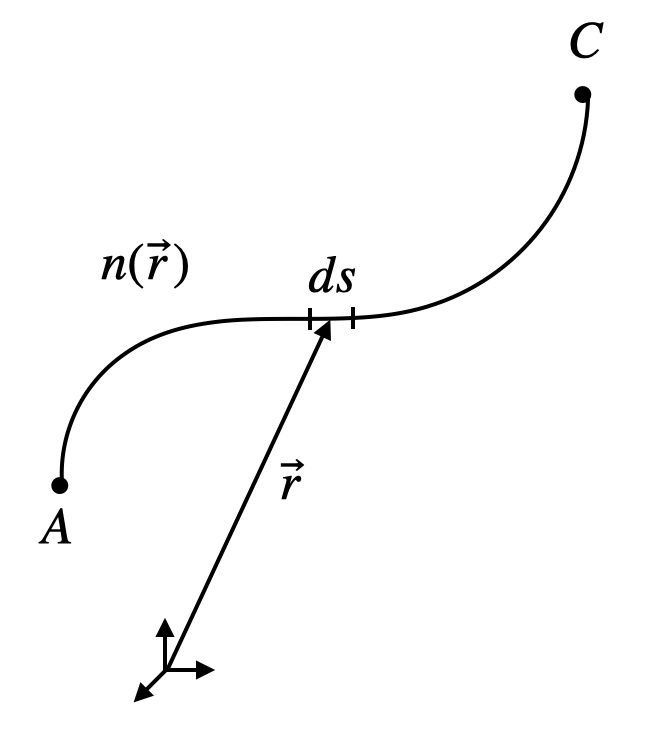
\includegraphics[width=0.4\linewidth,height=\textheight,keepaspectratio]{geometrical-optics/../assets/images/reflection/fermat_general.png}

}

\caption{\label{fig-fermat-general}Sketch for a general description of
Fermat's principle}

\end{figure}%

For this general scenario of light traveling along a path, we can define
an optical path length (OPL) as

\begin{equation}
\text{OPL} = \int\limits_{A}^{C} n(\mathbf{r}) \mathrm ds=0,
\end{equation}

with a varying refractive index \(n(\mathbf{r})\). Fermat's Principle
states that the actual path taken by the light makes the OPL stationary:

\[
\delta \left( \int_A^B n(\mathbf{r}) \, ds \right) = 0
\]

Using the calculus of variations, this leads to the Euler-Lagrange
equation for the path of light. In Cartesian coordinates, if the path is
parameterized by \(\mathbf{r}(s) = (x(s), y(s), z(s))\), the
Euler-Lagrange equations become:

\[
\frac{d}{ds} \left( n \frac{d\mathbf{r}}{ds} \right) = \nabla n
\]

where \(\nabla n\) is the gradient of the refractive index. This
equation describes how the light ray bends in response to changes in the
refractive index of the medium.

Fermat's Principle is a cornerstone of geometrical optics and has
applications in designing optical systems, understanding mirages, and
analyzing the behavior of light in various media.

\begin{tcolorbox}[enhanced jigsaw, breakable, toptitle=1mm, bottomrule=.15mm, colbacktitle=quarto-callout-note-color!10!white, title=\textcolor{quarto-callout-note-color}{\faInfo}\hspace{0.5em}{F=ma Optics: Mathematical Analogy with Newton's Second Law}, arc=.35mm, rightrule=.15mm, bottomtitle=1mm, opacityback=0, toprule=.15mm, coltitle=black, leftrule=.75mm, opacitybacktitle=0.6, colback=white, left=2mm, titlerule=0mm, colframe=quarto-callout-note-color-frame]

The differential form of Fermat's principle bears a striking
mathematical resemblance to Newton's second law of motion, F = ma. This
analogy provides a beautiful connection between mechanics and optics,
sometimes referred to as ``F=ma optics.''

Recall that the differential form of Fermat's principle is:

\[
\frac{d}{ds}\left(n\frac{d\mathbf{r}}{ds}\right) = \nabla n
\]

Now consider Newton's second law in its most general form:

\[
\frac{d}{dt}\left(m\mathbf{v}\right) = \mathbf{F}
\]

where \(\mathbf{v} = \frac{d\mathbf{r}}{dt}\) is the velocity.

\textbf{The Mathematical Analogy:}

The parallel between these equations becomes clear when we make the
following correspondences:

\begin{longtable}[]{@{}
  >{\raggedright\arraybackslash}p{(\linewidth - 2\tabcolsep) * \real{0.5789}}
  >{\raggedright\arraybackslash}p{(\linewidth - 2\tabcolsep) * \real{0.4211}}@{}}
\toprule\noalign{}
\begin{minipage}[b]{\linewidth}\raggedright
Mechanics
\end{minipage} & \begin{minipage}[b]{\linewidth}\raggedright
Optics
\end{minipage} \\
\midrule\noalign{}
\endhead
\bottomrule\noalign{}
\endlastfoot
Time \(t\) & Arc length \(s\) \\
Mass \(m\) & Refractive index \(n\) \\
Velocity \(\mathbf{v} = \frac{d\mathbf{r}}{dt}\) & Ray direction
\(\frac{d\mathbf{r}}{ds}\) \\
Momentum \(m\mathbf{v}\) & Optical momentum
\(n\frac{d\mathbf{r}}{ds}\) \\
Force \(\mathbf{F}\) & Gradient of refractive index \(\nabla n\) \\
\end{longtable}

In this analogy:

\begin{enumerate}
\def\labelenumi{\arabic{enumi}.}
\item
  \textbf{The role of mass in mechanics is played by the refractive
  index in optics.} Just as a massive particle has more inertia and
  resists changes in motion, a light ray in a high-refractive-index
  medium is more ``resistant'' to bending.
\item
  \textbf{The role of force is played by the gradient of the refractive
  index.} Just as a force causes a particle to accelerate (change its
  momentum), a gradient in refractive index causes a light ray to bend
  (change its optical momentum).
\item
  \textbf{Arc length in optics plays the role of time in mechanics.} The
  evolution of the light ray's path with respect to arc length follows
  the same mathematical structure as the evolution of a particle's
  trajectory with respect to time.
\end{enumerate}

This analogy is more than just a mathematical curiosity---it reveals a
deep connection between different areas of physics. Both Fermat's
principle and Newton's laws can be derived from more fundamental
variational principles (Fermat's principle of least time and Hamilton's
principle of least action, respectively), which is why they share the
same mathematical structure.

\textbf{Practical Implications:}

This analogy allows us to:

\begin{itemize}
\tightlist
\item
  Use intuition from mechanics to understand optical phenomena
\item
  Apply mathematical techniques from classical mechanics to solve optics
  problems
\item
  Design optical systems by thinking about ``forces'' acting on light
  rays
\end{itemize}

For example, a graded-index fiber can be thought of as creating an
``optical force'' that pulls light rays back toward the fiber axis, much
like a spring force in a harmonic oscillator pulls a mass back to
equilibrium.

\end{tcolorbox}

\subsection{Example: Photothermal
Microscopy}\label{example-photothermal-microscopy}

Photothermal microscopy is a powerful optical technique that exploits
the refractive index changes induced by localized heating. When a
material absorbs light, it converts the optical energy into heat,
creating a temperature gradient in the surrounding medium. This
temperature gradient produces a corresponding gradient in the refractive
index, which can deflect probe light beams passing through the
region---a phenomenon that can be understood and predicted using
Fermat's principle in inhomogeneous media.

The technique works by using two laser beams: a heating (pump) beam that
is absorbed by the sample, creating a thermal gradient, and a probe beam
that is deflected by the resulting refractive index gradient. By
detecting this deflection, one can obtain information about the
absorption properties of the sample with extremely high sensitivity,
even detecting single nanoparticles or molecules.

The images below demonstrate this principle beautifully. A copper sphere
embedded in acrylic glass is heated by a laser, creating a radial
temperature gradient around it. This gradient produces a corresponding
refractive index gradient that deflects a probe laser beam. The
distortion becomes clearly visible when viewing a regular grid pattern
through the acrylic block---when the heating is switched on, the grid
pattern warps due to the refractive index changes, and returns to normal
when the heating is switched off.

\begin{figure}

\begin{minipage}{0.50\linewidth}

\pandocbounded{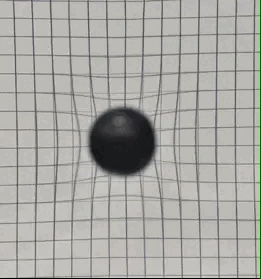
\includegraphics[keepaspectratio]{geometrical-optics/img/cube_PT.png}}

\subcaption{\label{}Photothermal deflection around a heated copper
sphere in acrylic glass.}
\end{minipage}%
%
\begin{minipage}{0.50\linewidth}
\end{minipage}%
\newline
\begin{minipage}{0.50\linewidth}

\pandocbounded{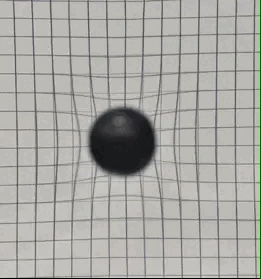
\includegraphics[keepaspectratio]{geometrical-optics/img/cube_PT.png}}

\subcaption{\label{}Grid distortion when viewing through the heated
acrylic block.}
\end{minipage}%

\caption{\label{fig-photothermal}Photothermal deflection demonstration.
(Left) A copper sphere embedded in acrylic glass creates a refractive
index gradient when heated by a laser. (Right) The resulting distortion
becomes visible when viewing a regular grid pattern through the heated
block.}

\end{figure}%

This demonstration illustrates how Fermat's principle applies to
inhomogeneous media: the light rays bend continuously as they traverse
regions with varying refractive index, following paths that make the
optical path length stationary. The heating-induced refractive index
gradient \(\nabla n\) acts as an ``optical force'' that deflects the
light rays, just as described by the differential form of Fermat's
principle:
\(\frac{d}{ds}\left(n\frac{d\mathbf{r}}{ds}\right) = \nabla n\).

\begin{tcolorbox}[enhanced jigsaw, breakable, toptitle=1mm, bottomrule=.15mm, colbacktitle=quarto-callout-tip-color!10!white, title=\textcolor{quarto-callout-tip-color}{\faLightbulb}\hspace{0.5em}{Fermat's Principle and Snells Law}, arc=.35mm, rightrule=.15mm, bottomtitle=1mm, opacityback=0, toprule=.15mm, coltitle=black, leftrule=.75mm, opacitybacktitle=0.6, colback=white, left=2mm, titlerule=0mm, colframe=quarto-callout-tip-color-frame]

We would like to apply Fermat's principle to derive Snell's law, which
is a more lengthy calculation. To do this, we consider a light ray
traveling from point \(A\) in medium 1 (with refractive index \(n_1\))
to point \(C\) in medium 2 (with refractive index \(n_2\)), crossing the
interface at point \(B\). Let the coordinates of points \(A\), \(B\),
and \(C\) be \((x_A, y_A)\), \((x_B, y_B)\), and \((x_C, y_C)\),
respectively. Assume the interface between the two media is at
\(y = y_B\). The optical path length (OPL) is given by:

\[
\delta \int_{A}^{C} n(\vec{r}) \, ds = 0,
\]

where \(n(\vec{r})\) is the refractive index at position \(\vec{r}\),
and \(ds\) is an infinitesimal element of the path.

Consider a light ray traveling from point \(A\) in medium 1 (with
refractive index \(n_1\)) to point \(C\) in medium 2 (with refractive
index \(n_2\)), crossing the interface at point \(B\). Let the
coordinates of points \(A\), \(B\), and \(C\) be \((x_A, y_A)\),
\((x_B, y_B)\), and \((x_C, y_C)\), respectively. Assume the interface
between the two media is at \(y = y_B\).

\subsubsection{Optical Path Length}\label{optical-path-length}

The optical path length (OPL) is given by:

\[
\text{OPL} = n_1 \int_{A}^{B} ds_1 + n_2 \int_{B}^{C} ds_2,
\]

where \(ds_1\) and \(ds_2\) are the infinitesimal path lengths in media
1 and 2, respectively.

\subsubsection{Path Lengths}\label{path-lengths}

The path lengths \(ds_1\) and \(ds_2\) can be expressed in terms of the
coordinates:

\[
ds_1 = \sqrt{(dx_1)^2 + (dy_1)^2}, \quad ds_2 = \sqrt{(dx_2)^2 + (dy_2)^2}.
\]

Since the interface is at \(y = y_B\), we have \(dy_1 = y_B - y_A\) and
\(dy_2 = y_C - y_B\). The total optical path length is:

\[
\text{OPL} = n_1 \sqrt{(x_B - x_A)^2 + (y_B - y_A)^2} + n_2 \sqrt{(x_C - x_B)^2 + (y_C - y_B)^2}.
\]

\subsubsection{Applying Fermat's
Principle}\label{applying-fermats-principle}

To find the stationary path, we take the variation of the OPL with
respect to \(x_B\):

\[
\delta \text{OPL} = \delta \left[ n_1 \sqrt{(x_B - x_A)^2 + (y_B - y_A)^2} + n_2 \sqrt{(x_C - x_B)^2 + (y_C - y_B)^2} \right] = 0.
\]

Taking the derivative with respect to \(x_B\):

\[
\frac{\partial}{\partial x_B} \left[ n_1 \sqrt{(x_B - x_A)^2 + (y_B - y_A)^2} + n_2 \sqrt{(x_C - x_B)^2 + (y_C - y_B)^2} \right] = 0.
\]

\subsubsection{Differentiating}\label{differentiating}

Differentiating each term separately:

\[
n_1 \frac{\partial}{\partial x_B} \sqrt{(x_B - x_A)^2 + (y_B - y_A)^2} + n_2 \frac{\partial}{\partial x_B} \sqrt{(x_C - x_B)^2 + (y_C - y_B)^2} = 0.
\]

Using the chain rule:

\[
n_1 \frac{x_B - x_A}{\sqrt{(x_B - x_A)^2 + (y_B - y_A)^2}} + n_2 \frac{x_B - x_C}{\sqrt{(x_C - x_B)^2 + (y_C - y_B)^2}} = 0.
\]

\subsubsection{Simplifying}\label{simplifying}

Let \(\theta_1\) be the angle of incidence and \(\theta_2\) be the angle
of refraction. Then:

\[
\sin \theta_1 = \frac{x_B - x_A}{\sqrt{(x_B - x_A)^2 + (y_B - y_A)^2}}, \quad \sin \theta_2 = \frac{x_C - x_B}{\sqrt{(x_C - x_B)^2 + (y_C - y_B)^2}}.
\]

Substituting these into the equation:

\[
n_1 \sin \theta_1 + n_2 \sin \theta_2 = 0.
\]

Since \(\sin \theta_2\) is in the opposite direction, we have:

\[
n_1 \sin \theta_1 = n_2 \sin \theta_2.
\]

This is Snell's law, which describes the relationship between the angles
of incidence and refraction when light passes from one medium to
another.

\subsubsection{Conclusion}\label{conclusion}

By applying Fermat's principle and taking the variation of the optical
path length, we have derived Snell's law:

\[
n_1 \sin \theta_1 = n_2 \sin \theta_2.
\]

This demonstrates how the principle of least time leads to the
well-known law of refraction in optics.

\end{tcolorbox}

\begin{tcolorbox}[enhanced jigsaw, breakable, toptitle=1mm, bottomrule=.15mm, colbacktitle=quarto-callout-tip-color!10!white, title=\textcolor{quarto-callout-tip-color}{\faLightbulb}\hspace{0.5em}{Example: Light in a Graded-Index Medium}, arc=.35mm, rightrule=.15mm, bottomtitle=1mm, opacityback=0, toprule=.15mm, coltitle=black, leftrule=.75mm, opacitybacktitle=0.6, colback=white, left=2mm, titlerule=0mm, colframe=quarto-callout-tip-color-frame]

Consider a medium where the refractive index varies with height \(y\) as
\(n(y) = n_0 \left(1 - \frac{\alpha^2}{2} y^2\right)\). The path of
light in such a medium can be found by using Fermat's principle in
differential form:

\[
\frac{d}{ds}\left (n(\textbf{r})\frac{d\textbf{r}}{ds}\right)=\nabla n(\textbf{r})
\]

Typically, this requires expressing the coordinates in terms of a
parameter, such as \(x(s)\) and \(y(s)\), and then solving the
differential equation. The solution will give the path of light in the
medium. This is difficult and commonly done numerically. In paraxial
optics, when the light is propagating roughly in the direction of \(z\),
the differential element \(ds\) can be approximated as \(dz\) since then

\[
ds=dz\sqrt{1+\left (\frac{dy}{dz}\right )^2+\left (\frac{dx}{dz}\right)^2}\approx dz
\]

which yields

\[
\frac{d}{dz}\left (n\frac{dx}{dz}\right)\approx \frac{\partial n}{\partial x}
\]

and

\[
\frac{d}{dz}\left (n\frac{dy}{dz}\right )\approx \frac{\partial n}{\partial y}
\]

This readily yields the path of light in a homogeneous medium, where
\(n\) is constant. In this case we have

\[
\frac{d^2 x}{dz^2}=\frac{d^2 y}{dz^2}=0
\]

which is true for a straight line. In a graded-index medium with
\(n(y) = n_0 \left(1 - \frac{\alpha^2}{2} y^2\right)\), we have
\(\frac{\partial n}{\partial y} = -n_0 \alpha^2 y\). Under the paraxial
approximation where \(n \approx n_0\) is approximately constant along
the ray, the path of light can be found by solving the differential
equation

\[
n_0 \frac{d^2 y}{dz^2} \approx -n_0 \alpha^2 y
\]

which simplifies to

\[
\frac{d^2 y}{dz^2} \approx -\alpha^2 y
\]

This is reminiscent of the equation of motion of a harmonic oscillator.
The solution is therefore an oscillating function

\[
y(z)=y_0\cos(\alpha z)+\frac{\theta_0}{\alpha}\sin(\alpha z)
\]

where \(y_0\) is the initial position and \(\theta_0\) is the initial
angle of the light ray with respect to the \(z\) axis. This solution
describes the sinusoidal path of light in a graded-index medium with a
parabolic refractive index profile.

\end{tcolorbox}

\begin{tcolorbox}[enhanced jigsaw, breakable, toptitle=1mm, bottomrule=.15mm, colbacktitle=quarto-callout-tip-color!10!white, title=\textcolor{quarto-callout-tip-color}{\faLightbulb}\hspace{0.5em}{Fermat's Principle in Integral and Differential Form}, arc=.35mm, rightrule=.15mm, bottomtitle=1mm, opacityback=0, toprule=.15mm, coltitle=black, leftrule=.75mm, opacitybacktitle=0.6, colback=white, left=2mm, titlerule=0mm, colframe=quarto-callout-tip-color-frame]

We have described Fermat't principle in an integral form specifiying the
optical path length \(S\) as

\[
OPL=\int n(\textbf{r})ds
\]

The path length \(ds\) can be given in terms of two coordinates \(x_1\)
and \(x_2\) parametrized by \(\lambda\) such that

\[
ds=\sqrt{\dot{x}_1^{2}+\dot{x}_2^{2}}d\lambda
\]

where \(\dot{x}_1=\frac{dx_{1}}{d\lambda}\). We can therefore write
Fermat's principle as

\[
\delta OPL=\int\left[\left(\frac{\partial n}{\partial x_i} \delta x_i\right) \sqrt{\dot{x}_1^2+\dot{x}_2^2}+n \frac{1}{\sqrt{\dot{x}_1^2+\dot{x}_2^2}} \dot{x}_i \delta \dot{x}_i\right] d \lambda = 0
\]

To evaluate this integral we would like to integrate by parts. We can
write the integrand as \[
u = n \frac{1}{\sqrt{\dot{x}_1^2+\dot{x}_2^2}} \dot{x}_i
\]

and

\[
dv = \delta \dot{x}_i d\lambda
\]

We can now calculate \(du\) and \(v\) and obtain

\[
du = \frac{d}{d\lambda}\left[n \frac{1}{\sqrt{\dot{x}_1^2+\dot{x}_2^2}} \dot{x}_i\right] d\lambda
\]

and

\[
v = \delta x_i
\]

With these expressions we can now apply the integration by parts formula
\(\int u dv = uv - \int v du\), we get:

\[
\int n \frac{1}{\sqrt{\dot{x}_1^2+\dot{x}_2^2}} \dot{x}_i \delta \dot{x}_i d\lambda = \left[n \frac{1}{\sqrt{\dot{x}_1^2+\dot{x}_2^2}} \dot{x}_i \delta x_i\right]|_{\lambda_1}^{\lambda_2} - \int \delta x_i \frac{d}{d\lambda}\left[n \frac{1}{\sqrt{\dot{x}_1^2+\dot{x}_2^2}} \dot{x}_i\right] d\lambda
\]

This can be substituted back into the original equation to obtain

\[
\begin{aligned}
\delta OPL &= \int \left[\left(\frac{\partial n}{\partial x_i} \delta x_i\right) \sqrt{\dot{x}_1^2+\dot{x}_2^2}\right] d\lambda \\
&+ \left[n \frac{1}{\sqrt{\dot{x}_1^2+\dot{x}_2^2}} \dot{x}_i \delta x_i\right]|_{\lambda_1}^{\lambda_2} \\
&- \int \delta x_i \frac{d}{d\lambda}\left[n \frac{1}{\sqrt{\dot{x}_1^2+\dot{x}_2^2}} \dot{x}_i\right] d\lambda = 0
\end{aligned}
\]

After rearranging the terms we get

\[
\begin{aligned}
\delta OPL &= \int \left\{\frac{\partial n}{\partial x_i} \sqrt{\dot{x}_1^2+\dot{x}_2^2} - \frac{d}{d\lambda}\left[n \frac{1}{\sqrt{\dot{x}_1^2+\dot{x}_2^2}} \dot{x}_i\right]\right\} \delta x_i d\lambda \\
&+ \left[n \frac{1}{\sqrt{\dot{x}_1^2+\dot{x}_2^2}} \dot{x}_i \delta x_i\right]|_{\lambda_1}^{\lambda_2} = 0
\end{aligned}
\]

and therefore finally

\[
\delta OPL=\int\left[\left(\frac{\partial n}{\partial x_i}\right) \sqrt{\dot{x}_1{ }^2+\dot{x}_2{ }^2}-\frac{d}{d \lambda}\left(n \frac{1}{\sqrt{\dot{x}_1^2+\dot{x}_2^2}} \dot{x}_i\right)\right] \delta x_i d \lambda+\text { boundary terms }
\]

for which we choose the parameter \(\lambda\) such that the boundary
terms vanish.

\[
\lambda=s
\]

such that

\[
\sqrt{\dot{x}_1^2+\dot{x}_2^2}=1
\]

and finally leads to the Euler-Lagrange equation

\[
\left(\frac{\partial n}{\partial x_i}\right)-\frac{d}{d s}\left(n \dot{x}_i\right)=0
\]

which is the differential form of the Fermat's principle.

\end{tcolorbox}

\chapter{Optical Elements Part I}\label{optical-elements-part-i}

\section{Mirrors}\label{mirrors}

\subsection{Plane Mirrors}\label{plane-mirrors}

When light radiates from a point \(P\) and reflects off a mirror, as
shown in the image, the reflected rays diverge but appear to originate
from a point \(P'\) located behind the mirror. According to the law of
reflection, this image point is positioned at the same distance behind
the mirror as the original object point is in front of it. As a result,
an observer receiving these reflected rays, such as on their retina,
perceives the point as if it were situated behind the mirror, even
though no light actually travels behind the mirror surface.

\begin{figure}

\begin{minipage}{0.44\linewidth}

\centering{

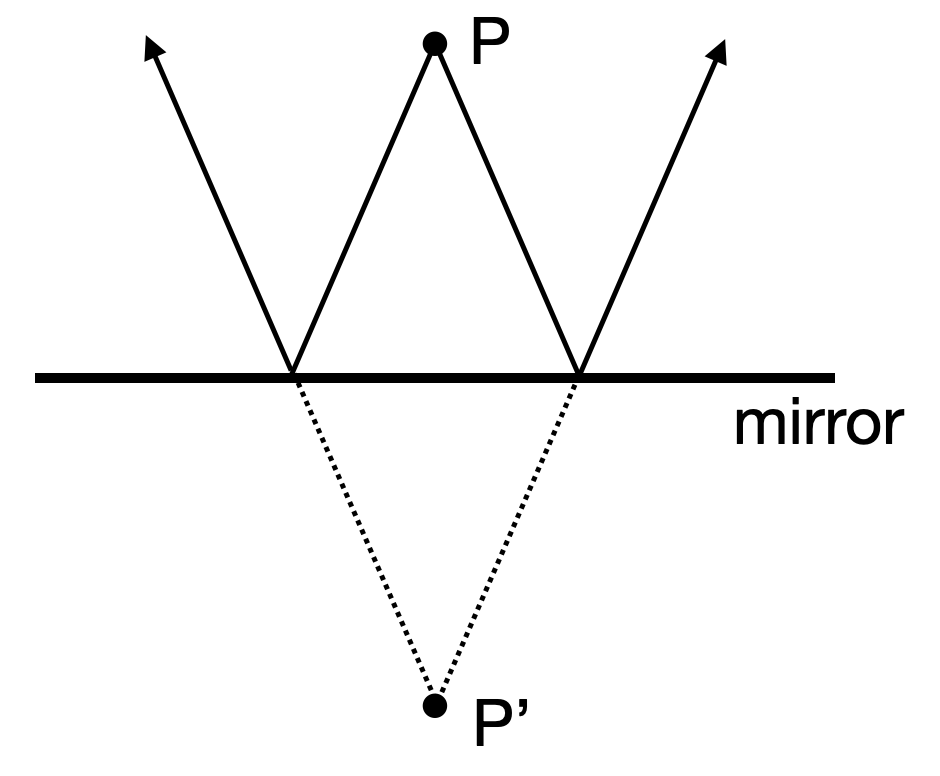
\includegraphics[width=0.8\linewidth,height=\textheight,keepaspectratio]{geometrical-optics/img/plane_mirror.png}

}

\subcaption{\label{fig-plane-mirror}}

\end{minipage}%
%
\begin{minipage}{0.56\linewidth}

\centering{

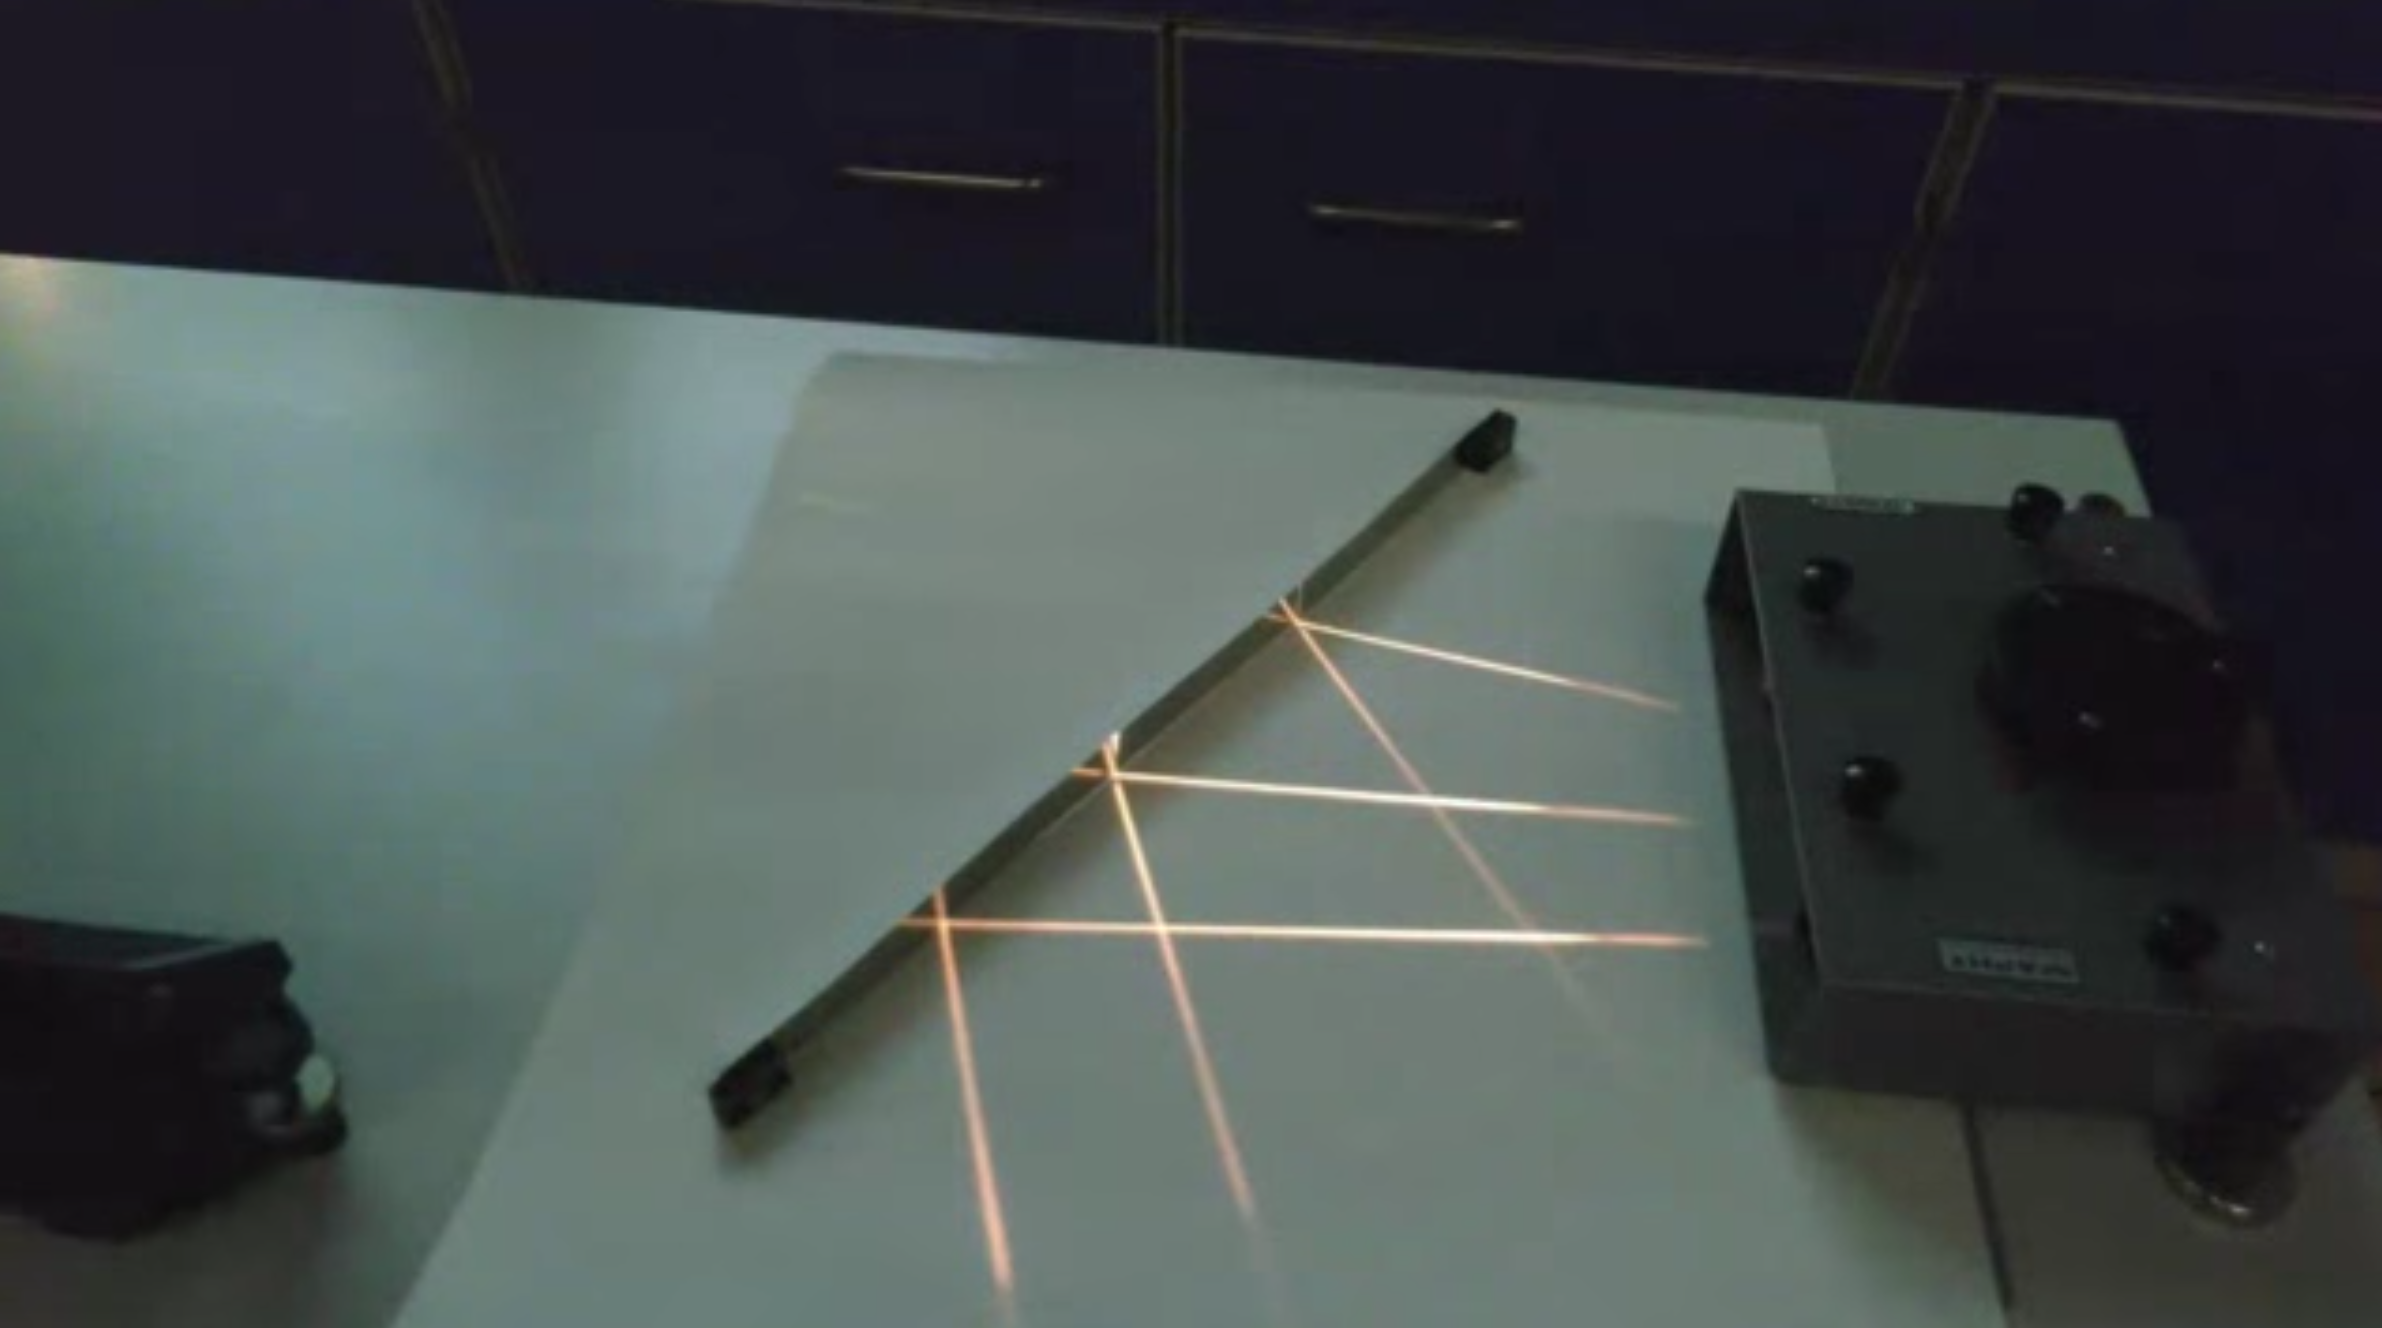
\includegraphics[width=1\linewidth,height=\textheight,keepaspectratio]{geometrical-optics/img/reflection_plane.png}

}

\subcaption{\label{fig-reflection-plane}}

\end{minipage}%

\caption{\label{fig-plane-mirror-combined}Image formation on a plane
mirror.}

\end{figure}%

When multiple points of an object emit light towards the mirror, this
principle applies to each point. As a result, the entire object appears
as an image behind the mirror. Since each point of the image is
equidistant from the mirror as its corresponding object point, the image
has the same size as the object. This leads to the definition of
magnification as:

\[
M=\frac{h_{\text{image}}}{h_{\text{object}}}
\]

\begin{figure}

\centering{

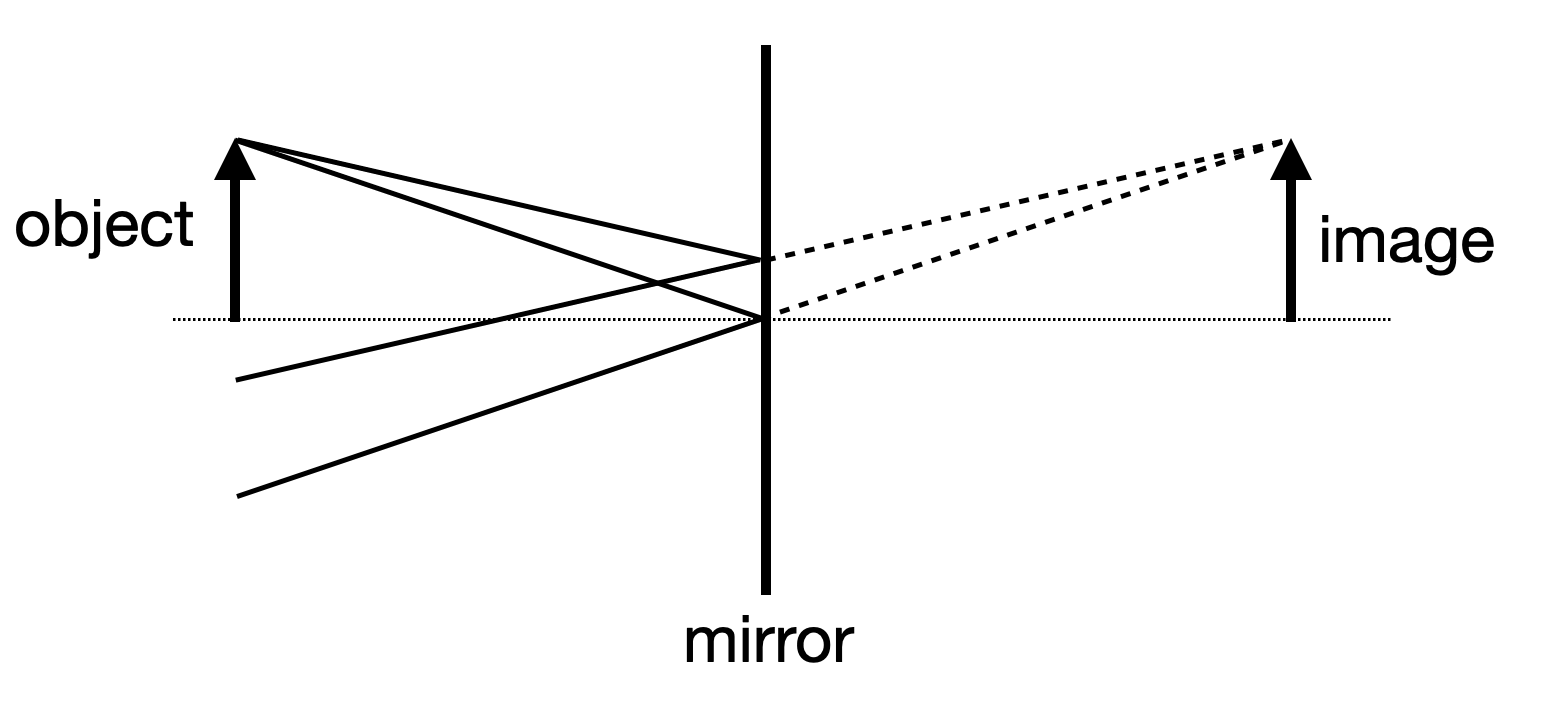
\includegraphics[width=0.6\linewidth,height=\textheight,keepaspectratio]{geometrical-optics/img/image_plane_mirror.png}

}

\caption{\label{fig-plane-mirror}Image formation on a plane mirror.}

\end{figure}%

\begin{tcolorbox}[enhanced jigsaw, breakable, toptitle=1mm, bottomrule=.15mm, colbacktitle=quarto-callout-note-color!10!white, title=\textcolor{quarto-callout-note-color}{\faInfo}\hspace{0.5em}{Virtual Images}, arc=.35mm, rightrule=.15mm, bottomtitle=1mm, opacityback=0, toprule=.15mm, coltitle=black, leftrule=.75mm, opacitybacktitle=0.6, colback=white, left=2mm, titlerule=0mm, colframe=quarto-callout-note-color-frame]

A virtual image is an optical illusion where light rays appear to come
from a point, but don't actually converge there. Unlike real images,
virtual images can't be projected onto a screen. They're commonly seen
in plane mirrors, convex mirrors, and when objects are closer to a lens
than its focal point. \textbf{Remember: for virtual images, light rays
only seem to originate from the image when traced backwards.}

\end{tcolorbox}

\begin{tcolorbox}[enhanced jigsaw, breakable, toptitle=1mm, bottomrule=.15mm, colbacktitle=quarto-callout-note-color!10!white, title=\textcolor{quarto-callout-note-color}{\faInfo}\hspace{0.5em}{Real Images}, arc=.35mm, rightrule=.15mm, bottomtitle=1mm, opacityback=0, toprule=.15mm, coltitle=black, leftrule=.75mm, opacitybacktitle=0.6, colback=white, left=2mm, titlerule=0mm, colframe=quarto-callout-note-color-frame]

A real image forms when light rays actually meet at a point after
reflection or refraction. These images can be projected onto a screen
because light physically passes through the image location. Real images
are often inverted and occur with concave mirrors and lenses when
objects are beyond the focal point. \textbf{Key point: real images
involve actual convergence of light rays.}

\end{tcolorbox}

\subsection{Concave Mirrors}\label{concave-mirrors}

For a concave mirror (where the reflecting surface is on the inside of
the spherical curve), applying the law of reflection yields interesting
results. Light rays parallel to the optical axis, at a distance \(h\)
from it, are reflected towards the axis and intersect it at a specific
point \(F\). Due to the mirror's symmetry, a parallel ray on the
opposite side of the axis will also converge to this same point \(F\).

\begin{figure}

\centering{

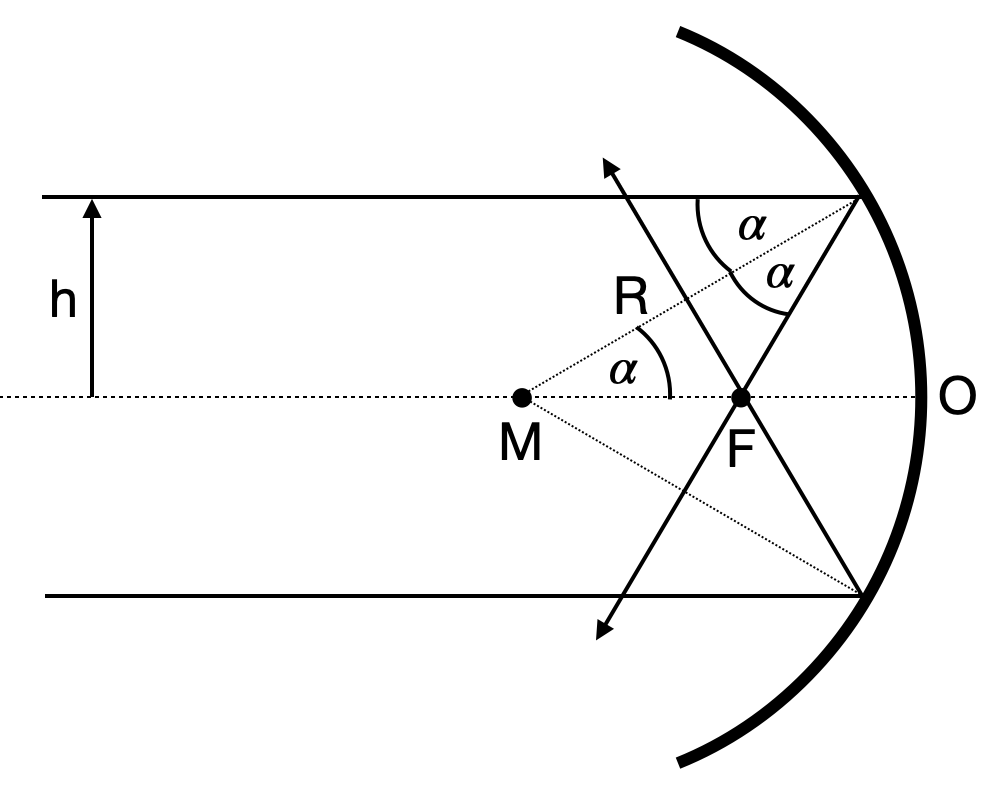
\includegraphics[width=0.6\linewidth,height=\textheight,keepaspectratio]{geometrical-optics/img/concave_mirror.png}

}

\caption{\label{fig-concave-mirror-ray}Reflection of a parallel ray
incident at a height \(h\) from the optical axis on a concave mirror.}

\end{figure}%

We may calculate the position of the point \(F\), e.g.~the distance from
the mirror surface point \(O\), by applying the law of reflection. If
the spherical mirror surface has a radius \(R\), then the distance
between the center of the sphere \(M\) and the point \(F\) is given by

\[FM=\frac{R}{2\cos(\alpha)}\]

Therefore, we can also calculate the distance of the mirror surface from
the point \(F\), which results in

\begin{equation}
OF=R\left (1-\frac{1}{2\cos(\alpha)}\right)=f
\end{equation}

This distance is the so-called focal length of the concave mirror \(f\).
For small angle \(\alpha\), the above equation yields the so called
paraxial limit (all angles are small and the rays are close to the
optical axis). In this limit we find \(\cos(\alpha)\approx 1\) and the
focal length becomes \(f=R/2\). If we replace the cosine function by
\(\cos(\alpha)=\sqrt{1-\sin^2(\alpha)}\) with \(\sin(\alpha)=h/R\), we
find

\begin{equation}
f=R\left [ 1-\frac{R}{2\sqrt{R^2-h^2}}\right ]
\end{equation}

This equation is telling us, that the focal distance is not a single
value for a concave mirror. The focal distance rather changes with the
distance \(h\) from the optical axis. If \(h\) approaches \(R\) the
focal length become shorter.

\begin{tcolorbox}[enhanced jigsaw, breakable, toptitle=1mm, bottomrule=.15mm, colbacktitle=quarto-callout-note-color!10!white, title=\textcolor{quarto-callout-note-color}{\faInfo}\hspace{0.5em}{Focal Length of a Concave Spherical Mirror}, arc=.35mm, rightrule=.15mm, bottomtitle=1mm, opacityback=0, toprule=.15mm, coltitle=black, leftrule=.75mm, opacitybacktitle=0.6, colback=white, left=2mm, titlerule=0mm, colframe=quarto-callout-note-color-frame]

\begin{figure}[H]

\centering{

\pandocbounded{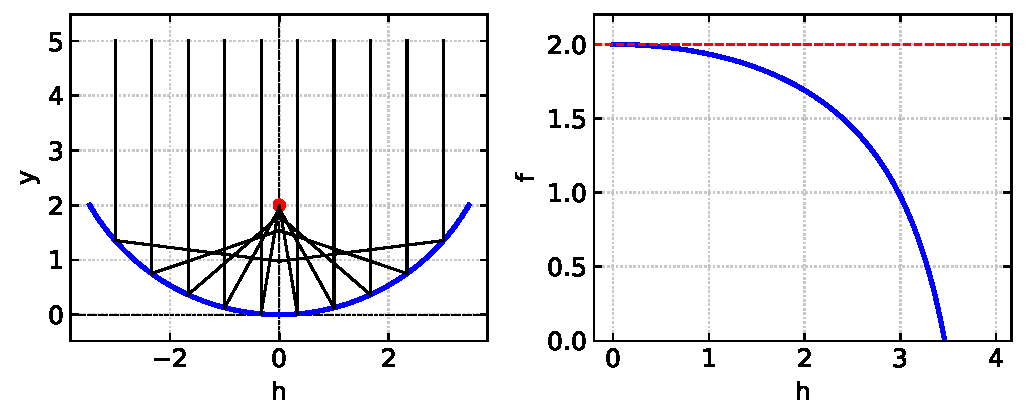
\includegraphics[keepaspectratio]{geometrical-optics/Optical Elements I_files/figure-pdf/fig-spherical-mirror-output-1.pdf}}

}

\caption{\label{fig-spherical-mirror}Spherical mirror of radius \(R=4\)
reflecting parallel rays, showing spherical aberration and focal
distance as a function of the distance from the optical axis \(h\).}

\end{figure}%

\end{tcolorbox}

To obtain now an equation which predicts the point at which the
reflected ray intersects the optical axis if it emerged at a point
\(A\), we just consider the following sketch.

\begin{figure}

\centering{

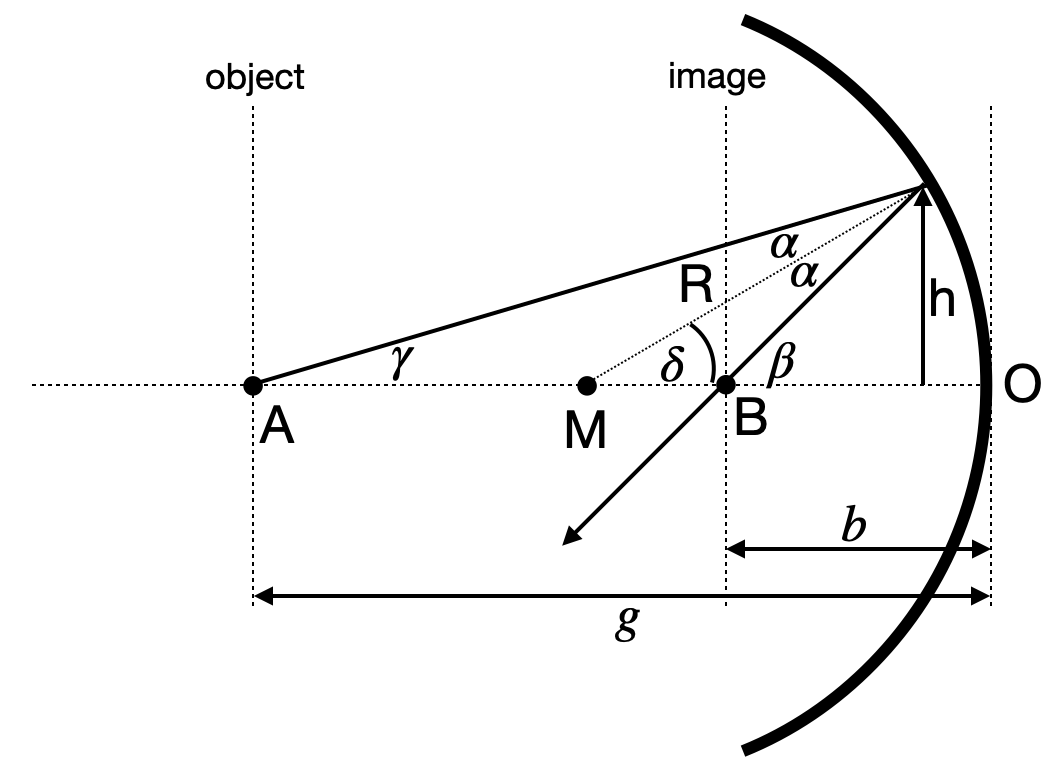
\includegraphics[width=0.6\linewidth,height=\textheight,keepaspectratio]{geometrical-optics/img/image_concave_mirror.png}

}

\caption{\label{fig-concave-mirror}Image formation on a concave mirror.}

\end{figure}%

For this situation, we can write down immediately the following
relations

\[\delta=\alpha+\gamma\]

\[\gamma+\beta=2\delta\]

Further under the assumption of small angles
(\hyperref[paraxial-approximation]{paraxial approximation}) we can write
down

\[\tan(\gamma) \approx \gamma = \frac{h}{g}\]
\[\tan(\beta) \approx \beta = \frac{h}{b}\]
\[\sin(\delta) \approx \delta = \frac{h}{R}\]

from which we obtain

\[\frac{h}{g}+\frac{h}{b}=2\frac{h}{R}\]

and by divding by \(h\) finally the imaging equation:

\[\frac{1}{g}+\frac{1}{b}= \frac{2}{R}= \frac{1}{f}\]

where we have used the focal length \(f=R/2\). This equation has some
surprising property. It is completely independent of \(h\) and
\(\gamma\). That means all points in a plane at a distance \(g\) are
images into a plane at a distance \(b\). Both planes are therefore
called conjugated planes.

\begin{tcolorbox}[enhanced jigsaw, breakable, toptitle=1mm, bottomrule=.15mm, colbacktitle=quarto-callout-note-color!10!white, title=\textcolor{quarto-callout-note-color}{\faInfo}\hspace{0.5em}{Imaging Equation Concave Mirror}, arc=.35mm, rightrule=.15mm, bottomtitle=1mm, opacityback=0, toprule=.15mm, coltitle=black, leftrule=.75mm, opacitybacktitle=0.6, colback=white, left=2mm, titlerule=0mm, colframe=quarto-callout-note-color-frame]

The sum of the inverse object and image distances equals the inverse
focal length of the cocave mirror.

\[\frac{1}{g}+\frac{1}{b}\approx\frac{1}{f}\]

\end{tcolorbox}

This equation now helps to construct the image of an object in front of
a concave mirror and we may define 3 different rays to identify the size
of an image \(h_{\text{image}}\) from the size of an object
\(h_{\text{object}}\).

\begin{figure}

\centering{

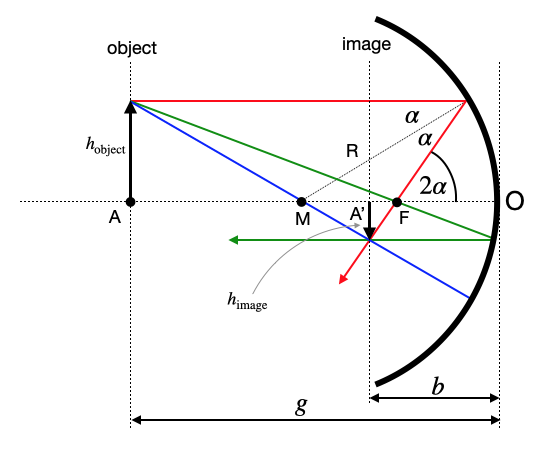
\includegraphics[width=0.6\linewidth,height=\textheight,keepaspectratio]{geometrical-optics/img/image_size.png}

}

\caption{\label{fig-concave-mirror-image}Image formation on a concave
mirror.}

\end{figure}%

In the diagram above, three key rays are used to construct the image:

\begin{enumerate}
\def\labelenumi{\arabic{enumi}.}
\tightlist
\item
  \textbf{Red ray:} Parallel to optical axis → reflects through focal
  point
\item
  \textbf{Green ray:} Through focal point → reflects parallel to optical
  axis
\item
  \textbf{Central ray:} Through center of curvature → reflects back
  along same path
\end{enumerate}

The behavior of these reflected rays determines the nature of the image:

\begin{itemize}
\tightlist
\item
  If the rays intersect on the same side of the mirror as the object, a
  \textbf{real image} forms. This image is inverted, as shown in the
  sketch.
\item
  If the rays diverge after reflection, they appear to intersect behind
  the mirror, creating a \textbf{virtual image}. This image is upright
  and located behind the mirror, though no actual ray intersection
  occurs.
\end{itemize}

The point where these rays meet (or appear to meet) determines the image
size. By drawing a ray from the object's tip through the mirror's center
(point O), we can easily determine the image height h\_image. As an
exercise, consider how this construction demonstrates that the
magnification of a concave mirror is given by

\[ \frac{h_{\text{image}}}{h_{\text{object}}}=-\frac{b}{g}=M\]

This ratio indeed represents the magnification \(M\). The negative sign
in the expression reflects an important optical property: for real
images formed by concave mirrors, the image is inverted relative to the
object. This inversion is mathematically represented by the negative
magnification value. Conversely, a positive magnification would indicate
an upright image, which occurs with virtual images.

With the help of the imaging equation and the magnification we may in
general differentiate between the following general situations:

\begin{longtable}[]{@{}
  >{\raggedright\arraybackslash}p{(\linewidth - 6\tabcolsep) * \real{0.2394}}
  >{\raggedright\arraybackslash}p{(\linewidth - 6\tabcolsep) * \real{0.3099}}
  >{\raggedright\arraybackslash}p{(\linewidth - 6\tabcolsep) * \real{0.2394}}
  >{\raggedright\arraybackslash}p{(\linewidth - 6\tabcolsep) * \real{0.2113}}@{}}
\toprule\noalign{}
\begin{minipage}[b]{\linewidth}\raggedright
Object Distance
\end{minipage} & \begin{minipage}[b]{\linewidth}\raggedright
Image Characteristics
\end{minipage} & \begin{minipage}[b]{\linewidth}\raggedright
Image Position
\end{minipage} & \begin{minipage}[b]{\linewidth}\raggedright
Magnification
\end{minipage} \\
\midrule\noalign{}
\endhead
\bottomrule\noalign{}
\endlastfoot
\(g > 2f\) & Real, inverted, smaller & Between f and 2f & \(|m|\)
\textless{} 1 \\
\(g = 2f\) & Real, inverted, same size & At 2f & \(|m|\) = 1 \\
\(f < g < 2f\) & Real, inverted, larger & Beyond 2f & \(|m|\)
\textgreater{} 1 \\
\(g = f\) & Image at infinity & At infinity & N/A \\
\(g < f\) & Virtual, upright, larger & Behind mirror & \(|m|\)
\textgreater{} 1 \\
\end{longtable}

\begin{tcolorbox}[enhanced jigsaw, breakable, toptitle=1mm, bottomrule=.15mm, colbacktitle=quarto-callout-note-color!10!white, title=\textcolor{quarto-callout-note-color}{\faInfo}\hspace{0.5em}{Parabolic Mirrors Focus Parallel Rays}, arc=.35mm, rightrule=.15mm, bottomtitle=1mm, opacityback=0, toprule=.15mm, coltitle=black, leftrule=.75mm, opacitybacktitle=0.6, colback=white, left=2mm, titlerule=0mm, colframe=quarto-callout-note-color-frame]

We would like to show in the following, that a parabolic mirror is a
shape which reflects all light rays parallel to the principal axis to a
single point, the focus. This is a fundamental property of parabolic
mirrors and is used in many optical systems, such as telescopes,
satellite dishes, and car headlights.

For this purpose, we would like to use Fermat's principle. We examine a
light ray originating from a point \(x,y_0\) and travelling parallel to
the principal axis. The light ray is reflected at a point \((x,y)\) on
the mirror and travels to the focus at \((0,p)\). The light path is
therefore consisting out of two linear segments \(A\) and \(B\) for
which we have to calculate the time of travel. The total duration of the
light's journey is then: \[
t = t_A + t_B
\]

where:

\begin{itemize}
\tightlist
\item
  \(t_A\) is the time taken to travel from \(x,y_0\) to the mirror.
\item
  \(t_B\) is the time taken to travel from \((x,y)\) to \((0,p)\).
\end{itemize}

\subsubsection{Time for Path A}\label{time-for-path-a}

The distance covered in path A is equal to \(y_0 - y\), where \(y\)
represents the y-coordinate of the point where the ray meets the mirror.
Consequently, the time taken for the light to traverse path A can be
expressed as:

\[
t_A = \frac{y_0 - y}{c}
\]

In this equation, \(c\) represents the speed of light in the medium.

\subsubsection{Time for Path B}\label{time-for-path-b}

After reflection, the light ray travels from the point \((x, y)\) on the
mirror's surface to the focal point located at \((0, p)\). The length of
this segment of the path can be calculated using the distance formula:

\[
\sqrt{x^2 + (y - p)^2}
\]

Consequently, the time required for the light to traverse path B is
expressed as:

\[
t_B = \frac{\sqrt{x^2 + (y - p)^2}}{c}
\]

\subsubsection{Total Time}\label{total-time}

The total time for the light ray's journey is the sum of times for paths
A and B:

\[
t = \frac{y_0 - y}{v} + \frac{\sqrt{x^2 + (y - p)^2}}{c}
\]

According to Fermat's principle, all light rays should take the same
time. We can express this by setting the total time equal to a constant
\(t_c\):

\[
\frac{y_0 - y}{v} + \frac{\sqrt{x^2 + (y - p)^2}}{v} = t_c
\]

For a ray traveling along the y-axis, reflecting at \((0, 0)\), the
total distance is \(y_0 + p\). The time for this ray is:

\[
\frac{y_0 + p}{c}
\]

This gives us \(t_c = \frac{y_0 + p}{c}\). Substituting into our general
equation:

\[
\frac{y_0 - y}{v} + \frac{\sqrt{x^2 + (y - p)^2}}{c} = \frac{y_0 + p}{c}
\]

Multiplying by \(c\) and rearranging:

\[
y_0 - y + \sqrt{x^2 + (y - p)^2} = y_0 + p
\]

\[
\sqrt{x^2 + (y - p)^2} = y + p
\]

Squaring both sides and simplifying:

\[
x^2 + (y - p)^2 = (y + p)^2
\]

\[
x^2 + y^2 - 2py + p^2 = y^2 + 2py + p^2
\]

\[
x^2 = 4py
\]

or

\[
y=\frac{1}{4p}x^2
\]

This final equation describes a parabola with its focus at \((0, p)\).
The code below plots a parabolic mirror reflecting parallel rays to the
focal point. Yet, I'm cheating a bit here. I'm not calculating the
reflected rays, but just plotting them.

\begin{figure}[H]

\centering{

\pandocbounded{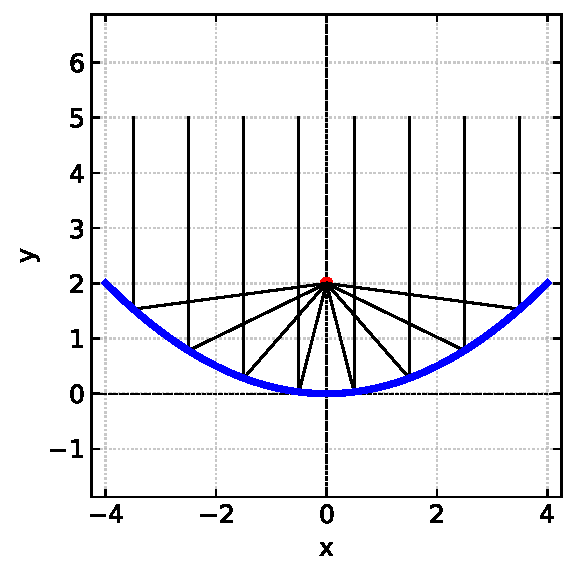
\includegraphics[keepaspectratio]{geometrical-optics/Optical Elements I_files/figure-pdf/fig-parabolic-mirror-output-1.pdf}}

}

\caption{\label{fig-parabolic-mirror}Parabolic mirror reflecting
parallel rays to focal point}

\end{figure}%

\end{tcolorbox}

\begin{tcolorbox}[enhanced jigsaw, breakable, toptitle=1mm, bottomrule=.15mm, colbacktitle=quarto-callout-note-color!10!white, title=\textcolor{quarto-callout-note-color}{\faInfo}\hspace{0.5em}{Elliptical Mirrors and Fermat's Principle}, arc=.35mm, rightrule=.15mm, bottomtitle=1mm, opacityback=0, toprule=.15mm, coltitle=black, leftrule=.75mm, opacitybacktitle=0.6, colback=white, left=2mm, titlerule=0mm, colframe=quarto-callout-note-color-frame]

There is one interesting feature about elliptical mirrors: they can
focus light from one focal point to the other. This is because the sum
of the distances from any point on the ellipse to the two focal points
is constant. This property is known as the \textbf{ellipse's geometric
definition} and you can try that at home with a piece of string and two
pins.

We can now apply Fermat's principle to proof that the light reflected
from the ellipse travels a path length that is a saddle point. This
means that the path length is stationary with respect to small
perturbations in the path. Assuming for example that light travels from
one focal point by a different path that is reflected from a line which
is tangent to the ellipse at the point of reflection, the path length
would be longer at any other point than the initial reflection point.

On the other side, if we reflect the ray on a surface that is a circle,
which is intersecting the ellipse at the point of reflection, the path
length would be shorter at any other point than the initial reflection
point. This is a proof that the ellipse is a saddle point.

\pandocbounded{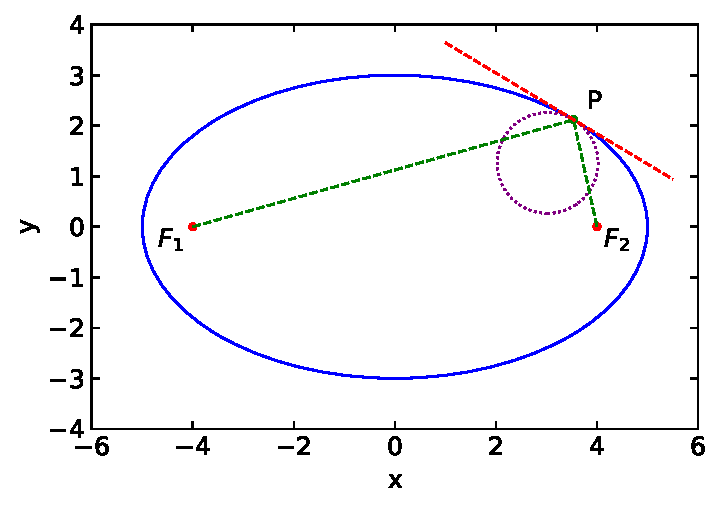
\includegraphics[keepaspectratio]{geometrical-optics/Optical Elements I_files/figure-pdf/cell-5-output-1.pdf}}

\subsubsection{Mathematical Description}\label{mathematical-description}

\subsubsection{Ellipse Definition}\label{ellipse-definition}

Consider an ellipse with semi-major axis \(a\) and semi-minor axis
\(b\), defined by:

\[\frac{x^2}{a^2} + \frac{y^2}{b^2} = 1\]

\paragraph{Focal Points}\label{focal-points}

The focal points are located at \(F_1(-c, 0)\) and \(F_2(c, 0)\), where:

\[c^2 = a^2 - b^2\]

\paragraph{Path Length}\label{path-length}

Let \(P(x_0, y_0)\) be a point on the ellipse. The total path length
\(L\) from \(F_1\) to \(F_2\) via \(P\) is:

\[L = |F_1P| + |PF_2| = \sqrt{(x_0+c)^2 + y_0^2} + \sqrt{(x_0-c)^2 + y_0^2}\]

\paragraph{Fermat's Principle}\label{fermats-principle-1}

The path length \(L\) is stationary with respect to small perturbations
in \(P\):

\[\frac{\partial L}{\partial x_0} = 0 \quad \text{and} \quad \frac{\partial L}{\partial y_0} = 0 \quad \text{at the reflection point}\]

\paragraph{Tangent Line}\label{tangent-line}

The tangent line to the ellipse at \(P(x_0, y_0)\) is given by:

\[\frac{x_0x}{a^2} + \frac{y_0y}{b^2} = 1\]

Let \(Q\) be any point on this tangent line different from \(P\). The
path \(F_1 \to Q \to F_2\) is longer than \(F_1 \to P \to F_2\):

\[|F_1Q| + |QF_2| > |F_1P| + |PF_2|\]

\paragraph{Circle of Curvature}\label{circle-of-curvature}

The radius of curvature \(R\) at \(P\) is:

\[R = \frac{(a^2b^2)^{3/2}}{(b^2x_0^2 + a^2y_0^2)^{3/2}}\]

The center of curvature \(C\) is located at:

\[C = P + R\cdot\mathbf{n}\]

where \(\mathbf{n}\) is the unit normal vector at \(P\).

Let \(Q\) be any point on this circle different from \(P\). The path
\(F_1 \to Q \to F_2\) is shorter than \(F_1 \to P \to F_2\):

\[|F_1Q| + |QF_2| < |F_1P| + |PF_2|\]

As a consequence, the path length for the reflection on and ellipse
between the two focal points must be a saddle point.

\end{tcolorbox}

\chapter{Optical Elements Part II}\label{optical-elements-part-ii}

\section{Prism}\label{prism}

Prisms are wedge-shaped optical elements made of a transparent material,
such as glass. A special form of such a prism is an isosceles prism with
two sides of equal length. The two equal sides enclose an angle
\(\gamma\), known as the apex angle of the prism. When light passes
through this prism, it undergoes refraction twice.

First, the incident angle \(\alpha_1\) is changed into a refracted angle
\(\beta_1\) as the light enters the prism. This refracted ray then hits
the second interface at an angle \(\beta_2\), leading to a second
refraction as it exits the prism at an angle \(\alpha_2\).

Of particular interest is the total deflection of the incident ray,
which is measured by the angle \(\delta\). This deflection angle
represents the difference between the final outgoing angle \(\alpha_2\)
and the initial incident angle \(\alpha_1\).

Understanding how this deflection angle changes based on the prism's
properties and the incident angle is crucial in various optical
applications. In the following sections, we will explore how to
calculate this deflection angle and examine its dependence on different
parameters.

\begin{figure}

\centering{

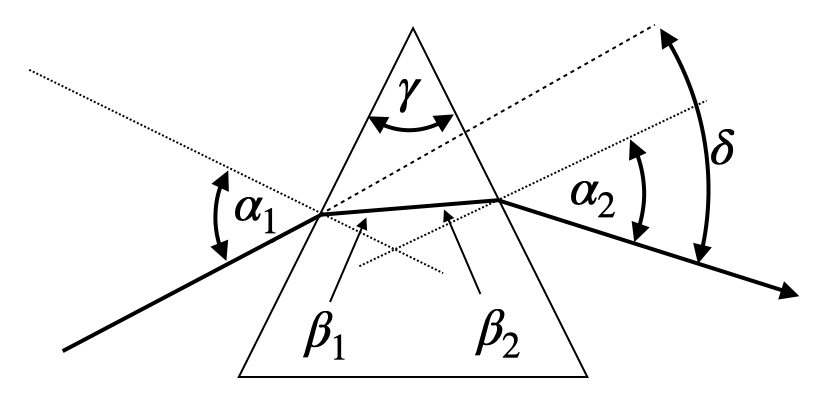
\includegraphics[width=0.4\linewidth,height=\textheight,keepaspectratio]{geometrical-optics/img/prism.png}

}

\caption{\label{fig-prism}Refraction of rays on a prism.}

\end{figure}%

\subsection{Deflection angle}\label{deflection-angle}

We can calculate the deflection angle \(\delta\) from a number of
considerations. First consider the following relations between the
angles in the prism and Snell's law

\[\beta_1=\sin^{-1}\left (\frac{n_0}{n_1}\sin(\alpha_1) \right)\]
\[\beta_2=\gamma-\beta_1\]
\[\alpha_2=\sin^{-1}\left (\frac{n_1}{n_0}\sin(\beta_2)\right )\]
\[\theta_2=\alpha_2-\gamma\]

where \(\theta_2\) is the angle between the incident surface normal and
the outgoing ray. The total deflection angle \(\delta\) is then

\[\delta =\alpha_1-\beta_1+\alpha_2-\beta_2\]

or

\[\delta =\alpha_1+\alpha_2-\gamma\]

from which we obtain

\[\delta=\alpha_1+\sin^{-1}\left (\frac{n_1}{n_0}\sin\left [\gamma-\sin^{-1}\left (\frac{n_0}{n_1}\sin(\alpha_1) \right)\right]\right )-\gamma\]

as the deflection angle.

\begin{figure}

\centering{

\pandocbounded{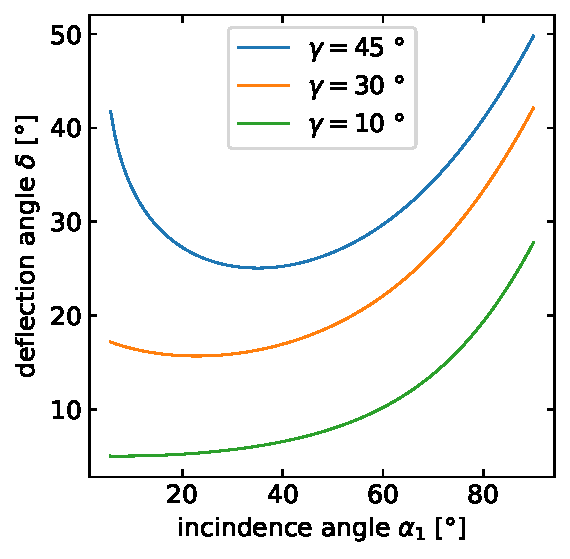
\includegraphics[keepaspectratio]{geometrical-optics/Optical Elements II_files/figure-pdf/fig-refractive-indices-output-1.pdf}}

}

\caption{\label{fig-refractive-indices}Deflection angle as a function of
the incidence angle for different prism angles.}

\end{figure}%

\subsection{Minimum deflection angle}\label{minimum-deflection-angle}

If we now would like to know how the deflection angle changes with the
incident angle \(\alpha_1\), we calculate the derivative of the
deflection angle \(\delta\) with respect to \(\alpha_1\), i.e.,

\[\frac{\mathrm d\delta}{\mathrm d\alpha_1}=1+\frac{\mathrm d\alpha_2}{\mathrm d \alpha_1}.\]

We are here especially interested in the case, where this change in
deflection is reaching a minimum, i.e.,
\(\mathrm d\delta/\mathrm d\alpha_1 =0\). This readily yields

\[\mathrm d \alpha_2=-\mathrm d\alpha_1.\]

This means a change in the incidence angle \(\mathrm d\alpha_1\) yields
an opposite change in the outgoing angle \(-\mathrm d\alpha_2\). We may
later observe that in the experiment.

As both, the incident and the outgoing angle are related to each other
by Snells's law, we may introduce the derivatives of Snell's law for
both interfaces, e.g.,

\begin{itemize}
\tightlist
\item
  \(\cos(\alpha_1)\mathrm d\alpha_1=n\cos(\beta_1)\mathrm d\beta_1\)
\item
  \(\cos(\alpha_2)\mathrm d\alpha_2=n\cos(\beta_2)\mathrm d\beta_2\)
\end{itemize}

where \(n\) is the refractive index of the prism material and the
material outside is air (\(n_{\rm air}=1\)). Replacing
\(\cos(\alpha)=\sqrt{1-\sin^2(\alpha)}\) and dividing the two previous
equations by each other readily yields

\[\frac{1-\sin^2(\alpha_1)}{1-\sin^2(\alpha_2)}=\frac{n^2-\sin^2(\alpha_1)}{n^2-\sin^2(\alpha_2)}.\]

The latter equation is for \(n\neq 1\) only satisfied if
\(\alpha_1=\alpha_2=\alpha\). In this case, the light path through the
prism must be symmetric and we may write down the minimum deflection
angle \(\delta_{\rm min}\):

\begin{tcolorbox}[enhanced jigsaw, breakable, toptitle=1mm, bottomrule=.15mm, colbacktitle=quarto-callout-note-color!10!white, title=\textcolor{quarto-callout-note-color}{\faInfo}\hspace{0.5em}{Minimum prism deflection}, arc=.35mm, rightrule=.15mm, bottomtitle=1mm, opacityback=0, toprule=.15mm, coltitle=black, leftrule=.75mm, opacitybacktitle=0.6, colback=white, left=2mm, titlerule=0mm, colframe=quarto-callout-note-color-frame]

The minimum deflection angle of an isosceles prism with a prism angle
\(\gamma\) is given by

\[\delta_{\rm min}=2\alpha-\gamma.\]

\end{tcolorbox}

Given this minimum deflection angle \(\delta_{\rm min}\) and the
properties of the prism, we may also write down Snell's law using
\(\sin(\alpha)=n\sin(\beta)\), which results in

\[\sin \left ( \frac{\delta_{\rm min}+\gamma}{2}\right )=n\sin\left (\frac{\gamma}{2}\right).\]

which indicates the dependence of the deflection in the refractive index
\(n\) of the prism material.

\subsection{Dispersion}\label{dispersion}

Very important applications now arise from the fact, that the refractive
index is a material property, which depends on the color (frequency or
wavelength) of light. We do not yet understand the origin of this
dependence. The plots below show the wavelength dependence of three
different glasses. You may find much more data on the refractive index
of different materials in an \href{https://refractiveindex.info/}{online
database}.

\begin{figure}

\centering{

\pandocbounded{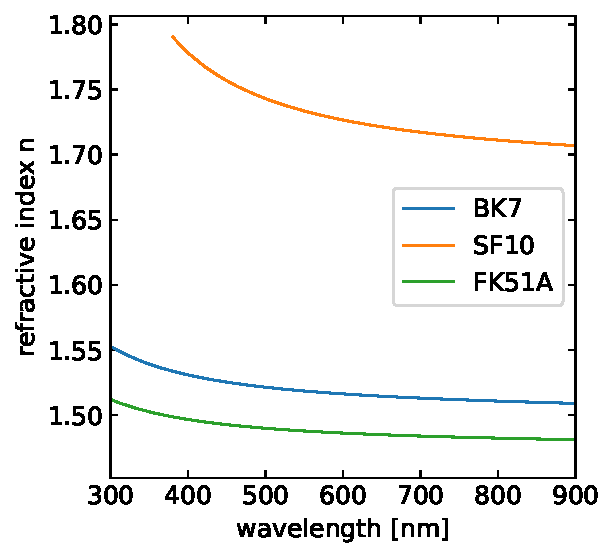
\includegraphics[keepaspectratio]{geometrical-optics/Optical Elements II_files/figure-pdf/fig-wavelength-dependence-output-1.pdf}}

}

\caption{\label{fig-wavelength-dependence}Refractive index of different
glasses as a function of the wavelength.}

\end{figure}%

\begin{figure}

\centering{

\pandocbounded{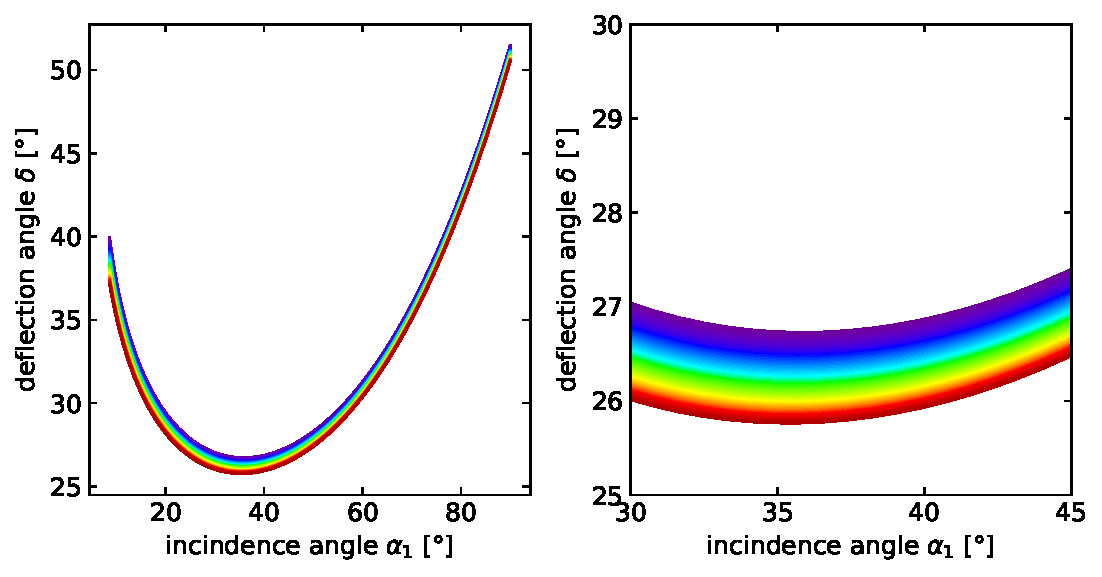
\includegraphics[keepaspectratio]{geometrical-optics/Optical Elements II_files/figure-pdf/fig-angle-dependence-output-1.pdf}}

}

\caption{\label{fig-angle-dependence}Deflection angle as a function of
the incidence angle for different wavelengths.}

\end{figure}%

The plots have a general feature, which is that the refractive index is
largest at small wavelength (blue colors), while it drops continuously
with increasing wavelength towards the red (800 nm). If you would
characterize the dependence by the slope, i.e.,
\(\mathrm dn/\mathrm d\lambda\) then all displayed curves show in the
visible range

\begin{itemize}
\tightlist
\item
  \(\frac{\mathrm dn}{\mathrm d\lambda}<0\), is called normal dispersion
\end{itemize}

while

\begin{itemize}
\tightlist
\item
  \(\frac{\mathrm dn}{\mathrm d\lambda}>0\), is called anomalous
  dispersion
\end{itemize}

This wavelength dependence of the refractive index will yield a
dependence of the deflection angle on the color of light as well. The
change of the deflection angle with the refractive index can be
calculated to be

\[\frac{\mathrm d\delta}{\mathrm d n}=\frac{2\sin(\gamma/2)}{\sqrt{1-n^2\sin^2(\gamma/2)}}\]

together with the relation

\[\frac{\mathrm d \delta}{\mathrm d \lambda}=\frac{\mathrm d\delta}{\mathrm d n}\frac{\mathrm d n}{\mathrm d\lambda}\]

we obtain

\[\frac{\mathrm d\delta}{\mathrm d\lambda}=\frac{2\sin(\gamma/2)}{\sqrt{1-n^2\sin^2(\gamma/2)}}\frac{\mathrm d n}{\mathrm d \lambda}.\]

The refraction of white light through a prism splits the different
colors composing white light spatially into a colored spectrum. In this
process, light with the longest wavelength (red) is deflected the least,
while light with the shortest wavelength (violet) is deflected the most.
This occurs because the refractive index of the prism material varies
with wavelength, a phenomenon known as dispersion.

\begin{figure}

\centering{

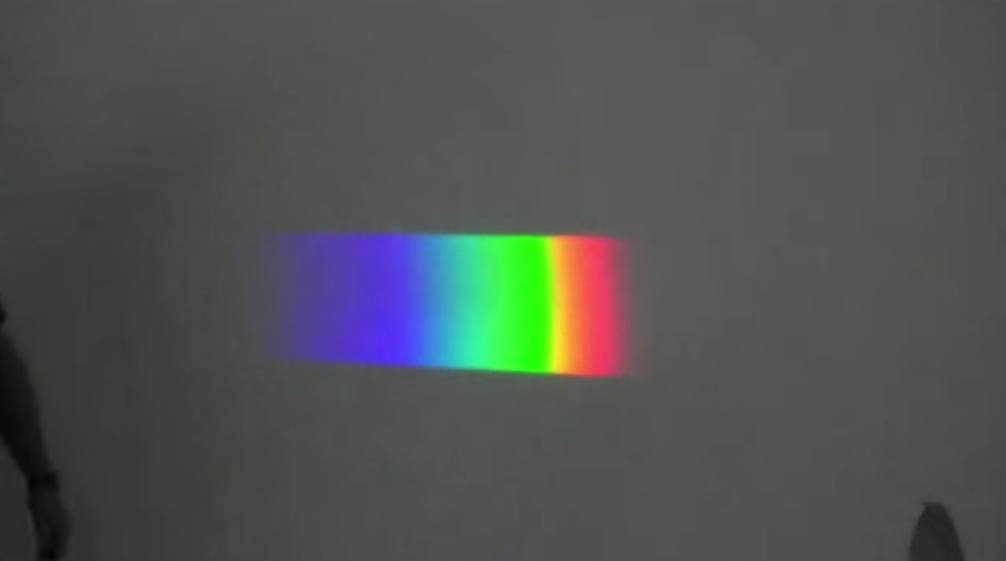
\includegraphics[width=0.49\linewidth,height=\textheight,keepaspectratio]{geometrical-optics/expimg/spectrum.png}

}

\caption{\label{fig-spectrum}Spectrum as created by a prism in the
lecture.}

\end{figure}%

\begin{figure}

\begin{minipage}{0.50\linewidth}

\centering{

\pandocbounded{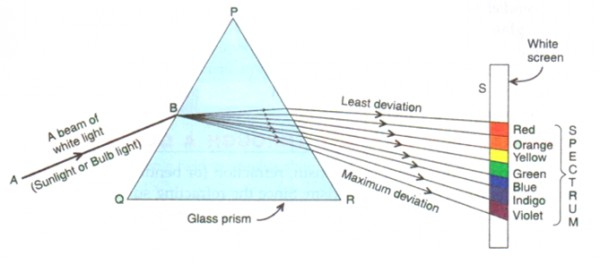
\includegraphics[keepaspectratio]{geometrical-optics/img/spectrum.jpeg}}

}

\subcaption{\label{fig-spectrum}Spectrum}

\end{minipage}%
%
\begin{minipage}{0.50\linewidth}

\centering{

\pandocbounded{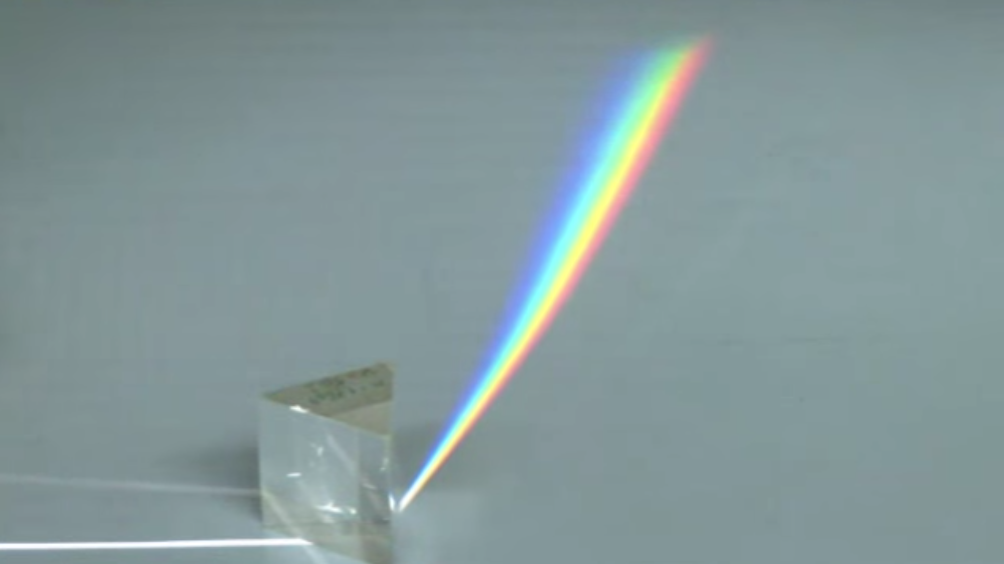
\includegraphics[keepaspectratio]{geometrical-optics/expimg/prism.png}}

}

\subcaption{\label{fig-prism}Prism}

\end{minipage}%

\caption{\label{fig-prism-spectrum}Deflection of different wavelengths
of light in a prism with normal dispersion.}

\end{figure}%

\subsection{Prims spectrograph}\label{prims-spectrograph}

This wavelength-dependent refraction is crucial as it forms the basis
for spectroscopy, a powerful analytical technique that measures and
records the intensity of light as a function of wavelength. Spectroscopy
allows scientists to analyze the composition and properties of matter by
examining its interaction with light across different wavelengths.

\begin{figure}

\begin{minipage}{0.50\linewidth}

\centering{

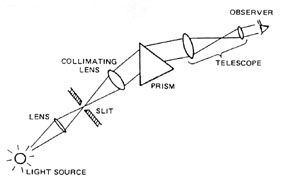
\includegraphics[width=1\linewidth,height=\textheight,keepaspectratio]{geometrical-optics/img/prism_spec_principle.jpeg}

}

\subcaption{\label{fig-spec-principle}Principle of a prism spectrometer}

\end{minipage}%
%
\begin{minipage}{0.50\linewidth}

\centering{

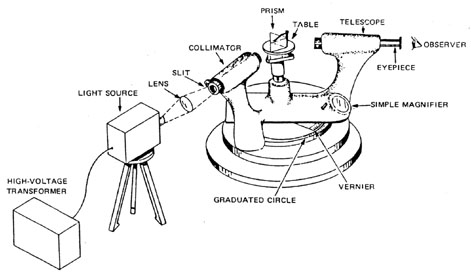
\includegraphics[width=1\linewidth,height=\textheight,keepaspectratio]{geometrical-optics/img/prism_spectrometer.jpeg}

}

\subcaption{\label{fig-spec-realization}Technical realization of a prism
spectrometer}

\end{minipage}%

\caption{\label{fig-prism-spectrometer}Principle and technical
realization of a prism spectrometer.}

\end{figure}%

\textbf{DIY prism}

If you don't have a prism at home (which most people don't), you can
create a simple substitute using a mirror and a basin of water. Here's
how:

\begin{enumerate}
\def\labelenumi{\arabic{enumi}.}
\tightlist
\item
  Place a mirror in a basin of water, partially submerged.
\item
  Shine white light from a flashlight onto the mirror.
\item
  Observe the reflected and refracted light, paying special attention to
  the edges.
\end{enumerate}

For better results, you can create a small aperture by making a tiny
hole in a piece of black paper and placing it in front of the
flashlight.

\begin{figure}

\centering{

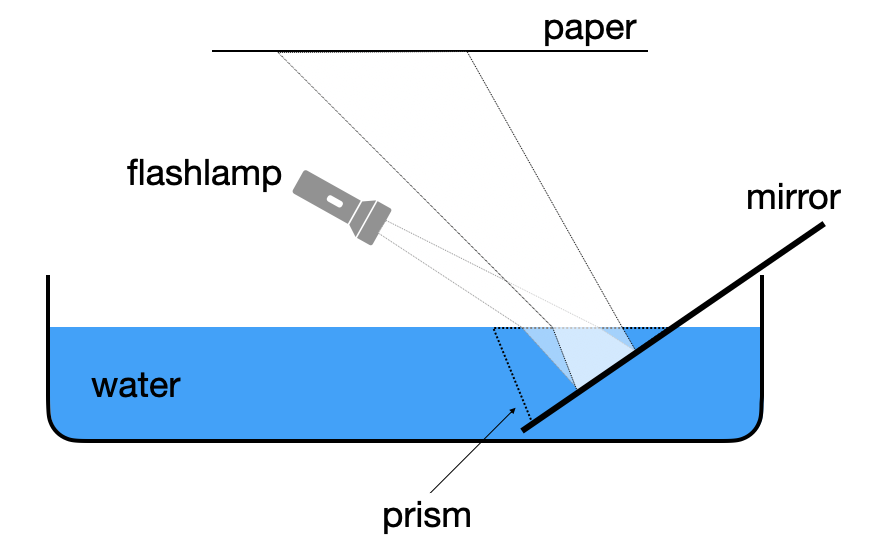
\includegraphics[width=0.6\linewidth,height=\textheight,keepaspectratio]{geometrical-optics/img/diy_prism.png}

}

\caption{\label{fig-diy-prism}Home made water prism.}

\end{figure}%

While the dependence of water's refractive index on wavelength is
relatively weak, it's still sufficient to demonstrate the familiar
colors of the rainbow. This phenomenon will be referenced later in our
discussion.

\begin{figure}

\centering{

\pandocbounded{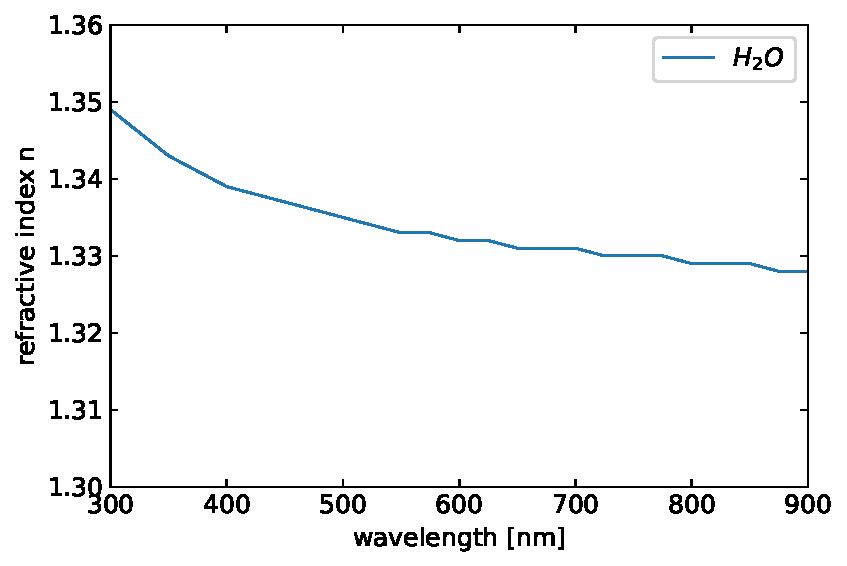
\includegraphics[keepaspectratio]{geometrical-optics/Optical Elements II_files/figure-pdf/fig-water-n-output-1.pdf}}

}

\caption{\label{fig-water-n}Refractive index of water as a function of
the wavelength.}

\end{figure}%

\begin{tcolorbox}[enhanced jigsaw, breakable, toptitle=1mm, bottomrule=.15mm, colbacktitle=quarto-callout-note-color!10!white, title=\textcolor{quarto-callout-note-color}{\faInfo}\hspace{0.5em}{Applications of prims}, arc=.35mm, rightrule=.15mm, bottomtitle=1mm, opacityback=0, toprule=.15mm, coltitle=black, leftrule=.75mm, opacitybacktitle=0.6, colback=white, left=2mm, titlerule=0mm, colframe=quarto-callout-note-color-frame]

Prisms are versatile optical components with a wide range of
applications across various fields. Here are some common uses of prisms:

\subsubsection{Binoculars and
Telescopes:}\label{binoculars-and-telescopes}

Porro prisms in traditional binoculars and roof prisms in modern designs
serve to correct image inversion and provide a compact form. These
prisms enable a longer optical path within a shorter physical length,
enhancing magnification while maintaining portability. This design is
crucial for both binoculars and some telescopes, offering users powerful
magnification in a handheld device.

\subsubsection{Periscopes:}\label{periscopes}

Right-angle prisms are the key component in periscopes, redirecting
light at 90-degree angles. This simple yet effective design allows
viewers to see over obstacles or around corners, making periscopes
invaluable in submarines and various military applications where direct
line of sight is obstructed.

\subsubsection{Beam Splitting:}\label{beam-splitting}

Cube beamsplitters play a vital role in dividing a single beam of light
into two separate beams. This capability is essential in various
scientific and medical applications, including interferometry,
holography, and optical coherence tomography (OCT). The ability to split
light beams precisely opens up numerous possibilities in research and
diagnostics.

\subsubsection{Beam Steering:}\label{beam-steering}

Risley prisms, consisting of a pair of rotating wedge prisms, offer
precise control over laser beam direction. This technology finds
applications in laser scanning, target tracking, and adaptive optics.
The ability to steer beams accurately is crucial in fields ranging from
military applications to advanced scientific research.

\subsubsection{Digital Projectors:}\label{digital-projectors}

Total Internal Reflection (TIR) prisms are a crucial component in
Digital Light Processing (DLP) projectors. They direct light from the
lamp to the Digital Micromirror Device (DMD) and then to the projection
lens, enabling the high-quality image projection that DLP technology is
known for.

\subsubsection{Camera Systems:}\label{camera-systems}

In Single-Lens Reflex (SLR) cameras, pentaprisms play a critical role in
the viewfinder system. They flip the image from the lens to appear
upright and correctly oriented in the viewfinder, allowing photographers
to accurately compose their shots.

\subsubsection{Laser Systems:}\label{laser-systems}

Brewster prisms find use in laser systems for polarization and
wavelength separation. Additionally, dispersing prisms can be employed
for wavelength tuning in certain laser setups, providing precise control
over the laser's output characteristics.

\subsubsection{Fiber Optic
Communications:}\label{fiber-optic-communications}

In the realm of telecommunications, prisms are utilized in some fiber
optic connectors and switches. They help redirect light between fibers,
playing a crucial role in maintaining signal integrity and enabling
complex network architectures.

\subsubsection{Solar Energy:}\label{solar-energy}

Fresnel lenses, a specialized type of prism, are employed in
concentrated solar power systems. These lenses focus sunlight
efficiently, contributing to the development of more effective solar
energy collection technologies.

\subsubsection{Head-Up Displays (HUDs):}\label{head-up-displays-huds}

Prisms are an integral part of HUD systems in both automotive and
aviation contexts. They project crucial information onto the windshield
or a combiner glass, allowing drivers or pilots to access important data
without taking their eyes off their primary viewpoint.

\subsubsection{Microscopy:}\label{microscopy}

Nomarski prisms enhance the capabilities of differential interference
contrast microscopy. They increase contrast in transparent specimens,
enabling scientists to observe details that would be difficult or
impossible to see with conventional microscopy techniques.

\subsubsection{Optical Coherence Tomography
(OCT):}\label{optical-coherence-tomography-oct}

In some OCT systems, prisms are employed for sample arm scanning and
reference arm delay. This application of prisms contributes to the
high-resolution imaging capabilities of OCT, which is particularly
valuable in medical diagnostics, especially in ophthalmology.

\end{tcolorbox}

\chapter{Optical Elements Part III}\label{optical-elements-part-iii}

\subsection{Lenses}\label{lenses}

The most important optical elements are lenses, which come in many
different flavors. They consist of curved surfaces, which most commonly
have the shape of a part of a spherical cap. It is, therefore, useful to
have a look at the refraction at spherical surfaces.

\subsubsection{Refraction at spherical
surfaces}\label{refraction-at-spherical-surfaces}

For our calculations of the refraction at spherical surfaces, we
consider the sketch below.

\begin{figure}

\centering{

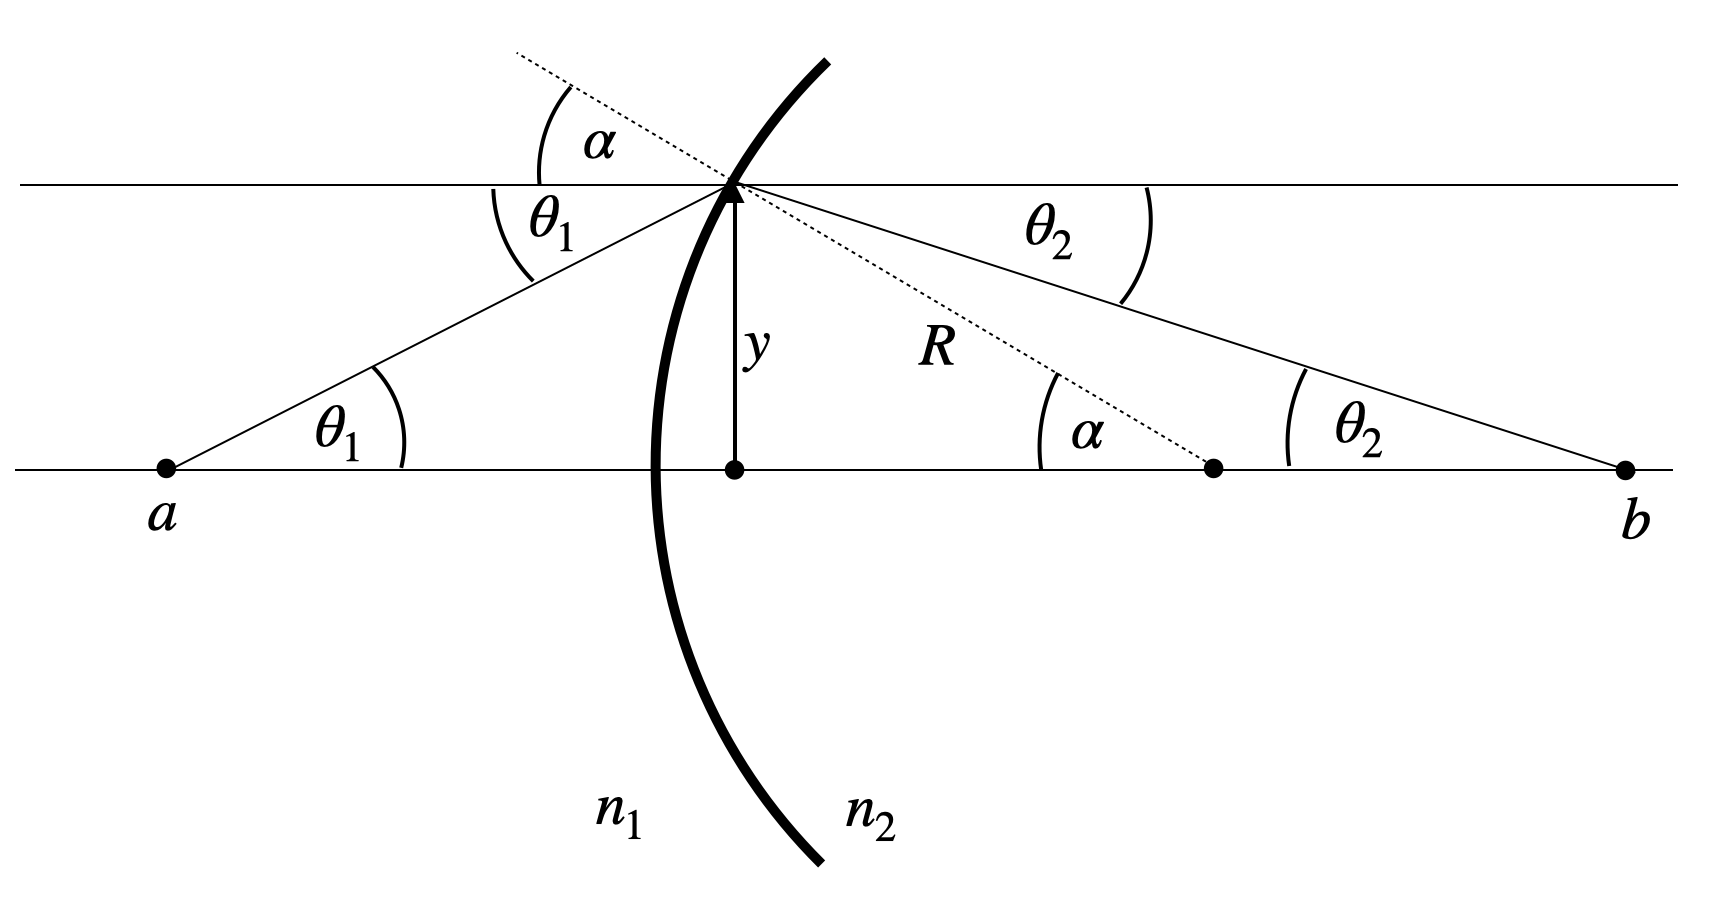
\includegraphics[width=0.8\linewidth,height=\textheight,keepaspectratio]{geometrical-optics/img/curved_surface.png}

}

\caption{\label{fig-curved-surface}Refraction at a curved surface.}

\end{figure}%

To derive an imaging equation for a lens, we aim to calculate the
distance \(b\) and angle \(\theta_2\) at which a ray crosses the optical
axis, given its origin at distance \(a\) and angle \(\theta_1\). We
begin with Snell's law for the geometry:

\[n_{1}\sin(\alpha+\theta_1)=n_{2}\sin(\alpha-\theta_2)\]

We define key relationships:

\[\sin(\alpha)=\frac{y}{R}, \quad \tan(\theta_1)=\frac{y}{a}, \quad \tan(\theta_2)=\frac{y}{b}\]

To simplify this, we employ the \textbf{paraxial approximation}, which
assumes all angles are small. This allows us to use first-order
approximations of trigonometric functions, effectively linearizing them:

\[\sin(\theta) \approx \theta+ O(\theta^{3}), \quad \tan(\theta) \approx \theta + O(\theta^{3}),\quad \cos(\theta)\approx 1 + O(\theta^{2})\]

This approach, common in optics, significantly simplifies our
calculations while maintaining accuracy for most practical scenarios
involving lenses.

With the help of these approximations we can write Snell's law for the
curved surface as

\[n_1(\alpha+\theta_1)=n_2(\alpha-\theta_2).\]

With some slight transformation which you will find in the video of the
online lecture we obtain, therefore,

\[\theta_2=\frac{n_2-n_1}{n_2 R}y -\frac{n_1}{n_2}\theta_1,\]

which is a purely linear equation in \(y\) and \(\theta_1\).

\begin{tcolorbox}[enhanced jigsaw, breakable, toptitle=1mm, bottomrule=.15mm, colbacktitle=quarto-callout-note-color!10!white, title=\textcolor{quarto-callout-note-color}{\faInfo}\hspace{0.5em}{Paraxial Approximation}, arc=.35mm, rightrule=.15mm, bottomtitle=1mm, opacityback=0, toprule=.15mm, coltitle=black, leftrule=.75mm, opacitybacktitle=0.6, colback=white, left=2mm, titlerule=0mm, colframe=quarto-callout-note-color-frame]

The paraxial approximation is a fundamental simplification in optics
that assumes all angles are small. This allows us to use linear
approximations for trigonometric functions, significantly simplifying
calculations while maintaining accuracy for most practical scenarios
involving lenses.

To visualize the validity of this approximation, let's examine two
plots:

\begin{enumerate}
\def\labelenumi{\arabic{enumi}.}
\tightlist
\item
  The first plot compares sin(θ) (blue line) with its linear
  approximation θ (red dashed line) for angles ranging from 0 to π/2
  radians.
\item
  The second plot shows the absolute error between sin(θ) and θ.
\end{enumerate}

These plots demonstrate that:

\begin{enumerate}
\def\labelenumi{\arabic{enumi}.}
\tightlist
\item
  For small angles (roughly up to 0.5 radians or about 30 degrees), the
  approximation is very close to the actual sine function.
\item
  The error increases rapidly for larger angles, indicating the
  limitations of the paraxial approximation.
\end{enumerate}

In most optical systems, especially those involving lenses, the angles
of incident and refracted rays are typically small enough for this
approximation to be valid. However, it's important to be aware of its
limitations when dealing with wide-angle optical systems or scenarios
where precision is critical.

\begin{figure}[H]

{\centering \pandocbounded{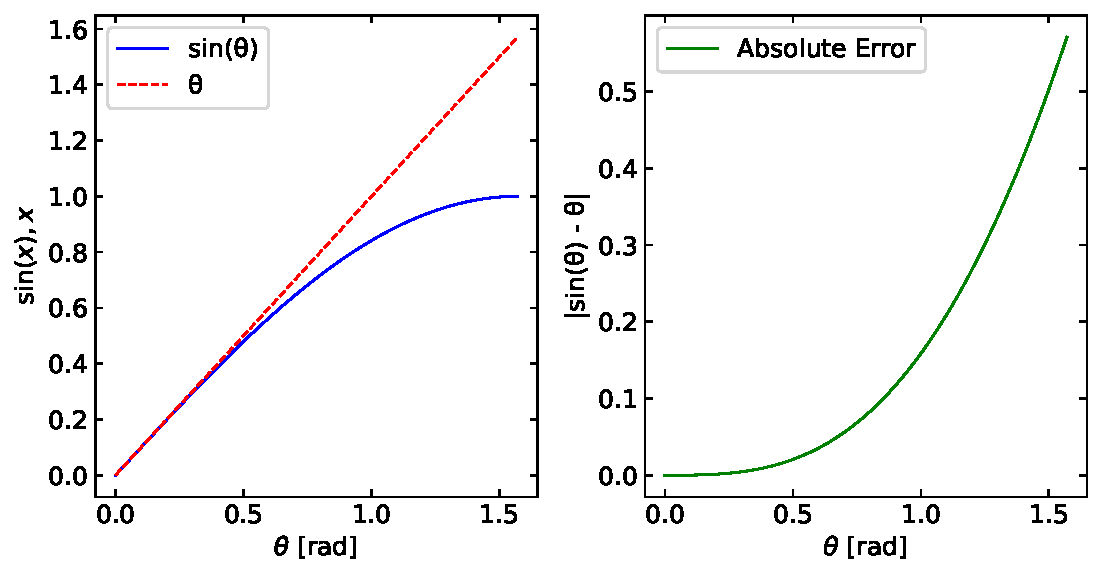
\includegraphics[keepaspectratio]{geometrical-optics/Optical Elements III_files/figure-pdf/cell-3-output-1.pdf}}

}

\caption{Visualization of the paraxial approximation plotting the
\(\sin(\theta)\) and the linear approximation \(\theta\) (dashed line)
for angles ranging from 0 to \(\pi/2\) radians.}

\end{figure}%

\end{tcolorbox}

Consider light originating from a point at distance \(y\) from the
optical axis. We'll analyze two rays: one traveling parallel to the
optical axis and hitting the spherical surface at height \(y\), and
another incident at \(y=0\).

\begin{figure}

\centering{

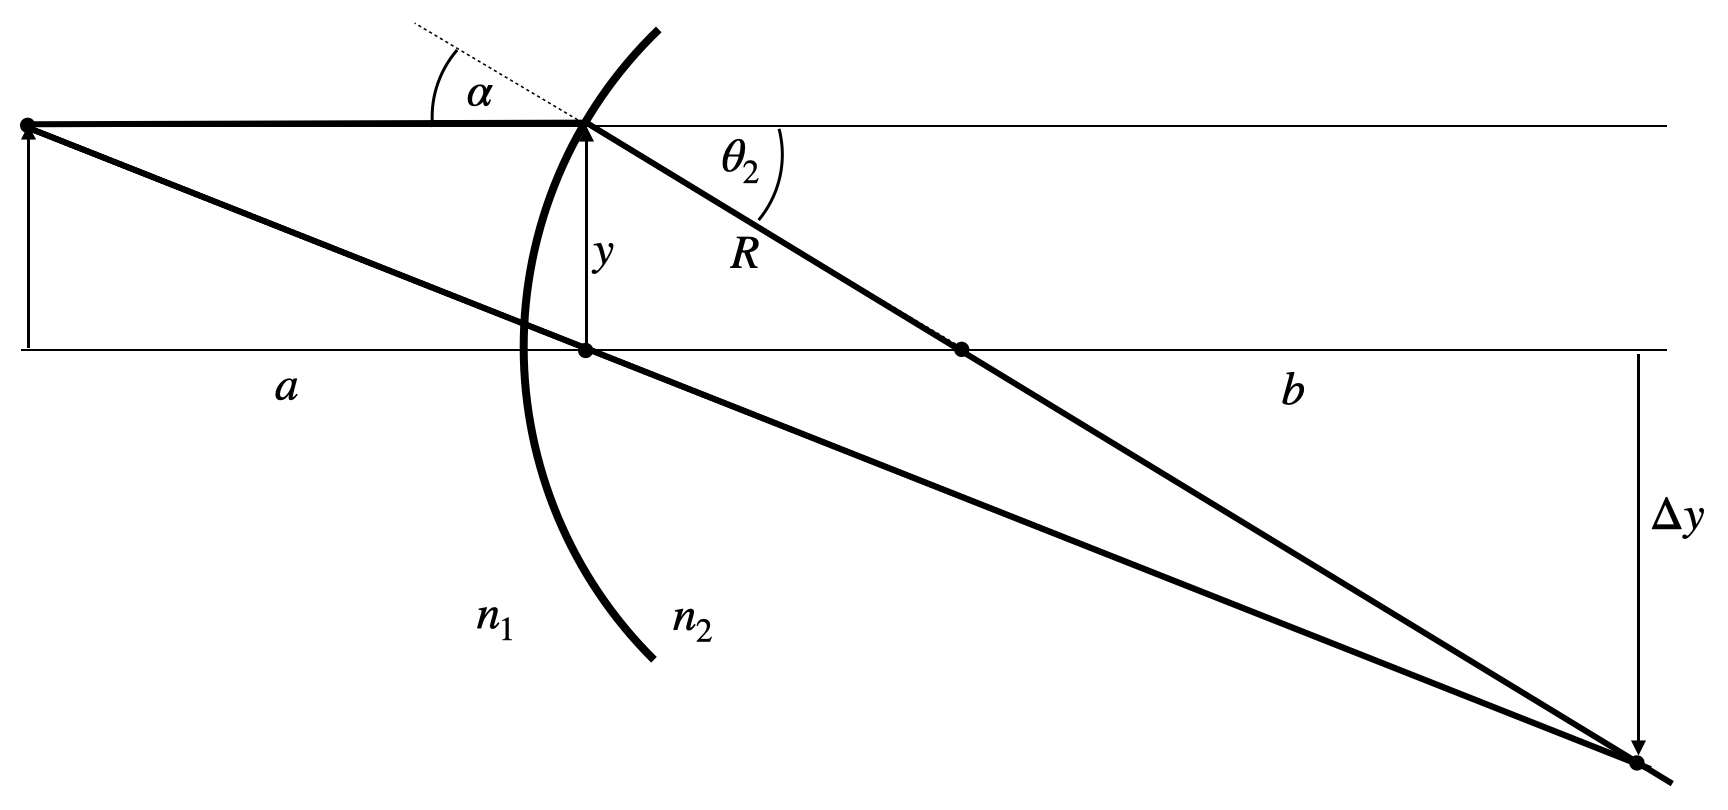
\includegraphics[width=0.8\linewidth,height=\textheight,keepaspectratio]{geometrical-optics/img/image_curved.png}

}

\caption{\label{fig-image-curved}Image formation at a curved surface.}

\end{figure}%

Applying our derived formula to these two cases:

For the parallel ray (\(\theta_1=0\)):

\[\theta_2=\frac{n_2-n_1}{n_2}\frac{y}{R}\]
\[\theta_2=\frac{y+\Delta y}{b}\]

Equating these expressions:

\[\frac{y+\Delta y}{b}=\frac{n_2-n_1}{n_2}\frac{y}{R}\]

For the ray through the center (\(y=0\)):

\[n_2\frac{\Delta y}{b}=n_1\frac{y}{a}\]

Combining these equations yields the imaging equation for a curved
surface:

\[\frac{n_1}{a}+\frac{n_2}{b}=\frac{n_2-n_1}{R}\]

We can define a new quantity, the \textbf{focal length}, which depends
only on the properties of the curved surface:

\[f=\frac{n_2}{n_2-n_1}R\]

\begin{tcolorbox}[enhanced jigsaw, breakable, toptitle=1mm, bottomrule=.15mm, colbacktitle=quarto-callout-note-color!10!white, title=\textcolor{quarto-callout-note-color}{\faInfo}\hspace{0.5em}{Imaging Equation for Spherical Refracting Surface}, arc=.35mm, rightrule=.15mm, bottomtitle=1mm, opacityback=0, toprule=.15mm, coltitle=black, leftrule=.75mm, opacitybacktitle=0.6, colback=white, left=2mm, titlerule=0mm, colframe=quarto-callout-note-color-frame]

The sum of the inverse object and image distances equals the inverse
focal length of the spherical refracting surface:

\[\frac{n_1}{a}+\frac{n_2}{b}\approx\frac{n_2}{f}\]

where the focal length of the refracting surface is given by:

\[f=\frac{n_2}{n_2-n_1}R\]

in the paraxial approximation.

\end{tcolorbox}

\subsection{Thin lens}\label{thin-lens}

In our previous calculation we have found a linear relation between the
incident angle \(\theta_1\) with the optical axis, the incident height
of the ray \(y\) and the outgoing angle \(\theta_2\):

Analyzing refraction in a lens involves two spherical surfaces. Light
initially travels from a medium with refractive index \(n_1\) into the
lens material with index \(n_2\). The first surface's radius, \(R_1\),
is typically positive for a convex surface facing the incident light.

At the second surface, the outgoing angle from the first refraction
becomes the incident angle for the second refraction. Here, light
travels from \(n_2\) back into \(n_1\). The radius \(R_2\) of this
surface often has a negative value in a converging lens due to its
opposite curvature relative to the optical axis.

\begin{figure}

\centering{

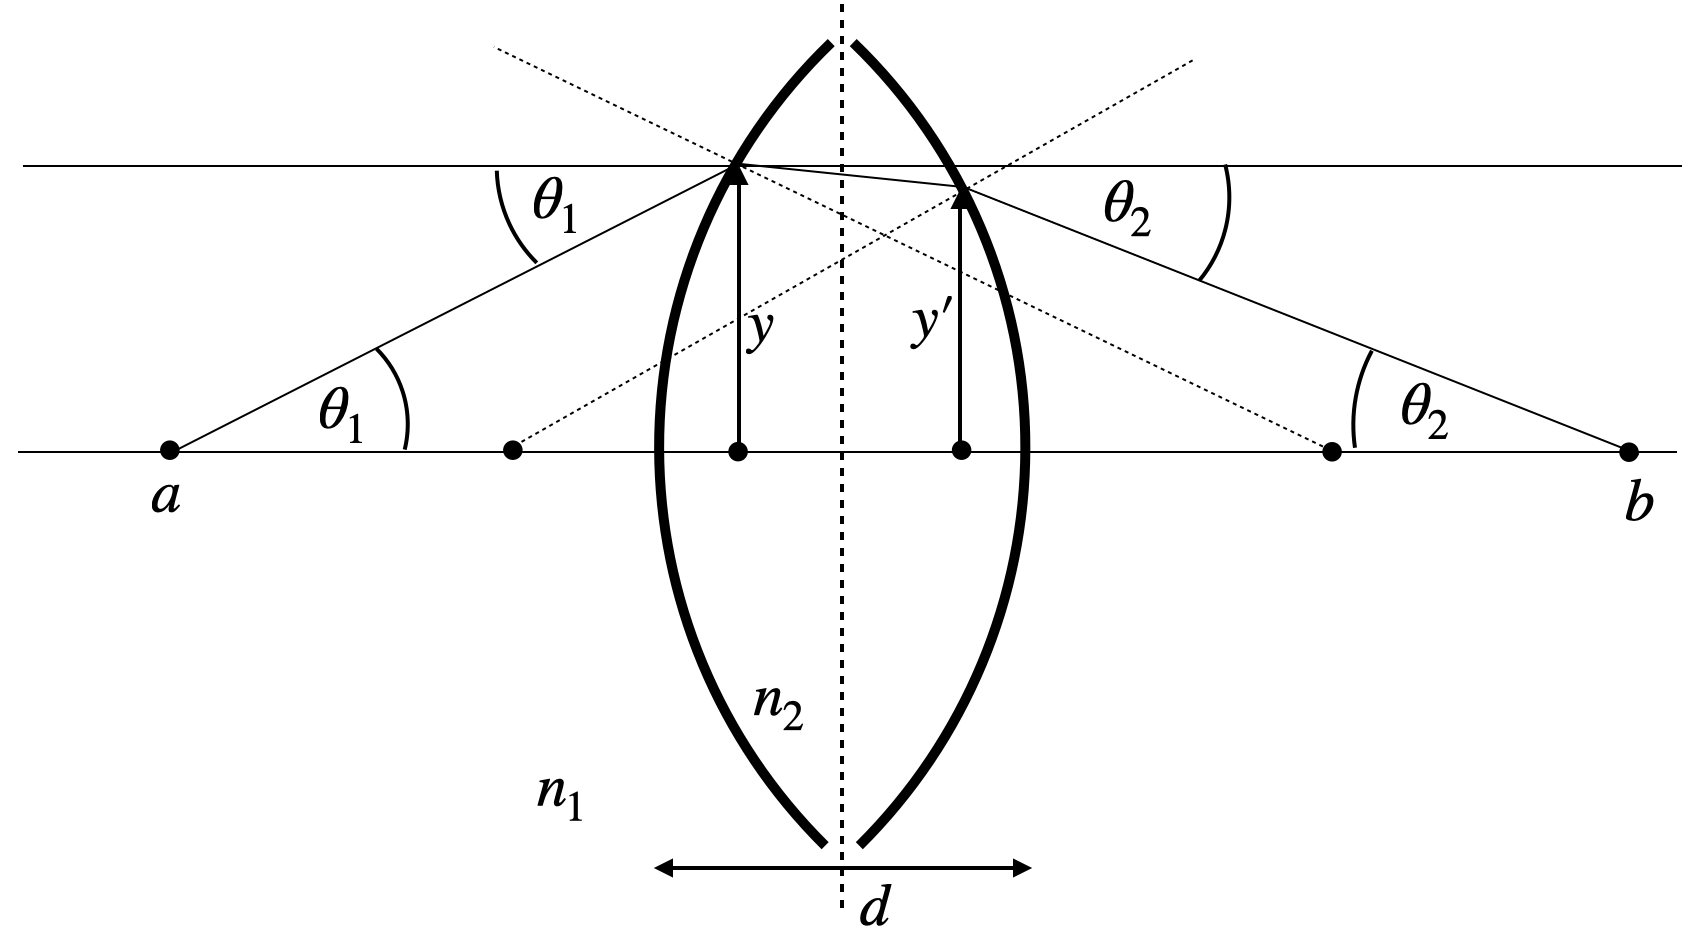
\includegraphics[width=0.6\linewidth,height=\textheight,keepaspectratio]{geometrical-optics/img/thin_lens.png}

}

\caption{\label{fig-thin-lens-refraction}Refraction on two spherical
surfaces.}

\end{figure}%

For thin lenses, where the thickness \(d\) is much smaller than \(R_1\)
and \(R_2\) (\(d \ll R_1, R_2\)), we can simplify our analysis. We
assume that the height of the ray at both surfaces is approximately
equal (\(y \approx y'\)), neglecting the displacement inside the lens.

This simplification allows us to treat all refraction as occurring on a
single plane at the lens center, known as the \textbf{principal plane}.
This concept, illustrated by the dashed line in the figure, greatly
simplifies optical calculations and ray tracing for thin lenses.

The radii's sign convention (positive for convex surfaces facing
incident light, negative for concave) and this two-surface analysis form
the basis for the thin lens formula. This formula relates object
distance, image distance, and focal length, encapsulating the lens's
imaging properties.

The result of the above calculation is leading to the imaging equation
for the thin lens.

\begin{tcolorbox}[enhanced jigsaw, breakable, toptitle=1mm, bottomrule=.15mm, colbacktitle=quarto-callout-note-color!10!white, title=\textcolor{quarto-callout-note-color}{\faInfo}\hspace{0.5em}{Imaging Equation for Thin Lens}, arc=.35mm, rightrule=.15mm, bottomtitle=1mm, opacityback=0, toprule=.15mm, coltitle=black, leftrule=.75mm, opacitybacktitle=0.6, colback=white, left=2mm, titlerule=0mm, colframe=quarto-callout-note-color-frame]

The sum of the inverse object and image distances equals the inverse
focal length of the thin lens:

\[\frac{1}{a}+\frac{1}{b}\approx\frac{n_2-n_1}{n_1}\left (\frac{1}{R_1}-\frac{1}{R_2}\right )=\frac{1}{f}\]

\end{tcolorbox}

\begin{tcolorbox}[enhanced jigsaw, breakable, toptitle=1mm, bottomrule=.15mm, colbacktitle=quarto-callout-note-color!10!white, title=\textcolor{quarto-callout-note-color}{\faInfo}\hspace{0.5em}{Lensmaker equation}, arc=.35mm, rightrule=.15mm, bottomtitle=1mm, opacityback=0, toprule=.15mm, coltitle=black, leftrule=.75mm, opacitybacktitle=0.6, colback=white, left=2mm, titlerule=0mm, colframe=quarto-callout-note-color-frame]

The focal length of a thin lens is calculated by the \textbf{lensmaker
equation}:
\[f=\frac{n_1}{n_2-n_1}\left ( \frac{R_1 R_2}{R_2 -R_1}\right)\]

in the paraxial approximation.

\end{tcolorbox}

The equation for the focal length has some important consequence. It
says that if the difference of the refractive indices inside (\(n_2\))
and outside \(n_1\) get smaller, the focal length becomes larger and
finally infinity. This can be nicely observed by placing a lens outside
and inside a water filled basin as shown below.

\begin{figure}

\begin{minipage}{0.50\linewidth}

\centering{

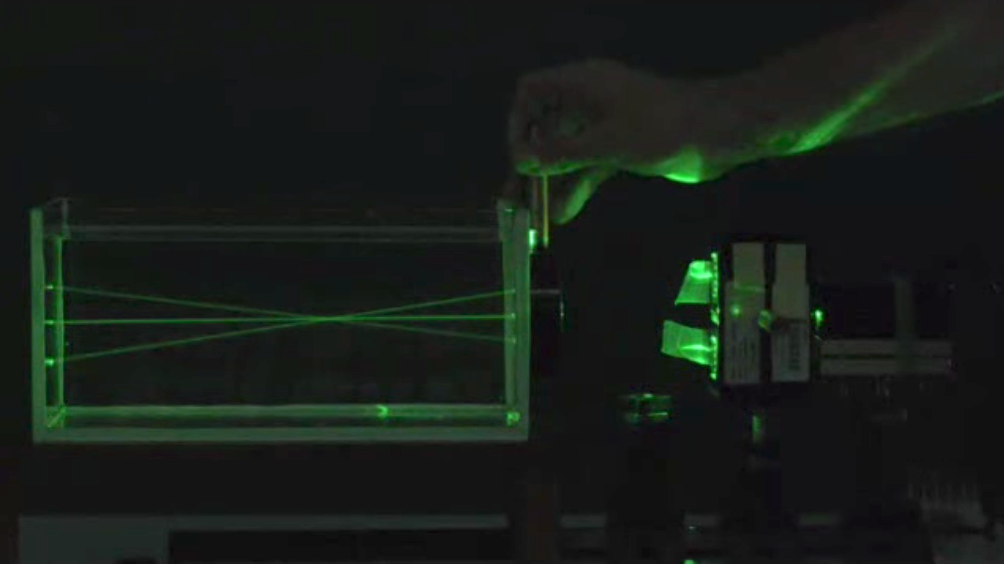
\includegraphics[width=1\linewidth,height=\textheight,keepaspectratio]{geometrical-optics/expimg/lens_contrast_out.png}

}

\subcaption{\label{fig-lens-air}Lens in air}

\end{minipage}%
%
\begin{minipage}{0.50\linewidth}

\centering{

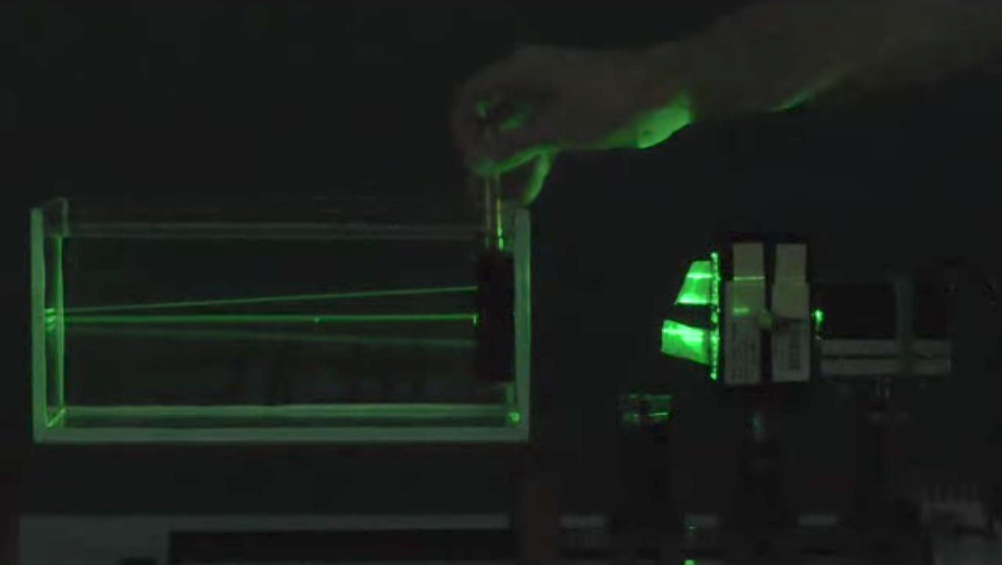
\includegraphics[width=1\linewidth,height=\textheight,keepaspectratio]{geometrical-optics/expimg/lens_contrast_in.png}

}

\subcaption{\label{fig-lens-water}Lens in water}

\end{minipage}%

\caption{\label{fig-lens-contrast}Focusing of parallel rays by a lens in
air (\(n_1=1\), left) and in water (\(n_1=1.36\), right). The images
clearly show the change in focal length between the two situations.}

\end{figure}%

\begin{tcolorbox}[enhanced jigsaw, breakable, toptitle=1mm, bottomrule=.15mm, colbacktitle=quarto-callout-note-color!10!white, title=\textcolor{quarto-callout-note-color}{\faInfo}\hspace{0.5em}{Bessel's method to measure the focal length of a lens}, arc=.35mm, rightrule=.15mm, bottomtitle=1mm, opacityback=0, toprule=.15mm, coltitle=black, leftrule=.75mm, opacitybacktitle=0.6, colback=white, left=2mm, titlerule=0mm, colframe=quarto-callout-note-color-frame]

The is an interesting way to measure the focal length of a lens. Fix a
distance \(D\) between object and screen. Then place a converging lens
between them. Due to the reversibility of the light path, the lens will
create a sharp image on the screen at two positions, which are separated
by a distance \(d\).

The equation for the focal distance can then be obtained from the

\begin{itemize}
\tightlist
\item
  Lens equation: \(\frac{1}{f} = \frac{1}{a} + \frac{1}{b}\)
\item
  Total distance: \(D = a + b\)
\end{itemize}

Where \(f\) is focal length, \(a\) is object distance, and \(b\) is
image distance. To obtain the focal distance according to this method,
which is called the \textbf{Bessel method}, the following steps are
taken:

For the first lens position:

\[D = a_1 + b_1\]

For the second lens position:

\[D = a_2 + b_2\]

We can further calculate the distance between the two lens positions:

\[d = a_1 - a_2 = b_2 - b_1\]

and use the imaging equation to find the focal length:

\[\frac{1}{f} = \frac{1}{a_1} + \frac{1}{b_1} = \frac{1}{a_2} + \frac{1}{b_2}\]

Substituting \(b_1 = D - a_1\) and \(b_2 = D - a_2\) we get further

\[\frac{1}{f} = \frac{1}{a_1} + \frac{1}{D-a_1} = \frac{1}{a_2} + \frac{1}{D-a_2}\]

Both euqations can be solved by

\[a_1 = \frac{D + d}{2} \quad \text{and} \quad a_2 = \frac{D - d}{2}\]

If we substitute that back into the imaging equation we obtain

\[\frac{1}{f} = \frac{2}{D} + \frac{2}{d}\]

which can be rearranged to get Bessel's formula:

\[f = \frac{D^2 - d^2}{4D}\]

This method only requires measuring \(D\) (fixed distance) and \(d\)
(distance between lens positions). It eliminates the need to know exact
object or image distances from the lens, making it more accurate than
methods requiring precise distance measurements from the lens.

\end{tcolorbox}

\subsubsection{Image Construction}\label{image-construction}

Images of objects can be now constructed if we refer to rays which do
not emerge from a position on the optical axis only. In this case, we
consider three different rays (two are actually enough). If we use as in
the case of a concave mirror a central and a parallel ray, we will find
a position where all rays cross on the other side. The conversion of the
rays is exactly the same as in the case of a spherical mirror. The
relation between the position of the object and the image along the
optical axis is described by the imaging equation.

\begin{figure}

\centering{

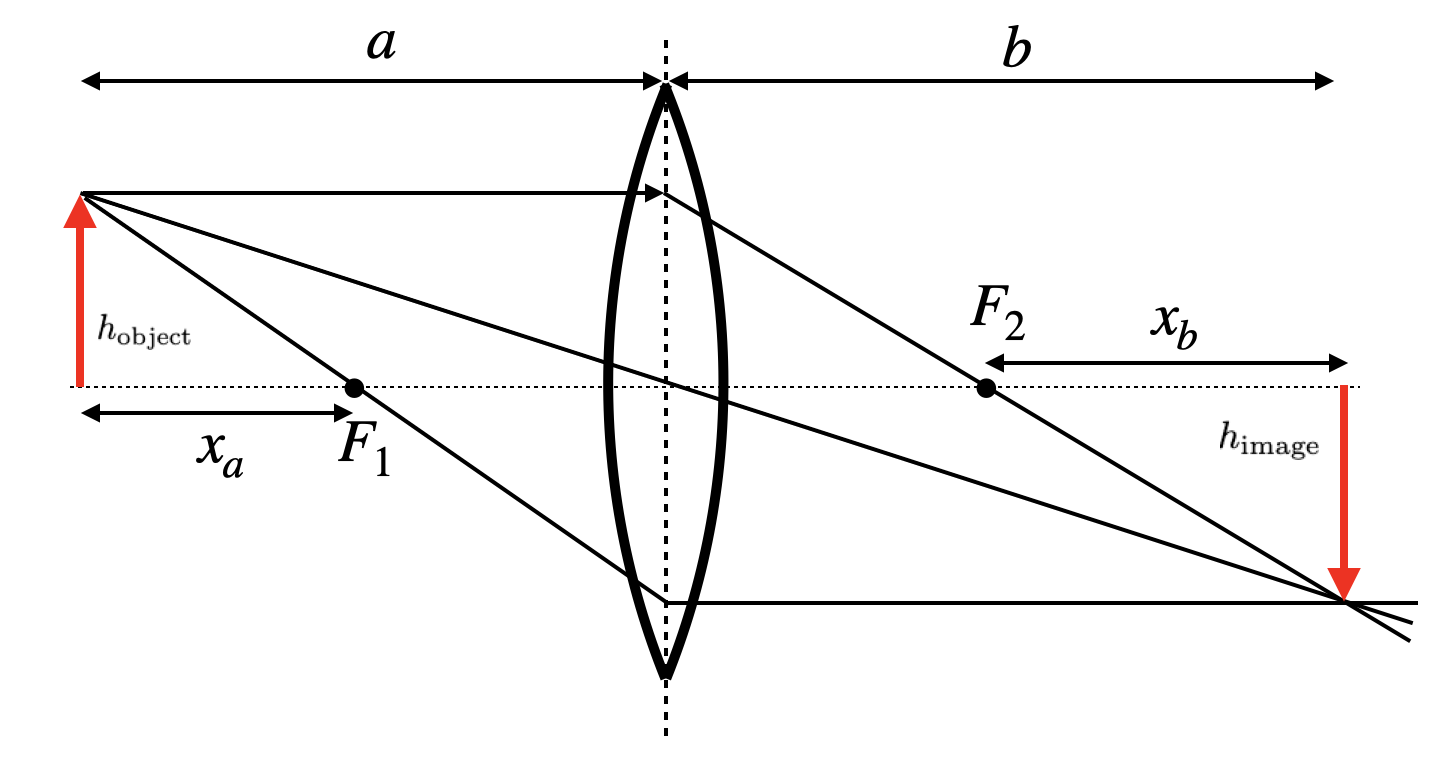
\includegraphics[width=0.6\linewidth,height=\textheight,keepaspectratio]{geometrical-optics/img/thin_lens_imaging.png}

}

\caption{\label{fig-thin-lens-imaging}Image construction on a thin
lens.}

\end{figure}%

Similar to the concave mirror, we may now also find out the image size
or the magnification of the lens.

\begin{tcolorbox}[enhanced jigsaw, breakable, toptitle=1mm, bottomrule=.15mm, colbacktitle=quarto-callout-note-color!10!white, title=\textcolor{quarto-callout-note-color}{\faInfo}\hspace{0.5em}{Magnification of a Lens}, arc=.35mm, rightrule=.15mm, bottomtitle=1mm, opacityback=0, toprule=.15mm, coltitle=black, leftrule=.75mm, opacitybacktitle=0.6, colback=white, left=2mm, titlerule=0mm, colframe=quarto-callout-note-color-frame]

The magnification is given by:

\[M=\frac{h_{\rm image}}{h_{\rm object}}=-\frac{b}{a}=\frac{f}{f-a}\]

where the negative sign is the result of the reverse orientation of the
real images created by a lens.

\end{tcolorbox}

According to our previous consideration \(M<0\) corresponds to a
reversed image, while it is upright as the object for \(M>0\). We,
therefore, easily see the following:

\begin{longtable}[]{@{}
  >{\raggedright\arraybackslash}p{(\linewidth - 6\tabcolsep) * \real{0.2361}}
  >{\raggedright\arraybackslash}p{(\linewidth - 6\tabcolsep) * \real{0.3333}}
  >{\raggedright\arraybackslash}p{(\linewidth - 6\tabcolsep) * \real{0.2639}}
  >{\raggedright\arraybackslash}p{(\linewidth - 6\tabcolsep) * \real{0.1667}}@{}}
\toprule\noalign{}
\begin{minipage}[b]{\linewidth}\raggedright
Object Position
\end{minipage} & \begin{minipage}[b]{\linewidth}\raggedright
Image Characteristics
\end{minipage} & \begin{minipage}[b]{\linewidth}\raggedright
Magnification (M)
\end{minipage} & \begin{minipage}[b]{\linewidth}\raggedright
Image Type
\end{minipage} \\
\midrule\noalign{}
\endhead
\bottomrule\noalign{}
\endlastfoot
\(a < f\) & Upright and magnified & \(M > 0\) & Virtual \\
\(f < a < 2f\) & Reversed and magnified & \(M < -1\) & Real \\
\(a = 2f\) & Reversed, same size & \(M = -1\) & Real \\
\(a > 2f\) & Reversed and shrunk & \(-1 < M < 0\) & Real \\
\(a = f\) & Appears at infinity & \(M = \infty\) & - \\
\end{longtable}

The image below illustrates the construction of images in 4 of the above
cases for a bi-convex lens, including the generation of a virtual image.

\begin{longtable}[]{@{}
  >{\raggedright\arraybackslash}p{(\linewidth - 0\tabcolsep) * \real{1.0000}}@{}}
\toprule\noalign{}
\begin{minipage}[b]{\linewidth}\raggedright
\end{minipage} \\
\midrule\noalign{}
\endhead
\bottomrule\noalign{}
\endlastfoot
\textbf{Fig.:} Image construction on a biconvex lens with a parallel and
a central ray for different object distances. \\
\end{longtable}

\subsection{Thick lens}\label{thick-lens}

For a thin lens, the displacement of the beam in height
(\(y,y^{\prime}\)) due to the thickness has been neglected. That means
that we can reduce all refracting action of the lens to a single plane,
which we call a principle plane. This approximation is (independent of
the paraxial approximation) not anymore true for lenses if the
displacement \(\Delta\) of the ray as in the image below cannot be
neglected. Such lenses are called \textbf{thick lenses} and they do not
have a single principle plane anymore. In fact, the principle plane
splits up into two principle planes at a distance \(h\).

\begin{figure}

\centering{

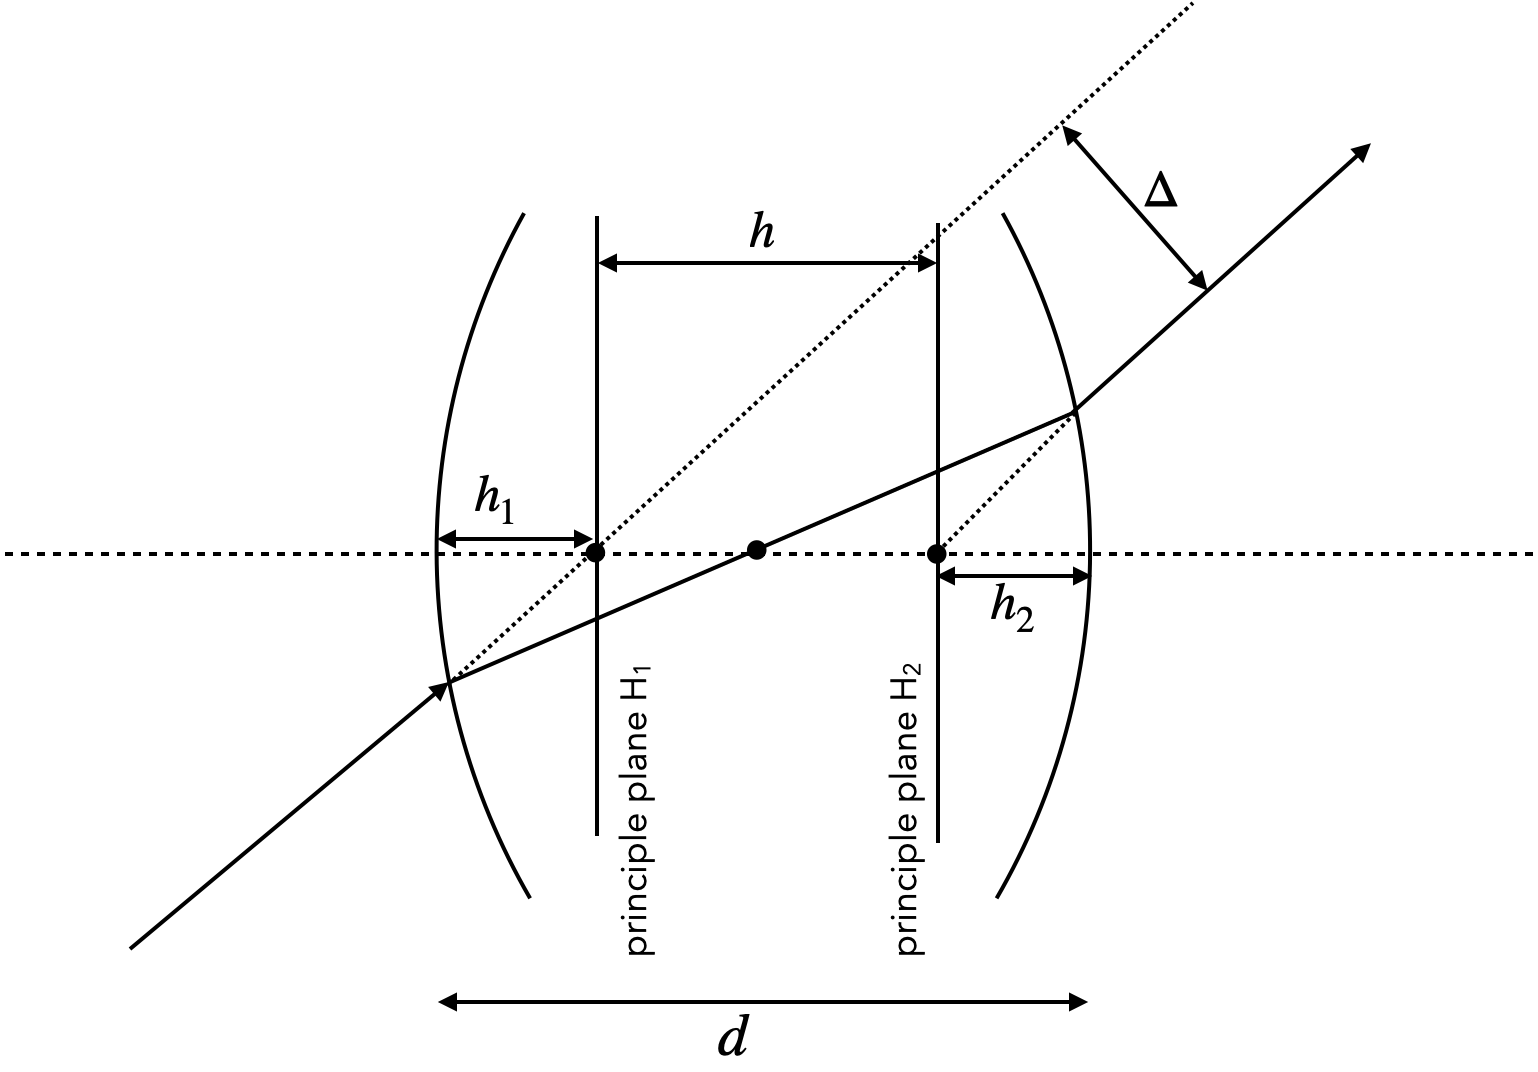
\includegraphics[width=0.8\linewidth,height=\textheight,keepaspectratio]{geometrical-optics/img/thick_lens.png}

}

\caption{\label{fig-thick-lens-planes}Thick lens principal planes.}

\end{figure}%

As indicated in the sketch above, an incident ray which is not deflected
can be extended to its intersection with the optical axis at a point,
which is a distance \(h_1\) behind the lens surface. This is the
location for the first principle plane. The position of the second
principle plane at a distance \(h_2\) before the back surface is found
for by reversing the ray path. According to that, both principle planes
have a distance \(h=d-h_1+h_2\) (mind the sign of the \(h\)). Using some
mathematical effort, one can show that the same imaging equation as for
a thins lens can be used with a new definition of the focal length and
taking into account that object and image distances refer to their
principle planes.

\newpage

\begin{tcolorbox}[enhanced jigsaw, breakable, toptitle=1mm, bottomrule=.15mm, colbacktitle=quarto-callout-note-color!10!white, title=\textcolor{quarto-callout-note-color}{\faInfo}\hspace{0.5em}{Matrix Optics}, arc=.35mm, rightrule=.15mm, bottomtitle=1mm, opacityback=0, toprule=.15mm, coltitle=black, leftrule=.75mm, opacitybacktitle=0.6, colback=white, left=2mm, titlerule=0mm, colframe=quarto-callout-note-color-frame]

The above derived equations for a single spherical surface yield a
linear relation between the input variables \(y_1\) and \(\theta_1\) and
the output variables \(y_2\) and \(\theta_2\). The linear relation
yields a great opportunity to express optical elements in terms of
linear transformations (matrices). This is the basis of \textbf{matrix
optics}. The matrix representation of a lens is given by

\[\begin{pmatrix} y_2 \\ \theta_2 \end{pmatrix} = \begin{pmatrix} 1 & 0 \\ -\frac{1}{f} & 1 \end{pmatrix} \begin{pmatrix} y_1 \\ \theta_1 \end{pmatrix}\]

where the matrix is called the \textbf{ABCD matrix} of the lens. Due to
the linearization of Snells law w can write down more generally

\[\begin{pmatrix} y_2 \\
\theta_2 \end{pmatrix} = \begin{pmatrix} A & B \\ C & D \end{pmatrix} \begin{pmatrix} y_1 \\ \theta_1 \end{pmatrix}\]

and one can obtain a Matrix for all types of optical elements such as
free space of dustance \(d\).

\[\begin{bmatrix}
A & B\\
C & D
\end{bmatrix}
=
\begin{bmatrix}
1 & d\\
0 & 1
\end{bmatrix}
\]

The physical meaning of the ABCD matrix elements can be understood as
follows:

\begin{longtable}[]{@{}
  >{\raggedright\arraybackslash}p{(\linewidth - 2\tabcolsep) * \real{0.3462}}
  >{\raggedright\arraybackslash}p{(\linewidth - 2\tabcolsep) * \real{0.6538}}@{}}
\toprule\noalign{}
\begin{minipage}[b]{\linewidth}\raggedright
Element
\end{minipage} & \begin{minipage}[b]{\linewidth}\raggedright
Physical Meaning
\end{minipage} \\
\midrule\noalign{}
\endhead
\bottomrule\noalign{}
\endlastfoot
\textbf{A} & Relates output height to input height (magnification-like
effect) \\
\textbf{B} & Relates output height to input angle (how much an angled
ray displaces) \\
\textbf{C} & Relates output angle to input height (optical power,
focusing/defocusing) \\
\textbf{D} & Relates output angle to input angle (angular
magnification) \\
\end{longtable}

Here are some useful matrices for optical elements:

\[
\mathbf{M}=\left[\begin{array}{ll}
1 & d \\
0 & 1
\end{array}\right] \tag{Free space}
\]

\[
\mathbf{M}=\left[\begin{array}{cc}
1 & 0 \\
0 & \frac{n_1}{n_2}
\end{array}\right] \tag{Planar interface}
\]

\[
\mathbf{M}=\left[\begin{array}{cc}
1 & 0 \\
-\frac{\left(n_2-n_1\right)}{n_2 R} & \frac{n_1}{n_2}
\end{array}\right] \tag{Spherical Boundary}
\]

\[
\mathbf{M}=\left[\begin{array}{cc}
1 & 0 \\
-\frac{1}{f} & 1
\end{array}\right] \tag{Tin Lens}
\]

If we have now a system of optical elements, we can multiply the
matrices of the individual elements to obtain the matrix of the whole
system.

\[
\rightarrow \mathrm{M}_1 \rightarrow \mathrm{M}_2 \rightarrow \mathrm{M}_N \rightarrow \mathrm{M}=\mathbf{M}_N \ldots \mathrm{M}_2 \mathbf{M}_1 \text {. }
\]

This is a very powerful tool to analyze optical systems.

\subsection{Example: Two-Lens System}\label{example-two-lens-system}

Consider a system consisting of two thin lenses separated by a distance
\(d\). The first lens has focal length \(f_1 = 100\) mm and the second
lens has focal length \(f_2 = 150\) mm, separated by \(d = 200\) mm. We
want to find the overall system matrix and determine where a parallel
ray at height \(y_1 = 10\) mm crosses the optical axis.

The system consists of three components: 1. First lens with matrix
\(\mathbf{M}_1\) 2. Free space propagation of distance \(d\) with matrix
\(\mathbf{M}_{\text{free}}\) 3. Second lens with matrix \(\mathbf{M}_2\)

The individual matrices are:

\[
\mathbf{M}_1 = \begin{bmatrix} 1 & 0 \\ -\frac{1}{f_1} & 1 \end{bmatrix}, \quad
\mathbf{M}_{\text{free}} = \begin{bmatrix} 1 & d \\ 0 & 1 \end{bmatrix}, \quad
\mathbf{M}_2 = \begin{bmatrix} 1 & 0 \\ -\frac{1}{f_2} & 1 \end{bmatrix}
\]

The total system matrix is:

\[
\mathbf{M}_{\text{total}} = \mathbf{M}_2 \cdot \mathbf{M}_{\text{free}} \cdot \mathbf{M}_1
\]

Performing the matrix multiplication:

\[
\mathbf{M}_{\text{total}} = \begin{bmatrix} 1 & 0 \\ -\frac{1}{f_2} & 1 \end{bmatrix} \begin{bmatrix} 1 & d \\ 0 & 1 \end{bmatrix} \begin{bmatrix} 1 & 0 \\ -\frac{1}{f_1} & 1 \end{bmatrix}
\]

\[
= \begin{bmatrix} 1 & 0 \\ -\frac{1}{f_2} & 1 \end{bmatrix} \begin{bmatrix} 1 - \frac{d}{f_1} & d \\ -\frac{1}{f_1} & 1 \end{bmatrix}
\]

\[
= \begin{bmatrix} 1 - \frac{d}{f_1} & d \\ -\frac{1}{f_2} - \frac{1}{f_1} + \frac{d}{f_1 f_2} & 1 - \frac{d}{f_2} \end{bmatrix}
\]

For our specific values (\(f_1 = 100\) mm, \(f_2 = 150\) mm, \(d = 200\)
mm):

\[
\mathbf{M}_{\text{total}} = \begin{bmatrix} -1 & 200 \\ -0.00333 & -0.333 \end{bmatrix}
\]

For a parallel ray at height \(y_1 = 10\) mm (i.e., \(\theta_1 = 0\)):

\[
\begin{pmatrix} y_2 \\ \theta_2 \end{pmatrix} = \begin{bmatrix} -1 & 200 \\ -0.00333 & -0.333 \end{bmatrix} \begin{pmatrix} 10 \\ 0 \end{pmatrix} = \begin{pmatrix} -10 \\ -0.0333 \end{pmatrix}
\]

The ray exits at height \(y_2 = -10\) mm with angle
\(\theta_2 = -0.0333\) rad. The ray crosses the optical axis at a
distance:

\[
b = -\frac{y_2}{\theta_2} = -\frac{-10}{-0.0333} = -300 \text{ mm}
\]

This means the focal point is 300 mm before the second lens (a virtual
focus). This example demonstrates how matrix optics simplifies the
analysis of complex multi-element optical systems.

\end{tcolorbox}

\begin{tcolorbox}[enhanced jigsaw, breakable, toptitle=1mm, bottomrule=.15mm, colbacktitle=quarto-callout-note-color!10!white, title=\textcolor{quarto-callout-note-color}{\faInfo}\hspace{0.5em}{Thick Lens Focal Length}, arc=.35mm, rightrule=.15mm, bottomtitle=1mm, opacityback=0, toprule=.15mm, coltitle=black, leftrule=.75mm, opacitybacktitle=0.6, colback=white, left=2mm, titlerule=0mm, colframe=quarto-callout-note-color-frame]

We would like to model the imaging properties of a thick lens using the
matrix method. The lens is divided into three components:

\begin{enumerate}
\def\labelenumi{\arabic{enumi}.}
\tightlist
\item
  A spherical surface at the front of the lens with radius \(R_1\)
\item
  A region of free space propagation through the lens material of
  thickness \(d\)
\item
  Another spherical surface at the back of the lens with radius \(R_2\)
\end{enumerate}

The matrices for these components are:

\[
M_1 = \begin{bmatrix} 1 & 0 \\ -1/f_1 & 1/n \end{bmatrix}, \quad
M_2 = \begin{bmatrix} 1 & d \\ 0 & 1 \end{bmatrix}, \quad
M_3 = \begin{bmatrix} 1 & 0 \\ -1/f_2 & n \end{bmatrix}
\]

Where - \(f_1\) and \(f_2\) are the focal lengths of the front and back
surfaces, which are determined by the radii of curvature \(R_1\) and
\(R_2\) of the surfaces - \(d\) is the thickness of the lens, measured
along the optical axis

\section{Derivation}\label{derivation}

For a lens with refractive index \(n\) in air, the focal lengths of the
surfaces are:

\[\frac{1}{f_1} = \frac{1-n}{nR_1}, \quad \frac{1}{f_2} = \frac{n-1}{R_2}\]

Where \(R_1\) and \(R_2\) are the radii of curvature of the front and
back surfaces.

The total system matrix is then

\[M_{total} = M_3 \cdot M_2 \cdot M_1\]

After multiplication the total matrix is

\[
M=\begin{bmatrix}
  1 - \frac{d \left(1 - n\right)}{R_{1}} & d\\
  - \frac{n-1}{R_{2} } - \frac{\left(1 - n\right) \left(n - \frac{d n \left( n-1\right)}{R_{2}}\right)}{R_{1} n} & \frac{\left(n - \frac{d n \left( n-1\right)}{R_{2}}\right)}{n}
\end{bmatrix}
\]

where the element in the lower left corner is the inverse of the focal
length of the thick lens. This can be simplified to the following
expression:

\[-\frac{1}{f} = -\frac{1}{f_2} - \frac{n}{f_1} -\frac{d n}{f_1f_2}\]

Substituting the expressions for \(1/f_1\) and \(1/f_2\):

\[\frac{1}{f} = \frac{n-1}{R_1} - \frac{n-1}{R_2} + \frac{d(n-1)^2}{nR_1R_2}\]

Factoring out \((n-1)\) gives the final expression for the focal length
of a thick lens:

\[\frac{1}{f} = (n-1)\left[\frac{1}{R_1} - \frac{1}{R_2} + \frac{(n-1)d}{R_1R_2}\right]\]

This is the Lensmaker's equation for a thick lens.

The construction of ray diagrams for thick lenses is similar to that for
thin lenses, but the object and image distances are measured from the
principal planes. The magnification is also calculated using the
distances from the principal planes. \textbf{Principal planes are where
a thick lens can be treated as an equivalent thin lens. At these planes,
the magnification is unity.}

The derivation of the local of the principle planes will be part of the
seminar.

\begin{verbatim}
\end{verbatim}

$\displaystyle 1/f =\frac{n_{1} - n_{2}}{R_{2} n_{1}} - \frac{n_{1} - n_{2}}{R_{1} n_{1}} + \frac{d \left(n_{1} - n_{2}\right)^{2}}{R_{1} R_{2} n_{1}}$

\end{tcolorbox}

\begin{tcolorbox}[enhanced jigsaw, breakable, toptitle=1mm, bottomrule=.15mm, colbacktitle=quarto-callout-note-color!10!white, title=\textcolor{quarto-callout-note-color}{\faInfo}\hspace{0.5em}{Imaging Equation for Thick Lens}, arc=.35mm, rightrule=.15mm, bottomtitle=1mm, opacityback=0, toprule=.15mm, coltitle=black, leftrule=.75mm, opacitybacktitle=0.6, colback=white, left=2mm, titlerule=0mm, colframe=quarto-callout-note-color-frame]

The sum of the inverse object and image distances to the principal
planes (\(H_1,H_2\)) equals the inverse focal length of the thick lens:

\[\frac{1}{a}+\frac{1}{b}\approx\frac{1}{f}, \quad \text{where} \quad \frac{1}{f}=n-1\left (\frac{1}{R_1}-\frac{1}{R_2}+\frac{(n-1)d}{n R_1 R_2}\right )\]

in the paraxial approximation. The construction of the image on a thick
lens is done with the help of two principle planes. The object distance
\(a\) and the image distance \(b\) are measured from these principle
planes. The location of the two principle planes are found to be

\[h_{1}=-\frac{(n-1)f d}{n R_2}\]

\[h_{2}=-\frac{(n-1)f d}{n R_1}\]

\end{tcolorbox}

As compared to the construction of an image on a thin lens, we now have
to consider some pecularities for the thick lens. An incident parallel
ray, which turns into a focal ray is now refracted at the second
principle plane. The reverse must, therefore, be true for an incident
focal ray. This ray is refracted on the first principle plane. The
central ray is deflected on both principle planes. It is incident under
a certain angle at the first principle plane and outgoing with the same
principle angle to the second principle plane. The sketch below
summarizes these issues for a thick lens.

\begin{figure}

\centering{

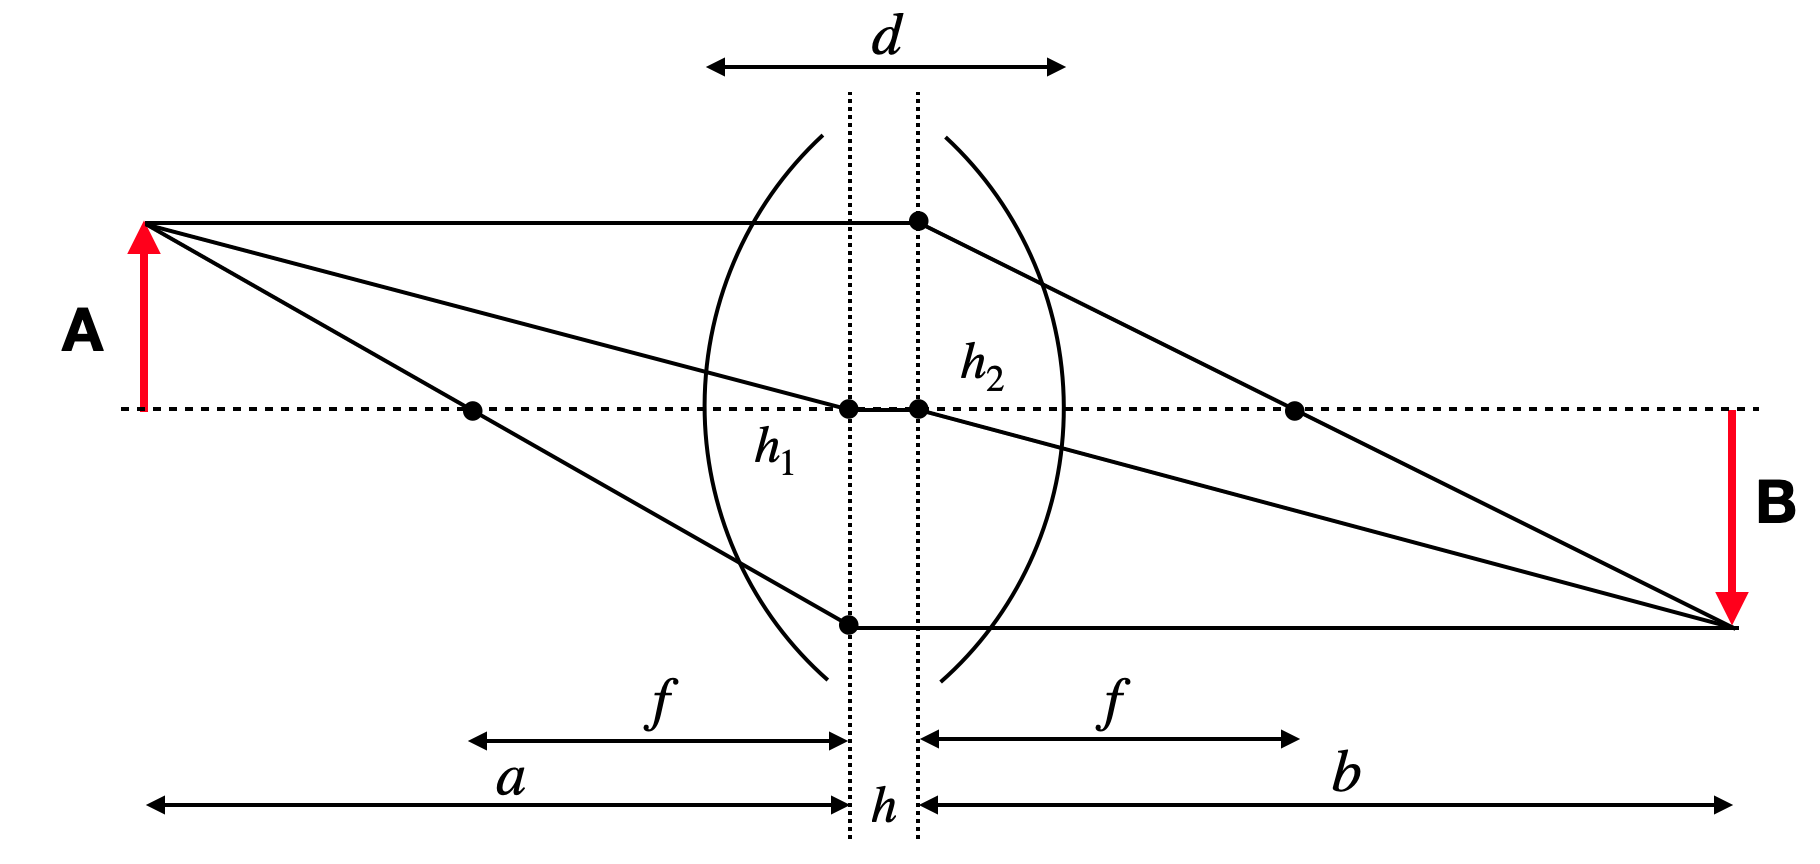
\includegraphics[width=0.7\linewidth,height=\textheight,keepaspectratio]{geometrical-optics/img/thick_lens_construction.png}

}

\caption{\label{fig-thick-lens}Thick lens image construction.}

\end{figure}%

\subsection{Lens types}\label{lens-types}

Depending on the radii of curvature and their sign, one can construct
different types of lenses that are used in many applications. Modern
microscopy lenses, for example, can contain up to 20 different lenses,
each with carefully designed curvatures and materials to correct for
various optical aberrations and achieve high-quality imaging.

\begin{figure}

\centering{

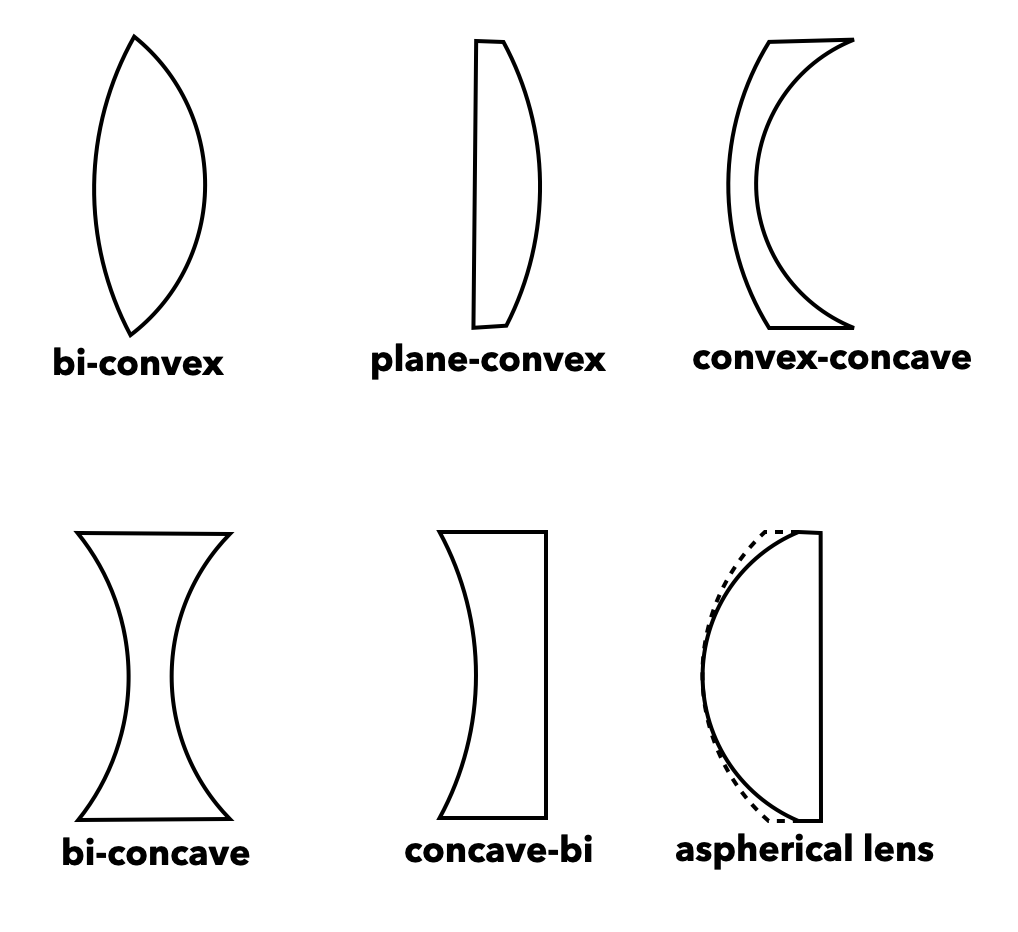
\includegraphics[width=0.4\linewidth,height=\textheight,keepaspectratio]{geometrical-optics/img/lens_types.png}

}

\caption{\label{fig-lens-types}Different lens types.}

\end{figure}%

\begin{figure}

\begin{minipage}{0.33\linewidth}

\centering{

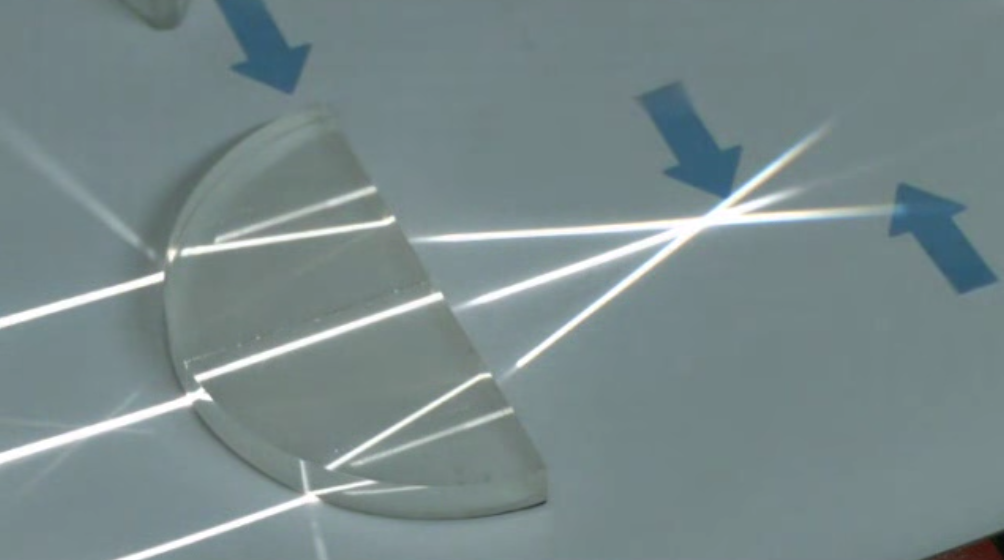
\includegraphics[width=1\linewidth,height=\textheight,keepaspectratio]{geometrical-optics/expimg/convex_plane_thick.png}

}

\subcaption{\label{fig-convex-thick}Convex plane thick}

\end{minipage}%
%
\begin{minipage}{0.33\linewidth}

\centering{

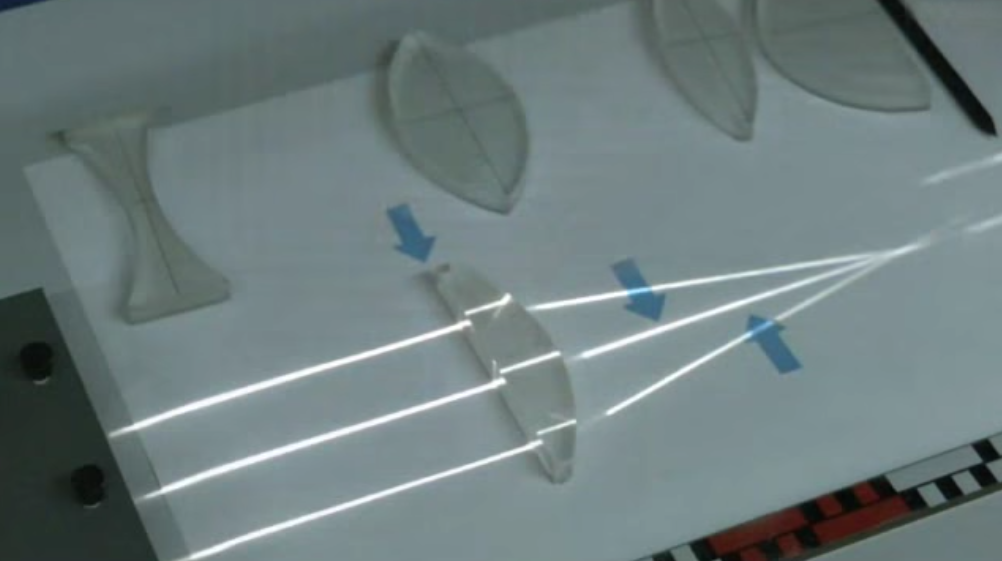
\includegraphics[width=1\linewidth,height=\textheight,keepaspectratio]{geometrical-optics/expimg/convex_plane_thin.png}

}

\subcaption{\label{fig-convex-thin}Convex plane thin}

\end{minipage}%
%
\begin{minipage}{0.33\linewidth}

\centering{

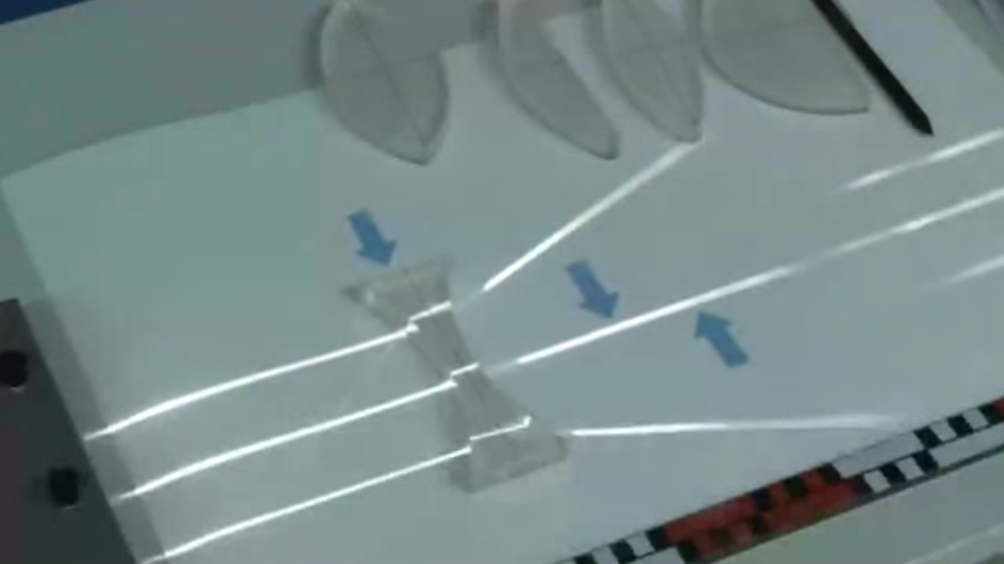
\includegraphics[width=1\linewidth,height=\textheight,keepaspectratio]{geometrical-optics/expimg/bi-concave_lens.png}

}

\subcaption{\label{fig-biconcave}Bi-concave lens}

\end{minipage}%

\caption{\label{fig-lens-focusing}Focusing behavior of a few different
lens types.}

\end{figure}%

\chapter{Optical Instruments}\label{optical-instruments}

\section{The Human Eye}\label{the-human-eye}

The human eye stands is one of the most remarkable sensory systems. This
sophisticated organ combines an array of precisely crafted
components---including an adjustable aperture, an adaptive lens, and a
highly sensitive photodetector---all interconnected with a neural
network capable of rapid and accurate pattern recognition. What's truly
astounding is that this entire system operates on mere watts of power.

\begin{figure}

\begin{minipage}{0.50\linewidth}

\centering{

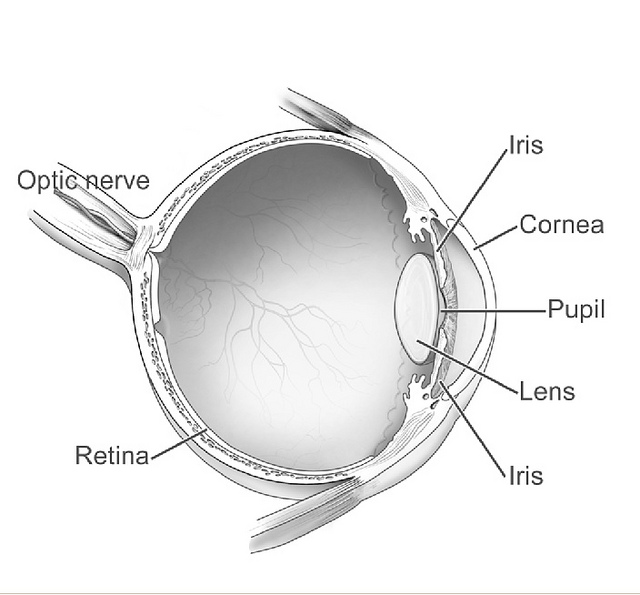
\includegraphics[width=1\linewidth,height=\textheight,keepaspectratio]{geometrical-optics/img/eye.jpeg}

}

\subcaption{\label{fig-eye-sketch}Anatomy of the human eye}

\end{minipage}%
%
\begin{minipage}{0.50\linewidth}

\centering{

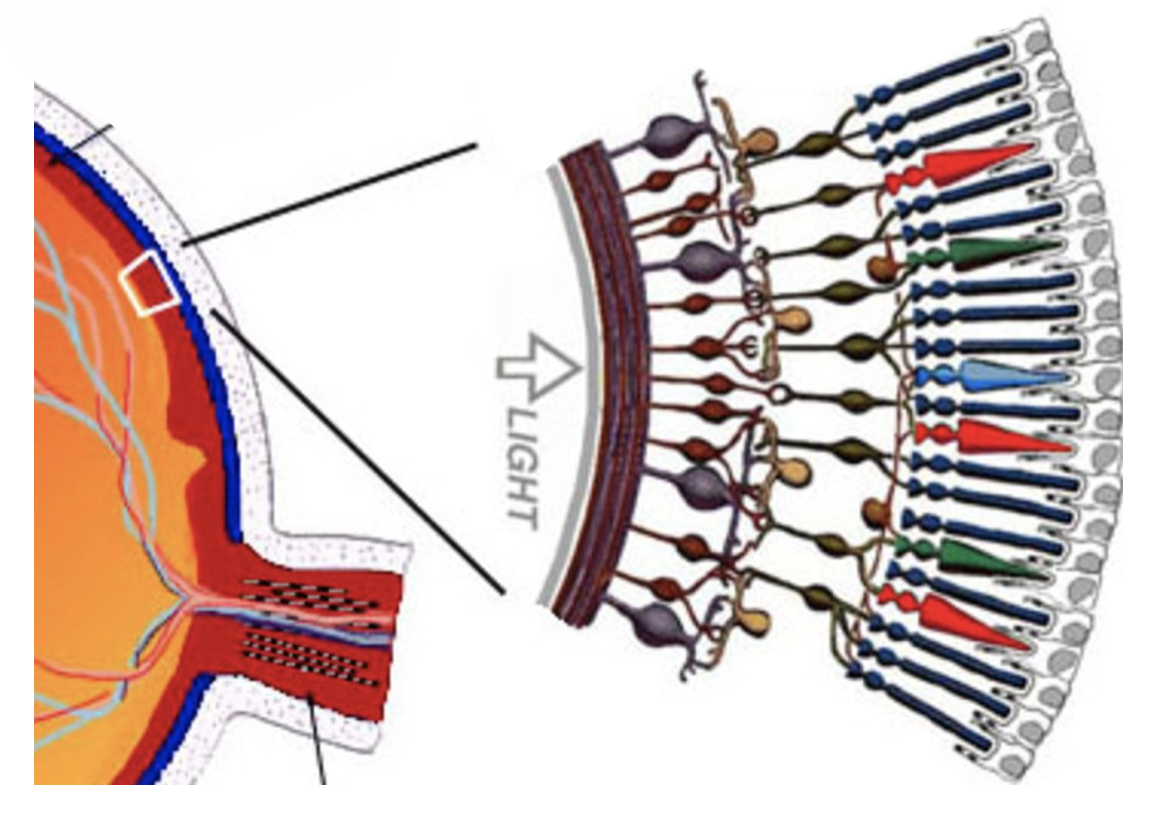
\includegraphics[width=1\linewidth,height=\textheight,keepaspectratio]{geometrical-optics/img/retina.png}

}

\subcaption{\label{fig-retina-detail}Retinal structure detail}

\end{minipage}%

\caption{\label{fig-eye}Left: Key components of the human eye, including
the lens, vitreous body, and retina with its light-sensitive cells.
Right: Detailed view of the retina, showing the arrangement and neural
connections of rods and cones.}

\end{figure}%

\subsection{Key Components and Their
Functions}\label{key-components-and-their-functions}

\begin{enumerate}
\def\labelenumi{\arabic{enumi}.}
\item
  \textbf{Pupil and Iris}: The pupil, surrounded by the iris, acts as an
  adjustable aperture. It regulates the amount of light entering the eye
  and influences the depth of field. In bright conditions, a constricted
  pupil increases the depth of field, allowing a wider range of
  distances to be in focus simultaneously.
\item
  \textbf{Lens}: Connected to the ciliary muscles, the lens can change
  its curvature to adjust focal length, a process known as
  accommodation. This allows the eye to focus on objects at varying
  distances.
\item
  \textbf{Vitreous Humor}: This gel-like substance fills the eye cavity,
  maintaining its shape and contributing to the eye's optical
  properties.
\item
  \textbf{Retina}: The light-sensitive layer at the back of the eye,
  containing photoreceptor cells (rods and cones) that convert light
  into neural signals.
\end{enumerate}

\subsection{Photoreceptors: Cones and
Rods}\label{photoreceptors-cones-and-rods}

The retina contains two types of photoreceptor cells:

\begin{enumerate}
\def\labelenumi{\arabic{enumi}.}
\item
  \textbf{Cones}: Responsible for color vision and high acuity in bright
  light. They are concentrated around the fovea, the area of highest
  visual acuity. There are about 6 Million cones in the human eye.
\item
  \textbf{Rods}: More sensitive to light but do not distinguish colors,
  providing vision in low light conditions. There are around 12 Million
  rods in the human eye.
\end{enumerate}

Rods and cones obtain their function from a chromophore molecule called
\textbf{retina}, which undergoes a conformational change when exposed to
light. This change triggers a cascade of chemical reactions that
ultimately lead to the generation of neural signals. The color vision is
achieved with the same chromophore molecule that is embedded in slightly
different protein structures in cones. This allows cones to be sensitive
to different wavelengths of light.

\begin{figure}

\centering{

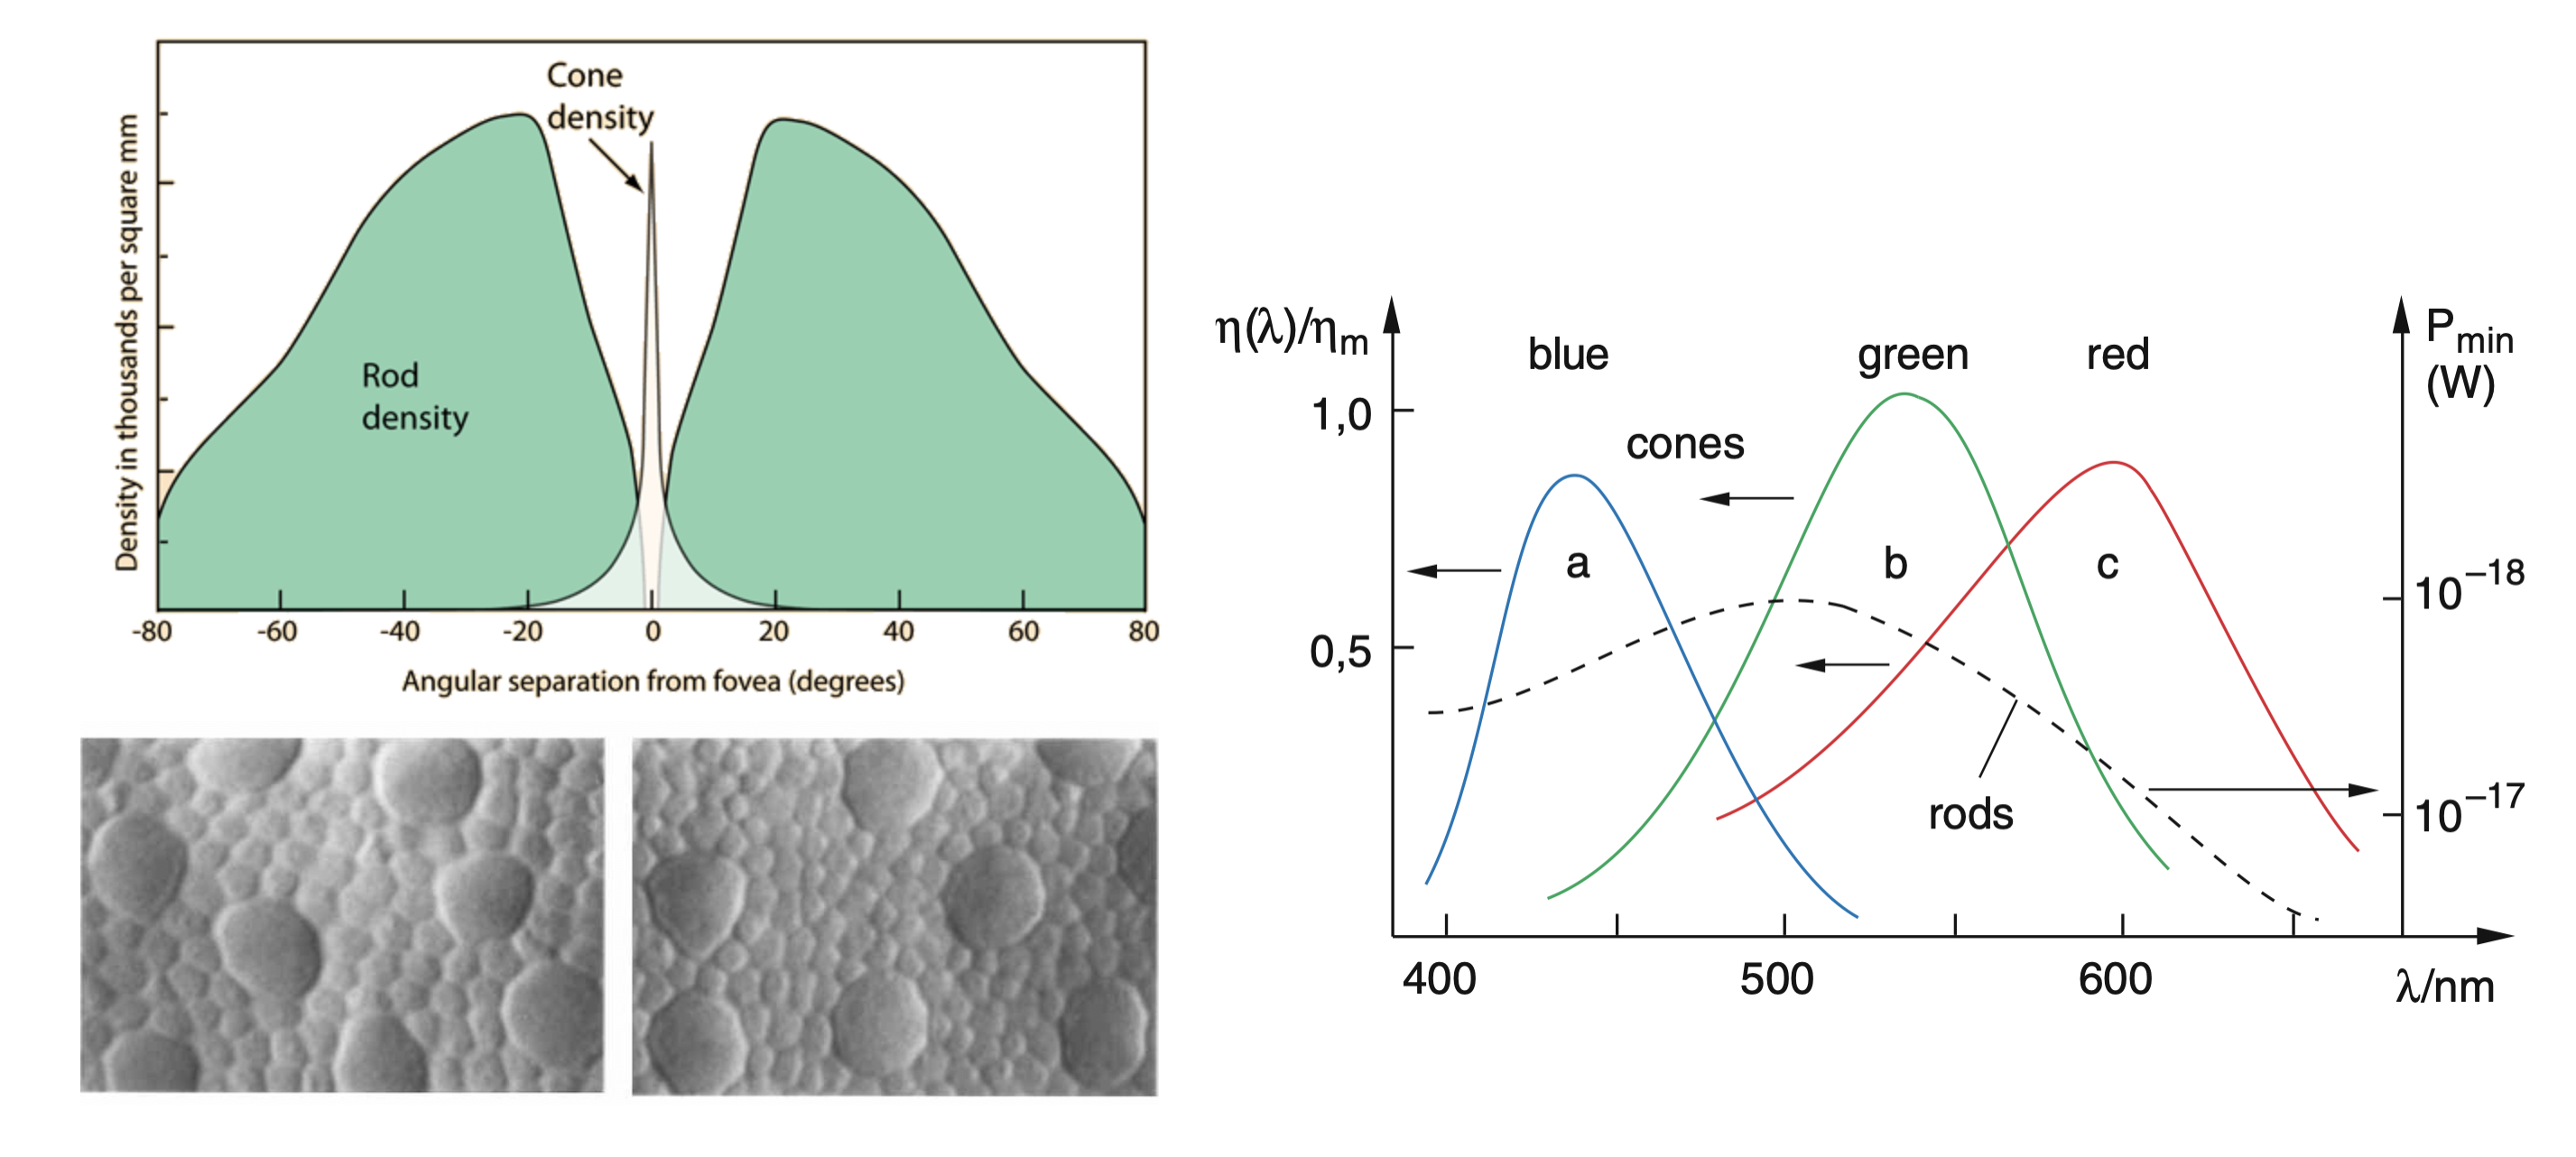
\includegraphics[width=0.9\linewidth,height=\textheight,keepaspectratio]{geometrical-optics/img/cone_and_rods.png}

}

\caption{\label{fig-cone-and-rods}Distribution of cones and rods around
the fovea, their microscopic structure, and spectral sensitivity.}

\end{figure}%

Cones contain light-sensitive pigments based on retinal molecules, which
undergo conformational changes when excited by light, triggering a
cascade of chemical processes. There are three types of cones, each
sensitive to different wavelengths of light, enabling color vision.

\subsection{Visual Acuity and
Performance}\label{visual-acuity-and-performance}

Visual acuity, often measured using an eye chart, quantifies the eye's
ability to resolve fine details. It's typically expressed as a fraction
(e.g., 20/20 vision), where the numerator is the test distance and the
denominator is the distance at which a person with normal acuity can
read the same line.

The human eye's remarkable performance in pattern recognition, depth
perception, and adaptability to varying light conditions is achieved
through the complex interplay of its optical components and neural
processing. This sophisticated system continues to inspire developments
in artificial vision systems and optical technologies.

\subsection{Optical Properties of the
Eye}\label{optical-properties-of-the-eye}

The eye's optical system is asymmetrical due to the different media it
interfaces with (air on one side, vitreous humor on the other). This
results in different focal lengths:

\begin{itemize}
\tightlist
\item
  Front focal length: \(f_1 = 17\) mm
\item
  Back focal length: \(f_2 = 22\) mm
\end{itemize}

These values can change during accommodation for near vision:

\begin{itemize}
\tightlist
\item
  Close object front focal length: \(f_1 = 14\) mm
\item
  Close object back focal length: \(f_2 = 19\) mm
\end{itemize}

The eye's refractive power, measured in diopters (D), is the reciprocal
of the focal length in meters. For a relaxed eye:

\[P = \frac{1}{f} = \frac{1}{0.022 \text{ m}} \approx 45.45 \text{ D}\]

During accommodation, this can increase to about 52 D.

\begin{figure}

\centering{

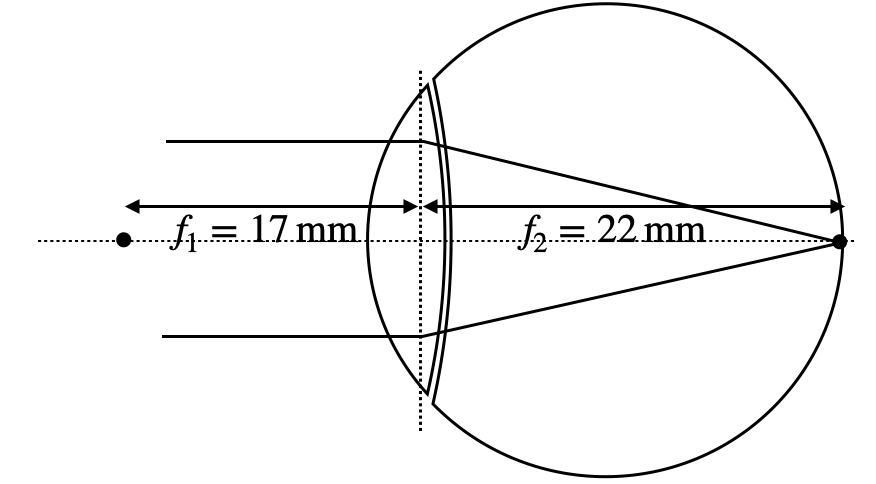
\includegraphics[width=0.4\linewidth,height=\textheight,keepaspectratio]{geometrical-optics/img/eye_focal_distance.png}

}

\caption{\label{fig-eye-focal-distance}Illustration of the eye's focal
distances.}

\end{figure}%

\subsection{Resolution Limit of the
Eye}\label{resolution-limit-of-the-eye}

The resolution of the eye is limited by diffraction and the spacing of
photoreceptors. The minimum angle of resolution θ\_min can be
approximated by:

\[\theta_{\text{min}} \approx \frac{1.22\lambda}{D}\]

where λ is the wavelength of light and D is the diameter of the pupil.
For a 3 mm pupil and 555 nm light (peak sensitivity), this gives a
theoretical resolution of about 1 arc minute.

\subsection{Refractive Errors and Visual
Correction}\label{refractive-errors-and-visual-correction}

The human eye, under normal conditions, focuses images of distant
objects onto the retina at the back focal distance of approximately 22
mm. However, various refractive errors can occur due to imperfections in
the eye's optical system, primarily the cornea and lens. These errors
affect the eye's ability to focus light accurately on the retina,
leading to vision problems.

Common refractive errors include:

\begin{enumerate}
\def\labelenumi{\arabic{enumi}.}
\item
  \textbf{Myopia (Short-sightedness)}: Light from distant objects
  focuses in front of the retina, causing distant objects to appear
  blurry while near objects remain clear.
\item
  \textbf{Hyperopia (Far-sightedness)}: Light focuses behind the retina,
  making nearby objects appear blurry while distant objects may remain
  clear.
\item
  \textbf{Astigmatism}: The cornea or lens isn't perfectly spherical,
  causing light to focus at multiple points rather than a single sharp
  point on the retina.
\end{enumerate}

\begin{figure}

\begin{minipage}{0.50\linewidth}

\centering{

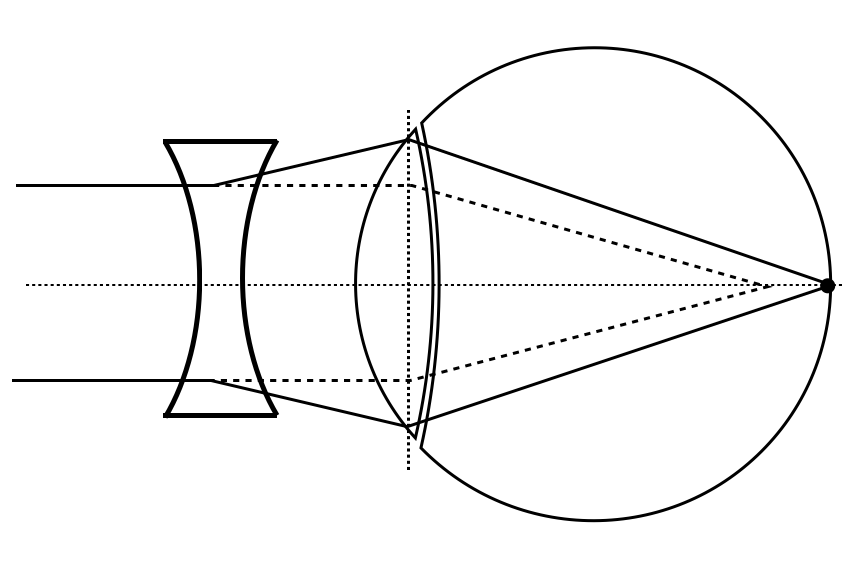
\includegraphics[width=1\linewidth,height=\textheight,keepaspectratio]{geometrical-optics/img/short_sighted.png}

}

\subcaption{\label{fig-short-sighted}Correction of Myopia}

\end{minipage}%
%
\begin{minipage}{0.50\linewidth}

\centering{

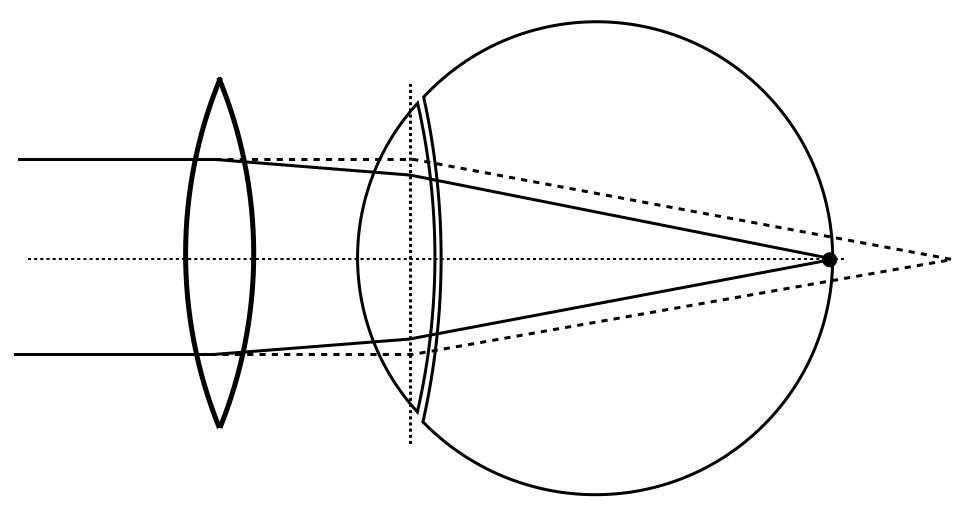
\includegraphics[width=1\linewidth,height=\textheight,keepaspectratio]{geometrical-optics/img/far_sighted.png}

}

\subcaption{\label{fig-far-sighted}Correction of Hyperopia}

\end{minipage}%

\caption{\label{fig-sight-correction}Left: Myopia correction using a
concave lens. Right: Hyperopia correction using a convex lens.}

\end{figure}%

The severity of refractive errors can be quantified using the concept of
refractive power. The refractive error R of the eye, measured in
diopters (D), is calculated as:

\[R = \frac{1}{f_{\text{required}}} - \frac{1}{f_{\text{actual}}}\]

where f\_required is the focal length needed for perfect focus, and
f\_actual is the eye's actual focal length. This formula helps determine
the degree of correction needed for various eye defects.

In a normal, relaxed state, the human eye can observe objects clearly up
to a distance of approximately \(s_0=25\) cm without additional
accommodation of the lens. This distance, known as the \textbf{range of
clear visual sight}, varies among individuals and is used as a standard
in optical calculations. Objects within this range can be observed under
a visual angle \(\epsilon_0\). For small angles, which is typically the
case in vision, the angular size \(\epsilon_0\) of an object of height h
at a distance \(s_0\) is approximated by:

\[
\epsilon_0 \approx \tan(\epsilon_0) = \frac{h}{s_0}
\]

This relationship is fundamental in understanding how objects are
perceived and in designing corrective lenses and optical instruments.

\begin{figure}

\centering{

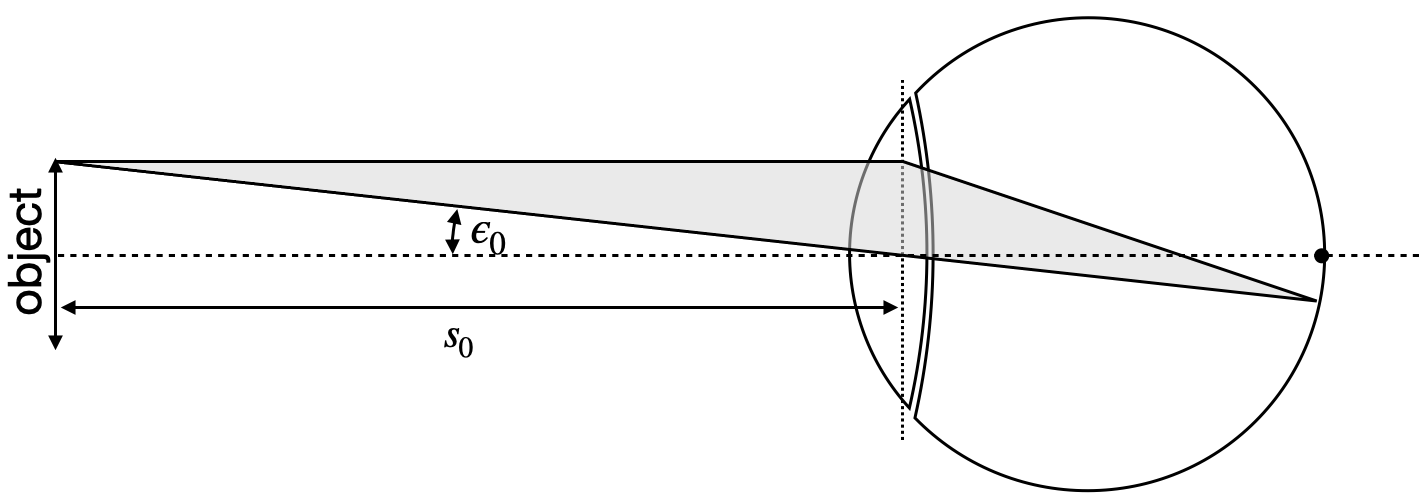
\includegraphics[width=0.8\linewidth,height=\textheight,keepaspectratio]{geometrical-optics/img/relaxed_eye.png}

}

\caption{\label{fig-relaxed-eye}Diagram of a relaxed eye focusing on a
distant object.}

\end{figure}%

history \textbar grep git

Understanding these concepts is crucial for diagnosing vision problems
and designing appropriate corrective measures, whether through
eyeglasses, contact lenses, or surgical interventions.

\subsection{Magnification}\label{magnification}

Having discussed the basic structure and function of the human eye, we
now turn to how optical instruments can enhance our vision. Instead of
calculating the magnification of optical instruments from object and
image distances, we introduce a more relevant measure: the
\textbf{angular magnification}.

The angular magnification, V, is defined as the ratio of the angle
subtended by the image when viewed through the instrument to the angle
subtended by the object when viewed with the naked eye at the near
point. It is given by:

\[
V=\frac{\tan(\epsilon)}{\tan(\epsilon_0)}\approx \frac{\epsilon}{\epsilon_0}
\]

where: - ε is the angle subtended by the image at the eye when viewed
through the instrument - ε₀ is the angle subtended by the object when
viewed with the naked eye at the near point

This concept is crucial in understanding how optical instruments like
telescopes and microscopes enhance our vision. Angular magnification
effectively increases the apparent size of objects by increasing the
angle at which they are viewed. This measure is particularly useful as
the actual image size is often not directly accessible or relevant to
the viewer's experience.

\chapter{Optical Instruments}\label{optical-instruments-1}

Optical instruments now combine a number of optical elements or even
consist only out of a single one as in the case of the magnifying glass
or the eye.

\section{Magnifying Glass}\label{magnifying-glass}

A magnifying glass has several applications. First of all, it allows to
see objects with details that would otherwise be too small to be
observed with the eye even of the eye lens can accommodate to the
distances. Such magnifying glasses are also used in microscopes as the
so-called \textbf{eye-piece} as we will later see in the section on
microscopes.

Consider the sketch below. The sketch shows an object of a size \(A\)
which is at a distance of \(s_0\) from the eye. The object makes an
angle \(\epsilon_0\) with the optical axis. If we insert now a lens into
the space between object and eye and the lens is positioned in a way
that it is exactly at a distance \(f\) (the focal distance of the lens)
from the object then we are able to observe the object under a different
angle \(\epsilon\).

\begin{figure}[H]

{\centering 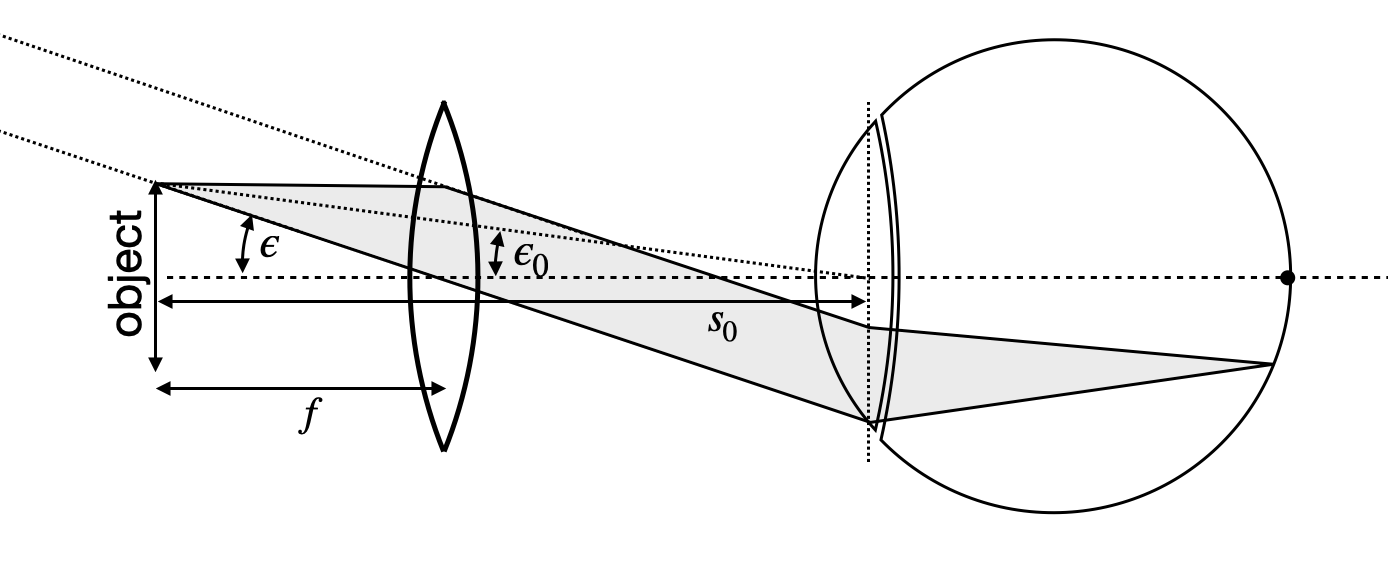
\includegraphics[width=0.6\linewidth,height=\textheight,keepaspectratio]{geometrical-optics/img/magnifying_glass_focal.png}

}

\caption{Magnifying glass at the focal distance.}

\end{figure}%

The magnification of this magnifying glass can the be calculated from
the angles \(\epsilon\approx A/f\) and \(\epsilon_0\approx A/s_0\):

\[
V=\frac{\tan(\epsilon)}{\tan(\epsilon_0)}\approx \frac{\epsilon}{\epsilon_0}=\frac{A}{f}\frac{s_0}{A}=\frac{s_0}{f}.
\]

The angular magnification is, thus, just given by the ratio of the clear
visual range to the focal distance of the lens. If the focal distance
\(f\) becomes much smaller than \(s_0\), large magnifications are
possible.

A second very useful effect is that when the object is placed inside the
focal distance from the lens, the eye images a virtual image at infinite
distance to the retina (see sketch). This means the eye muscle can stay
relaxed when observing the object, while it would otherwise probably
have to accommodate to the distance.

Yet, placing the object at exactly the focal distance is rather tedious
when holding the magnifying glass by hand. If the object is now placed
inside the focal distance of the magnifying glass, we may also calculate
a magnification in this case knowing the virtual image size \(B\)
created in this case (see sketch below)

\begin{figure}[H]

{\centering 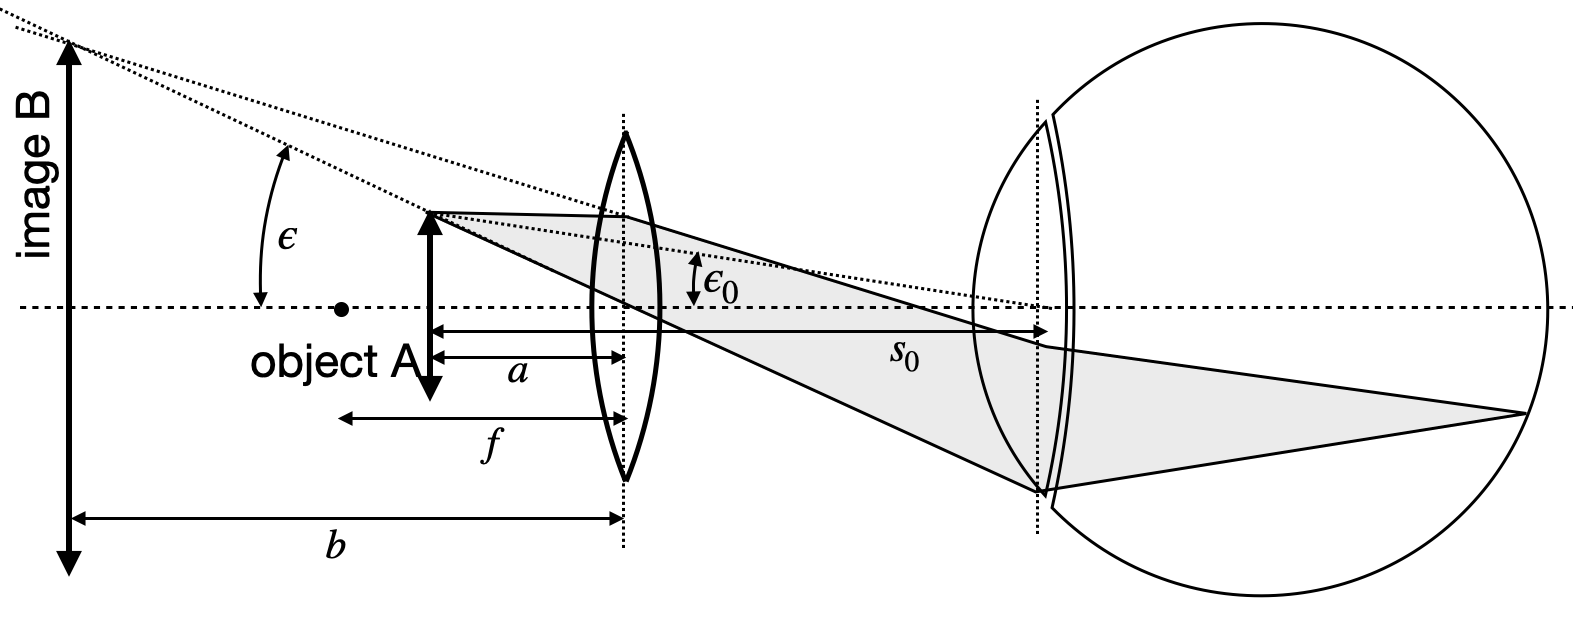
\includegraphics[width=0.6\linewidth,height=\textheight,keepaspectratio]{geometrical-optics/img/inside_focus.png}

}

\caption{Magnifying glass for an object inside the focal range of the
lens.}

\end{figure}%

If \(a\) is the distance of the object from the principle plane of the
magnifying glass and \(b\) and \(B\) are the distance and the size of
the virtual image, respectively, we obtain

\[
V=\frac{\tan(\epsilon)}{\tan(\epsilon_0)}\approx \frac{\epsilon}{\epsilon_0}=\frac{B}{b}\frac{s_0}{A}=\frac{s_0}{a}.
\]

Using the imaging equation

\[
\frac{1}{f}=\frac{1}{a}+\frac{1}{b}
\]

we may finally arrive at

\[
V=\frac{s_0(b-f)}{b\,f}
\]

in this case. If we place the virtual image directly at the clear visual
range, i.e., \(b=-s_0\), we find

\[
V=\frac{s_0}{f}+1.
\]

\chapter{Lens Systems and Optical
Instruments}\label{lens-systems-and-optical-instruments}

\subsection{Lens Systems}\label{lens-systems}

Most of the optical instruments consist of multiple lenses that are used
to image objects or to magnify them. They are combined at distances,
which are either larger or smaller than the sum of their focal
distances. The image below shows for example an artifical image of a
lens system contained in a single microscope objctive lens, where you
see multiple elements e.g.~doublets and triplets of lenses. These
elements as joined objects may considerably improve the performance of
the optics, e.g.~correct for imaging errors.

\begin{longtable}[]{@{}l@{}}
\toprule\noalign{}
 \\
\midrule\noalign{}
\endhead
\bottomrule\noalign{}
\endlastfoot
\textbf{Fig.:} System of of lenses inside a microscope objective
lens. \\
\end{longtable}

We will consider first a pair of two bi-convex lenses that are at a
distance \(D>f_1+f_2\)m where \(f_1\) and \(f_2\) are their focal
distances.

\begin{longtable}[]{@{}
  >{\raggedright\arraybackslash}p{(\linewidth - 0\tabcolsep) * \real{1.0000}}@{}}
\toprule\noalign{}
\begin{minipage}[b]{\linewidth}\raggedright
\end{minipage} \\
\midrule\noalign{}
\endhead
\bottomrule\noalign{}
\endlastfoot
\textbf{Fig.:} System of two bi-convex lenses at a distance larger than
the sum of their focal distances. \\
\end{longtable}

Here the first lens creates an image at a position

\[b_1=\frac{a_1 f_1}{(a_1-f_1)}\]

Accordingly the object distance for lens 2 is then \(a_2=D-b_1\).

The second lens then images this intermediate object into

\[b_2=\frac{a_2 f_2}{a_2-f_2}=\frac{(D-b_1) f_2}{D-b_1-f_2}\]

from which we can finally calculate the image location and also size
with the help of \(b_1\).

Instead of doing a lengthy transformation I would like to draw your
attention to a simple method which arises from the linearization of
Snells law. This is called \textbf{matrix optics}. Matrix optics relates
the outgoing angle \(\theta_2\) and height \(y_2\) of an optical element
to its incident angle \(\theta_1\) and \(y_1\) via a matrix operation.
Let's have a look at an example of a bi-convex lens with a focal length
\(f\). An incident ray is then expressed by a vector

\[\begin{bmatrix}
y_1\\
\theta_1
\end{bmatrix}\]

which is converted by the lens into an outgoing ray vector

\[\begin{bmatrix}
y_2\\
\theta_2
\end{bmatrix}\]

If you have two 2D vectors which you want to transform by a linear
operation into each other, then the transformation can be described by a
2x2 matrix, which is given for a lens with

\[\begin{bmatrix}
A & B\\
C & D
\end{bmatrix}
=
\begin{bmatrix}
1 & 0\\
-\frac{1}{f} & 1
\end{bmatrix}
\]

Similarly we can also define a free space propagation matrix for a
propagation by a distance \(D\), which is

\[\begin{bmatrix}
A & B\\
C & D
\end{bmatrix}
=
\begin{bmatrix}
1 & D\\
0 & 1
\end{bmatrix}
\]

The propagation of light through two lenses, which are seprarated by a
distance \(D\) is then the product of two matrices for the lenses and
one for the free space. The transformation then in addition requires to
multiply from the right side the incdent vector and we obtain on the
left side the outgoing ray vector.

\[\begin{bmatrix}
y_2\\
\theta_2\\
\end{bmatrix}
=
\begin{bmatrix}
1 & 0\\
-\frac{1}{f_2} & 1 \\
\end{bmatrix}
\begin{bmatrix}
1 & D\\
0 & 1
\end{bmatrix}
\begin{bmatrix}
1 & 0\\
-\frac{1}{f_1} & 1
\end{bmatrix}
\begin{bmatrix}
y_1\\
\theta_1
\end{bmatrix}\]

If you multiply the 2x2 matrices with each other, you will obtain a new
2x2 matrix with a matrix element \(C\), which should correspond to the
effective focal length of that system. This is the case since the
element \(C=-\frac{1}{f}\)

The result of that calculation is

\[\frac{1}{f}=\frac{1}{f_1}+\frac{1}{f_2}-\frac{D}{f_1 f_2}\]

which gives the effective focal length of two bi-convex lenses at a
distance \(D\).

Following this equation the inverse of the total focal length of the
combined lenses is just the sum of its inverse focal distances minus a
term, which depends on the distance of the two lenses. If this distance
is small as compared to the focal length, i.e.~the lenses are close to
each other, the total inverse focal is just given by the first two
terms. The inverse focal distances characterize the refractive power of
a lens. The larger the invserse value, the smaller is the focal
distance. This refractive power is commonly measured in the unit
\textbf{diopter}. One diopter corresponds to \textbf{1 dpt=1
\(m^{-1}\)}.

The image above shows also, that in the case of the combined lenses and
a real inverted intermediate image, the final image will be upright
again. Thus, if the first lens has a magnification \(M_1=-b_1/a_1\) and
the second lens a magnification \(M_2=-b_2/a_2\) the total magnification
is the product, which is

\[M=\frac{b_1}{a_1}\frac{b_2}{a_2}\]

from which we may finally obtain with \(M=\frac{f}{f-a}\)

\[M=\frac{1}{1-\frac{a_1}{f_1}-\frac{a_1+D}{f_2}+\frac{a_1D}{f_1 f_2}}\]

For more than two lenses, there is a versatile framework called
\textbf{Matrix Optics}, which treats each optical element as a 2x2
matrix. This becomes possible as we derived earlier equations which were
linear in \(y\) and \(\theta\). A whole system of different lenses,
plates and other optical elements can thus be treated as a matrix
multiplication, which is quite useful.

\chapter{Optical Instruments}\label{optical-instruments-2}

\section{Microscope}\label{microscope}

\begin{tcolorbox}[enhanced jigsaw, breakable, toptitle=1mm, bottomrule=.15mm, colbacktitle=quarto-callout-note-color!10!white, title=\textcolor{quarto-callout-note-color}{\faInfo}\hspace{0.5em}{Historical Context of Microscope Development}, arc=.35mm, rightrule=.15mm, bottomtitle=1mm, opacityback=0, toprule=.15mm, coltitle=black, leftrule=.75mm, opacitybacktitle=0.6, colback=white, left=2mm, titlerule=0mm, colframe=quarto-callout-note-color-frame]

Optical Microscopy has a rich history of development, and is a very
important tool in the fields of biology, materials science, and
nanotechnology. Here are some key milestones in the history of
microscopy:

\textbf{Ancient Times - 13th Century: Simple magnifying glasses} - The
concept of magnification was known to ancient civilizations. - In the
13th century, Italian craftsmen created the first wearable glasses.

\textbf{1590: Compound Microscope} - Hans and Zacharias Janssen, Dutch
spectacle makers, created the first compound microscope.

\textbf{1665: Robert Hooke's ``Micrographia''} - Hooke published
detailed observations made with his improved compound microscope. - He
coined the term ``cell'' after observing cork tissue.

\textbf{1670s: Antonie van Leeuwenhoek's Single-Lens Microscopes} -
Developed high-quality single-lens microscopes with up to 270x
magnification. - First to observe and describe bacteria, yeast, and
other microorganisms.

\begin{figure}[H]

{\centering 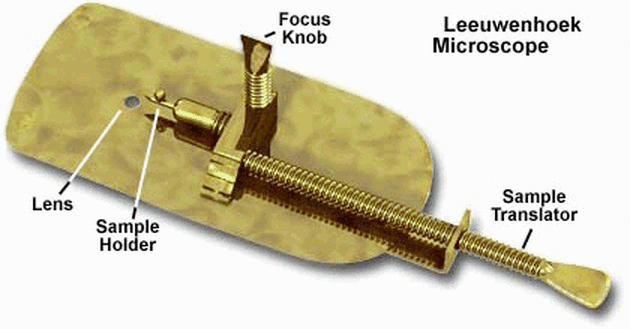
\includegraphics[width=0.5\linewidth,height=\textheight,keepaspectratio]{geometrical-optics/img/loewenhook.png}

}

\caption{Image of Leeuwenhoek's microscope}

\end{figure}%

\textbf{18th-19th Centuries: Achromatic Lenses} - Joseph Jackson Lister
developed achromatic lenses, reducing chromatic aberration.

\textbf{1830s: Ernst Abbe's Theoretical Work} - Formulated the Abbe Sine
Condition, crucial for modern lens design.

\textbf{Late 19th Century: Oil Immersion Lenses} - Allowed for higher
resolution in light microscopy.

\textbf{1931: Electron Microscope} - Ernst Ruska and Max Knoll developed
the first electron microscope.

\textbf{1950s-1960s: Phase Contrast and Fluorescence Microscopy} - Frits
Zernike invented phase contrast microscopy. - Development of
fluorescence microscopy techniques.

\textbf{1981: Scanning Tunneling Microscope} - Gerd Binnig and Heinrich
Rohrer invented the STM, allowing imaging at the atomic level.

\textbf{1980s-Present: Digital and Computational Microscopy} -
Integration of CCD cameras and digital imaging. - Development of
confocal microscopy, super-resolution techniques, and computational
methods like ptychography.

\end{tcolorbox}

In this section we will analyze the optical properties of microscopes
from the perspective of geometrical optics which explains image
formation. Yet, the key to the performance of a microscope is the
understanding provided by wave optics. We will discuss this in a later
section. The simplest form of a microscope consists of an objective lens
with a focal distance \(f_1\) and a magnifying glass called eye-piece
with a focal length \(f_2\). In this system of two lenses (which are
itself systems of lenses in modern microscopes, see below),

\begin{figure}[H]

{\centering 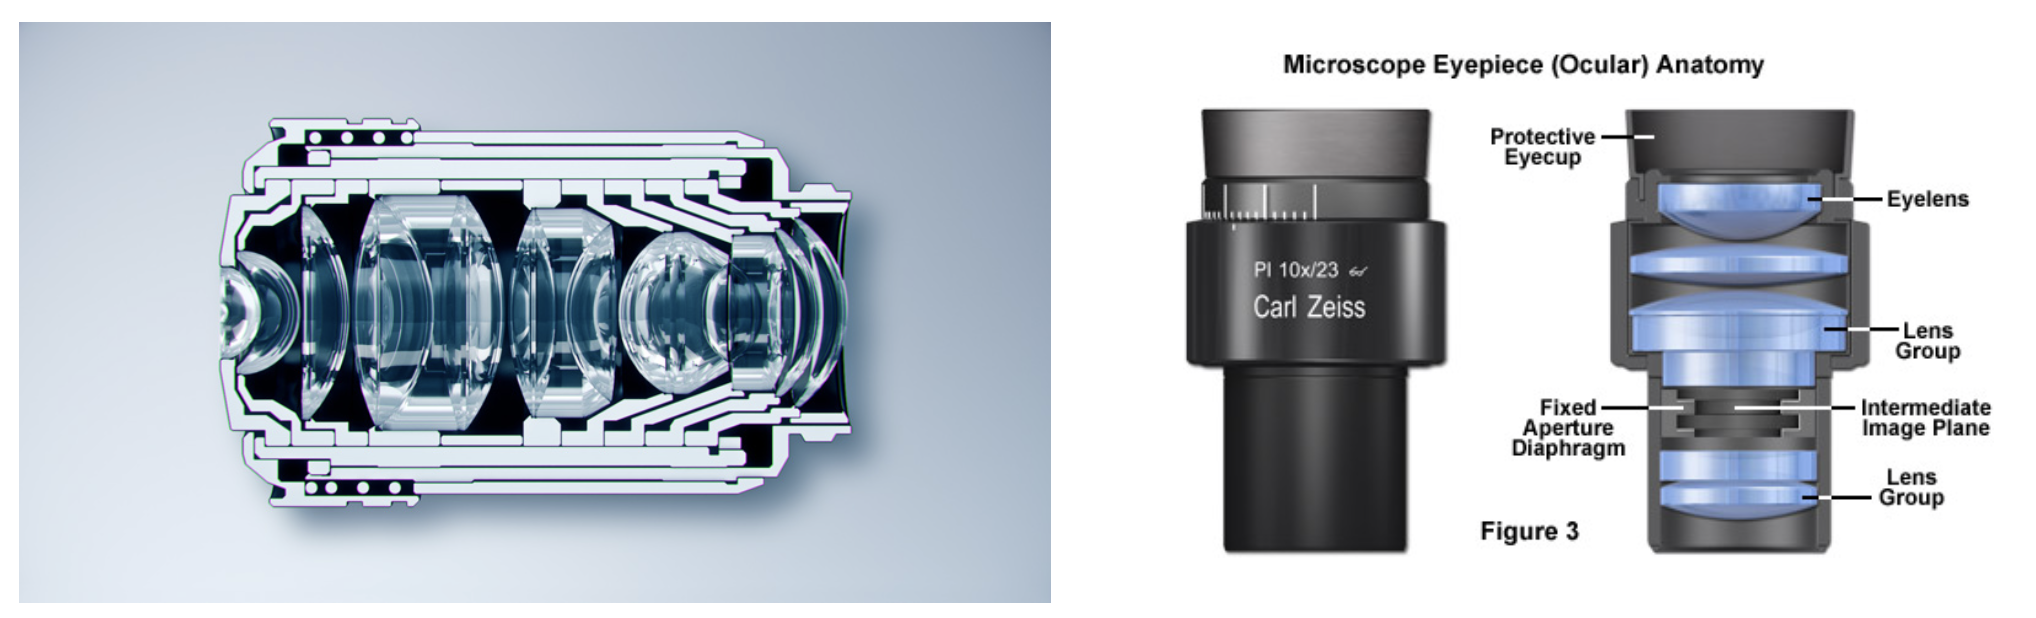
\includegraphics[width=0.6\linewidth,height=\textheight,keepaspectratio]{geometrical-optics/img/microscopy_lenses.png}

}

\caption{\textbf{Fig.:} Cut through a microscope objective lens (left)
and an eye-piece.}

\end{figure}%

the object is placed at a distance \(f_1< a_1<2f_1\) from the objective
lens creating a real and reversed image at a distance \(b_1\) behind the
lens. This reversed image is observed by the eye through the eye-piece.
The image of the objective lens is thereby adjusted to appear at the
focal distance of the eye-piece.

\begin{figure}[H]

{\centering 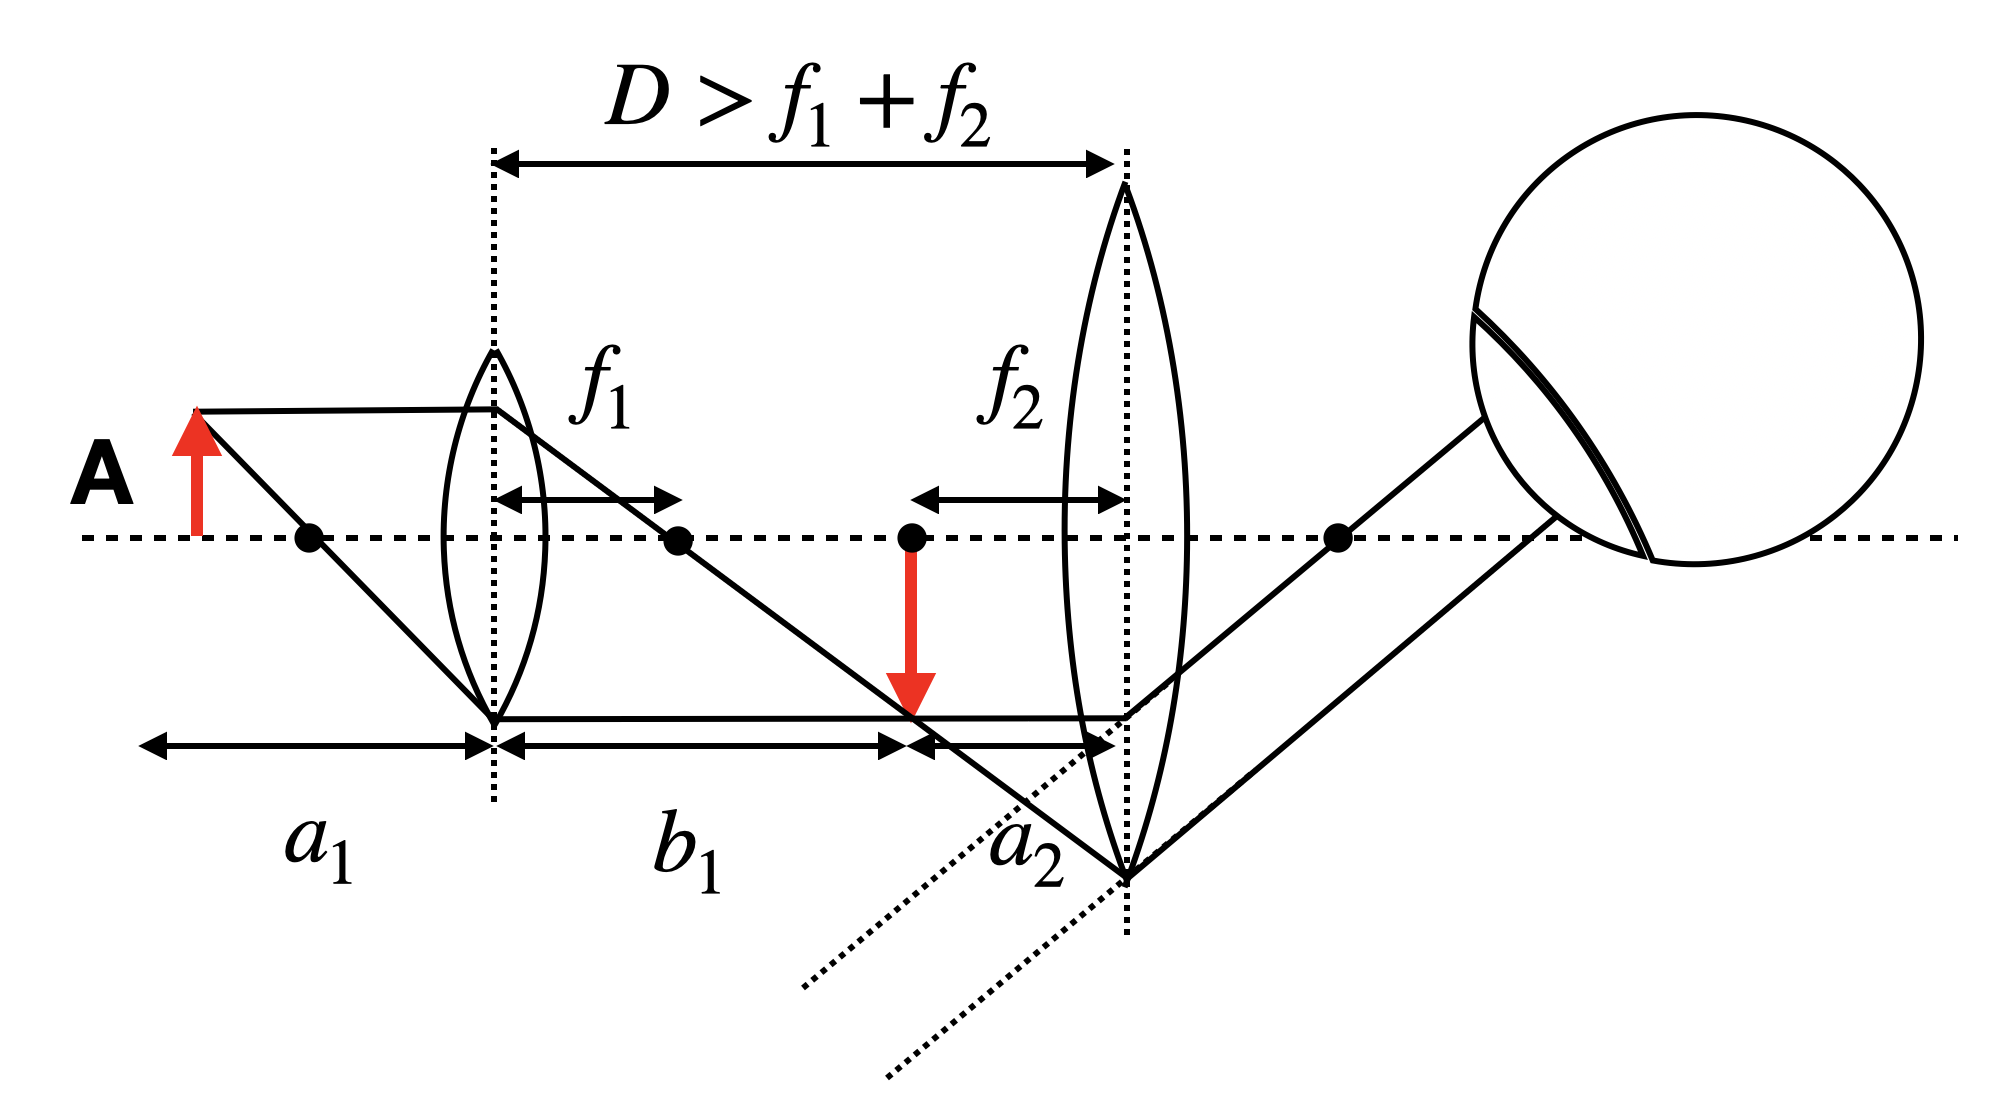
\includegraphics[width=0.6\linewidth,height=\textheight,keepaspectratio]{geometrical-optics/img/simple_microscope.png}

}

\caption{\textbf{Fig.:} Sketch of a simple microscope. The strange
object on the right is an eye.}

\end{figure}%

For this simple microscope system we may calculate first the
intermediate image position \(b_1\):

\[
\frac{1}{f_1}=\frac{1}{a_1}+\frac{1}{b_1}
\]

resulting in

\[
b_1=\frac{a_1 f_1}{a_1-f_1}.
\]

If we assume a \(\delta\) to be the distance of the object from the
focal point of the objective lens, we even find for
\(\delta \rightarrow 0\)

\[
b_1=\frac{a_1 f_1}{\delta}.
\]

The intermediate image of size \(B_1\) is now imaged by a magnifying
glass of focal distance \(f_2\). According to what we calculated
earlier, we have now the observation angle

\[
\tan(\epsilon)=\frac{B_1}{f_2}=\frac{Ab_1}{a_1 f_2}.
\]

If we observe the object of a size \(A\) and the clear visual distance
\(s_0\), it would cover an angle of

\[
\tan(\epsilon_0)=\frac{A}{s_0}
\]

and we may obtain the total angular magnification

\[
V=\frac{A b_1 s_0}{A a_1 f_2}=\frac{b_1 s_0}{a_1 f_2}.
\]

If we set the distance between the two lenses to \(D=b_1+f_2\) and
\(a_1\approx f_1\) then we obtain

\[
V=\frac{(D-f_2)s_0}{f_1 f_2}
\]

which says that the magnification is the result of the two focal length
\(f_1,f_2\).

\subsubsection{Modern microscopy}\label{modern-microscopy}

While the description above accurately represents the simplest
microscope design, contemporary microscopes employ more intricate light
paths and generally utilize what is known as \textbf{infinity corrected}
optics. This system incorporates an objective lens that projects images
of objects in the focal plane to infinity. Such an objective lens is
invariably paired with a secondary lens, called the \textbf{tube lens}.
Together, these lenses are engineered to provide a magnification level
that is specified on the objective lens housing.

\begin{figure}[H]

{\centering 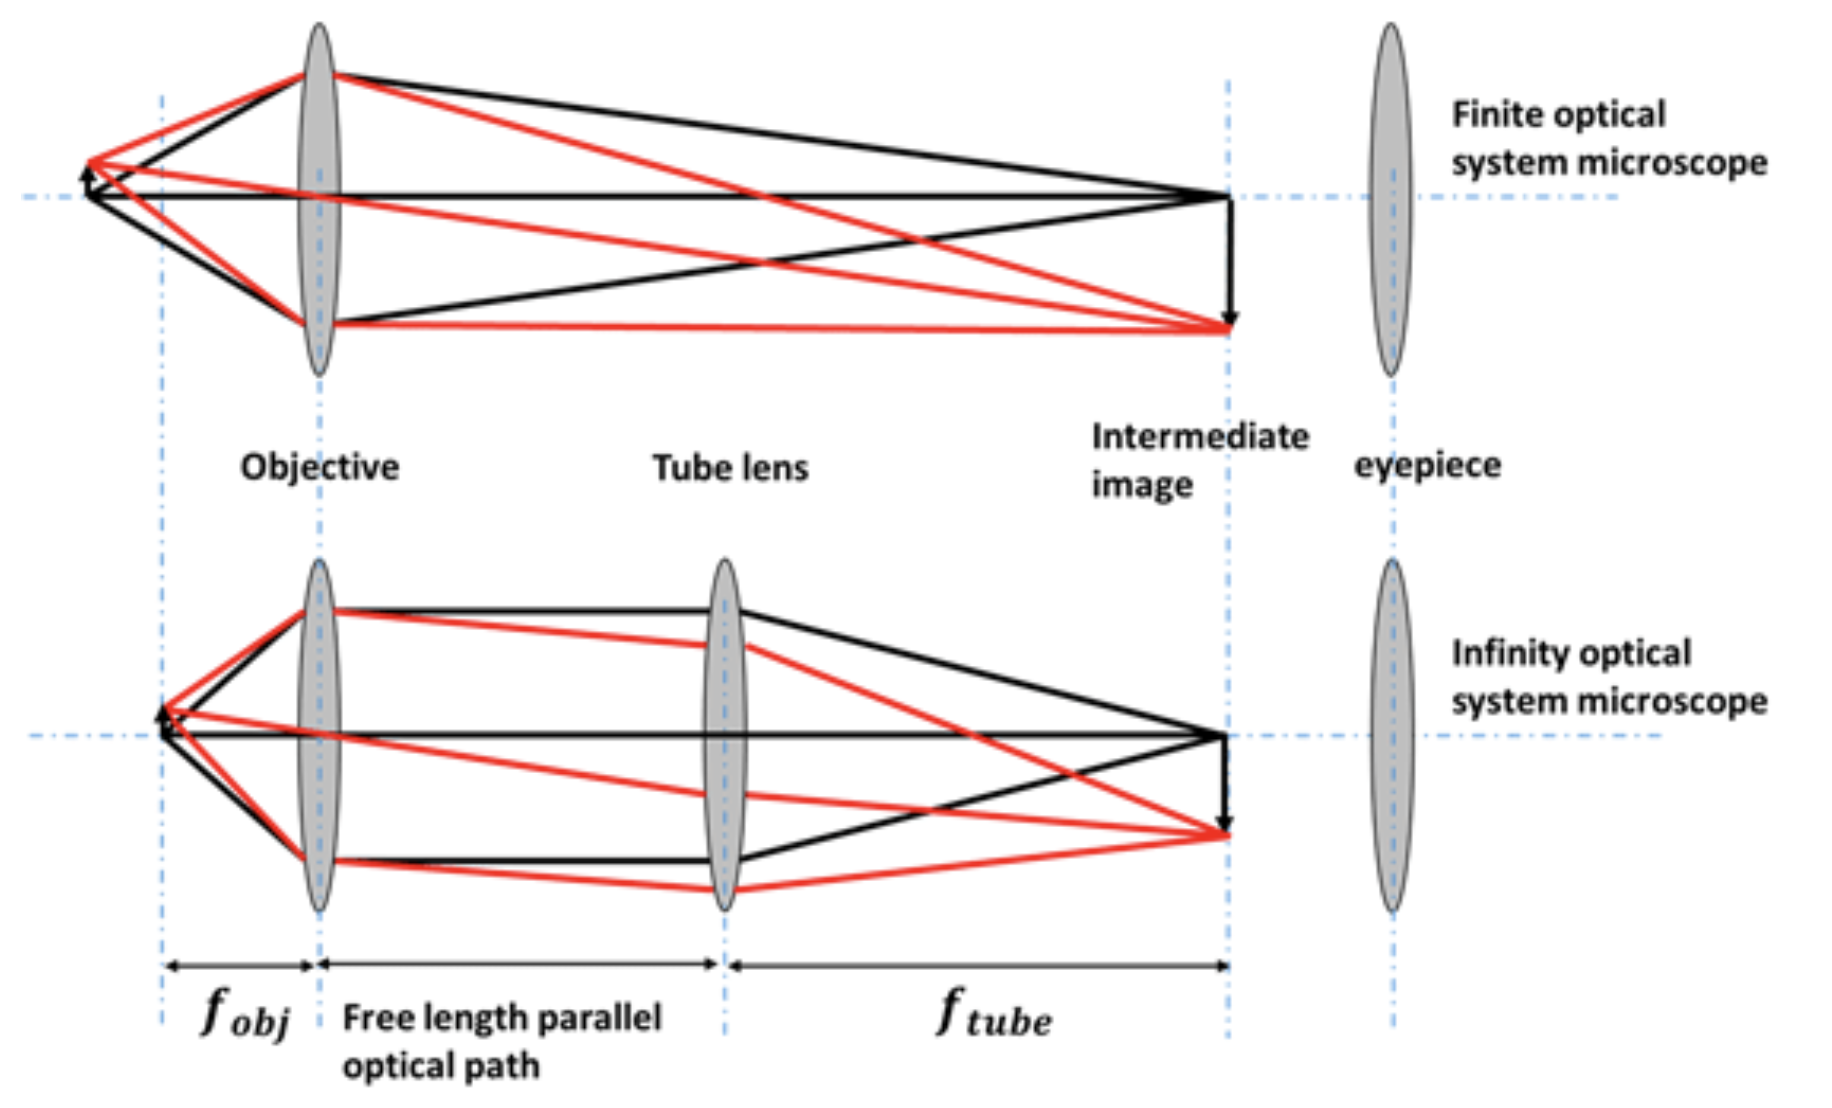
\includegraphics[width=0.6\linewidth,height=\textheight,keepaspectratio]{geometrical-optics/img/infinity_optics.png}

}

\caption{\textbf{Fig.:} Infinity optics vs.~normal microscopy optics.}

\end{figure}%

Infinity optics allows you to have a free length with a parallel optical
path where you can insert optical elements. There is no fixed tube
length as in the case sketched above, where the distance of the
intermediate image has to be considered. Therefore, it has tremendous
technical advantages. Common optical microscopes are further today
coupled to CCD cameras to record images digitally. Yet, an eye-piece may
still be available in many cases. The sketch below shows the light path
for a simple fluorescence microscope recording fluorescence images with
a camera.

\begin{figure}[H]

{\centering 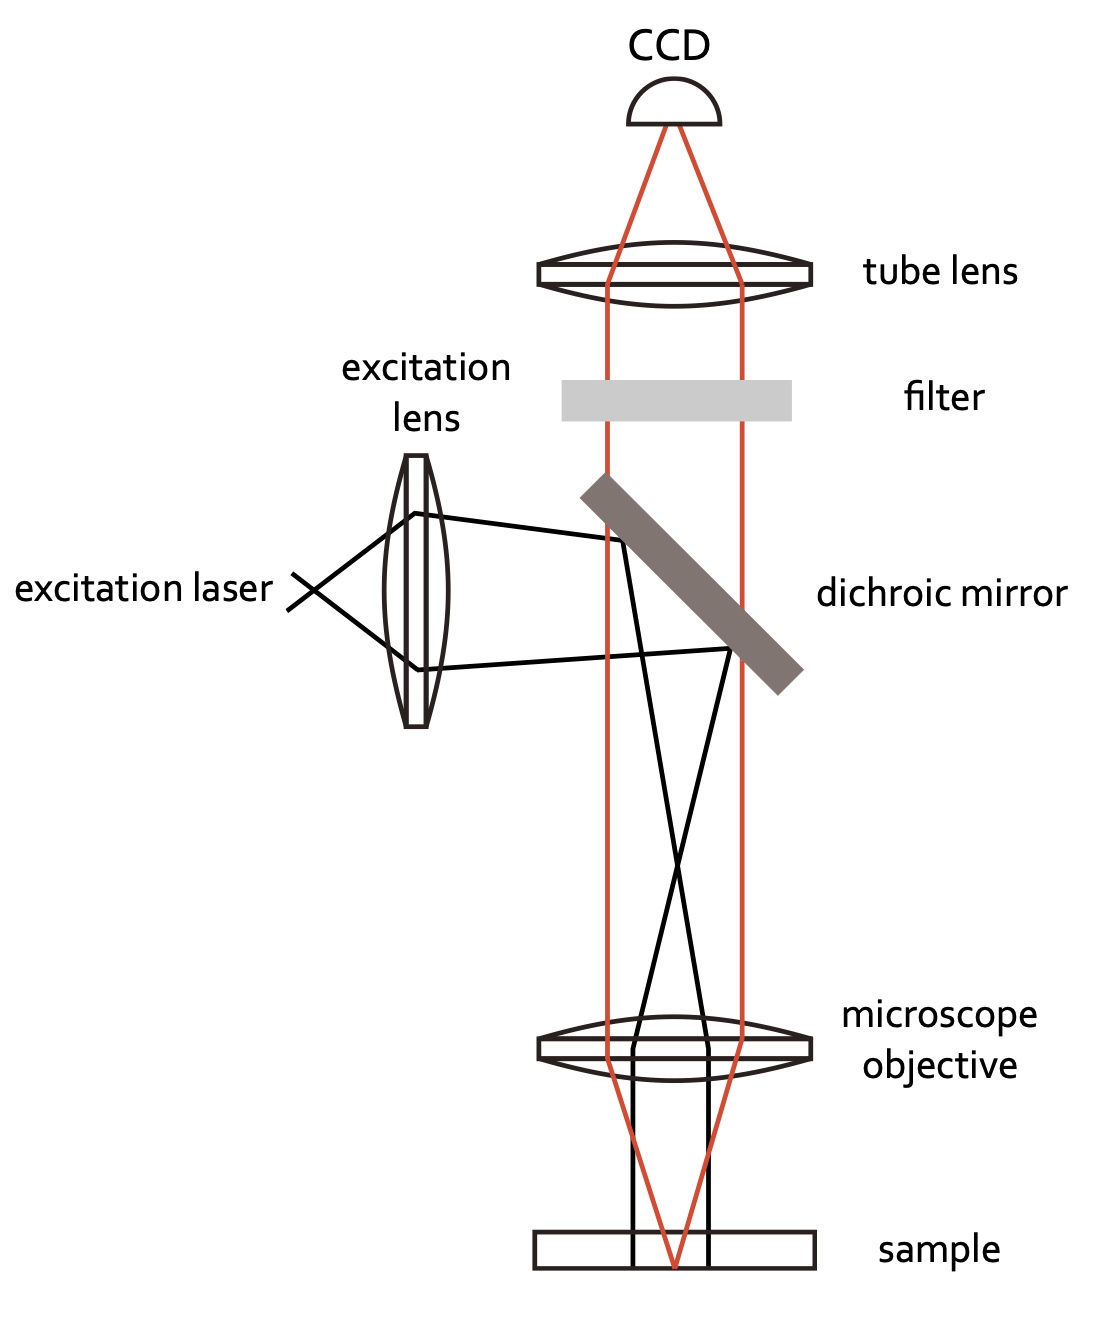
\includegraphics[width=0.4\linewidth,height=\textheight,keepaspectratio]{geometrical-optics/img/fluorescence_micr.png}

}

\caption{\textbf{Fig.:} Simple fluorescence microscope.}

\end{figure}%

\subsubsection{Digital Microscopy}\label{digital-microscopy}

The possibility to digitally record images creates endless possibilities
to computationally enhance and combine images. Nowadays the field of
optics is one of the fastest developing fields in physics with numerous
new techniques appearing every week. In this field of imaging methods of
machine learning also play an increasingly important role. While I'm not
ablields in physics with numerous new techniques appearing every week.
In this field of imaging methods of machine learning also play an
increasingly important role. While I am not able to refer to all
possible optical microscopy techniques he to refer to all possible
optical microscopy techniques here, I will exemplarily show some data
from the Waller group at Berkley using computational methods to enhance
the resolution by keeping at the same time a large field of view for
imaging. This technique is called \textbf{ptychography} and can be
understood if you consider Fourier Optics (a field of optics describing
ligh propagation in terms Fourier transforms).

\begin{figure}[H]

{\centering 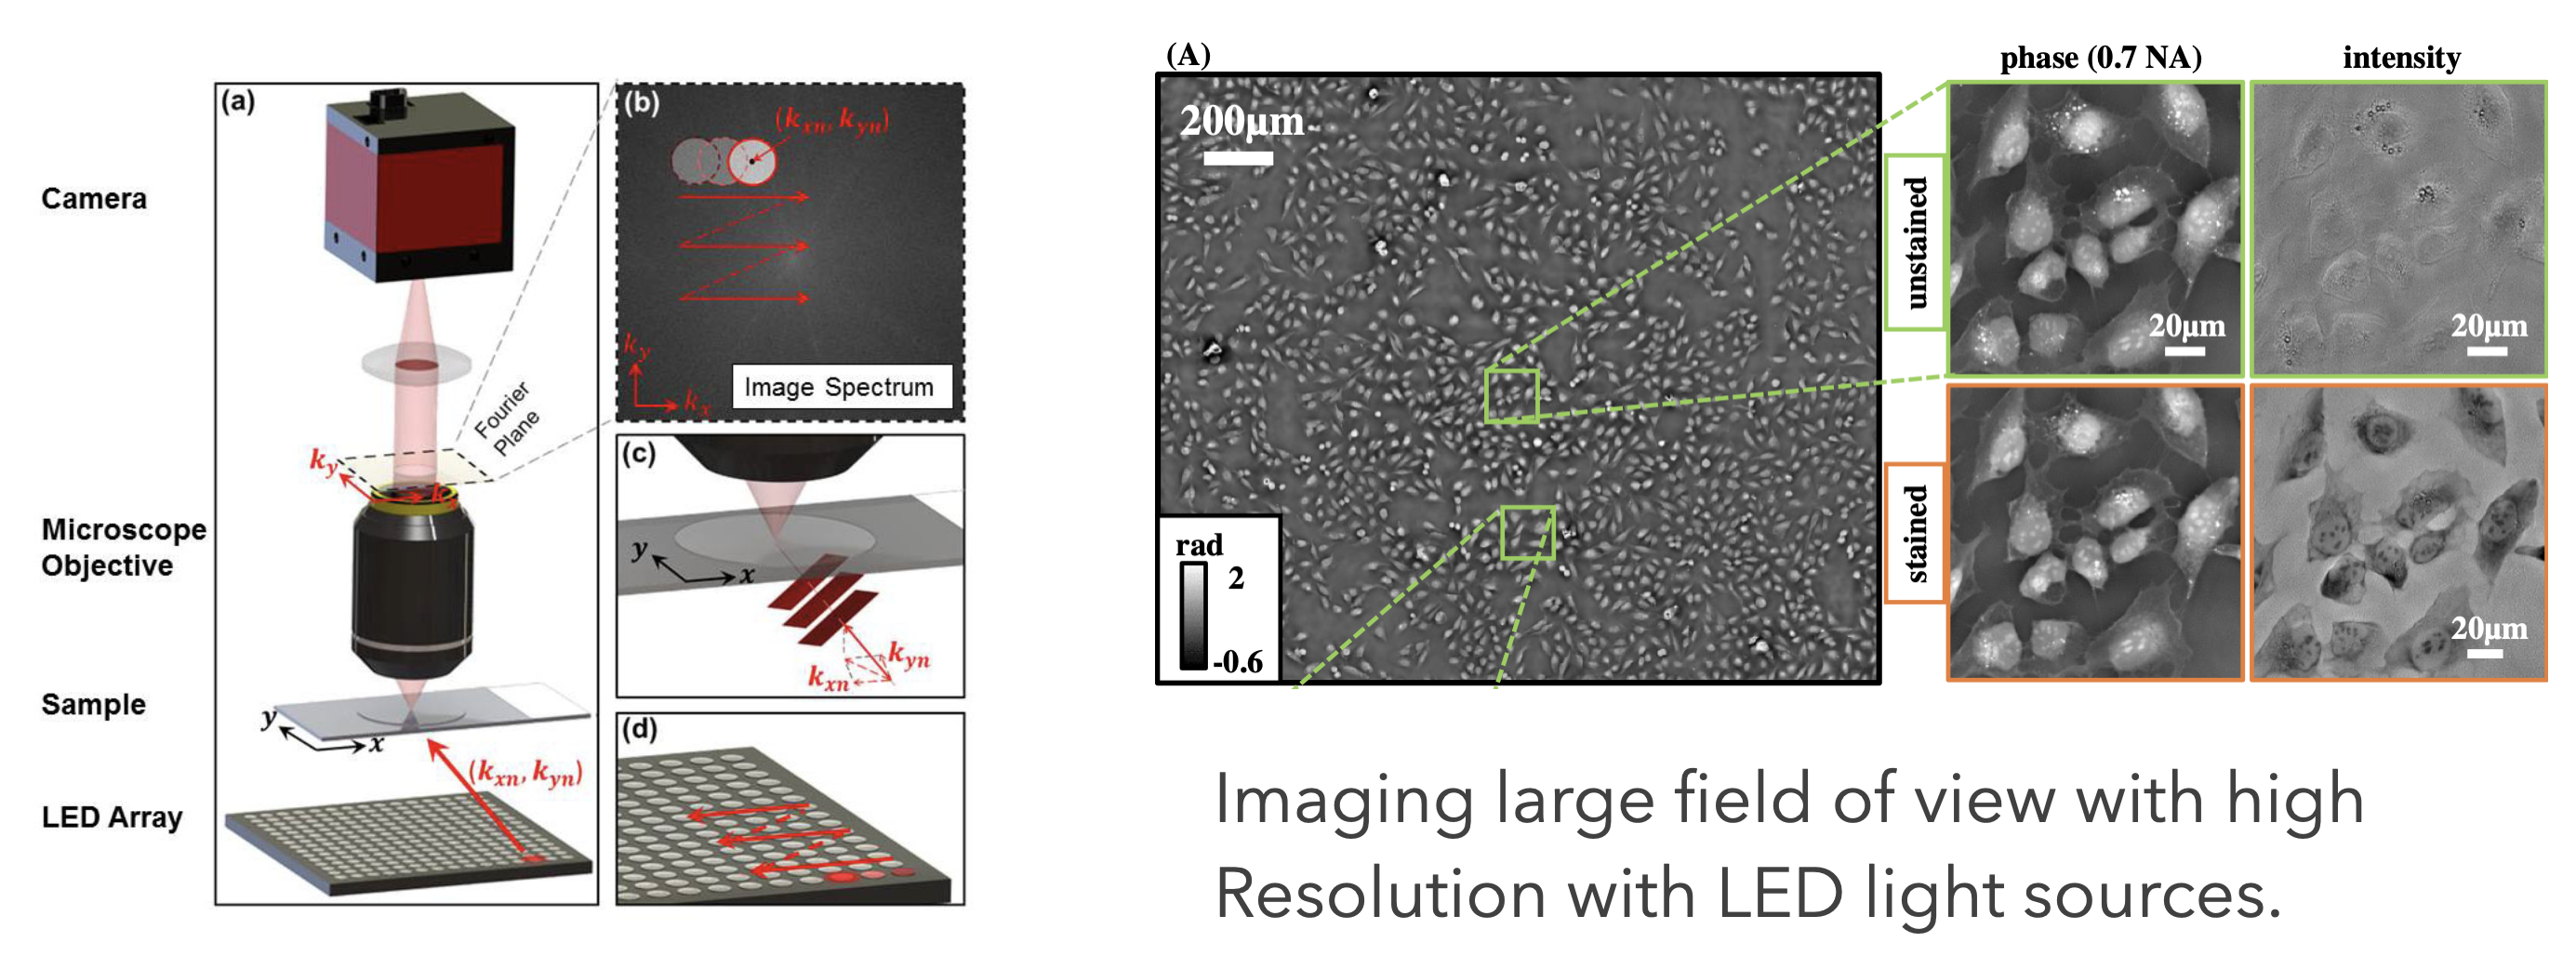
\includegraphics[width=1\linewidth,height=\textheight,keepaspectratio]{geometrical-optics/img/ptychography.png}

}

\caption{\textbf{Fig.:} Ptychographic imaging with LED arrays.}

\end{figure}%

There is a massive amount of other techniques with increadible images
being generated. Have a look around.

\begin{tcolorbox}[enhanced jigsaw, breakable, toptitle=1mm, bottomrule=.15mm, colbacktitle=quarto-callout-note-color!10!white, title=\textcolor{quarto-callout-note-color}{\faInfo}\hspace{0.5em}{Advanced Microscopy Techniques}, arc=.35mm, rightrule=.15mm, bottomtitle=1mm, opacityback=0, toprule=.15mm, coltitle=black, leftrule=.75mm, opacitybacktitle=0.6, colback=white, left=2mm, titlerule=0mm, colframe=quarto-callout-note-color-frame]

While traditional light microscopy has been invaluable, it's limited by
the diffraction of light, restricting resolution to about 200 nm as will
be discussed in a later part of this course. Modern techniques have
pushed beyond this limit, revolutionizing our ability to visualize
microscopic structures.

\begin{figure}[H]

{\centering 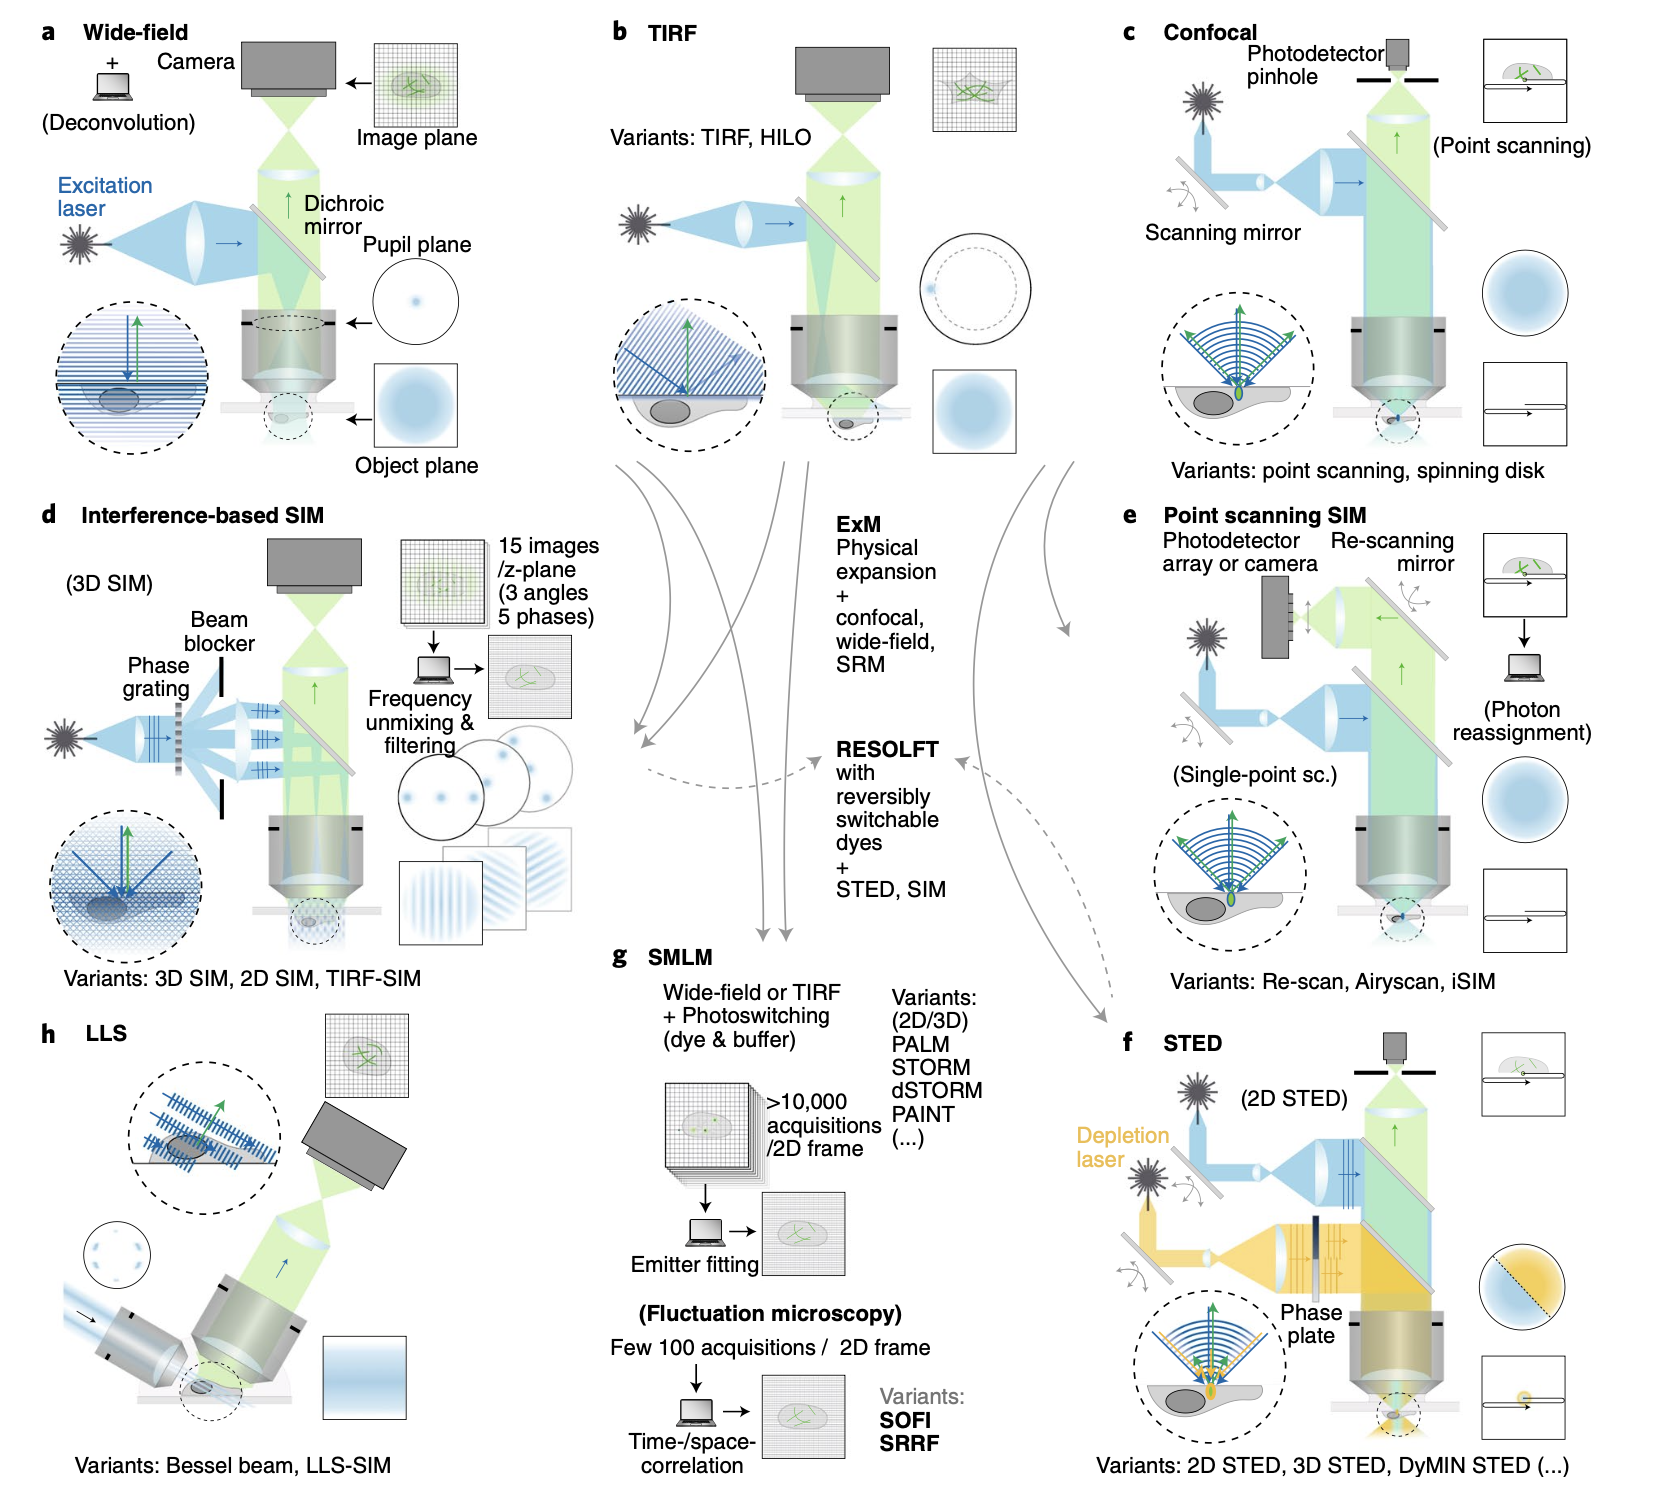
\includegraphics[width=0.8\linewidth,height=\textheight,keepaspectratio]{geometrical-optics/img/SuperRes.png}

}

\caption{Super resolution Imaging Methods Overview (Schermelleh, L. et
al.~Super-resolution microscopy demystified. Nat. Cell Biol. 21, 72--84
(2019))}

\end{figure}%

\subsection{Confocal Microscopy}\label{confocal-microscopy}

Confocal microscopy uses point illumination and a pinhole in an
optically conjugate plane in front of the detector to eliminate
out-of-focus signal.

\begin{figure}[H]

{\centering 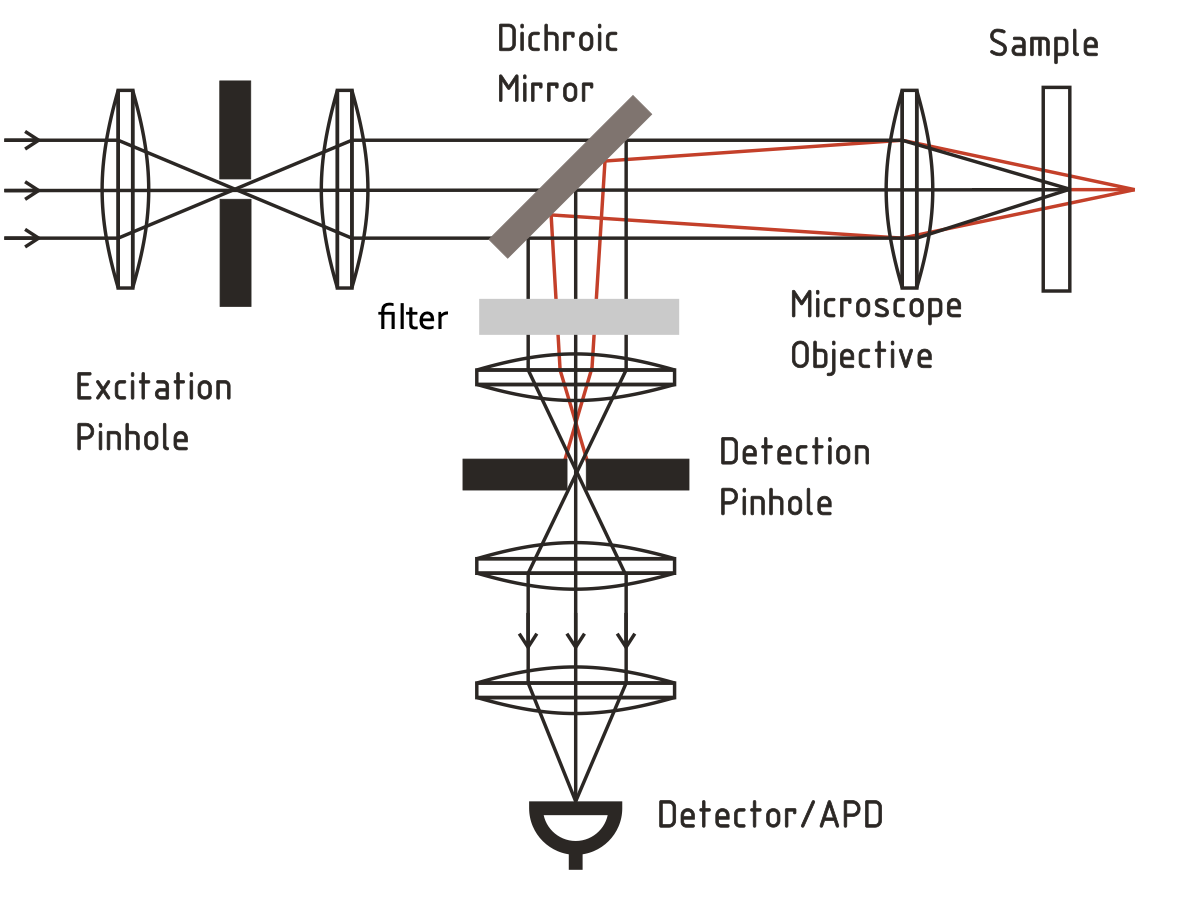
\includegraphics[width=0.6\linewidth,height=\textheight,keepaspectratio]{geometrical-optics/img/confocal.png}

}

\caption{Confocal Microscope.}

\end{figure}%

\begin{itemize}
\tightlist
\item
  \textbf{Key Features:}

  \begin{itemize}
  \tightlist
  \item
    Improved optical resolution and contrast
  \item
    Ability to collect serial optical sections from thick specimens
  \item
    Widely used in biological sciences
  \end{itemize}
\item
  \textbf{Overcoming Limitations:}

  \begin{itemize}
  \tightlist
  \item
    Eliminates background information away from the focal plane
  \item
    Allows for 3D reconstruction of samples
  \end{itemize}
\end{itemize}

\subsection{Examples for Super-Resolution Microscopy
Techniques}\label{examples-for-super-resolution-microscopy-techniques}

Super-resolution techniques bypass the diffraction limit, achieving
resolutions down to tens of nanometers.

\begin{enumerate}
\def\labelenumi{\arabic{enumi}.}
\tightlist
\item
  \textbf{Stimulated Emission Depletion (STED) Microscopy}

  \begin{itemize}
  \tightlist
  \item
    Uses two laser beams: one to excite fluorescent molecules, another
    to suppress fluorescence around the excitation spot
  \item
    \textbf{Overcoming Limitations:} Achieves resolution as fine as
    20-50 nm by precisely controlling which fluorophores are allowed to
    fluoresce
  \end{itemize}
\item
  \textbf{Photoactivated Localization Microscopy (PALM)}

  \begin{itemize}
  \tightlist
  \item
    Relies on selective activation and sampling of sparse subsets of
    photoactivatable fluorescent molecules
  \item
    \textbf{Overcoming Limitations:} Locates individual molecules with
    nanometer precision by isolating their signals over time
  \end{itemize}
\item
  \textbf{Stochastic Optical Reconstruction Microscopy (STORM)}

  \begin{itemize}
  \tightlist
  \item
    Similar to PALM, but uses photoswitchable fluorophores
  \item
    \textbf{Overcoming Limitations:} Achieves resolutions of
    \textasciitilde20 nm by precisely locating the centers of single
    fluorescent molecules
  \end{itemize}
\item
  \textbf{Structured Illumination Microscopy (SIM)}

  \begin{itemize}
  \tightlist
  \item
    Uses patterned illumination to create moiré fringes, which are
    computationally processed to reconstruct super-resolution images
  \item
    \textbf{Overcoming Limitations:} Doubles the resolution of
    traditional light microscopy to \textasciitilde100 nm
  \end{itemize}
\item
  \textbf{Superresolution Photothermal Infrared Imaging}

  \begin{itemize}
  \tightlist
  \item
    Superresolution photothermal infrared imaging is a novel technique
    that brings the advantages of superresolution microscopy to the
    infrared regime.
  \item
    \textbf{Overcoming Limitations:} Achieves resolutions of
    \textasciitilde300 nm for infrared imaging at wavelength of 10 µm by
    using photothermal lensing effects.
  \end{itemize}
\end{enumerate}

\end{tcolorbox}

\chapter{Telescopes}\label{telescopes}

Other than the microscope, the telescope is made to observe distant
objects, which would appear under a very small observation angle. This
can be achieved with different optical designs. The most common
telescopes are refracting telescopes, which use lenses to magnify the
angle under which the object is observed. The second type of telescopes
are reflecting telescopes, which use mirrors to magnify the angle under
which the object is observed.

\subsection{Refracting Telescopes}\label{refracting-telescopes}

The telescope is therefore made to magnify the angle under which the
object is observed. In the same way as a microscope, the telescope
consists of two lenses with the focal distances \(f_1,f_2\).

\begin{figure}[H]

{\centering 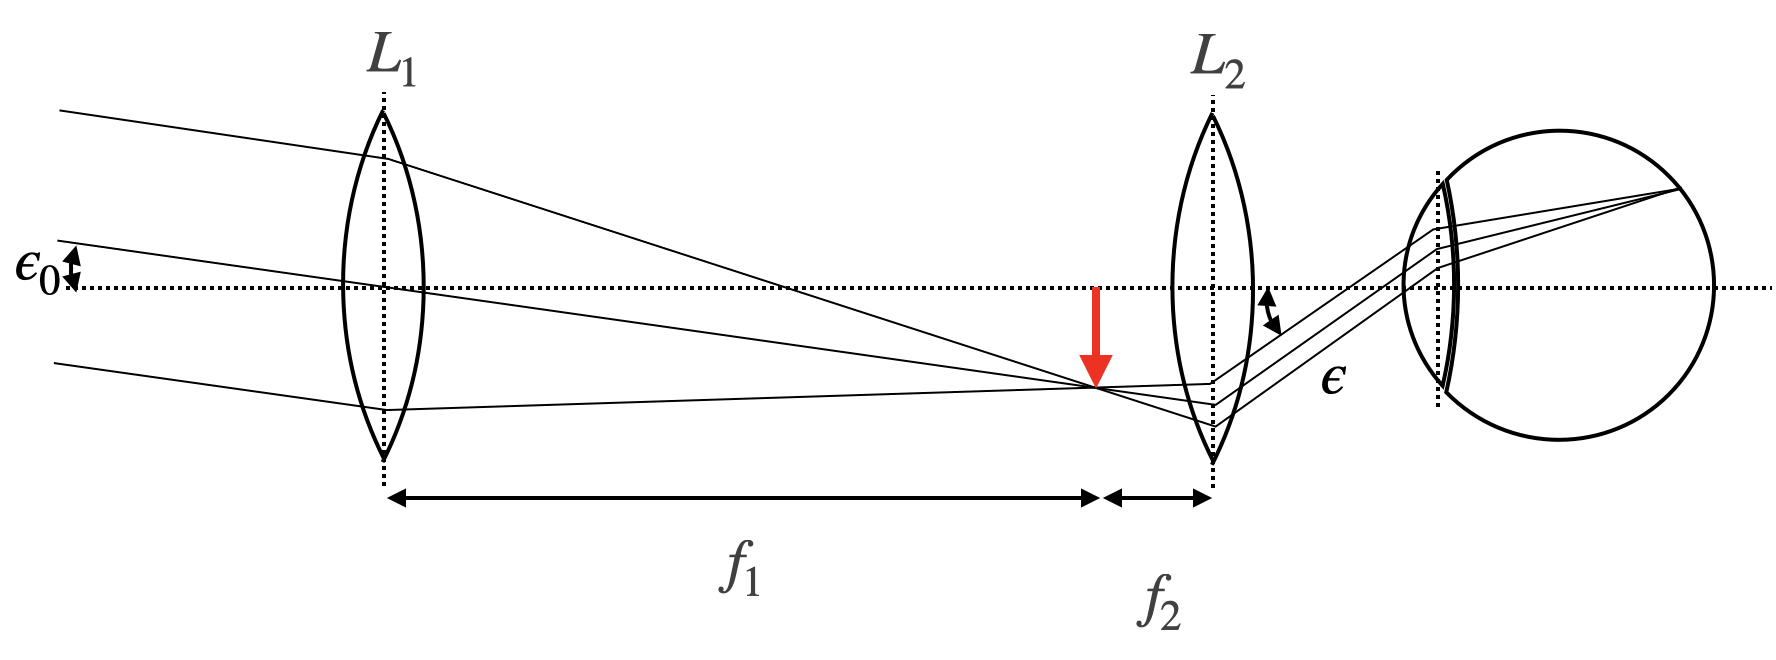
\includegraphics[width=0.6\linewidth,height=\textheight,keepaspectratio]{geometrical-optics/img/telescope.png}

}

\caption{Kepler telescope with two biconvex lenses, creating a reversed
image of distance objects.}

\end{figure}%

As indicated in the sketch above, the first lens generates an image at
the focal length of the first lens. This intermediate image is the
magnified by an eye-piece as well acting as a magnifying glass. We may
therefore apply the same kind of techniques as earlier for the
calculation of the angular magnification. The angle of observation for
the object of size \(D\) is given by

\[
2\epsilon_0=\frac{D}{f_1}
\]

while the angle of observation through the telescope is given as

\[
2\epsilon=\frac{D}{f_2}
\]

Correspondingly, the angular magnification is given by

\[
V=\frac{\epsilon}{\epsilon_0}=\frac{D}{f_2}\frac{f_1}{D}=\frac{f_1}{f_2}
\]

The magnification is therefore given by the ration of the focal length
of the entrance lens and the eye-piece. The above telescope is also
termed \textbf{astronomical telescope} or \textbf{Kepler telescope},
since it has been used for astromical observations. It creates an image
which is reversed.

A telescope with an upright image may be created with the help of a
concave lens. This type of telescope is called Galilei telescope and
obeyes the same magnification formula as above. Due to the fact that a
concave lens has a negative focal length, the total magnification will
be negative as well being indicative for an upright image.

\subsubsection{Light Gathering Power}\label{light-gathering-power}

While magnification is important for resolving details in celestial
objects, the ability to collect light is equally crucial for observing
faint astronomical objects. The light gathering power of a telescope is
determined by the area of its objective lens or primary mirror, which
scales with the square of the aperture diameter. A telescope with an
aperture diameter \(D\) collects light proportional to \(\pi D^2/4\).
This means that doubling the diameter of a telescope increases its light
gathering ability by a factor of four. For example, a telescope with a
200 mm aperture collects four times as much light as a 100 mm telescope,
making it possible to observe objects that are significantly fainter.

\begin{tcolorbox}[enhanced jigsaw, breakable, toptitle=1mm, bottomrule=.15mm, colbacktitle=quarto-callout-note-color!10!white, title=\textcolor{quarto-callout-note-color}{\faInfo}\hspace{0.5em}{Magnification vs.~Aperture}, arc=.35mm, rightrule=.15mm, bottomtitle=1mm, opacityback=0, toprule=.15mm, coltitle=black, leftrule=.75mm, opacitybacktitle=0.6, colback=white, left=2mm, titlerule=0mm, colframe=quarto-callout-note-color-frame]

While high magnification might seem desirable, it is the aperture size
that fundamentally limits what a telescope can observe. Magnifying a dim
image beyond what the aperture can support only results in a larger but
dimmer image. Professional observatories therefore prioritize large
apertures to maximize light collection.

\end{tcolorbox}

\subsubsection{Exit Pupil}\label{exit-pupil}

An important practical consideration when using a telescope is the exit
pupil, which is the diameter of the light beam that exits the eyepiece
and enters the observer's eye. The exit pupil diameter can be calculated
as the ratio of the objective diameter to the magnification:

\[
D_{exit} = \frac{D_{objective}}{V}
\]

For comfortable viewing, the exit pupil should ideally match the
diameter of the observer's eye pupil. The human eye pupil varies from
about 2 mm in bright light to 7 mm in dark-adapted conditions. If the
exit pupil is larger than the eye's pupil, some light is wasted. If it
is too small, the image may appear dim and the full aperture of the
telescope is not effectively utilized. This relationship shows that for
a given telescope, there is an optimal range of magnifications for
visual observation.

\begin{figure}[H]

{\centering 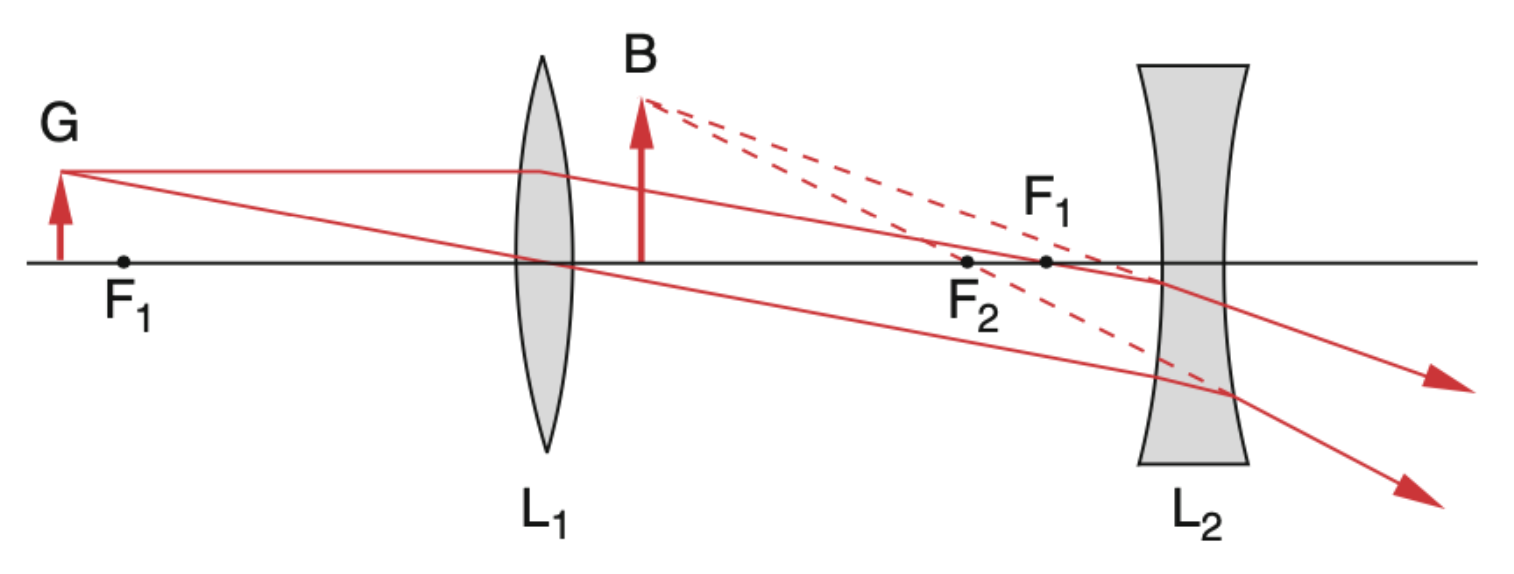
\includegraphics[width=0.6\linewidth,height=\textheight,keepaspectratio]{geometrical-optics/img/galilei.png}

}

\caption{Galilei telescope for imaging objects into upright images with
the help of a concave and a convex lens.}

\end{figure}%

\subsection{Reflecting Telescopes}\label{reflecting-telescopes}

Modern powerful telescopes also use mirrors instead of refracting
optical elements, as reflecting elements with nearly 100 percent
reflectivity can be built with a much smaller mass than large glass
elements. Such telescopes come in different setups. The one below is a
Cassegrain telescope, where a secondary convex miror is used for imaging
the intermediate image to the eye.

\begin{figure}

\begin{minipage}{0.50\linewidth}
\pandocbounded{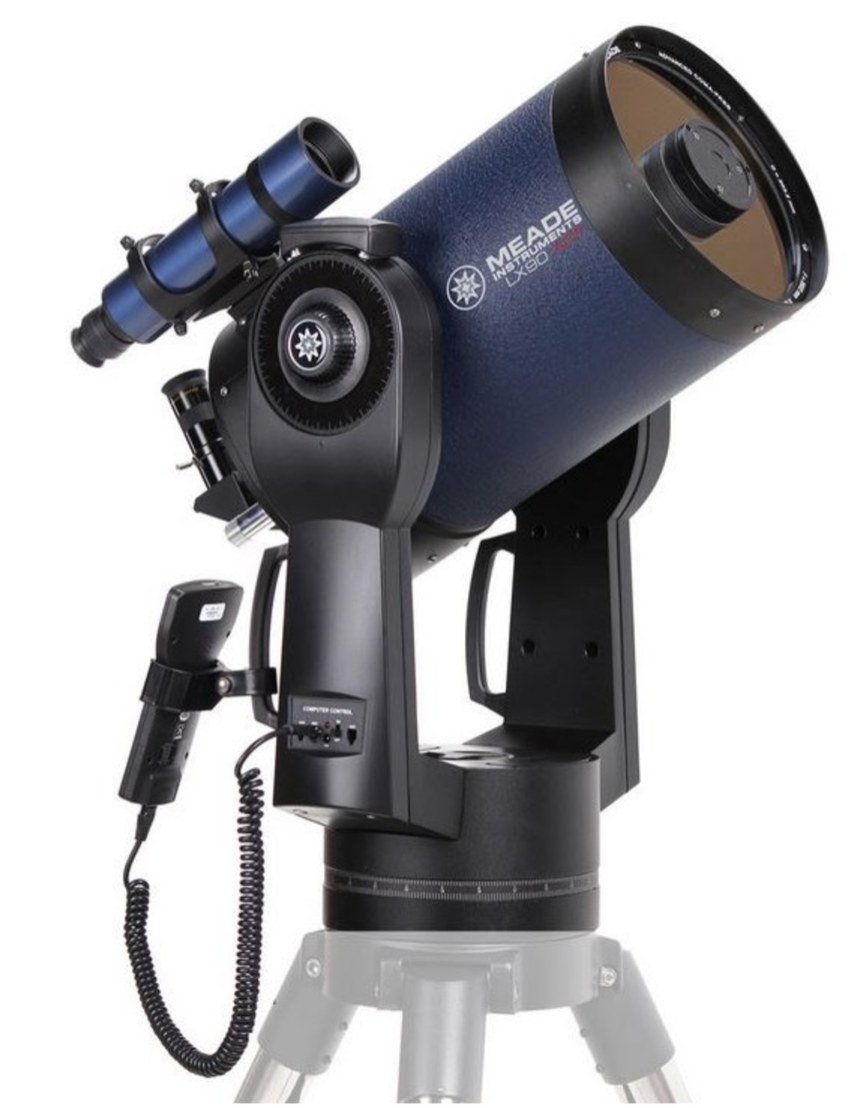
\includegraphics[keepaspectratio]{geometrical-optics/img/real_telescope.png}}\end{minipage}%
%
\begin{minipage}{0.50\linewidth}

\begin{figure}[H]

{\centering 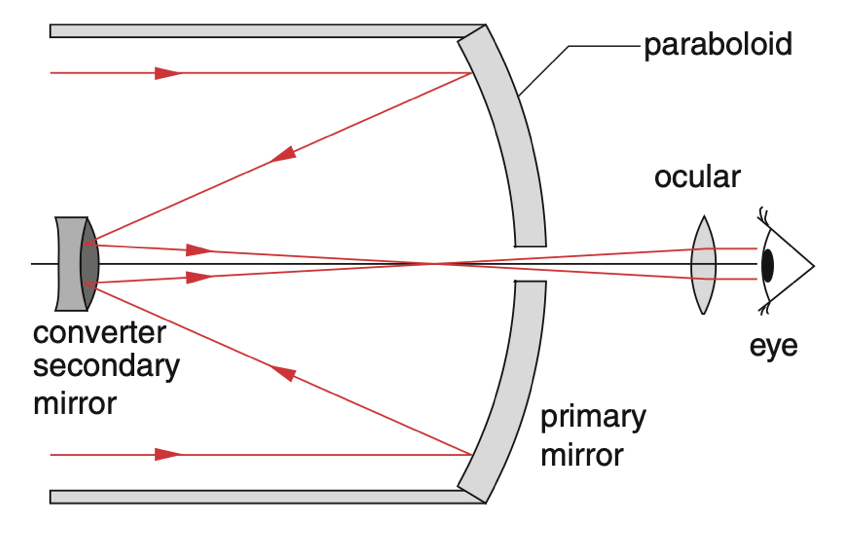
\includegraphics[width=1\linewidth,height=\textheight,keepaspectratio]{geometrical-optics/img/cassegrain.png}

}

\subcaption{Reflective optics is commonly used in modern high quality
telescopes for the advantage of weight. The image and sketch shows the
optics of a so-called Cassegrain telescope.}

\end{figure}%

\end{minipage}%

\end{figure}%

\subsubsection{Other Reflecting Telescope
Designs}\label{other-reflecting-telescope-designs}

Beyond the Cassegrain design, several other reflecting telescope
configurations are commonly used, each with its own advantages. The
\textbf{Newtonian telescope}, designed by Isaac Newton in 1668, is
perhaps the simplest reflecting telescope design. It uses a parabolic
primary mirror that reflects light to a small flat secondary mirror
positioned at 45 degrees near the front of the tube. This secondary
mirror directs the light to an eyepiece mounted on the side of the
telescope tube. The Newtonian design is popular among amateur
astronomers due to its simplicity and cost-effectiveness for large
apertures.

The \textbf{Schmidt-Cassegrain telescope} combines both refracting and
reflecting elements. It uses a spherical primary mirror and a corrector
plate (a thin aspherical lens) at the front of the telescope to correct
for spherical aberration. A secondary convex mirror reflects the light
back through a hole in the primary mirror. This hybrid design creates a
very compact telescope that is easy to transport while maintaining a
long effective focal length, making it popular for both amateur and
professional applications.

The \textbf{Ritchey-Chrétien telescope} is a specialized variant of the
Cassegrain design that uses hyperbolic primary and secondary mirrors
instead of parabolic mirrors. This configuration eliminates coma, an
optical aberration that causes off-axis points to appear comet-shaped.
The Hubble Space Telescope and many large professional observatories use
this design because it provides sharp images across a wider field of
view compared to classical Cassegrain telescopes.

\subsection{Telescope Mounts}\label{telescope-mounts}

The mechanical mount that supports a telescope is as important as the
optical system itself, particularly for astronomical observations where
the Earth's rotation causes celestial objects to move across the sky.
Two primary types of telescope mounts are used. The \textbf{alt-azimuth
mount} allows the telescope to move in altitude (up and down) and
azimuth (left and right), similar to a camera tripod. While simple and
stable, this design requires simultaneous adjustment of both axes to
track celestial objects as they move across the sky.

The \textbf{equatorial mount} is specifically designed for astronomical
tracking. One axis, called the polar axis, is aligned parallel to
Earth's rotation axis, while the other axis is perpendicular to it. This
configuration allows the telescope to track celestial objects by
rotating around only the polar axis at a constant rate matching Earth's
rotation. Modern equatorial mounts are often equipped with computerized
tracking systems that automatically follow celestial objects and can
even locate and point to thousands of objects in their databases. Many
large professional telescopes now use computer-controlled alt-azimuth
mounts, as modern computing power can easily calculate the required
dual-axis movements for tracking while benefiting from the mount's
greater mechanical stability.

\subsection{Adaptive Optics}\label{adaptive-optics}

When observing objects from the ground, the atmosphere can distort the
image. This is due to the fact that the atmosphere is not homogeneous
and the refractive index of the air is changing with time. This leads to
a distortion of the image, which can be corrected with the help of
adaptive optics. The principle of adaptive optics is to measure the
distortion of the image with the help of a laser beam and to correct the
image with the help of a deformable mirror. The deformable mirror is a
mirror with a number of actuators, which can change the shape of the
mirror in order to correct the distortion of the image. The principle of
adaptive optics is shown in the figure below.

\begin{figure}[H]

{\centering 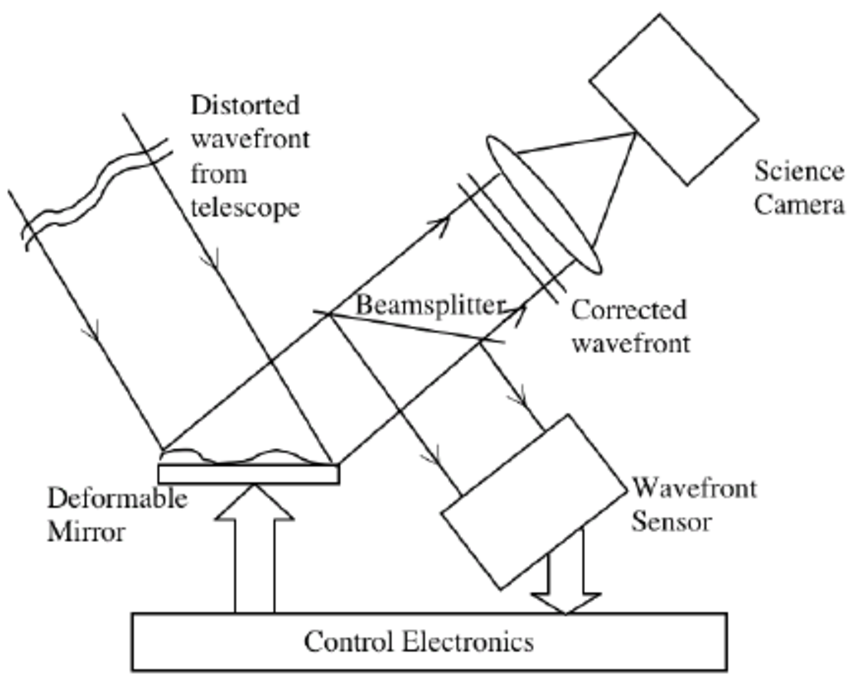
\includegraphics[width=0.5\linewidth,height=\textheight,keepaspectratio]{geometrical-optics/img/adaptive_optics.png}

}

\caption{Principle of adaptive optics. The image of a star is distorted
by the atmosphere. The distortion is measured with the help of a laser
beam and corrected with the help of a deformable mirror.}

\end{figure}%

\subsection{Space-Based Telescopes}\label{space-based-telescopes}

Placing telescopes in space eliminates atmospheric interference
completely. The Hubble Space Telescope revolutionized astronomy with its
crystal-clear views of the universe.

\begin{figure}[H]

{\centering 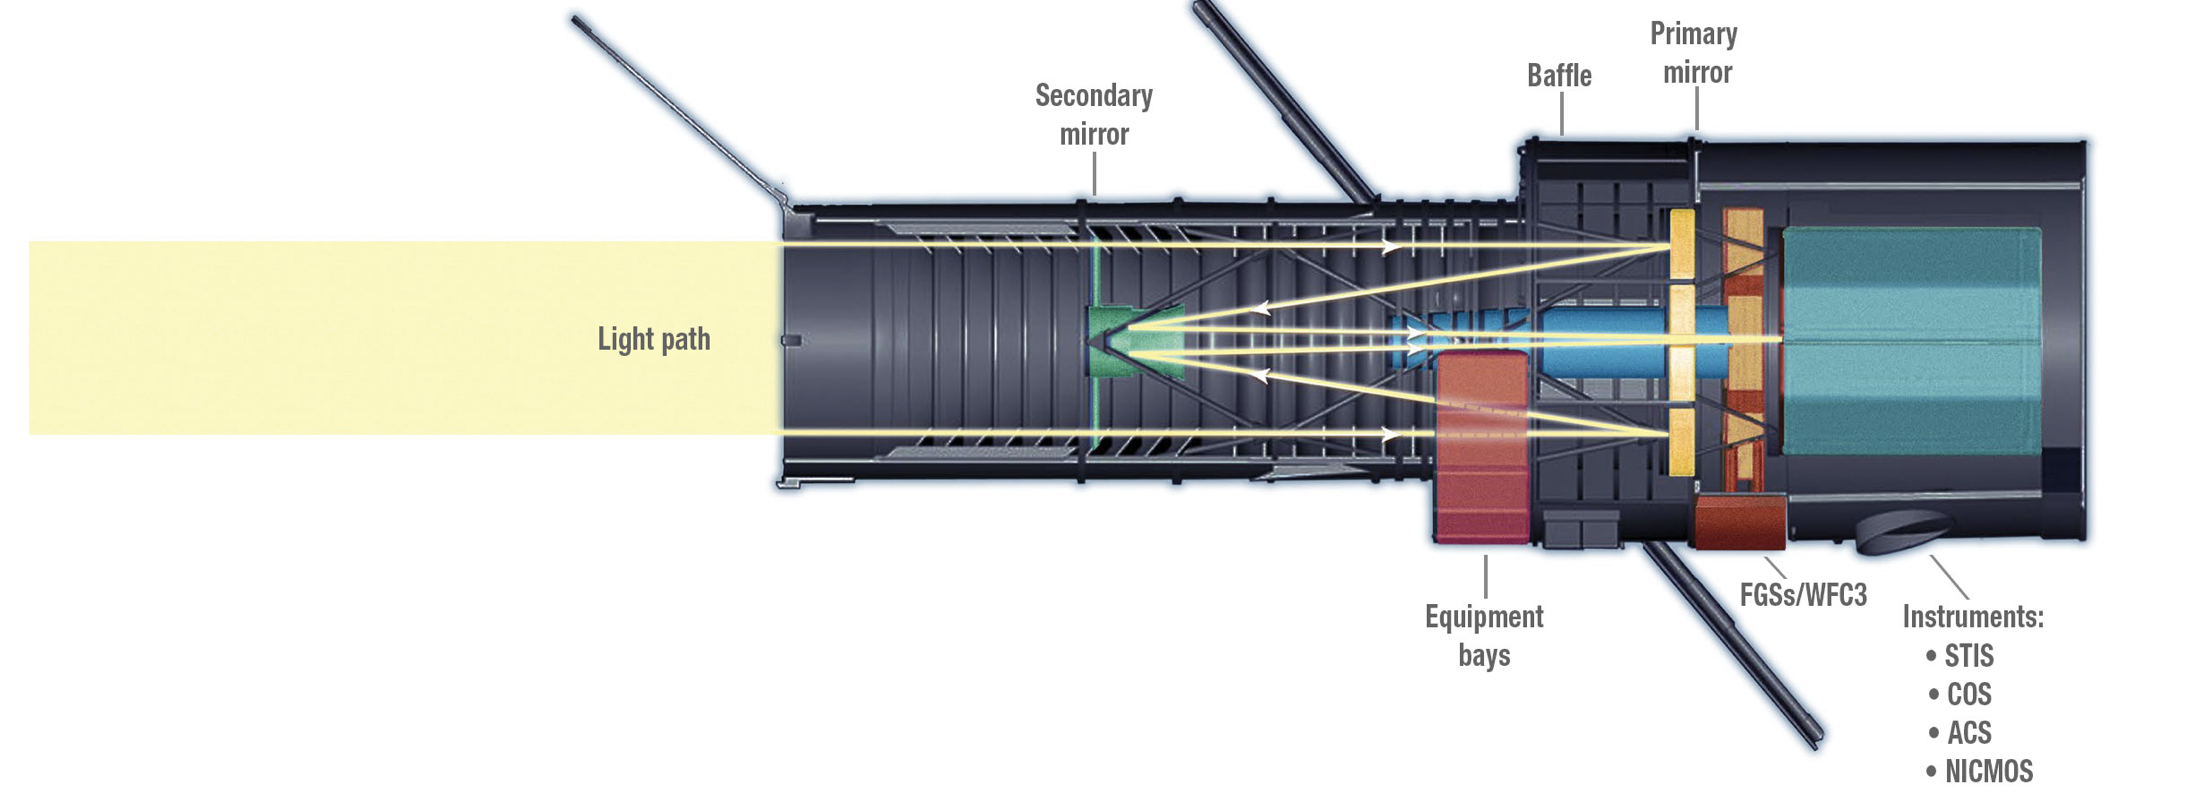
\includegraphics[width=1\linewidth,height=\textheight,keepaspectratio]{geometrical-optics/img/hubble.png}

}

\caption{Light path in the Hubble space telescope.}

\end{figure}%

Its successor, the James Webb Space Telescope (launched in 2021),
operates in the infrared spectrum and can peer even further into space
and time. Being above the atmosphere not only provides clearer images
but also allows these telescopes to observe wavelengths that are
normally blocked by Earth's atmosphere, particularly in the infrared and
ultraviolet regions.

\subsection{Beyond Optical Telescopes}\label{beyond-optical-telescopes}

While the principles discussed above apply primarily to optical
telescopes that observe visible light, it is worth noting that
telescopes exist for other regions of the electromagnetic spectrum as
well. Radio telescopes, for example, use large parabolic dishes to
collect and focus radio waves from cosmic sources. These instruments
operate on the same basic ray optics principles as reflecting optical
telescopes, with the dish acting as the primary mirror. Radio telescope
arrays, such as the Very Large Array (VLA) or the Atacama Large
Millimeter Array (ALMA), combine signals from multiple dishes using
interferometry techniques to achieve extremely high effective apertures.
Unlike optical telescopes, radio telescopes can observe through clouds
and during daytime, and they reveal phenomena invisible to optical
instruments, such as the radio emission from pulsars and the cosmic
microwave background radiation.

\chapter{Imaging Errors}\label{imaging-errors}

During our derivation of the imaging equation for lenses and the
lens-maker equation we have been working under the paraxial
approximation. This approximation stated, that all rays are close to the
optical axis and therefore make only small angles with the surface
normals of the curved surfaces of lenses (but also mirrors). If we
violate this approximation, i.e.~if we use rays, which are incident for
from the optical axis or strongly inclined, then we end up with
reflections and refraction which do not obey the imaging equation. In
addition we have seen that light propagation for different colors is
subject to different refractive indices (remember the prism). Thus we
will induce aberrations, related to color. According to Seidel,
aberration are classified the following way

\begin{itemize}
\tightlist
\item
  chromatic aberration
\item
  spherical aberration
\item
  coma
\item
  astigmatism
\item
  field curvature
\item
  field distortion
\end{itemize}

\section{Chromatic Aberration}\label{chromatic-aberration}

Chromatic Aberration are based on the fact that light of different color
has a different speed of propgation and thus also a different refractive
index. We experienced that also for the prism, where it was useful to
create a spectrograph. Here it is causing colored edges in you image,
which you do not want.

As the refractive index for shorter wavelength is typically higher, we
expect that the blue color has a shorter focal distance than the red
color.

\begin{figure}

\begin{minipage}{\linewidth}

\centering{

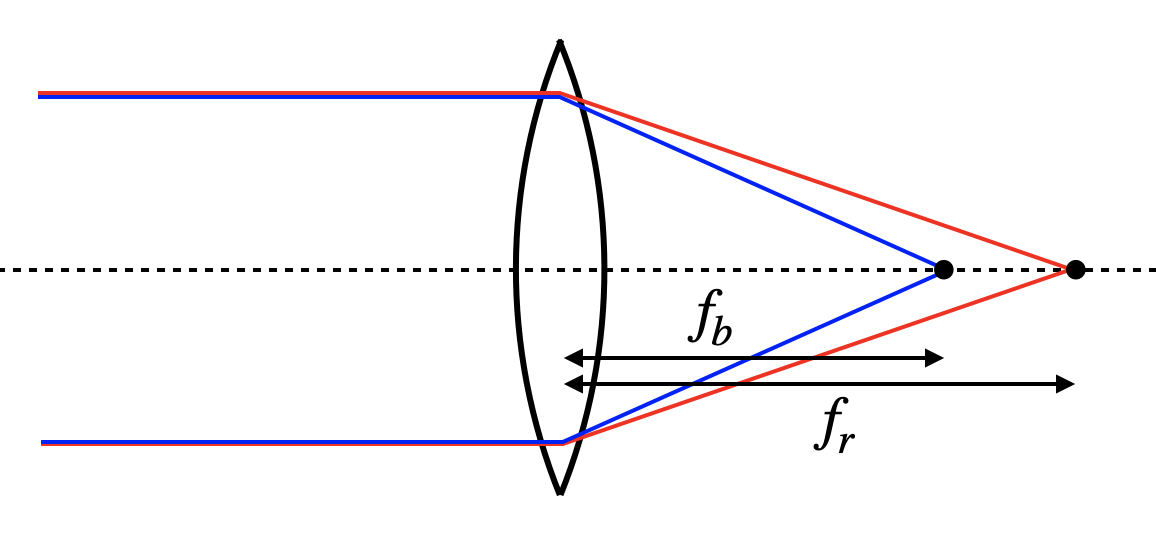
\includegraphics[width=0.6\linewidth,height=\textheight,keepaspectratio]{geometrical-optics/img/chromatic.png}

}

\subcaption{\label{fig-sketch}Sketch}

\end{minipage}%
\newline
\begin{minipage}{0.50\linewidth}

\centering{

\pandocbounded{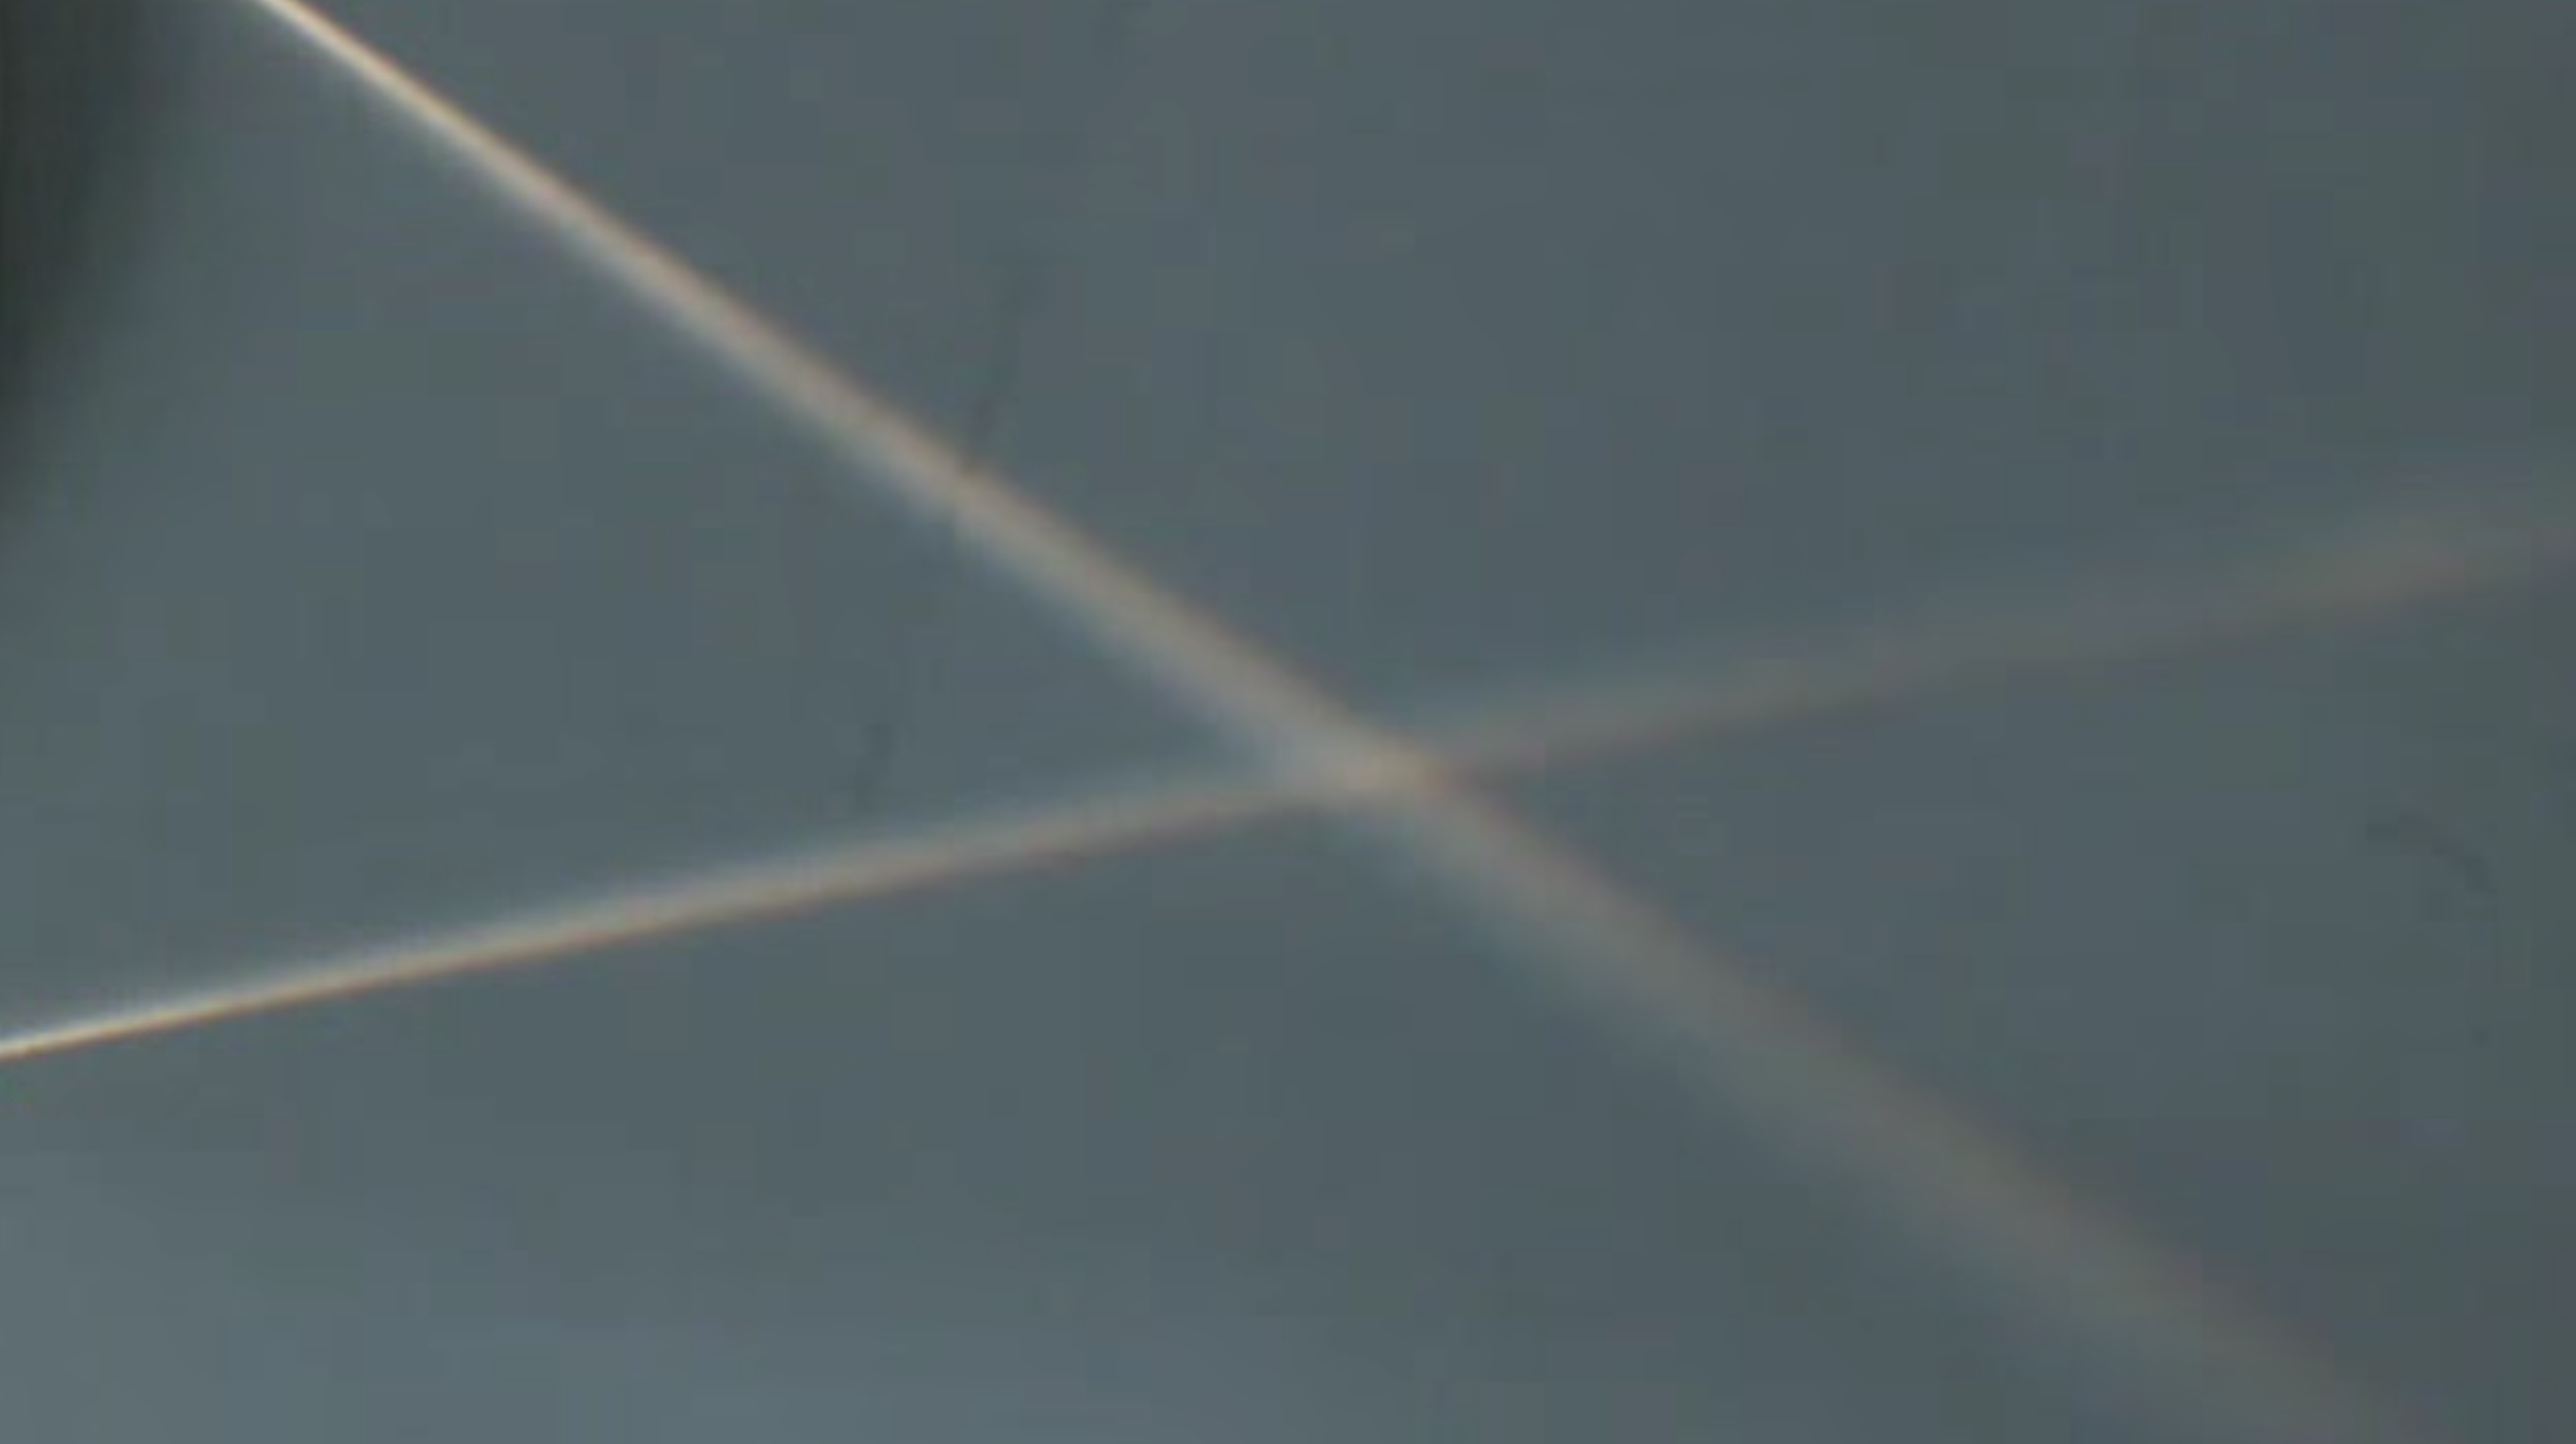
\includegraphics[keepaspectratio]{geometrical-optics/img/chromatic_exp.png}}

}

\subcaption{\label{fig-lecture}Lecture}

\end{minipage}%
%
\begin{minipage}{0.50\linewidth}

\centering{

\pandocbounded{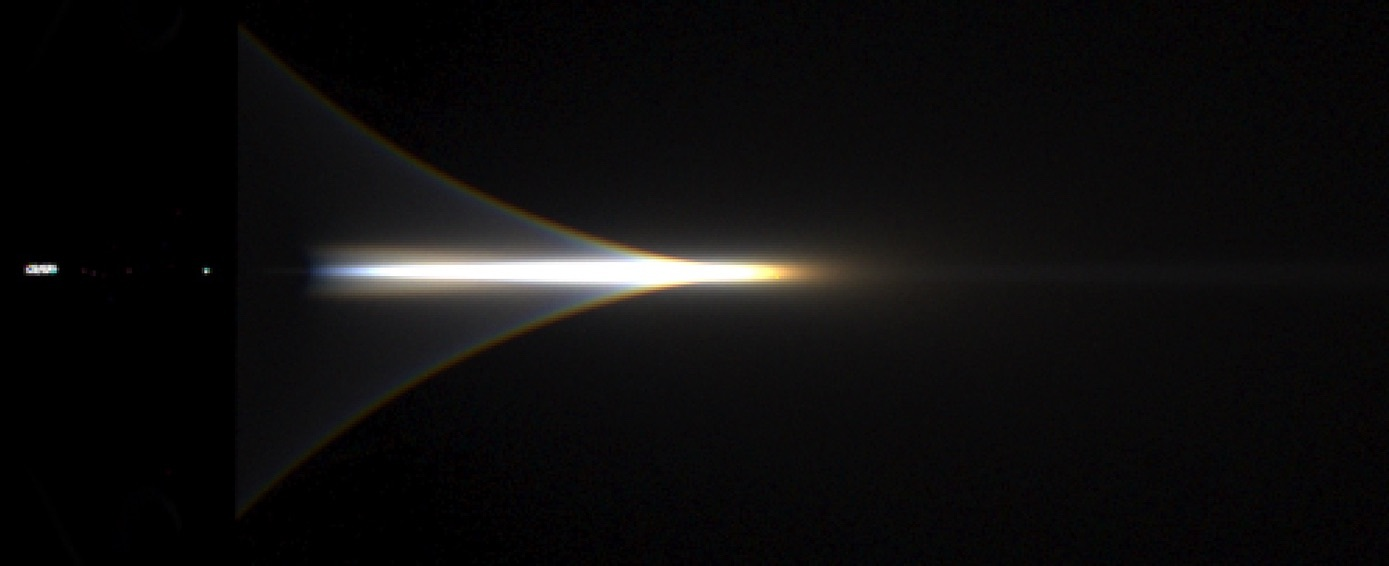
\includegraphics[keepaspectratio]{geometrical-optics/img/chromatic_rend.jpeg}}

}

\subcaption{\label{fig-rendered}Rendered}

\end{minipage}%

\caption{\label{fig-chromatic-aberration}Chromatic aberration. Left:
Sketch of the chromatic aberration, focusing red light less strong than
blue. Middle: Image from the lecture. Right: Rendered image using the
refractive index for BK7 glass.}

\end{figure}%

Here is a plot for the variation of the focal distance of a lens with a
radius of curvature of 100 mm as a function of the wavelength for three
different glasses.

\begin{figure}[H]

{\centering \pandocbounded{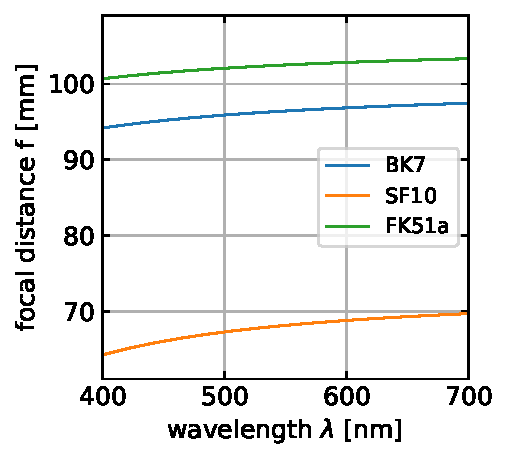
\includegraphics[keepaspectratio]{geometrical-optics/Imaging Errors_files/figure-pdf/cell-3-output-1.pdf}}

}

\caption{Focal distance of a Bk7, SF10 and FK51a lens with a radius of
curvature of 100 mm as a function of the wavelength.}

\end{figure}%

Such a chromatic aberrations may be corrected by using a system of two
lenses as shown below.

\begin{figure}

\centering{

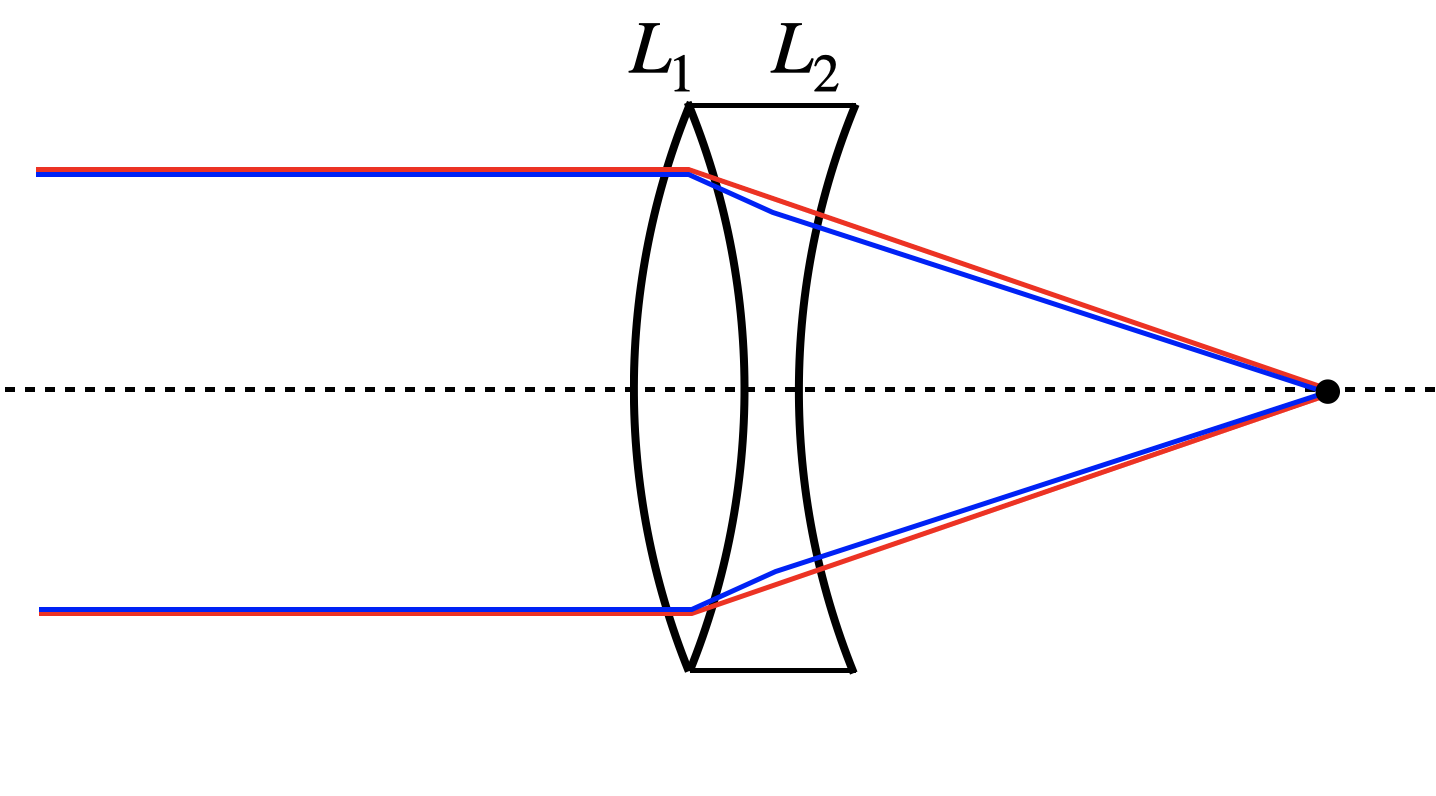
\includegraphics[width=0.6\linewidth,height=\textheight,keepaspectratio]{geometrical-optics/img/achromat.png}

}

\caption{\label{fig-achromat}Correction of chromatic aberration by a
lens doublet with a convex and a a concave lens.}

\end{figure}%

Chromatic aberration can be corrected by using an achromatic lens.
Achromatic lenses are typically constructed by combining two lenses with
different optical properties: a biconvex lens made of crown glass (lower
dispersion) bonded to a biconcave lens made of flint glass (higher
dispersion). This combination allows for the correction of chromatic
aberration. Each lens \(i\) has a focal length according to the
lensmaker equation:

\[
\frac{1}{f_i}=(n_i-1)\rho_i
\]

where \(\rho_i\) is given by:

\[
\rho_i=\frac{(R_{i2}-R_{i1})}{R_{i1}R_{i2}}
\]

For a system of two lenses in contact, the total refractive power is:

\[
\frac{1}{f}=(n_1-1)\rho_1+(n_2-1)\rho_2
\]

For color correction, we require equal focusing of red and blue light:

\[
(n_{1r}-1)\rho_1+(n_{2r}-1)\rho_2=(n_{1b}-1)\rho_1+(n_{2b}-1)\rho_2
\]

This transforms to:

\[
\frac{\rho_1}{\rho_2}=-\frac{n_{2b}-n_{2r}}{n_{1b}-n_{1r}}
\]

For the specific geometry shown in the achromat figure where:

\begin{itemize}
\tightlist
\item
  \(R_{12}=R_{21}\) (common radius at contact surface)
\item
  \(R_{11}=R_1=-R_{12}=-R_{21}\)
\item
  \(R_{22}=R_2\)
\end{itemize}

we can express \(\rho_1\) and \(\rho_2\) as:

\[
\rho_1=\frac{2}{R_1} \quad \text{and} \quad \rho_2=\frac{-1}{R_1}+\frac{1}{R_2}
\]

Substituting these into the color correction condition gives us the
relationship between \(R_1\) and \(R_2\) needed for an achromatic
doublet. Substituting the expressions for \(\rho_1\) and \(\rho_2\)
into:

\[
\frac{\rho_1}{\rho_2}=-\frac{n_{2b}-n_{2r}}{n_{1b}-n_{1r}}
\]

we get:

\[
\frac{2/R_1}{-1/R_1+1/R_2}=-\frac{n_{2b}-n_{2r}}{n_{1b}-n_{1r}}
\]

Let's define the dispersion ratios (typically called V-numbers or Abbe
numbers): \[
V_1=\frac{n_{1r}-1}{n_{1b}-n_{1r}} \quad \text{and} \quad V_2=\frac{n_{2r}-1}{n_{2b}-n_{2r}}
\]

Then, after some algebra, the relationship between \(R_1\) and \(R_2\)
becomes:

\[
\frac{R_2}{R_1}=1+2\frac{V_2(n_{1r}-1)}{V_1(n_{2r}-1)}
\]

This equation determines the ratio of radii needed to achieve an
achromatic doublet for the chosen glass materials.

\begin{tcolorbox}[enhanced jigsaw, breakable, toptitle=1mm, bottomrule=.15mm, colbacktitle=quarto-callout-note-color!10!white, title=\textcolor{quarto-callout-note-color}{\faInfo}\hspace{0.5em}{Chromatic Aberration}, arc=.35mm, rightrule=.15mm, bottomtitle=1mm, opacityback=0, toprule=.15mm, coltitle=black, leftrule=.75mm, opacitybacktitle=0.6, colback=white, left=2mm, titlerule=0mm, colframe=quarto-callout-note-color-frame]

An optical aberration caused by the wavelength-dependent refractive
index of materials, resulting in different colors focusing at different
distances from the lens, typically with blue light focusing closer to
the lens than red light.

\end{tcolorbox}

\section{Spherical Aberration}\label{spherical-aberration}

The spherical abberation arises due to the fact that we have always
considered a simplification of the angluar functions to their first
order Taylor series expansion. If the angles of incidence on the
spherical surfaces get to large, we cannot do that anymore and need to
consider higher order corrections.

The result is that parallel rays which are far from the optical axis are
not imaged into the same focal point as the paraxial rays, but to points
closer to the lens. You might have all seen such effect also in the case
of your empty coffee cup, when the sunlight enters and causes a
so-called caustics. This pattern, you observe there is also the result
of a soherical aberration. The image below shows the spherical
aberration of a lens.

\begin{figure}

\begin{minipage}{0.50\linewidth}

\centering{

\pandocbounded{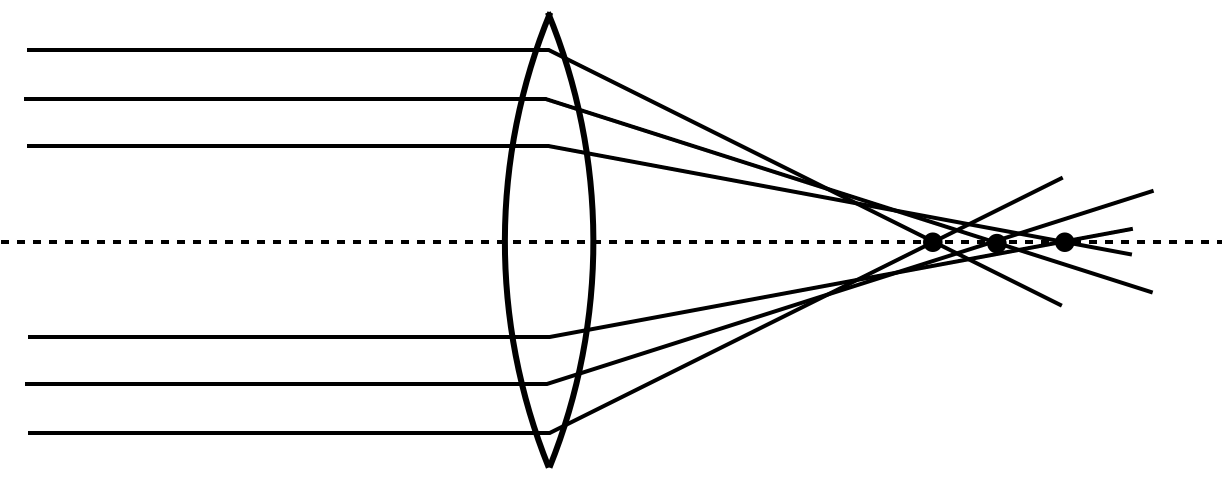
\includegraphics[keepaspectratio]{geometrical-optics/img/spherical.png}}

}

\subcaption{\label{fig-sketch-spherical}Sketch}

\end{minipage}%
%
\begin{minipage}{0.50\linewidth}

\centering{

\pandocbounded{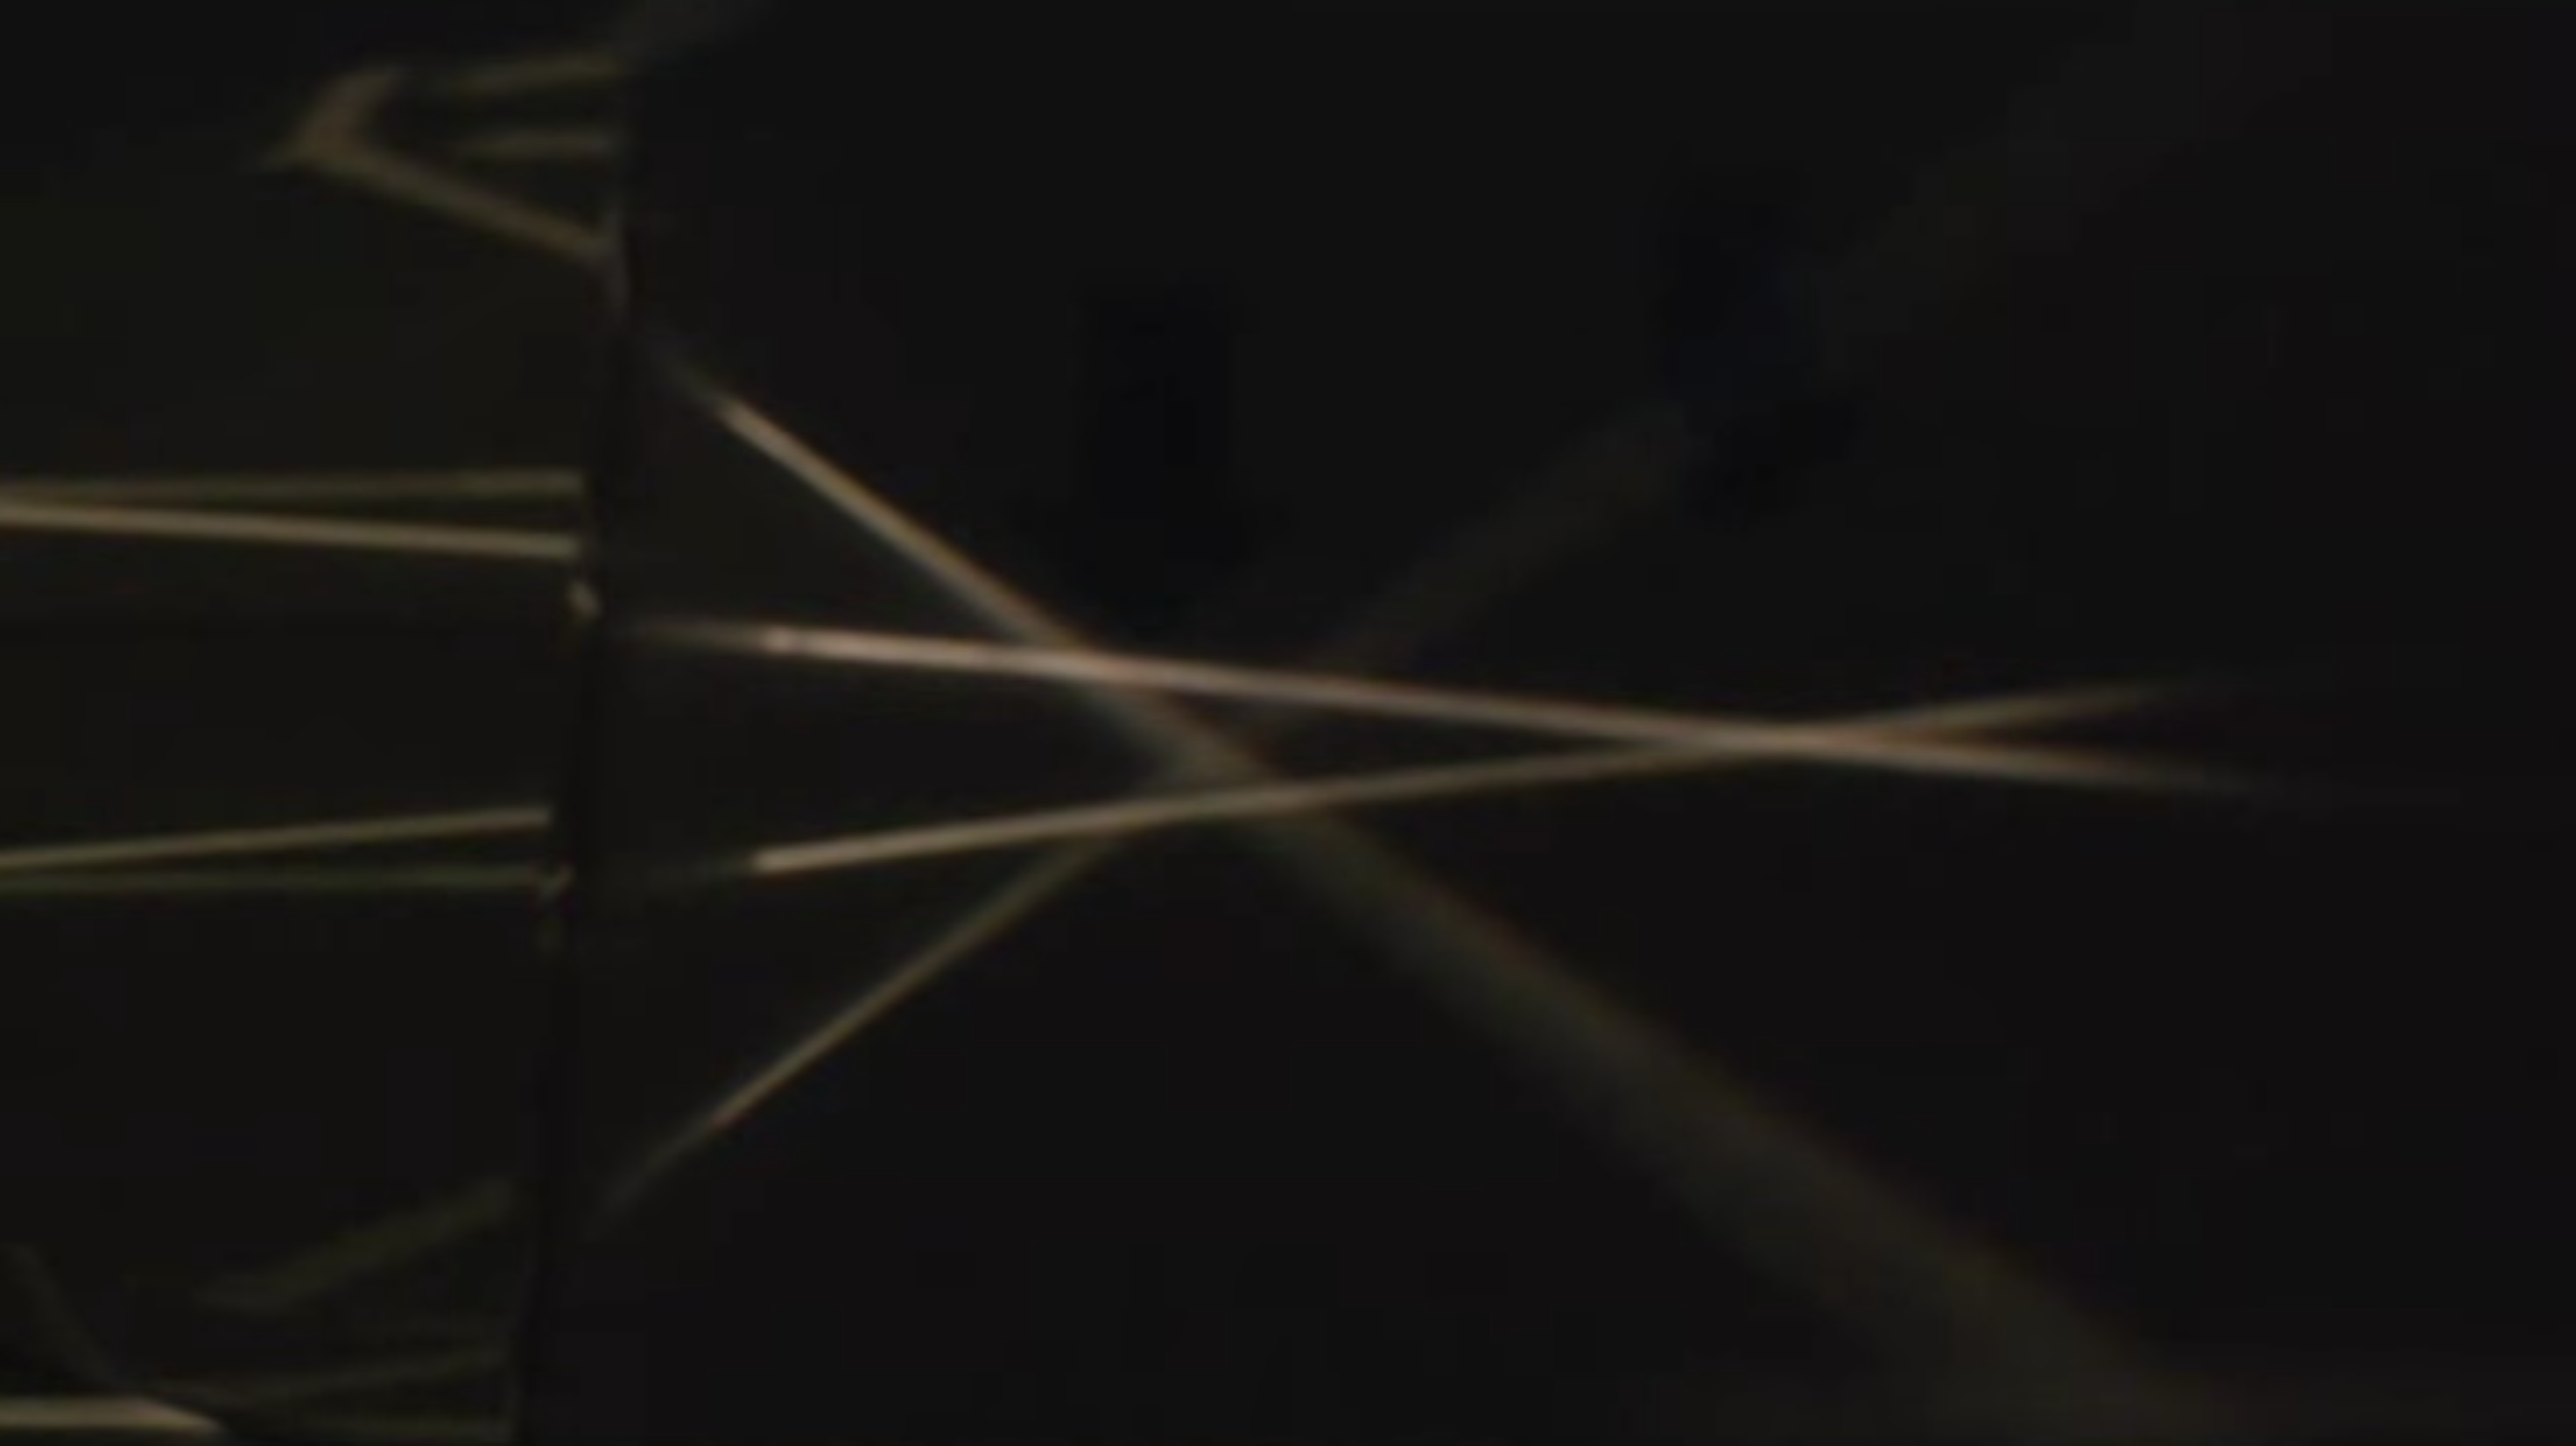
\includegraphics[keepaspectratio]{geometrical-optics/img/spherical_exp.png}}

}

\subcaption{\label{fig-exp-spherical}Experimental}

\end{minipage}%

\caption{\label{fig-spherical}Spherical aberration. Left: Schematic
illustration showing how parallel rays at different distances from the
optical axis focus at different points. Right: Experimental
demonstration from the lecture.}

\end{figure}%

To be a bit more qauntitative, we would like to reconsider the
refraction at a single spherical surface as depicted in the image below.

\begin{figure}

\centering{

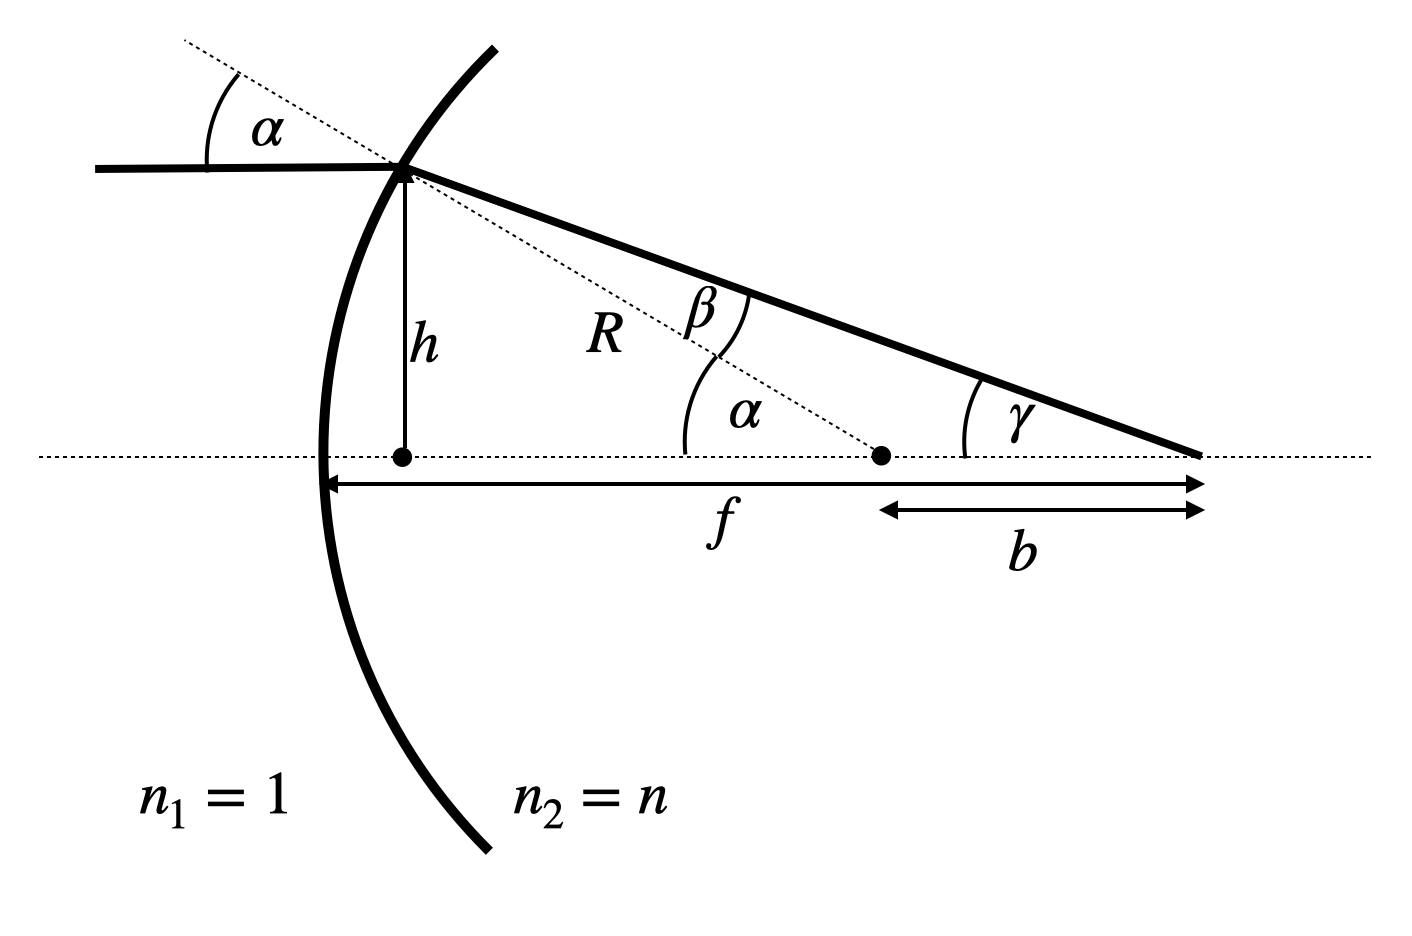
\includegraphics[width=0.6\linewidth,height=\textheight,keepaspectratio]{geometrical-optics/img/spherical_theo.png}

}

\caption{\label{fig-spherical-theo}Spherical aberration: Theoretical ray
tracing showing the focal point variation with incident ray height.}

\end{figure}%

For spherical surfaces, we can derive a more accurate expression for the
focal length using the following relations:
\[\sin(\beta)=\frac{\sin(\alpha)}{n}, \quad \sin(\alpha)=\frac{h}{R}, \quad \alpha=\beta+\gamma\]

Using these relations, we obtain \(f=R+b\) and
\(b=R\sin(\beta)/\sin(\gamma)\), which can be transformed into:

\[
f=R\left [ 1+ \frac{1}{n\cos(\beta)-\cos(\alpha)}\right ]
\]

By replacing the cosines with their corresponding expressions, we get:

\[
f=R\left [ 1+ \frac{1}{n\sqrt{1-\frac{h^2}{n^2 R^2}}-\sqrt{1-\frac{h^2}{R^2}}}\right ]
\]

Expanding the square roots leads to:

\[
f=R\left [ \frac{n}{n-1}- \frac{h^2}{2n(n-1)R^2} \right]
\]

This result reveals that the focal length depends on the height \(h\) at
which the ray is incident on the spherical surface, similar to the case
of concave mirrors. The second term in the square brackets represents
this height-dependent contribution, which reduces the focal length when
\(h\neq 0\).

From these relations, we can derive an imaging equation for a single
spherical surface:

\[
\frac{1}{a}+\frac{n}{b}=\frac{n-1}{R}+h^2\left [ \frac{1}{2a}\left ( \frac{1}{a}+\frac{1}{R}\right )^2 +\frac{n}{2b}\left ( \frac{1}{R}-\frac{1}{b}\right )^2\right]
\]

This complex equation for a single surface demonstrates that the image
is no longer formed on a plane; instead, its location depends on both
\(R\) and \(h\). This height dependence for a single surface manifests
in various image distortions, including field curvature.

\begin{tcolorbox}[enhanced jigsaw, breakable, toptitle=1mm, bottomrule=.15mm, colbacktitle=quarto-callout-note-color!10!white, title=\textcolor{quarto-callout-note-color}{\faInfo}\hspace{0.5em}{Spherical Aberration}, arc=.35mm, rightrule=.15mm, bottomtitle=1mm, opacityback=0, toprule=.15mm, coltitle=black, leftrule=.75mm, opacitybacktitle=0.6, colback=white, left=2mm, titlerule=0mm, colframe=quarto-callout-note-color-frame]

An optical aberration where rays passing through a lens at different
distances from the optical axis focus at different points along the
axis, with rays through the outer regions of the lens focusing closer to
the lens than rays passing near the center.

\end{tcolorbox}

\section{Field Curvature}\label{field-curvature}

The field curvature is related to our calculations of the spherical
abberation. We have seen there, that the focal distance depends on the
height \(h\) of the rays over the optical axis. This means also means
that the image plane is actually not anymore a plane but a curved
surface as shown below. The rays incident from point \(A_0\) and \(A_1\)
do not meet in the same plane. This plane is even different for
meridional and saggital rays. This typically results in the fact, that
you may have the center of the image in focus, but not the edges or vice
versa.

\begin{figure}

\begin{minipage}{0.50\linewidth}

\centering{

\pandocbounded{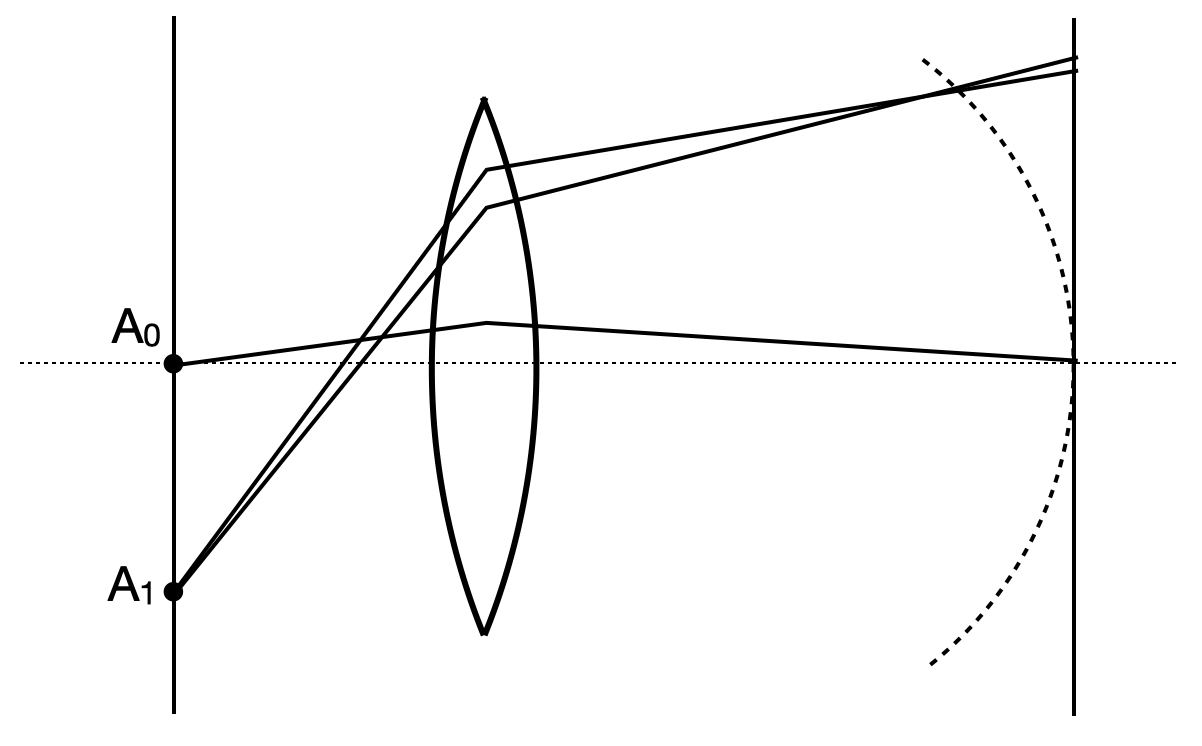
\includegraphics[keepaspectratio]{geometrical-optics/img/field_curv.png}}

}

\subcaption{\label{fig-fieldcurv-sketch}Sketch}

\end{minipage}%
%
\begin{minipage}{0.50\linewidth}

\centering{

\pandocbounded{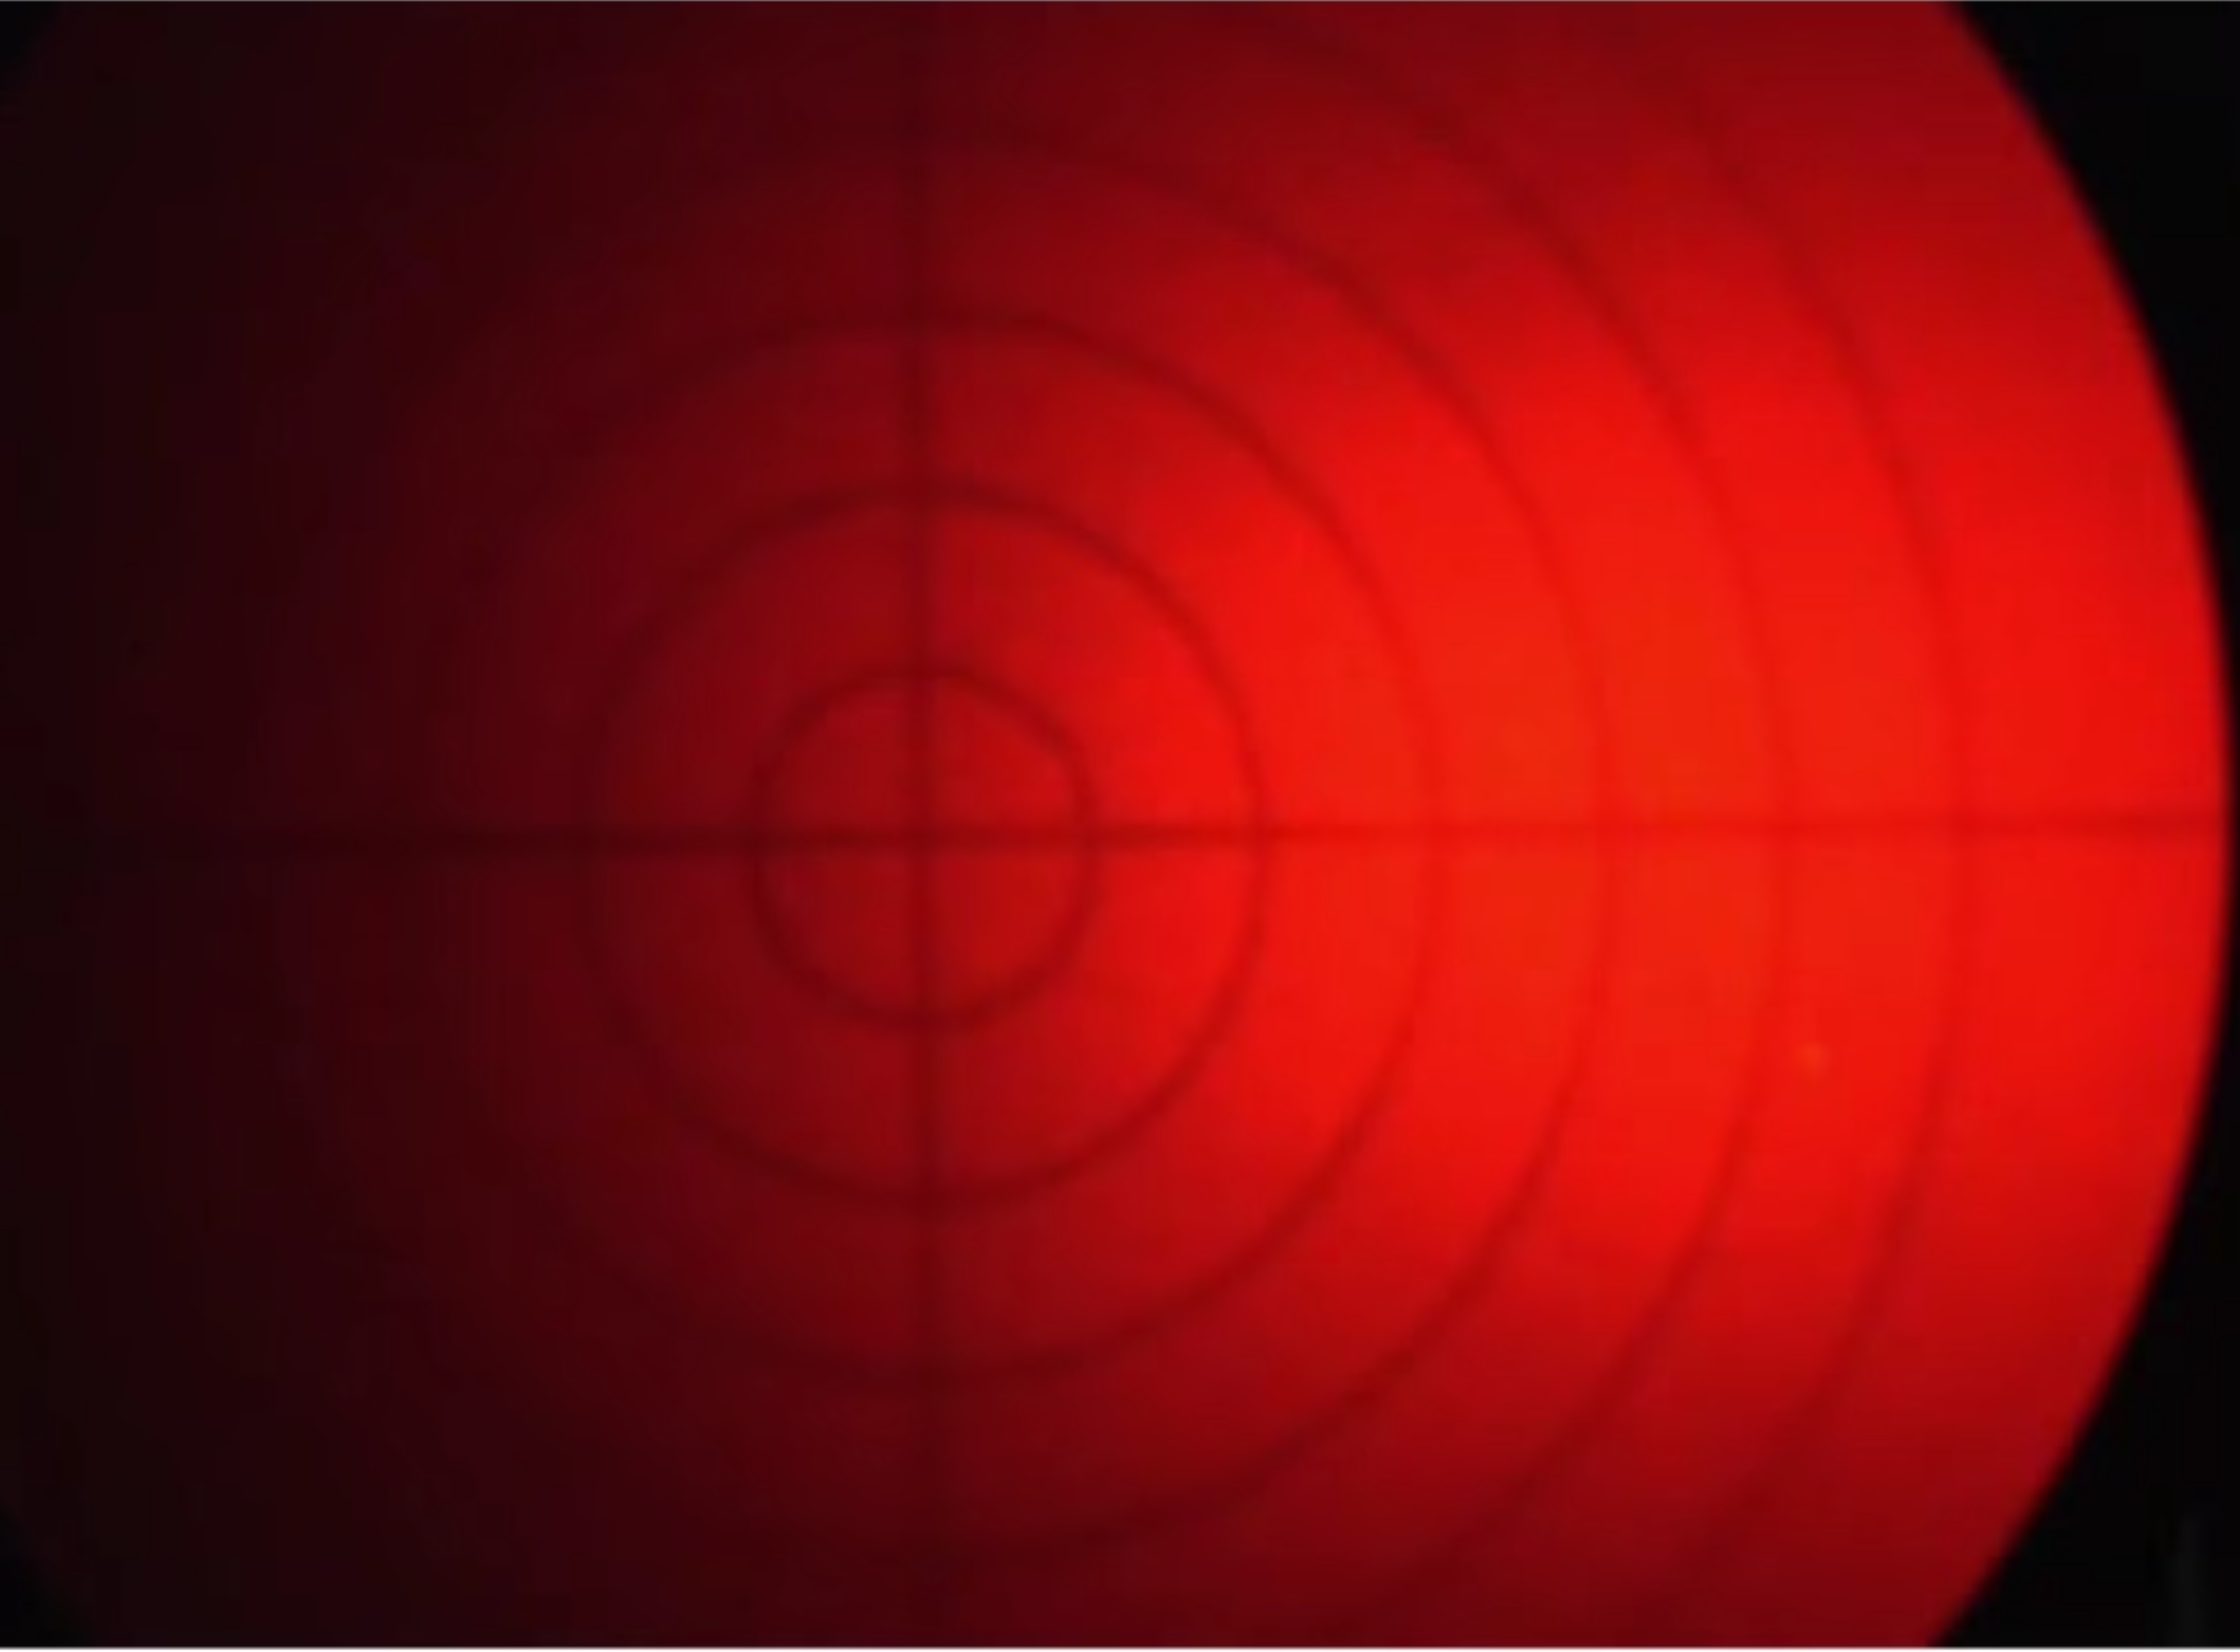
\includegraphics[keepaspectratio]{geometrical-optics/img/fieldcurvature_exp.png}}

}

\subcaption{\label{fig-fieldcurv-exp}Experimental}

\end{minipage}%

\caption{\label{fig-field-curvature}Field curvature in optical systems.
Left: Schematic diagram showing how a flat object plane is imaged onto a
curved image surface (Petzval surface) rather than a flat image plane.
This causes different regions of the image to focus at different
distances from the lens. Right: Experimental demonstration showing how
either the center or the edges of the image can be in focus, but not
simultaneously, when using a flat detector. This aberration is
particularly noticeable in wide-field imaging systems with simple
lenses.}

\end{figure}%

\begin{tcolorbox}[enhanced jigsaw, breakable, toptitle=1mm, bottomrule=.15mm, colbacktitle=quarto-callout-note-color!10!white, title=\textcolor{quarto-callout-note-color}{\faInfo}\hspace{0.5em}{Field Curvature}, arc=.35mm, rightrule=.15mm, bottomtitle=1mm, opacityback=0, toprule=.15mm, coltitle=black, leftrule=.75mm, opacitybacktitle=0.6, colback=white, left=2mm, titlerule=0mm, colframe=quarto-callout-note-color-frame]

An optical aberration where the image of a flat object is formed on a
curved surface rather than a plane, causing the center and edges of the
image field to not be simultaneously in focus on a flat detector or
screen.

\end{tcolorbox}

\section{Coma}\label{coma}

While our previous discussion focused on rays parallel to the optical
axis at varying distances, significant aberrations also occur for rays
emanating from off-axis object points (both at finite and infinite
distances). One important example of such an aberration is ``coma.''

In the case of coma, rays entering the lens at different heights with an
angle to the optical axis do not converge to a single point in the image
plane. Instead, they create a characteristic comet-shaped intensity
distribution, where the light is asymmetrically distributed with a
bright head and a diffuse tail pointing radially outward from the
optical axis. This asymmetric distribution occurs because rays passing
through different zones of the lens experience different effective
magnifications, leading to the distinctive comet-like shape that gives
this aberration its name.

The severity of coma typically increases with the distance from the
optical axis and with larger apertures, making it particularly
problematic in wide-field imaging systems or when using large-aperture
optics.

\begin{figure}

\begin{minipage}{0.50\linewidth}

\centering{

\pandocbounded{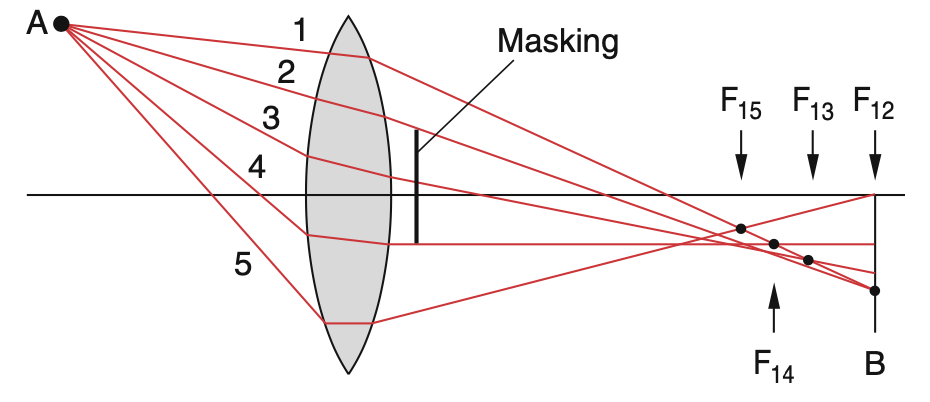
\includegraphics[keepaspectratio]{geometrical-optics/img/coma.png}}

}

\subcaption{\label{fig-coma-sketch}Sketch}

\end{minipage}%
%
\begin{minipage}{0.50\linewidth}

\centering{

\pandocbounded{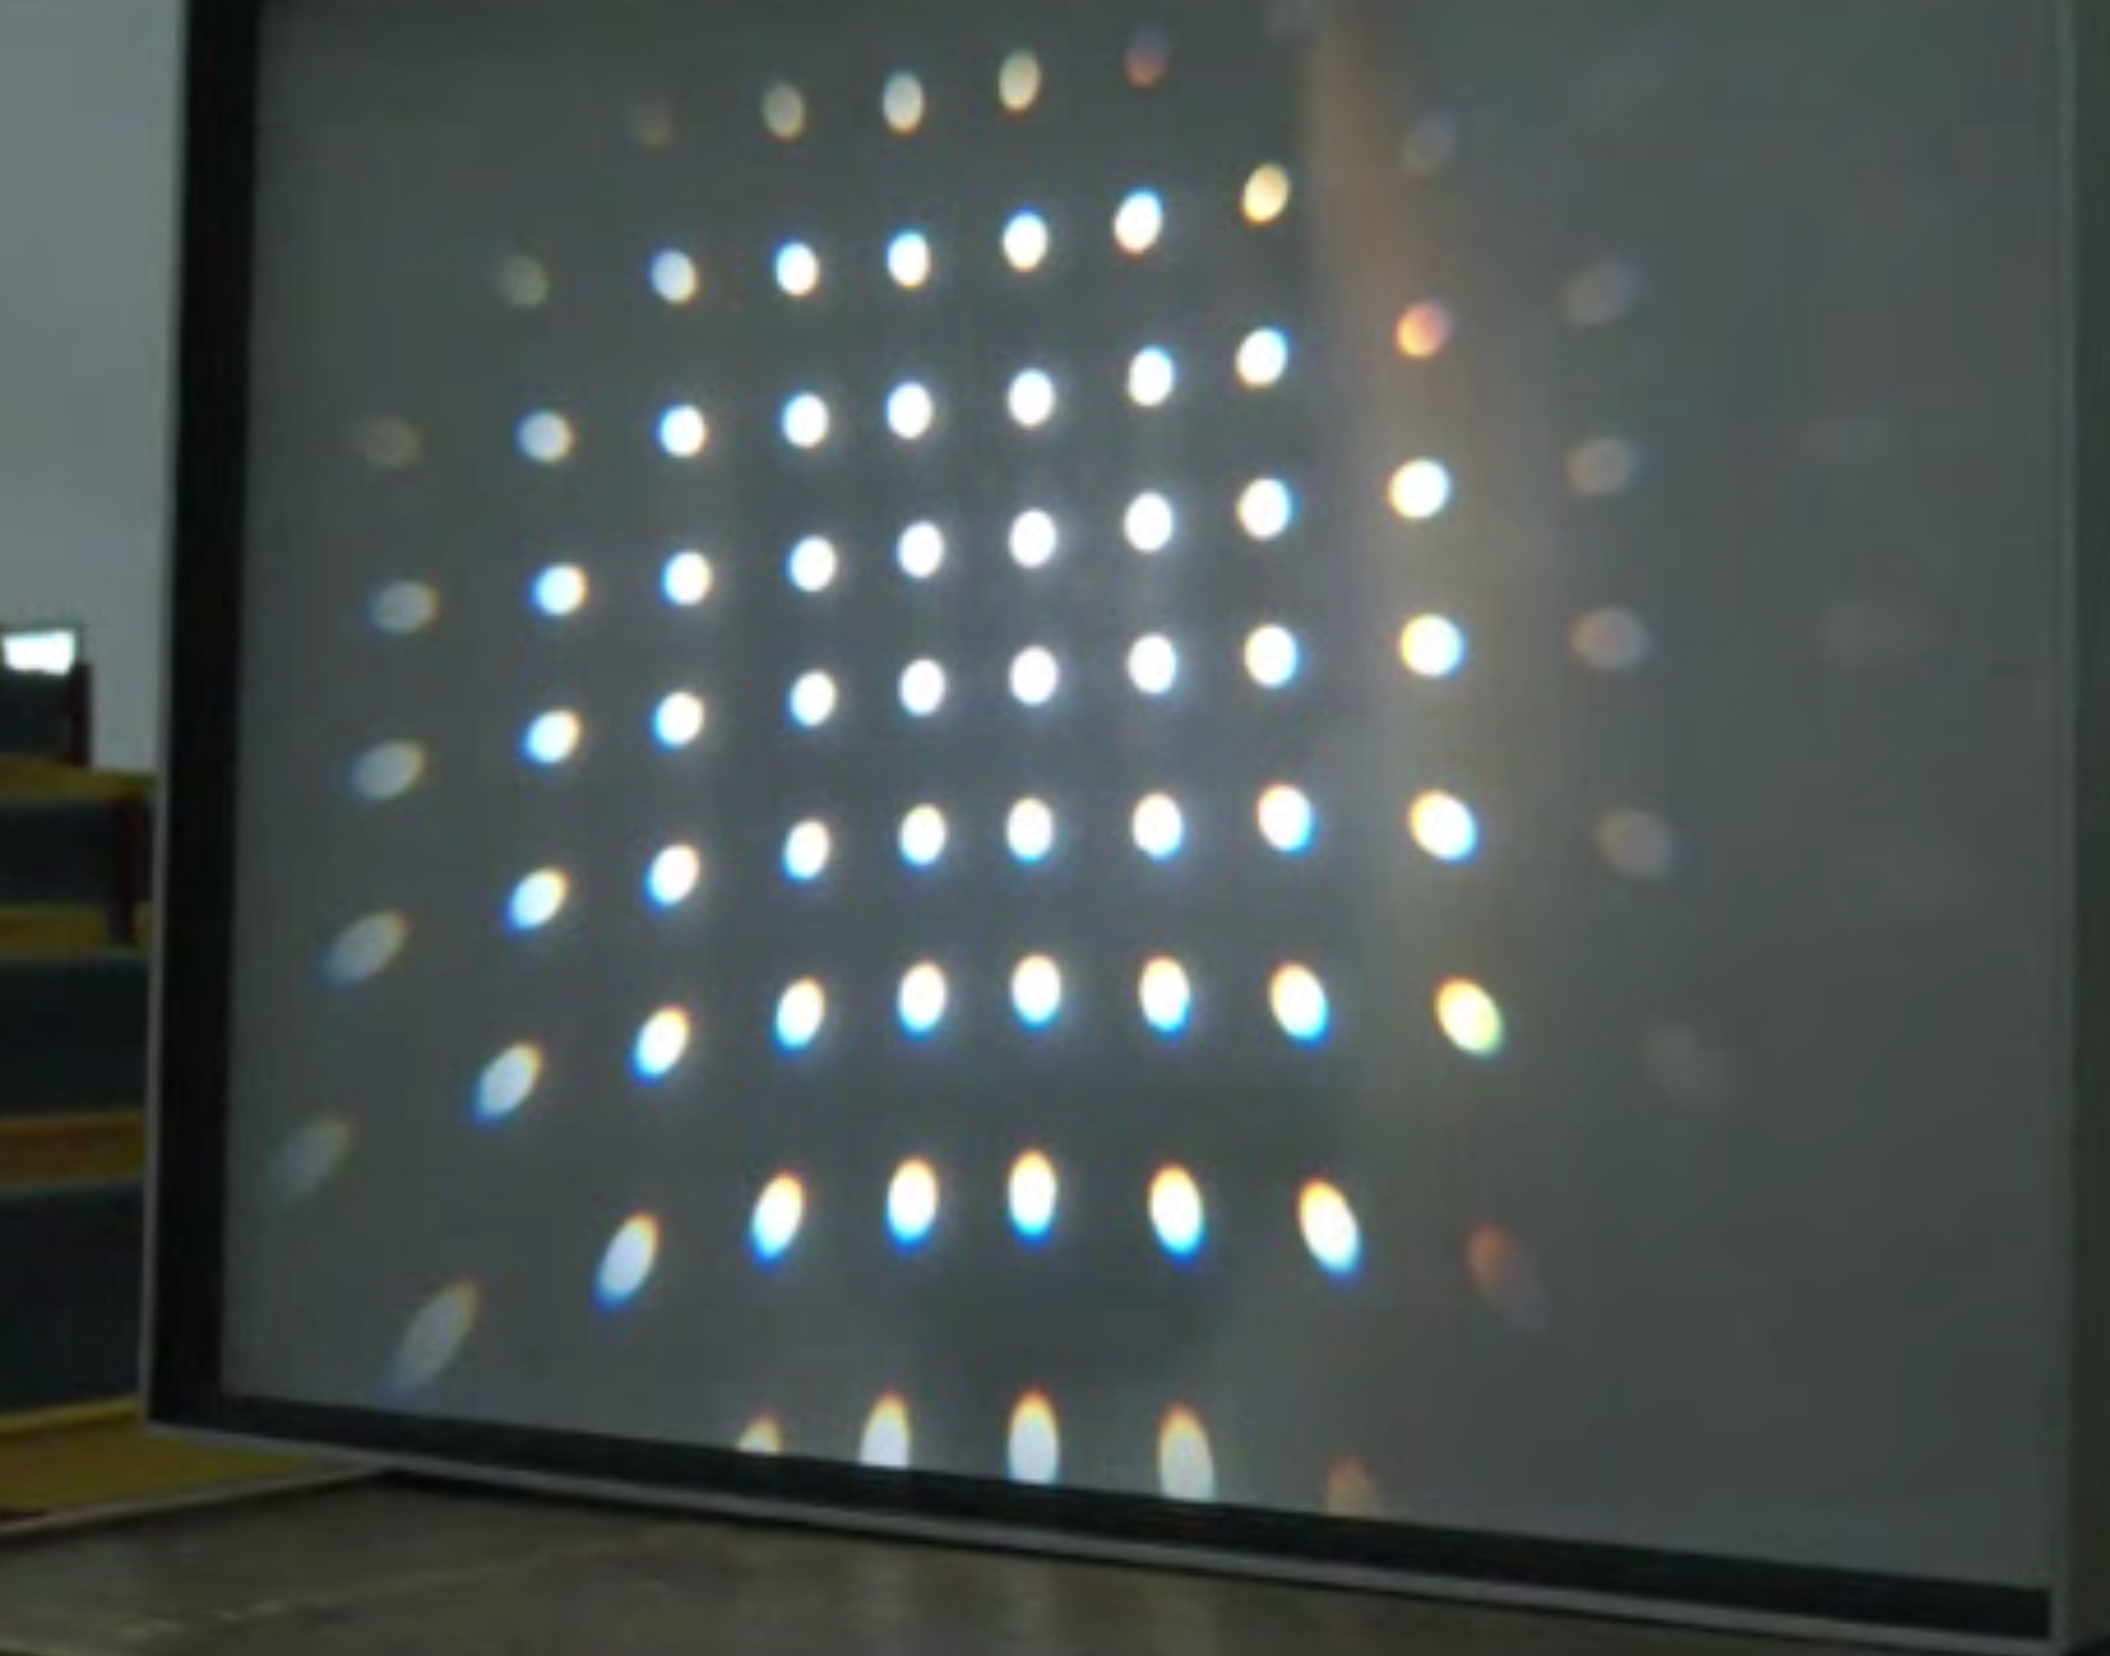
\includegraphics[keepaspectratio]{geometrical-optics/img/coma_exp.png}}

}

\subcaption{\label{fig-coma-exp}Experimental}

\end{minipage}%

\caption{\label{fig-coma}Coma aberration in optical systems. Left:
Schematic illustration showing how oblique rays entering the lens at
different heights focus at different positions in the image plane,
creating a characteristic comet-shaped blur (coma). The rays passing
through different zones of the lens have different effective focal
lengths and magnifications, resulting in the asymmetric image formation.
Right: Experimental demonstration from the lecture showing the
characteristic comet-like shape of the aberration, where the intensity
distribution is asymmetric around the central image point.}

\end{figure}%

\begin{tcolorbox}[enhanced jigsaw, breakable, toptitle=1mm, bottomrule=.15mm, colbacktitle=quarto-callout-note-color!10!white, title=\textcolor{quarto-callout-note-color}{\faInfo}\hspace{0.5em}{Coma}, arc=.35mm, rightrule=.15mm, bottomtitle=1mm, opacityback=0, toprule=.15mm, coltitle=black, leftrule=.75mm, opacitybacktitle=0.6, colback=white, left=2mm, titlerule=0mm, colframe=quarto-callout-note-color-frame]

An optical aberration where rays from an off-axis point source passing
through different zones of a lens focus at different positions in the
image plane, creating a characteristic comet-shaped intensity
distribution with a bright head and a diffuse tail pointing radially
outward.

\end{tcolorbox}

\section{Astigmatism}\label{astigmatism}

Astigmatism also occurs when imaging point sources located away from the
optical axis. To understand this effect, we can analyze the rays from
such a source by separating them into two categories:

\begin{enumerate}
\def\labelenumi{\arabic{enumi}.}
\tightlist
\item
  Rays in the vertical (meridional) plane
\item
  Rays in the perpendicular (sagittal) plane
\end{enumerate}

Analysis shows that meridional rays focus at a point closer to the lens
compared to sagittal rays. This difference in focal positions creates a
characteristic pattern in the image: when moving a screen through the
focal region, the image of a point source transforms from a horizontal
ellipse, through a circular point (at the circle of least confusion), to
a vertical ellipse. This variation in image shape occurs because the
focal surfaces for the meridional and sagittal rays are curved
differently and intersect only at points along the optical axis.

The distance between these two focal surfaces increases with the
distance from the optical axis, making astigmatism particularly
noticeable for off-axis object points. This aberration is especially
significant in systems where the object plane is not perpendicular to
the optical axis or when using simple spherical lenses for wide-field
imaging.

For an extended image as shown below, this results in the sperate
focusing of vertical (left) and horizontal lines (right) in the image.

\begin{figure}

\begin{minipage}{\linewidth}

\centering{

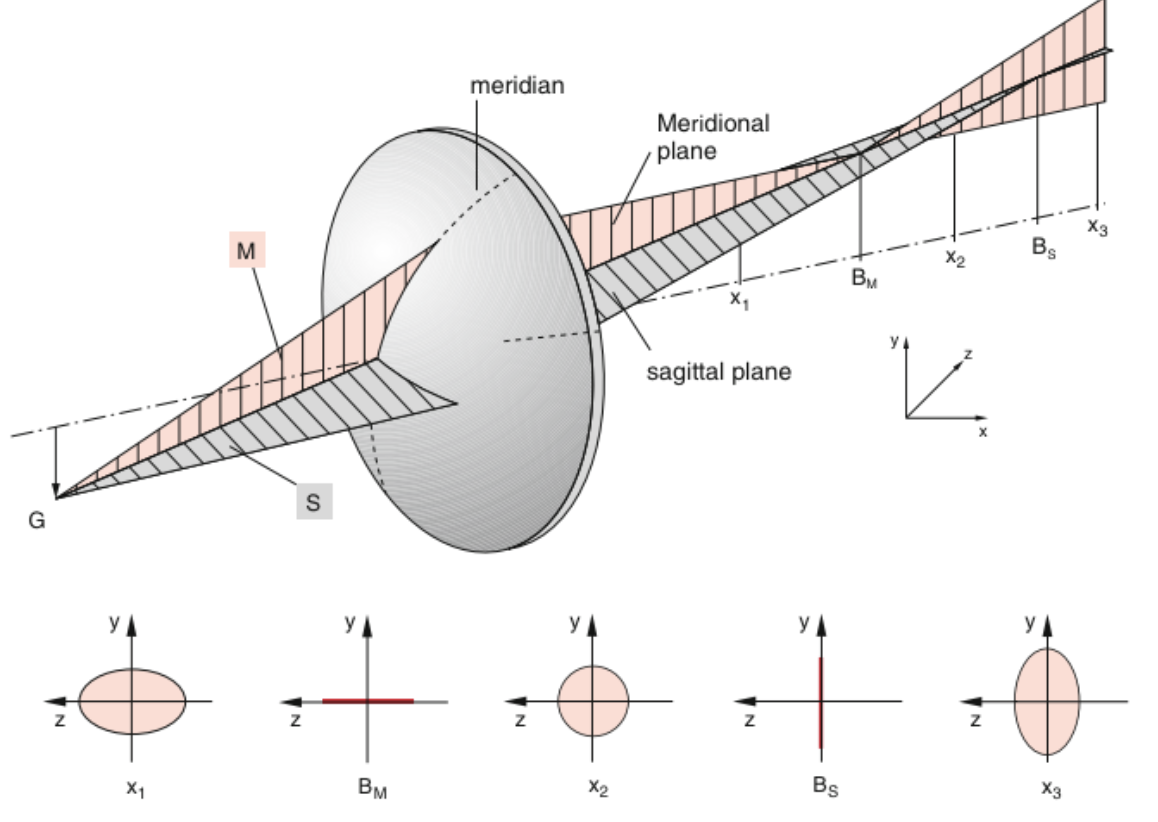
\includegraphics[width=0.6\linewidth,height=\textheight,keepaspectratio]{geometrical-optics/img/astigmatism.png}

}

\subcaption{\label{fig-astig-sketch}Sketch}

\end{minipage}%
\newline
\begin{minipage}{0.50\linewidth}

\centering{

\pandocbounded{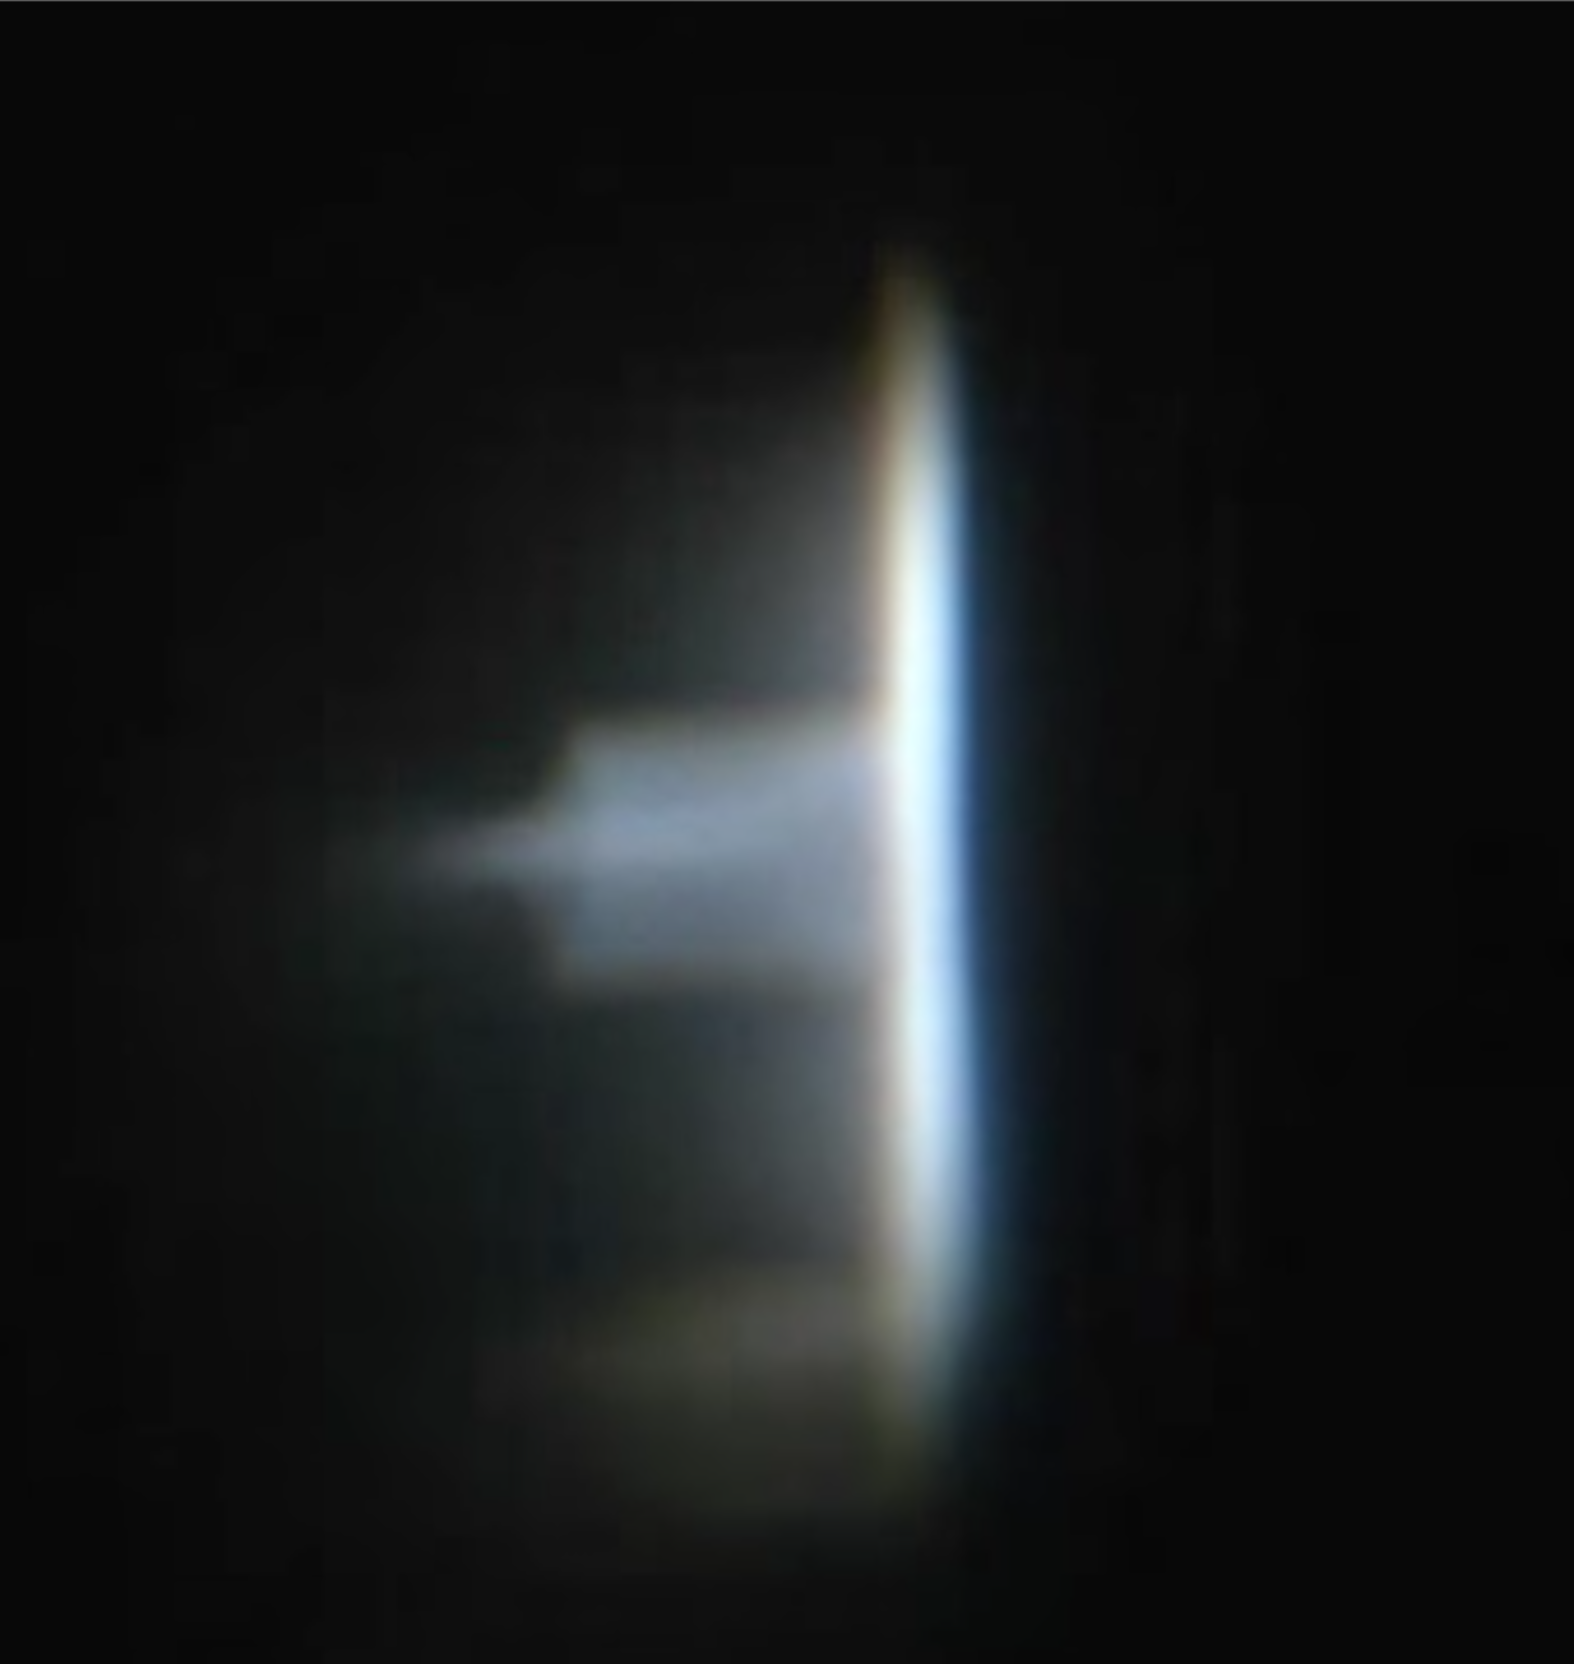
\includegraphics[keepaspectratio]{geometrical-optics/img/astigvert_exp.png}}

}

\subcaption{\label{fig-astig-vert}Vertical Focus}

\end{minipage}%
%
\begin{minipage}{0.50\linewidth}

\centering{

\pandocbounded{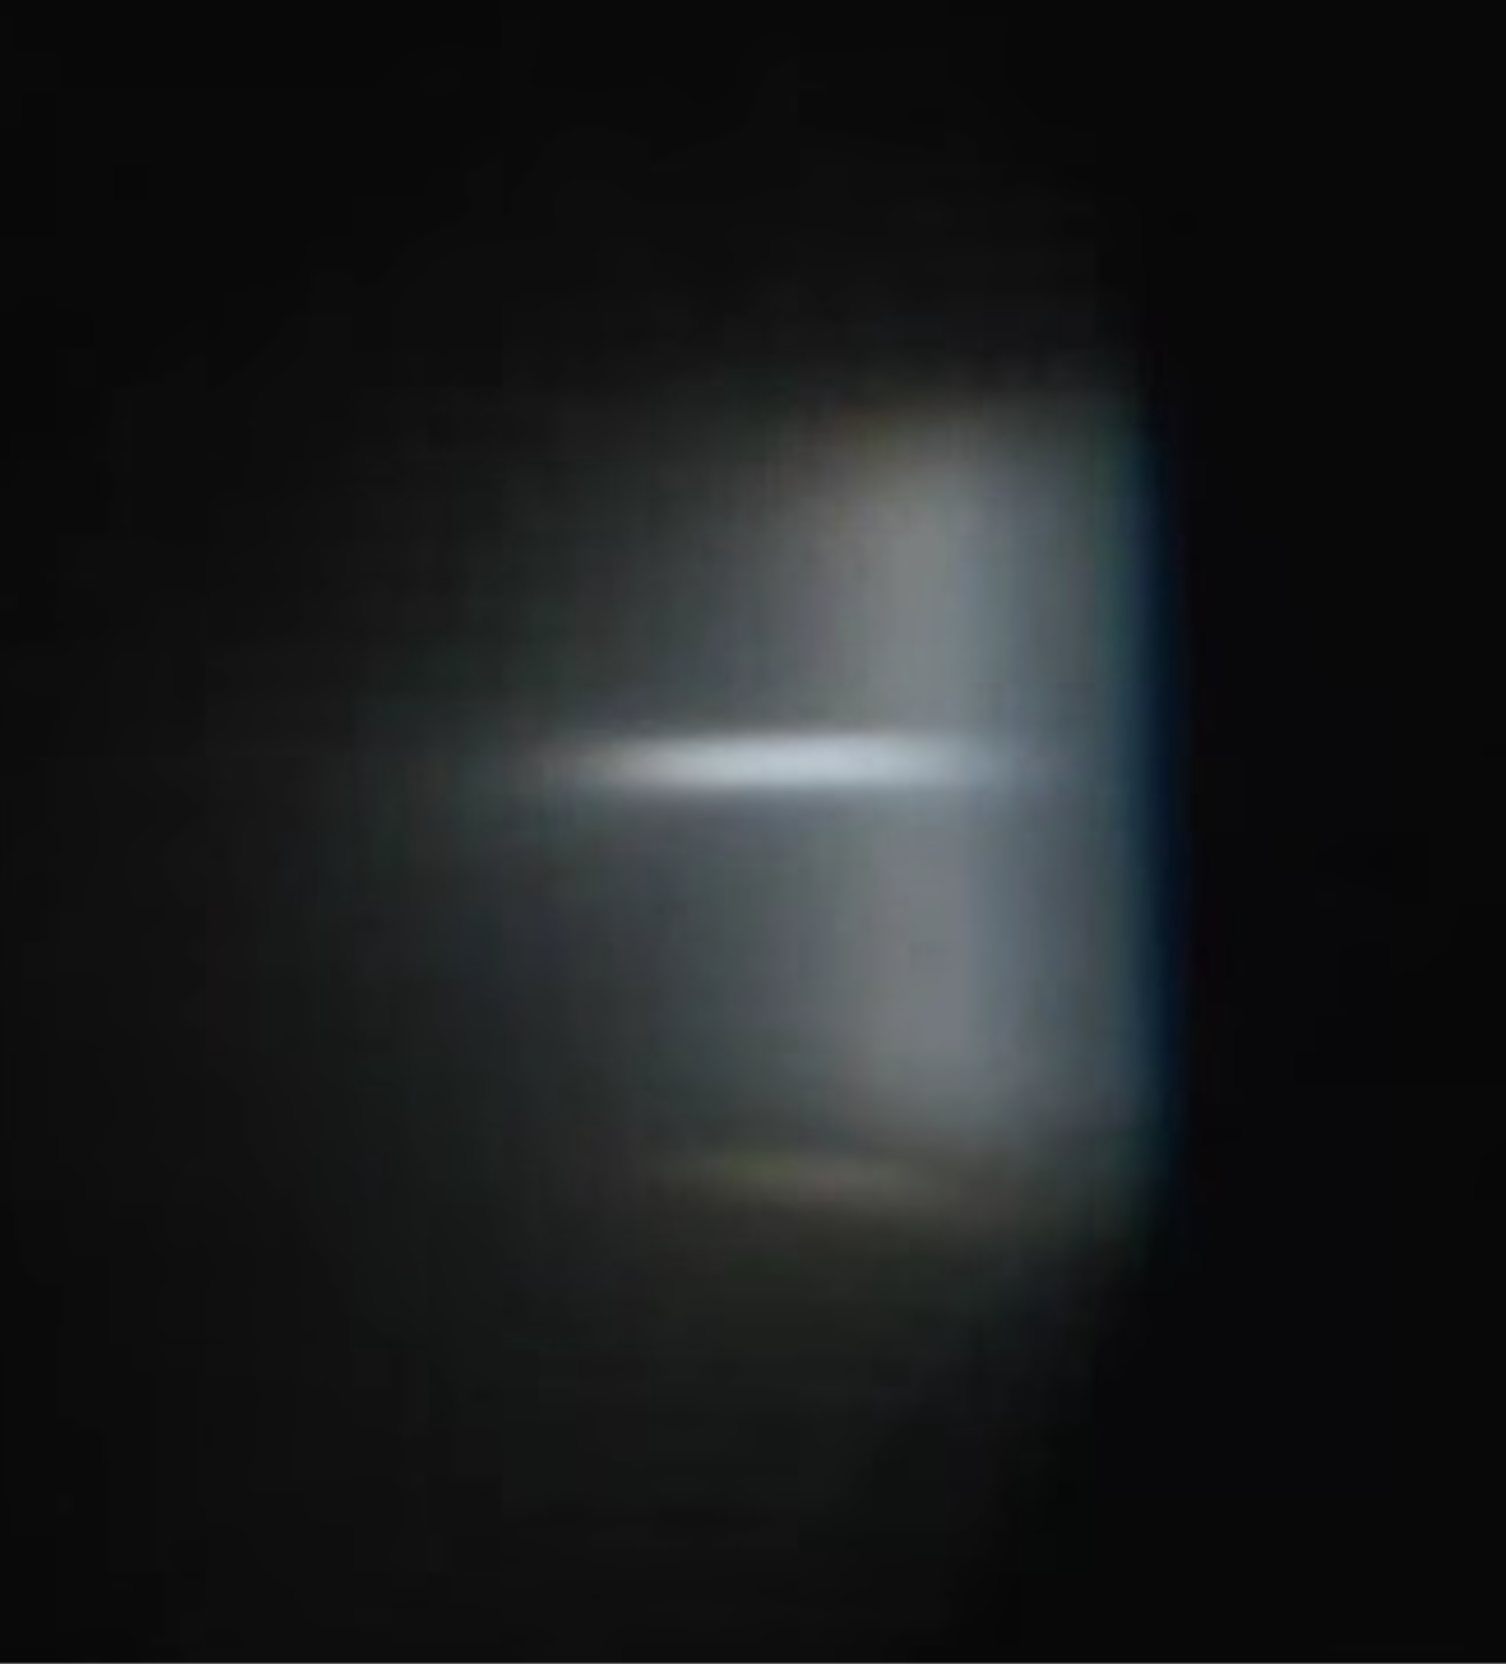
\includegraphics[keepaspectratio]{geometrical-optics/img/astighor_exp.png}}

}

\subcaption{\label{fig-astig-hor}Horizontal Focus}

\end{minipage}%

\caption{\label{fig-astigmatism}Astigmatism in optical systems. Left:
Schematic diagram illustrating how a tilted lens creates different focal
planes for rays in different meridional planes. The tangential
(vertical) and sagittal (horizontal) rays focus at different distances
from the lens. Middle: Experimental image showing the focusing of
vertical lines of a test object (letter ``F'') at one focal position.
Right: The same object at a different focal position where horizontal
lines are in focus. This demonstrates how astigmatism causes different
focal planes for vertical and horizontal features when a lens is tilted
relative to the optical axis. The inability to focus both orientations
simultaneously is a characteristic feature of astigmatic aberration.}

\end{figure}%

This distortion, i.e.~the elliptical shape of the focus has been used
advatageously in single molecule microscopy to locate their position
alsong the optical axis, which is typically a challenge for optical
microscopy.

\begin{tcolorbox}[enhanced jigsaw, breakable, toptitle=1mm, bottomrule=.15mm, colbacktitle=quarto-callout-note-color!10!white, title=\textcolor{quarto-callout-note-color}{\faInfo}\hspace{0.5em}{Astigmatism}, arc=.35mm, rightrule=.15mm, bottomtitle=1mm, opacityback=0, toprule=.15mm, coltitle=black, leftrule=.75mm, opacitybacktitle=0.6, colback=white, left=2mm, titlerule=0mm, colframe=quarto-callout-note-color-frame]

An optical aberration where rays from an off-axis point source focusing
in two perpendicular planes (meridional and sagittal) have different
focal lengths, resulting in image points that appear as ellipses
oriented either horizontally or vertically, depending on the observation
plane.

\end{tcolorbox}

\subsection{Distortions}\label{distortions}

Barrel or cushion shaped distortions in the image are found when
inserting apertures in the optical path. This results in the removal of
certain ray path ending up in field distortions.

\begin{figure}

\begin{minipage}{0.50\linewidth}

\centering{

\pandocbounded{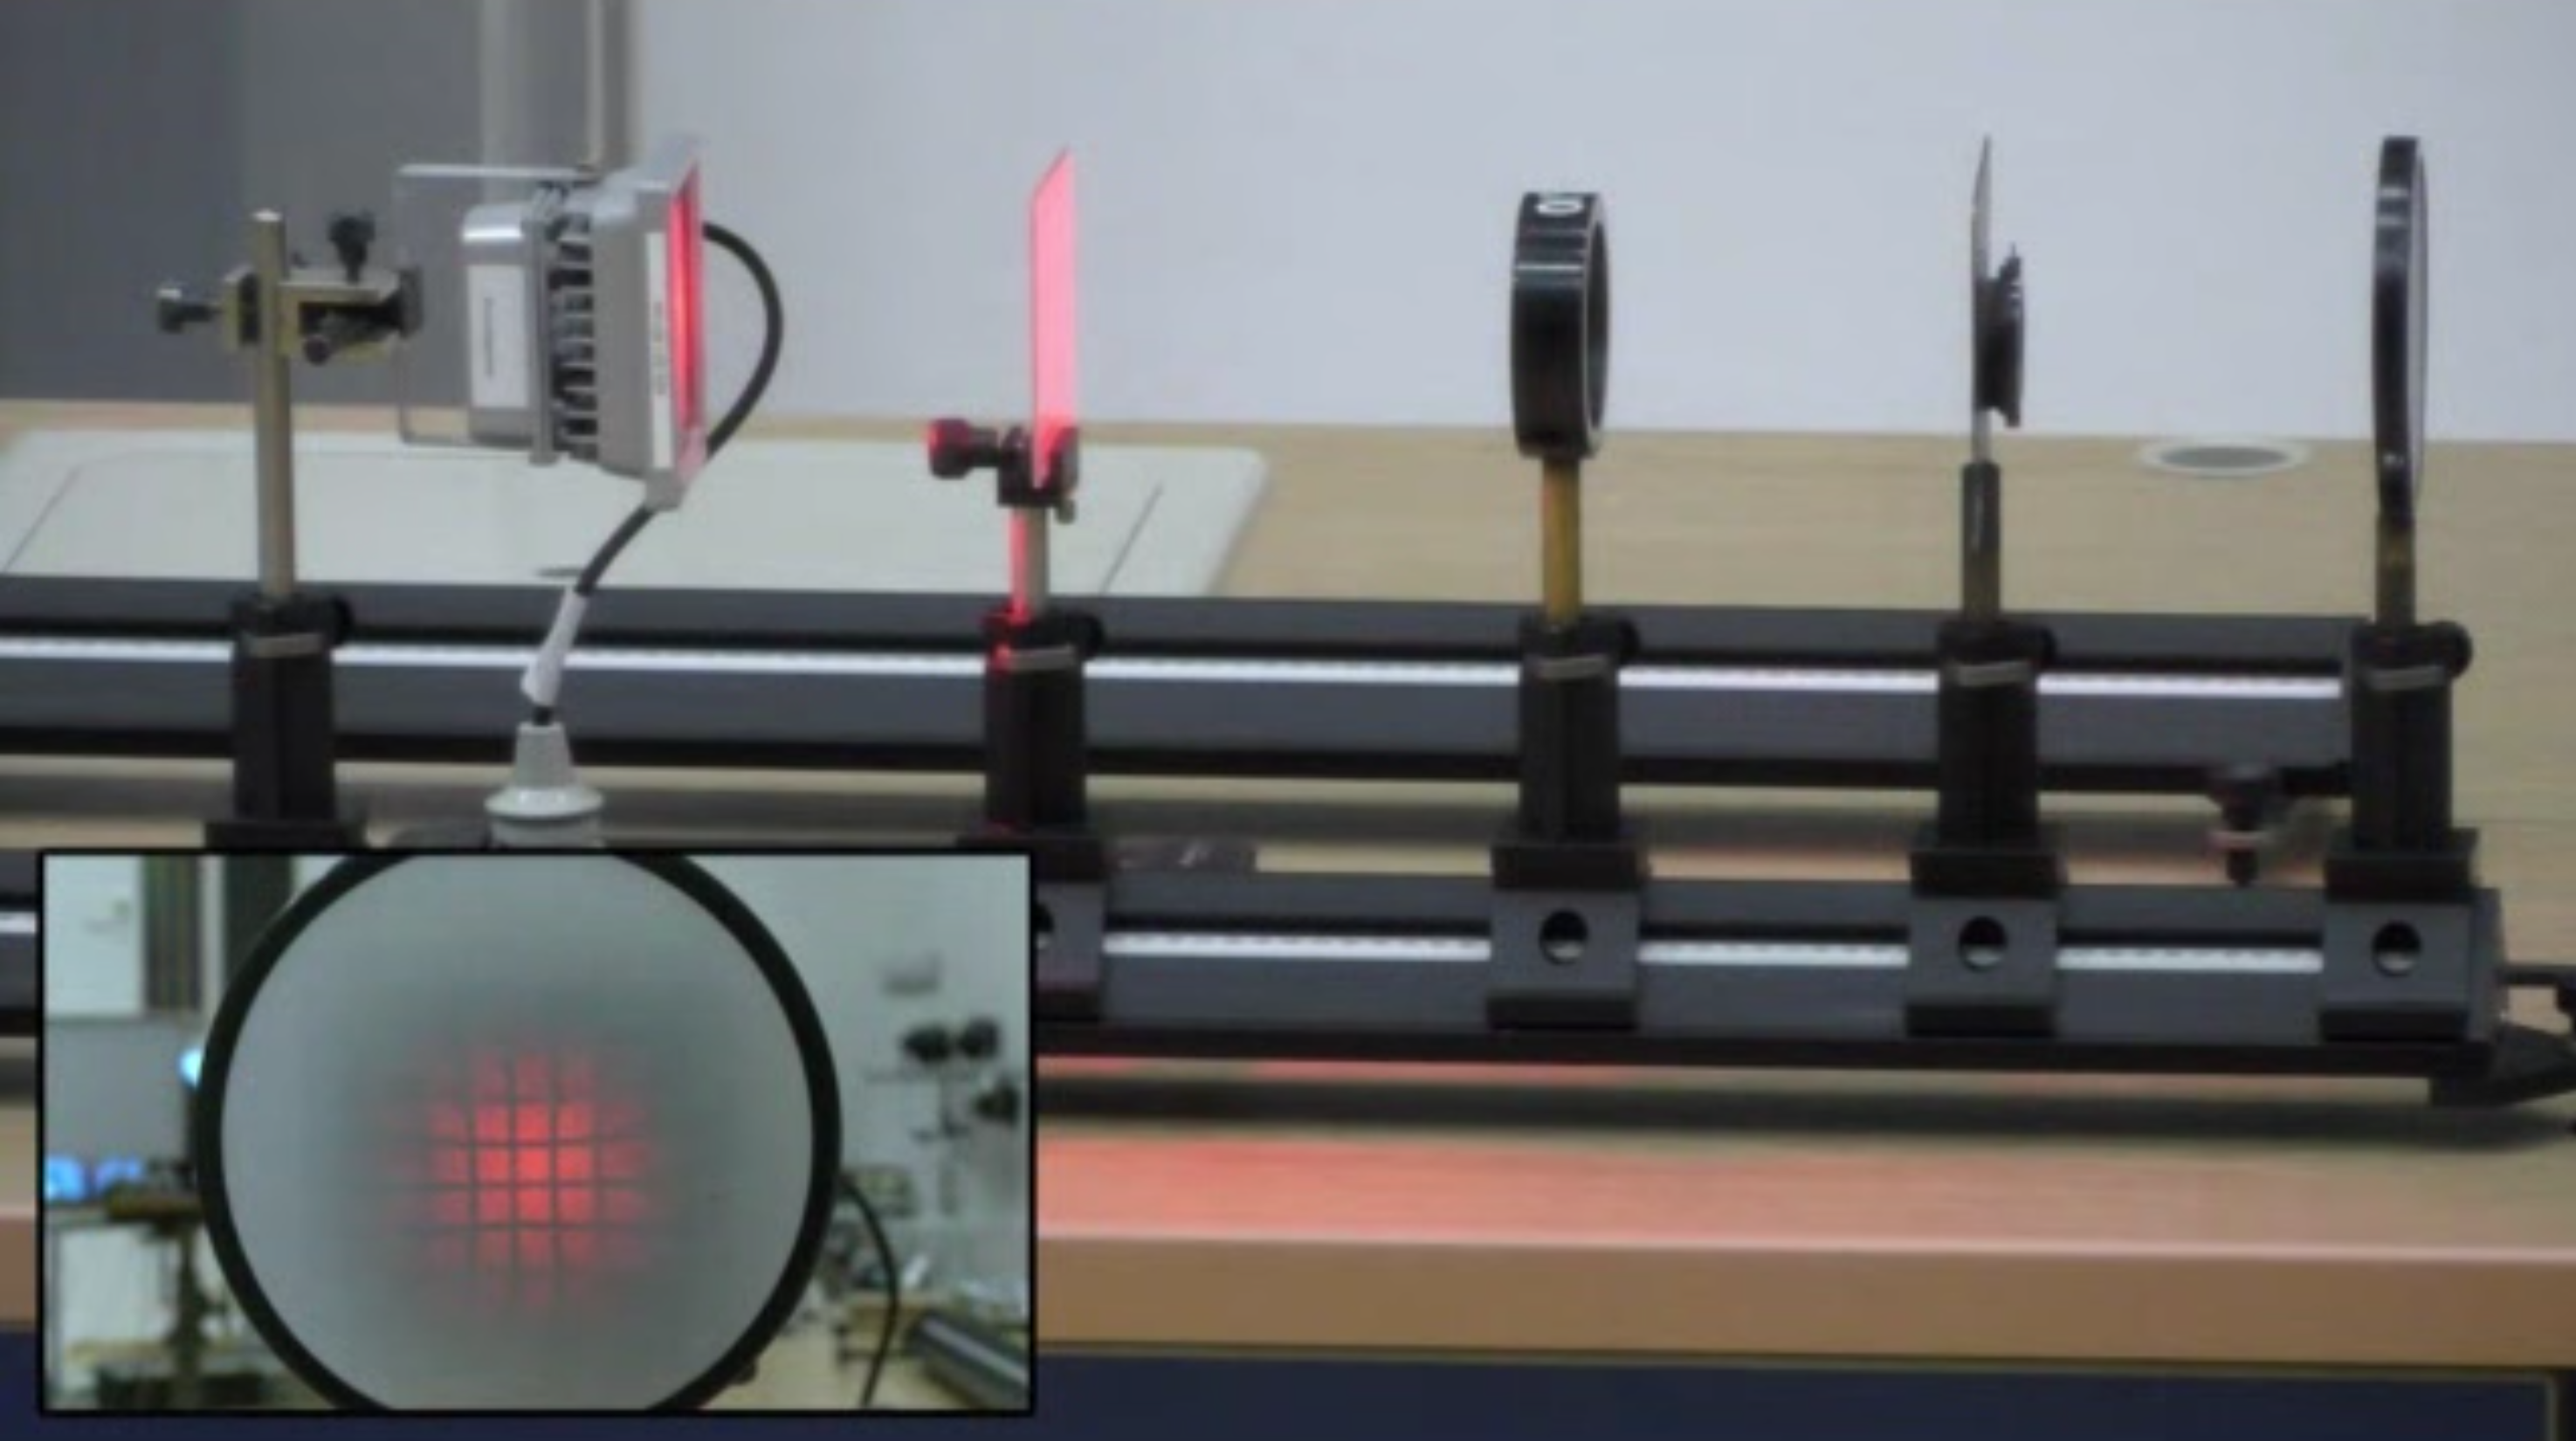
\includegraphics[keepaspectratio]{geometrical-optics/img/cushion_exp.png}}

}

\subcaption{\label{fig-cushion}Cushion Distortion}

\end{minipage}%
%
\begin{minipage}{0.50\linewidth}

\centering{

\pandocbounded{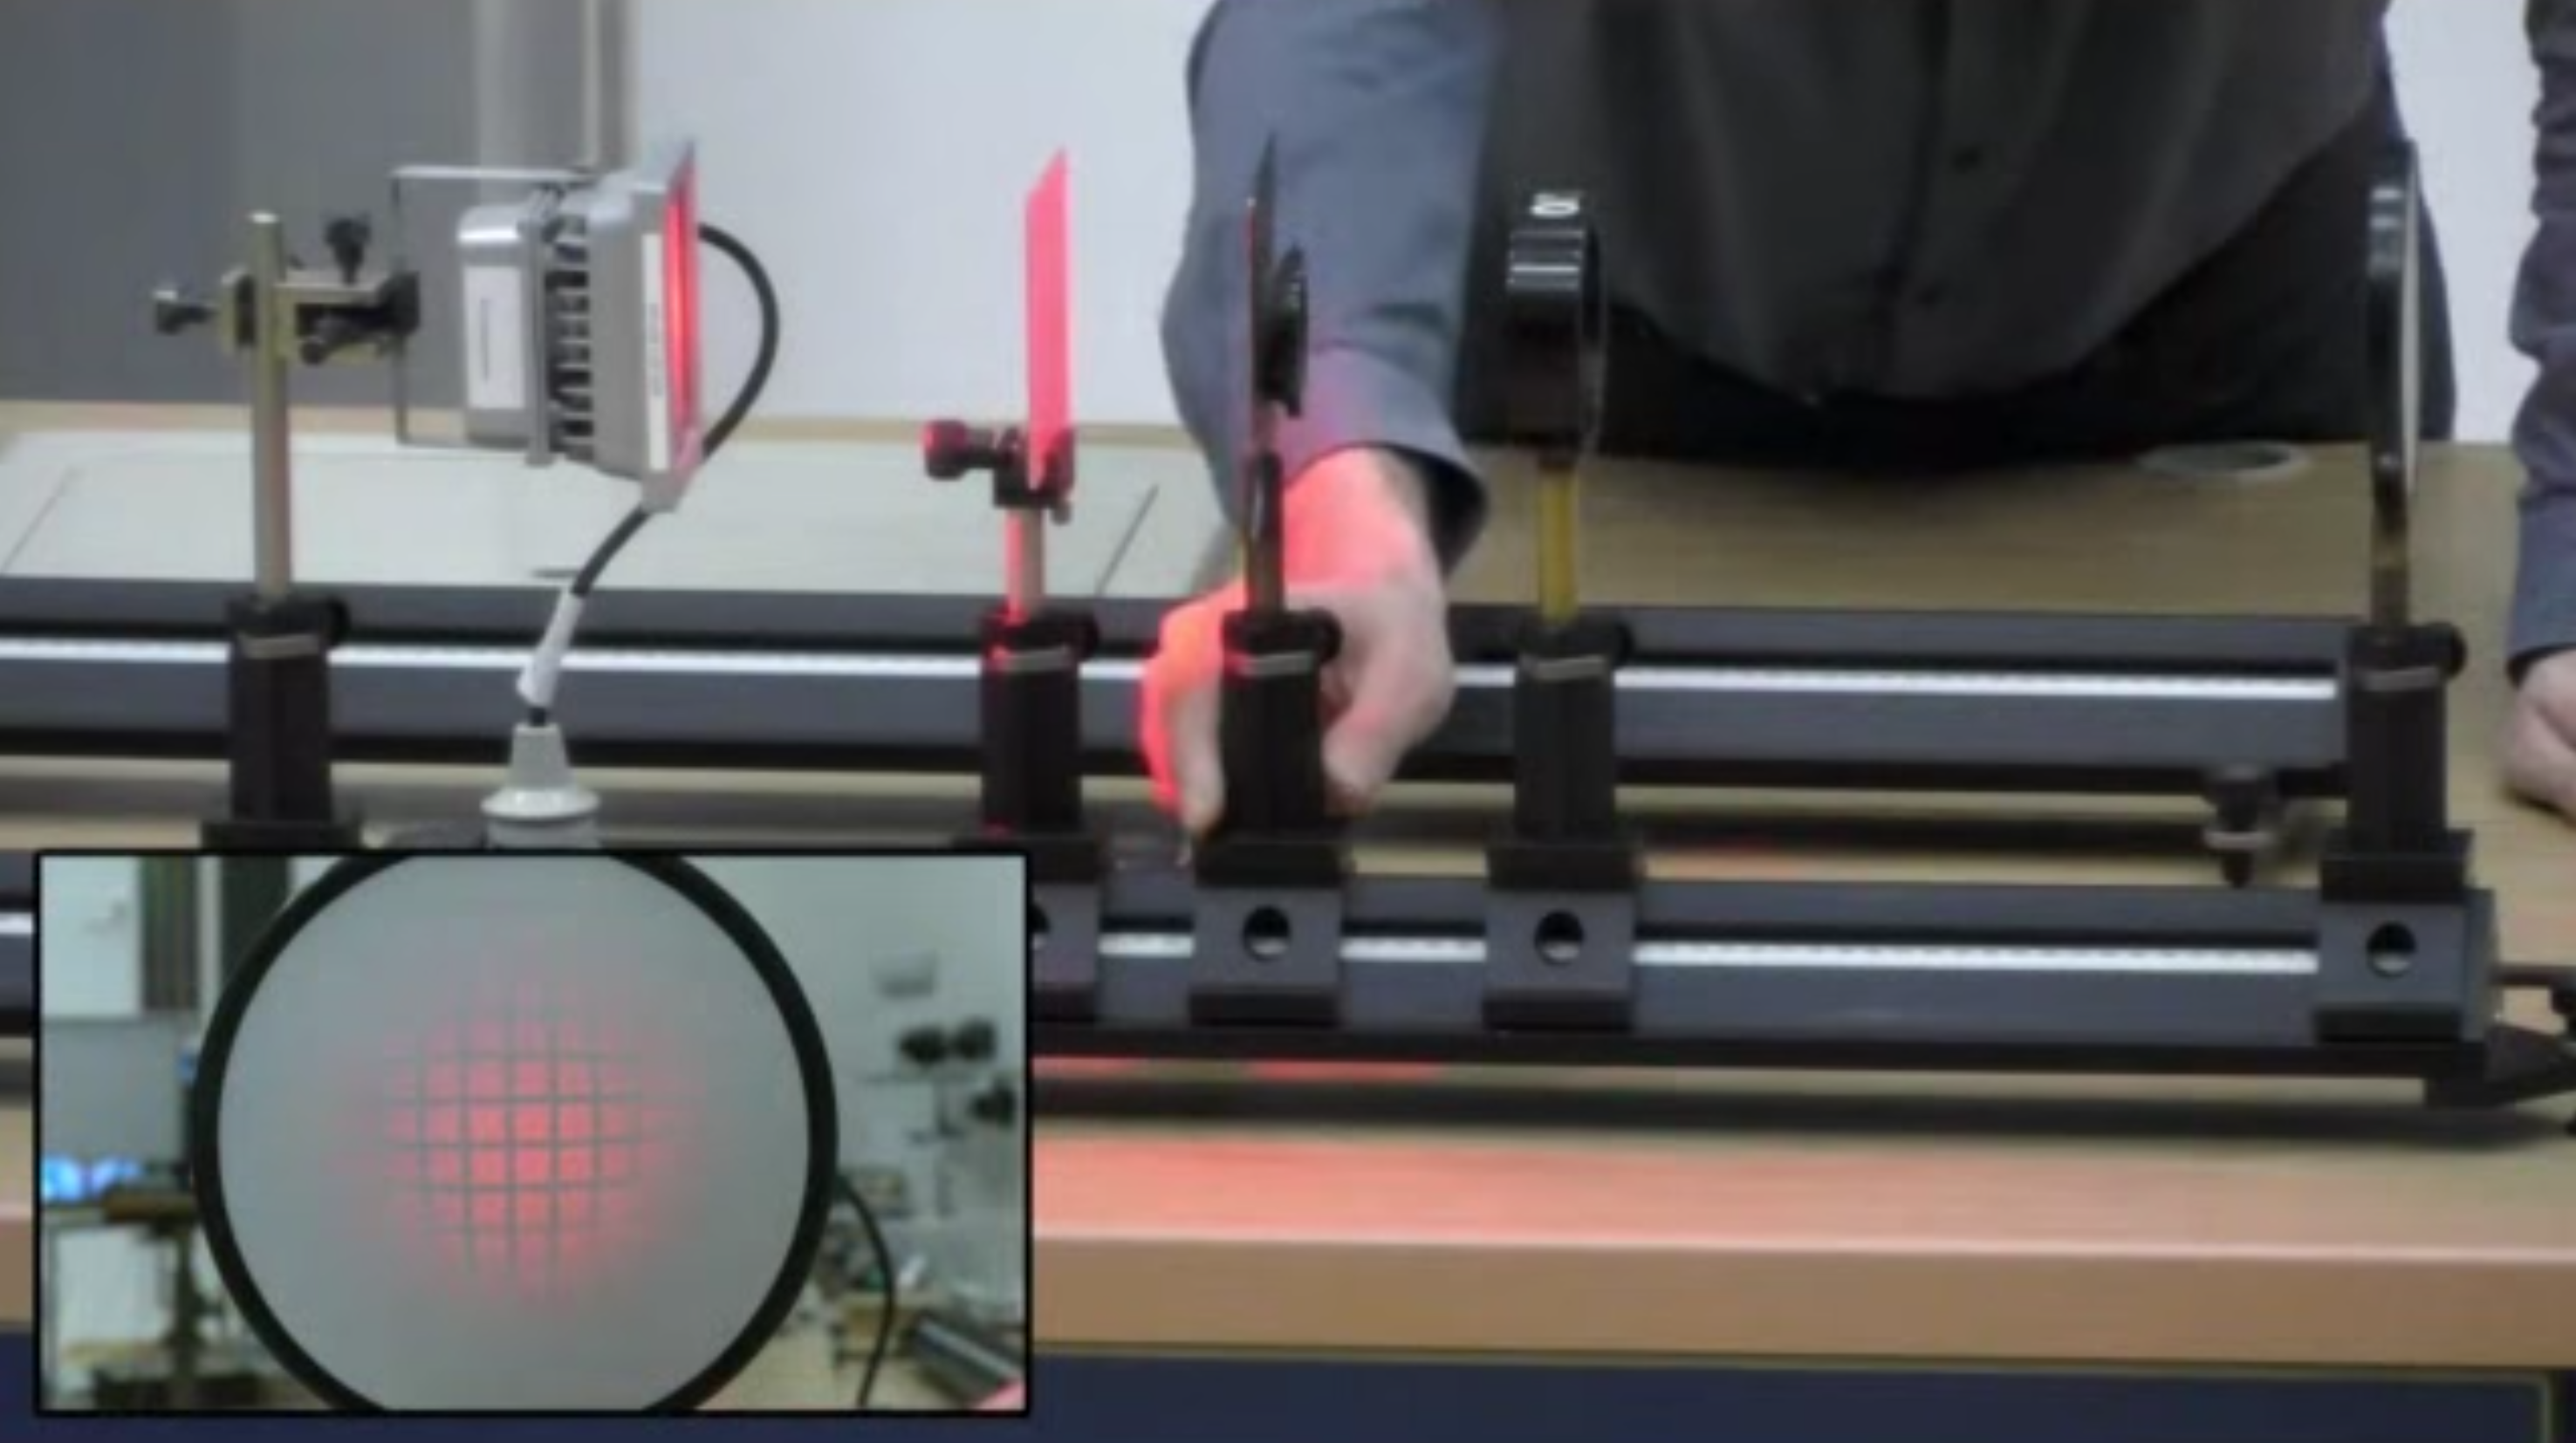
\includegraphics[keepaspectratio]{geometrical-optics/img/barrel_exp.png}}

}

\subcaption{\label{fig-barrel}Barrel Distortion}

\end{minipage}%

\caption{\label{fig-distortion}Geometric distortions in optical systems.
Left: Cushion (or pincushion) distortion, where the magnification
increases with distance from the optical axis, causing straight lines to
bow inward and creating a cushion-like appearance. Right: Barrel
distortion, where the magnification decreases with distance from the
optical axis, causing straight lines to bow outward, resembling the
shape of a barrel. These distortions maintain image sharpness but alter
the geometric shape of the image, particularly noticeable in
architectural photography or when imaging regular grid patterns.}

\end{figure}%

Geometric distortions arise from the position of the aperture relative
to the lens and its effect on ray paths. This mechanism can be
understood by analyzing how different rays contribute to image
formation:

When an aperture is placed behind the lens, rays that pass through
create an image point \(M_1\) that is farther from the optical axis than
the ideal image point \(M\) (where \(M\) is determined by the central
ray from object point \(A_0\)). As the object point moves farther from
the optical axis, the displacement between \(M_1\) and \(M\) increases
proportionally. This progressive displacement transforms a regular grid
pattern into a cushion (or pincushion) shape.

Conversely, when the aperture is placed in front of the lens, the
opposite effect occurs. The rays that pass through the aperture create
an image point closer to the optical axis than the ideal image point,
resulting in barrel distortion. The magnitude of this displacement also
increases with distance from the optical axis.

These theoretical predictions are confirmed by experimental
observations, where:

\begin{itemize}
\tightlist
\item
  A rear aperture produces cushion distortion, causing straight lines to
  bow inward
\item
  A front aperture produces barrel distortion, causing straight lines to
  bow outward
\end{itemize}

The severity of these distortions depends on both the aperture position
and the distance of object points from the optical axis.

\begin{figure}

\centering{

\pandocbounded{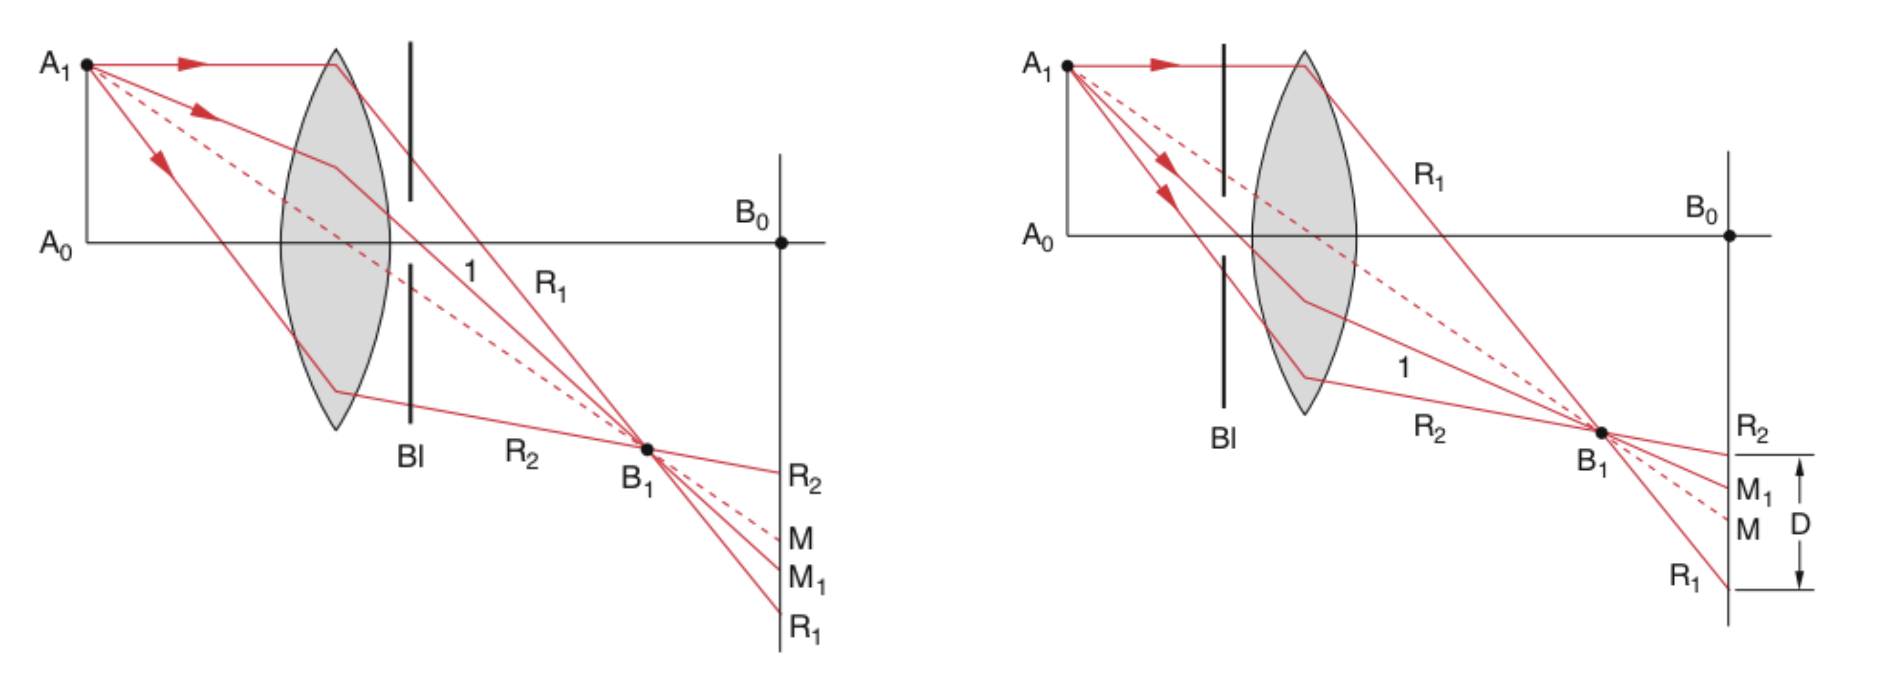
\includegraphics[keepaspectratio]{geometrical-optics/img/distortions.png}}

}

\caption{\label{fig-distortion-sketch}Cushion (left) and barrel (right)
type of distortions.}

\end{figure}%

\begin{tcolorbox}[enhanced jigsaw, breakable, toptitle=1mm, bottomrule=.15mm, colbacktitle=quarto-callout-note-color!10!white, title=\textcolor{quarto-callout-note-color}{\faInfo}\hspace{0.5em}{Cushion Distortion}, arc=.35mm, rightrule=.15mm, bottomtitle=1mm, opacityback=0, toprule=.15mm, coltitle=black, leftrule=.75mm, opacitybacktitle=0.6, colback=white, left=2mm, titlerule=0mm, colframe=quarto-callout-note-color-frame]

Cushion Distortion (also called Pincushion Distortion) - An optical
aberration where straight lines appear to bow inward toward the center
of the image, like the sides of a cushion or pincushion. This type of
distortion is typically seen in telephoto lenses and makes the center of
the image appear to be pinched inward.

\end{tcolorbox}

\begin{tcolorbox}[enhanced jigsaw, breakable, toptitle=1mm, bottomrule=.15mm, colbacktitle=quarto-callout-note-color!10!white, title=\textcolor{quarto-callout-note-color}{\faInfo}\hspace{0.5em}{Barrel Distortion}, arc=.35mm, rightrule=.15mm, bottomtitle=1mm, opacityback=0, toprule=.15mm, coltitle=black, leftrule=.75mm, opacitybacktitle=0.6, colback=white, left=2mm, titlerule=0mm, colframe=quarto-callout-note-color-frame]

Barrel Distortion - An optical aberration where straight lines appear to
bow outward from the center of the image, like a barrel shape. This type
of distortion is common in wide-angle lenses and makes the center of the
image appear to bulge outward.

\end{tcolorbox}

\begin{tcolorbox}[enhanced jigsaw, breakable, toptitle=1mm, bottomrule=.15mm, colbacktitle=quarto-callout-note-color!10!white, title=\textcolor{quarto-callout-note-color}{\faInfo}\hspace{0.5em}{Aberration Characterization and Zernike Polynomials}, arc=.35mm, rightrule=.15mm, bottomtitle=1mm, opacityback=0, toprule=.15mm, coltitle=black, leftrule=.75mm, opacitybacktitle=0.6, colback=white, left=2mm, titlerule=0mm, colframe=quarto-callout-note-color-frame]

The Zernike polynomials are a set of orthonormal polynomials that are
widely used in optics to describe wavefronts and to characterize optical
aberrations. As we did not discuss wavefronts and waves yet, this is a
more advanced topic here and only for information. Zernike polynomials
are defined over the unit disk and are particularly useful because they
are orthogonal under the inner product, which involves integration over
the unit circle. This makes them suitable for decomposing a wavefront
into a sum of orthogonal modes, each representing a different type of
aberration.

The general form of the Zernike polynomials can be expressed in polar
coordinates \((\rho, \phi)\), where \(\rho\) is the radial distance from
the origin (normalized to the unit circle) and \(\phi\) is the azimuthal
angle. The Zernike polynomials are defined as:

\[
Z_n^m(\rho, \phi) =
\begin{cases}
R_n^m(\rho) \cos(m\phi) & \text{for } m \geq 0 \\
R_n^{|m|}(\rho) \sin(|m|\phi) & \text{for } m < 0
\end{cases}
\]

where \(n\) is a non-negative integer, \(m\) is an integer such that
\(n - |m|\) is even and \(0 \leq |m| \leq n\), and \(R_n^m(\rho)\) is
the radial polynomial given by:

\[
R_n^m(\rho) = \sum_{k=0}^{\frac{n-m}{2}} \frac{(-1)^k (n-k)!}{k! \left(\frac{n+m}{2} - k\right)! \left(\frac{n-m}{2} - k\right)!} \rho^{n-2k}
\]

The radial polynomials \(R_n^m(\rho)\) are only dependent on the radial
distance \(\rho\), and they modulate the angular functions
\(\cos(m\phi)\) and \(\sin(|m|\phi)\) that describe the azimuthal
variation of the wavefront.

The Zernike polynomials are indexed in several ways, with one common
method being the Noll index, which provides a single index \(j\) to each
polynomial. Another method uses the pair \((n, m)\) to index the
polynomials, where \(n\) indicates the order of the polynomial and \(m\)
its azimuthal frequency.

These polynomials are particularly useful in optics and ophthalmology
for describing the shape of optical wavefronts and the aberrations of
optical systems, including the human eye. They allow for the
decomposition of a complex wavefront into simpler, orthogonal
components, each corresponding to a specific type of aberration, such as
defocus, astigmatism, coma, etc.

The plots below visualize the Zernike Polynomials up to a certain order.

\pandocbounded{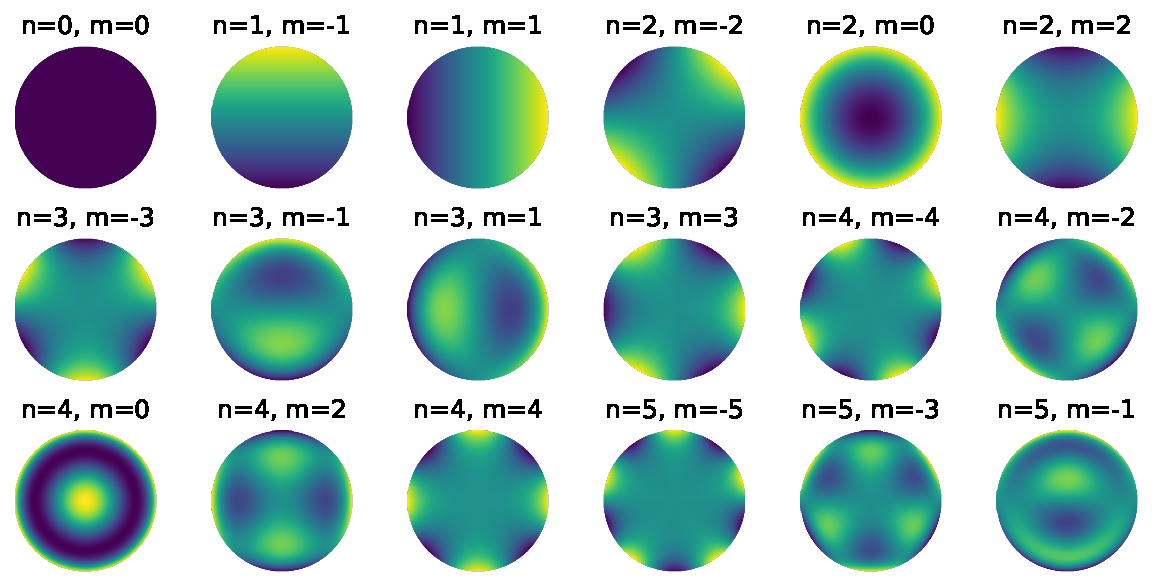
\includegraphics[keepaspectratio]{geometrical-optics/Imaging Errors_files/figure-pdf/cell-4-output-1.pdf}}

\end{tcolorbox}

\chapter{Rainbow}\label{rainbow}

As the last topic of the optical elements we would like to have a look
at a phenomenon, which has nothing to do with optical elements but is
fun and just fits to the topic of dispersion. We will explore the
rainbow and in addition a DIY version, the glassbow.

\subsection{Historical Background}\label{historical-background}

The rainbow has fascinated humans throughout history, but its first
scientific explanation came from René Descartes in 1637. Using geometric
optics, he explained how sunlight is reflected and refracted by
spherical water droplets to create the bow shape. However, Descartes
could not explain the colors. It was Isaac Newton who, through his
experiments with prisms and understanding of dispersion, provided the
complete explanation of the rainbow's colors in 1672. Newton showed that
white sunlight consists of different colors that are refracted at
slightly different angles due to dispersion.

\section{Single Drop Analysis}\label{single-drop-analysis}

To understand the rainbow we will have first a look at the reflection of
rays from a single droplet.

\begin{figure}[H]

{\centering 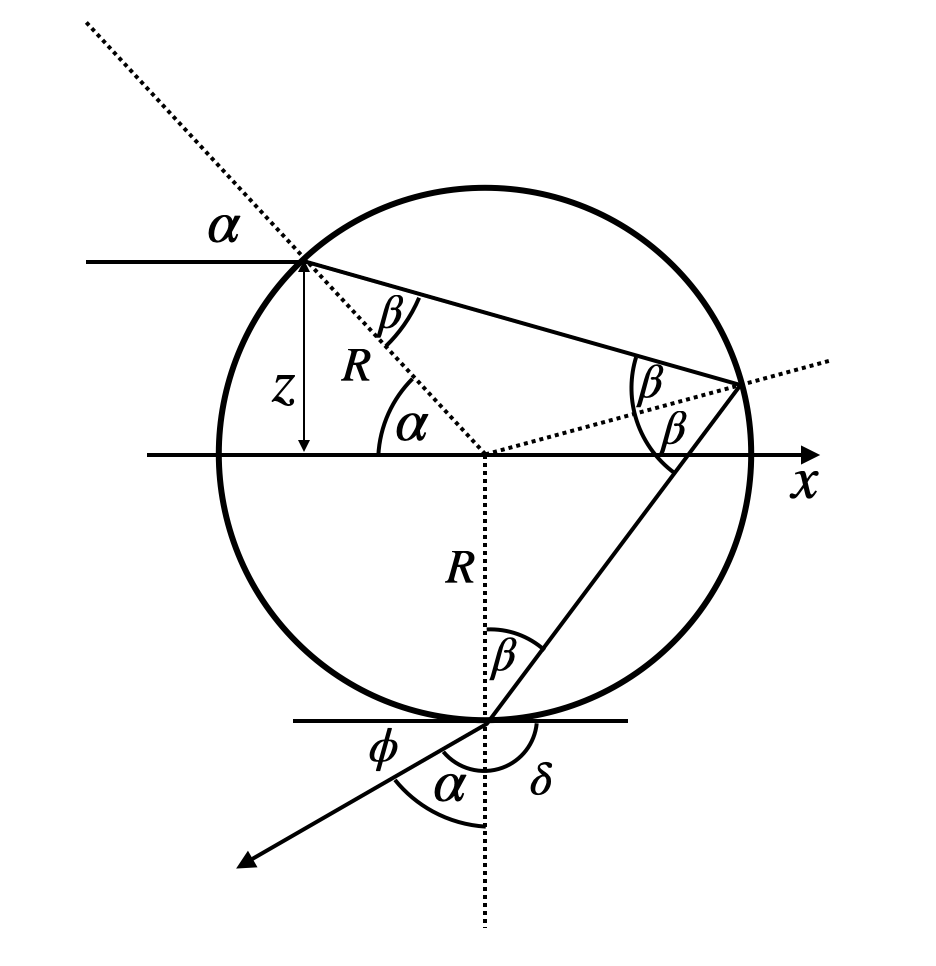
\includegraphics[width=0.4\linewidth,height=\textheight,keepaspectratio]{geometrical-optics/img/rainbow.png}

}

\caption{Reflection of rays in a single drop}

\end{figure}%

In the sketch above a light ray of white light is entering the droplet
under an angle \(\alpha\) to the surface normal on the top. The ray is
refracted and enters the droplet under an angle \(\beta\) to the surface
normal. The angle can be calculated from Snell's law

\[n_{\rm air}\sin(\alpha)=n_{\rm water}\sin(\beta).\]

Inside the droplet, the ray is now hitting the water/air surface at the
backside from which it gets reflected. There, the incident angle is also
\(\beta\) and the ray is reflected under an angle \(\beta\) as well. At
that point, most of the light will, however, exit the drop on the
backside, so that only a small fraction is reflected and traveling
further to hit a second time the water/air surface at the angle
\(\beta\). The light refracted out at that point leaves the droplet
under an angle \(\alpha\) with the surface normal due to the
reversiblity of the light path. We are, however, interested in the angle
\(\phi\) that the ray makes with the incident direction.

This angle \(\phi\) can be calculated from the above sketch to be

\[\phi=4\beta-2\alpha.\]

Since

\[\beta=\sin^{-1}\left (\frac{n_{\rm air}}{n_{\rm water}}\sin(\alpha) \right)\]

such that finally

\[\phi=4\sin^{-1}\left (\frac{n_{\rm air}}{n_{\rm water}}\sin(\alpha) \right)-2\alpha\]

So let us have a look at this dependence of the deflection angle as a
function of the incidence angle.

\begin{figure}[H]

{\centering \pandocbounded{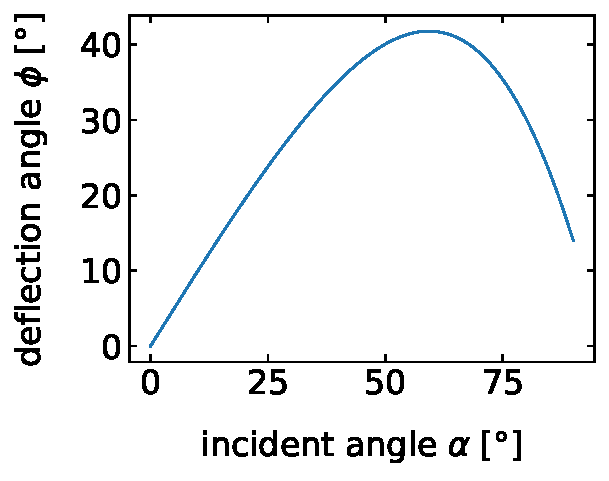
\includegraphics[keepaspectratio]{geometrical-optics/Rainbow_files/figure-pdf/cell-3-output-1.pdf}}

}

\caption{Deflection angle of a light ray in a water droplet as a
function of the incidence angle. The refractive index of water is taken
from the data file \texttt{H2O.csv}.}

\end{figure}%

The dependence seems to show a maximum deflection angle at an incidence
angle of around \(\alpha=60^{\circ}\). This is an important finding, as
the whole appearance of the rainbow depends on that.

\begin{verbatim}
Maximum deflection angle  41.78815648670841
\end{verbatim}

\subsection{Color Formation and
Dispersion}\label{color-formation-and-dispersion}

The color of the rainbow is the result of the fact that the maximum
deflection angle depends on the color of the light due to the
dispersion. Since we have a refraction, reflection and another
refraction, the largest maximum deflection angle is observed for red
light, while the smallest one appears for blue light. The diagrams below
show this result, which is in general true for materials with normal
dispersion.

\begin{figure}[H]

{\centering \pandocbounded{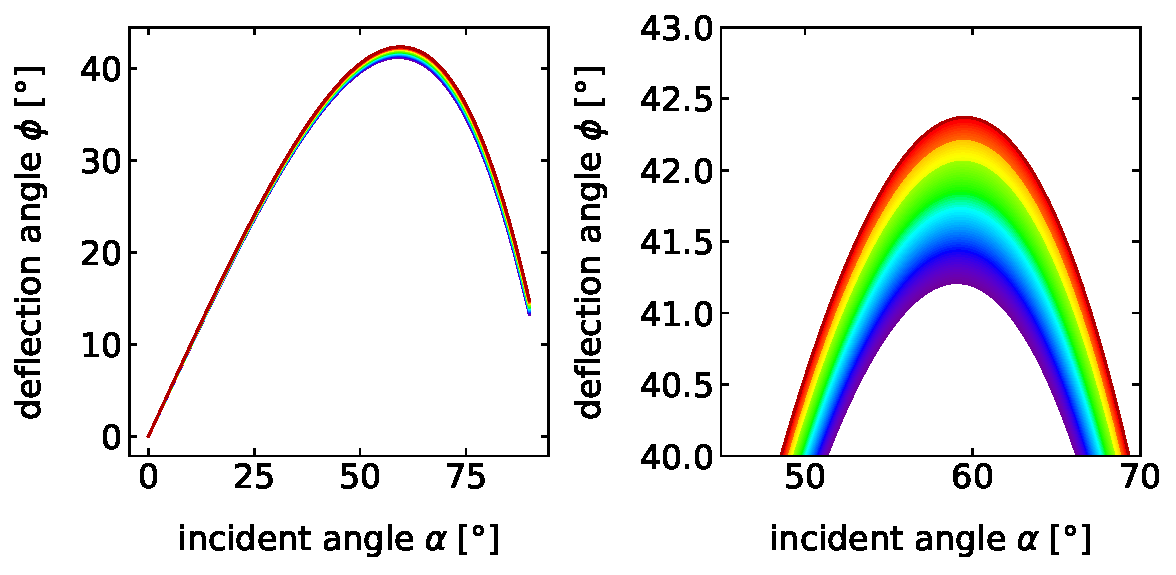
\includegraphics[keepaspectratio]{geometrical-optics/Rainbow_files/figure-pdf/cell-5-output-1.pdf}}

}

\caption{Caption}

\end{figure}%

This order of the colors is actually true for all incident angles, which
raises the question, why the rainbow is actually colored. The blue color
of a certain incidence angle would actually overlap with the green color
of a different incidence angle and the red color of an even different
incidence angle. If you select a specific outgoing angle under which you
observe the rainbow, let us say \(41^{\circ}\), then you find under this
observation angle all color and, therefore, should observe always white
light.

This is actually true if you look at the inside of a rainbow. You
clearly recognize that inside the rainbow it is much brighter than
outside. Yet when you reach the maximum angle of each color, you have a
region, where even for larger angles for the incidence angles, the
deflection angle does not change. Thus, if you assume you send in rays
at constantly spaced incidence angles, you will have more rays with a
deflection angle close to the maximum. The diagram below just counts the
number of deflection angles in the different for each color and you
clearly see that around the maximum deflection angles for each color you
have a strong peak.

\begin{figure}[H]

{\centering \pandocbounded{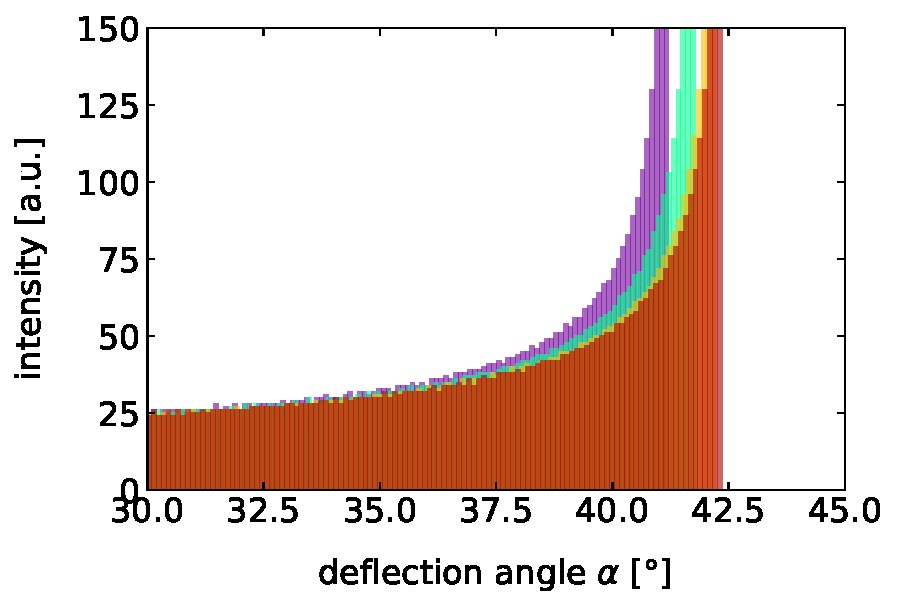
\includegraphics[keepaspectratio]{geometrical-optics/Rainbow_files/figure-pdf/cell-6-output-1.pdf}}

}

\caption{Histogram of the deflection angle of light rays in a water
droplet for different colors. The refractive index of water is taken
from the data file \texttt{H2O.csv}.}

\end{figure}%

Thus, around each droplet on the sky, there is a cone of deflected light
reflected back from the sun. On the outside of that cone is red light
under an angle of almost \(42^{\circ}\) while on the inside edge we find
blue light and finally white light (see left image below). We just have
to connect that to the observer now. This is shown in the right sketch.
The rainbow, therefore, results from the fact that we look at different
height at different edges of the cone.

\begin{figure}

\begin{minipage}{0.50\linewidth}

\centering{

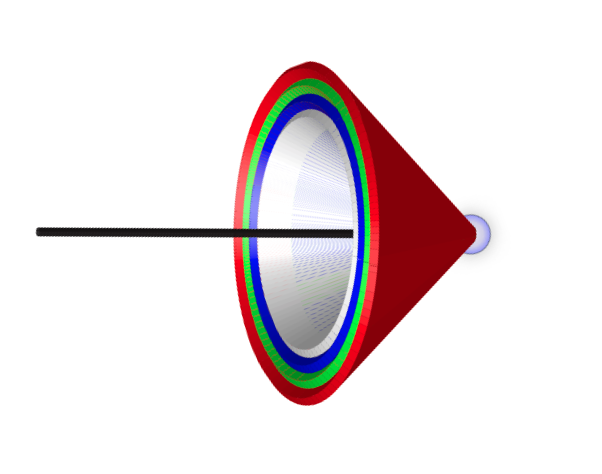
\includegraphics[width=1\linewidth,height=\textheight,keepaspectratio]{geometrical-optics/img/cone.png}

}

\subcaption{\label{fig-cone}Deflection cones}

\end{minipage}%
%
\begin{minipage}{0.50\linewidth}

\centering{

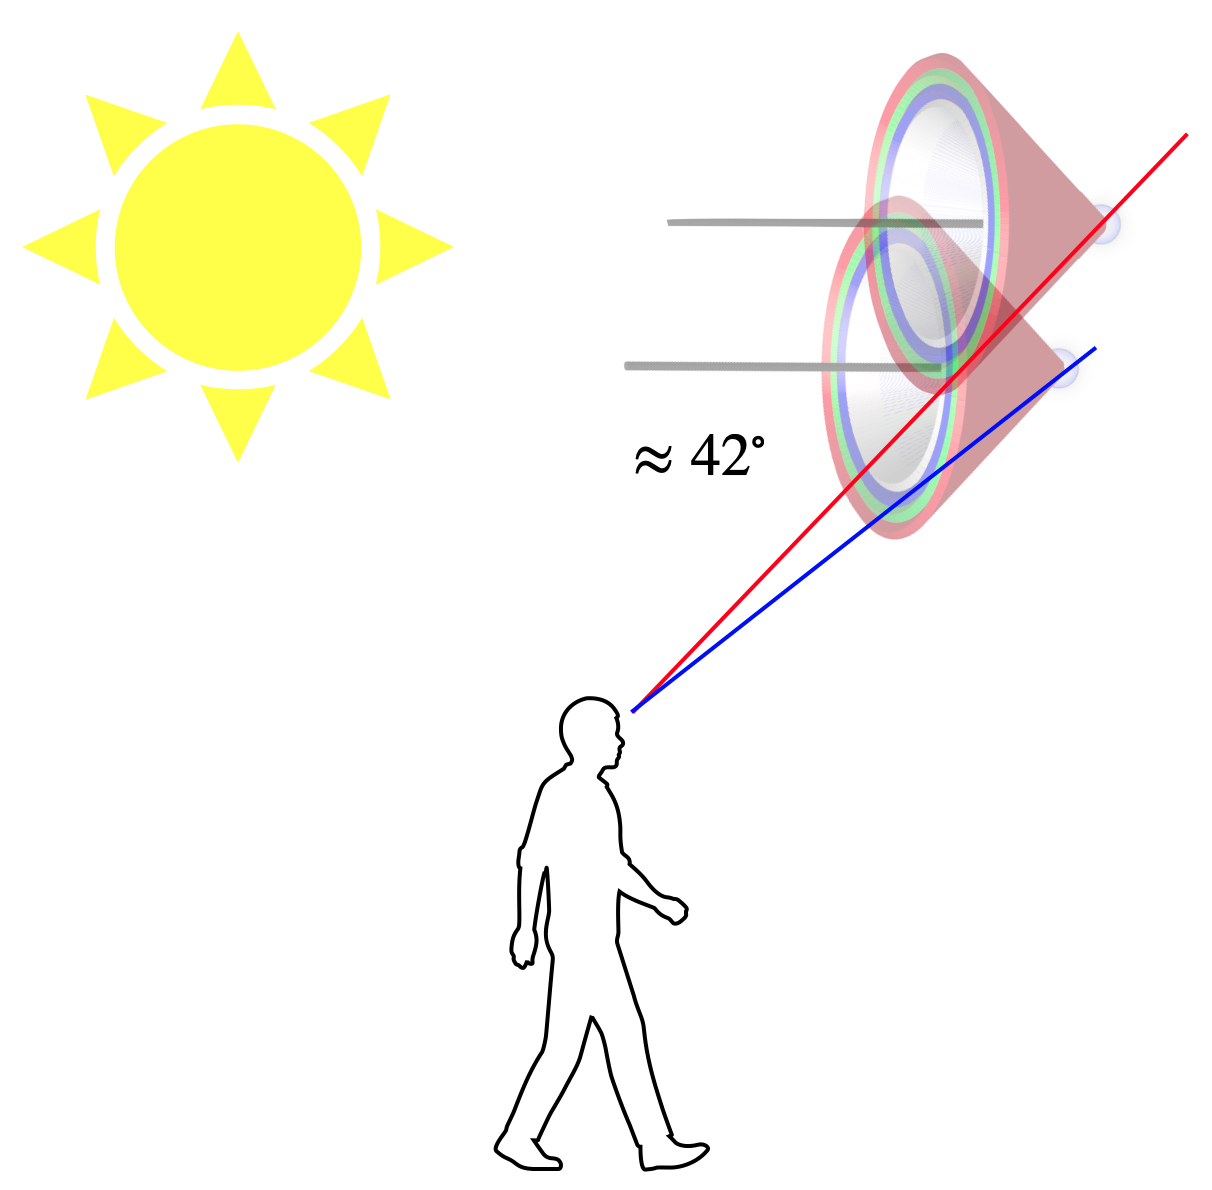
\includegraphics[width=1\linewidth,height=\textheight,keepaspectratio]{geometrical-optics/img/observation.png}

}

\subcaption{\label{fig-observation}Resulting rainbow}

\end{minipage}%

\caption{\label{fig-rainbow-formation}Deflection cones of different
colors on a single drop in a rainbow (left) and the resulting rainbow as
observed from these cones (right).}

\end{figure}%

\subsection{Primary and Secondary
Rainbows}\label{primary-and-secondary-rainbows}

The photos below show a remarkable example of both primary and secondary
rainbows. Between these two bows, a careful observer will notice a
darker region known as Alexander's dark band, first described by
Alexander of Aphrodisias in 200 AD. This dark band occurs because no
light is scattered back to the observer at angles between approximately
\(42^{\circ}\) (maximum angle of primary rainbow) and \(50^{\circ}\)
(minimum angle of secondary rainbow).

\begin{figure}[H]

{\centering \pandocbounded{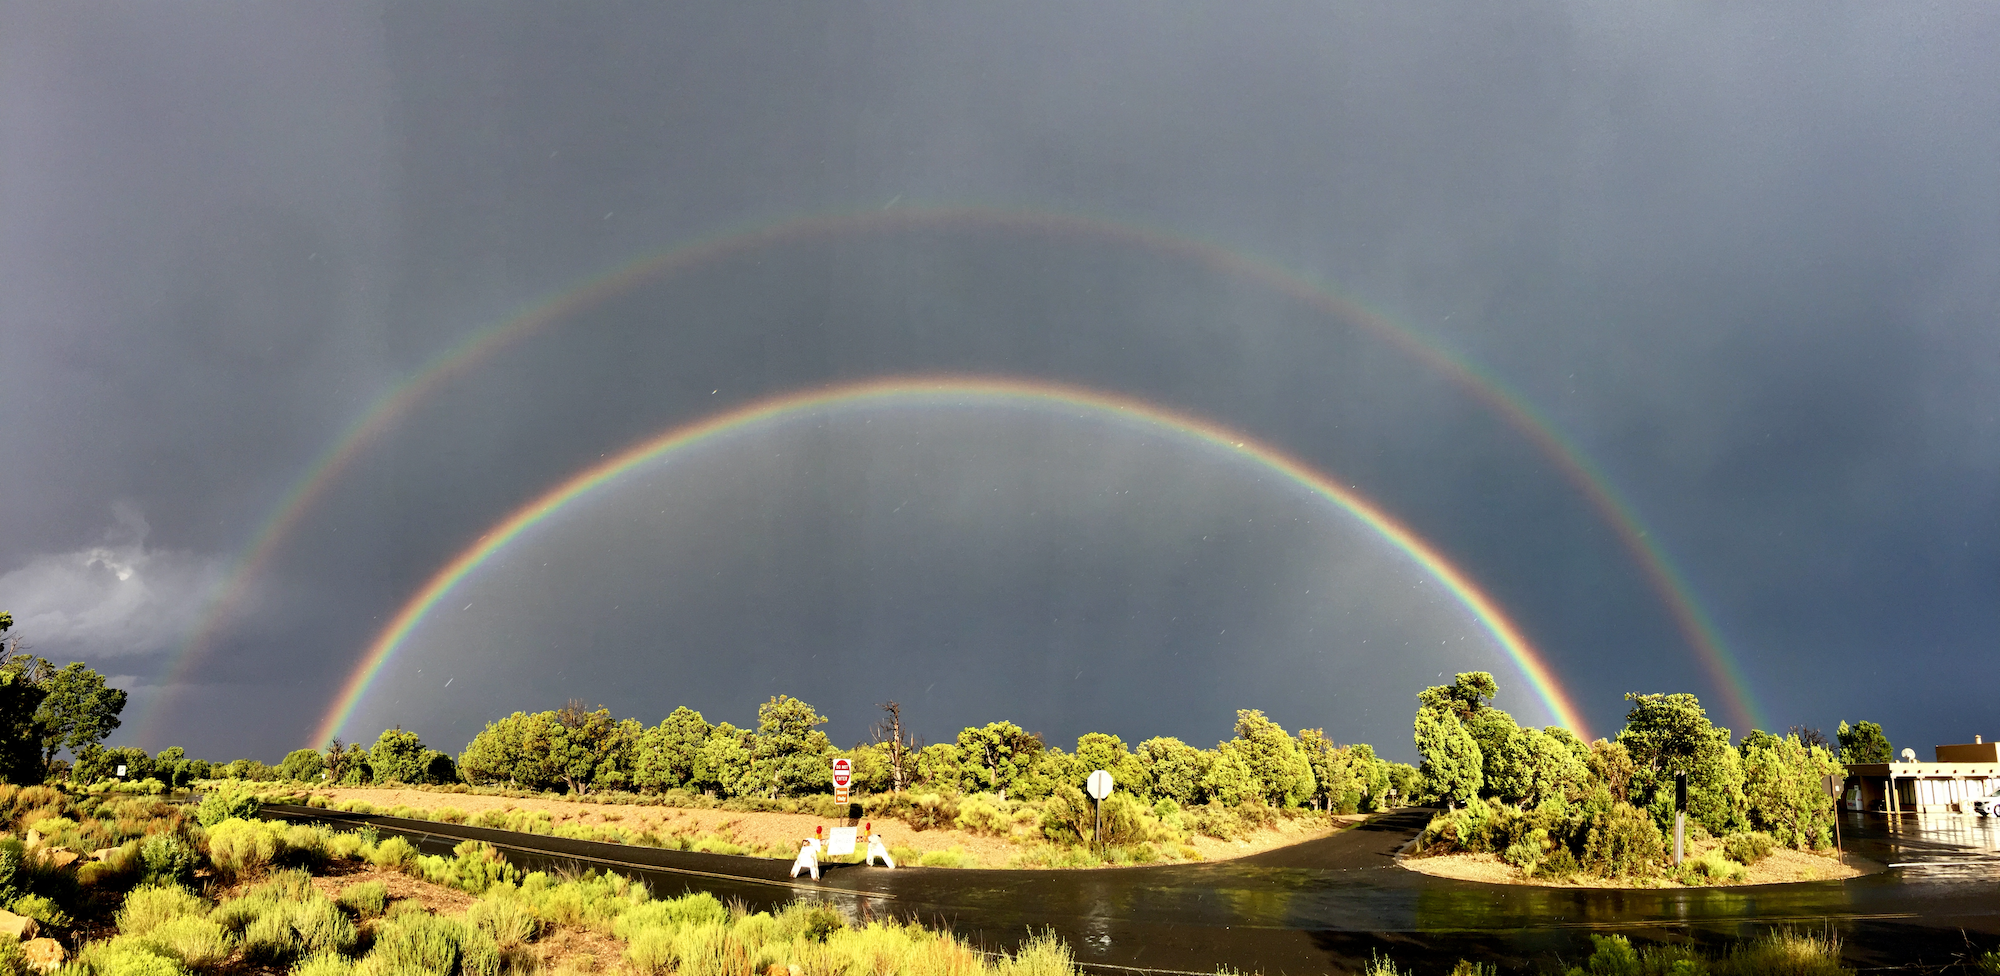
\includegraphics[keepaspectratio]{geometrical-optics/img/rainbow_full.png}}

}

\caption{Double rainbow over Grand Canyon. (Frank Cichos)}

\end{figure}%

The primary rainbow results from one internal reflection within each
water droplet, while the secondary rainbow involves two internal
reflections. This double reflection explains both the reversed color
order and the reduced brightness of the secondary rainbow, as each
reflection decreases the light intensity.

\begin{figure}[H]

{\centering \pandocbounded{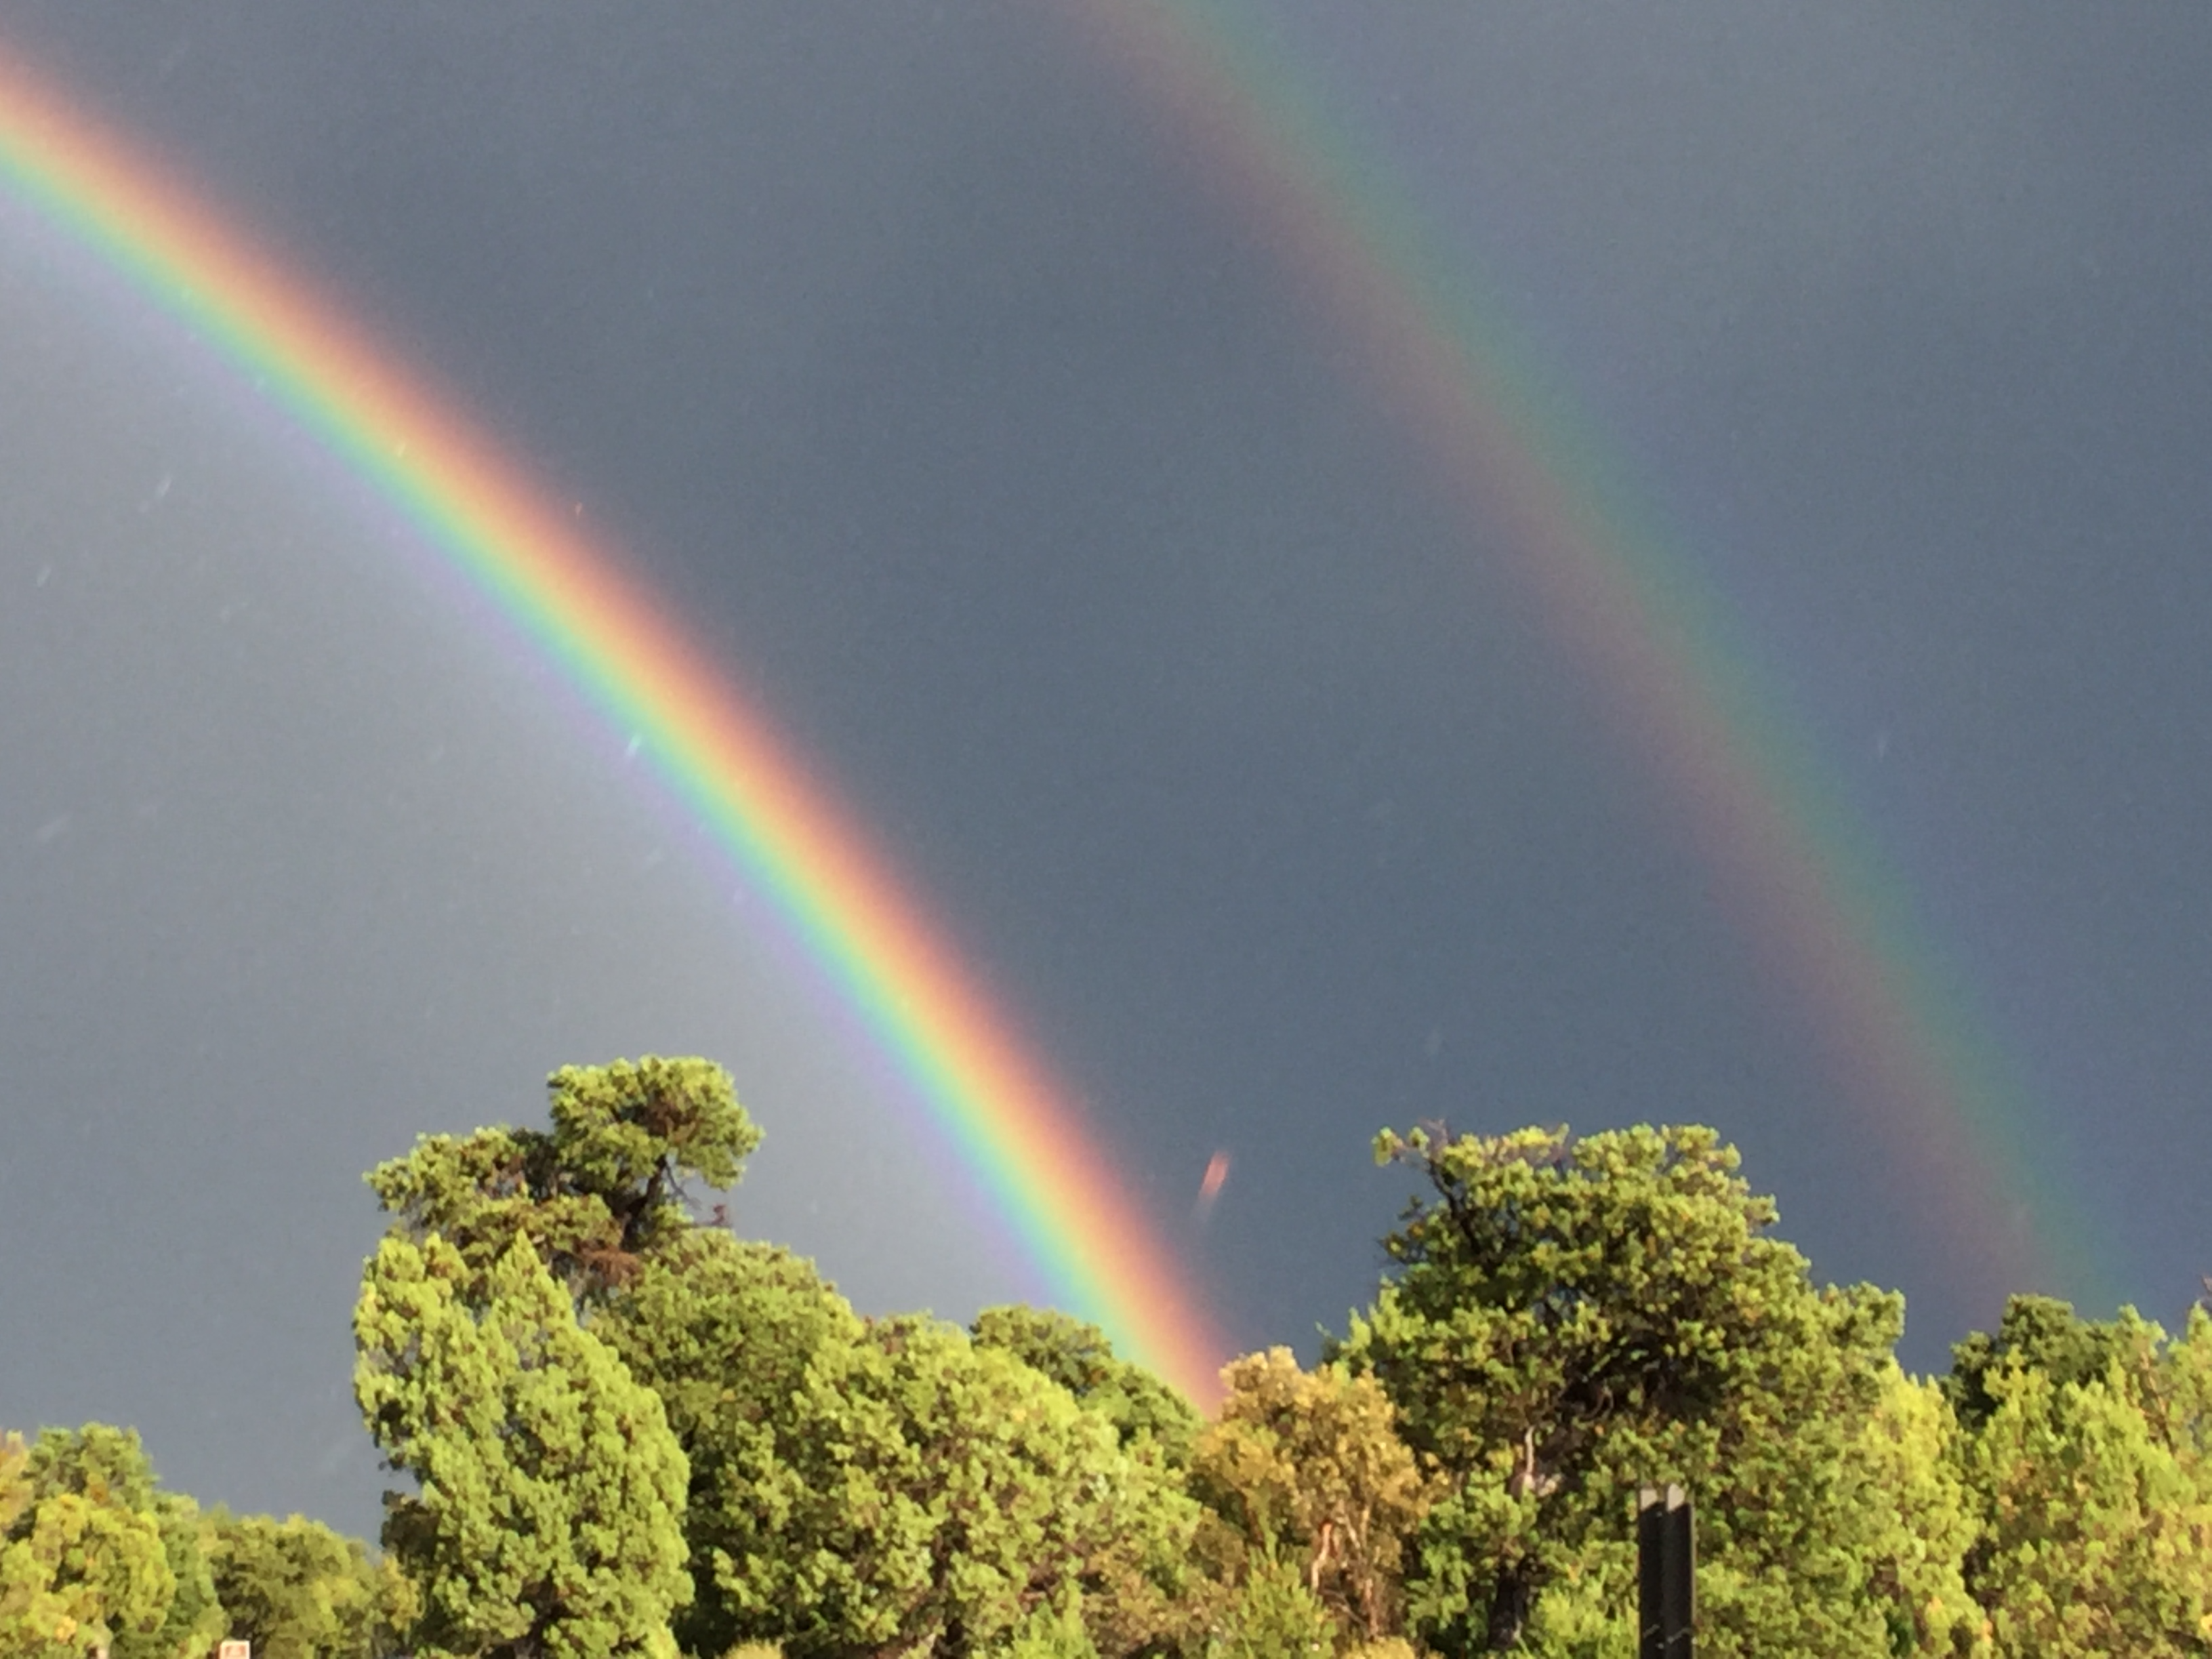
\includegraphics[keepaspectratio]{geometrical-optics/img/rainbow_gczoom.png}}

}

\caption{Zoom into the Rainbow fotograph showing Alexanders dark band.}

\end{figure}%

\section{Glassbow}\label{glassbow}

A beatiful demonstration of rainbow physics can be created at home using
glass beads of about \(200\, \mu m\) diameter (available from our lab).
When these beads are placed on a black background and illuminated with a
flash lamp, they create what we call a ``glassbow'' - a rainbow-like
pattern produced by glass instead of water droplets.

The main difference between a glassbow and a natural rainbow lies in the
observation angle, due to the different refractive index of glass
(\(n \approx 1.5\)) compared to water (\(n \approx 1.33\)). Using the
same deflection angle equation:

\[
\phi=4\sin^{-1}\left (\frac{n_{\rm air}}{n_{\rm glass}}\sin(\alpha) \right)-2\alpha
\]

we can calculate why the glassbow appears at a different angle than its
atmospheric counterpart.

\begin{figure}[H]

{\centering \includegraphics[width=0.8\linewidth,height=\textheight,keepaspectratio]{geometrical-optics/img/glassbow.png}

}

\caption{A glassbow created by light reflection and refraction in
microscopic glass beads on a black surface. (c) Picture by Axel Märcker}

\end{figure}%

\part{Wave Optics}

\chapter{Wave Optics}\label{wave-optics-1}

\begin{tcolorbox}[enhanced jigsaw, breakable, toptitle=1mm, bottomrule=.15mm, colbacktitle=quarto-callout-note-color!10!white, title=\textcolor{quarto-callout-note-color}{\faInfo}\hspace{0.5em}{Historical Development of Scalar Wave Optics}, arc=.35mm, rightrule=.15mm, bottomtitle=1mm, opacityback=0, toprule=.15mm, coltitle=black, leftrule=.75mm, opacitybacktitle=0.6, colback=white, left=2mm, titlerule=0mm, colframe=quarto-callout-note-color-frame]

Wave optics represents a fundamental shift in our understanding of
light's nature. Here are the key developments in its history:

\textbf{Ancient Times - 16th Century: Geometric Optics Dominance} -
Ancient civilizations understood basic reflection and refraction. -
Focus was primarily on ray-based descriptions of light.

\textbf{1660s: Robert Hooke's Wave Theory} - Proposed that light might
be a rapid vibrational motion. - Observed interference effects in thin
films (``Newton's Rings,'' though named later).

\textbf{1690: Christiaan Huygens' Wave Theory} - Published ``Traité de
la Lumière'' (Treatise on Light). - Introduced the concept of
wavefronts. - Developed principle for wave propagation (Huygens'
Principle).

\textbf{1704: Newton's ``Opticks''} - Despite observing interference
effects, favored particle theory. - His authority led to wave theory
being largely dismissed for nearly a century.

\textbf{1801: Thomas Young's Double-Slit Experiment} - Demonstrated
interference of light definitively. - Measured wavelengths of different
colors. - Introduced the concept of transverse waves.

\begin{figure}[H]

{\centering 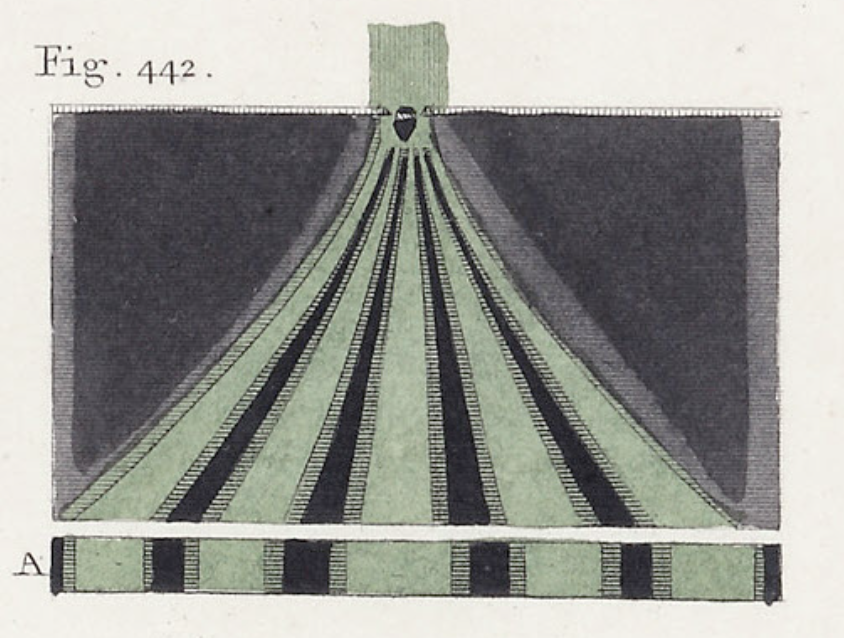
\includegraphics[width=0.5\linewidth,height=\textheight,keepaspectratio]{wave-optics/img/youngs_exp.png}

}

\caption{Young's double-slit experiment}

\end{figure}%

\textbf{1818: Augustin-Jean Fresnel} - Developed comprehensive
mathematical theory of diffraction. - Explained polarization through
transverse waves. - Created Fresnel equations for reflection and
refraction.

\end{tcolorbox}

Wave optics extends our understanding beyond the limitations of
geometric optics by treating light as a wave phenomenon. This approach
explains effects that cannot be accounted for by ray tracing alone, such
as:

\begin{itemize}
\tightlist
\item
  Interference (the combination of waves)
\item
  Diffraction (the bending of waves around obstacles or through
  apertures)
\item
  Color (the wavelength-dependent nature of light)
\end{itemize}

Light is part of the electromagnetic spectrum, which spans an enormous
range of frequencies. The visible region, extending approximately from
400 nm (violet) to 700 nm (red), represents only a small fraction of
this spectrum. This wave description is essential for understanding many
optical phenomena that geometric optics cannot explain, particularly
when dealing with structures comparable in size to the wavelength of
light.

\begin{figure}

\centering{

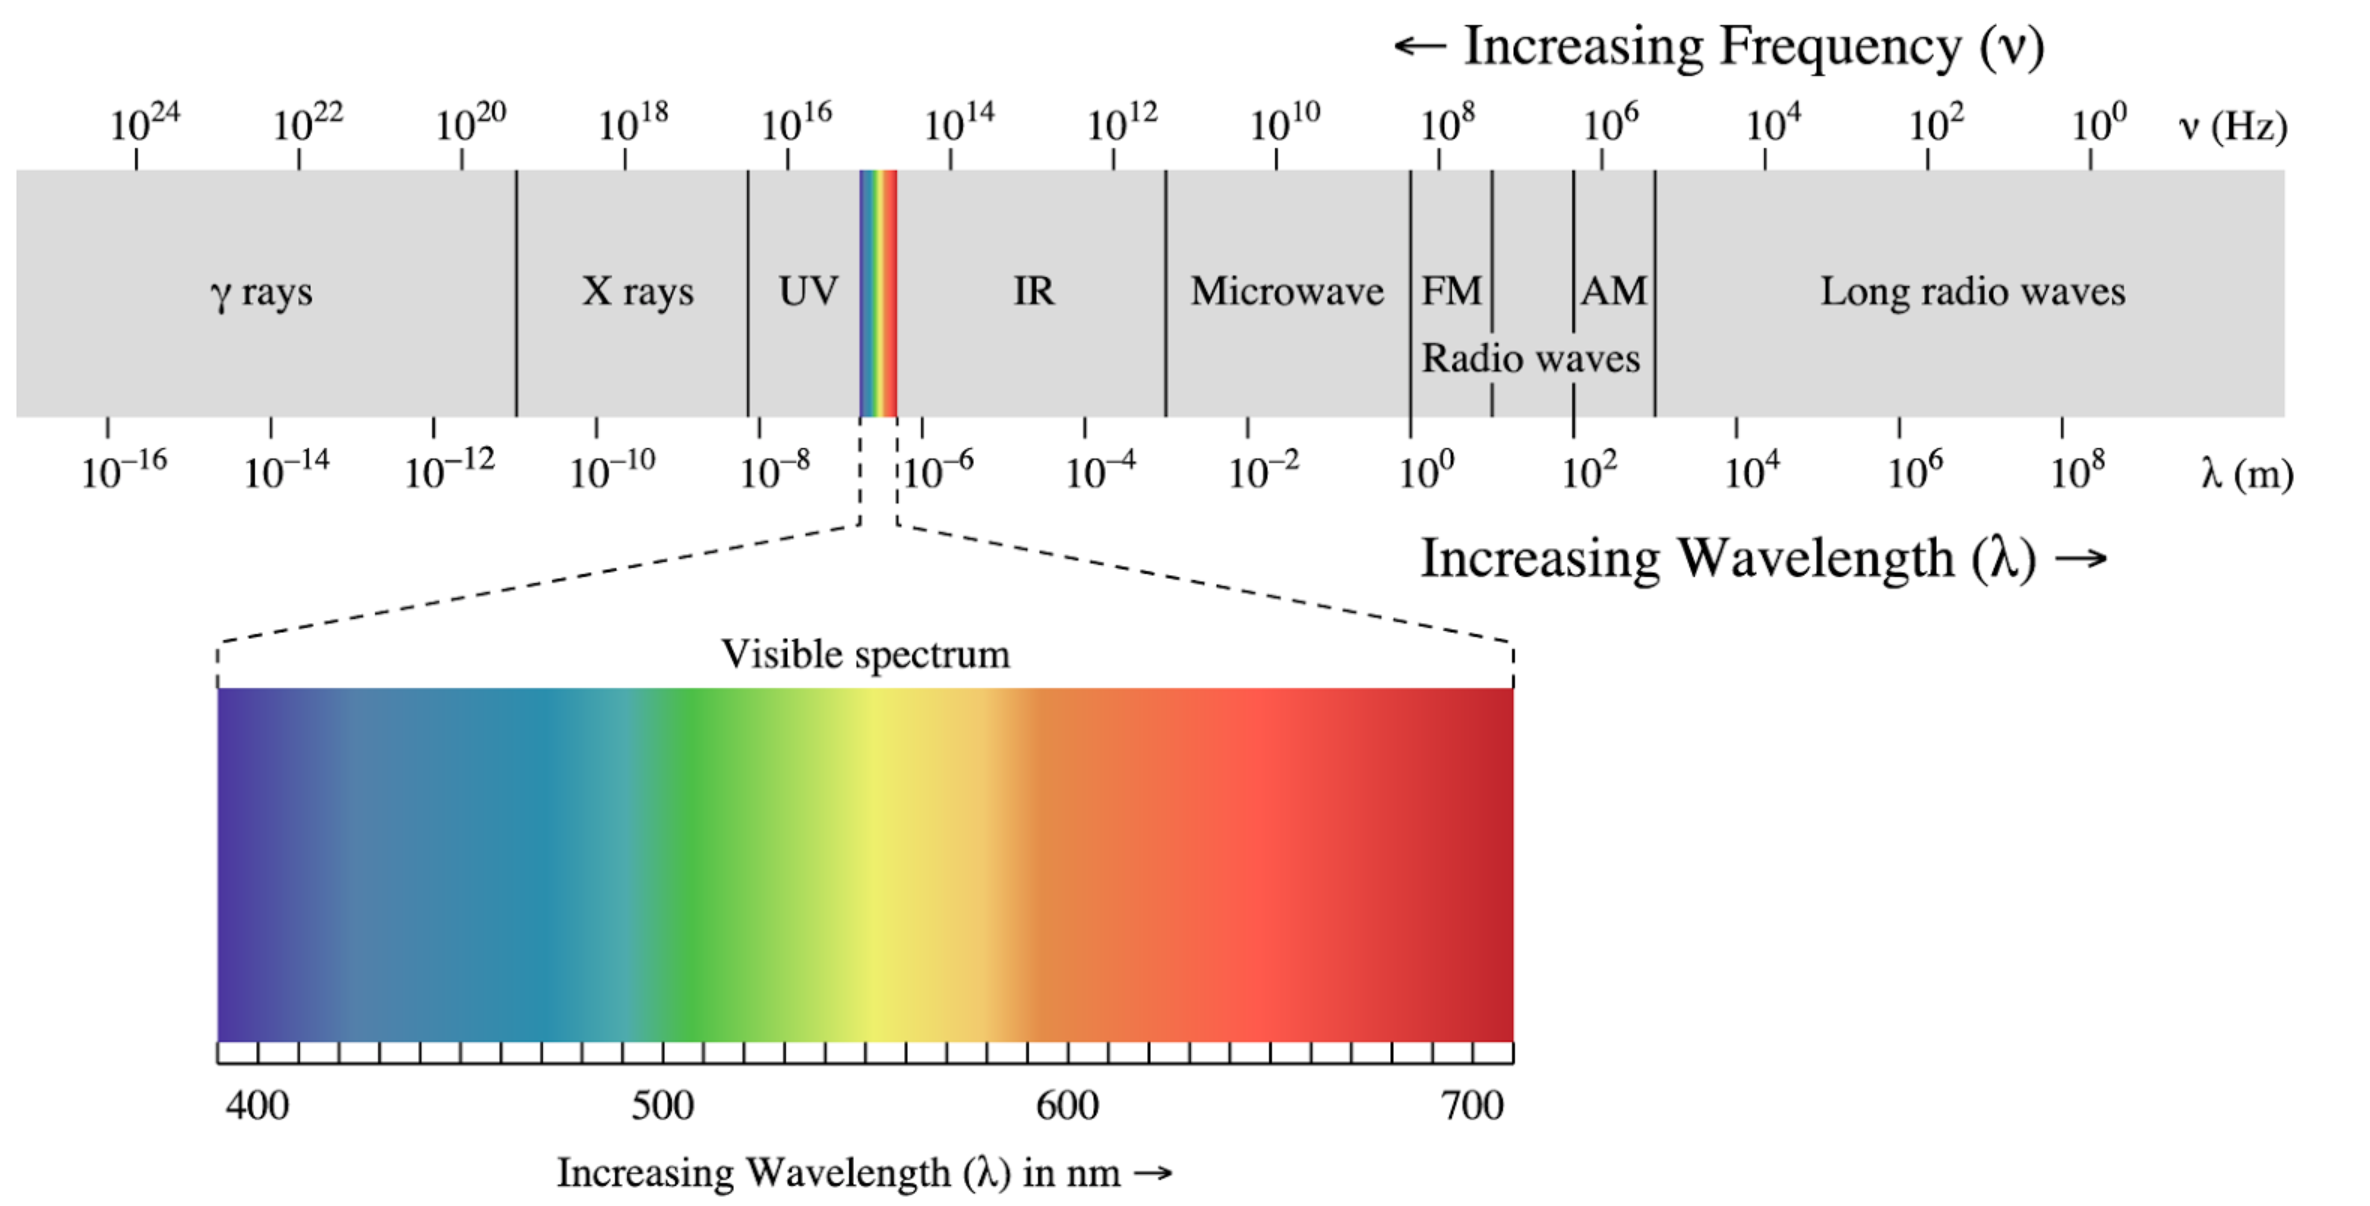
\includegraphics[width=0.7\linewidth,height=\textheight,keepaspectratio]{wave-optics/img/spectrum.png}

}

\caption{\label{fig-spectrum}Electromagnetic Spectrum with its different
regions}

\end{figure}%

In the following, we would like to introduce wave by discarding the
fact, that light is related to electric and magnetic fields. This is
useful as the vectorial nature of the electric and magnetic field
further complicates the calculations, but we do not need those yet.
Accordingly we also do not understand how light really interacts with
matter and we therefore have to introduce some postulates as well.

\section{Postulates of Wave Optics}\label{postulates-of-wave-optics}

\begin{tcolorbox}[enhanced jigsaw, breakable, toptitle=1mm, bottomrule=.15mm, colbacktitle=quarto-callout-note-color!10!white, title=\textcolor{quarto-callout-note-color}{\faInfo}\hspace{0.5em}{Wave}, arc=.35mm, rightrule=.15mm, bottomtitle=1mm, opacityback=0, toprule=.15mm, coltitle=black, leftrule=.75mm, opacitybacktitle=0.6, colback=white, left=2mm, titlerule=0mm, colframe=quarto-callout-note-color-frame]

A wave corresponds to a physical quantity which oscillates in space and
time. Its energy current density is related to the square magnitude of
the amplitude.

\end{tcolorbox}

\subsection{Wave equation}\label{wave-equation}

\[
\nabla^2 u - \frac{1}{c^2}\frac{\partial^2 u}{\partial t^2}=0
\]

where the Laplace operator \(\nabla^2\) is defined as:

\[
\nabla^2 =\frac{\partial^2}{\partial x^2}+\frac{\partial^2}{\partial y^2}+\frac{\partial^2}{\partial z^2}
\]

The wave equation is a linear differential equation, which implies that
the superposition principle holds. Specifically, if
\(u_1(\mathbf{r},t)\) and \(u_2(\mathbf{r},t)\) are solutions of the
wave equation, then any linear combination:

\[
u(\mathbf{r},t)=a_1u_1(\mathbf{r},t)+a_2u_2(\mathbf{r},t)
\]

is also a solution, where \(a_1\) and \(a_2\) are arbitrary constants.

\subsection{Monochromatic Wave}\label{monochromatic-wave}

A monochromatic wave consists of a single frequency \(\omega\). By
definition, such a wave must be infinite in time and free from phase
disturbances (such as sudden jumps). The mathematical expression for a
monochromatic wave is:

\[u(\mathbf{r},t)=a(\mathbf{r})\cos(\omega t + \phi(\mathbf{r}))\]

where:

\begin{itemize}
\tightlist
\item
  \(a(\mathbf{r})\) represents the amplitude
\item
  \(\phi(\mathbf{r})\) represents the spatial phase
\item
  \(\omega\) represents the angular frequency
\end{itemize}

\begin{figure}

\centering{

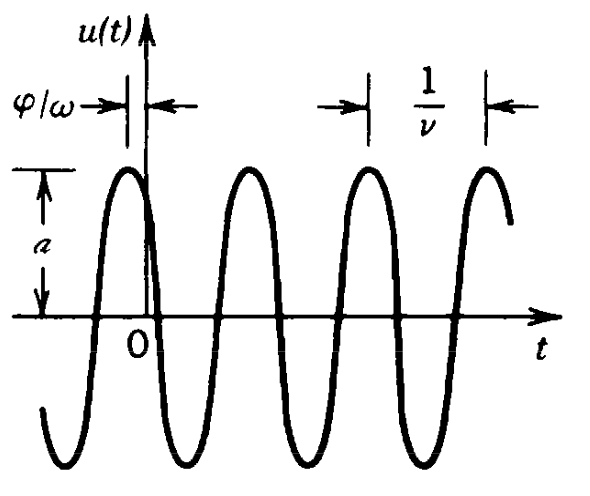
\includegraphics[width=0.5\linewidth,height=\textheight,keepaspectratio]{wave-optics/img/wave.png}

}

\caption{\label{fig-wave}Representation of a wavefunction over time
(constant position) denoting the phase \(\phi\) and the period
\(T=1/\nu\)}

\end{figure}%

\subsubsection{Complex Amplitude}\label{complex-amplitude}

The wave can be represented in complex form as:

\[
U(\mathbf{r},t)=a(\mathbf{r})e^{i\phi(\mathbf{r})}e^{i\omega t}
\]

This is known as the complex wavefunction.

\begin{figure}

\centering{

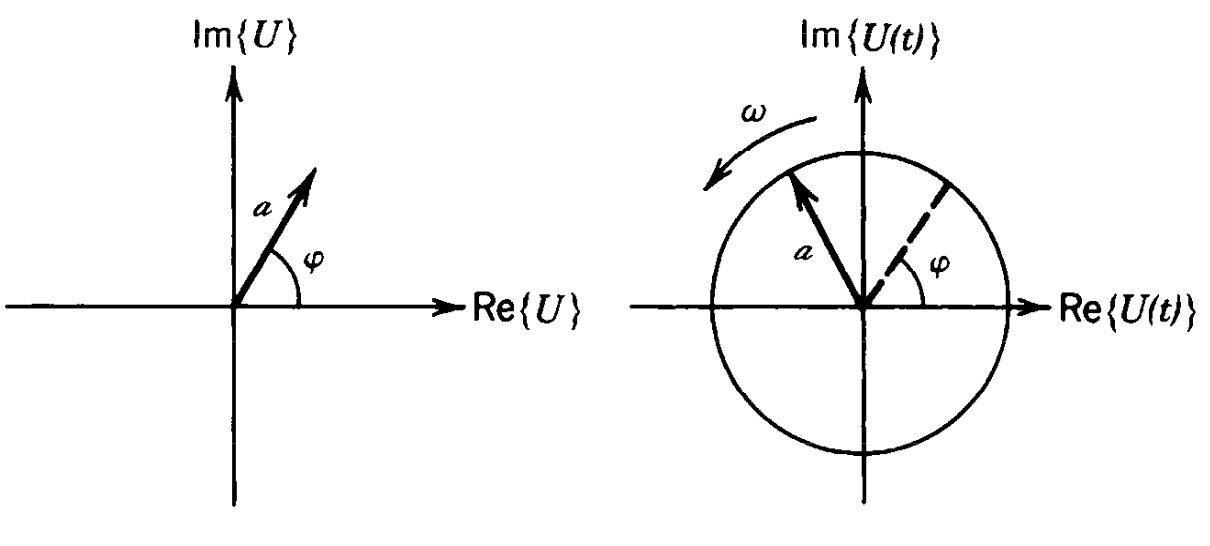
\includegraphics[width=0.7\linewidth,height=\textheight,keepaspectratio]{wave-optics/img/complex_rep.png}

}

\caption{\label{fig-complex-rep}Phasor diagram of the complex amplitude
\(U(\mathbf{r})\) (left) and \(U(t)\) (right)}

\end{figure}%

\begin{tcolorbox}[enhanced jigsaw, breakable, toptitle=1mm, bottomrule=.15mm, colbacktitle=quarto-callout-note-color!10!white, title=\textcolor{quarto-callout-note-color}{\faInfo}\hspace{0.5em}{Note}, arc=.35mm, rightrule=.15mm, bottomtitle=1mm, opacityback=0, toprule=.15mm, coltitle=black, leftrule=.75mm, opacitybacktitle=0.6, colback=white, left=2mm, titlerule=0mm, colframe=quarto-callout-note-color-frame]

A phasor displays the complex amplitude with magnitude and phase as a
vector in the complex plane.

\end{tcolorbox}

The relationship between the complex and real wavefunctions is:

\[
u(\mathbf{r},t)=\text{Re}\{U(\mathbf{r},t)\}=\frac{1}{2}[U(\mathbf{r},t)+U^*(\mathbf{r},t)]
\]

The complex wavefunction satisfies the same wave equation:

\[
\nabla^2 U - \frac{1}{c^2}\frac{\partial^2 U}{\partial t^2}=0
\]

We can separate the complex wavefunction into spatial and temporal
components:

\[
U(\mathbf{r},t)=U(\mathbf{r})e^{i\omega t}
\]

where

\[
U(\mathbf{r})=a(\mathbf{r})e^{i\phi(\mathbf{r})}
\]

Here, \(\phi\) represents the spatial phase of the wavefunction.
Substituting this into the wave equation and noting that the time
derivatives bring down factors of \(i\omega\):

\[\nabla^2 [U(\mathbf{r})e^{i\omega t}] - \frac{1}{c^2}\frac{\partial^2}{\partial t^2}[U(\mathbf{r})e^{i\omega t}] = 0\]
\[\nabla^2 U(\mathbf{r})e^{i\omega t} + \frac{\omega^2}{c^2}U(\mathbf{r})e^{i\omega t} = 0\]

The time dependence \(e^{i\omega t}\) factors out, leaving us with
\textbf{the Helmholtz equation}:

\[\nabla^2 U(\mathbf{r}) + k^2U(\mathbf{r}) = 0\]

where \(k = \omega/c\) is the wave number. This equation describes the
spatial behavior of monochromatic waves.

\subsubsection{Intensity of Waves}\label{intensity-of-waves}

The intensity of a wave at position \(\mathbf{r}\) and time \(t\) is
defined as:

\[
I(\mathbf{r},t)=2\langle u^2(\mathbf{r},t)\rangle
\]

where \(I\) is measured in units of \(\left[\frac{W}{m^2}\right]\). The
angle brackets \(\langle \ldots \rangle\) represent a time average over
one oscillation cycle of \(u\). For visible light, this averaging occurs
over an extremely brief period - for example, light with a wavelength of
600 nm has a cycle duration of just 2 femtoseconds.

The optical power \(P\) of a wave can be calculated by integrating the
intensity over a surface area \(A\):

\[
P=\int_A I(\mathbf{r},t) \, dA
\]

Inserting the seperation of the complex wavefunction into spatial and
temporal components leads to the following expression for the intensity:

\[
I(\mathbf{r})=|U(\mathbf{r})|^2
\]

Thus the physical quantity forming the spatial and temporal oscillation
of the wavefunction is also providing the intensity of the wave when its
magnitude is squared. This is a fundamental property of wavefunctions
and for example not the case when temperature oscillates in space and
time in a medium.

\subsubsection{Wavefronts}\label{wavefronts}

Wavefronts are surfaces in space where the phase is constant:

\[
\phi(\mathbf{r})=\text{const}
\]

Typically, this constant is chosen to represent points of maximum
spatial amplitude, such that:

\[
\phi(\mathbf{r})=2\pi q
\]

where \(q\) is an integer.

The direction normal to these wavefronts can be described by the
gradient vector:

\[
\mathbf{n}=\nabla\phi=\left(\frac{\partial \phi}{\partial x},\frac{\partial \phi}{\partial y},\frac{\partial \phi}{\partial z}\right)
\]

This vector \(\mathbf{n}\) is always perpendicular to the wavefront
surface and points in the direction of wave propagation. The evolution
of these wavefronts in time provides important information about the
wave's propagation characteristics.

\section{Plane Waves}\label{plane-waves}

A plane wave represents a fundamental solution of the homogeneous wave
equation. In its complex form, it is expressed as:

\begin{equation}
U(\mathbf{r},t)=Ae^{-i\mathbf{k}\cdot \mathbf{r}}e^{i\omega t}
\end{equation}

where:

\begin{itemize}
\tightlist
\item
  The first exponential term contains the spatial phase
\item
  The second exponential term contains the temporal phase
\item
  \(A\) is the (potentially complex) amplitude of the plane wave
\end{itemize}

The wavefront of a plane wave is defined by:

\[\mathbf{k}\cdot \mathbf{r}=2\pi q + \text{arg}(A)\]

where \(1\) is an integer. It just means that the projection of the
position vector \(\mathbf{r}\) onto the wavevector \(\mathbf{k}\) is a
multiple of \(2\pi\). This equation describes a plane perpendicular to
the wavevector \(\mathbf{k}\). Adjacent wavefronts are separated by the
wavelength \(\lambda=2\pi/k\), where \(k\) represents the spatial
frequency of the wave oscillation.

The spatial component of the plane wave is given by:

\begin{equation}
U(\mathbf{r})=Ae^{-i\mathbf{k}\cdot \mathbf{r}}
\end{equation}

In vacuum, the wavevector \(\mathbf{k}=\mathbf{k}_0\) is real-valued and
can be written as:

\begin{equation}
\mathbf{k}_0=
\begin{pmatrix}
k_{0x} \\
k_{0y}\\
k_{0z}\\
\end{pmatrix}
\end{equation}

\begin{figure}[H]

{\centering 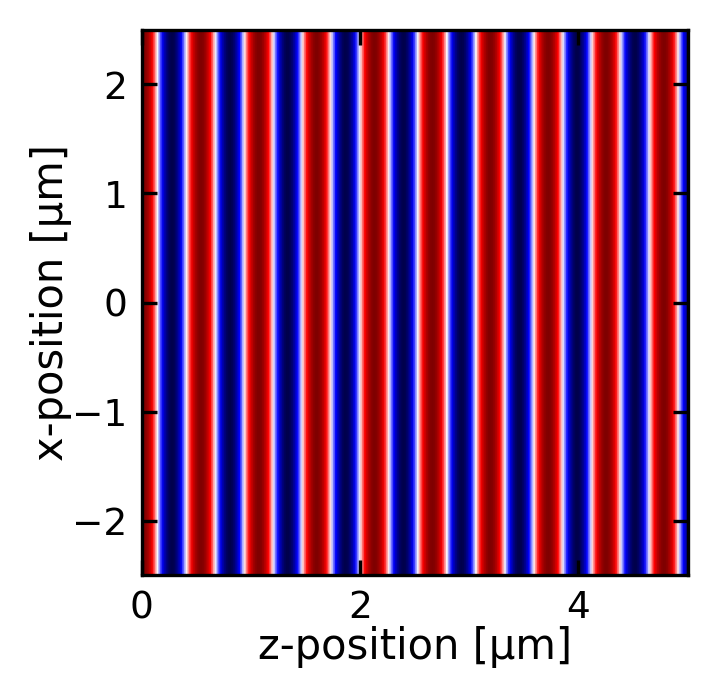
\includegraphics[width=3.72917in,height=3.63542in]{wave-optics/Wave Optics_files/figure-pdf/cell-3-output-1.png}

}

\caption{Plane wave}

\end{figure}%

\section{Dispersion Relation}\label{dispersion-relation}

Using the plane wave solution

\begin{equation}
U(\mathbf{r},t)=Ae^{-i\mathbf{k}\cdot \mathbf{r}}e^{i\omega t}
\end{equation}

we can write down the sum of the spatial and temporal phase as

\[
\phi(r,t)=\omega t-\mathbf{k}\cdot \mathbf{r}
\]

If we select a point on the wavefront \(\mathbf{r}_{m}\), and follow
that over time, the phase \(\phi(t)=\text{const}\). Taking the time
derivative results in

\[
\mathbf{k}\cdot \frac{d\mathbf{r}_{m}}{dt}=\omega
\]

If we choose the direction of the wavevector for measuring the
propagation speed, i.e.~\(\mathbf{r}_{m}=r_{m}\mathbf{e}_k\) then we
find for the propagation speed

\[
\frac{dr_{m}}{dt}=\frac{\omega}{k}
\]

or in vacuum

\begin{equation}
c_0=\frac{\omega}{k_0}
\end{equation}

This fundamental relationship connects:

\begin{itemize}
\tightlist
\item
  The momentum (\(k\)),
\item
  The energy (\(\omega\))
\end{itemize}

and is called a dispersion relation despite the fact, that we do not
really understand why those quantities are related to energy and
momentum.

\begin{tcolorbox}[enhanced jigsaw, breakable, toptitle=1mm, bottomrule=.15mm, colbacktitle=quarto-callout-note-color!10!white, title=\textcolor{quarto-callout-note-color}{\faInfo}\hspace{0.5em}{Note}, arc=.35mm, rightrule=.15mm, bottomtitle=1mm, opacityback=0, toprule=.15mm, coltitle=black, leftrule=.75mm, opacitybacktitle=0.6, colback=white, left=2mm, titlerule=0mm, colframe=quarto-callout-note-color-frame]

Light in free space exhibits a linear dispersion relation, i.e.~the
frequency of light changes linearly with the wavevector magnitude.

\end{tcolorbox}

Note that if we choose a different propagation direction \(\mathbf{e}\)
than the one along the wavevector \(\mathbf{e}_k\), we can write the
phase velocity as

\[
\mathbf{k}\cdot\mathbf{e} \frac{dr}{dt}=k\cos(\measuredangle\mathbf{k},\mathbf{e}) \frac{dr}{dt}=\omega
\]

or

\[
\frac{dr}{dt}=\frac{\omega}{k\cos(\measuredangle\mathbf{k},\mathbf{e})}
\]

which means that if you observe the wavepropagation not in the direction
of the wavevector, the phase velocity is actually bigger than the speed
of light and even tends to infinity if the angle between the wavevector
and the observation direction tends to 90°.

\section{Propagation in a Medium}\label{propagation-in-a-medium}

When a wave propagates through a medium:

\begin{enumerate}
\def\labelenumi{\arabic{enumi}.}
\tightlist
\item
  The frequency \(\omega\) remains constant (determined by the source)
\item
  The wave speed changes according to: \[
  c=\frac{c_0}{n}
  \] where \(n\) is the refractive index of the medium
\end{enumerate}

This leads to changes in:

\begin{itemize}
\item
  the wavelength, which becomes shorter in the medium \[
  \lambda=\frac{\lambda_0}{n}
  \]
\item
  the length of the wavevector, which increases in the medium \[
  k=nk_0
  \]
\end{itemize}

\section{Snells Law}\label{snells-law-1}

The change in the length of the wavevector has some simple consequence
for Snells law. We can write Snells law as

\[
n_1k_0\sin(\theta_1)=n_2k_0\sin(\theta_2)
\]

where \(k_0\) is the wavevector length in vacuum. As the \(n_1k_0\) is
the magnitude of the wavevector in medium 1, and \(n_2k_0\) is the
magnitude of the wavevector in medium 2, we can rewrite Snells law as

\[
k_1\sin(\theta_1)=k_2\sin(\theta_2)
\]

which means that the component of the wavevector parallel to the
interface is conserved. If the wavevector has constant length then the
wavevector incident at different angles is between a point on a circle
and the origin in the diagram below. The circle corresponds to an
isofrequency surface.

\begin{figure}

\begin{minipage}{0.33\linewidth}

\begin{figure}[H]

{\centering 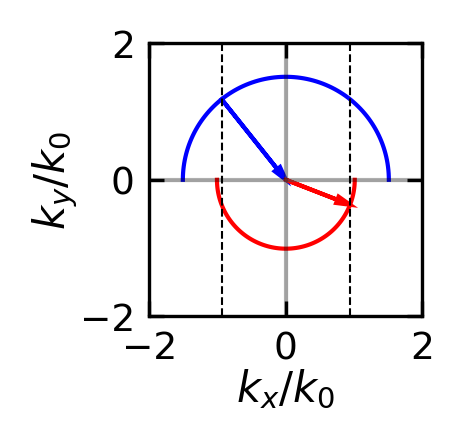
\includegraphics[width=2.41667in,height=2.29167in]{wave-optics/Wave Optics_files/figure-pdf/cell-4-output-1.png}

}

\subcaption{Snells law construction using the conservation of the
wavevector component parallel to the interface. The vertical dashed
lines indicate the parallal component of the wavevector in the two
media.}

\end{figure}%

\end{minipage}%
%
\begin{minipage}{0.33\linewidth}

\begin{figure}[H]

{\centering 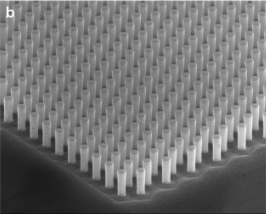
\includegraphics[width=0.9\linewidth,height=\textheight,keepaspectratio]{wave-optics/img/pc_ex.png}

}

\subcaption{Electron microscopy image of a 2D photonic crystal}

\end{figure}%

\end{minipage}%
%
\begin{minipage}{0.33\linewidth}

\begin{figure}[H]

{\centering 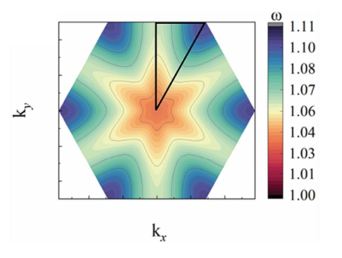
\includegraphics[width=1\linewidth,height=\textheight,keepaspectratio]{wave-optics/img/pc_iso.png}

}

\subcaption{Isofrequency surfaces of a photonic crystal}

\end{figure}%

\end{minipage}%

\end{figure}%

Isofrequency surfaces can have non-spherical shape. In anisotropic
media, they can be ellipsoids. In photonic crystals, i.e.~crystals with
a periodic structure on the scale of the wavelength, they can have a
more complex shape.

\section{Spherical Waves}\label{spherical-waves}

A spherical wave, like a plane wave, consists of spatial and temporal
components, but with wavefronts forming spherical surfaces. For
spherical waves, \(|\mathbf{k}||\mathbf{r}|=kr=\text{const}\). Given a
source at position \(\mathbf{r}_0\), the spherical wave can be expressed
as:

\begin{equation}
U=\frac{A}{|\mathbf{r}-\mathbf{r}_0|}e^{-ik|\mathbf{r}-\mathbf{r}_0|} e^{i\omega t}
\end{equation}

\begin{tcolorbox}[enhanced jigsaw, breakable, toptitle=1mm, bottomrule=.15mm, colbacktitle=quarto-callout-important-color!10!white, title=\textcolor{quarto-callout-important-color}{\faExclamation}\hspace{0.5em}{Important}, arc=.35mm, rightrule=.15mm, bottomtitle=1mm, opacityback=0, toprule=.15mm, coltitle=black, leftrule=.75mm, opacitybacktitle=0.6, colback=white, left=2mm, titlerule=0mm, colframe=quarto-callout-important-color-frame]

The \(1/|\mathbf{r}-\mathbf{r}_0|\) factor in the amplitude is necessary
for energy conservation - ensuring that the total energy flux through
any spherical surface centered on the source remains constant.

\end{tcolorbox}

\begin{figure}[H]

{\centering 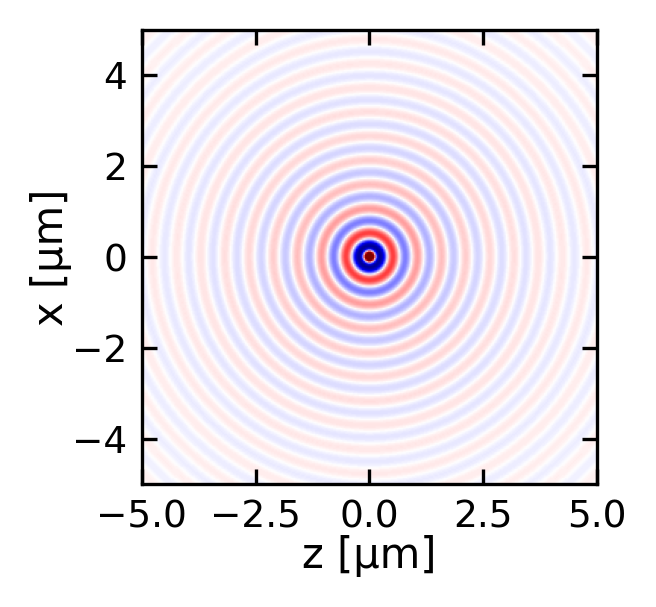
\includegraphics[width=3.41667in,height=3.15625in]{wave-optics/Wave Optics_files/figure-pdf/cell-5-output-1.png}

}

\caption{Spherical wave propagation. The wave is emitted from the origin
and propagates in the positive z-direction. The wavefronts are spherical
surfaces. The wave is visualized in the xz-plane.}

\end{figure}%

\begin{figure}

\centering{

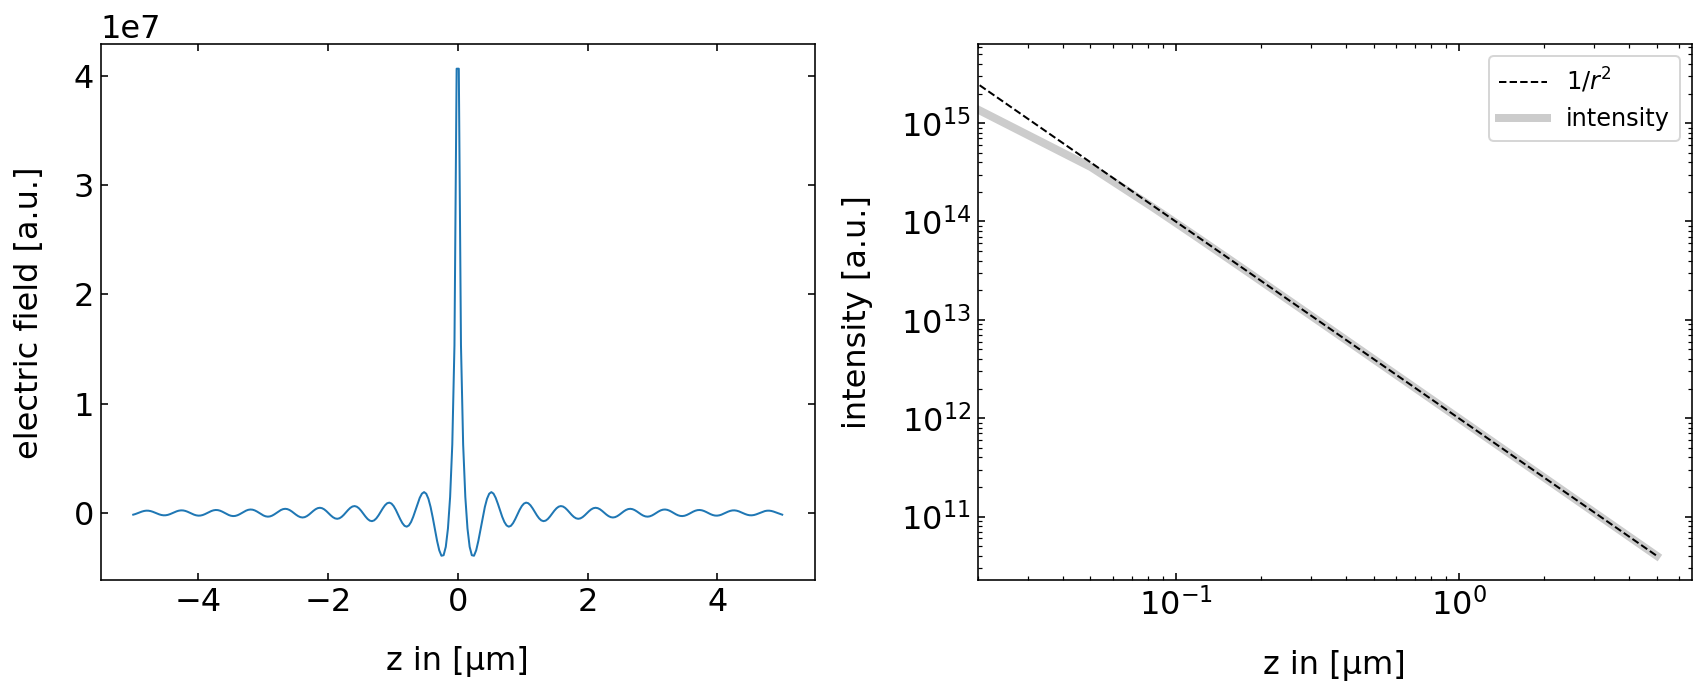
\includegraphics[width=1\linewidth,height=\textheight,keepaspectratio]{wave-optics/img/spherical_wave.png}

}

\caption{\label{fig-spherical-amplitude}Spherical wave amplitude and
intensity of the spherical wave as a function of distance from the
source}

\end{figure}%

The plots demonstrate that:

\begin{itemize}
\tightlist
\item
  The field amplitude decays rapidly with distance
\item
  The intensity follows a \(1/r^2\) law (with slight deviations at small
  distances due to discretization artifacts)
\end{itemize}

Note: The direction of wave propagation can be reversed by changing the
sign of the wavenumber \(k\).

\chapter{Interference}\label{interference}

Interference is a fundamental physical phenomenon that demonstrates the
superposition principle for linear systems. This principle, which states
that the net response to multiple stimuli is the sum of the individual
responses, is central to our understanding of wave physics. Interference
appears across many domains of physics: in optics where it enables
high-precision measurements and holography, in quantum mechanics where
it reveals the wave nature of matter, and in acoustics where it forms
the basis for noise cancellation technology. The ability of waves to
interfere constructively (amplifying each other) or destructively
(canceling each other) has profound practical applications, from the
anti-reflective coatings on optical elements to the operational
principles of interferometric gravitational wave detectors like LIGO.
Understanding interference is therefore not just of theoretical interest
but crucial for modern technology and experimental physics.

When two wave solutions \(U_1(\mathbf{r})\) and \(U_2(\mathbf{r})\)
combine, their superposition gives:

\[
U(\mathbf{r})=U_1(\mathbf{r})+U_2(\mathbf{r})
\]

The resulting intensity is:

\begin{eqnarray}
I &= &|U|^2\\
&= &|U_1+U_2|^2\\
&= &|U_1|^2+|U_2|^2+U^{*}_1 U_2 + U_1 U^{*}_2
\end{eqnarray}

The individual wave intensities are given by \(I_1=|U_1|^2\) and
\(I_2=|U_2|^2\). Using this, we can express each complex wave amplitude
in polar form, separating its magnitude (related to intensity) and
phase:

\[
U_1=\sqrt{I_1}e^{i\phi_1}
\] \[
U_2=\sqrt{I_2}e^{i\phi_2}
\]

Substituting these expressions back into our interference equation and
performing the algebra, the total intensity becomes:

\[
I=I_1+I_2+2\sqrt{I_1 I_2}\cos(\Delta \phi)
\]

where \(\Delta \phi=\phi_2-\phi_1\) is the phase difference between the
waves. This equation is known as the interference formula and contains
three terms:

\begin{itemize}
\tightlist
\item
  \(I_1\) and \(I_2\): the individual intensities
\item
  \(2\sqrt{I_1 I_2}\cos(\Delta \phi)\): the interference term that can
  be positive or negative
\end{itemize}

A particularly important special case occurs when the interfering waves
have equal intensities (\(I_1=I_2=I_0\)). The equation then simplifies
to:

\[
I=2I_0(1+\cos(\Delta \phi))=4I_0\cos^2\left(\frac{\Delta \phi}{2}\right)
\]

This last form clearly shows that:

\begin{itemize}
\tightlist
\item
  Maximum intensity (\(4I_0\)) occurs when \(\Delta \phi = 2\pi n\)
  (constructive interference)
\item
  Zero intensity occurs when \(\Delta \phi = (2n+1)\pi\) (destructive
  interference)
\item
  The intensity varies sinusoidally with the phase difference
\end{itemize}

\begin{tcolorbox}[enhanced jigsaw, breakable, toptitle=1mm, bottomrule=.15mm, colbacktitle=quarto-callout-note-color!10!white, title=\textcolor{quarto-callout-note-color}{\faInfo}\hspace{0.5em}{Constructive Interference}, arc=.35mm, rightrule=.15mm, bottomtitle=1mm, opacityback=0, toprule=.15mm, coltitle=black, leftrule=.75mm, opacitybacktitle=0.6, colback=white, left=2mm, titlerule=0mm, colframe=quarto-callout-note-color-frame]

Occurs when \(\Delta \phi=2\pi m\) (where \(m\) is an integer),
resulting in \(I=4I_0\)

\end{tcolorbox}

\begin{figure}[H]

{\centering \pandocbounded{
\includegraphics[keepaspectratio]{wave-optics/Interference_files/figure-pdf/cell-3-output-1.pdf}}

}

\caption{Constructive interference of two waves (top, middle) and the
sum of the two wave amplitudes (bottom)}

\end{figure}%

\begin{tcolorbox}[enhanced jigsaw, breakable, toptitle=1mm, bottomrule=.15mm, colbacktitle=quarto-callout-note-color!10!white, title=\textcolor{quarto-callout-note-color}{\faInfo}\hspace{0.5em}{Destructive Interference}, arc=.35mm, rightrule=.15mm, bottomtitle=1mm, opacityback=0, toprule=.15mm, coltitle=black, leftrule=.75mm, opacitybacktitle=0.6, colback=white, left=2mm, titlerule=0mm, colframe=quarto-callout-note-color-frame]

Occurs when \(\Delta \phi=(2m-1)\pi\) (where \(m\) is an integer),
resulting in \(I=0\)

\end{tcolorbox}

\begin{figure}[H]

{\centering \pandocbounded{
\includegraphics[keepaspectratio]{wave-optics/Interference_files/figure-pdf/cell-4-output-1.pdf}}

}

\caption{Destructive interference of two waves (top, middle) and the sum
of the two wave amplitudes (bottom)}

\end{figure}%

\subsection{Phase and Path Difference}\label{phase-and-path-difference}

The phase difference \(\Delta \phi\) can be related to the path
difference \(\Delta s\) between the two waves. For two waves with the
same frequency \(\omega\), we can write their complete phase expressions
as:

\[\phi_1(\mathbf{r},t) = \mathbf{k}_1\cdot\mathbf{r} - \omega t + \phi_{01}\]
\[\phi_2(\mathbf{r},t) = \mathbf{k}_2\cdot\mathbf{r} - \omega t + \phi_{02}\]

where:

\begin{itemize}
\tightlist
\item
  \(\mathbf{k}_i\) are the wave vectors
\item
  \(\mathbf{r}\) is the position vector
\item
  \(\omega\) is the angular frequency
\item
  \(\phi_{0i}\) are initial phase constants
\end{itemize}

The instantaneous phase difference is then:

\[
\Delta\phi(\mathbf{r},t) = \phi_2(\mathbf{r},t) - \phi_1(\mathbf{r},t) = (\mathbf{k}_2-\mathbf{k}_1)\cdot\mathbf{r} + (\phi_{02}-\phi_{01})
\]

For stationary interference patterns, we typically observe the
time-independent phase difference. When the waves travel along similar
paths (same direction), this reduces to:

\[\Delta\phi = k\Delta s + \Delta\phi_0\]

where \(\Delta s\) is the path difference and \(\Delta\phi_0\) is any
initial phase difference between the sources.

\begin{tcolorbox}[enhanced jigsaw, breakable, toptitle=1mm, bottomrule=.15mm, colbacktitle=quarto-callout-important-color!10!white, title=\textcolor{quarto-callout-important-color}{\faExclamation}\hspace{0.5em}{Phase Difference and Path Difference}, arc=.35mm, rightrule=.15mm, bottomtitle=1mm, opacityback=0, toprule=.15mm, coltitle=black, leftrule=.75mm, opacitybacktitle=0.6, colback=white, left=2mm, titlerule=0mm, colframe=quarto-callout-important-color-frame]

A path difference \(\Delta s\) corresponds to a phase difference
\(k\Delta s=2\pi\Delta s/\lambda\). Path differences of integer
multiples of \(\lambda\) result in phase differences of integer
multiples of \(2\pi\).

\textbf{Important:} The path difference \(\Delta s\) represents the
\textbf{optical path difference}, not just the geometric distance. When
light travels through a medium with refractive index \(n\) over a
physical distance \(L\), the optical path length is
\(\text{OPL} = n \cdot L\). This distinction becomes crucial when
analyzing interferometers where light travels through different media or
when measuring refractive index changes.

\end{tcolorbox}

The principles of interference we've developed---relating phase
differences to path differences and understanding constructive and
destructive interference---form the foundation for a powerful class of
precision instruments called interferometers. These devices split light
into multiple paths, allow these paths to accumulate different optical
path lengths through either geometric differences or variations in
refractive index, and then recombine the beams to observe interference.
By carefully analyzing the resulting interference patterns,
interferometers can measure distances with sub-wavelength precision,
detect tiny changes in refractive index, and even sense gravitational
waves. We will explore these remarkable applications in detail in a
subsequent lecture on interferometers.

\subsection{Interference of Waves in
Space}\label{interference-of-waves-in-space}

\begin{figure}[H]

{\centering \pandocbounded{
\includegraphics[keepaspectratio]{wave-optics/Interference_files/figure-pdf/cell-5-output-1.pdf}}

}

\caption{Interference of two plane waves propagating under an angle of
45°. The two left graphs show the original waves. The two right show the
total amplitude and the intensity pattern.}

\end{figure}%

\begin{figure}[H]

{\centering \pandocbounded{
\includegraphics[keepaspectratio]{wave-optics/Interference_files/figure-pdf/cell-6-output-1.pdf}}

}

\caption{Interference of a spherical wave and a plane wave. The top
graphs show the original waves. The two bottom show the total amplitude
and the intensity pattern.}

\end{figure}%

The interference of the spherical and the plane wave (also the one of
the two plane waves) give also an interesting result. The intensity
resembles to be a snapshot of the shape of the wavefronts of the
spherical wave. We can therefore measure the wavefronts of the spherical
wave by interfering it with a plane wave. This is also the basic
principle behind holography. There we use a reference wave to interfere
with the wave that we want to measure. The interference pattern is
recorded and can be used to reconstruct the wavefronts of the wave.

A super nice website to try out interference interactively is
\href{https://www.falstad.com/ripple/}{here}.

\subsection{Coherence}\label{coherence}

In the earlier consideration we obtained a general description for the
phase difference between two waves. It is given by and contains the
optical path difference \(\Delta s\) and some intrinsic phase
\(\Delta\phi_0\) that could be part of the wave generation process.

\[\Delta\phi = k\Delta s + \Delta\phi_0\]

To observe stationary interference, it is important that these two
quantities are also stationary, i.e.~the phase relation between the two
waves is stationary. This relation between the phase of two waves is
called coherence and was assumed in all the examples before. Coherence
is particularly critical for interferometric applications: devices like
the Michelson interferometer, Fabry-Perot cavities, and other precision
instruments rely on highly coherent light sources (typically lasers) to
maintain stable interference patterns over the path length differences
involved in the measurements.

\begin{figure}[H]

{\centering 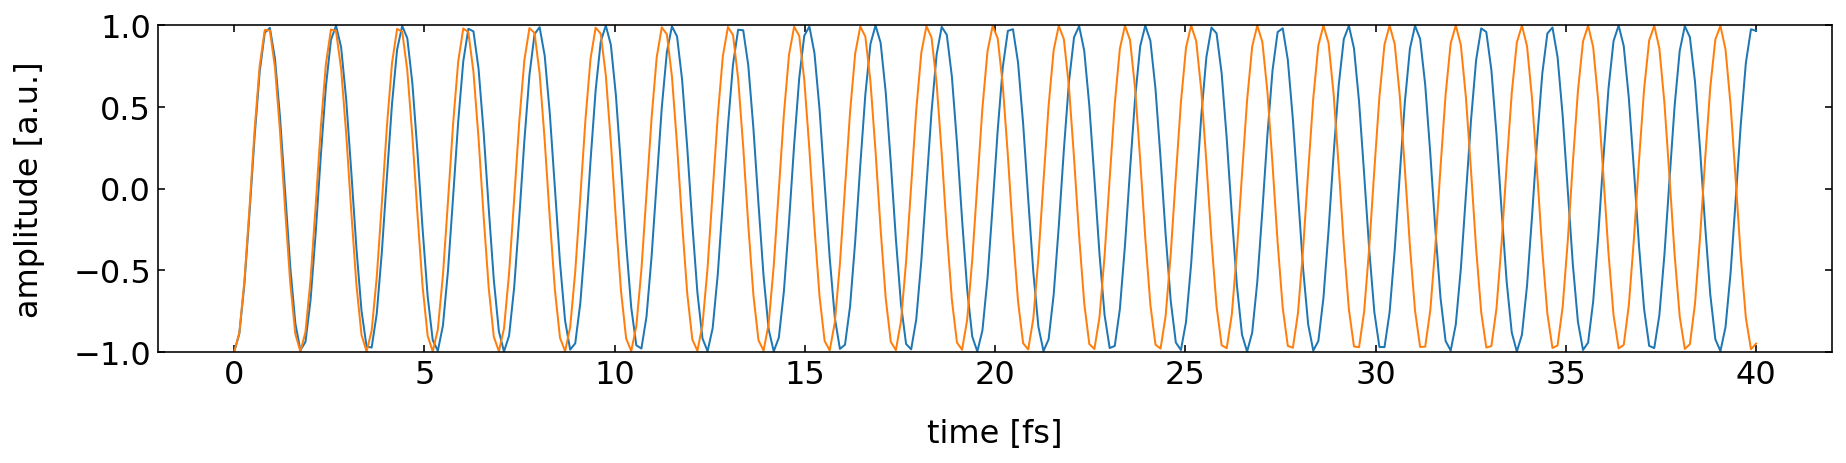
\includegraphics[width=0.9\linewidth,height=\textheight,keepaspectratio]{wave-optics/img/coherence.png}

}

\caption{Two waves of different frequency over time.}

\end{figure}%

The above image shows the timetrace of the amplitude of two wave with
slightly different frequency. Due to the frequency, the waves run out of
phase and have acquired a phase different of \(\pi\) after \(40\) fs.

The temporal coherence of two waves is now defined by the time it takes
for the two waves to obtain a phase difference of \(2\pi\). The phase
difference between two wave of frequency \(\nu_1\) and \(\nu_2\) is
given by

\[
\Delta \phi = 2\pi (\nu_2-\nu_1)(t-t_0)
\]

Here \(t_0\) refers to the time, when thw two waves were perfectly in
sync. Lets assume that the two frequencies are seperarated from a
central frequency \(\nu_0\) such that

\[
\nu_1=\nu_0-\Delta \nu/2
\] \[
\nu_2=\nu_0+\Delta \nu/2
\]

Inserting this into the first equation yields

\[
\Delta \phi = 2\pi \Delta \nu \Delta t
\]

with \(\Delta t=t-t_0\). We can now define the coherence time as the
time interval over which the phase shift \(\Delta \phi\) grows to
\(2\pi\), i.e.~\(\Delta \phi=2\pi\). The coherence time is thus

\[
\tau_{c}=\Delta t =\frac{1}{\Delta \nu}
\]

Thus the temporal coherence and the frequency distribution of the light
are intrisincly connected. Monochromatic light has \(\Delta nu=0\) and
thus the coherence time is infinitely long. Light with a wide spectrum
(white light for example) therefore has and extremly short coherence
time.

The coherence time is also connected to a coherence length. The
coherence length \(L_c\) is given by the distance light travels within
the coherence time \(\tau_c\), i.e.

\[
L_c=c\tau_c
\]

\begin{tcolorbox}[enhanced jigsaw, breakable, toptitle=1mm, bottomrule=.15mm, colbacktitle=quarto-callout-note-color!10!white, title=\textcolor{quarto-callout-note-color}{\faInfo}\hspace{0.5em}{Coherence}, arc=.35mm, rightrule=.15mm, bottomtitle=1mm, opacityback=0, toprule=.15mm, coltitle=black, leftrule=.75mm, opacitybacktitle=0.6, colback=white, left=2mm, titlerule=0mm, colframe=quarto-callout-note-color-frame]

Two waves are called coherent, if they exihibit a fixed phase relation
in space or time relation over time. It measures their ability to
interfer. The main types of coherence are

\subsection{Temporal Coherence}\label{temporal-coherence}

\begin{itemize}
\tightlist
\item
  Measures phase correlation of a wave with itself at different times
\item
  Characterized by coherence time \(\tau_c\) and coherence length
  \(L_c = c\tau_c\)
\item
  Related to spectral width: \(\tau_c = 1/\Delta\nu\)
\item
  Perfect for monochromatic waves (single frequency)
\item
  Limited for broad spectrum sources (like thermal light)
\end{itemize}

\subsection{Spatial Coherence}\label{spatial-coherence}

\begin{itemize}
\tightlist
\item
  Measures phase correlation between different points in space
\item
  Important for interference from extended sources
\item
  Determines ability to form interference patterns
\item
  Related to source size and geometry
\end{itemize}

Coherence is a property of the light source and is connected to the
frequency distribution of the light. Sources can be:

\begin{itemize}
\tightlist
\item
  \textbf{Fully coherent}: ideal laser
\item
  \textbf{Partially coherent}: real laser
\item
  \textbf{Incoherent}: thermal light
\end{itemize}

\end{tcolorbox}

\subsection{More General Description of
Coherence}\label{more-general-description-of-coherence}

While the above definition provides an intuitive picture based on
frequency spread, we can describe coherence more rigorously using
correlation functions. These functions measure how well a wave maintains
its phase relationships:

In real physical systems, perfect coherence (constant phase
relationship) between waves is rare. Partial coherence describes the
degree to which waves maintain a consistent phase relationship over time
and space. We can characterize this using correlation functions:

\begin{enumerate}
\def\labelenumi{\arabic{enumi}.}
\tightlist
\item
  \textbf{Temporal Coherence} The complex degree of temporal coherence
  is given by:
\end{enumerate}

\[g^{(1)}(\tau) = \frac{\langle U(t)U^*(t+\tau)\rangle}{\sqrt{\langle|U(t)|^2\rangle\langle|U(t+\tau)|^2\rangle}}\]

where:

\begin{itemize}
\tightlist
\item
  \(\tau\) is the time delay
\item
  \(U(t)\) is the electric field
\item
  \(\langle...\rangle\) denotes time averaging
\end{itemize}

\begin{enumerate}
\def\labelenumi{\arabic{enumi}.}
\setcounter{enumi}{1}
\tightlist
\item
  \textbf{Spatial Coherence} Similarly, spatial coherence between two
  points is characterized by:
\end{enumerate}

\[g^{(1)}(\mathbf{r}_1,\mathbf{r}_2) = \frac{\langle U(\mathbf{r}_1)U^*(\mathbf{r}_2)\rangle}{\sqrt{\langle|U(\mathbf{r}_1)|^2\rangle\langle|U(\mathbf{r}_2)|^2\rangle}}\]

The obtained correlation functions can be used to calculate the
coherence time and length and have the following properties:

\begin{itemize}
\tightlist
\item
  \(|g^{(1)}| = 1\) indicates perfect coherence
\item
  \(|g^{(1)}| = 0\) indicates complete incoherence
\item
  \(0 < |g^{(1)}| < 1\) indicates partial coherence
\end{itemize}

A finite coherence time and length is leads to partial coherence affects
interference visibility through:

\begin{itemize}
\tightlist
\item
  Reduced contrast in interference patterns
\item
  Limited coherence length/area
\item
  Spectral broadening
\end{itemize}

\begin{figure}[H]

{\centering \pandocbounded{
\includegraphics[keepaspectratio]{wave-optics/Interference_files/figure-pdf/cell-7-output-1.pdf}}

}

\caption{Temporal correlation for two waves with slightly different
frequencies. The vertical line indicates the coherence time τc = π/Δω.}

\end{figure}%

Besides different frequencies the coherence time can also be affected by
phase jumps. The following example shows two waves with the same
frequency but multiple phase jumps. The temporal correlation function
shows the decoherence due to the phase jumps.

\begin{figure}[H]

{\centering \pandocbounded{
\includegraphics[keepaspectratio]{wave-optics/Interference_files/figure-pdf/cell-8-output-1.pdf}}

}

\caption{Temporal correlation for two waves of same frequency showing
decoherence due to multiple phase jumps. Vertical lines indicate
positions of phase jumps.}

\end{figure}%

\begin{tcolorbox}[enhanced jigsaw, breakable, toptitle=1mm, bottomrule=.15mm, colbacktitle=quarto-callout-note-color!10!white, title=\textcolor{quarto-callout-note-color}{\faInfo}\hspace{0.5em}{Coherence of Thermal radiation}, arc=.35mm, rightrule=.15mm, bottomtitle=1mm, opacityback=0, toprule=.15mm, coltitle=black, leftrule=.75mm, opacitybacktitle=0.6, colback=white, left=2mm, titlerule=0mm, colframe=quarto-callout-note-color-frame]

Thermal radiation is a common example of incoherent light. While it is
called incoherent, there is no complete incoherence, but the coherence
length of a few 10 micrometers. Sun light, for example, has been
\href{https://www.semanticscholar.org/paper/Spatial-coherence-of-sunlight-and-its-implications-Divitt-Novotn\%C3\%BD/fbc2560b8fc54a10cb0feeac94eb3607e4e80ffb}{measured}
to have a coherence length of about 50 micrometers (Shawn Divitt and
Lukas Novotny, ``Spatial coherence of sunlight and its implications for
light management in photovoltaics,'' Optica 2, 95-103 (2015)). The
following factors contribute to the incoherence of thermal radiation:

\textbf{Random Emission Process} - Individual atoms/molecules emit light
independently - Each emission event has a random phase - The emission
timing is random - These random events effectively create continuous
phase jumps

\textbf{Multiple Emitters} - Many atoms/molecules emit simultaneously -
Each emitter acts independently - There's no phase relationship between
different emitters - This leads to spatially incoherent radiation

\textbf{Thermal Motion} - Atoms/molecules are in constant thermal motion
- This motion causes Doppler shifts - The shifts result in frequency
variations - Motion also affects the phase of emitted radiation

\textbf{Collision Effects} - Frequent atomic/molecular collisions - Each
collision can cause phase jumps - At higher temperatures, more frequent
collisions - This leads to shorter coherence times

\end{tcolorbox}

\begin{tcolorbox}[enhanced jigsaw, breakable, toptitle=1mm, bottomrule=.15mm, colbacktitle=quarto-callout-note-color!10!white, title=\textcolor{quarto-callout-note-color}{\faInfo}\hspace{0.5em}{Partial Coherence in Lasers}, arc=.35mm, rightrule=.15mm, bottomtitle=1mm, opacityback=0, toprule=.15mm, coltitle=black, leftrule=.75mm, opacitybacktitle=0.6, colback=white, left=2mm, titlerule=0mm, colframe=quarto-callout-note-color-frame]

The coherence of laser light is limited by various physical mechanisms
that cause fluctuations in phase and frequency. While perfect coherence
is theoretically impossible, some lasers can achieve remarkable
coherence lengths. Single-frequency solid-state lasers, when properly
stabilized, are particularly noteworthy in this regard. For instance, a
laser with a Lorentzian spectrum of 10 kHz linewidth can achieve a
coherence length of 9.5 km.

The fundamental limit to laser coherence is set by quantum noise, as
described by the Schawlow-Townes linewidth. However, modern laser
systems, particularly those developed for optical clocks, have pushed
these boundaries further. Some of these systems have been stabilized to
achieve linewidths below one hertz, corresponding to coherence lengths
exceeding 300,000 km.

\textbf{Spontaneous Emission} - Not all emission in a laser is
stimulated - Some spontaneous emission is always present - Adds random
phase jumps to the laser field - Sets fundamental quantum limit to
coherence

\textbf{Technical Noise Sources} - Mechanical vibrations of cavity
mirrors - Thermal fluctuations in gain medium - Pump power fluctuations
- Current noise in diode lasers

\textbf{Gain Medium Properties} - Finite linewidth of the lasing
transition - Thermal motion of atoms/molecules - Pressure broadening in
gas lasers - Population fluctuations

\textbf{Cavity Effects} - Finite cavity lifetime - Multiple longitudinal
modes - Temperature-induced length changes

\end{tcolorbox}

\chapter{Double Slit Interference}\label{double-slit-interference}

The double slit experiment stands as one of the most elegant and
profound demonstrations in all of physics. First performed by Thomas
Young in 1801, this experiment provided compelling evidence for the wave
nature of light, challenging the prevailing corpuscular theory
championed by Newton. Young's observation of interference
fringes---alternating bright and dark bands on a screen---could only be
explained if light behaved as a wave, capable of interfering
constructively and destructively. This single experiment fundamentally
changed our understanding of light and laid the groundwork for wave
optics.

Beyond its historical significance, the double slit experiment reveals
principles that are essential for modern technology. The same physics
governs how we design diffraction gratings for spectroscopy, how we
understand the resolution limits of microscopes and telescopes, and how
we engineer photonic devices for telecommunications. Even more
remarkably, the double slit experiment continues to surprise us in
quantum mechanics, where individual photons or electrons create
interference patterns that challenge our intuitions about the nature of
reality itself.

\section{Two Point Sources: The Foundation of Double Slit
Interference}\label{two-point-sources-the-foundation-of-double-slit-interference}

The interference pattern we observe in the double slit experiment arises
from the superposition of waves emanating from two coherent point
sources. We can model the double slit as two such sources separated by a
distance \(d\), each emitting spherical waves with the same wavelength
\(\lambda\) and amplitude. When these waves overlap in space, they
interfere according to the principle of superposition, creating regions
of constructive interference (bright fringes) where the waves arrive in
phase, and regions of destructive interference (dark fringes) where they
arrive out of phase.

The key to understanding the interference pattern lies in calculating
the path difference between the two waves as they travel from the slits
to any point on an observation screen. This path difference determines
the relative phase of the waves at that point, which in turn determines
whether we observe constructive or destructive interference.

\begin{figure}

\begin{minipage}{0.50\linewidth}

\begin{figure}[H]

{\centering \pandocbounded{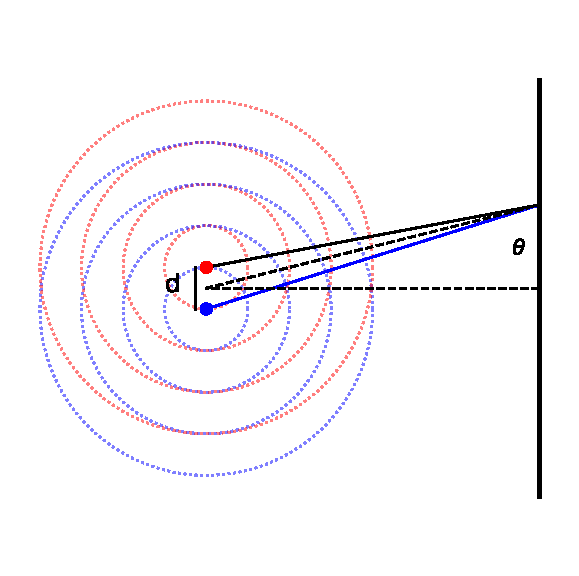
\includegraphics[keepaspectratio]{wave-optics/Double Slit_files/figure-pdf/cell-3-output-1.pdf}}

}

\subcaption{Double slit interference as the interference from two point
sources on the left and the wave amplitudes on the right. The
interference pattern is created by two point sources that emit waves
with the same wavelength and amplitude. The intereference of the two
waves depends then on the path length difference between the two waves.}

\end{figure}%

\end{minipage}%
%
\begin{minipage}{0.50\linewidth}

\end{minipage}%

\end{figure}%

\subsection{Calculating the Path Difference and Phase
Shift}\label{calculating-the-path-difference-and-phase-shift}

To understand where bright and dark fringes appear on the screen, we
need to calculate how the path difference between the two waves varies
with position. Consider light traveling from the two slits to a point on
a distant screen at angle \(\theta\) from the central axis. When the
screen is far away compared to the slit separation (the Fraunhofer or
far-field regime), we can approximate the two paths as nearly parallel
rays. In this approximation, the geometric path difference is simply the
projection of the slit separation onto the direction of propagation.

\begin{tcolorbox}[enhanced jigsaw, breakable, toptitle=1mm, bottomrule=.15mm, colbacktitle=quarto-callout-important-color!10!white, title=\textcolor{quarto-callout-important-color}{\faExclamation}\hspace{0.5em}{Path Difference and Phase Difference Formulas}, arc=.35mm, rightrule=.15mm, bottomtitle=1mm, opacityback=0, toprule=.15mm, coltitle=black, leftrule=.75mm, opacitybacktitle=0.6, colback=white, left=2mm, titlerule=0mm, colframe=quarto-callout-important-color-frame]

\textbf{Path difference:} \[\Delta s = d \sin(\theta)\]

\textbf{Phase difference:}
\[\Delta \phi = \frac{2\pi}{\lambda} \Delta s = \frac{2\pi d}{\lambda} \sin(\theta)\]

where:

\begin{itemize}
\tightlist
\item
  \(d\) = separation between the two slits
\item
  \(\theta\) = angle from the central axis to the observation point
\item
  \(\lambda\) = wavelength of light
\end{itemize}

\textbf{Physical meaning:} Light from the upper slit travels a distance
\(d\sin(\theta)\) farther than light from the lower slit. This extra
distance translates directly into a phase shift that determines the
interference pattern.

\end{tcolorbox}

The path difference formula \(\Delta s = d\sin(\theta)\) is fundamental
and remarkably simple, yet it encapsulates the entire geometry of the
double slit experiment. When \(\theta = 0\) (directly ahead, on the
central axis), both waves travel the same distance and arrive in phase,
creating the bright central maximum. As we move to larger angles, the
path difference increases, and the waves alternately come into and out
of phase, creating the characteristic fringe pattern.

\begin{tcolorbox}[enhanced jigsaw, breakable, toptitle=1mm, bottomrule=.15mm, colbacktitle=quarto-callout-note-color!10!white, title=\textcolor{quarto-callout-note-color}{\faInfo}\hspace{0.5em}{The Fraunhofer Approximation}, arc=.35mm, rightrule=.15mm, bottomtitle=1mm, opacityback=0, toprule=.15mm, coltitle=black, leftrule=.75mm, opacitybacktitle=0.6, colback=white, left=2mm, titlerule=0mm, colframe=quarto-callout-note-color-frame]

The path length difference formula \(\Delta s = d\sin(\theta)\) given
above is an approximation valid in the far-field or \textbf{Fraunhofer
limit}. The exact calculation requires careful geometry: for two sources
at positions \(z_1 = -d/2\) and \(z_2 = d/2\), and a point P at distance
\(L\) from the center with screen coordinate \(y_P\), the exact path
lengths are:

\[r_1 = \sqrt{L^2 + (y_P + d/2)^2}, \quad r_2 = \sqrt{L^2 + (y_P - d/2)^2}\]

The exact path difference is \(\Delta s = r_2 - r_1\). The approximation
\(\Delta s \approx d\sin(\theta)\) becomes accurate when the screen
distance \(L\) is much larger than both the slit separation \(d\) and
the observation height \(y_P\). Mathematically, we require \(L \gg d\)
and \(L \gg y_P\).

Interestingly, if we place a lens at one focal length from the screen
(as is commonly done in optical systems), the two paths become exactly
parallel rays, and our simple formula \(\Delta s = d\sin(\theta)\) is
exact rather than approximate. This is why many practical
interferometric setups use lenses to create well-defined far-field
patterns.

\end{tcolorbox}

\subsection{Conditions for Constructive and Destructive
Interference}\label{conditions-for-constructive-and-destructive-interference}

Armed with the phase difference formula, we can now determine where
bright and dark fringes appear. Constructive interference---where the
waves add coherently to create maximum intensity---occurs whenever the
phase difference is an integer multiple of \(2\pi\). This corresponds to
path differences that are integer multiples of the wavelength, meaning
the waves arrive perfectly in phase. Setting \(\Delta\phi = 2\pi m\)
where \(m\) is an integer, we obtain the condition for bright fringes.

\begin{tcolorbox}[enhanced jigsaw, breakable, toptitle=1mm, bottomrule=.15mm, colbacktitle=quarto-callout-important-color!10!white, title=\textcolor{quarto-callout-important-color}{\faExclamation}\hspace{0.5em}{Interference Conditions for Double Slit}, arc=.35mm, rightrule=.15mm, bottomtitle=1mm, opacityback=0, toprule=.15mm, coltitle=black, leftrule=.75mm, opacitybacktitle=0.6, colback=white, left=2mm, titlerule=0mm, colframe=quarto-callout-important-color-frame]

\textbf{Constructive interference (bright fringes):}
\[\sin(\theta_m) = m \frac{\lambda}{d}, \quad m = 0, \pm 1, \pm 2, \pm 3, \ldots\]

\textbf{Destructive interference (dark fringes):}
\[\sin(\theta_m) = \left(m + \frac{1}{2}\right) \frac{\lambda}{d}, \quad m = 0, \pm 1, \pm 2, \pm 3, \ldots\]

where \(m\) is called the \textbf{order} of the interference fringe.

\textbf{Key insights:}

\begin{itemize}
\tightlist
\item
  The \(m=0\) order is the \textbf{central maximum} directly ahead
  (\(\theta = 0\))
\item
  Higher orders (\(m = \pm 1, \pm 2, ...\)) appear symmetrically on
  either side
\item
  The angular spacing between fringes scales as \(\lambda/d\)
\item
  Smaller slit separation \(d\) → wider spacing between fringes
\item
  Shorter wavelength \(\lambda\) → narrower spacing between fringes
\end{itemize}

\textbf{Universal principle:} This \(\lambda/d\) scaling appears
throughout optics---in diffraction gratings, antenna arrays, and
spectroscopy. It's the fundamental relationship connecting wavelength to
spatial resolution and is the foundation of spectroscopic analysis.

\end{tcolorbox}

The constructive interference condition reveals something profound: the
angular positions of the bright fringes are determined entirely by the
ratio \(\lambda/d\). This has immediate practical consequences. If we
use the double slit as a spectrometer and shine white light (containing
multiple wavelengths) through it, different wavelengths will produce
bright fringes at different angles. By measuring these angles, we can
determine the wavelengths present in the light---this is the basis of
grating spectroscopy, one of the most important analytical techniques in
science.

\subsection{Intensity Distribution}\label{intensity-distribution}

While the interference conditions tell us where the bright and dark
fringes are located, we can calculate the complete intensity
distribution by applying the general interference formula. If the screen
is at distance \(L\) from the slits, the angle can be calculated as
\(\theta = \arctan(y/L)\), where \(y\) is the position on the screen
measured from the center. For small angles (when \(y \ll L\)), we can
use the approximation \(\sin(\theta) \approx \tan(\theta) = y/L\).

The total intensity at any point on the screen is found by adding the
contributions from both slits and accounting for their relative phase:

\[
I = I_1 + I_2 + 2\sqrt{I_1 I_2}\cos(\Delta\phi) = I_1 + I_2 + 2\sqrt{I_1 I_2}\cos\left(\frac{2\pi d}{\lambda}\sin(\theta)\right)
\]

When both slits have equal intensity (\(I_1 = I_2 = I_0\)), this
simplifies to the elegant form:

\begin{tcolorbox}[enhanced jigsaw, breakable, toptitle=1mm, bottomrule=.15mm, colbacktitle=quarto-callout-tip-color!10!white, title=\textcolor{quarto-callout-tip-color}{\faLightbulb}\hspace{0.5em}{Double Slit Intensity Formula}, arc=.35mm, rightrule=.15mm, bottomtitle=1mm, opacityback=0, toprule=.15mm, coltitle=black, leftrule=.75mm, opacitybacktitle=0.6, colback=white, left=2mm, titlerule=0mm, colframe=quarto-callout-tip-color-frame]

\[I(\theta) = 4I_0\cos^2\left(\frac{\pi d}{\lambda}\sin(\theta)\right)\]

where \(I_0\) is the intensity from a single slit.

\textbf{Maximum intensity:} \(I_{\text{max}} = 4I_0\) (four times
single-slit intensity)

\textbf{Minimum intensity:} \(I_{\text{min}} = 0\) (complete destructive
interference)

The factor of 4 enhancement at constructive interference comes from the
coherent addition of amplitudes: two identical waves adding in phase
give twice the amplitude, which corresponds to four times the intensity.

\end{tcolorbox}

The figure below shows this intensity pattern for two slits separated by
\(d = 2\) µm illuminated with green light of wavelength
\(\lambda = 532\) nm. The characteristic feature is the periodic array
of sharp bright fringes separated by completely dark regions.

\begin{figure}[H]

{\centering \pandocbounded{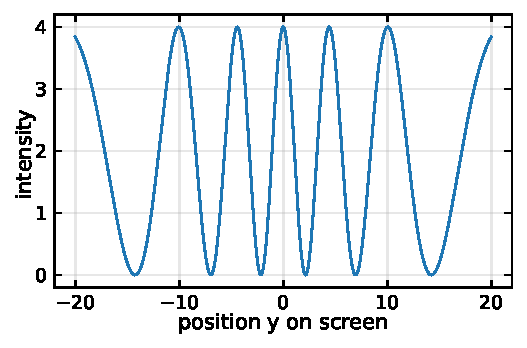
\includegraphics[keepaspectratio]{wave-optics/Double Slit_files/figure-pdf/cell-4-output-1.pdf}}

}

\caption{Intensity pattern of two sources at a screen at a distance L.
The sources are separated by a distance d and the wavelength of the
waves is \(\lambda\).}

\end{figure}%

\section{Application: Optical Resolution and
Imaging}\label{application-optical-resolution-and-imaging}

The physics of two-source interference has profound implications for the
resolution of optical instruments---the fundamental limit on how closely
spaced two objects can be and still be distinguished as separate. This
connection between interference and resolution was recognized by Ernst
Abbe in the 1870s and forms the theoretical foundation for modern
microscopy.

Consider two point sources (such as two stars viewed through a
telescope, or two fluorescent molecules under a microscope). Each source
produces its own diffraction pattern, and these patterns overlap on the
detector. When the sources are far apart, their patterns are well
separated and easily distinguished. But as we bring them closer
together, their patterns overlap more and more. Eventually, they become
so close that we can no longer tell whether we're seeing two sources or
just one extended source.

The \textbf{Rayleigh criterion} provides a practical definition of
resolution: two sources are considered ``just resolved'' when the
central maximum of one diffraction pattern falls on the first minimum of
the other. For a circular aperture (like most telescope and microscope
objectives), this leads to a minimum resolvable angular separation of:

\begin{tcolorbox}[enhanced jigsaw, breakable, toptitle=1mm, bottomrule=.15mm, colbacktitle=quarto-callout-important-color!10!white, title=\textcolor{quarto-callout-important-color}{\faExclamation}\hspace{0.5em}{Optical Resolution Limits}, arc=.35mm, rightrule=.15mm, bottomtitle=1mm, opacityback=0, toprule=.15mm, coltitle=black, leftrule=.75mm, opacitybacktitle=0.6, colback=white, left=2mm, titlerule=0mm, colframe=quarto-callout-important-color-frame]

\textbf{Rayleigh criterion (angular resolution):}

In one of our later lectures we will discuss the derivation of this
formula.

\[\theta_{\text{min}} = 1.22\frac{\lambda}{D}\]

where \(D\) is the diameter of the aperture (lens or mirror).

\textbf{Abbe diffraction limit (spatial resolution):}
\[d_{\text{min}} = \frac{\lambda}{2n\sin(\theta)} = \frac{\lambda}{2\text{NA}}\]

where:

\begin{itemize}
\tightlist
\item
  \(n\) = refractive index of the medium
\item
  \(\theta\) = half-angle of the cone of light collected by the
  objective
\item
  NA = \(n\sin(\theta)\) is the \textbf{numerical aperture} of the
  objective
\end{itemize}

\textbf{Key implications:}

\begin{itemize}
\tightlist
\item
  \textbf{Smaller wavelength improves resolution:} This is why electron
  microscopes (using electron waves with \(\lambda \sim 0.001\) nm) can
  resolve atomic structures, while optical microscopes
  (\(\lambda \sim 500\) nm) cannot.
\item
  \textbf{Larger apertures improve resolution:} Astronomical telescopes
  are built as large as possible partly to achieve better angular
  resolution.
\item
  \textbf{Higher numerical aperture improves resolution:} Modern
  microscopy objectives achieve NA up to \textasciitilde1.4 by using oil
  immersion (\(n \approx 1.5\)) and large collection angles.
\end{itemize}

\textbf{Practical example:} A high-end optical microscope with NA = 1.4
and \(\lambda = 500\) nm can resolve features as small as
\(d_{\text{min}} \approx 180\) nm---about \(\lambda/3\). This is why we
cannot see individual viruses (typically 20-300 nm) with optical
microscopes but can see bacteria (typically \textgreater{} 1 µm).

\end{tcolorbox}

The Abbe limit is not merely a practical limitation---it's a fundamental
consequence of wave physics. Overcoming this limit requires
fundamentally different approaches, such as super-resolution microscopy
techniques (which earned the 2014 Nobel Prize in Chemistry), near-field
scanning methods, or shorter wavelengths like X-rays or electron beams.

\section{Application: Spectroscopy and Wavelength
Analysis}\label{application-spectroscopy-and-wavelength-analysis}

The sensitivity of the double slit interference pattern to wavelength
makes it an excellent tool for spectroscopy---the analysis of light by
its wavelength composition. When white light (containing all visible
wavelengths) passes through a double slit, each wavelength produces its
own set of fringes at slightly different angles according to
\(\sin(\theta) = m\lambda/d\). This separates the light into a spectrum,
with violet (\(\lambda \approx 400\) nm) appearing at smaller angles and
red (\(\lambda \approx 700\) nm) at larger angles.

Practical spectrometers typically use diffraction gratings---devices
with thousands of parallel slits---rather than just two slits. However,
the underlying physics is identical to the double slit, and the same
\(\lambda/d\) relationship governs the angular dispersion. By measuring
the angles at which different wavelengths appear, we can determine the
wavelength composition of light sources. This technique is ubiquitous in
science:

\begin{itemize}
\tightlist
\item
  \textbf{Astronomy:} Identifying elements in distant stars and galaxies
  through their spectral lines
\item
  \textbf{Chemistry:} Determining molecular composition through
  absorption and emission spectroscopy
\item
  \textbf{Environmental monitoring:} Detecting pollutants and measuring
  concentrations
\item
  \textbf{Telecommunications:} Analyzing and multiplexing optical
  signals at different wavelengths
\end{itemize}

The resolving power of a spectrometer---its ability to distinguish
between two closely spaced wavelengths---improves with the total number
of slits illuminated, demonstrating again how multi-wave interference
(discussed in the Multiple Wave Interference lecture) builds on the
two-slit foundation we've developed here.

\section{Historical Context: Fresnel's
Experiments}\label{historical-context-fresnels-experiments}

While Thomas Young's double slit experiment (1801) provided the first
clear evidence for the wave nature of light, Augustin-Jean Fresnel
developed several elegant variations in the 1810s-1820s that removed
potential objections and further solidified the wave theory. These
experiments are worth studying not just for historical reasons, but
because they demonstrate important principles about coherent source
creation and optical path manipulation.

\subsection{Fresnel Double Mirror}\label{fresnel-double-mirror}

In the Fresnel double mirror experiment, a single light source is placed
in front of two plane mirrors tilted at a small angle to each other.
Each mirror creates a virtual image of the source, and these two virtual
images act as coherent sources that produce an interference pattern on a
screen. The key advantage of this configuration is that it unambiguously
creates two coherent sources from a single original source, eliminating
concerns about whether the two slits in Young's experiment might somehow
create incoherent light.

\begin{figure}[H]

{\centering 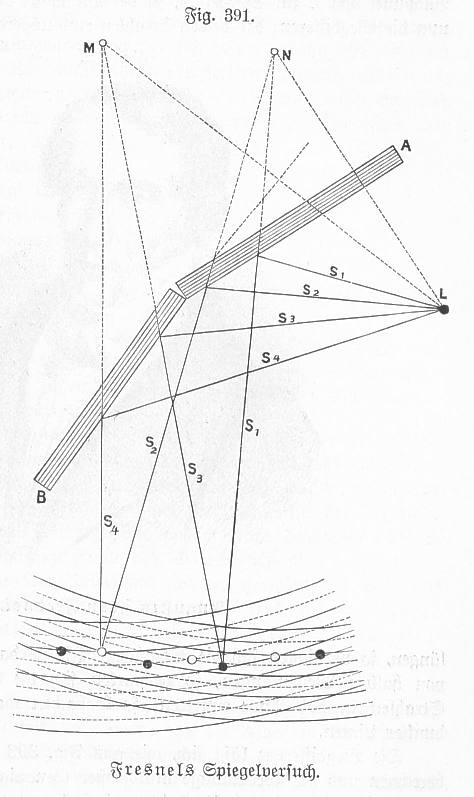
\includegraphics[width=0.6\linewidth,height=\textheight,keepaspectratio]{wave-optics/img/fresnel_alt.jpg}

}

\caption{Fresnel double mirror experiment}

\end{figure}%

The geometry ensures that light paths from the source to each mirror and
then to the screen maintain the coherence necessary for stable
interference. The separation between the virtual sources can be
controlled by adjusting the angle between the mirrors, allowing
systematic study of how fringe spacing depends on source
separation---directly confirming the \(d\) dependence in our
interference formulas.

\subsection{Fresnel Biprism}\label{fresnel-biprism}

The Fresnel biprism offers another ingenious method for creating two
coherent sources. This device consists of two thin prisms joined at
their bases, with very small apex angles. When light from a single
source passes through the biprism, it's refracted in opposite directions
by the two prism halves, creating two virtual sources behind the
biprism. These virtual sources are mutually coherent and produce the
characteristic double-slit interference pattern.

\begin{figure}[H]

{\centering 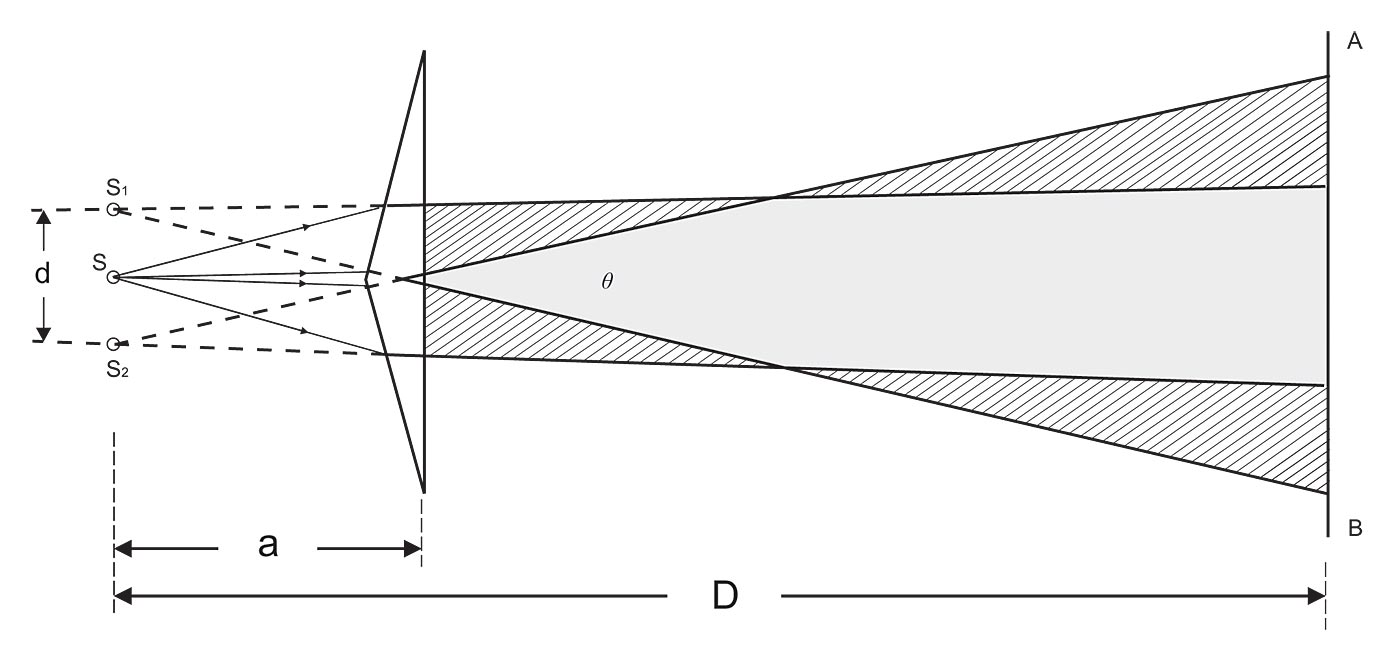
\includegraphics[width=0.6\linewidth,height=\textheight,keepaspectratio]{wave-optics/img/fresnel_biprism.jpg}

}

\caption{Fresnel biprism experiment}

\end{figure}%

The biprism experiment is particularly elegant because it makes the wave
interpretation almost inescapable. The continuous glass surface clearly
transmits the wave from a single source, splitting it into two paths
that later recombine. There's no opportunity for the light to somehow
``choose'' which path to take in discrete packets, as corpuscular
theories might suggest. The wave must propagate through both halves of
the biprism simultaneously, interfering with itself at the recombination
point.

Both of these experiments, along with Young's original double slit,
played crucial roles in establishing the wave theory of light in the
19th century. They demonstrate the fundamental principle that coherent
sources for interference can be created by splitting light from a single
source and allowing the split beams to travel different paths before
recombining---a principle that underlies all modern interferometry.

\section{Conclusion}\label{conclusion-1}

The double slit experiment and its variations reveal the wave nature of
light through the unmistakable signature of interference. The simple
relationship \(\Delta s = d\sin(\theta)\) between path difference and
observation angle, combined with the phase condition for constructive
interference, allows us to predict exactly where bright and dark fringes
will appear. This same physics governs phenomena ranging from the
resolution limits of microscopes to the operation of spectrometers that
analyze starlight from distant galaxies.

Beyond its practical applications, the double slit experiment continues
to challenge and deepen our understanding of quantum mechanics. When
performed with single photons or electrons, the interference pattern
builds up particle by particle, suggesting that each particle somehow
``interferes with itself'' by exploring both paths simultaneously. This
quantum version of the double slit experiment reveals the wave-particle
duality at the heart of quantum theory and reminds us that even the
simplest optical experiment can open doors to profound questions about
the nature of reality.

The principles we've developed here---calculating path differences,
relating phase to interference, and understanding the \(\lambda/d\)
scaling of interference patterns---form the foundation for the more
complex interferometric devices and multiple-wave interference phenomena
we'll explore in subsequent lectures. The double slit may be simple in
concept, but its implications echo throughout all of wave optics and
quantum physics.

\chapter{Interferometers and other Coherence
Applications}\label{interferometers-and-other-coherence-applications}

Interferometry is fundamentally based on the principle that light waves
accumulate phase as they propagate through space. The key to
understanding how interferometers work lies in recognizing the
relationship between the optical path length traveled by light and the
phase it accumulates along that path. When a light wave travels through
a medium with refractive index \(n\) over a physical distance \(L\), it
accumulates an optical path length (OPL) given by
\(\text{OPL} = n \cdot L\). The phase acquired by the light wave is then
directly proportional to this optical path length, expressed as
\(\phi = \frac{2\pi}{\lambda} \text{OPL}\), where \(\lambda\) is the
wavelength of light in vacuum.

This relationship has profound implications for interferometric
measurements. When we split a beam of light into two paths and then
recombine them, the resulting interference pattern depends on the phase
difference between the two beams.

\begin{tcolorbox}[enhanced jigsaw, breakable, toptitle=1mm, bottomrule=.15mm, colbacktitle=quarto-callout-important-color!10!white, title=\textcolor{quarto-callout-important-color}{\faExclamation}\hspace{0.5em}{Fundamental Phase Difference Formula}, arc=.35mm, rightrule=.15mm, bottomtitle=1mm, opacityback=0, toprule=.15mm, coltitle=black, leftrule=.75mm, opacitybacktitle=0.6, colback=white, left=2mm, titlerule=0mm, colframe=quarto-callout-important-color-frame]

\[\Delta \phi = \frac{2\pi}{\lambda}(n_1 L_1 - n_2 L_2)\]

This is the cornerstone equation of interferometry. The phase difference
\(\Delta \phi\) between two light beams depends on the difference in
their optical path lengths. Here, \(\lambda\) is the wavelength of
light, \(n_1\) and \(n_2\) are the refractive indices along each path,
and \(L_1\) and \(L_2\) are the physical path lengths. This formula
reveals two fundamental ways to create a phase difference:

\begin{enumerate}
\def\labelenumi{\arabic{enumi}.}
\tightlist
\item
  \textbf{Change the physical path length} (\(L\)) - used in LIGO,
  precision metrology
\item
  \textbf{Change the refractive index} (\(n\)) - used in gas sensing,
  electro-optic modulators
\end{enumerate}

\end{tcolorbox}

From this expression, we can immediately see that there are two distinct
ways to introduce a phase difference: we can either change the physical
length of one path (varying \(L\)), or we can change the refractive
index along one path (varying \(n\)). This duality is what makes
interferometers incredibly versatile instruments, capable of measuring
not only distances and mechanical vibrations but also changes in the
optical properties of materials, gas composition, temperature, and even
rotation.

The interference that results from this phase difference manifests as
alternating bright and dark fringes.

\begin{tcolorbox}[enhanced jigsaw, breakable, toptitle=1mm, bottomrule=.15mm, colbacktitle=quarto-callout-tip-color!10!white, title=\textcolor{quarto-callout-tip-color}{\faLightbulb}\hspace{0.5em}{Interference Conditions}, arc=.35mm, rightrule=.15mm, bottomtitle=1mm, opacityback=0, toprule=.15mm, coltitle=black, leftrule=.75mm, opacitybacktitle=0.6, colback=white, left=2mm, titlerule=0mm, colframe=quarto-callout-tip-color-frame]

\textbf{Constructive interference (bright fringes):}
\(\Delta \phi = 2\pi m\) where \(m = 0, 1, 2, 3, ...\)

\textbf{Destructive interference (dark fringes):}
\(\Delta \phi = \pi(2m + 1)\) where \(m = 0, 1, 2, 3, ...\)

These conditions determine when light waves add constructively (maximum
intensity) or destructively (minimum intensity).

\end{tcolorbox}

By carefully observing how these interference patterns change, we can
extract extremely precise measurements of whatever physical quantity is
causing the phase shift.

A critical requirement for all interferometric measurements is
\textbf{coherence}---the light beams must maintain a stable phase
relationship over the time and distance scales of the measurement. As
discussed in the lecture on interference, coherence is characterized by
the coherence length \(L_c = c\tau_c\), where \(\tau_c = 1/\Delta\nu\)
is the coherence time and \(\Delta\nu\) is the spectral bandwidth of the
light source. For an interferometer to produce stable interference
fringes, the optical path difference between the interfering beams must
be smaller than the coherence length. This is why modern interferometers
almost universally employ lasers as light sources: a typical HeNe laser
has a coherence length of tens of centimeters to meters, while a
stabilized single-mode laser can have coherence lengths of kilometers.
In contrast, white light from a thermal source has a coherence length of
only a few micrometers, making it unsuitable for most interferometric
applications (though it can be used for specialized techniques like
white light interferometry for surface profiling).

In the following sections, we will explore several important types of
interferometers and examine how they exploit these principles for
various scientific and technological applications.

\section{Michelson Interferometer}\label{michelson-interferometer}

The Michelson interferometer is perhaps the most fundamental and
historically significant optical interferometer. Its basic design
elegantly demonstrates the core principles of interferometry while
providing a platform for extraordinarily precise measurements. The
interferometer consists of a coherent light source, typically a laser,
that emits a beam directed toward a beam splitter positioned at 45
degrees to the incoming beam. This beam splitter divides the incident
light into two beams of approximately equal intensity: one beam is
reflected at 90 degrees toward a fixed mirror, while the other is
transmitted straight through toward a movable mirror. After reflecting
off their respective mirrors, both beams return to the beam splitter
where they are recombined, with portions of each beam directed toward a
detector or viewing screen where they interfere.

\begin{figure}[H]

{\centering 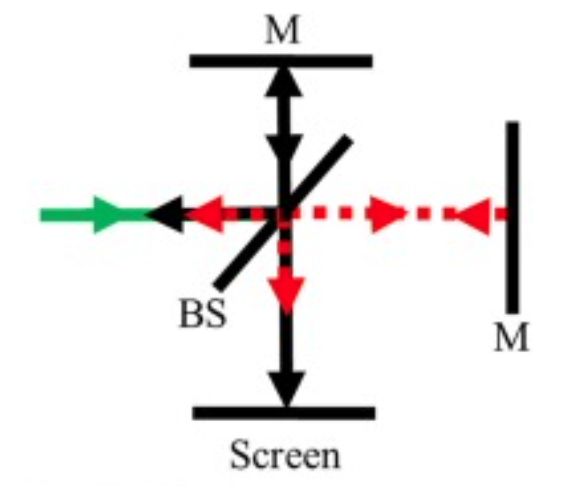
\includegraphics[width=0.3\linewidth,height=\textheight,keepaspectratio]{wave-optics/img/michelson.png}

}

\caption{Michelson Interferometer}

\end{figure}%

The key to understanding the Michelson interferometer lies in analyzing
the optical path difference between the two arms. If we denote the
distance from the beam splitter to the fixed mirror as \(L_1\) and the
distance to the movable mirror as \(L_2\), then the total optical path
difference is \(\Delta L = 2(L_2 - L_1)\), where the factor of 2
accounts for the round trip each beam makes to its respective mirror and
back. This path difference translates directly into a phase difference
of \(\Delta \phi = \frac{4\pi(L_2 - L_1)}{\lambda}\). When
\(L_1 = L_2\), the beams interfere constructively. As we move the
movable mirror by a distance \(d\), we introduce a path difference of
\(2d\), and each time this path difference changes by one wavelength, we
observe one complete cycle of the interference pattern---from bright to
dark and back to bright again.

\subsection{Application: Measuring Refractive Index of
Gases}\label{application-measuring-refractive-index-of-gases}

One of the most elegant applications of the Michelson interferometer is
the measurement of the refractive index of gases. This technique
demonstrates beautifully how interferometers can detect not just changes
in geometric path length, but also changes in optical path length due to
variations in the refractive index. To perform this measurement, we
place a transparent gas cell of known length \(L\) in one arm of the
interferometer. Initially, when the cell is evacuated and contains only
vacuum, the optical path through that arm is simply
\(n_{\text{vacuum}} \cdot L = L\) (since \(n_{\text{vacuum}} = 1\)).
When we introduce a gas into the cell, the refractive index changes from
1 to \(n_{\text{gas}}\), which slightly increases the optical path
length in that arm to \(n_{\text{gas}} \cdot L\).

The change in optical path length is
\(\Delta(\text{OPL}) = (n_{\text{gas}} - 1)L\). Since the light makes a
round trip through the cell, the total change in optical path length is
\(2(n_{\text{gas}} - 1)L\). This change manifests as a shift in the
interference pattern.

\begin{tcolorbox}[enhanced jigsaw, breakable, toptitle=1mm, bottomrule=.15mm, colbacktitle=quarto-callout-important-color!10!white, title=\textcolor{quarto-callout-important-color}{\faExclamation}\hspace{0.5em}{Gas Refractive Index Measurement Formula}, arc=.35mm, rightrule=.15mm, bottomtitle=1mm, opacityback=0, toprule=.15mm, coltitle=black, leftrule=.75mm, opacitybacktitle=0.6, colback=white, left=2mm, titlerule=0mm, colframe=quarto-callout-important-color-frame]

\[n_{\text{gas}} = 1 + \frac{m\lambda}{2L}\]

This formula allows us to determine the refractive index of a gas by
counting fringe shifts. Here:

\begin{itemize}
\tightlist
\item
  \(m\) = number of bright fringes that pass by as the cell is filled
\item
  \(\lambda\) = wavelength of light used
\item
  \(L\) = length of the gas cell
\end{itemize}

\textbf{How it works:} Place a gas cell of length \(L\) in one arm of
the interferometer. As you fill it with gas, the refractive index
changes from 1 (vacuum) to \(n_{\text{gas}}\), causing fringes to shift.
Count the fringes to determine \(n_{\text{gas}}\).

\end{tcolorbox}

Specifically, if we count the number of bright fringes \(m\) that pass
by a reference point as we fill the cell with gas, we can relate this to
the refractive index through the equation
\(m = \frac{2(n_{\text{gas}} - 1)L}{\lambda}\), which can be rearranged
to give the formula above.

For example, if we use a HeNe laser with \(\lambda = 632.8\) nm and a
gas cell of length \(L = 10\) cm, and we observe 20 fringes passing as
we fill the cell with air at standard conditions, we can calculate that
the refractive index of air is approximately
\(n_{\text{air}} \approx 1.000063\). This technique is remarkably
sensitive; even tiny changes in gas pressure, temperature, or
composition can be detected by monitoring the interference pattern. This
makes the Michelson interferometer valuable for applications ranging
from gas sensing and environmental monitoring to quality control in
industrial processes.

\subsection{Application: The LIGO Gravitational Wave
Detector}\label{application-the-ligo-gravitational-wave-detector}

The extraordinary sensitivity of the Michelson interferometer to changes
in path length reaches its ultimate expression in the Laser
Interferometer Gravitational-Wave Observatory, or LIGO. This instrument
represents one of the most ambitious and technically challenging
scientific instruments ever constructed, designed to detect
gravitational waves---ripples in the fabric of spacetime itself
predicted by Einstein's general theory of relativity. These waves are
generated by some of the most violent events in the universe, such as
the collision and merger of black holes or neutron stars, and they
propagate through space at the speed of light, stretching and
compressing spacetime as they pass.

\begin{figure}[H]

{\centering \pandocbounded{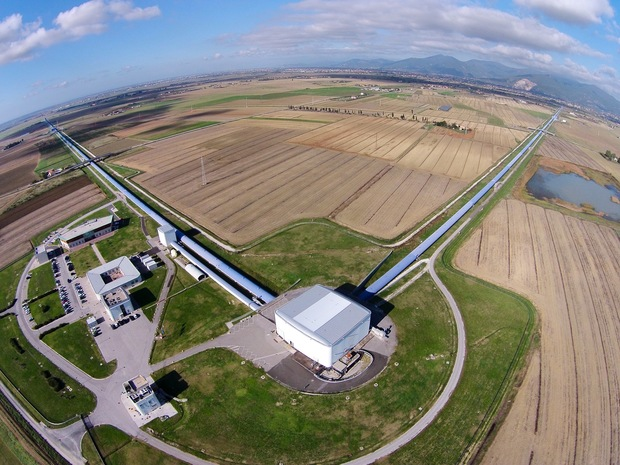
\includegraphics[keepaspectratio]{wave-optics/img/VIRGO.jpg}}

}

\caption{Virgo detector of LIGO}

\end{figure}%

LIGO consists of two large Michelson interferometers located at separate
sites in the United States: one in Hanford, Washington, and the other in
Livingston, Louisiana. Each interferometer has two perpendicular arms
extending 4 kilometers in length. A powerful laser beam is split and
sent down these arms, where it bounces back and forth many times in
Fabry-Pérot cavities before returning to the beam splitter. Under normal
conditions, the interferometer is carefully tuned so that the two beams
interfere destructively when they recombine, meaning essentially no
light reaches the photodetector---this is called the ``dark fringe''
operating point.

When a gravitational wave passes through the detector, it causes one arm
to stretch while simultaneously causing the other arm to compress. This
differential change in length, though incredibly tiny, alters the
optical path difference between the two arms and thus shifts the
interference pattern away from the dark fringe. The detector then
registers light, and the amount of light and how it varies with time
encodes information about the gravitational wave. The sensitivity
required is almost incomprehensible: LIGO must detect changes in arm
length smaller than \(10^{-19}\) meters, which is less than
one-thousandth the diameter of a proton. To put this in perspective,
this is equivalent to measuring the distance to the nearest star (4
light-years away) to an accuracy smaller than the width of a human hair.

\begin{tcolorbox}[enhanced jigsaw, breakable, toptitle=1mm, bottomrule=.15mm, colbacktitle=quarto-callout-important-color!10!white, title=\textcolor{quarto-callout-important-color}{\faExclamation}\hspace{0.5em}{LIGO Phase Shift Formula}, arc=.35mm, rightrule=.15mm, bottomtitle=1mm, opacityback=0, toprule=.15mm, coltitle=black, leftrule=.75mm, opacitybacktitle=0.6, colback=white, left=2mm, titlerule=0mm, colframe=quarto-callout-important-color-frame]

\[\Delta \phi = \frac{4\pi \Delta L}{\lambda}\]

This formula describes the phase shift caused by a gravitational wave in
LIGO. Here: - \(\Delta L\) = change in arm length due to the
gravitational wave - \(\lambda\) = wavelength of the laser (1064 nm for
LIGO) - The factor of 4 comes from: 2 (round trip in each arm) × 2
(differential effect between arms)

\textbf{Why factor of 4?} When a gravitational wave passes through: one
arm increases by \(\Delta L\) while the other decreases by \(\Delta L\).
The light makes a round trip in each arm, so the total optical path
difference is \(2 \cdot 2\Delta L = 4\Delta L\).

\end{tcolorbox}

The phase shift \(\Delta \phi\) caused by a gravitational wave can be
expressed as shown above. To understand this more carefully, consider
that when a gravitational wave passes through the interferometer, it
causes a time-varying strain in spacetime. If one arm increases in
length by \(\Delta L\), the other decreases by approximately the same
amount. The round-trip optical path difference between the arms becomes
\(2 \cdot 2\Delta L = 4\Delta L\), leading to the phase shift formula
given above.

The extraordinary precision of LIGO's measurements is achieved through a
combination of advanced technologies including powerful stabilized
lasers, ultra-high vacuum systems, sophisticated vibration isolation,
and quantum noise reduction techniques. Since its first detection of
gravitational waves in September 2015, LIGO has opened an entirely new
window onto the universe, allowing us to observe cosmic events that are
completely invisible to conventional telescopes. This remarkable
achievement demonstrates how the simple principles of the Michelson
interferometer, when pushed to their ultimate limits, can reveal
phenomena at the very frontiers of physics.

\begin{tcolorbox}[enhanced jigsaw, breakable, toptitle=1mm, bottomrule=.15mm, colbacktitle=quarto-callout-note-color!10!white, title=\textcolor{quarto-callout-note-color}{\faInfo}\hspace{0.5em}{LIGO Technical Details}, arc=.35mm, rightrule=.15mm, bottomtitle=1mm, opacityback=0, toprule=.15mm, coltitle=black, leftrule=.75mm, opacitybacktitle=0.6, colback=white, left=2mm, titlerule=0mm, colframe=quarto-callout-note-color-frame]

LIGO consists of two large interferometers located in the United States:
one in Hanford, Washington, and the other in Livingston, Louisiana.
These facilities are operated by the LIGO Scientific Collaboration
(LSC), which includes scientists from various institutions around the
world. Here is a link to the \href{https://www.ligo.caltech.edu/}{LIGO
website} and a direct link to an
\href{https://www.ligo.caltech.edu/system/media_files/binaries/303/original/ligo-educators-guide.pdf?1455165573}{overview
document}.

The interferometer design employs a Michelson interferometer
configuration with 4-kilometer-long arms forming an ``L'' shape. Each
arm contains a Fabry-Pérot cavity to increase the effective path length
of the laser beams. These cavities are formed by highly reflective
mirrors placed at the ends of the arms, and the laser beams bounce back
and forth multiple times within the cavities, effectively increasing the
arm length to several hundred kilometers. The laser system uses a
high-power, stabilized laser operating at a wavelength of 1064 nm in the
infrared. The laser power is typically around 200 watts, but the
effective power in the interferometer arms is increased to several
kilowatts using power recycling techniques.

The mirrors and other optical components are suspended by a system of
pendulums to isolate them from ground vibrations and other noise
sources. The suspension system includes multiple stages of isolation,
including active and passive damping mechanisms. The interferometer arms
are housed in ultra-high vacuum tubes to eliminate air molecules that
could scatter the laser beams and introduce noise, maintaining a
pressure of around \(10^{-9}\) torr.

Gravitational waves are detected through their effect on the
interference pattern. As a gravitational wave passes through the
interferometer, it stretches and compresses the spacetime along the
arms, causing tiny changes in the arm lengths. These changes cause a
phase shift in the laser beams when they recombine at the beam splitter,
resulting in a change in the interference pattern that is detected by
photodetectors. LIGO is designed to detect changes in arm lengths as
small as \(10^{-19}\) meters through advanced noise reduction
techniques.

The data from the photodetectors are processed using advanced algorithms
and computational techniques to filter out noise and extract potential
gravitational wave signals. When a potential event is detected, the data
are analyzed to determine the properties of the source, such as the
masses and spins of merging black holes or neutron stars. Detection is
confirmed by comparing data from both LIGO detectors and, if available,
data from other gravitational wave observatories like Virgo in Europe.

\end{tcolorbox}

\section{Mach-Zehnder Interferometer}\label{mach-zehnder-interferometer}

The Mach-Zehnder interferometer represents a different geometric
configuration that offers distinct advantages for certain applications,
particularly those involving the manipulation and modulation of light in
optical systems. Unlike the Michelson interferometer where the two beams
travel back and forth along the same paths, the Mach-Zehnder
interferometer splits a beam into two separate paths that never retrace
themselves, and the beams are recombined at a different location from
where they were split. This architecture makes it particularly suitable
for applications where you want to place samples or active devices in
one or both paths without the complications of retroreflection.

\begin{figure}[H]

{\centering 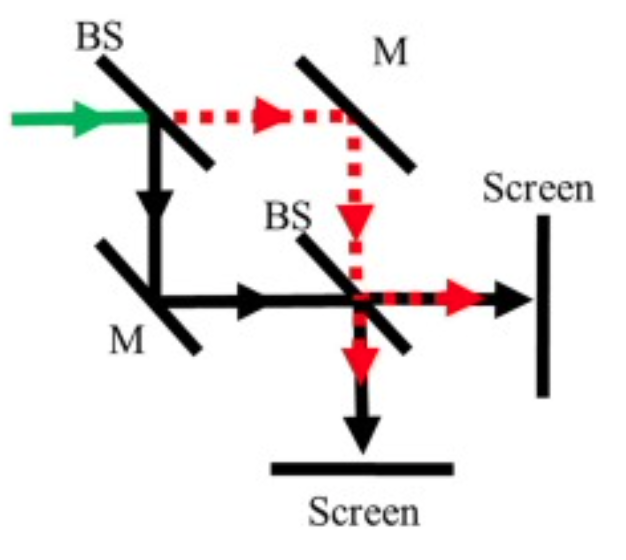
\includegraphics[width=0.3\linewidth,height=\textheight,keepaspectratio]{wave-optics/img/mach.png}

}

\caption{Mach Zehnder Interferometer}

\end{figure}%

The interferometer consists of a coherent light source that emits a beam
toward a first beam splitter, which divides the light into two beams of
approximately equal intensity. These two beams propagate along separate
paths, each encountering a mirror that redirects them toward a second
beam splitter. At this second beam splitter, the two beams are
recombined and directed toward two output ports. The relative phase
between the two beams when they arrive at the second beam splitter
determines the interference pattern and consequently how much light
exits from each output port. If the two paths have exactly the same
optical path length, the beams arrive in phase at the second beam
splitter, and the interference is purely constructive at one output port
and destructive at the other.

\begin{tcolorbox}[enhanced jigsaw, breakable, toptitle=1mm, bottomrule=.15mm, colbacktitle=quarto-callout-tip-color!10!white, title=\textcolor{quarto-callout-tip-color}{\faLightbulb}\hspace{0.5em}{Mach-Zehnder Phase Difference}, arc=.35mm, rightrule=.15mm, bottomtitle=1mm, opacityback=0, toprule=.15mm, coltitle=black, leftrule=.75mm, opacitybacktitle=0.6, colback=white, left=2mm, titlerule=0mm, colframe=quarto-callout-tip-color-frame]

\[\Delta \phi = \frac{2\pi}{\lambda}(n_1 L_1 - n_2 L_2)\]

Unlike the Michelson interferometer, the Mach-Zehnder uses
non-retroreflecting paths (no factor of 2 from round trips). The phase
difference depends on:

\begin{itemize}
\tightlist
\item
  \(L_1, L_2\) = physical path lengths of the two arms
\item
  \(n_1, n_2\) = refractive indices along each arm
\end{itemize}

By controlling either the path length or refractive index in one arm, we
can switch light between output ports.

\end{tcolorbox}

By introducing changes to either the path length or the refractive index
in one arm, we can control the phase difference and thereby switch the
light between the two output ports. This controllability makes the
Mach-Zehnder interferometer ideal for applications in optical
communications, sensing, and information processing.

\begin{figure}

\begin{minipage}{0.50\linewidth}

\begin{figure}[H]

{\centering \pandocbounded{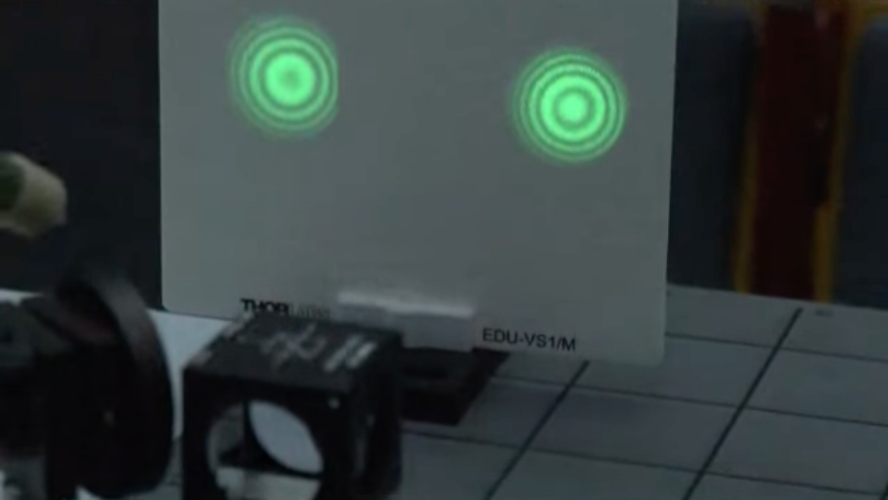
\includegraphics[keepaspectratio]{wave-optics/img/machz_lecture_pat.png}}

}

\subcaption{Mach Zehnder Interferometer with a Gaussian}

\end{figure}%

\end{minipage}%
%
\begin{minipage}{0.50\linewidth}

\begin{figure}[H]

{\centering \pandocbounded{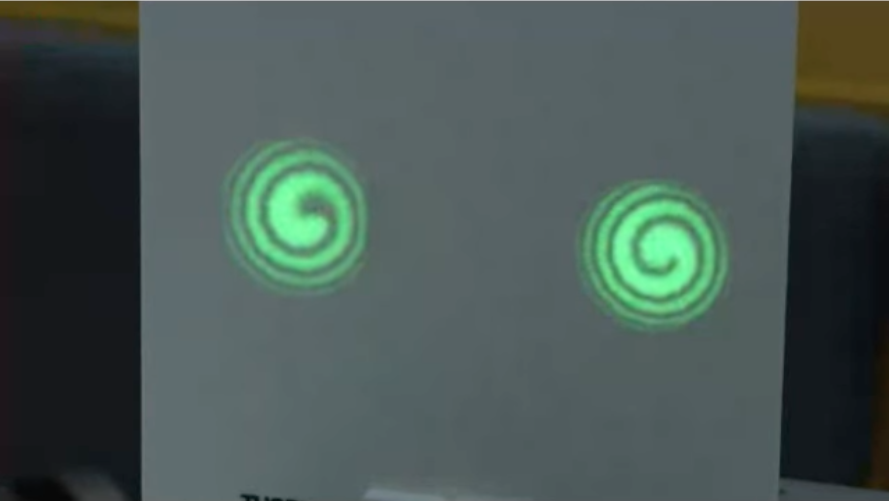
\includegraphics[keepaspectratio]{wave-optics/img/machz_lecture_vortex.png}}

}

\subcaption{Mach Zehnder Interferometer with a Bessel Beam}

\end{figure}%

\end{minipage}%

\end{figure}%

\subsection{Application: Electro-Optic Modulators in Photonic Integrated
Circuits}\label{application-electro-optic-modulators-in-photonic-integrated-circuits}

One of the most important modern applications of the Mach-Zehnder
interferometer is in electro-optic phase modulators, particularly those
implemented on photonic integrated circuits. These devices are essential
components in fiber-optic communication systems, optical computing, and
various sensing applications. The basic principle involves placing an
electro-optic material---a material whose refractive index changes in
response to an applied electric field---in one or both arms of the
interferometer. When voltage is applied to electrodes positioned near
the waveguides, the resulting electric field modulates the refractive
index of the material through the Pockels effect, thereby changing the
optical path length in that arm and introducing a phase shift.

In a typical integrated Mach-Zehnder modulator fabricated on a
\emph{lithium niobate} substrate or \emph{silicon photonic} platform,
light enters the device and is split equally into two waveguide arms.
Electrodes are patterned along one or both arms, and when a voltage
\(V\) is applied, it creates an electric field that changes the
refractive index by an amount proportional to the applied field.

\begin{tcolorbox}[enhanced jigsaw, breakable, toptitle=1mm, bottomrule=.15mm, colbacktitle=quarto-callout-important-color!10!white, title=\textcolor{quarto-callout-important-color}{\faExclamation}\hspace{0.5em}{Electro-Optic Phase Modulation (Pockels Effect)}, arc=.35mm, rightrule=.15mm, bottomtitle=1mm, opacityback=0, toprule=.15mm, coltitle=black, leftrule=.75mm, opacitybacktitle=0.6, colback=white, left=2mm, titlerule=0mm, colframe=quarto-callout-important-color-frame]

\textbf{Refractive index change:} \[\Delta n = -\frac{1}{2}n^3 r E\]

\textbf{Resulting phase shift:}
\[\Delta \phi = \frac{2\pi}{\lambda} \Delta n \cdot L\]

where:

\begin{itemize}
\tightlist
\item
  \(n\) = unperturbed refractive index
\item
  \(r\) = Pockels coefficient (material property)
\item
  \(E\) = applied electric field
\item
  \(L\) = length of the modulator arm
\item
  \(\lambda\) = wavelength of light
\end{itemize}

\textbf{Key principle:} Applying voltage changes the electric field
\(E\), which changes the refractive index \(\Delta n\) via the Pockels
effect, which in turn changes the phase \(\Delta \phi\). This
voltage-controlled phase shift enables high-speed optical modulation for
telecommunications and photonic computing.

\end{tcolorbox}

When the beams recombine at the output, the interference pattern depends
on this voltage-controlled phase shift. By varying the applied voltage,
we can continuously tune the output intensity from maximum (constructive
interference) to minimum (destructive interference) and back again. This
allows us to encode electrical signals onto optical carriers, converting
the electrical voltage signal into variations in optical intensity---a
process essential for transmitting data through optical fibers. The
speed at which these modulators can operate is determined by the
response time of the electro-optic effect and the electrical bandwidth
of the device, with state-of-the-art modulators achieving modulation
rates exceeding 100 GHz.

Beyond telecommunications, Mach-Zehnder modulators are now finding
applications in emerging photonic computing systems. Arrays of
interconnected Mach-Zehnder interferometers can be configured to perform
matrix multiplication operations optically, which is a fundamental
operation in neural networks and machine learning algorithms. In these
systems, the phase shifters in each Mach-Zehnder element are programmed
to represent the weights of the neural network, and the optical signals
propagating through the network perform the computations at the speed of
light with potentially much lower energy consumption than electronic
processors.

\begin{figure}[H]

{\centering \pandocbounded{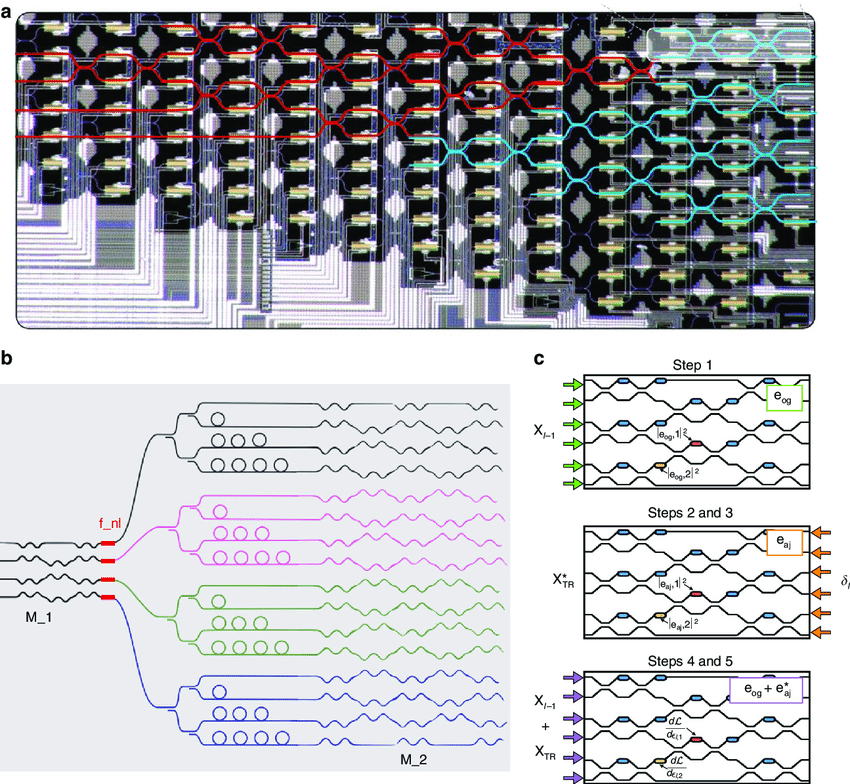
\includegraphics[keepaspectratio]{wave-optics/img/MZI-ONN.png}}

}

\caption{Network of Mach Zehnder Interferometers forming an all optical
neural network. Zhou, H. et al.~Photonic matrix multiplication lights up
photonic accelerator and beyond. Light: Sci. Appl. 11, 30 (2022).}

\end{figure}%

This image illustrates a sophisticated implementation where multiple
Mach-Zehnder interferometers are arranged in a network to create an
all-optical neural network processor. Each interferometer acts as a
programmable element that can be tuned to implement specific
mathematical operations, and the entire network performs complex
computations by manipulating the phase and amplitude of light waves as
they propagate through the structure. This represents a powerful
demonstration of how the simple principle of interference can be scaled
up and integrated to create advanced photonic systems with applications
in artificial intelligence and high-speed information processing.

\section{Sagnac Interferometer}\label{sagnac-interferometer}

The Sagnac interferometer operates on a fundamentally different
principle from the Michelson and Mach-Zehnder interferometers we have
discussed so far. While those devices are sensitive to differences in
path length or refractive index between two spatially separated paths,
the Sagnac interferometer is specifically designed to detect rotation.
This unique capability has made it the basis for highly accurate
fiber-optic gyroscopes used in aircraft navigation, spacecraft attitude
control, and autonomous vehicle systems.

\begin{figure}[H]

{\centering 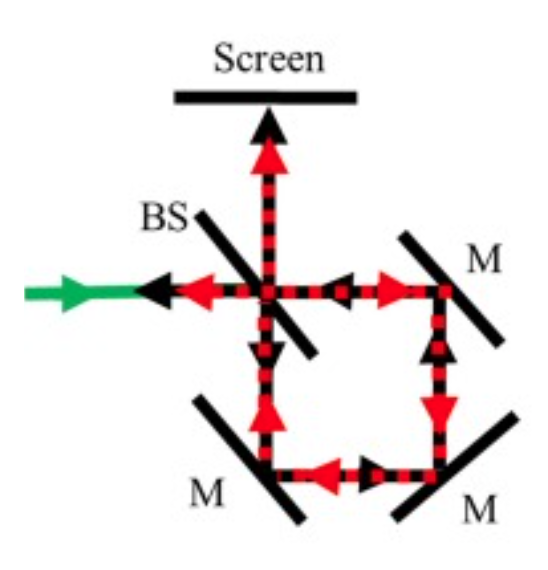
\includegraphics[width=0.3\linewidth,height=\textheight,keepaspectratio]{wave-optics/img/sagnac.png}

}

\caption{Sagnac Interferometer}

\end{figure}%

In a Sagnac interferometer, a beam of light is split into two beams that
travel around the same closed loop but in opposite directions---one
clockwise and the other counterclockwise. These counter-propagating
beams are then recombined after completing their journeys around the
loop. In a non-rotating reference frame, both beams travel exactly the
same path and accumulate the same phase, resulting in perfect
constructive interference when they recombine. However, when the entire
interferometer is rotating, something remarkable happens: the two beams
experience different effective path lengths despite traveling along the
same physical path. This is a consequence of the fact that, in the
rotating frame of the interferometer, the point where the beams
recombine is moving. From the perspective of the laboratory frame, the
beam traveling in the direction of rotation has a slightly longer path
to travel to reach the recombination point, while the beam traveling
opposite to the rotation has a slightly shorter path.

\subsection{Derivation and Application in Fiber-Optic
Gyroscopes}\label{derivation-and-application-in-fiber-optic-gyroscopes}

The phase shift induced by rotation can be derived by considering the
time difference between the two counter-propagating beams. For an
interferometer loop enclosing an area \(A\) and rotating with angular
velocity \(\Omega\), the time difference \(\Delta T\) between the two
beams can be shown to be \(\Delta T = \frac{4A\Omega}{c^2}\), where
\(c\) is the speed of light. This time difference directly translates
into a phase shift.

\begin{tcolorbox}[enhanced jigsaw, breakable, toptitle=1mm, bottomrule=.15mm, colbacktitle=quarto-callout-important-color!10!white, title=\textcolor{quarto-callout-important-color}{\faExclamation}\hspace{0.5em}{Sagnac Effect: Rotation-Induced Phase Shift}, arc=.35mm, rightrule=.15mm, bottomtitle=1mm, opacityback=0, toprule=.15mm, coltitle=black, leftrule=.75mm, opacitybacktitle=0.6, colback=white, left=2mm, titlerule=0mm, colframe=quarto-callout-important-color-frame]

\[\Delta \phi = \frac{8\pi A \Omega}{\lambda c}\]

This fundamental formula for rotation sensing shows that the phase shift
depends on: - \(A\) = area enclosed by the light path - \(\Omega\) =
angular velocity of rotation - \(\lambda\) = wavelength of light - \(c\)
= speed of light

\textbf{Key insight:} The phase shift is independent of the loop
shape---only the enclosed area matters! A circular, square, or irregular
loop with the same area will have the same sensitivity to rotation.

\textbf{Practical implementation:} In fiber-optic gyroscopes, the fiber
is coiled \(N\) times, giving total area \(A = N \cdot A_0\), which
multiplies the sensitivity by \(N\).

\end{tcolorbox}

This remarkably simple formula shows that the phase shift is directly
proportional to the angular velocity \(\Omega\) and to the area \(A\)
enclosed by the light path, but is independent of the shape of that
path. This is a profound result: whether the loop is circular, square,
or any other shape, only the enclosed area matters for determining the
sensitivity to rotation.

\begin{figure}[H]

{\centering 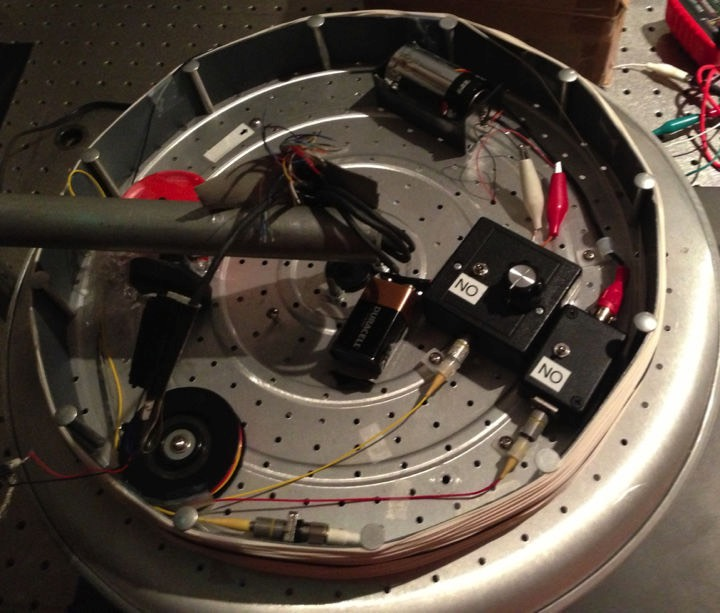
\includegraphics[width=0.5\linewidth,height=\textheight,keepaspectratio]{wave-optics/img/sagnac_exp.png}

}

\caption{Sagnac interferometer made of a fibre rolled up on a cylinder
taken from
\href{https://www.stabilock.com/holography--consulting/fiber-optic-sensors/sagnac-interferometer.html}{here}}

\end{figure}%

In practical fiber-optic gyroscopes, the light path is formed by winding
many turns of optical fiber into a coil. If the fiber is wound into
\(N\) turns, each enclosing an area \(A_0\), then the total effective
area is \(A = N \cdot A_0\), which greatly enhances the sensitivity of
the device. Modern fiber-optic gyroscopes can use coils with hundreds or
even thousands of turns, achieving extraordinary sensitivity to rotation
rates. These devices have several advantages over mechanical gyroscopes:
they have no moving parts, are immune to mechanical wear, can operate
over a wide range of temperatures, and are relatively compact and
lightweight.

The sensitivity of a Sagnac gyroscope can be expressed as the minimum
detectable rotation rate, which depends on the ability to measure small
phase shifts. With modern photodetectors and signal processing
techniques, phase shifts as small as microradians can be detected,
corresponding to rotation rates of fractions of a degree per hour. This
level of performance makes fiber-optic gyroscopes suitable for inertial
navigation systems in commercial aircraft, military vehicles, and
spacecraft, where they provide continuous information about the
vehicle's orientation and angular velocity without requiring any
external reference.

\begin{tcolorbox}[enhanced jigsaw, breakable, toptitle=1mm, bottomrule=.15mm, colbacktitle=quarto-callout-note-color!10!white, title=\textcolor{quarto-callout-note-color}{\faInfo}\hspace{0.5em}{Derivation Details}, arc=.35mm, rightrule=.15mm, bottomtitle=1mm, opacityback=0, toprule=.15mm, coltitle=black, leftrule=.75mm, opacitybacktitle=0.6, colback=white, left=2mm, titlerule=0mm, colframe=quarto-callout-note-color-frame]

To derive the formula for the time difference \(\Delta T\) between two
counter-propagating beams in a Sagnac interferometer, we start by
considering a loop of perimeter \(L\) and area \(A\). The interferometer
is rotating with an angular velocity \(\Omega\). Light travels in
opposite directions around the loop, creating two counter-propagating
beams.

In a non-rotating frame, the time taken for light to travel around the
loop is \(T = \frac{L}{c}\). When the interferometer rotates with
angular velocity \(\Omega\), the effective path lengths for the two
beams differ due to the rotation. For the beam traveling in the
direction of rotation, the effective path length increases, while for
the beam traveling opposite to the direction of rotation, the effective
path length decreases.

The relative velocity of light with respect to the rotating frame is
\(c \pm v\), where \(v = \Omega R\) is the tangential velocity at the
perimeter of the loop. For small angular velocities, we can approximate
the effect using the area \(A\) and the angular velocity \(\Omega\).

The time taken for the beam traveling in the direction of rotation is
\(T_+ = \frac{L}{c - v}\), and the time taken for the beam traveling
opposite to the direction of rotation is \(T_- = \frac{L}{c + v}\). For
small \(v\), we can use the binomial expansion to approximate the times:

\[
T_+ \approx \frac{L}{c}\left(1 + \frac{v}{c}\right), \quad T_- \approx \frac{L}{c}\left(1 - \frac{v}{c}\right)
\]

The time difference between the two beams is:

\[
\Delta T = T_+ - T_- = \frac{L}{c}\left(1 + \frac{v}{c}\right) - \frac{L}{c}\left(1 - \frac{v}{c}\right) = \frac{2Lv}{c^2}
\]

The tangential velocity \(v\) is related to the angular velocity
\(\Omega\) and the effective radius \(R\) of the loop. For a general
loop shape, we can relate the area and perimeter through the geometry of
the loop. For a circular loop, \(A = \pi R^2\) and \(L = 2\pi R\),
giving \(R = \frac{L}{2\pi}\) and thus \(v = \Omega \frac{L}{2\pi}\).

Substituting this into the expression for \(\Delta T\):

\[
\Delta T = \frac{2L \cdot \Omega \frac{L}{2\pi}}{c^2} = \frac{L^2 \Omega}{\pi c^2}
\]

For a circular loop, \(L^2 = 4\pi A\), which gives:

\[
\Delta T = \frac{4\pi A \Omega}{\pi c^2} = \frac{4A\Omega}{c^2}
\]

This result, remarkably, holds for arbitrary loop shapes, not just
circular ones, which can be proven using more general arguments from
relativity theory.

\end{tcolorbox}

\section{Conclusion}\label{conclusion-2}

The three types of interferometers we have explored---Michelson,
Mach-Zehnder, and Sagnac---illustrate the remarkable versatility of
interferometric techniques. All of these devices rely on the fundamental
relationship between optical path length and phase, exploiting the fact
that light waves accumulate phase as they propagate and that this phase
accumulation is sensitive to both the geometric path length and the
refractive index of the medium through which the light travels. By
carefully designing the geometry and choosing what physical quantities
to vary, interferometers can be optimized to measure an extraordinary
range of phenomena: from the refractive index of gases and the
mechanical vibrations of mirrors to the passage of gravitational waves
and the rotation of spacecraft. As technology continues to advance,
particularly in photonic integration and quantum-enhanced measurements,
interferometers will undoubtedly continue to play a central role in both
fundamental scientific research and practical technological
applications.

\chapter{Thin Film Interference}\label{thin-film-interference}

\section{Introduction: The Physics of Thin Film
Interference}\label{introduction-the-physics-of-thin-film-interference}

When light encounters a thin transparent film---whether it's a soap
bubble shimmering in the sunlight, an oil slick on wet pavement, or the
specialized coating on your camera lens---something remarkable happens.
The light doesn't simply pass through or bounce off. Instead, it splits
into multiple beams that reflect from both the front and back surfaces
of the film, and these beams then interfere with each other. This
interference can either enhance or suppress certain wavelengths,
creating the vivid colors we observe in everyday life and enabling
crucial technological applications in optics.

The phenomenon of thin film interference occurs whenever light reflects
from the two surfaces of a film whose thickness is comparable to the
wavelength of light. Understanding this effect requires us to carefully
track the optical path difference between light reflected from the front
surface and light that travels through the film, reflects from the back
surface, and emerges to travel in the same direction. As we'll see, the
thickness of the film, the angle at which light strikes it, and the
refractive indices of the materials all play crucial roles in
determining which colors are enhanced and which are suppressed.

\section{Basic Principle of Thin Film
Interference}\label{basic-principle-of-thin-film-interference}

The reflection and transmission of waves on a thin film can be regarded
as an interference between multiple waves. Consider a light wave
incident on a thin film as depicted below. A part of the wave is
reflected at the first boundary (beam 1). Another part is transmitted
through the first boundary, travels through the film, reflects at the
second boundary, and is then transmitted back through the first boundary
to travel in the same direction as beam 1 (beam 2). The lines and arrows
in the figure denote the direction of the wavevector \(\vec{k}\) of
these partial waves.

\begin{figure}[H]

{\centering 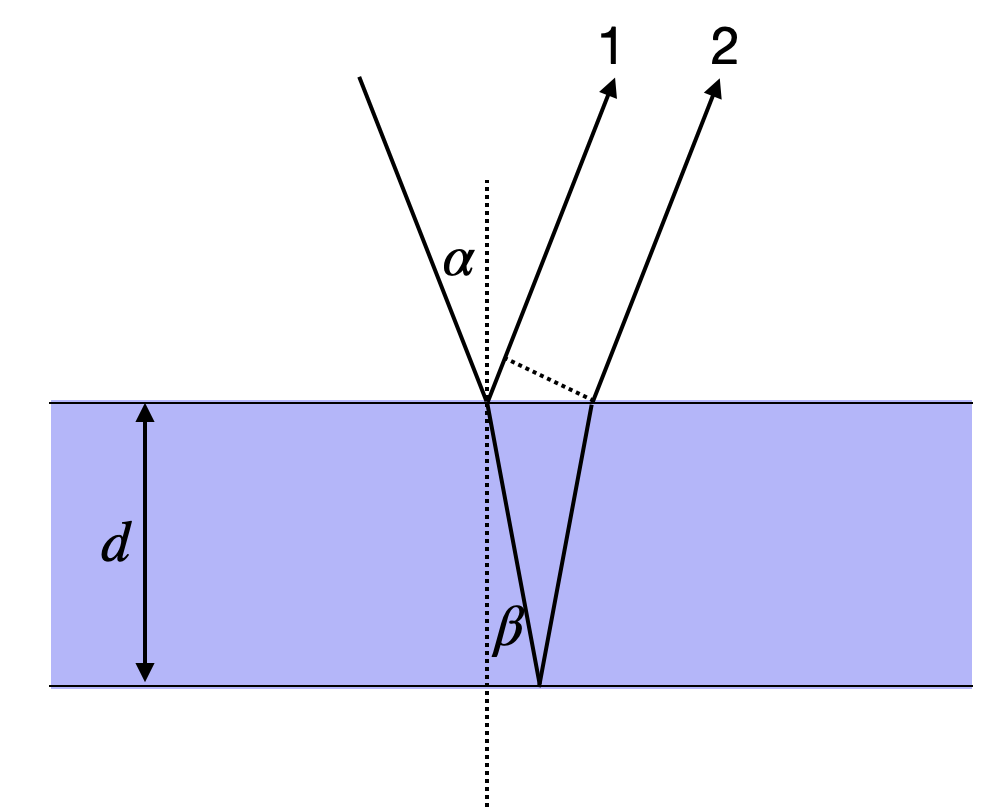
\includegraphics[width=0.5\linewidth,height=\textheight,keepaspectratio]{wave-optics/img/thin_film.png}

}

\caption{Interference on a thin film considering two partial waves.}

\end{figure}%

This picture of a single reflection at each interface is a
simplification. In reality, multiple reflections occur at both
interfaces, leading to an infinite number of partial waves. However, for
interfaces with weak reflection coefficients---such as the air-glass
interface where only about 4\% of the light is reflected---the
contribution of higher-order reflections becomes negligible. After two
reflections, the amplitude is already reduced to approximately 0.16\% of
the incident wave. Therefore, considering just the first two partial
waves provides an excellent approximation for most practical situations
involving weak reflections.

For the geometry shown in the figure above, we consider a medium with
refractive index \(n_1\) (typically air) surrounding a film with
refractive index \(n_2\). To determine when the reflected waves
interfere constructively or destructively, we must calculate the path
difference \(\Delta s\) between waves 1 and 2. This path difference
consists of two contributions: the optical path that wave 2 travels
inside the film, and the additional geometric path that wave 1 travels
after its reflection. For light incident at angle \(\alpha\) to the
normal, and refracted to angle \(\beta\) inside the film according to
Snell's law, the path difference can be expressed as:

\[
\Delta s=\frac{2n_2d}{\cos(\beta)}-2d\tan(\beta)\sin(\alpha)
\]

where \(d\) is the thickness of the film. The first term represents the
optical path inside the film traveled by wave 2, while the second term
accounts for the additional geometric path of wave 1 after reflection
(shown by the dotted line in the figure).

Using Snell's law, \(n_1\sin(\alpha) = n_2\sin(\beta)\), and setting
\(n_1 = 1\) (air) and \(n_2 = n\) (film), we can apply some
trigonometric identities to simplify this expression considerably:

\[
\Delta s =\frac{2nd}{\cos(\beta)}-\frac{2nd\sin^2(\beta)}{\cos(\beta)}=2n d \cos(\beta)=2d\sqrt{n^2-\sin^2(\alpha)}
\]

However, the optical path difference alone doesn't tell the complete
story. We must also account for phase changes that occur upon reflection
at the boundaries. The total phase difference \(\Delta \phi\) between
the waves includes both the path difference and these interface effects:

\begin{tcolorbox}[enhanced jigsaw, breakable, toptitle=1mm, bottomrule=.15mm, colbacktitle=quarto-callout-important-color!10!white, title=\textcolor{quarto-callout-important-color}{\faExclamation}\hspace{0.5em}{General Phase Difference Formula for Thin Films}, arc=.35mm, rightrule=.15mm, bottomtitle=1mm, opacityback=0, toprule=.15mm, coltitle=black, leftrule=.75mm, opacitybacktitle=0.6, colback=white, left=2mm, titlerule=0mm, colframe=quarto-callout-important-color-frame]

\[\Delta \phi=\frac{2\pi}{\lambda}\Delta s +\pi\]

where:

\begin{itemize}
\tightlist
\item
  \(\Delta s = 2d\sqrt{n^2-\sin^2(\alpha)}\) is the optical path
  difference
\item
  \(\lambda\) is the wavelength of light in vacuum
\item
  \(d\) is the film thickness
\item
  \(n\) is the refractive index of the film
\item
  \(\alpha\) is the incident angle
\item
  The additional \(\pi\) term represents the phase jump at the first
  interface (when \(n_1 < n_2\))
\end{itemize}

\textbf{Key insight:} The phase jump of \(\pi\) occurs whenever light
reflects from an optically denser medium (higher refractive index). No
phase jump occurs when reflecting from a less dense medium.

\end{tcolorbox}

The additional \(\pi\) term in the phase difference is crucial and
arises from the reflection at the first interface where \(n_1 < n_2\).
This phase jump of \(\pi\) radians (or half a wavelength in optical
path) occurs whenever light reflects from an optically denser medium. No
such phase jump occurs at the second interface where light in the film
(\(n_2\)) reflects from the surrounding medium (\(n_1 < n_2\)).

\begin{tcolorbox}[enhanced jigsaw, breakable, toptitle=1mm, bottomrule=.15mm, colbacktitle=quarto-callout-note-color!10!white, title=\textcolor{quarto-callout-note-color}{\faInfo}\hspace{0.5em}{Phase Jump at Boundaries}, arc=.35mm, rightrule=.15mm, bottomtitle=1mm, opacityback=0, toprule=.15mm, coltitle=black, leftrule=.75mm, opacitybacktitle=0.6, colback=white, left=2mm, titlerule=0mm, colframe=quarto-callout-note-color-frame]

Waves may experience phase jumps upon reflection, depending on the
relative refractive indices of the two media. A light wave will
experience a phase jump of \(\pi\) when reflecting from a medium of
higher refractive index. Conversely, no phase jump occurs when light
reflects from a medium of lower refractive index. This phenomenon is
analogous to a wave on a string: when the string is attached to a rigid
wall (like going from a less dense to a more dense medium), the
reflected wave is inverted. When the string end is free (like going from
a denser to a less dense medium), the reflected wave is not inverted.
The detailed physical reasons will be covered when we examine the
\emph{Fresnel formulas in electromagnetic optics}.

\end{tcolorbox}

\section{Normal Incidence: Simplifying the
Analysis}\label{normal-incidence-simplifying-the-analysis}

To develop intuition for thin film interference, let's consider the
simpler case of normal incidence where \(\alpha=0\). In this
configuration, light strikes the film perpendicular to its surface,
eliminating the angular dependence and simplifying the path difference
to \(\Delta s = 2nd\). The phase difference then becomes:

\begin{tcolorbox}[enhanced jigsaw, breakable, toptitle=1mm, bottomrule=.15mm, colbacktitle=quarto-callout-tip-color!10!white, title=\textcolor{quarto-callout-tip-color}{\faLightbulb}\hspace{0.5em}{Phase Difference at Normal Incidence}, arc=.35mm, rightrule=.15mm, bottomtitle=1mm, opacityback=0, toprule=.15mm, coltitle=black, leftrule=.75mm, opacitybacktitle=0.6, colback=white, left=2mm, titlerule=0mm, colframe=quarto-callout-tip-color-frame]

\[\Delta \phi=\frac{2\pi}{\lambda}2dn+\pi = \frac{4\pi nd}{\lambda}+\pi\]

This simplified formula applies when light hits the film perpendicular
to its surface (\(\alpha = 0\)).

\textbf{For constructive interference:} \(\Delta \phi = 2\pi m\) where
\(m = 1, 2, 3, ...\)

\textbf{For destructive interference:} \(\Delta \phi = \pi(2m-1)\) where
\(m = 1, 2, 3, ...\)

\end{tcolorbox}

When searching for constructive interference, the phase shift should
correspond to an integer multiple of \(2\pi\), that is,
\(\Delta \phi = 2\pi m\) where \(m\) is a positive integer. An
interesting observation emerges from this equation: for a film thickness
of \(d = 0\), we would have a residual phase shift of \(\pi\), meaning
destructive interference. While a zero-thickness film is not physically
meaningful, this tells us that very thin films will tend to suppress
reflection rather than enhance it---a fact we'll explore further when
discussing Newton black films.

There are two complementary ways to analyze thin film interference, each
useful for different applications. We can either determine what film
thickness produces constructive interference for a given wavelength
(useful for designing optical coatings), or we can determine which
wavelengths interfere constructively for a given film thickness (useful
for understanding colored patterns in soap films and oil slicks). Let's
explore both approaches through concrete examples.

\subsection{Fixed Wavelength: Designing Optical
Coatings}\label{fixed-wavelength-designing-optical-coatings}

When we fix the wavelength \(\lambda\) and solve for the film thickness
that produces constructive interference, we obtain:

\begin{tcolorbox}[enhanced jigsaw, breakable, toptitle=1mm, bottomrule=.15mm, colbacktitle=quarto-callout-important-color!10!white, title=\textcolor{quarto-callout-important-color}{\faExclamation}\hspace{0.5em}{Thickness for Constructive Interference}, arc=.35mm, rightrule=.15mm, bottomtitle=1mm, opacityback=0, toprule=.15mm, coltitle=black, leftrule=.75mm, opacitybacktitle=0.6, colback=white, left=2mm, titlerule=0mm, colframe=quarto-callout-important-color-frame]

\[d=\frac{(2m-1)\lambda}{4n}\]

where \(m = 1, 2, 3, ...\) is the order of interference.

\textbf{Minimum thickness for constructive interference:} Setting
\(m = 1\) gives \(d = \frac{\lambda}{4n}\), known as a quarter-wave
film.

\textbf{Application:} This formula is fundamental for designing
anti-reflection coatings, dichroic mirrors, and optical filters. By
choosing the appropriate thickness, we can selectively enhance or
suppress specific wavelengths.

\end{tcolorbox}

This relationship tells us that constructive interference occurs at
discrete thicknesses separated by \(\lambda/(2n)\). The thinnest film
showing constructive interference has thickness \(d = \lambda/(4n)\),
called a quarter-wave film. This principle is exploited in
anti-reflection coatings on eyeglasses, camera lenses, and solar panels,
where a carefully chosen film thickness minimizes reflections at a
target wavelength (typically green light at 550 nm, where human eyes are
most sensitive).

When we observe thin films of varying thickness, such as a soap film
stretched across a wire frame, regions of the same thickness appear as
colored fringes. These interference fringes correspond to iso-thickness
lines, providing a visual map of the film's thickness variation. This
property makes thin film interference useful for precision measurements
in optical metrology and quality control.

\subsection{Fixed Thickness: Understanding Colored
Films}\label{fixed-thickness-understanding-colored-films}

Now let's consider the complementary situation: a film of fixed
thickness \(d\) illuminated by white light containing a mixture of
wavelengths. In this case, only certain wavelengths will satisfy the
condition for constructive interference:

\begin{tcolorbox}[enhanced jigsaw, breakable, toptitle=1mm, bottomrule=.15mm, colbacktitle=quarto-callout-important-color!10!white, title=\textcolor{quarto-callout-important-color}{\faExclamation}\hspace{0.5em}{Wavelengths Showing Constructive Interference}, arc=.35mm, rightrule=.15mm, bottomtitle=1mm, opacityback=0, toprule=.15mm, coltitle=black, leftrule=.75mm, opacitybacktitle=0.6, colback=white, left=2mm, titlerule=0mm, colframe=quarto-callout-important-color-frame]

\[\lambda_{max}=\frac{4nd}{2m-1}\]

where \(m = 1, 2, 3, ...\) determines which wavelengths are enhanced.

\textbf{Key insight:} For a given thickness \(d\), only discrete
wavelengths satisfy constructive interference. The longest wavelength
(corresponding to \(m = 1\)) dominates the color we perceive.

\textbf{Why thin films appear colored:} When white light illuminates a
thin film, only specific wavelengths are strongly reflected, while
others are suppressed by destructive interference. This wavelength
selectivity creates the vivid colors in soap bubbles, oil slicks, and
butterfly wings.

\end{tcolorbox}

This equation explains why thin films appear colored when illuminated by
white light. Unlike a pigment that absorbs certain wavelengths, a thin
film selectively reflects certain wavelengths through constructive
interference while suppressing others through destructive interference.
The color we perceive depends primarily on the longest wavelength
satisfying the constructive interference condition (corresponding to
\(m = 1\)), as our eyes are most sensitive to these visible wavelengths.
Let's examine several concrete examples to understand how film thickness
determines color.

\subsubsection{Example: 100 nm Water Film --- Green
Reflection}\label{example-100-nm-water-film-green-reflection}

Consider a thin water film with thickness \(d = 100\) nm and refractive
index \(n = 1.33\) (typical for water). Applying our formula for the
wavelengths that experience constructive interference:

\[
\lambda_{max}=\frac{4\cdot 100\, {\rm nm} \cdot 1.33}{2m-1} = \frac{532\, {\rm nm}}{2m-1}
\]

For different interference orders \(m\), we find:

For \(m = 1\): \(\lambda_{max} = 532\) nm (green light in the visible
spectrum) For \(m = 2\): \(\lambda_{max} = 177\) nm (deep ultraviolet,
invisible to human eyes) For \(m = 3\): \(\lambda_{max} = 106\) nm
(extreme ultraviolet, invisible)

This calculation reveals something important: the longest wavelength
producing constructive interference is 532 nm, which falls squarely in
the green region of the visible spectrum. The next longest wavelength at
177 nm is far into the ultraviolet and completely invisible to our eyes.
Therefore, a 100 nm water film illuminated by white light will appear
green in reflected light.

The left plot in the figure below shows the intensity distribution
across wavelengths, where you can see that the green maximum is quite
broad. This means the color appears as a fairly pure green rather than a
sharp spectral line. This is actually useful for practical applications:
if you observe green light reflecting from a soap film, you can
immediately estimate that the film thickness is approximately 100 nm!
This simple observation demonstrates how thin film interference provides
a non-invasive way to measure film thickness in real-time, a technique
used in industrial coating processes and materials science research.

\begin{figure}

\centering{

\pandocbounded{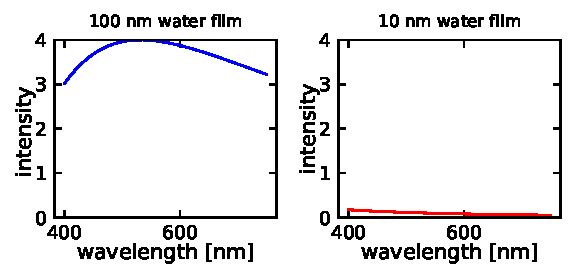
\includegraphics[keepaspectratio]{wave-optics/Thin Film Interference_files/figure-pdf/fig-reflection-output-1.pdf}}

}

\caption{\label{fig-reflection}Intensity of reflection for a 100 nm and
a 10 nm film of water.}

\end{figure}%

\subsubsection{Newton Black Films: When Thin Films
Disappear}\label{newton-black-films-when-thin-films-disappear}

A fascinating phenomenon occurs when the water film becomes extremely
thin. We might ask: at what thickness does constructive interference no
longer occur anywhere in the visible range? To answer this, we set the
shortest visible wavelength \(\lambda_{max} = 400\) nm (violet light)
and calculate the minimum film thickness needed for first-order
constructive interference (\(m = 1\)):

\[
d=\frac{(2m-1)\lambda_{max}}{4n}=\frac{\lambda_{max}}{4n} \approx 75\, {\rm nm}
\]

This tells us that for water film thicknesses below approximately 75 nm,
there is no constructive interference in the visible spectrum. The film
still reflects some light, but no particular color is enhanced. As the
film becomes even thinner, something remarkable happens: the reflected
intensity decreases further due to destructive interference. At around
10 nm thickness, as shown on the right side of the figure above, the
reflection is almost completely suppressed, and the film appears black.

These ultra-thin films are called \textbf{Newton black films}, named
after Isaac Newton who first studied them systematically. If you look
carefully at soap bubbles, you'll often see dark patches that look like
holes in the bubble surface. These aren't actually holes---the bubble
membrane is still intact---but rather regions where the film has thinned
to only a few tens of nanometers, causing the light to interfere
destructively and creating almost no reflection. Just before a soap
bubble bursts, these black regions typically expand rapidly as the film
drains and thins. The appearance of Newton black films signals that the
film has reached a thickness of only a few molecular layers,
representing one of the thinnest stable liquid films that can exist.

\subsubsection{Thick Films: Multiple Colors and White
Appearance}\label{thick-films-multiple-colors-and-white-appearance}

As the film thickness increases to \(d = 1\) μm or even \(d = 100\) μm,
the behavior changes dramatically. Now multiple wavelengths in the
visible spectrum simultaneously satisfy the constructive interference
condition for different values of \(m\). For example, with a 1 μm film,
we might have red light interfering constructively at \(m = 3\), green
at \(m = 4\), and blue at \(m = 5\). When multiple colors are reflected
with comparable intensities, the human eye perceives this as mixed
colors or even white light.

This explains an important practical observation: thin films only appear
vibrantly colored when their thickness is on the order of hundreds of
nanometers. Thicker films, such as a glass microscope slide or a layer
of plastic wrap, appear colorless in reflection despite technically
exhibiting thin film interference. The interference fringes become so
densely packed in wavelength space that our eyes cannot resolve the
individual colors, and we perceive the average as white or colorless.
The diagrams below illustrate this effect for 1 μm and 100 μm thick
water films.

\begin{figure}

\centering{

\pandocbounded{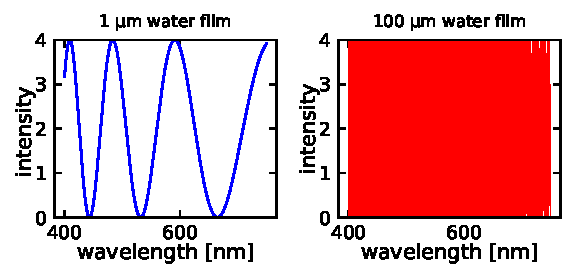
\includegraphics[keepaspectratio]{wave-optics/Thin Film Interference_files/figure-pdf/fig-reflection2-output-1.pdf}}

}

\caption{\label{fig-reflection2}Reflection from a 1µm (left) and a 100
µm (right)thin water film. Experimental demonstration of the reflection
of white light by a thin soap film.}

\end{figure}%

\begin{tcolorbox}[enhanced jigsaw, breakable, toptitle=1mm, bottomrule=.15mm, colbacktitle=quarto-callout-note-color!10!white, title=\textcolor{quarto-callout-note-color}{\faInfo}\hspace{0.5em}{Haidinger Fringes}, arc=.35mm, rightrule=.15mm, bottomtitle=1mm, opacityback=0, toprule=.15mm, coltitle=black, leftrule=.75mm, opacitybacktitle=0.6, colback=white, left=2mm, titlerule=0mm, colframe=quarto-callout-note-color-frame]

The circular interference patterns observed on a plane-parallel film are
called \textbf{Haidinger fringes}, named after Wilhelm von Haidinger who
first described them in 1849. These fringes appear when collimated light
passes through a transparent plate at near-normal incidence and are
localized at infinity (or in the focal plane of a lens). They arise from
multiple reflections between the parallel surfaces of the plate. Unlike
Newton's rings, which require curved surfaces and are localized near the
surfaces creating them, Haidinger fringes occur with parallel surfaces.
The pattern depends on the plate's thickness, its refractive index, the
angle of incidence, and the wavelength of light. These fringes are
commonly observed when viewing a uniformly thick glass plate or mica
sheet with a collimated light source and are used in optical testing and
interferometry.

\begin{figure}[H]

{\centering \pandocbounded{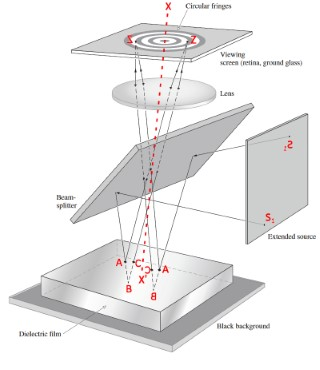
\includegraphics[keepaspectratio]{wave-optics/img/haidinger.jpg}}

}

\caption{Haidinger Fringes (c) Eugene Hecht, Optics}

\end{figure}%

\end{tcolorbox}

\section{Real-World Application: Anti-Reflection
Coatings}\label{real-world-application-anti-reflection-coatings}

One of the most important technological applications of thin film
interference is the anti-reflection coating found on eyeglasses, camera
lenses, solar panels, and telescope optics. Without such coatings, a
typical glass surface reflects about 4\% of incident light at each
air-glass interface. For a lens system with multiple elements, these
reflections accumulate, reducing image brightness, causing glare, and
creating ghost images from internal reflections.

\subsection{Design Principles of Anti-Reflection
Coatings}\label{design-principles-of-anti-reflection-coatings}

An anti-reflection coating works by exploiting destructive interference.
A thin film with carefully chosen thickness and refractive index is
deposited on the glass surface. The key design parameters are:

\begin{tcolorbox}[enhanced jigsaw, breakable, toptitle=1mm, bottomrule=.15mm, colbacktitle=quarto-callout-important-color!10!white, title=\textcolor{quarto-callout-important-color}{\faExclamation}\hspace{0.5em}{Anti-Reflection Coating Design}, arc=.35mm, rightrule=.15mm, bottomtitle=1mm, opacityback=0, toprule=.15mm, coltitle=black, leftrule=.75mm, opacitybacktitle=0.6, colback=white, left=2mm, titlerule=0mm, colframe=quarto-callout-important-color-frame]

\textbf{Refractive index:} The coating material is chosen with
\(n_{\text{coating}}\) intermediate between air and glass:
\[n_{\text{air}} < n_{\text{coating}} < n_{\text{glass}}\]

Typically: \(n_{\text{coating}} \approx 1.23\) (magnesium fluoride is a
common choice) for \(n_{\text{air}} = 1\) and
\(n_{\text{glass}} \approx 1.5\)

\textbf{Coating thickness:} Quarter-wave thickness for the target
wavelength: \[d = \frac{\lambda}{4n_{\text{coating}}}\]

where \(\lambda\) is typically around 550 nm (where the human eye is
most sensitive).

\end{tcolorbox}

\subsection{How Destructive Interference Eliminates
Reflections}\label{how-destructive-interference-eliminates-reflections}

With this quarter-wave design, the anti-reflection coating achieves
destructive interference through careful phase management:

\begin{enumerate}
\def\labelenumi{\arabic{enumi}.}
\item
  Light reflecting from the \textbf{top surface} (air-coating interface)
  undergoes a phase jump of \(\pi\) (since
  \(n_{\text{air}} < n_{\text{coating}}\))
\item
  Light traveling through the coating and reflecting from the
  \textbf{coating-glass interface} accumulates:

  \begin{itemize}
  \tightlist
  \item
    Optical path difference:
    \(2n_{\text{coating}}d = 2n_{\text{coating}} \cdot \frac{\lambda}{4n_{\text{coating}}} = \frac{\lambda}{2}\)
    → phase change of \(\pi\)
  \item
    Phase jump at reflection: \(\pi\) (since
    \(n_{\text{coating}} < n_{\text{glass}}\))
  \end{itemize}
\item
  \textbf{Total phase difference:}
  \[\Delta \phi = \pi + \pi + \pi = 3\pi \equiv \pi \pmod{2\pi}\]
\end{enumerate}

This results in destructive interference and minimal reflection at the
design wavelength.

Modern multi-layer coatings use several layers of different materials to
achieve anti-reflection over a broad wavelength range, essential for
high-performance optical systems.

\section{Soap Films and Bubbles: Nature's
Interferometers}\label{soap-films-and-bubbles-natures-interferometers}

The most beautiful and accessible examples of thin film interference are
soap bubbles and soap films. When you stretch a soap film across a wire
frame or blow a soap bubble, you're creating a dynamic interferometer
that constantly changes as gravity pulls the liquid downward, making the
film thinnest at the top and thickest at the bottom. The brilliant,
swirling colors result from interference of light reflecting off the
front and back surfaces of this thin soap membrane.

\begin{figure}

\begin{minipage}{0.50\linewidth}
\pandocbounded{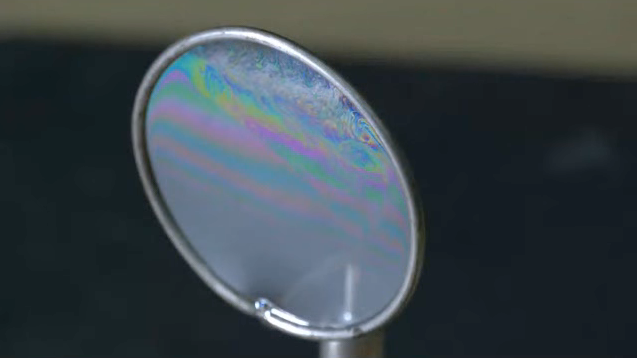
\includegraphics[keepaspectratio]{wave-optics/img/soap_film_lecture.png}}\end{minipage}%
%
\begin{minipage}{0.50\linewidth}
\pandocbounded{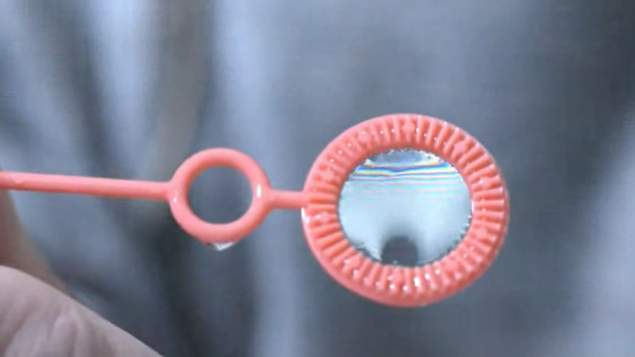
\includegraphics[keepaspectratio]{wave-optics/img/soap_film_lecture1.png}}\end{minipage}%

\caption{\label{fig-soapfilm}Experimental demonstration of the
reflection of white light by a thin soap film.}

\end{figure}%

As white light illuminates the film, different regions of different
thicknesses reflect different colors according to the constructive
interference condition we derived earlier. The top of a vertical soap
film, where it's thinnest (often less than 100 nm), may appear black
(Newton black film) or show blues and violets. Moving downward where the
film is thicker, you'll see greens, yellows, oranges, and reds in
succession. The constantly shifting patterns arise because the film is
never in equilibrium---it's continuously draining under gravity, and
convection currents create swirling flows that locally change the
thickness.

The soap film also demonstrates another important principle: the colors
you observe depend on the viewing angle. Remember that our general
formula for optical path difference includes the angle of incidence:
\(\Delta s = 2d\sqrt{n^2-\sin^2(\alpha)}\). As you change your viewing
angle relative to the film, the effective optical path through the film
changes, and different wavelengths satisfy the constructive interference
condition. This is why soap films and oil slicks shimmer with changing
colors as you move your head---you're actually changing the geometry of
the interference condition.

\section{Newton Rings: Measuring with
Interference}\label{newton-rings-measuring-with-interference}

Another classical demonstration of thin film interference produces a
pattern known as Newton's rings. This phenomenon occurs when a
hemispherical or gently curved surface is placed in contact with a flat
surface, as sketched in the image below. The air gap between the curved
and flat surfaces varies gradually with distance from the contact point,
creating a wedge-shaped thin film of air that produces circular
interference fringes.

\begin{figure}[H]

{\centering 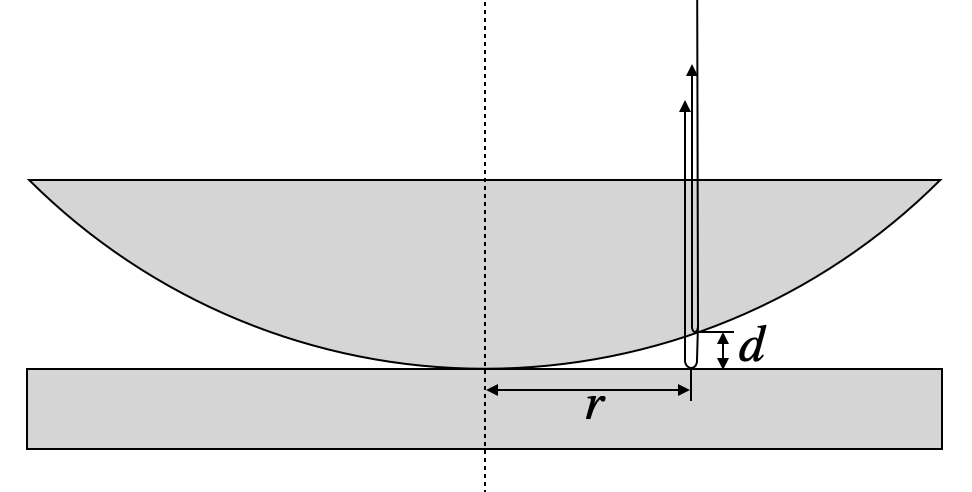
\includegraphics[width=0.8\linewidth,height=\textheight,keepaspectratio]{wave-optics/img/newton_ring_sketch.png}

}

\caption{Newton Rings. Interference of waves from a spherical and a
planar surface in close contact.}

\end{figure}%

When light is incident normal to the top surface, reflections occur at
several interfaces, but the important reflections for interference are
those at the bottom of the curved surface (reflecting from glass back
into air) and at the top of the flat surface below (reflecting from
glass, which is optically denser than air). The vertical air gap between
these surfaces is \(d\). Refraction at the curved surface does deflect
the beam slightly, but if we stay close to the axis of the spherical
surface (where \(r \ll R\), with \(R\) being the radius of curvature),
we can neglect this effect and treat the problem in terms of the simple
air gap thickness.

The path length difference between a wave reflected at the curved
surface and one reflected at the planar surface includes the round trip
through the air gap plus any phase jumps. Since the reflection at the
planar surface occurs when light in air encounters the denser glass,
there is a phase jump of \(\pi\), equivalent to an additional path
length of \(\lambda/2\):

\[
\Delta s=2d+\frac{\lambda}{2}
\]

This path difference determines where we observe bright and dark
fringes. For destructive interference (dark rings), we require:

\[
\Delta s=\frac{2m+1}{2}\lambda=2d+\frac{\lambda}{2}
\]

which simplifies to \(2d = m\lambda\) where \(m = 0, 1, 2, 3, ...\) is
an integer. Notice that at the center where the surfaces touch
(\(d = 0\), corresponding to \(m = 0\)), we observe a dark spot due to
the \(\pi\) phase jump at the lower interface. This central dark spot is
a characteristic signature of Newton's rings.

To find the radial positions of these dark rings, we need to relate the
air gap thickness \(d\) to the radial distance \(r\) from the contact
point. From the geometry of a circle with radius \(R\), we have:

\[
r^2=d(2R-d)
\]

Since the air gap is very small compared to the radius of curvature
(\(d \ll R\)), the term \(d^2\) becomes negligible compared to \(2Rd\),
allowing us to simplify to \(r^2 \approx 2dR\), which gives:

\[
d=\frac{r^2}{2R}
\]

Combining this geometric relationship with the destructive interference
condition \(2d = m\lambda\), we obtain:

\begin{tcolorbox}[enhanced jigsaw, breakable, toptitle=1mm, bottomrule=.15mm, colbacktitle=quarto-callout-important-color!10!white, title=\textcolor{quarto-callout-important-color}{\faExclamation}\hspace{0.5em}{Newton Rings Formula}, arc=.35mm, rightrule=.15mm, bottomtitle=1mm, opacityback=0, toprule=.15mm, coltitle=black, leftrule=.75mm, opacitybacktitle=0.6, colback=white, left=2mm, titlerule=0mm, colframe=quarto-callout-important-color-frame]

\[r_m=\sqrt{m\lambda R}\]

This formula gives the radius of the \(m\)-th dark ring, where:

\begin{itemize}
\tightlist
\item
  \(m = 0, 1, 2, 3, ...\) is the ring order (with \(m = 0\) at the
  center)
\item
  \(\lambda\) is the wavelength of light
\item
  \(R\) is the radius of curvature of the spherical surface
\end{itemize}

\textbf{Key insights:} - The ring radius increases with the square root
of the order number \(m\), so rings get closer together as you move
outward - Each wavelength creates its own ring pattern with different
radii - This relationship enables precise measurements: if you know
\(\lambda\), you can measure \(R\); if you know \(R\), you can measure
\(\lambda\)

\textbf{Applications:} Testing optical surfaces for flatness and
measuring radius of curvature, quality control in lens manufacturing,
precision measurements in optical metrology

\end{tcolorbox}

\begin{figure}[H]

{\centering 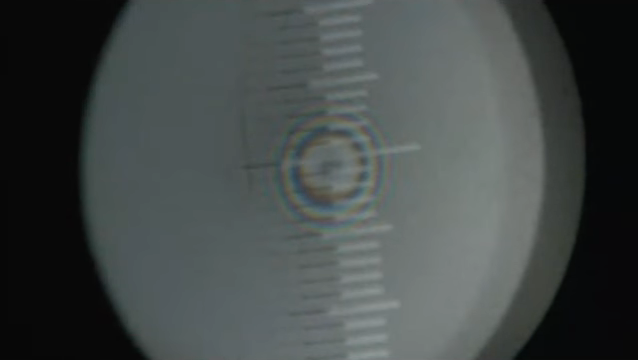
\includegraphics[width=0.8\linewidth,height=\textheight,keepaspectratio]{wave-optics/img/newton_rings_lecture.png}

}

\caption{Observation of Newton Rings using white light in the lecture.}

\end{figure}%

When using white light, as shown in the experimental image above, each
wavelength creates its own set of rings with slightly different radii
according to the formula \(r_m \propto \sqrt{\lambda}\). Since red light
has a longer wavelength than blue light, the red rings are slightly
larger, creating the beautiful colored pattern we observe. Near the
center, where the rings are widely spaced, we can distinguish individual
colors. Further out, where the rings become more closely spaced, the
colors from different wavelengths overlap more, and the pattern appears
more washed out or white.

Newton's rings provide an extraordinarily precise method for optical
measurements and quality control. By measuring the diameters of several
rings and plotting \(r_m^2\) versus \(m\), we obtain a straight line
whose slope gives \(\lambda R\). If we know the wavelength of our light
source, we can determine the radius of curvature \(R\) of the spherical
surface with high precision. Conversely, if we have a calibrated
reference sphere with known \(R\), we can measure unknown wavelengths.
The technique is also invaluable for testing optical surfaces: if a
supposedly flat surface produces non-circular rings when placed against
a reference flat, the distortion in the ring pattern directly reveals
imperfections in the surface flatness. This makes Newton's rings one of
the most sensitive methods for detecting surface irregularities as small
as a fraction of a wavelength, essential for manufacturing high-quality
telescope mirrors, laser optics, and precision optical components.

\section{Conclusion}\label{conclusion-3}

Thin film interference demonstrates the wave nature of light through the
vivid colors of soap bubbles, the practical utility of anti-reflection
coatings, and the precision measurements enabled by Newton's rings. By
understanding how optical path differences and phase jumps combine to
create constructive or destructive interference, we can both explain
natural phenomena and engineer optical devices with specific properties.
Whether designing a camera lens coating to minimize reflections,
estimating the thickness of an oil slick on water, or testing the
quality of a telescope mirror, the principles of thin film interference
provide essential tools for modern optics and photonics. The same
physics that creates the ephemeral beauty of a soap bubble also
underpins billion-dollar industries in optical coatings, photovoltaics,
and precision manufacturing.

\chapter{Multiple Wave Interference}\label{multiple-wave-interference}

So far in our study of interference, we have focused primarily on the
interaction of two waves---a useful simplification that captures the
essential physics of interference phenomena. However, this two-wave
picture is idealized. In most practical optical systems, we encounter
situations where many partial waves interfere simultaneously. Consider a
diffraction grating with thousands of parallel slits, each emitting a
wavelet that contributes to the observed pattern. Or think about light
bouncing back and forth between two highly reflective mirrors in a laser
cavity, creating hundreds of interfering reflections. These multi-wave
interference scenarios produce dramatically different and often more
useful patterns than simple two-wave interference.

Understanding multiple wave interference is crucial for explaining and
designing many important optical devices. Diffraction gratings, which we
use for spectroscopy and wavelength measurement, rely on the
interference of light from thousands of periodic sources. Fabry-Perot
interferometers, used for ultra-precise wavelength measurements and
laser frequency stabilization, exploit multiple reflections between
parallel mirrors. Even the laser itself---perhaps the most important
optical invention of the 20th century---operates through multiple wave
interference in its optical cavity. The sharp, well-defined spectral
lines produced by these devices, and their ability to resolve closely
spaced wavelengths, all stem from the physics of multiple wave
interference.

In this lecture, we will develop a general mathematical framework for
analyzing multiple wave interference. We will distinguish between two
important cases that arise in different physical situations. The first
case involves multiple waves all having the same amplitude, as occurs in
a diffraction grating where each slit contributes equally to the
interference pattern. The second case involves waves with progressively
decreasing amplitudes, as happens when light undergoes multiple
reflections in a cavity where each reflection reduces the wave
amplitude. As we'll see, these two scenarios lead to distinctly
different interference patterns with different practical applications.

\section{Multiple Wave Interference with Constant
Amplitude}\label{multiple-wave-interference-with-constant-amplitude}

Let us first consider the simpler case where multiple waves all have the
same amplitude but differ in their phase. This situation occurs, for
example, in a diffraction grating where light passes through many
equally sized slits, or in an array of coherent sources arranged
periodically. Understanding this case will provide the foundation for
analyzing more complex situations.

Consider \(M\) waves, each with the same amplitude but with successive
phase differences. The total wave amplitude is the vector sum of all
individual wave amplitudes:

\[
U=U_1+U_2+U_3+\ldots+U_M
\]

where we sum over all \(M\) partial waves. If neighboring waves (such as
\(U_1\) and \(U_2\)) have a constant phase difference \(\Delta \phi\)
due to, for example, a path length difference, then we can express the
amplitude of the \(p\)-th wave as:

\[
U_p=\sqrt{I_0}e^{i(p-1)\Delta \phi}
\]

where \(p=1,2,\ldots,M\) is an integer index, and \(\sqrt{I_0}\)
represents the amplitude of each individual wave. The total amplitude
can then be written as a geometric series:

\[
U=\sqrt{I_0}\left (1+h+h^2+\ldots +h^{M-1}\right)
\]

where we've introduced the notation \(h=e^{i\Delta \phi}\) to simplify
the expression. The beauty of recognizing this as a geometric series is
that we can immediately apply the closed-form sum formula to obtain:

\[
U=\sqrt{I_0}\frac{1-h^M}{1-h}=\sqrt{I_0}\frac{1-e^{iM\Delta \phi}}{1-e^{i\Delta \phi}}
\]

To find the observed intensity, we must calculate the squared magnitude
of this total amplitude. After factoring out appropriate phase terms and
using Euler's formula to convert complex exponentials to sines, we
arrive at a remarkably elegant result:

\begin{tcolorbox}[enhanced jigsaw, breakable, toptitle=1mm, bottomrule=.15mm, colbacktitle=quarto-callout-important-color!10!white, title=\textcolor{quarto-callout-important-color}{\faExclamation}\hspace{0.5em}{Multiple Beam Interference Formula (Equal Amplitudes)}, arc=.35mm, rightrule=.15mm, bottomtitle=1mm, opacityback=0, toprule=.15mm, coltitle=black, leftrule=.75mm, opacitybacktitle=0.6, colback=white, left=2mm, titlerule=0mm, colframe=quarto-callout-important-color-frame]

\[I=I_{0}\frac{\sin^2(M\Delta \phi/2)}{\sin^2(\Delta \phi/2)}\]

This formula describes the interference pattern from \(M\) waves of
equal amplitude with constant phase difference \(\Delta \phi\) between
neighbors.

\textbf{Key features:}

\begin{itemize}
\tightlist
\item
  \textbf{Numerator} \(\sin^2(M\Delta \phi/2)\): oscillates \(M\) times
  faster than denominator
\item
  \textbf{Denominator} \(\sin^2(\Delta \phi/2)\): creates the envelope
  of the pattern
\item
  \textbf{Maximum intensity}: \(I_{\text{max}} = M^2 I_0\) when
  \(\Delta \phi = 2\pi m\) (where \(m\) is an integer)
\item
  \textbf{First minimum}: occurs at \(\Delta \phi = 2\pi/M\)
\end{itemize}

\textbf{Physical interpretation:} As \(M\) increases, the interference
peaks become narrower and taller, while maintaining the same positions.
This sharpening is crucial for high-resolution spectroscopy.

\end{tcolorbox}

\begin{figure}

\begin{minipage}{0.50\linewidth}

\begin{figure}[H]

{\centering \pandocbounded{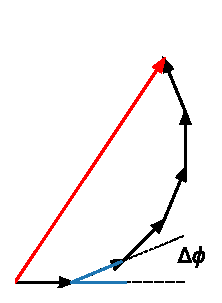
\includegraphics[keepaspectratio]{wave-optics/MultiWave Interference_files/figure-pdf/cell-3-output-1.pdf}}

}

\subcaption{Multiple wave interference of \(M=6\) waves with a phase
difference of \(\phi=\pi/8\). The black arrows represent the individual
waves, the red arrow the sum of all waves.}

\end{figure}%

\end{minipage}%
%
\begin{minipage}{0.50\linewidth}

\begin{figure}[H]

\centering{

\pandocbounded{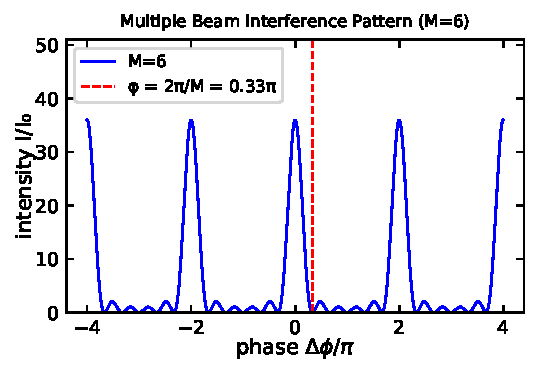
\includegraphics[keepaspectratio]{wave-optics/MultiWave Interference_files/figure-pdf/fig-multibeam2-output-1.pdf}}

}

\caption{\label{fig-multibeam2}Multiple beam interference pattern for
M=6 beams. The intensity distribution is shown as a function of the
phase shift \(\phi\). The first minimum is at \(\phi=2\pi/M\). The
intensity distribution is symmetric around \(\phi=0\).}

\end{figure}%

\end{minipage}%

\end{figure}%

This intensity formula reveals several fascinating features. The
numerator \(\sin^2(M\Delta \phi/2)\) oscillates with a frequency that is
\(M\) times higher than the denominator \(\sin^2(\Delta \phi/2)\). This
creates a rapidly oscillating pattern that produces sharp interference
peaks separated by regions of low intensity. The first minimum of the
interference peak occurs at \(\Delta \phi = 2\pi/M\), which is a crucial
result: it shows that the number of sources \(M\) directly determines
how narrow the interference peak becomes. As we add more sources, the
peaks become increasingly sharp and well-defined.

This narrowing effect has profound practical implications. In a
diffraction grating with spacing \(d\) between adjacent slits, the phase
difference between neighboring sources is
\(\Delta \phi = 2\pi d \sin(\theta)/\lambda\), just as in the
double-slit experiment. Using this relationship, we can express the
angular width of the interference peak. The first minimum occurs at an
angle given by:

\[
\sin(\theta_{\text{min}}) = \frac{\lambda}{Md}
\]

Notice that this angular width is inversely proportional to the total
width of the grating (\(Md\)), not just to the slit spacing \(d\). A
grating with 10,000 slits produces peaks that are 10,000 times narrower
than a double-slit with the same spacing! This is why diffraction
gratings can resolve spectral lines that are extremely close in
wavelength---a capability essential for spectroscopy in chemistry,
astronomy, and materials science.

A mathematically subtle but physically important situation arises when
both the numerator and denominator simultaneously approach zero. This
occurs whenever the phase difference is an integer multiple of \(2\pi\):

\[
\Delta \phi = 2\pi m
\]

where \(m\) is an integer called the interference order, representing
how many wavelengths of path difference exist between neighboring
partial waves. At these special points, our formula appears to give the
indeterminate form \(0/0\). However, applying L'Hôpital's rule or using
the small-angle approximation for the sine functions reveals that:

\[
I(\Delta \phi = 2\pi m) = M^2 I_0
\]

This is the maximum possible intensity, and it's proportional to the
square of the number of sources. This quadratic scaling is remarkable:
doubling the number of sources quadruples the peak intensity. This
explains why diffraction gratings with many lines are so much brighter
and more efficient than simple double slits. :::

\begin{figure}

\centering{

\pandocbounded{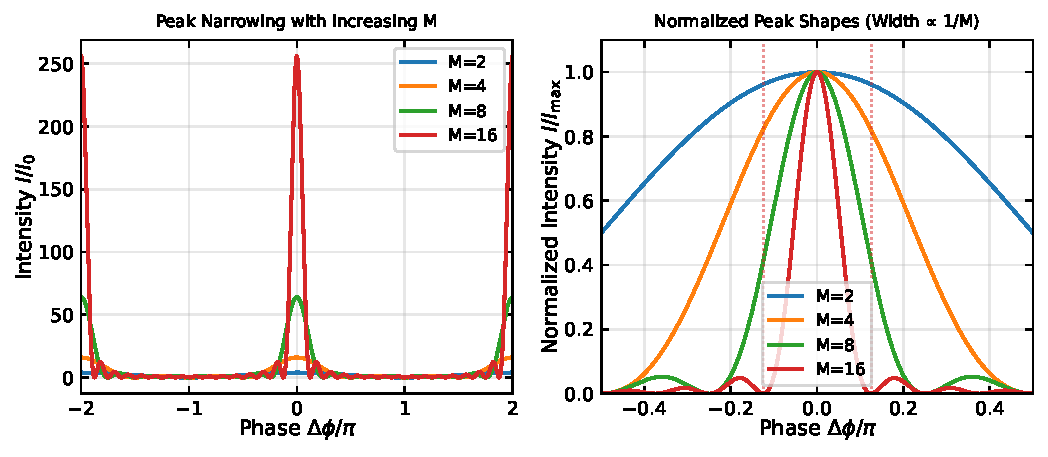
\includegraphics[keepaspectratio]{wave-optics/MultiWave Interference_files/figure-pdf/fig-peak-narrowing-output-1.pdf}}

}

\caption{\label{fig-peak-narrowing}Comparison of interference patterns
for different numbers of sources M. As M increases, the peaks become
narrower and taller while maintaining the same position. This
demonstrates the fundamental principle underlying diffraction grating
spectroscopy.}

\end{figure}%

\subsection{Application: Diffraction
Gratings}\label{application-diffraction-gratings}

The multiple beam interference formula we've derived provides the
theoretical foundation for one of the most important optical
instruments: the diffraction grating. A diffraction grating consists of
many parallel slits or lines (typically thousands) with regular spacing
\(d\). When illuminated by light, each slit acts as a coherent source,
and the interference of light from all these sources creates sharp,
bright spectral lines at specific angles determined by the wavelength
through the grating equation \(\sin(\theta_m) = m\lambda/d\).

The key result from our interference analysis is that the angular width
of each spectral peak is inversely proportional to the total number of
illuminated grating lines \(M\). This leads to the resolving power
\(R = mM\), where \(m\) is the diffraction order. More slits create
sharper peaks, enabling better separation of closely spaced
wavelengths---the fundamental principle of spectroscopic analysis.

\begin{tcolorbox}[enhanced jigsaw, breakable, toptitle=1mm, bottomrule=.15mm, colbacktitle=quarto-callout-note-color!10!white, title=\textcolor{quarto-callout-note-color}{\faInfo}\hspace{0.5em}{Further Study: Diffraction Gratings}, arc=.35mm, rightrule=.15mm, bottomtitle=1mm, opacityback=0, toprule=.15mm, coltitle=black, leftrule=.75mm, opacitybacktitle=0.6, colback=white, left=2mm, titlerule=0mm, colframe=quarto-callout-note-color-frame]

The detailed physics of diffraction gratings, including the combined
effects of single-slit diffraction and multi-slit interference, is
covered in a dedicated lecture after we study diffraction. Topics
include:

\begin{itemize}
\tightlist
\item
  Complete grating equation including diffraction envelope
\item
  Spectral resolution and resolving power
\item
  Influence of slit width and number on the diffraction pattern
\item
  Practical applications in spectroscopy and optical instruments
\item
  Real experimental observations and design considerations
\end{itemize}

The interference theory developed here provides the foundation for
understanding how gratings create their characteristic sharp spectral
lines.

\end{tcolorbox}

\subsection{Wavevector Representation: A Powerful Geometric
Insight}\label{wavevector-representation-a-powerful-geometric-insight}

There is an elegant geometric way to understand multiple wave
interference using wavevectors that provides deep insight into the
physics and connects to many other phenomena in optics and solid-state
physics. Let's rewrite the first-order (\(m=1\)) constructive
interference condition in terms of wavevectors rather than wavelengths
and angles.

The standard grating equation \(d\sin\theta = \lambda\) can be rewritten
by dividing both sides by the wavelength:

\[
\frac{1}{\lambda}\sin{\theta}= \frac{1}{d}
\]

Multiplying both sides by \(2\pi\) gives:

\[
\frac{2\pi}{\lambda}\sin{\theta}= \frac{2\pi}{d}
\]

\begin{tcolorbox}[enhanced jigsaw, breakable, toptitle=1mm, bottomrule=.15mm, colbacktitle=quarto-callout-tip-color!10!white, title=\textcolor{quarto-callout-tip-color}{\faLightbulb}\hspace{0.5em}{Wavevector Formulation of Grating Equation}, arc=.35mm, rightrule=.15mm, bottomtitle=1mm, opacityback=0, toprule=.15mm, coltitle=black, leftrule=.75mm, opacitybacktitle=0.6, colback=white, left=2mm, titlerule=0mm, colframe=quarto-callout-tip-color-frame]

\[k \sin{\theta}= K\]

where:

\begin{itemize}
\tightlist
\item
  \(k = 2\pi/\lambda\) is the magnitude of the wavevector of the light
\item
  \(K = 2\pi/d\) is the grating wavevector corresponding to the grating
  period \(d\)
\item
  \(\theta\) is the diffraction angle
\end{itemize}

\textbf{Geometric interpretation:} The grating provides momentum
transfer \(K\) to redirect the incident light. The wavevectors of
incident and diffracted light, together with the grating vector, form a
closed triangle---a vector addition
\(\vec{k}_{\text{incident}} + \vec{K} = \vec{k}_{\text{diffracted}}\).

\textbf{Universal principle:} This wavevector picture applies to X-ray
diffraction from crystals, electron diffraction, neutron scattering, and
phonon interactions---wherever periodic structures interact with waves.

\end{tcolorbox}

Since the magnitude of the light's wavevector is conserved (elastic
scattering), the incident and diffracted wavevectors both have magnitude
\(k\). Together with the grating vector \(K\), they form an isosceles
triangle, as shown in the figure below. This geometric picture reveals
that the grating is effectively providing a ``momentum kick'' of
magnitude \(K\) to change the light's direction. This same wavevector
conservation principle appears throughout physics: in X-ray diffraction
from crystals (the Bragg condition), in electron diffraction, in the
scattering of light by acoustic waves, and even in nonlinear optics
where photons combine or split.

\begin{figure}[H]

{\centering \pandocbounded{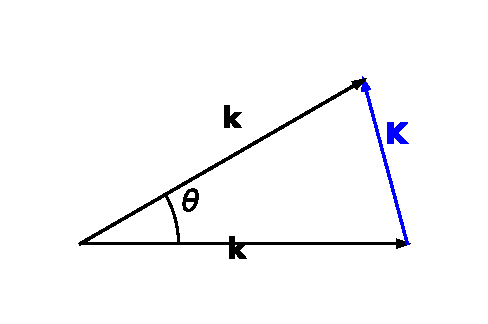
\includegraphics[keepaspectratio]{wave-optics/MultiWave Interference_files/figure-pdf/cell-7-output-1.pdf}}

}

\caption{Wavevector summation for the diffraction grating. The
wavevector of the incident light \(k\) and the wavevector of the light
traveling along the direction of the first interference peak \(K\) form
an equilateral triangle.}

\end{figure}%

This means that the diffraction grating is providing a wavevector \(K\)
to alter the direction of the incident light. This is again a common
feature reappearing in many situations as for example in the X-ray
diffraction of crystals.

\section{Multiple Wave Interference with Decreasing
Amplitude}\label{multiple-wave-interference-with-decreasing-amplitude}

We now turn our attention to a physically important variation of
multiple wave interference: the case where successive waves have
progressively decreasing amplitudes. This scenario arises naturally
whenever light undergoes multiple reflections in an optical cavity, such
as in a Fabry-Perot interferometer or the mirrors of a laser cavity.
Each time light reflects from a partially reflective surface, only a
fraction of the amplitude is reflected---the rest is transmitted through
the surface and lost from the interference pattern within the cavity.

Consider a sequence of waves where the first wave has amplitude
\(U_1 = \sqrt{I_0}\), but each subsequent wave has its amplitude reduced
by a constant factor. We express the second wave as:

\[
U_2=h U_1
\]

where \(h = re^{i\Delta\phi}\) with \(|h| = r < 1\). Here \(r\)
represents the reflection coefficient, a dimensionless number less than
one that describes what fraction of the wave amplitude survives each
reflection. The phase factor \(e^{i\Delta\phi}\) accounts for the
additional optical path traveled between successive reflections. When we
calculate the intensity of this second wave, we find:

\[
I_2=|U_2|^2=|h U_1|^2=r^2 I_1
\]

This reveals an important distinction: while the amplitude is multiplied
by \(r\) at each reflection, the intensity is multiplied by \(r^2\). The
phase factor \(e^{i\Delta\phi}\) vanishes when we take the squared
magnitude to find intensity, as \(|e^{i\Delta\phi}|^2 = 1\). This means
the phase affects where the waves interfere, but the factor \(r\)
determines how quickly the wave amplitudes decay with successive
reflections.

\begin{tcolorbox}[enhanced jigsaw, breakable, toptitle=1mm, bottomrule=.15mm, colbacktitle=quarto-callout-note-color!10!white, title=\textcolor{quarto-callout-note-color}{\faInfo}\hspace{0.5em}{Reflectance, Transmittance, and Energy Conservation}, arc=.35mm, rightrule=.15mm, bottomtitle=1mm, opacityback=0, toprule=.15mm, coltitle=black, leftrule=.75mm, opacitybacktitle=0.6, colback=white, left=2mm, titlerule=0mm, colframe=quarto-callout-note-color-frame]

The amplitude reflection coefficient \(r \le 1\) determines what
fraction of the wave amplitude is reflected at a boundary. The
corresponding \textbf{reflectance} \(R = |r|^2 \le 1\) gives the
fraction of intensity (energy per unit area per unit time) that is
reflected.

The \textbf{transmittance} \(T\) is the fraction of intensity
transmitted through the boundary. In the absence of absorption, energy
conservation requires:

\[
R+T=1
\]

\textbf{Example:} A typical uncoated glass surface has
\(R \approx 0.04\) (4\% reflectance) and \(T \approx 0.96\) (96\%
transmittance). High-quality mirror coatings can achieve \(R > 0.999\)
(99.9\% reflectance).

\textbf{Forward reference:} The Airy function and concepts of finesse
developed here form the theoretical foundation for understanding
Fabry-Perot interferometers, which are covered in detail in a separate
dedicated lecture on Fabry-Perot interferometry.

\end{tcolorbox}

Following this pattern, the third wave has amplitude
\(U_3 = hU_2 = h^2U_1\), the fourth has \(U_4 = h^3U_1\), and so on. If
we sum over many such reflections (potentially infinite in number), the
total amplitude becomes:

\[
U=U_1+U_2+U_3+\ldots = \sqrt{I_0}(1+h+h^2+\ldots)
\]

\begin{figure}

\begin{minipage}{0.50\linewidth}

\begin{figure}[H]

{\centering \pandocbounded{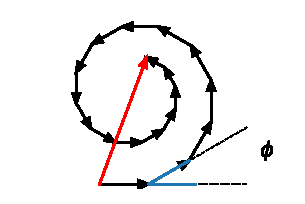
\includegraphics[keepaspectratio]{wave-optics/MultiWave Interference_files/figure-pdf/cell-8-output-1.pdf}}

}

\subcaption{Phase construction of a multiwave intereference with M waves
with decreasing amplitude due to a reflection coefficient \(r=0.95\).}

\end{figure}%

\end{minipage}%
%
\begin{minipage}{0.50\linewidth}

\begin{figure}[H]

{\centering \pandocbounded{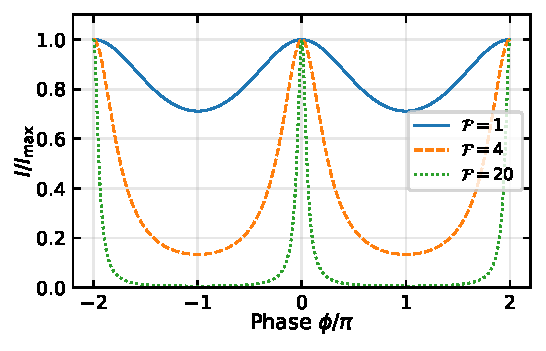
\includegraphics[keepaspectratio]{wave-optics/MultiWave Interference_files/figure-pdf/cell-9-output-1.pdf}}

}

\subcaption{Multiple wave interference with decreasing amplitude. The
graph shows the intensity distribution over the phase angle \(\phi\) for
different values of the Finesse \(\mathcal{F}\).}

\end{figure}%

\end{minipage}%

\end{figure}%

This is again a geometric series, which we can sum using the standard
formula (taking the limit as \(M \to \infty\) since reflections continue
indefinitely):

\[
U=\sqrt{I_0}\lim_{M\to\infty}\frac{(1-h^M)}{1-h}=\frac{\sqrt{I_0}}{1-r e^{i\Delta\phi}}
\]

The intensity is found by calculating \(I = |U|^2\), which requires
evaluating the squared magnitude of the complex denominator:

\[
I=|U|^2=\frac{I_{0}}{|1-re^{i\Delta\phi}|^2}=\frac{I_0}{(1-r)^2+4r\sin^2(\Delta\phi/2)}
\]

This fundamental result is known as the \textbf{Airy function} or Airy
formula, named after the British astronomer George Biddell Airy who
first derived it in 1833 while studying the properties of spectroscopic
instruments.

\begin{tcolorbox}[enhanced jigsaw, breakable, toptitle=1mm, bottomrule=.15mm, colbacktitle=quarto-callout-important-color!10!white, title=\textcolor{quarto-callout-important-color}{\faExclamation}\hspace{0.5em}{Airy Function: Multiple Reflections with Losses}, arc=.35mm, rightrule=.15mm, bottomtitle=1mm, opacityback=0, toprule=.15mm, coltitle=black, leftrule=.75mm, opacitybacktitle=0.6, colback=white, left=2mm, titlerule=0mm, colframe=quarto-callout-important-color-frame]

\[I=\frac{I_{\rm max}}{1+4\left(\frac{\mathcal{F}}{\pi}\right)^2\sin^{2}(\Delta\phi/2)}\]

where: - \(I_{\rm max}=\frac{I_0}{(1-r)^2}\) is the maximum transmitted
intensity - \(\mathcal{F}=\frac{\pi \sqrt{r}}{1-r}\) is the
\textbf{finesse}, a dimensionless quality factor - \(\Delta\phi\) is the
round-trip phase accumulated in the cavity

\textbf{Key features:}

\begin{itemize}
\tightlist
\item
  \textbf{Peak sharpness} increases dramatically with finesse
  \(\mathcal{F}\)
\item
  \textbf{High reflectivity} (\(r \to 1\)) gives high finesse and very
  narrow peaks
\item
  \textbf{Maximum intensity} occurs when \(\Delta\phi = 2\pi m\)
  (constructive interference)
\item
  \textbf{Between peaks}, transmission drops to nearly zero for high
  finesse
\end{itemize}

\textbf{Applications:} Fabry-Perot interferometers, laser cavities,
optical filters, wavelength meters

\end{tcolorbox}

The finesse \(\mathcal{F}\) is perhaps the most important parameter
characterizing a Fabry-Perot cavity or any resonant optical system. It
quantifies how ``sharp'' the resonance peaks are compared to their
spacing. A cavity with highly reflective mirrors (say \(r = 0.99\),
giving \(R = 98\%\) reflectance) has a finesse of about
\(\mathcal{F} \approx 310\), producing extremely narrow transmission
peaks. This makes such cavities exquisitely sensitive to small changes
in wavelength or cavity length.

The intensity distribution described by the Airy function has a
profoundly different character from the equal-amplitude case. As we
increase the finesse, the intensity maxima---which occur at multiples of
\(2\pi\) in phase---become dramatically narrower and more isolated.
Between the maxima, the intensity drops to nearly zero, creating regions
of almost complete destructive interference. This sharp wavelength
selectivity makes Fabry-Perot interferometers indispensable for
applications requiring ultra-high spectral resolution, such as measuring
the frequency stability of lasers, detecting tiny Doppler shifts in
astrophysics, and studying the fine structure of atomic emission lines.

\section{Connection to Fabry-Perot
Interferometry}\label{connection-to-fabry-perot-interferometry}

The Airy function we've derived is the fundamental intensity
distribution for any optical system involving multiple reflections with
decreasing amplitude. The most important practical realization of this
physics is the \textbf{Fabry-Perot interferometer}, which consists of
two parallel, partially reflective mirrors separated by a distance
\(L\). When light enters this cavity, it bounces back and forth many
times, with each reflection reducing the amplitude by the factor \(r\),
creating exactly the scenario we've analyzed.

The Fabry-Perot interferometer exhibits transmission peaks whenever the
round-trip phase satisfies \(\Delta\phi = 4\pi L/\lambda = 2\pi m\),
corresponding to cavity lengths that are integer multiples of
half-wavelengths. The sharpness of these peaks---characterized by the
finesse---makes Fabry-Perot devices essential for applications requiring
ultra-high spectral resolution, such as laser frequency stabilization,
precision spectroscopy, and optical communications.

\begin{tcolorbox}[enhanced jigsaw, breakable, toptitle=1mm, bottomrule=.15mm, colbacktitle=quarto-callout-note-color!10!white, title=\textcolor{quarto-callout-note-color}{\faInfo}\hspace{0.5em}{Further Study: Fabry-Perot Interferometers}, arc=.35mm, rightrule=.15mm, bottomtitle=1mm, opacityback=0, toprule=.15mm, coltitle=black, leftrule=.75mm, opacitybacktitle=0.6, colback=white, left=2mm, titlerule=0mm, colframe=quarto-callout-note-color-frame]

The detailed physics, applications, and experimental techniques of
Fabry-Perot interferometry are covered in a dedicated lecture. Topics
include:

\begin{itemize}
\tightlist
\item
  Free spectral range and spectral resolution
\item
  Ring pattern formation and interpretation
\item
  Applications in spectroscopy, laser technology, and optical
  communications
\item
  Modern implementations in photonics and quantum optics
\end{itemize}

The Airy function and finesse concepts developed here provide the
theoretical foundation for understanding these practical devices.

\end{tcolorbox}

\begin{figure}

\centering{

\pandocbounded{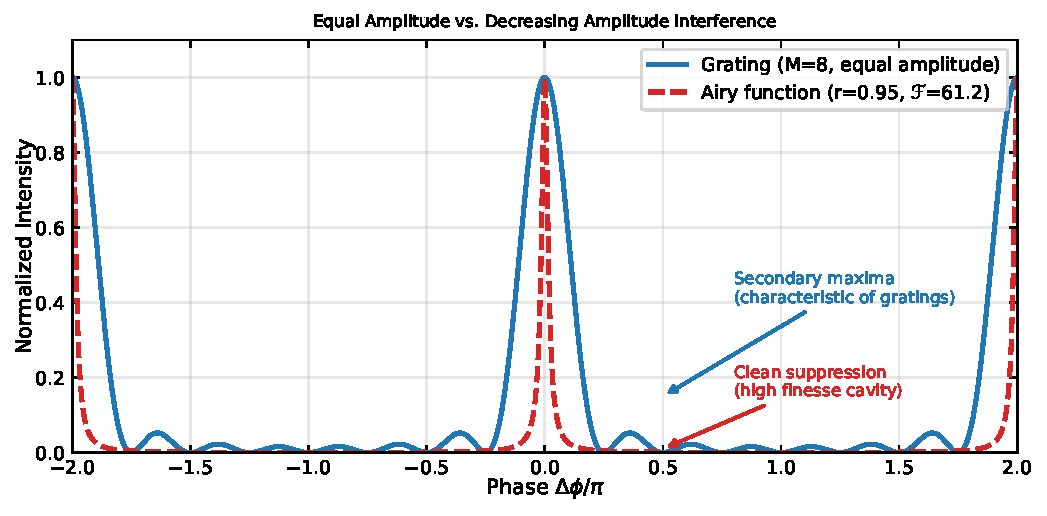
\includegraphics[keepaspectratio]{wave-optics/MultiWave Interference_files/figure-pdf/fig-grating-vs-fabry-output-1.pdf}}

}

\caption{\label{fig-grating-vs-fabry}Comparison between equal-amplitude
interference (diffraction grating, blue) and decreasing-amplitude
interference (Airy function with high finesse, red). The grating shows
secondary maxima between main peaks, while the Airy function shows clean
suppression between resonances - a key distinction exploited in
Fabry-Perot interferometers.}

\end{figure}%

\section{Conclusion: From Fundamental Physics to Precision
Technology}\label{conclusion-from-fundamental-physics-to-precision-technology}

The transition from two-wave to multiple-wave interference represents
more than just mathematical generalization---it reveals a profound
principle that underpins much of modern photonics. When many coherent
sources interfere, whether they have equal amplitudes (as in diffraction
gratings) or decreasing amplitudes (as in Fabry-Perot cavities and laser
resonators), the resulting patterns exhibit dramatically sharper
features than simple two-wave interference. This sharpening effect,
characterized mathematically by the \(M^2\) intensity scaling in
gratings and the finesse parameter in the Airy function, provides the
foundation for optical instruments of extraordinary precision and
capability.

\textbf{Diffraction gratings}, exploiting the equal-amplitude
interference of thousands of sources, have become indispensable tools
for separating and analyzing light. As we'll explore in detail in the
dedicated lecture on diffraction gratings, these devices combine the
interference principles developed here with single-slit diffraction
effects to create powerful spectroscopic instruments used throughout
science and technology---from astronomical spectroscopy revealing the
composition of distant stars to compact spectrometers in chemistry labs
and wavelength-division multiplexing in optical communications.

The Airy function, describing interference with decreasing amplitudes,
governs systems where waves undergo multiple reflections in optical
cavities. As we'll see in the dedicated lecture on \textbf{Fabry-Perot
interferometry}, this physics enables wavelength measurements accurate
to parts per billion, frequency stabilization of lasers to better than
one part in \(10^{15}\), and spectroscopic resolution sufficient to
observe individual spectral components separated by only megahertz. The
remarkably narrow transmission peaks of high-finesse cavities make
Fabry-Perot devices essential for applications ranging from laser
technology and precision spectroscopy to optical communications and
quantum optics.

The mathematical frameworks we've developed---the multi-beam formula for
equal amplitudes and the Airy function for decreasing
amplitudes---appear throughout physics wherever periodic structures
interact with waves. The same wavevector addition that describes grating
diffraction also governs X-ray scattering from crystal lattices (Bragg
diffraction), the electronic band structure of semiconductors, and even
the propagation of light in photonic crystals that act as
``semiconductors for photons.'' Understanding multiple wave interference
thus provides not just isolated techniques for optical measurements, but
a universal language for describing how waves interact with periodic
structures across all scales and all branches of physics.

\chapter{Fabry Perot Interferometer}\label{fabry-perot-interferometer}

The Fabry-Perot interferometer demonstrates multiple-wave interference
with decreasing amplitude. It consists of two parallel mirrors separated
by a distance \(d\), creating multiple reflections of incident light.

\begin{figure}[H]

{\centering 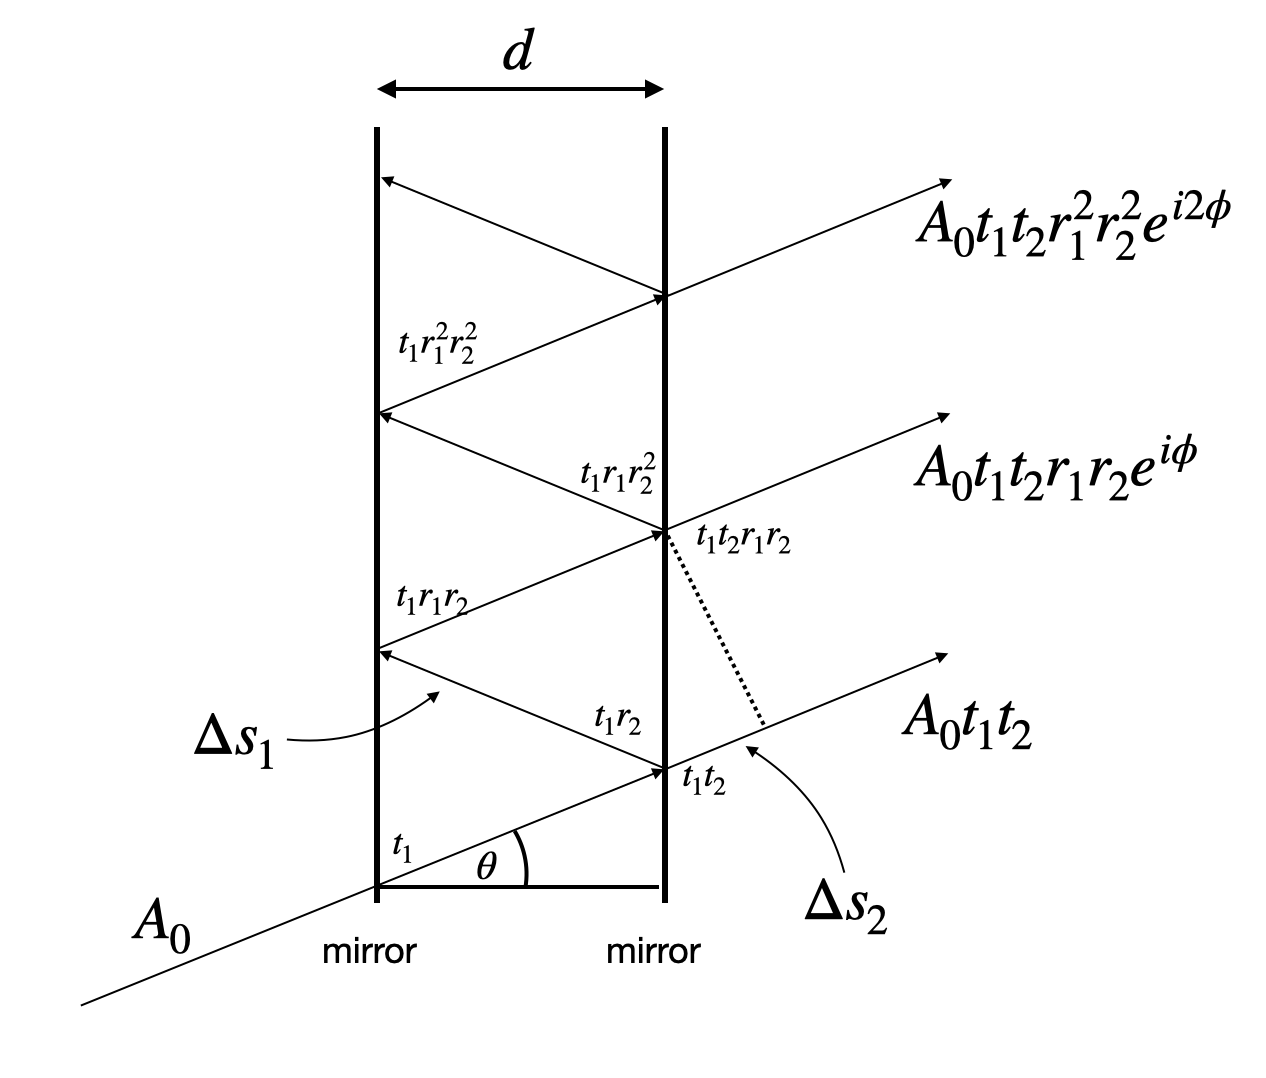
\includegraphics[width=0.7\linewidth,height=\textheight,keepaspectratio]{wave-optics/img/fabry_perot.png}

}

\caption{Simplified Sketch of a Fabry-Perot Interferometer.}

\end{figure}%

When light with amplitude \(A_0\) enters the interferometer, it
undergoes a series of transmissions and reflections. The first
transmitted wave has amplitude:

\[
U_1=A_0t_1 t_2
\]

where \(t_1\) and \(t_2\) are the transmission coefficients of the first
and second mirrors. The second transmitted wave includes reflections
from both mirrors (\(r_1\) and \(r_2\)) and a phase shift
\(\Delta\phi\):

\[
U_2=A_0t_1 t_2 r_1 r_2 e^{i\phi}=U_1 r_1 r_2 e^{i\Delta\phi}
\]

This follows our earlier treatment of multiple-wave interference with
decreasing amplitude, where \(\sqrt{I_0}=A_0 t_1 t_2\) and \(r=r_1r_2\).
The phase shift between successive reflections is:

\[
\phi=\frac{2\pi}{\lambda} \Delta s = \frac{2\pi}{\lambda} 2d\cos(\theta)
\]

where \(\Delta s=2d\cos(\theta)\) represents the path difference between
adjacent rays.

The resulting intensity distribution is:

\[
I=|U|^2=\frac{I_{0}}{|1-re^{i\phi}|^2}=\frac{I_0}{(1-r)^2+4r\sin^2\left (\frac{2\pi}{\lambda} d\cos(\theta)\right)}
\]

\begin{figure}[H]

{\centering 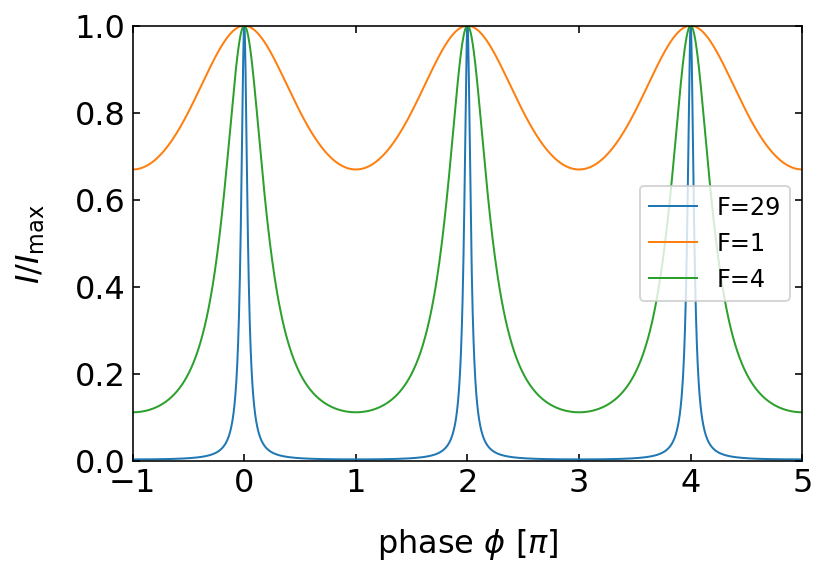
\includegraphics[width=0.6\linewidth,height=\textheight,keepaspectratio]{wave-optics/img/perot.png}

}

\caption{Fabry Perot Interferometer.}

\end{figure}%

\subsection{Finesse and Spectral
Properties}\label{finesse-and-spectral-properties}

The quality of interference in a Fabry-Perot interferometer is
characterized by the Finesse \(\mathcal{F}\):

\[
\mathcal{F}=\frac{\pi \sqrt{r}}{1-r}
\]

where \(r=r_1r_2\) is the product of the mirrors' reflection
coefficients. As \(r\) approaches 1 (higher reflectivity), the Finesse
increases, resulting in sharper interference peaks.

For normal incidence (\(\theta=0\)), the phase difference simplifies to:

\[
\Delta\phi=\frac{4\pi d}{\lambda}
\]

Constructive interference occurs when \(\Delta\phi=m2\pi\) (where \(m\)
is an integer), giving us the wavelengths of transmission maxima:

\[
\lambda_m=\frac{2d}{m}
\]

\subsubsection{Free Spectral Range}\label{free-spectral-range}

The spacing between adjacent transmission peaks in an optical system can
be expressed in terms of either wavelength or frequency. This spacing is
known as the \textbf{free spectral range (FSR)}.

\textbf{In Wavelength:}

The difference in wavelength between adjacent transmission peaks is
given by:

\[
   \delta \lambda = \lambda_{m} - \lambda_{m+1} = \frac{\lambda_m}{m+1}
   \]

Here, \(\lambda_m\) is the wavelength corresponding to the \(m\)-th
transmission peak.

\textbf{In Frequency:}

The difference in frequency between adjacent transmission peaks is given
by:

\[
   \delta \nu = \nu_{m+1} - \nu_m = \frac{c}{2d}
   \]

Here, \(c\) is the speed of light, and \(d\) is the distance between the
reflecting surfaces in the optical system.

The free spectral range (FSR) represents the interval between successive
transmission peaks and is a crucial parameter in the design and analysis
of optical systems, such as Fabry-Pérot interferometers and optical
resonators.

\subsubsection{Spectral Resolution}\label{spectral-resolution}

The spectral resolution of an interferometer is determined by the width
of its interference peaks, which indicates the instrument's ability to
distinguish between closely spaced wavelengths. This width is often
characterized by the full width at half maximum (FWHM) of the peaks.

To find the FWHM, we start with the intensity ratio at half maximum:

\[
\frac{I}{I_{\rm max}} = \frac{1}{2} = \frac{1}{1 + \left( \frac{\mathcal{F}}{\pi} \right)^2 \Delta \phi_{1/2}^2 }
\]

Solving for the phase difference \(\Delta \phi_{1/2}\) at half maximum,
we can determine the corresponding frequency width:

\[
\Delta \nu = \frac{c}{2d \mathcal{F}} = \frac{\delta \nu}{\mathcal{F}}
\]

Here, \(\delta \nu\) is the free spectral range, \(c\) is the speed of
light, \(d\) is the distance between the reflecting surfaces, and
\(\mathcal{F}\) is the finesse of the interferometer.

The finesse \(\mathcal{F}\) is defined as the ratio of the free spectral
range to the FWHM:

\[
\mathcal{F} = \frac{\delta \nu}{\Delta \nu} = \frac{\lambda}{\Delta \lambda}
\]

This ratio provides a measure of the interferometer's spectral
resolution, indicating how well it can separate two closely spaced
spectral lines.

The overall resolving power \(\mathcal{R}\) of the interferometer is
given by:

\[
\mathcal{R} = m \mathcal{F}
\]

where \(m\) is the order of the interference. The resolving power
\(\mathcal{R}\) quantifies the ability of the interferometer to resolve
spectral features, with higher values indicating better resolution.

\begin{figure}[H]

{\centering 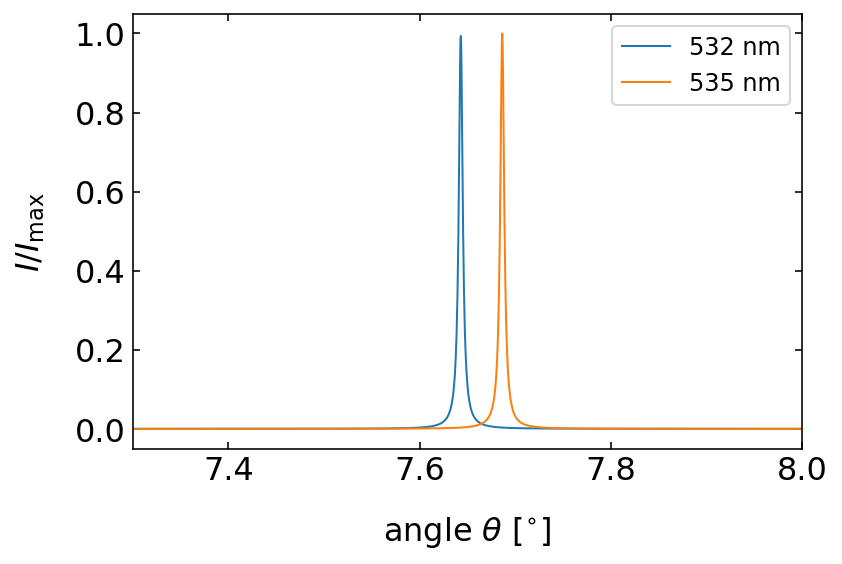
\includegraphics[width=0.6\linewidth,height=\textheight,keepaspectratio]{wave-optics/img/perot_spectral.png}

}

\caption{Two different wavelengths interfering constructively in a Fabry
Perot interferometer.}

\end{figure}%

\begin{tcolorbox}[enhanced jigsaw, breakable, toptitle=1mm, bottomrule=.15mm, colbacktitle=quarto-callout-note-color!10!white, title=\textcolor{quarto-callout-note-color}{\faInfo}\hspace{0.5em}{Free Spectral Range and Spectral Resolution}, arc=.35mm, rightrule=.15mm, bottomtitle=1mm, opacityback=0, toprule=.15mm, coltitle=black, leftrule=.75mm, opacitybacktitle=0.6, colback=white, left=2mm, titlerule=0mm, colframe=quarto-callout-note-color-frame]

\textbf{Free Spectral Range (FSR):}

The free spectral range is the spacing between adjacent transmission
maxima in a Fabry-Perot interferometer. It can be expressed in terms of
wavelength or frequency:

\begin{itemize}
\item
  In wavelength: \[
  \delta \lambda = \lambda_{m} - \lambda_{m+1} = \frac{\lambda_m}{m+1}
  \]
\item
  In frequency: \[
  \delta \nu = \nu_{m+1} - \nu_m = \frac{c}{2d}
  \]
\end{itemize}

The FSR indicates the range over which the interferometer can
distinguish between different wavelengths or frequencies before the next
order of interference occurs.

\textbf{Spectral Resolution:}

The spectral resolution of a Fabry-Perot interferometer is determined by
the width of the interference peaks. It is often quantified by the
Finesse (\(\mathcal{F}\)), which is the ratio of the free spectral range
to the full width at half maximum (FWHM) of the peaks:

\[
\mathcal{F} = \frac{\delta \nu}{\Delta \nu} = \frac{\lambda}{\Delta \lambda}
\]

The resolving power (\(\mathcal{R}\)) of the interferometer is given by:

\[
\mathcal{R} = m \mathcal{F}
\]

where \(m\) is the interference order. The resolving power indicates the
ability of the interferometer to distinguish between closely spaced
spectral lines.

\end{tcolorbox}

\subsection{Ring Pattern Formation}\label{ring-pattern-formation}

When a Fabry-Perot interferometer is used with an extended monochromatic
light source and appropriate optics, it produces a characteristic ring
pattern:

\begin{figure}[H]

{\centering 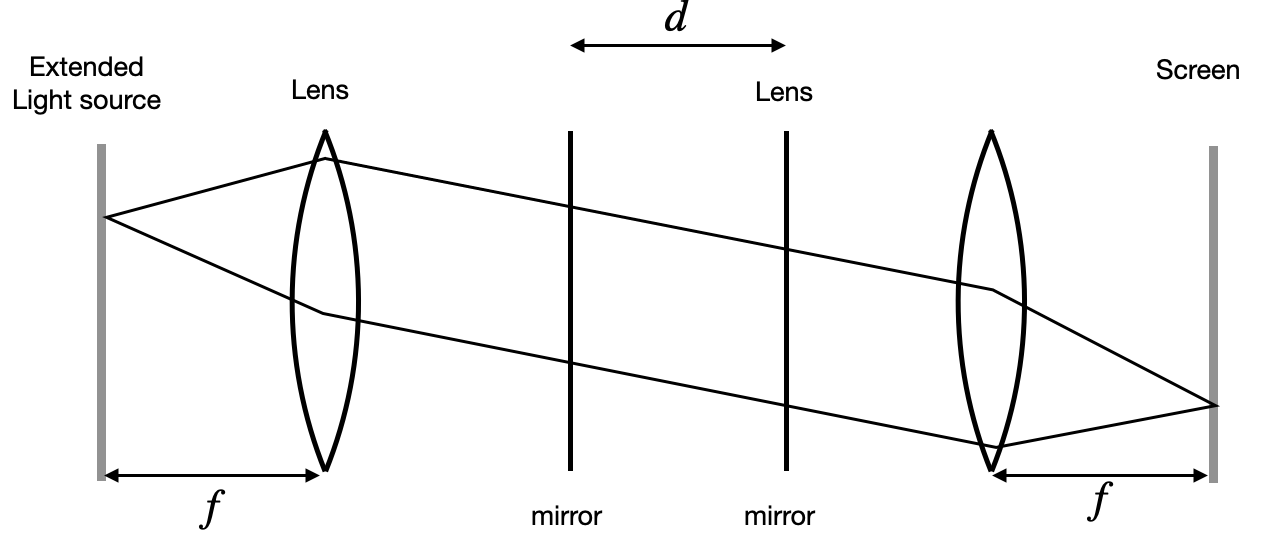
\includegraphics[width=0.9\linewidth,height=\textheight,keepaspectratio]{wave-optics/img/fabry_w_lens.png}

}

\caption{Fabry Perot Interferometer and interference pattern observed in
the lecture.}

\end{figure}%

The rings represent contours of constant phase difference, becoming more
closely spaced with increasing radius as demonstrated in these
experimental observations:

\begin{figure}

\begin{minipage}{0.50\linewidth}
\pandocbounded{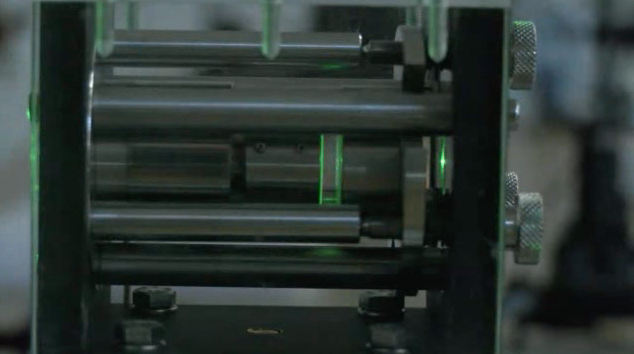
\includegraphics[keepaspectratio]{wave-optics/img/fabry_perot_lecture1.png}}\end{minipage}%
%
\begin{minipage}{0.50\linewidth}
\pandocbounded{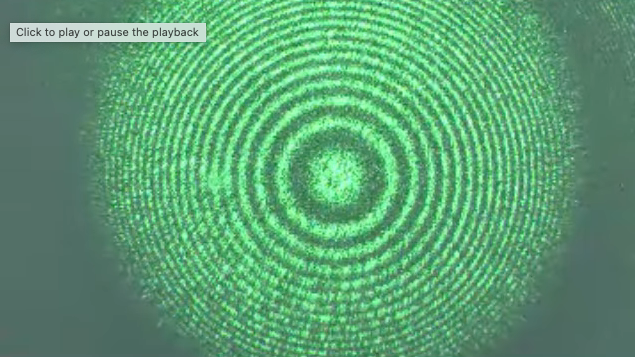
\includegraphics[keepaspectratio]{wave-optics/img/fabry_perot_lecture2.png}}\end{minipage}%

\caption{\label{fig-fabry}Fabry Perot Interferometer and interference
pattern observed in the lecture.}

\end{figure}%

This ring pattern is a powerful tool for spectroscopic analysis, as
different wavelengths produce distinct ring patterns, allowing precise
wavelength measurements and spectral analysis.

\begin{tcolorbox}[enhanced jigsaw, breakable, toptitle=1mm, bottomrule=.15mm, colbacktitle=quarto-callout-note-color!10!white, title=\textcolor{quarto-callout-note-color}{\faInfo}\hspace{0.5em}{Applications in Modern Research and Technology}, arc=.35mm, rightrule=.15mm, bottomtitle=1mm, opacityback=0, toprule=.15mm, coltitle=black, leftrule=.75mm, opacitybacktitle=0.6, colback=white, left=2mm, titlerule=0mm, colframe=quarto-callout-note-color-frame]

\textbf{Spectroscopy:}

\begin{itemize}
\tightlist
\item
  \textbf{High-Resolution Spectroscopy:} Fabry-Perot interferometers are
  used to achieve high spectral resolution, allowing precise
  measurements of spectral lines. This is crucial in fields like
  astrophysics, where detailed analysis of stellar spectra can reveal
  information about the composition, temperature, and motion of
  celestial objects.
\end{itemize}

\begin{figure}[H]

{\centering 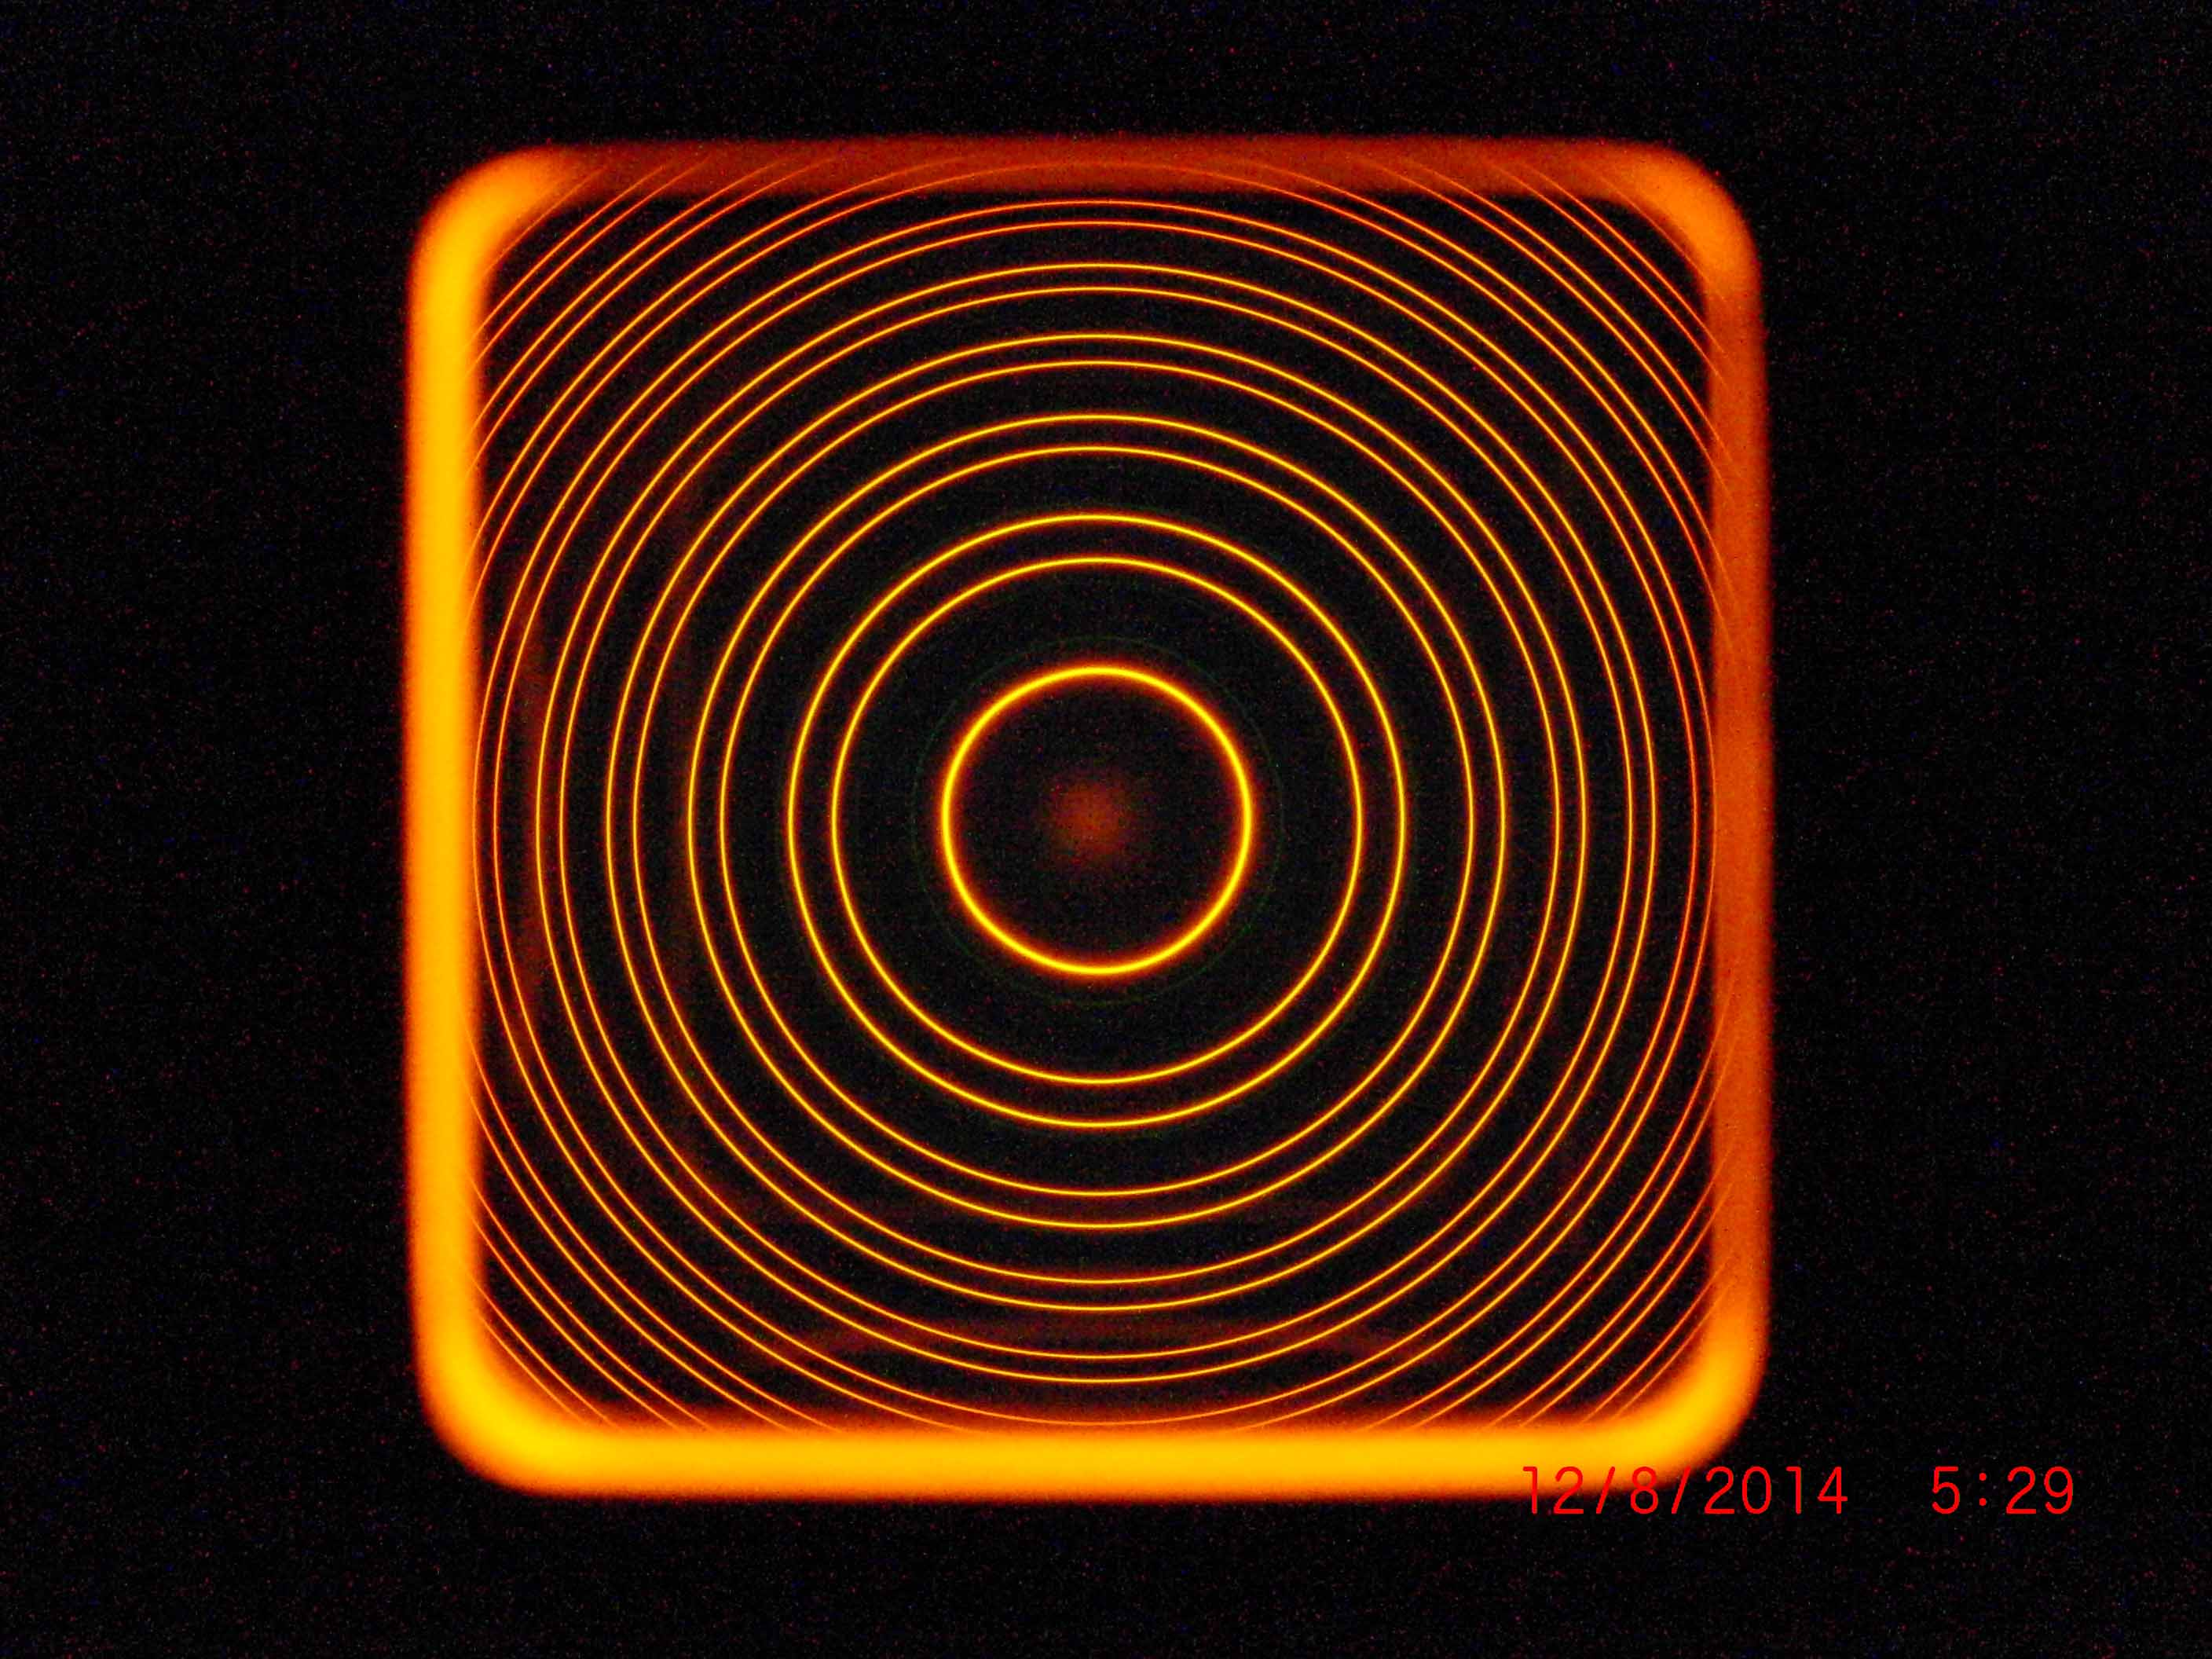
\includegraphics[width=0.5\linewidth,height=\textheight,keepaspectratio]{wave-optics/img/Sodium Rings Solid Etalon.jpg}

}

\caption{Sodium D Lines measured as 593.0 +/- 4.5 nm, 591.1 +/- 5.0 nm
with a difference of 0.604 +/- 0.025 (matching the accepted values of
589.5924 nm, 588.9951 with a difference of 0.5973 nm). Also courtesy of
Lake Forest College}

\end{figure}%

\begin{itemize}
\tightlist
\item
  \textbf{Laser Spectroscopy:} They are used to analyze the spectral
  properties of lasers, including linewidth, mode structure, and
  stability.
\end{itemize}

\textbf{Optical Communications:}

\begin{itemize}
\tightlist
\item
  \textbf{Wavelength Division Multiplexing (WDM):} Fabry-Perot filters
  are used in WDM systems to separate and combine different wavelength
  channels, increasing the data-carrying capacity of optical fibers.
\item
  \textbf{Laser Stabilization:} They help stabilize the wavelength of
  lasers used in optical communication systems, ensuring consistent
  performance and reducing signal degradation.
\end{itemize}

\textbf{Metrology:}

\begin{itemize}
\tightlist
\item
  \textbf{Precision Measurement:} Fabry-Perot interferometers are used
  for precise distance and displacement measurements. They can measure
  changes in length with sub-nanometer accuracy, making them valuable in
  applications like semiconductor manufacturing and materials science.
\item
  \textbf{Refractive Index Measurement:} They are used to measure the
  refractive index of gases, liquids, and solids with high precision.
\end{itemize}

\textbf{Laser Technology:}

\begin{itemize}
\tightlist
\item
  \textbf{Mode-Locking:} Fabry-Perot cavities are used in mode-locked
  lasers to produce ultra-short pulses of light, which are essential for
  applications in time-resolved spectroscopy, medical imaging, and
  telecommunications.
\item
  \textbf{Laser Tuning:} They are used to tune the wavelength of lasers,
  enabling precise control over the output wavelength for various
  applications.
\end{itemize}

\textbf{Environmental Monitoring:}

\begin{itemize}
\tightlist
\item
  \textbf{Gas Analysis:} Fabry-Perot interferometers are used in gas
  analyzers to detect and quantify trace gases in the atmosphere. This
  is important for monitoring air quality, greenhouse gas emissions, and
  industrial processes.
\item
  \textbf{Remote Sensing:} They are used in remote sensing instruments
  to analyze the spectral properties of reflected or emitted light from
  the Earth's surface and atmosphere, providing valuable data for
  climate studies and environmental monitoring.
\end{itemize}

\textbf{Astronomy:}

\begin{itemize}
\tightlist
\item
  \textbf{Interferometric Imaging:} Fabry-Perot interferometers are used
  in telescopes to enhance the resolution of astronomical images. They
  can be used to study fine details of celestial objects, such as the
  structure of galaxies and the dynamics of star-forming regions.
\item
  \textbf{Doppler Spectroscopy:} They are used to measure the Doppler
  shift of spectral lines, allowing astronomers to determine the radial
  velocity of stars and planets, which is crucial for the detection of
  exoplanets.
\end{itemize}

\textbf{Biomedical Applications:}

\begin{itemize}
\tightlist
\item
  \textbf{Optical Coherence Tomography (OCT):} Fabry-Perot
  interferometers are used in OCT systems to achieve high-resolution
  cross-sectional imaging of biological tissues. This is valuable for
  medical diagnostics, particularly in ophthalmology and dermatology.
  \pandocbounded{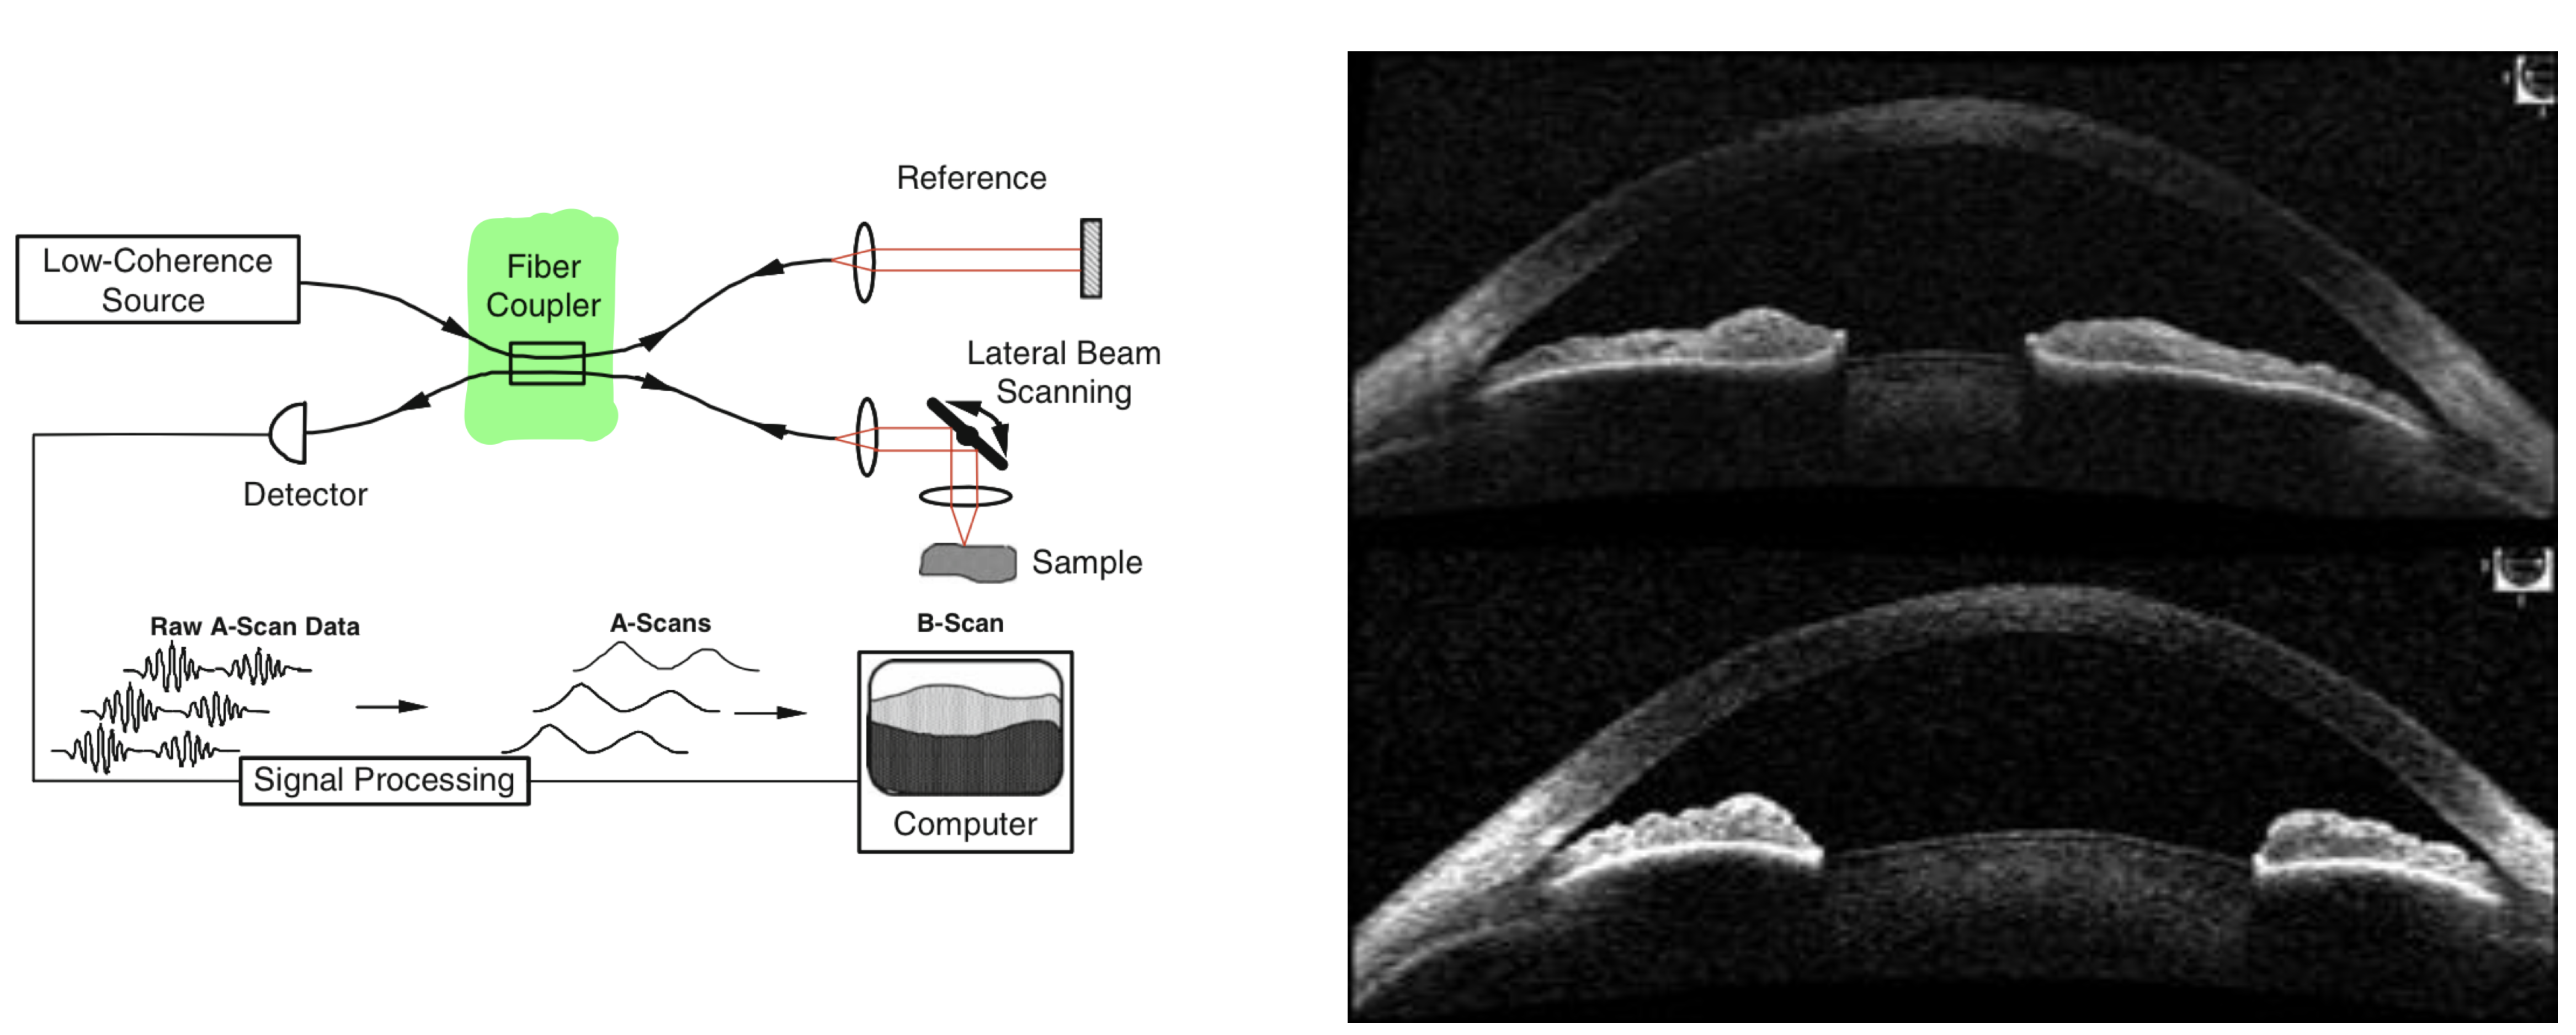
\includegraphics[keepaspectratio]{wave-optics/img/OCT.png}}
\item
  \textbf{Fluorescence Microscopy:} They are used to enhance the
  spectral resolution of fluorescence microscopes, enabling detailed
  analysis of biological samples.
\end{itemize}

\textbf{Quantum Optics:}

\begin{itemize}
\tightlist
\item
  \textbf{Cavity Quantum Electrodynamics (CQED):} Fabry-Perot cavities
  are used to study the interaction between light and matter at the
  quantum level. This research is fundamental for the development of
  quantum information technologies and quantum computing.
\item
  \textbf{Single-Photon Sources:} They are used to create and manipulate
  single-photon sources, which are essential for quantum communication
  and cryptography.
\end{itemize}

These applications highlight the versatility and importance of
Fabry-Perot interferometers in advancing scientific research and
technological innovation across various fields.

\end{tcolorbox}

\chapter{Diffraction}\label{diffraction}

\section{Huygens' Principle}\label{huygens-principle}

Formulated by Christiaan Huygens in 1678, \textbf{Huygens' principle}
states that every point on a wavefront acts as a source of secondary
spherical wavelets that spread out in the forward direction. The new
position of the wavefront at any later time is found by constructing a
surface tangent to these secondary wavelets. This principle provides a
powerful method for analyzing wave propagation and explains various wave
phenomena such as reflection, refraction, and diffraction.

\begin{figure}[H]

{\centering 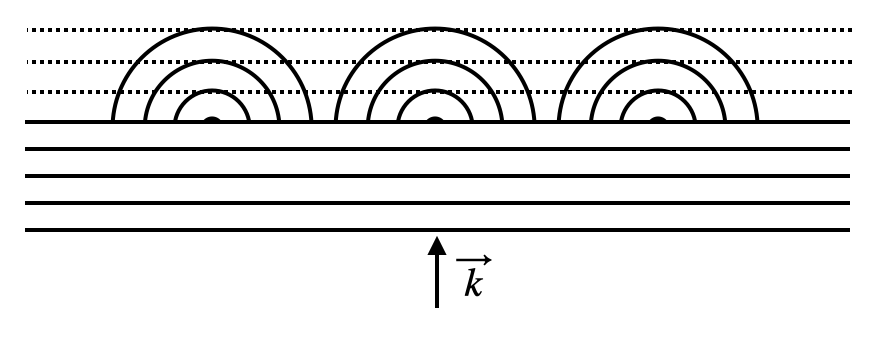
\includegraphics[width=0.4\linewidth,height=\textheight,keepaspectratio]{wave-optics/img/huygens.png}

}

\caption{Illustration of Huygens' principle for a plane wave incident
with a wave vector \(\vec{k}\). Each point on the wavefront acts as a
source of secondary wavelets, and the new wavefront is the envelope of
these wavelets.}

\end{figure}%

Huygens' principle can be demonstrated numerically and visually. By
placing a large number of spherical wave sources closely along a line
and allowing their waves to interfere, we can reconstruct a plane
wavefront propagating in the forward direction, illustrating how a plane
wave advances according to Huygens' concept.

\begin{figure}[H]

{\centering 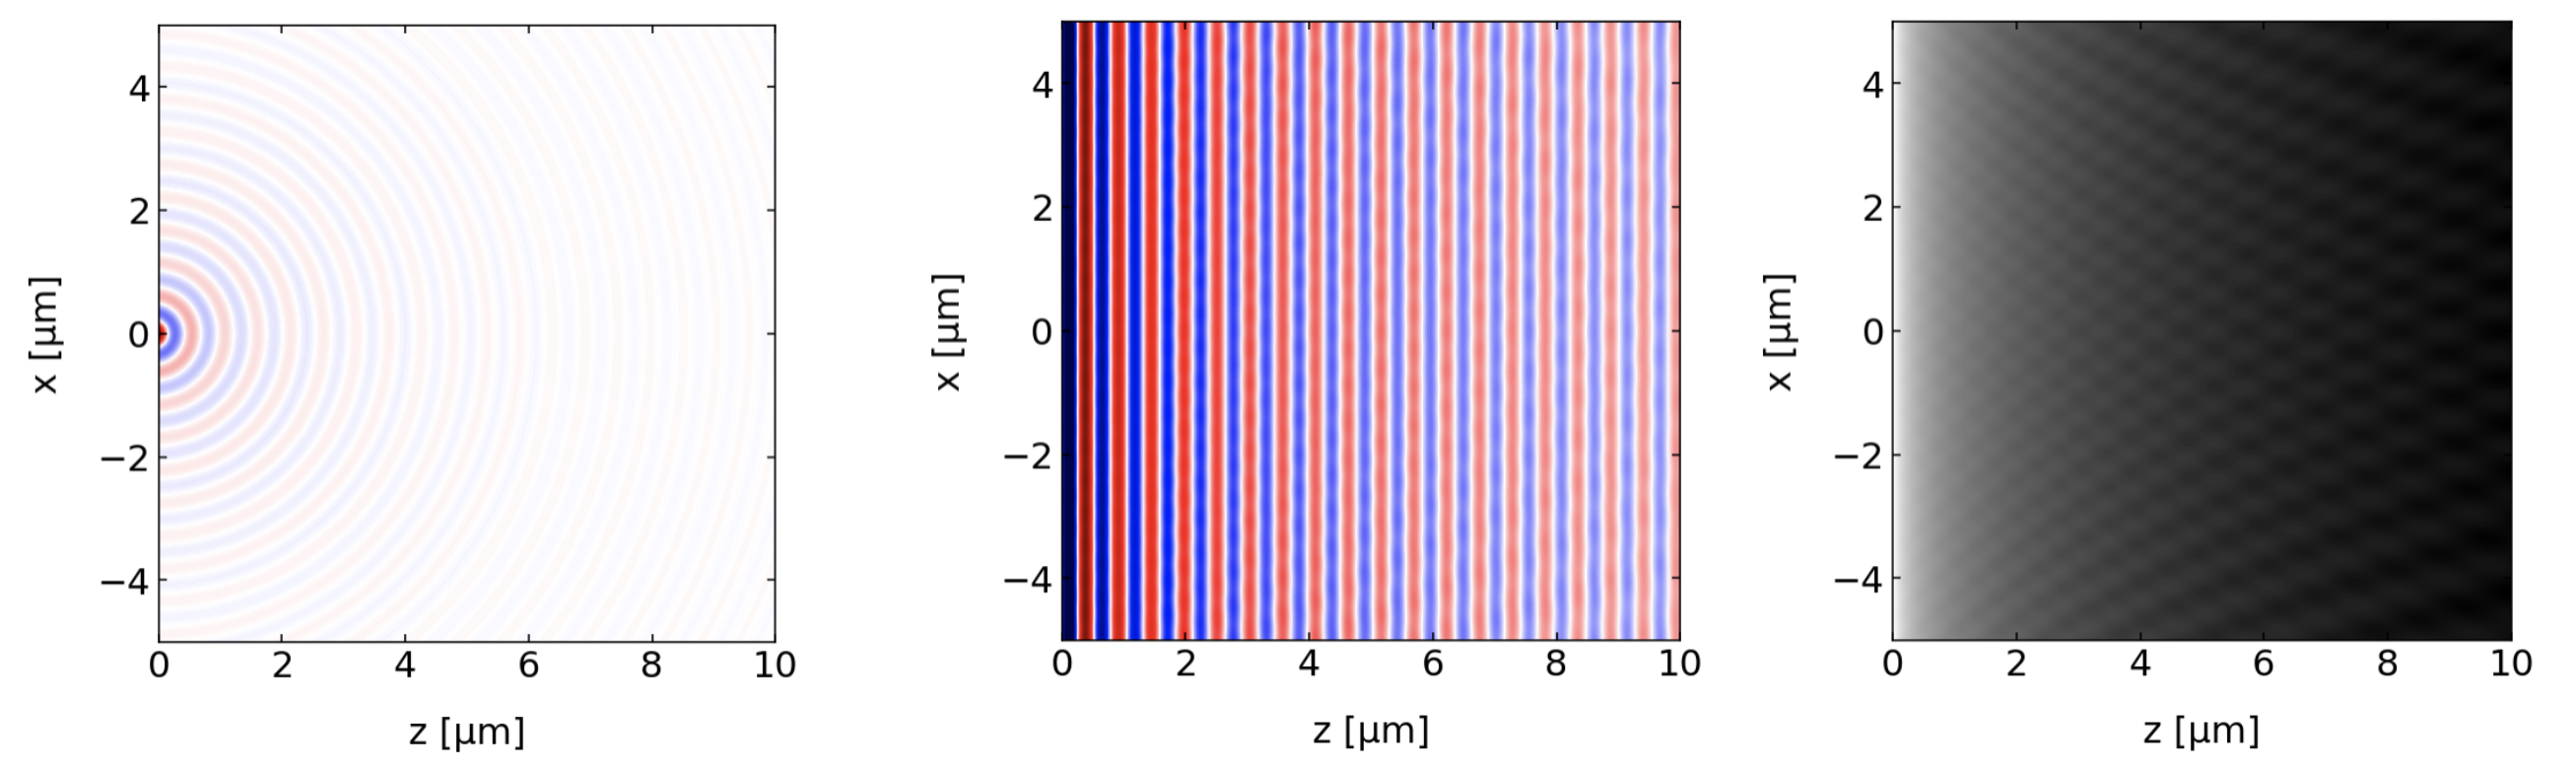
\includegraphics[width=1\linewidth,height=\textheight,keepaspectratio]{wave-optics/img/huygens_num.png}

}

\caption{Numerical demonstration of Huygens' principle used to recreate
a plane wave from a set of spherical waves. The graph on the left shows
the amplitude of a single spherical wave of wavelength \(\lambda=532\)
nm. By arranging 500 spherical wave sources densely along the x-axis at
\(z=0\), all in phase (representing the phase of the incident plane wave
at \(z=0\)), we can recreate the plane wavefronts for \(z>0\) (middle)
and the constant intensity distribution (right).}

\end{figure}%

Mathematically, this phenomenon can be described using our earlier
treatment of multi-wave interference. Consider \(M\) spherical wave
sources arranged along the x-axis at \(z=0\), each separated by a small
distance \(d\) from its neighbor. At a point far away from the sources
(in the far-field approximation), the path difference between waves from
adjacent sources leads to a phase difference given by:

\[
\Delta \phi = \frac{2\pi d \sin \theta }{\lambda}
\]

where \(\theta\) is the angle relative to the z-axis (the forward
direction), and \(\lambda\) is the wavelength of the waves. The
superposition of these waves results in an intensity pattern described
by:

\[
I(\theta) = I_0 \frac{\sin^2\left ( M \frac{\pi d \sin \theta }{\lambda} \right )}{\sin^2\left ( \frac{\pi d \sin \theta }{\lambda} \right )}
\]

This expression arises from the interference of \(M\) waves with a
constant phase difference \(\Delta \phi\) between neighboring waves. The
numerator represents the constructive and destructive interference due
to the finite number of sources, and the denominator accounts for the
spacing between them.

This mathematical framework serves as the foundation for understanding
diffraction phenomena, particularly in two important cases:

\begin{enumerate}
\def\labelenumi{\arabic{enumi}.}
\item
  \textbf{Single-Slit Diffraction}: When Huygens' wavelets are confined
  to a finite width (the slit width), the interference between these
  wavelets produces a characteristic diffraction pattern with a central
  maximum and diminishing side lobes.
\item
  \textbf{Diffraction Gratings}: When multiple slits are arranged
  periodically, the interference of the transmitted waves leads to sharp
  diffraction maxima at specific angles, making diffraction gratings
  powerful tools for spectroscopic analysis.
\end{enumerate}

While we commonly use the term ``diffraction'' to describe these
phenomena, they are fundamentally due to the interference of waves, as
explained by Huygens' principle. By considering every point on a
wavefront as a source of secondary wavelets, we can understand and
predict the complex patterns that arise when waves encounter obstacles
or apertures.

\section{Single Slit Diffraction}\label{single-slit-diffraction}

We now apply our interference formula to study the diffraction of an
incident plane wave (wavevector \(\vec{k}\)) on a single slit of width
\(b\). We can model this by placing a series of Huygens sources along
the slit opening. While the sketch below shows just 3 sources for
clarity, we'll generalize this to \(M\) sources.

\begin{center}
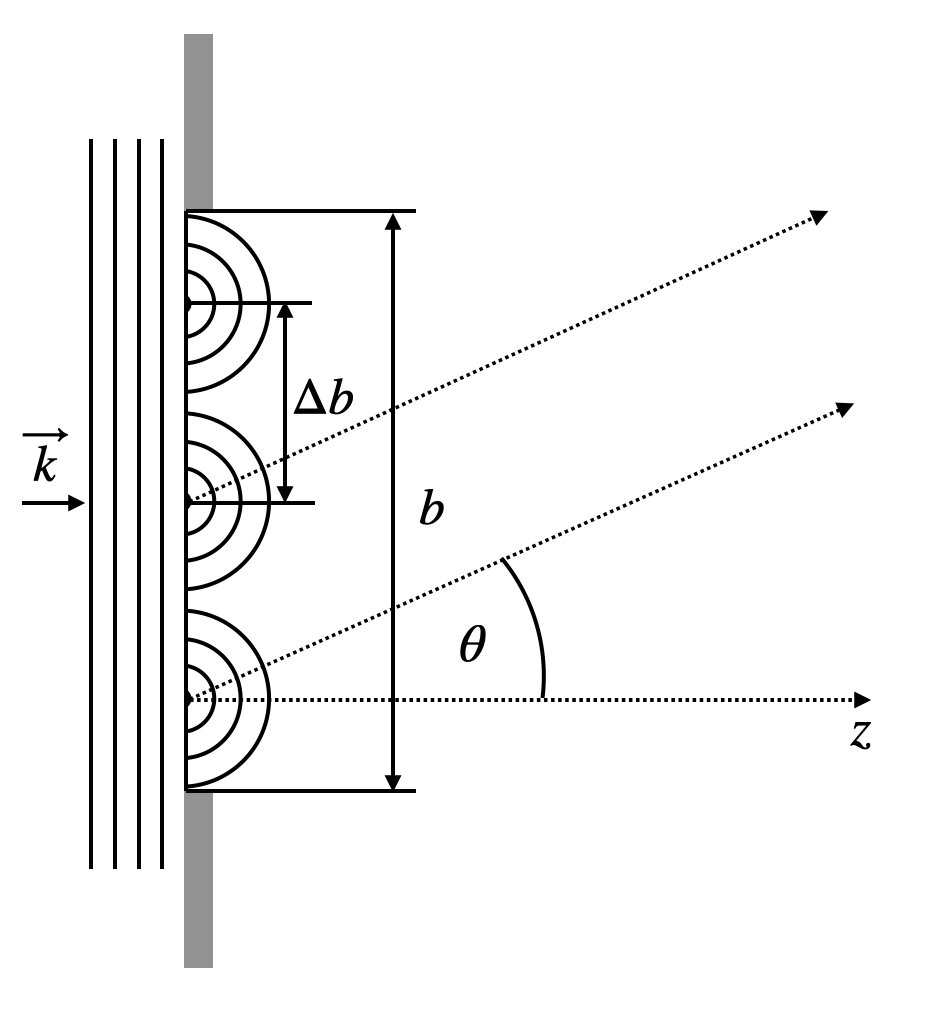
\includegraphics[width=4.16667in,height=\textheight,keepaspectratio]{wave-optics/img/single_slit.png}
\end{center}

We divide the slit into segments of width \(\Delta b\) such that we have
\(M=b/\Delta b\) Huygens sources, each with amplitude
\(A_0=\sqrt{I_0}\). Applying our previous multi-wave interference
formula with spacing \(d=\Delta b\), we obtain:

\[
I=I_0 \frac{\sin^2\left (M\pi\frac{\Delta b}{\lambda}\sin(\theta)\right)}{\sin^2\left (\pi\frac{\Delta b}{\lambda}\sin(\theta)\right)}
\]

Since \(M\Delta b = b\), we can rewrite this as:

\[
I=I_0 \frac{\sin^2\left (\pi\frac{b}{\lambda}\sin(\theta)\right)}{\sin^2\left (\pi\frac{b}{M\lambda}\sin(\theta)\right)}
\]

For convenience, let's substitute
\(x=\pi \frac{b}{\lambda}\sin(\theta)\), giving:

\[
I=I_0\frac{\sin^2(x)}{\sin^2(x/M)}
\]

In reality, we have a continuous distribution of sources across the slit
width, corresponding to \(M\to\infty\). In this limit, for the
denominator, \(x/M\) becomes very small, and we can use the small-angle
approximation:

\[
\sin^2\left (\frac{x}{M}\right) \approx \left(\frac{x}{M}\right)^2
\]

Therefore, our final expression becomes:

\[
I(\theta)=I_s\frac{\sin^2\left (\pi \frac{b}{\lambda}\sin(\theta)\right)}{\left(\pi \frac{b}{\lambda}\sin(\theta)\right)^2}
\]

where \(I_s=M^2I_0\) represents the total intensity from all sources.
This expression is often written using the sinc function (sinus
cardinalis):

\[
I(\theta)=I_s\,\text{sinc}^2\left(\pi \frac{b}{\lambda}\sin(\theta)\right)
\]

This formula describes the characteristic diffraction pattern of a
single slit, with a central maximum and symmetric side lobes of
decreasing intensity.

\begin{tcolorbox}[enhanced jigsaw, breakable, toptitle=1mm, bottomrule=.15mm, colbacktitle=quarto-callout-note-color!10!white, title=\textcolor{quarto-callout-note-color}{\faInfo}\hspace{0.5em}{Single Slit Diffraction}, arc=.35mm, rightrule=.15mm, bottomtitle=1mm, opacityback=0, toprule=.15mm, coltitle=black, leftrule=.75mm, opacitybacktitle=0.6, colback=white, left=2mm, titlerule=0mm, colframe=quarto-callout-note-color-frame]

The intensity distribution generated by the diffraction of monochromatic
light on a single slit and observed in the far field is given by

\[
I(\theta)=I_s\frac{\sin^2\left (\pi \frac{b}{\lambda}\sin(\theta)\right)}{\left( \pi \frac{b}{\lambda}\sin(\theta)\right)^2}
\]

where \(\lambda\) is the wavelength of the light and \(b\) the width of
the slit. The angle of observation is given by \(\theta\). Note that the
diffraction pattern on any aperture is resulting from the fact that you
remove Huygens sources that would be normally needed to form a plane
wavefront for example.

\textbf{Fourier Transform and Diffraction}

The intensity distribution generated by the diffraction of monochromatic
light on a single slit and observed in the far field is given by

\[
I(\theta)=I_s\frac{\sin^2\left (\pi \frac{b}{\lambda}\sin(\theta)\right)}{\left( \pi \frac{b}{\lambda}\sin(\theta)\right)^2}
\]

where \(\lambda\) is the wavelength of the light and \(b\) the width of
the slit. The angle of observation is given by \(\theta\). Note that the
diffraction pattern on any aperture is resulting from the fact that you
remove Huygens sources that would be normally needed to form a plane
wavefront for example.

This diffraction pattern can be understood as the Fourier transform of
the aperture function. In the case of a single slit, the aperture
function is a rectangular function, and its Fourier transform is a sinc
function. This relationship between the aperture and its diffraction
pattern is a fundamental concept in wave optics and is widely used in
various applications, including imaging and signal processing.

\end{tcolorbox}

\begin{figure}[H]

{\centering 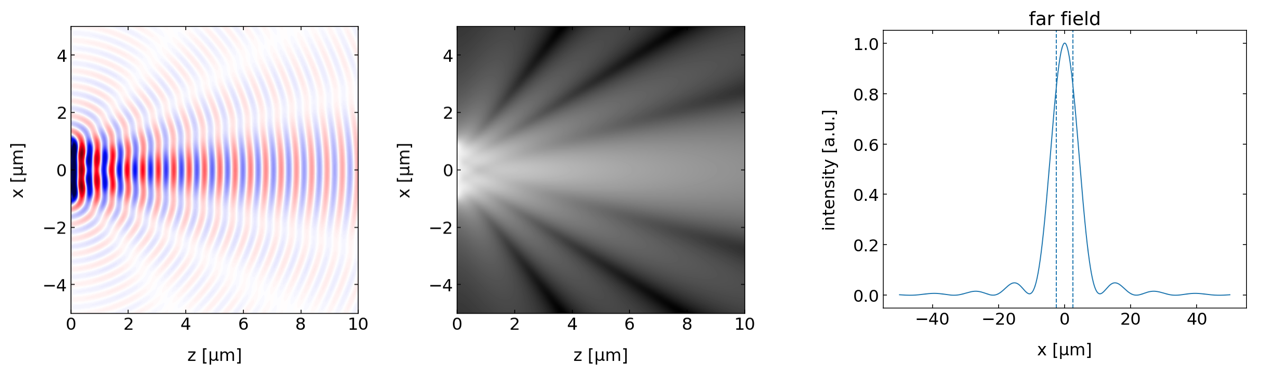
\includegraphics[width=1\linewidth,height=\textheight,keepaspectratio]{wave-optics/img/slit_intensity.png}

}

\caption{Total wave amplitude behind a slit (b=2µm) for an incident wave
of 532 nm wavelength. The plot in the middle shows the intensity in the
space behind the slit. The graph on the right displays the diffraction
pattern at a screen at 100 µm distance from the slit.}

\end{figure}%

Let's have a look at some of the properties of the intensity
distribution.

\begin{figure}[H]

{\centering \pandocbounded{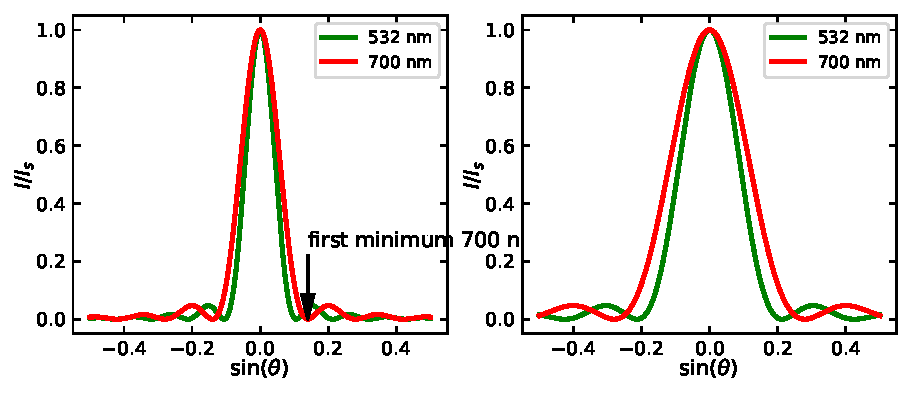
\includegraphics[keepaspectratio]{wave-optics/Diffraction_files/figure-pdf/cell-3-output-1.pdf}}

}

\caption{Caption}

\end{figure}%

The single-slit diffraction pattern shows characteristic features that
we can observe in both theoretical calculations and experimental
measurements. The intensity distribution is described by an oscillating
function with decreasing amplitude. The oscillations arise from the
\(\sin^2\) term in the numerator, while the decay comes from the square
term in the denominator.

\begin{figure}[H]

{\centering 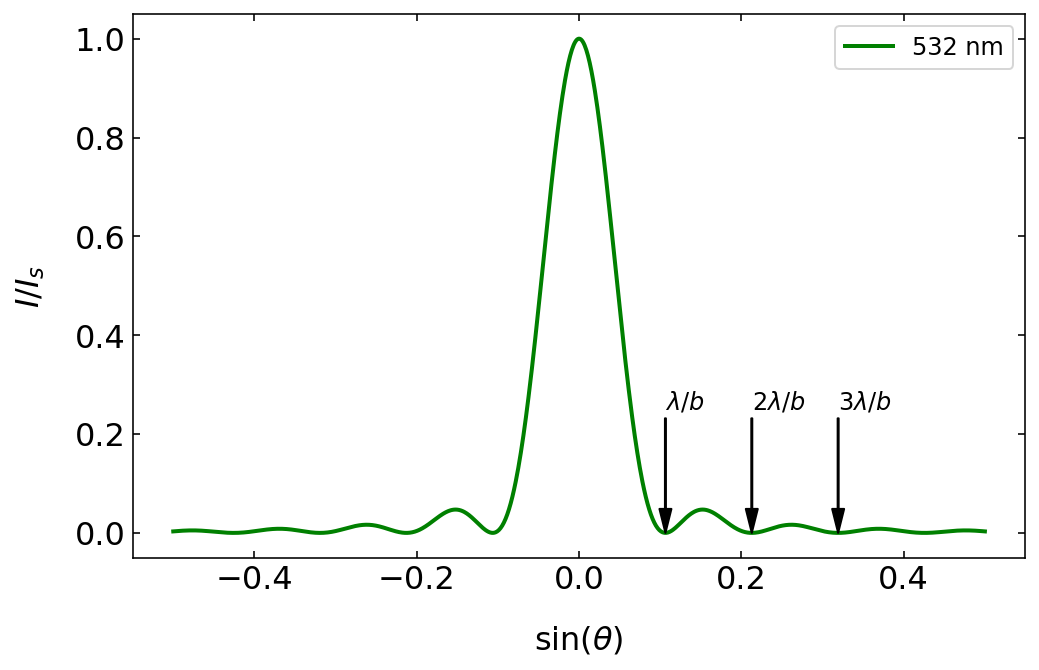
\includegraphics[width=4.16667in,height=\textheight,keepaspectratio]{wave-optics/img/slit_diff_min.png}

}

\caption{Diffraction patterns as a function of the sine of the
diffraction angle. The minima of the diffraction pattern in this plot
are at integer multiples of \(\lambda/b\).}

\end{figure}%

The graphs above illustrate two key relationships in single-slit
diffraction:

\begin{enumerate}
\def\labelenumi{\arabic{enumi}.}
\tightlist
\item
  The effect of wavelength: When comparing patterns for different
  wavelengths (with fixed slit width \(b=5\,\mathrm{\mu m}\)), longer
  wavelengths produce broader diffraction patterns
\item
  The effect of slit width: For the same wavelength, reducing the slit
  width to \(b=2.5\,\mathrm{\mu m}\) results in a broader diffraction
  pattern
\end{enumerate}

These observations can be quantified by analyzing the positions of
intensity minima. The intensity goes to zero when the argument of the
sine function in the numerator equals multiples of π:

\[
\pi \frac{b}{\lambda}\sin(\theta) = m\pi
\]

where \(m\) is an integer. This simplifies to:

\[
\sin(\theta)=m\frac{\lambda}{b}
\]

This relationship reveals a fundamental principle in diffraction: the
angular spread of the pattern is proportional to the ratio of wavelength
to the size of the diffracting object (\(\lambda/b\)). While the exact
mathematical form may vary for different geometries, this basic scaling
remains valid.

\begin{figure}

\begin{minipage}{0.50\linewidth}
\pandocbounded{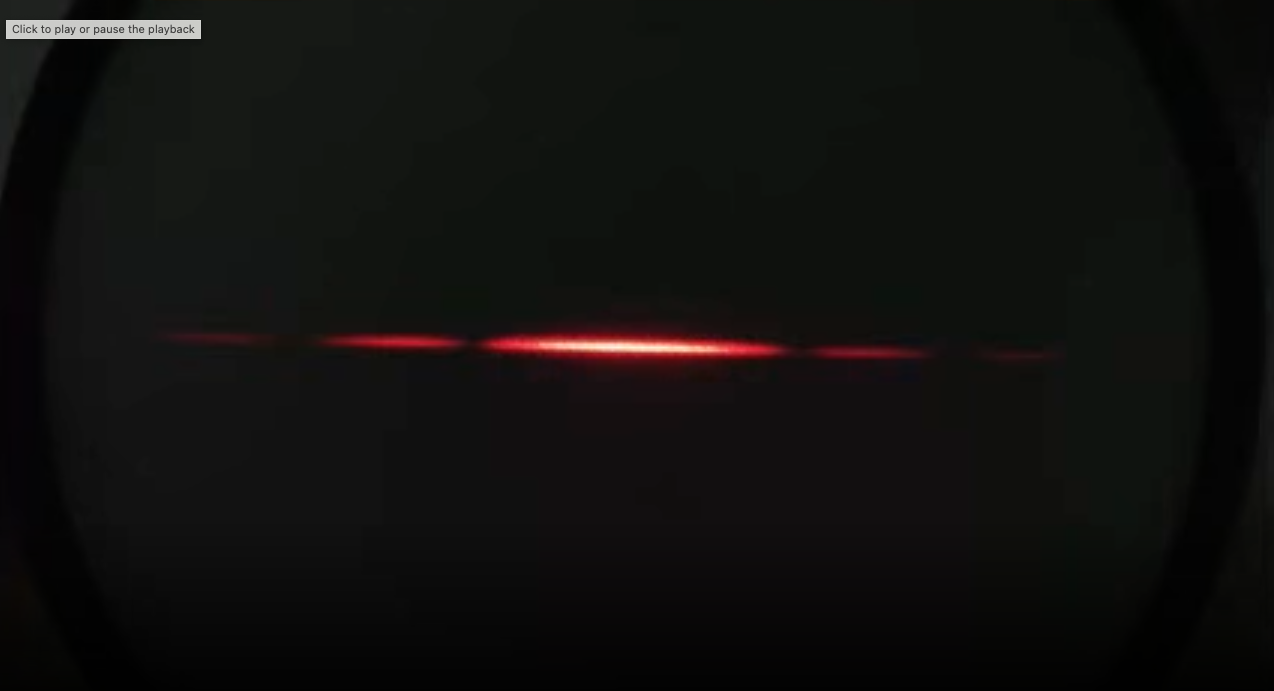
\includegraphics[keepaspectratio]{wave-optics/img/single_slit1.png}}\end{minipage}%
%
\begin{minipage}{0.50\linewidth}
\pandocbounded{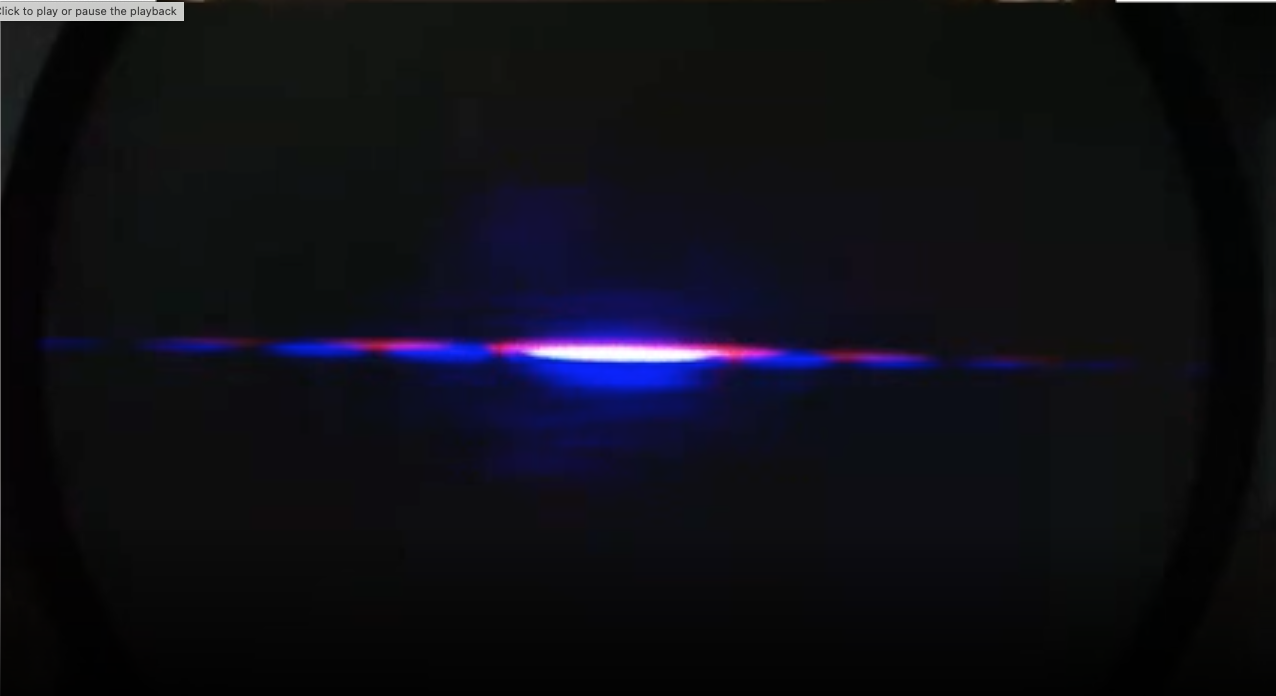
\includegraphics[keepaspectratio]{wave-optics/img/single_slit2.png}}\end{minipage}%

\caption{\label{fig-slitdiff}Diffraction patterns on a single slit as
observed in the lecture. The left image shows the diffraction pattern
for red light, while the right image combines two different wavelengths
(red, blue), where one clearly recognizes the wider diffraction peaks
for the longer red wavelength.}

\end{figure}%

The experimental observations above clearly demonstrate these
principles, particularly showing how red light (longer wavelength)
produces a broader diffraction pattern than blue light (shorter
wavelength).

\section{Circular Aperture}\label{circular-aperture}

For a circular aperture, the diffraction pattern follows a more complex
mathematical form involving Bessel functions. The intensity distribution
is given by:

\[
I(\theta)=I_0\left( \frac{2J_1(x)}{x} \right )^2
\]

where \(J_1\) is the
\href{https://en.wikipedia.org/wiki/Bessel_function}{Bessel function} of
the first kind, and

\[
x=\frac{2\pi R}{\lambda}\sin(\theta)
\]

Here, \(R\) is the radius of the aperture. While similar to the sine
function, the Bessel function has zeros at different positions:
\(x_1=1.22\pi\), \(x_2=2.23\pi\), and so on.

\begin{figure}[H]

{\centering 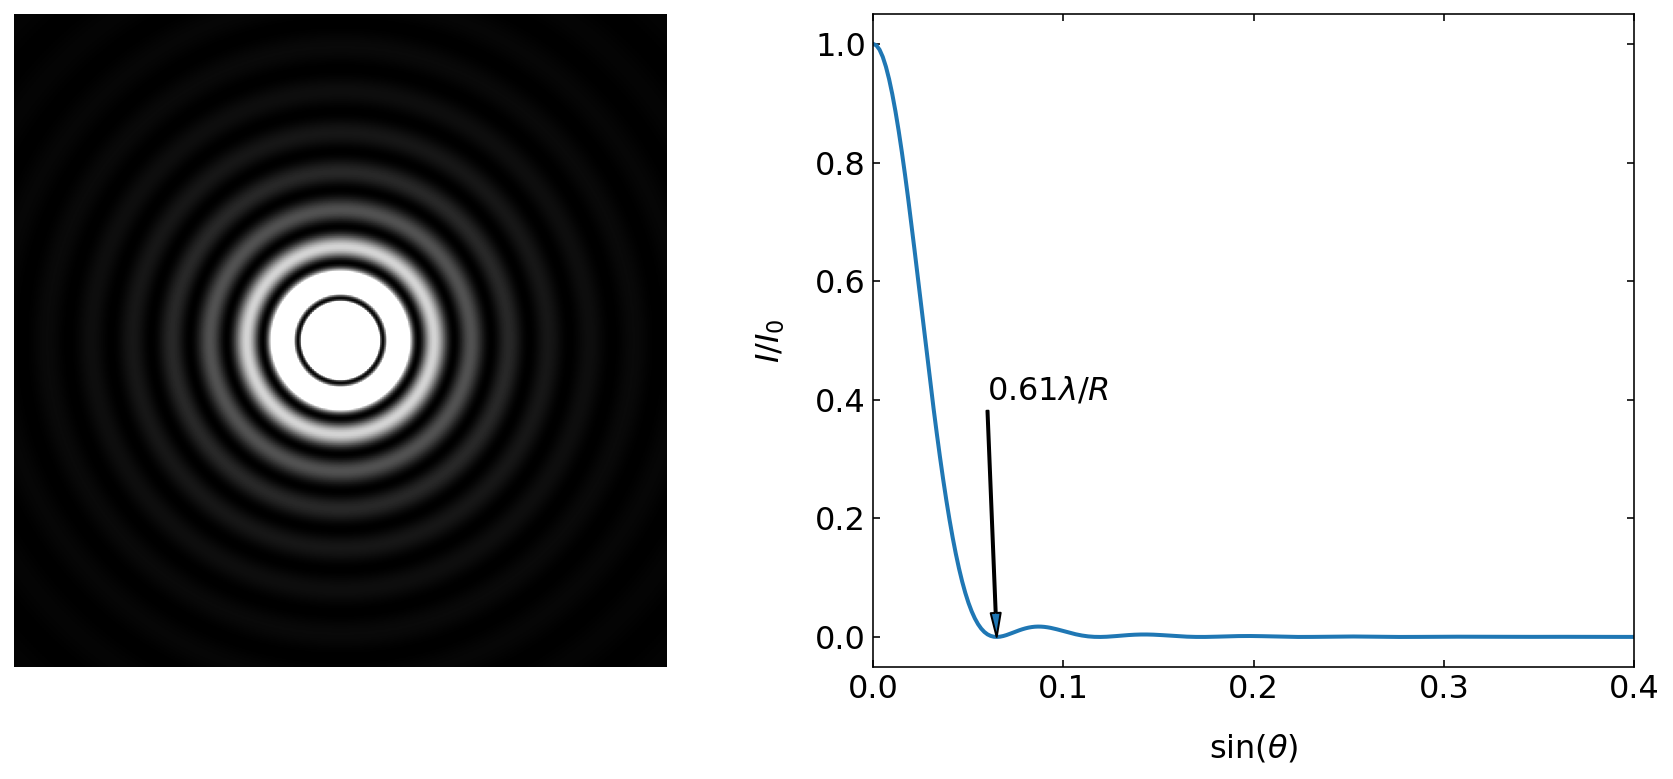
\includegraphics[width=0.9\linewidth,height=\textheight,keepaspectratio]{wave-optics/img/circ_ap.png}

}

\caption{Diffraction pattern of a circular aperture of radius \(5\) µm.
Note that the intensity scale is saturated. The diffraction rings would
otherwise not be visible. The minima of the diffraction pattern in this
plot are at integer multiples of \(0.61\lambda/R\).}

\end{figure}%

The first minimum of the diffraction pattern occurs when:

\[
x_1=1.22\pi=\frac{2\pi R}{\lambda}\sin(\theta_1)
\]

Solving for \(\sin(\theta_1)\):

\[
\sin(\theta_1)=0.61\frac{\lambda}{R}
\]

This follows the same general principle we've seen before: the angular
spread is proportional to wavelength divided by aperture size. The
central bright region up to this first minimum is known as the
\textbf{Airy disc}, and in microscopy, this defines a resolution element
or \textbf{resel}.

\begin{center}\rule{0.5\linewidth}{0.5pt}\end{center}

\section{Application: Diffraction
Grating}\label{application-diffraction-grating}

We now combine the concepts of single-slit diffraction and multiple-wave
interference to understand the behavior of diffraction gratings.
Diffraction gratings are important in spectroscopy and the compression
of short laser pulses.

Consider a diffraction grating with \(N\) slits, each of width \(b\),
and separated by a distance \(d\). Each slit acts as a source of
diffraction, producing an intensity pattern that oscillates with
decreasing amplitude. The width of this diffraction pattern is
determined by \(\lambda/b\), and the pattern is given by:

\[
I(\theta) = I_s \frac{\sin^2\left(\pi \frac{b}{\lambda} \sin(\theta)\right)}{\left(\pi \frac{b}{\lambda} \sin(\theta)\right)^2}
\]

Now, we have multiple slits, each separated by a distance \(d\). The
interference of waves from these slits is described by:

\[
I = I_0 \frac{\sin^2(N \phi / 2)}{\sin^2(\phi / 2)}
\]

where the phase difference \(\phi\) between waves from neighboring slits
is given by:

\[
\phi = k \Delta s = \frac{2\pi}{\lambda} d \sin(\theta)
\]

Combining these expressions, the intensity distribution for a
diffraction grating is:

\[
I(\theta) = I_0 \frac{\sin^2\left(\pi \frac{b}{\lambda} \sin(\theta)\right)}{\left(\pi \frac{b}{\lambda} \sin(\theta)\right)^2} \frac{\sin^2\left(N \pi \frac{d}{\lambda} \sin(\theta)\right)}{\sin^2\left(\pi \frac{d}{\lambda} \sin(\theta)\right)}
\]

This formula describes the intensity pattern produced by a diffraction
grating, which is the product of the single-slit diffraction pattern and
the multiple-slit interference pattern.

\begin{tcolorbox}[enhanced jigsaw, breakable, toptitle=1mm, bottomrule=.15mm, colbacktitle=quarto-callout-note-color!10!white, title=\textcolor{quarto-callout-note-color}{\faInfo}\hspace{0.5em}{Diffraction Grating}, arc=.35mm, rightrule=.15mm, bottomtitle=1mm, opacityback=0, toprule=.15mm, coltitle=black, leftrule=.75mm, opacitybacktitle=0.6, colback=white, left=2mm, titlerule=0mm, colframe=quarto-callout-note-color-frame]

The intensity distribution generated by a diffraction grating from
monochromatic light and observed in the far field is given by

\[
I(\theta) = I_0 \frac{\sin^2\left(\pi \frac{b}{\lambda} \sin(\theta)\right)}{\left(\pi \frac{b}{\lambda} \sin(\theta)\right)^2} \frac{\sin^2\left(N \pi \frac{d}{\lambda} \sin(\theta)\right)}{\sin^2\left(\pi \frac{d}{\lambda} \sin(\theta)\right)}
\]

where \(\lambda\) is the wavelength of the light, \(b\) is the width of
the slit, \(d\) is the distance between the slits, and \(N\) is the
number of slits illuminated. The angle of observation is given by
\(\theta\).

\end{tcolorbox}

\subsection{Properties of the Diffraction
Pattern}\label{properties-of-the-diffraction-pattern}

Let's examine the properties of this intensity distribution. The graph
below shows the intensity distribution for a diffraction grating with
\(N=8\) slits, a slit distance of \(d=4\) µm, a slit width of \(b=2\)
µm, and a wavelength of 532 nm. We observe the following general
properties:

\begin{itemize}
\tightlist
\item
  The intensity pattern consists of main maxima, called
  \textbf{diffraction orders}, characterized by integer numbers. The
  central peak is the 0th order peak, the first main peak to the right
  is the 1st diffraction order, and so on.
\item
  The main peaks are separated by \(N-2\) secondary peaks and \(N-1\)
  minima.
\item
  The intensity distribution is characterized by an envelope, which is
  the diffraction pattern of a single slit (dashed line). In the example
  below, the 2nd order peak is suppressed. The envelope becomes wider if
  the slits become narrower.
\end{itemize}

\subsection{Position of the Main
Peaks}\label{position-of-the-main-peaks}

The position of the main peaks is determined by the condition that the
denominator of the multiple-slit interference term is zero. This occurs
when the argument is an integer multiple of \(\pi\), i.e.,
\(\pi \frac{d}{\lambda} \sin(\theta) = m\pi\), or:

\[
\sin(\theta) = m \frac{\lambda}{d}
\]

where \(m\) is an integer. The first-order diffraction maximum is found
at \(\sin(\theta) = \frac{\lambda}{d}\), independent of the number of
slits \(N\). This means that the position of the main peaks increases
linearly with the wavelength \(\lambda\) and decreases with increasing
slit distance \(d\).

\begin{figure}[H]

{\centering \pandocbounded{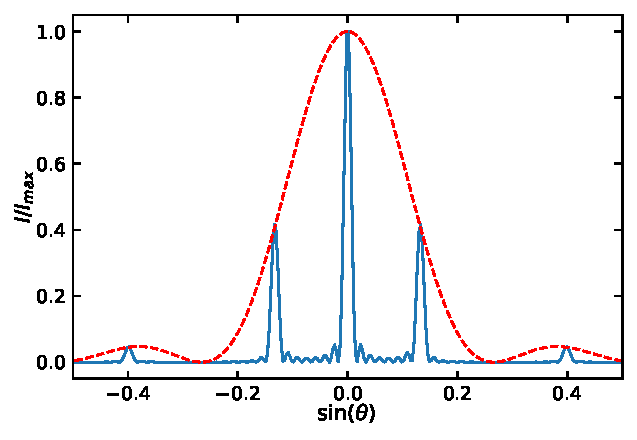
\includegraphics[keepaspectratio]{wave-optics/Diffraction_files/figure-pdf/cell-4-output-1.pdf}}

}

\caption{Diffraction pattern of a grating where 8 slits with a width of
2 µm and a distance of 4 micrometers are illuminated by a wavelength of
532 nm.}

\end{figure}%

\subsection{Influence of the Slit
Width}\label{influence-of-the-slit-width}

The two plots below show the influence of the slit width while keeping
the slit distance the same. We have \(N=8\) slits with \(d=4\) µm, while
the slit width is \(b=2\) µm on the left side and \(b=1\) µm on the
right side. The result is an increased width of the envelope. The first
minimum of the slit diffraction pattern occurs at
\(\sin(\theta) = \frac{\lambda}{b}\).

\begin{figure}[H]

{\centering \pandocbounded{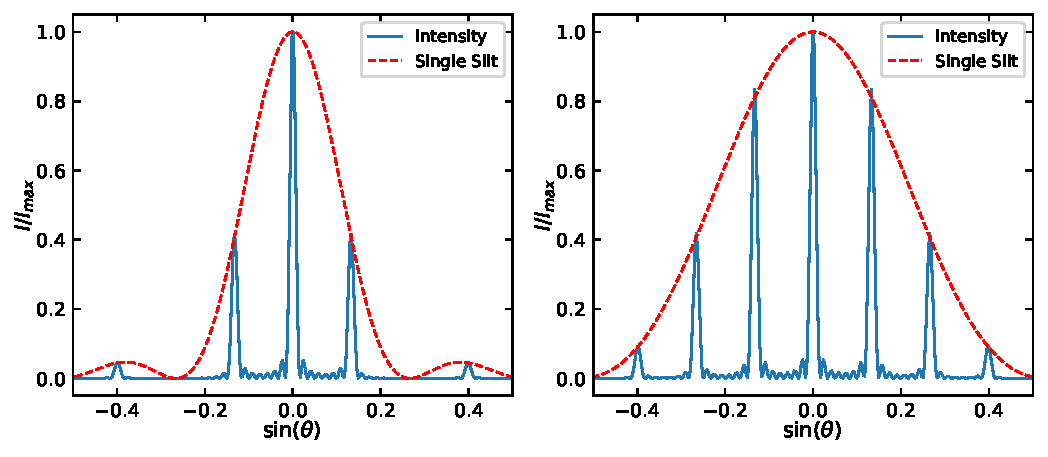
\includegraphics[keepaspectratio]{wave-optics/Diffraction_files/figure-pdf/cell-5-output-1.pdf}}

}

\caption{Diffraction pattern of a grating with \(N=8\) slits (\(d=4\)
µm, \(b=1\) µm) with \(\lambda=532\) nm.}

\end{figure}%

\subsection{Influence of the Slit
Number}\label{influence-of-the-slit-number}

When increasing the number of slits, the main diffraction peaks become
sharper. The location of the main peaks for a given wavelength remains
unchanged, but there are now \(N-2\) secondary maxima in between. This
decreased width of the main peaks is important for the spectral
resolution of the grating.

\begin{figure}[H]

{\centering \pandocbounded{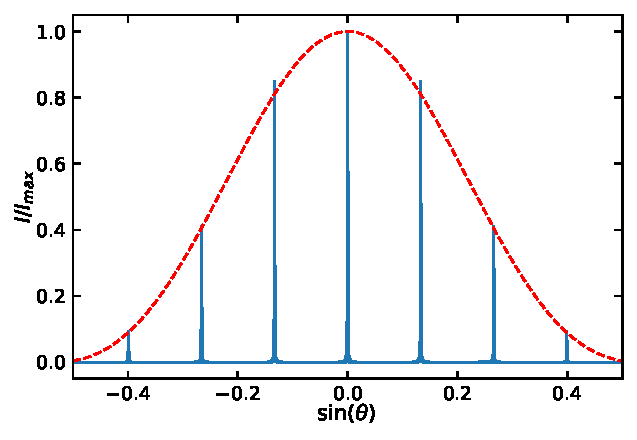
\includegraphics[keepaspectratio]{wave-optics/Diffraction_files/figure-pdf/cell-6-output-1.pdf}}

}

\caption{Diffraction pattern of a grating with \(N=100\) slits (\(d=4\)
µm, \(b=1\) µm) with \(\lambda=532\) nm.}

\end{figure}%

\subsection{Spectral Resolution}\label{spectral-resolution-1}

To quantify the spectral resolution, we use a criterion similar to the
optical resolution of a microscope: two peaks are separable if the
second peak is located at the minimum of the first diffraction pattern.
Here, the diffraction patterns refer to different wavelengths
\(\lambda_1\) and \(\lambda_2\).

\begin{figure}[H]

{\centering \pandocbounded{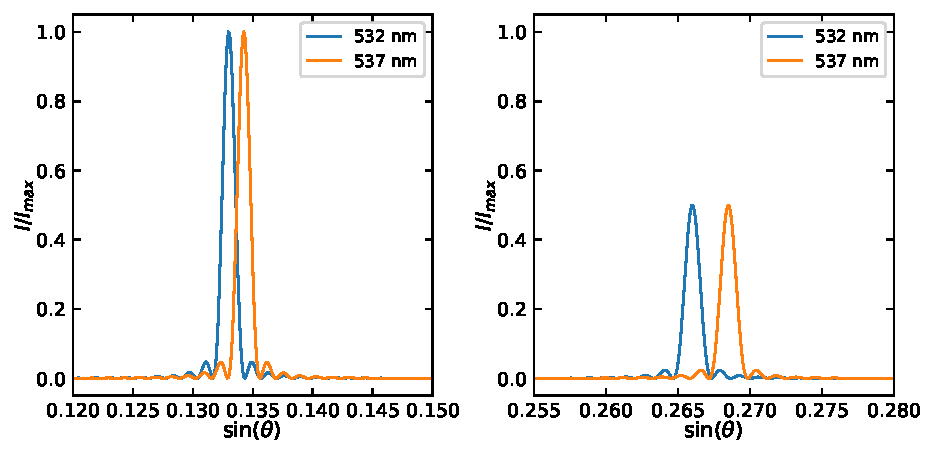
\includegraphics[keepaspectratio]{wave-optics/Diffraction_files/figure-pdf/cell-7-output-1.pdf}}

}

\caption{Rayleigh resolution limit of a grating with \(N=100\) slits
(\(d=4\) µm, \(b=1\) µm) with \(\lambda_1=532\) nm and \(\lambda_2=537\)
nm in the first order diffraction peak (left) and the second order peak
(right).}

\end{figure}%

Consider the \(m\)th order diffraction peak for the wavelength
\(\lambda_1\). This occurs at:

\[
\sin(\theta) = m \frac{\lambda_1}{d}
\]

The next secondary minimum to larger angles of the diffraction pattern
is located where the numerator of the multiple-wave interference term:

\[
\sin^2\left(N \pi \frac{d}{\lambda} \sin(\theta)\right)
\]

becomes zero, or the argument:

\[
N \pi \frac{d}{\lambda} \sin(\theta) = l \pi
\]

becomes a multiple \(l\) of \(\pi\). For the first-order main peak, we
have \(N-2\) intermediate peaks as well as the 0th and now the
first-order peak. Therefore, \(m = l/N\), and the next minimum after the
1st order peak is at:

\[
\sin(\theta_1) = \frac{l+1}{N} \frac{\lambda_1}{d}
\]

This angle must correspond to the position of the main peak of the
first-order diffraction of the wavelength \(\lambda_2\), so:

\[
\sin(\theta_1) = m \frac{\lambda_2}{d}
\]

Combining both equations for the two wavelengths yields:

\[
\left(m + \frac{1}{N}\right) \frac{\lambda_1}{d} = m \frac{\lambda_2}{d}
\]

and after some rearrangements (setting \(\lambda_1 = \lambda\)):

\[
R = \frac{\lambda}{\Delta \lambda} = mN
\]

This is the resolving power \(R\) of a grating. The ability to resolve
two wavelengths increases with the diffraction order \(m\) and the
number of slits used for the diffraction. However, the intensity of
higher diffraction orders rapidly decreases due to the grating envelope.
Therefore, the main parameter to change is the number of illuminated
slits.

Our finding is illustrated in the figure above, where we achieve a
resolution of about 5 nm when using \(N=100\) slits at a distance of
\(d=4\) µm.

\begin{figure}

\begin{minipage}{0.50\linewidth}

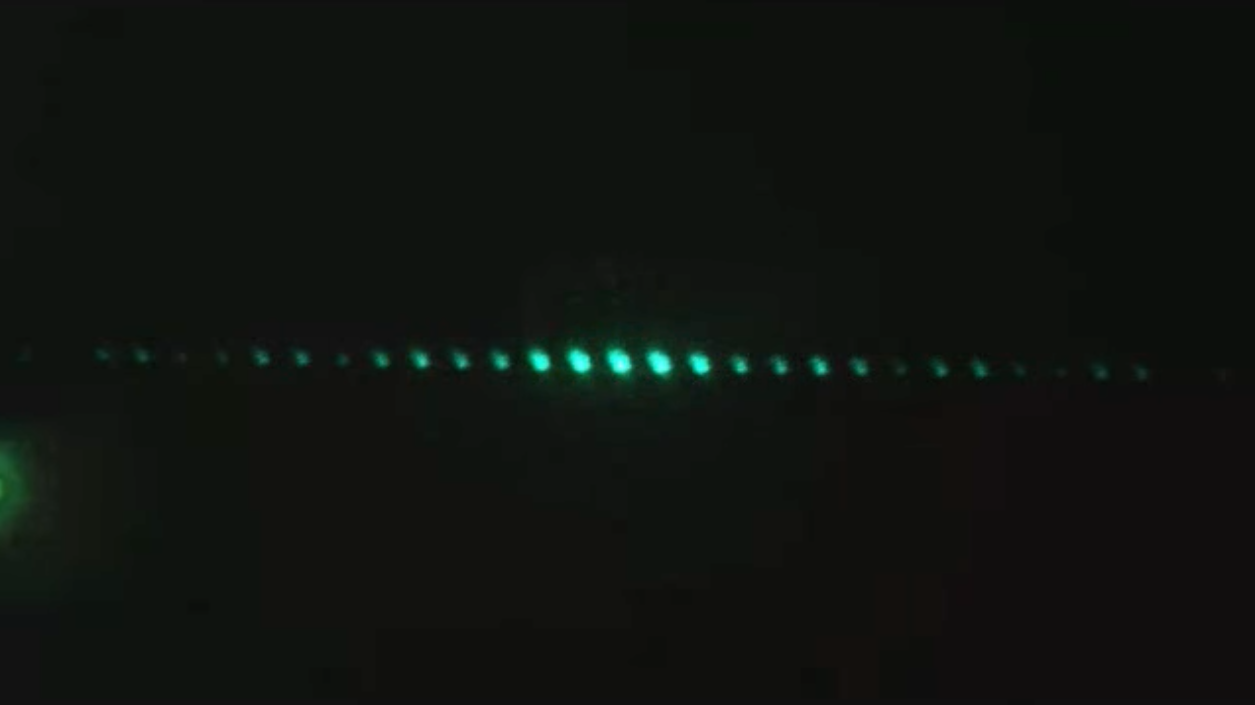
\includegraphics[width=0.8\linewidth,height=\textheight,keepaspectratio]{wave-optics/img/red_light_grating.png}

\subcaption{\label{}Diffraction pattern observed for a grating in the
lecture with red light (left) and white light (right).}
\end{minipage}%
%
\begin{minipage}{0.50\linewidth}

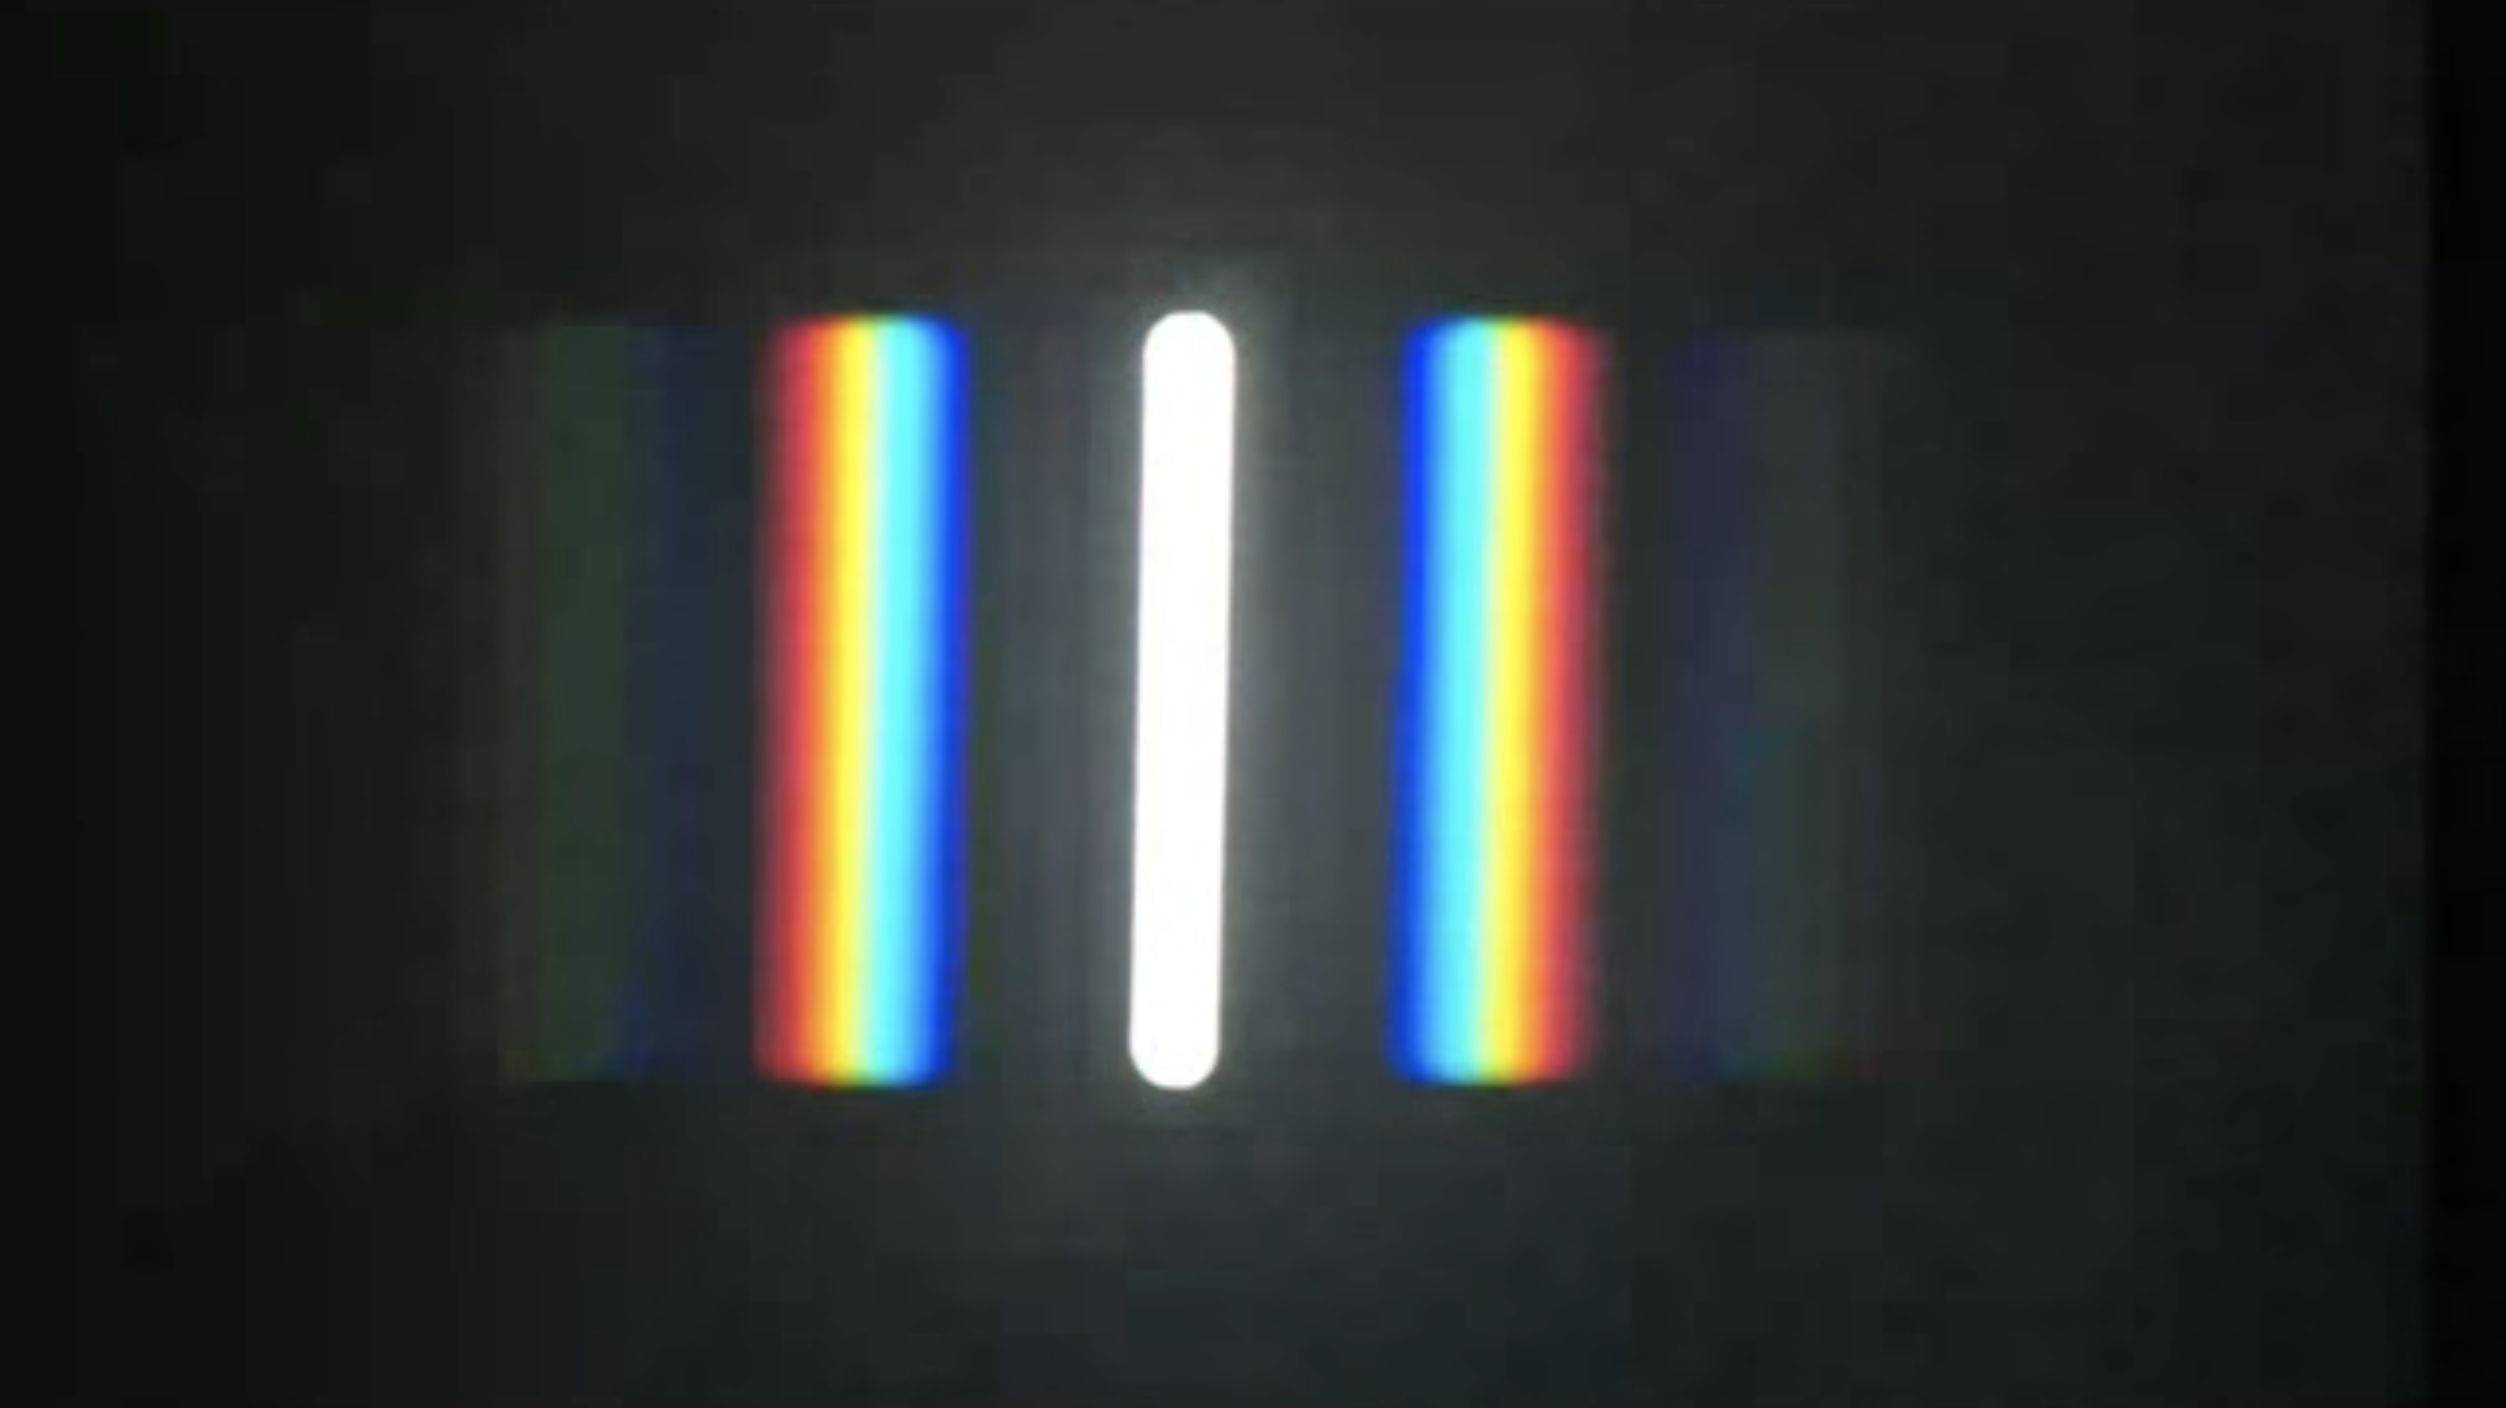
\includegraphics[width=0.8\linewidth,height=\textheight,keepaspectratio]{wave-optics/img/white_light_grating.png}

\subcaption{\label{}Diffraction pattern observed for a grating in the
lecture with red light (left) and white light (right).}
\end{minipage}%

\caption{\label{fig-grating}Diffraction pattern observed for a grating
in the lecture with red light (left) and white light (right).}

\end{figure}%

\begin{tcolorbox}[enhanced jigsaw, breakable, toptitle=1mm, bottomrule=.15mm, colbacktitle=quarto-callout-note-color!10!white, title=\textcolor{quarto-callout-note-color}{\faInfo}\hspace{0.5em}{Diffraction Grating Playground}, arc=.35mm, rightrule=.15mm, bottomtitle=1mm, opacityback=0, toprule=.15mm, coltitle=black, leftrule=.75mm, opacitybacktitle=0.6, colback=white, left=2mm, titlerule=0mm, colframe=quarto-callout-note-color-frame]

App to play with the parameters of a grating with a slit distance of 4
µm and a slit width of 2 µm.

\end{tcolorbox}

\chapter{Diffraction in Applications}\label{diffraction-in-applications}

\section{Application: Diffraction in the Human
Eye}\label{application-diffraction-in-the-human-eye}

The human eye provides an excellent real-world example of circular
aperture diffraction through the pupil (the opening in the iris). By
examining how light diffracts as it enters the eye, we can understand
fundamental limits on visual resolution and how the eye is naturally
optimized to these constraints.

\textbf{Calculating the Diffraction Limit of the Eye}

When light passes through the circular aperture of the pupil, it
undergoes diffraction, producing an Airy disk pattern on the retina. The
angle to the first minimum (dark ring) of the diffraction pattern is
given by:

\[
\sin(\theta_1) = 0.61\, \frac{\lambda}{R}
\]

where: - \(\theta_1\) is the angle to the first minimum, - \(\lambda\)
is the wavelength of the light, - \(R\) is the radius of the aperture
(pupil).

For an average pupil radius of \(R = 2.5\, \text{mm}\) and green light
with a wavelength of \(\lambda = 532\, \text{nm}\) (to which the human
eye is most sensitive), we have:

\[
\sin(\theta_1) = 0.61 \times \frac{532 \times 10^{-9}\, \text{m}}{2.5 \times 10^{-3}\, \text{m}} = 0.61 \times 2.128 \times 10^{-4} \approx 1.298 \times 10^{-4}
\]

Thus, the angle to the first minimum is approximately:

\[
\theta_1 \approx \sin^{-1}(1.298 \times 10^{-4}) \approx 0.00744^\circ
\]

\textbf{Determining the Size of the Airy Disk on the Retina}

The distance from the pupil to the retina (the image plane) is
approximately \(L = 20\, \text{mm}\) (or \(2\, \text{cm}\)). The linear
radius \(r\) of the Airy disk on the retina is calculated by:

\[
r = L \sin(\theta_1) = 20\, \text{mm} \times 1.298 \times 10^{-4} = 2.596 \times 10^{-3}\, \text{mm} = 2.596\, \mu\text{m}
\]

So, the diameter \(D\) of the Airy disk (central bright spot) is:

\[
D = 2r = 2 \times 2.596\, \mu\text{m} = 5.192\, \mu\text{m}
\]

This means that the smallest spot of light that can be formed on the
retina due to diffraction is about \(5.19\, \mu\text{m}\) in diameter.

\textbf{Comparing with Photoreceptor Spacing in the Fovea}

The fovea is a small region in the retina responsible for sharp central
vision. It contains a high density of cone photoreceptor cells. The
average density of cones in the fovea is approximately \(150,000\) cells
per square millimeter. To find the average spacing \(d\) between these
cells, we proceed as follows:

\textbf{Area per Cell:}

\[
   \text{Area per cell} = \frac{1\, \text{mm}^2}{150,000} = 6.667 \times 10^{-6}\, \text{mm}^2 = 6.667\, \mu\text{m}^2
   \]

\textbf{Linear Spacing Between Cells:}

Assuming a square packing (for simplicity), the linear spacing \(d\) is:

\[
   d = \sqrt{\text{Area per cell}} = \sqrt{6.667\, \mu\text{m}^2} \approx 2.58\, \mu\text{m}
   \]

In reality, the photoreceptors are more closely packed in a hexagonal
arrangement, but this calculation gives a good approximation.

\begin{tcolorbox}[enhanced jigsaw, breakable, toptitle=1mm, bottomrule=.15mm, colbacktitle=quarto-callout-note-color!10!white, title=\textcolor{quarto-callout-note-color}{\faInfo}\hspace{0.5em}{Analysis of the Results}, arc=.35mm, rightrule=.15mm, bottomtitle=1mm, opacityback=0, toprule=.15mm, coltitle=black, leftrule=.75mm, opacitybacktitle=0.6, colback=white, left=2mm, titlerule=0mm, colframe=quarto-callout-note-color-frame]

The analysis reveals that the diameter of the Airy disk is approximately
\(5.192\, \mu\text{m}\), while the center-to-center spacing of
photoreceptors in the human eye is about \(2.58\, \mu\text{m}\). This
observation is significant because the diameter of the Airy disk is
roughly twice the photoreceptor spacing, indicating that the central
maximum of the diffraction pattern spans about two photoreceptors.

The close correspondence between the diffraction limit of the eye and
the spacing of photoreceptor cells is noteworthy for several reasons.
Firstly, the diffraction limit establishes the fundamental constraint on
the resolving power of the eye, determining the smallest angular
separation between two points of light that can be distinguished.
Secondly, the density of photoreceptors is sufficiently high to sample
the details provided by the optical system up to this diffraction limit.

Increasing the density of photoreceptors within the area of the Airy
disk would not enhance visual resolution due to two primary factors. The
first factor is the physical limitation imposed by the diffraction
limit, which is a fundamental constraint arising from the wave nature of
light and the size of the pupil. Consequently, resolution cannot be
improved beyond this limit merely by increasing photoreceptor density.
The second factor is related to signal intensity. Adding more
photoreceptors in the same area would result in each cell receiving less
light, given that the total light intensity is fixed. This reduction in
light per photoreceptor could potentially decrease the signal-to-noise
ratio, making it more challenging to detect light.

\subsection{Biological Optimization}\label{biological-optimization}

The design of the human eye exemplifies a natural optimization process.
The density of photoreceptors is matched to the optical resolving power
of the eye, ensuring that the visual system extracts the maximum amount
of information without unnecessary redundancy. This efficient use of
resources reflects an evolutionary adaptation, where biological systems
have evolved to align anatomical structures with physical laws,
optimizing functions such as vision to confer survival advantages. Over
time, this alignment has resulted in a visual system that is finely
tuned to the constraints and capabilities imposed by the physics of
light and the anatomy of the eye.

\begin{itemize}
\tightlist
\item
  Land, M. F., \& Nilsson, D.-E. (2012). \emph{Animal Eyes} (2nd ed.).
  Oxford University Press.
\item
  Williams, D. R. (1988). Topography of the foveal cone mosaic in the
  living human eye. \emph{Vision Research}, 28(3), 433--454.
\end{itemize}

\end{tcolorbox}

\section{Application: Resolution of an Optical
Microscope}\label{application-resolution-of-an-optical-microscope}

The resolution of an optical microscope is fundamentally limited by the
diffraction of light as it passes through the optical components,
particularly the objective lens. Diffraction causes point sources of
light to produce blurred images rather than perfect points, affecting
the microscope's ability to distinguish between two closely spaced
objects.

\subsection{Rayleigh's Criterion for
Resolution}\label{rayleighs-criterion-for-resolution}

\textbf{Key Question:} \emph{How close can two point sources be while
still being perceived as distinct entities by an optical system?}

To answer this, we need to consider two essential aspects of how a lens
modifies light:

\begin{enumerate}
\def\labelenumi{\arabic{enumi}.}
\item
  \textbf{Wavefront Transformation:} A lens alters the curvature of
  incoming wavefronts, focusing parallel rays (plane waves) to a point
  in the focal plane.
\item
  \textbf{Finite Aperture Effects:} The lens has a finite size and acts
  as a circular aperture, introducing diffraction effects that spread
  the image of a point source into a diffraction pattern known as the
  Airy disk.
\end{enumerate}

\textbf{Visual Representation:}

\begin{figure}[H]

{\centering 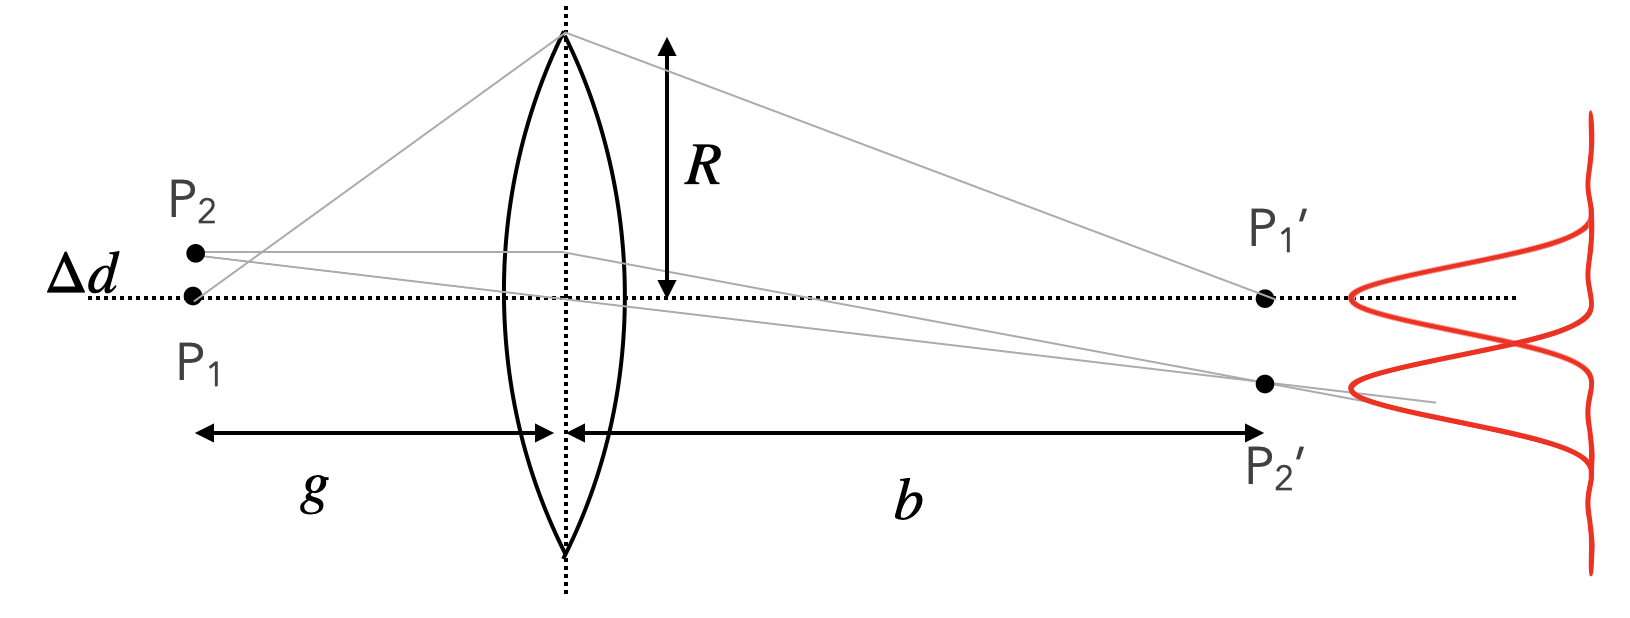
\includegraphics[width=0.8\linewidth,height=\textheight,keepaspectratio]{wave-optics/img/resolution_definition.png}

}

\caption{Illustration showing two point sources and their overlapping
diffraction patterns as they approach each other.}

\end{figure}%

Each point source produces its own diffraction pattern. As the sources
move closer, their patterns begin to overlap, making it harder to
distinguish between them.

\textbf{Rayleigh's Resolution Criterion:}

\begin{itemize}
\tightlist
\item
  Two point sources are considered \textbf{just resolvable} when the
  principal maximum (center) of one Airy pattern coincides with the
  first minimum (dark ring) of the other.
\end{itemize}

\begin{figure}[H]

{\centering 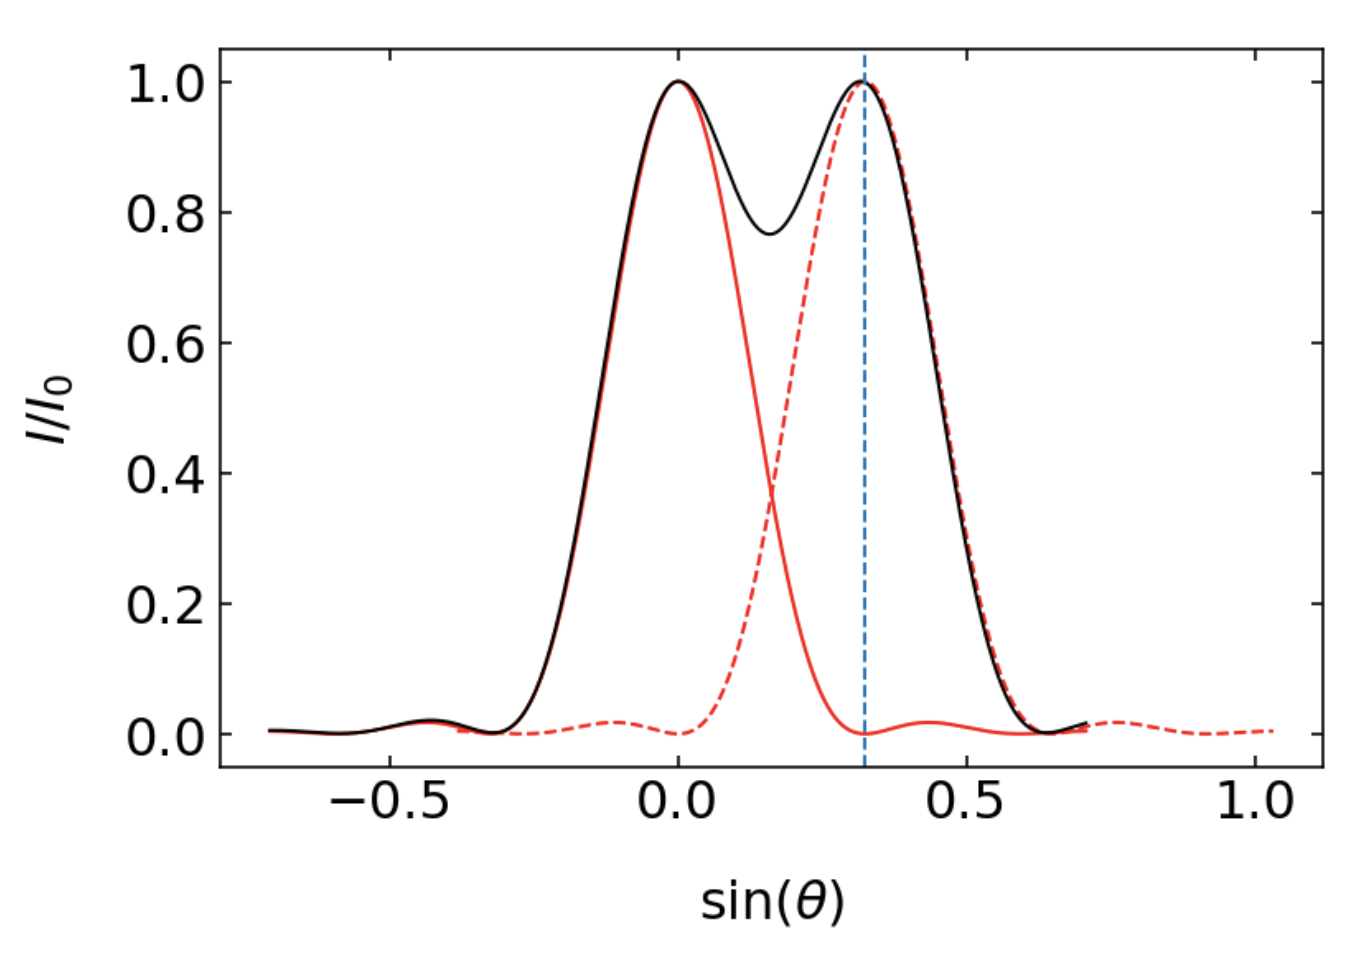
\includegraphics[width=0.5\linewidth,height=\textheight,keepaspectratio]{wave-optics/img/resolution_rayleigh.png}

}

\caption{Graph depicting Rayleigh's criterion, showing the intensity
profiles of two overlapping Airy patterns.}

\end{figure}%

For \textbf{incoherent light sources} (where the light waves are not in
phase), this criterion corresponds to a 26\% dip in intensity between
the two peaks, which is generally sufficient for the human eye or
detectors to distinguish the two sources as separate.

\textbf{Angle to the First Minimum:}

The angle \(\theta_1\) to the first minimum of the diffraction pattern
from a circular aperture of radius \(R\) is given by:

\[
   \sin(\theta_1) = 1.22\, \frac{\lambda}{2R}
   \]

Since the diameter of the aperture \(D = 2R\), this can also be written
as:

\[
   \sin(\theta_1) = 1.22\, \frac{\lambda}{D}
   \]

The factor 1.22 arises from the first zero of the Bessel function
\(J_1\) that describes the diffraction pattern of a circular aperture.

\textbf{Small Angle Approximation:}

For small angles (common in optical systems),
\(\sin(\theta_1) \approx \theta_1\) in radians.

\textbf{Relating Angular to Linear Separation in the Image Plane:}

The angular resolution \(\theta_1\) corresponds to a linear separation
\(\Delta x\) in the image plane (at image distance \(b\)):

\[
   \theta_1 = \frac{\Delta x}{b}
   \]

\textbf{Combining the Equations:}

Substituting \(\theta_1\):

\[
   \frac{\Delta x}{b} = 1.22\, \frac{\lambda}{D}
   \]

Solving for \(\Delta x\):

\[
   \Delta x = 1.22\, \frac{\lambda b}{D}
   \]

\textbf{Considering the Object Plane:}

The magnification \(M\) of the optical system is:

\[
   M = \frac{b}{g}
   \]

where \(g\) is the object distance. The corresponding separation in the
object plane (\(\Delta d\)) is:

\[
   \Delta d = \frac{\Delta x}{M} = \frac{\Delta x \, g}{b}
   \]

Substituting \(\Delta x\):

\[
   \Delta d = 1.22\, \frac{\lambda b}{D} \times \frac{g}{b} = 1.22\, \frac{\lambda g}{D}
   \]

\textbf{Introducing Numerical Aperture (NA):}

The \textbf{numerical aperture} (NA) of the lens is defined as:

\[
   \text{NA} = n \sin(\alpha)
   \]

where:

\begin{itemize}
\tightlist
\item
  \(n\) is the refractive index of the medium between the object and the
  lens.
\item
  \(\alpha\) is the half-angle of the maximum cone of light that can
  enter or exit the lens.
\end{itemize}

Since \(\sin(\alpha) = \frac{R}{g}\), we have:

\[
   D = 2R = 2 g \sin(\alpha)
   \]

Substituting \(D\) into \(\Delta d\):

\[
   \Delta d = 1.22\, \frac{\lambda g}{2 g \sin(\alpha)} = \frac{1.22\, \lambda}{2 \sin(\alpha)} = \frac{0.61\, \lambda}{\sin(\alpha)}
   \]

Therefore, incorporating the refractive index \(n\):

\[
   \Delta d = \frac{0.61\, \lambda}{n \sin(\alpha)} = \frac{0.61\, \lambda}{\text{NA}}
   \]

Under Rayleigh's resolution criterion, several key factors influence the
resolving power of an optical system.

Firstly, a \textbf{higher numerical aperture (NA)} improves resolution.
This increase can be achieved by enhancing either the refractive index
\(n\) of the medium between the object and the lens or the sine of the
collection angle \(\sin(\alpha)\). Since the NA is defined as
\(\text{NA} = n \sin(\alpha)\), a larger NA allows the lens to gather
more diffracted light, thereby resolving finer details in the image. In
air, where the refractive index is approximately \(n \approx 1\), the
\textbf{maximum achievable NA is less than 1}, which limits the
resolution. This limitation arises because the maximum value of
\(\sin(\alpha)\) is 1 (when \(\alpha = 90^\circ\)), so the NA in air
cannot exceed 1. In practical systems, the collection angle \(\alpha\)
is much less than \(90^\circ\), further reducing the NA and thus the
resolution. Immersion lenses, which use a medium with a higher
refractive index (such as water or oil), can achieve higher NAs,
overcoming this limitation and improving resolution.

Secondly, using \textbf{shorter wavelengths} \((\lambda)\) of light
leads to better resolution. According to the formula
\(\Delta d = \frac{0.61\, \lambda}{\text{NA}}\), the minimum resolvable
distance \(\Delta d\) is directly proportional to the wavelength.
Therefore, decreasing the wavelength reduces \(\Delta d\), allowing the
optical system to distinguish smaller features of the object.

\begin{tcolorbox}[enhanced jigsaw, breakable, toptitle=1mm, bottomrule=.15mm, colbacktitle=quarto-callout-note-color!10!white, title=\textcolor{quarto-callout-note-color}{\faInfo}\hspace{0.5em}{Note}, arc=.35mm, rightrule=.15mm, bottomtitle=1mm, opacityback=0, toprule=.15mm, coltitle=black, leftrule=.75mm, opacitybacktitle=0.6, colback=white, left=2mm, titlerule=0mm, colframe=quarto-callout-note-color-frame]

\textbf{Rayleigh's Resolution Criterion}

Two incoherent point sources can be resolved when their minimum
separation \(\Delta d\) satisfies:

\[
\Delta d \geq \frac{0.61\, \lambda}{\text{NA}}
\]

\textbf{Where:}

\begin{itemize}
\tightlist
\item
  \(\Delta d\) is the minimum resolvable distance between the two point
  sources.
\item
  \(\lambda\) is the wavelength of the light used for imaging.
\item
  \(\text{NA} = n \sin(\alpha)\) is the numerical aperture of the
  optical system.

  \begin{itemize}
  \tightlist
  \item
    \(n\) is the refractive index of the medium.
  \item
    \(\alpha\) is the half-angle of the maximum cone of light entering
    the lens.
  \end{itemize}
\end{itemize}

\end{tcolorbox}

\subsection{Abbe's Criterion for
Resolution}\label{abbes-criterion-for-resolution}

\textbf{Limitations of Rayleigh's Criterion:}

\begin{itemize}
\tightlist
\item
  Rayleigh's criterion applies to \textbf{incoherent} light sources,
  where the intensities of the diffraction patterns add directly.
\item
  It does not fully account for the effects of coherence and
  interference in the imaging process.
\end{itemize}

\textbf{Ernst Abbe} developed a theory that considers the imaging of
\textbf{coherent} light sources, where the phases of the waves are
correlated. It emphasizes the importance of diffracted orders and
spatial frequencies in the formation of images.

The key concepts in Abbe's theory are

\textbf{Diffraction Grating Analogy:}

\begin{itemize}
\tightlist
\item
  An object with fine details can be thought of as a diffraction grating
  that scatters light into multiple diffraction orders.
\item
  The ability to resolve these fine details depends on the optical
  system's capacity to capture these diffracted orders.
\end{itemize}

\textbf{Spatial Frequencies:}

\begin{itemize}
\tightlist
\item
  The finer the details in the object, the higher the spatial frequency.
\item
  High spatial frequencies correspond to larger angles in the
  diffraction pattern.
\end{itemize}

\textbf{Optical Transfer Function:}

\begin{itemize}
\tightlist
\item
  Describes how different spatial frequencies are transmitted through
  the optical system.
\item
  An optical system with a larger NA can transmit higher spatial
  frequencies, improving resolution.
\end{itemize}

Following that analogy, Abbe's criterion states that the minimum
resolvable distance \(\Delta d\) between two points in the object plane
is given by:

\[
\Delta d = \frac{\lambda}{2 \text{NA}}
\]

\begin{tcolorbox}[enhanced jigsaw, breakable, toptitle=1mm, bottomrule=.15mm, colbacktitle=quarto-callout-note-color!10!white, title=\textcolor{quarto-callout-note-color}{\faInfo}\hspace{0.5em}{Rayleigh's and Abbe's criteria}, arc=.35mm, rightrule=.15mm, bottomtitle=1mm, opacityback=0, toprule=.15mm, coltitle=black, leftrule=.75mm, opacitybacktitle=0.6, colback=white, left=2mm, titlerule=0mm, colframe=quarto-callout-note-color-frame]

\begin{itemize}
\item
  \textbf{Abbe's Limit:}

  \begin{itemize}
  \tightlist
  \item
    \(\Delta d = \frac{\lambda}{2 \text{NA}}\)
  \item
    Emphasizes coherent imaging and the transmission of at least two
    diffracted orders (zeroth and first) for resolution.
  \end{itemize}
\item
  \textbf{Rayleigh's Limit:}

  \begin{itemize}
  \tightlist
  \item
    \(\Delta d = \frac{0.61\, \lambda}{\text{NA}}\)
  \item
    Based on the visibility of intensity dips in the overlapping Airy
    patterns of incoherent sources.
  \end{itemize}
\end{itemize}

\textbf{Implications in Microscopy:}

Coherent Illumination:

\begin{itemize}
\tightlist
\item
  Techniques like phase-contrast or interference microscopy rely on
  coherent light.
\item
  Abbe's criterion is more appropriate for these methods.
\end{itemize}

Incoherent Illumination:

\begin{itemize}
\tightlist
\item
  Common in conventional bright-field microscopy.
\item
  Rayleigh's criterion provides a practical resolution limit.
\end{itemize}

Importance of Abbe's Criterion:

\begin{itemize}
\tightlist
\item
  Highlights the role of interference between diffracted waves in image
  formation.
\item
  Demonstrates that resolution is fundamentally limited by the
  wavelength of light and the NA of the system.
\item
  Suggests that capturing higher spatial frequencies (larger NA) leads
  to better resolution.
\end{itemize}

\end{tcolorbox}

\section{Using Huygens Sources for
more}\label{using-huygens-sources-for-more}

The Huygens principle is a powerful tool to calculate the diffraction
pattern of an aperture. The idea is to consider the aperture as a
collection of point sources, which emit spherical waves. The
superposition of all these waves will then give the total wave field.
Below is a Python code which demonstrates the calculation of the
diffraction pattern of a spherical mirror. It uses Huygens sources
placed on an arc (see left). The right image shows the resulting
diffraction pattern in the focal plane of the mirror.

\begin{center}
\pandocbounded{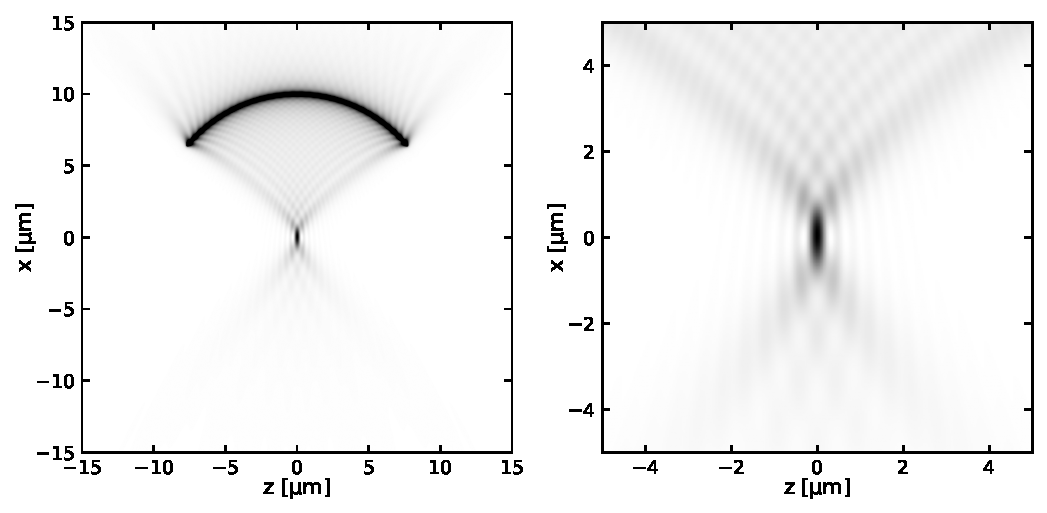
\includegraphics[keepaspectratio]{wave-optics/Diffraction2_files/figure-pdf/cell-3-output-1.pdf}}
\end{center}

The pattern changes with increasing angle of the arc, which is
consistent with our knowledge of the numerical aperature defining the
resolution of and optical system. The changes are especially visible
along the vertical axis.

\begin{center}
\pandocbounded{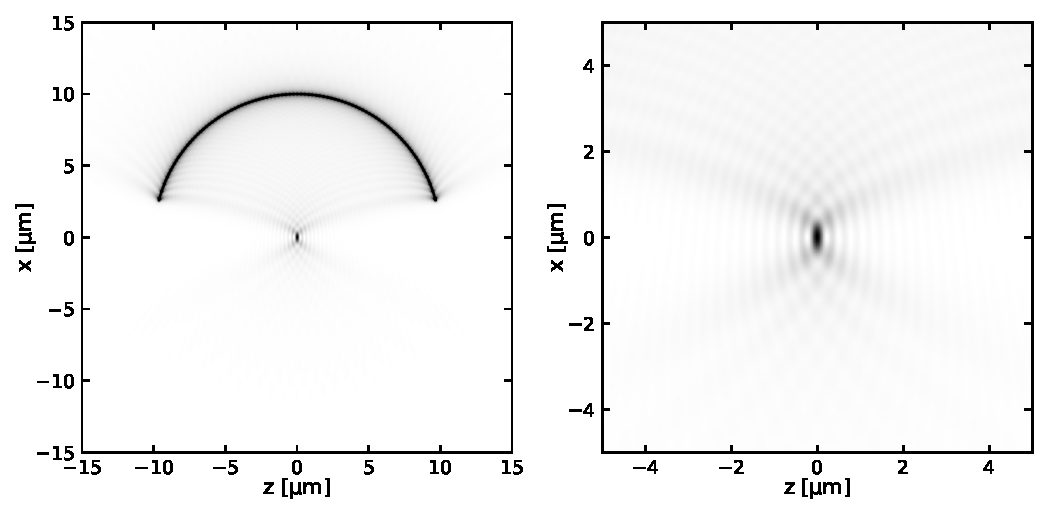
\includegraphics[keepaspectratio]{wave-optics/Diffraction2_files/figure-pdf/cell-4-output-1.pdf}}
\end{center}

\chapter{Fresnel Zones}\label{fresnel-zones}

We want to take a more general look at diffraction by exploring a
concept known as Fresnel zones. Consider spherical waves of wavelength
\(\lambda\) emitted from a source, as indicated by the solid line in the
sketch below.

\begin{figure}[H]

{\centering 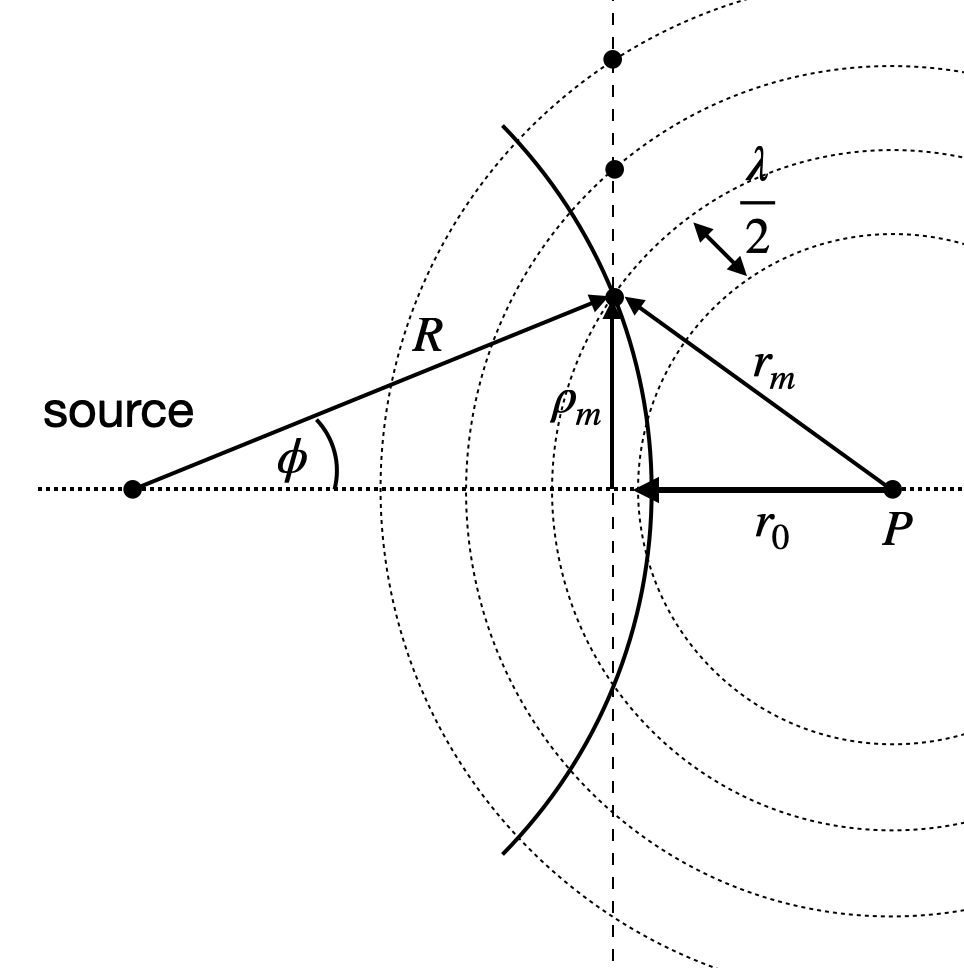
\includegraphics[width=0.65\linewidth,height=\textheight,keepaspectratio]{wave-optics/img/fresnel_zones.png}

}

\caption{Construction of the Fresnel Zones.}

\end{figure}%

We will examine the intensity of the wave at a point \(P\). To do this,
we consider the amplitude contributions from all points on the
wavefront, as each point on the wavefront acts as a Huygens source
contributing to the intensity at point \(P\).

Instead of calculating the intensity explicitly, we will analyze the
distances of individual points on the wavefront from point \(P\).
Specifically, we look at concentric circles around point \(P\), where
the radius of each circle increases by \(\lambda/2\), i.e.,

\[
r_m = r_0 + m \frac{\lambda}{2}
\]

where \(m\) is an integer. The regions between \(r_m\) and \(r_{m+1}\)
are called \textbf{Fresnel zones}. If we consider two neighboring zones,
each zone contains pairs of points that are exactly \(\lambda/2\) out of
phase. This means that these pairs of points would lead to destructive
interference. If we remove these points, we are left with constructive
interference along the optical axis only. We can construct such an
aperture by calculating the ring radius

\[
\rho_{m}^2 = \left( r_0 + m \frac{\lambda}{2} \right)^2 - r_0^2
\]

according to the sketch above. This yields

\[
\rho_m^2 = r_0 m \lambda + m^2 \frac{\lambda^2}{4}
\]

For \(r_{0} \gg \lambda\), we can simplify the above formula to

\[
\rho_m = \sqrt{m r_0 \lambda}
\]

which gives the radius of the individual zones. The width of the zones
is given by

\[
\Delta \rho_m = \rho_{m+1} - \rho_m = \sqrt{r_0 \lambda} (\sqrt{m+1} - \sqrt{m})
\]

\section{Fresnel Zone Plate}\label{fresnel-zone-plate}

If we now fill the ring from \(\rho_m\) to \(\rho_{m+1}\) on a glass
slide but leave the ring from \(\rho_{m+1}\) to \(\rho_{m+2}\)
transparent, we create a so-called \textbf{Fresnel zone plate}. Here,
the radius in the first zone \(r\) ranges from \(r_0\) to
\(r_0 + \lambda/2\). The next zone will range from \(r_0 + \lambda/2\)
to \(r_0 + \lambda\) but is removed from its contribution to the point.

\begin{figure}[H]

{\centering 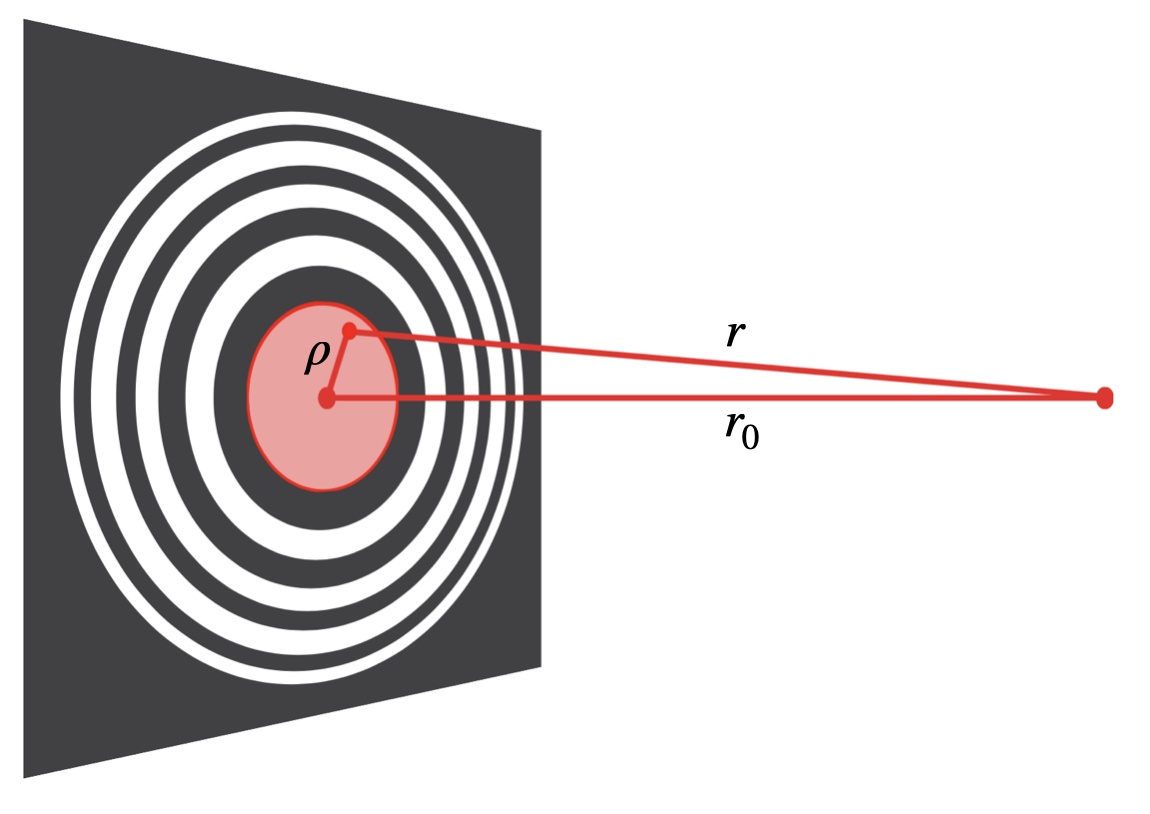
\includegraphics[width=0.75\linewidth,height=\textheight,keepaspectratio]{wave-optics/img/zone_plate.png}

}

\caption{Fresnel zone plate removing destructive interference to the
point on the optical axis.}

\end{figure}%

The Fresnel zone plate can be constructed by defining the inner
reference zone in an arbitrary way. One may either block or transmit the
direct path from the light source along the optical axis, resulting in
either the odd or even zones being transparent.

\begin{figure}[H]

{\centering 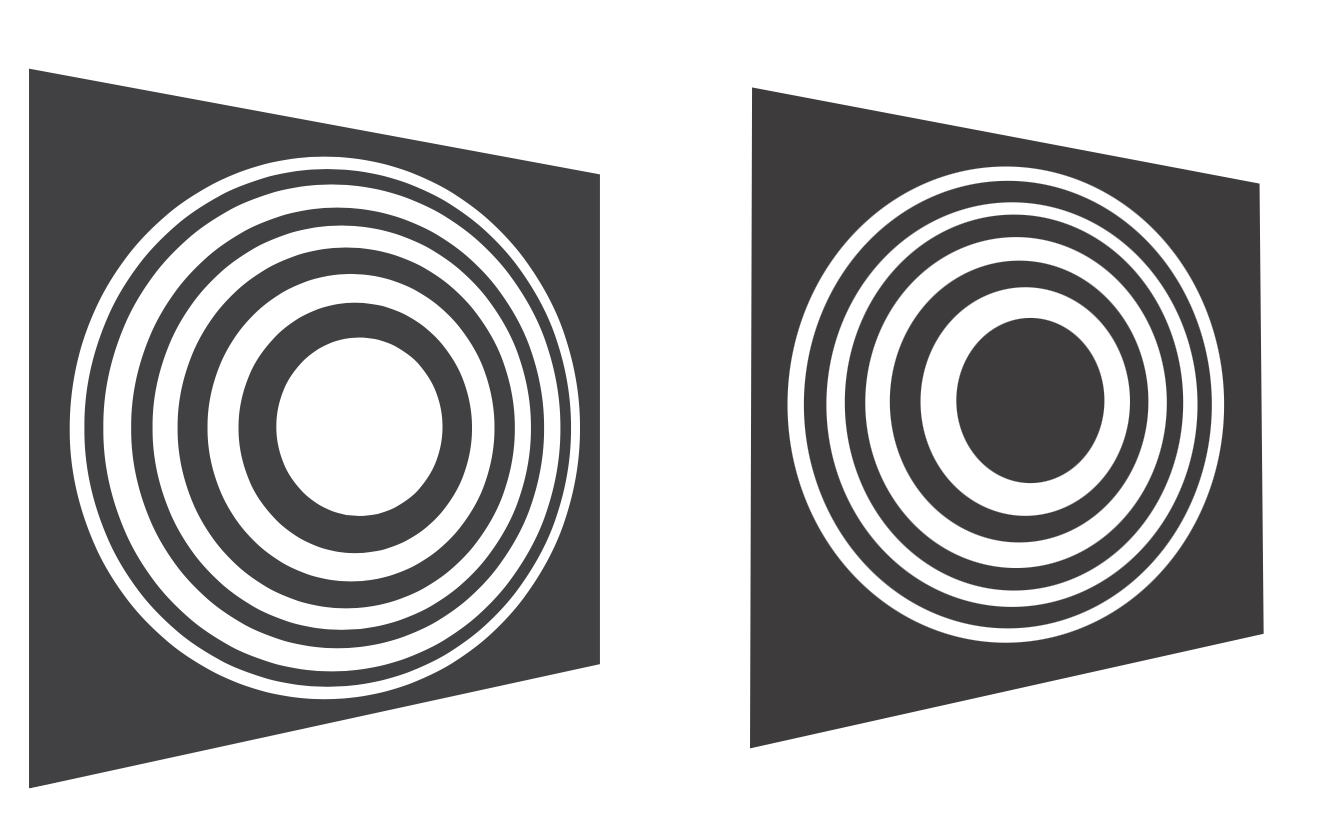
\includegraphics[width=0.9\linewidth,height=\textheight,keepaspectratio]{wave-optics/img/odd_even_zones.png}

}

\caption{Fresnel zone plates with odd (left) or even (right) zones
transparent delivering the same result.}

\end{figure}%

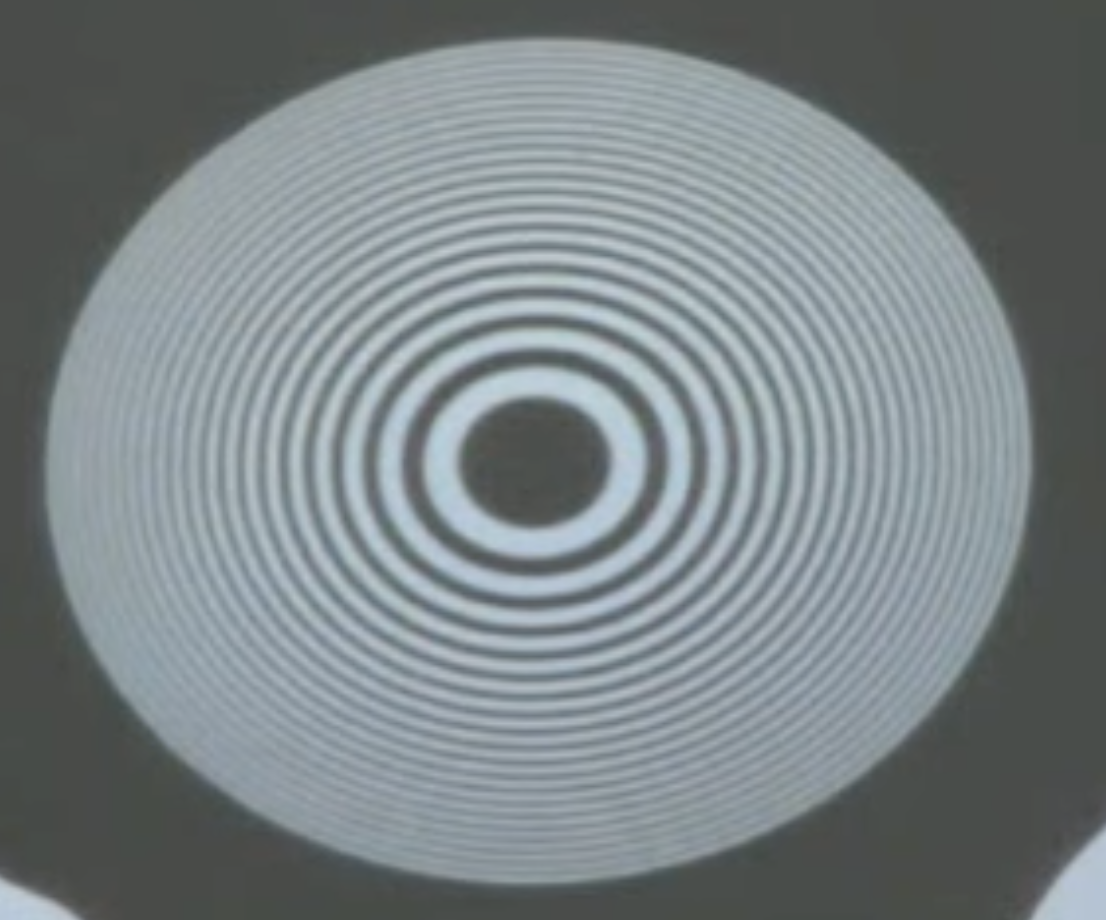
\includegraphics[width=0.49\linewidth,height=\textheight,keepaspectratio]{wave-optics/img/zone_plate_lecture.png}
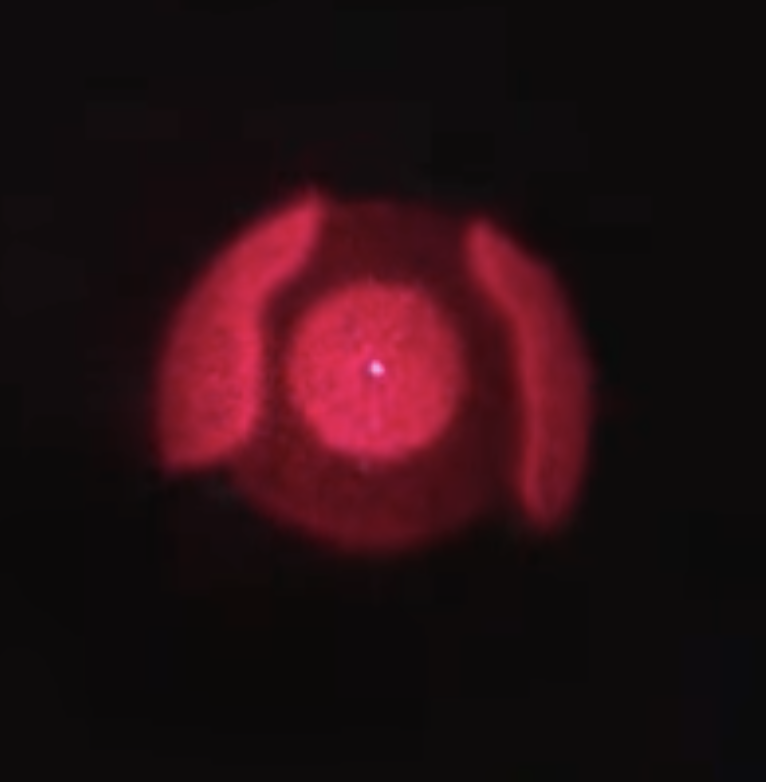
\includegraphics[width=0.4\linewidth,height=\textheight,keepaspectratio]{wave-optics/img/zone_plate_lecture_image.png}

Such zone plates are important for applications where focusing of
radiation is required but the refractive indices are not large enough to
create strong enough refraction. This is especially true for X-ray
radiation.

\begin{figure}[H]

{\centering 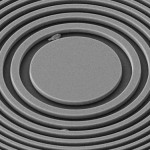
\includegraphics[width=3.125in,height=\textheight,keepaspectratio]{wave-optics/img/zone_plate_xray.jpeg}

}

\caption{Fresnel zone plates for X-ray radiation. Image taken from Ion
beam lithography for Fresnel zone plates in X-ray microscopy - Optics
Express, Vol. 21 Issue 10, pp.11747-11756 (2013).}

\end{figure}%

Below is an calculation of the intensity pattern at the focal distance
of a zone plate from many spherical wave sources if the destructively
interfering waves are not removed (left) and if they are removed.

\begin{figure}[H]

{\centering \pandocbounded{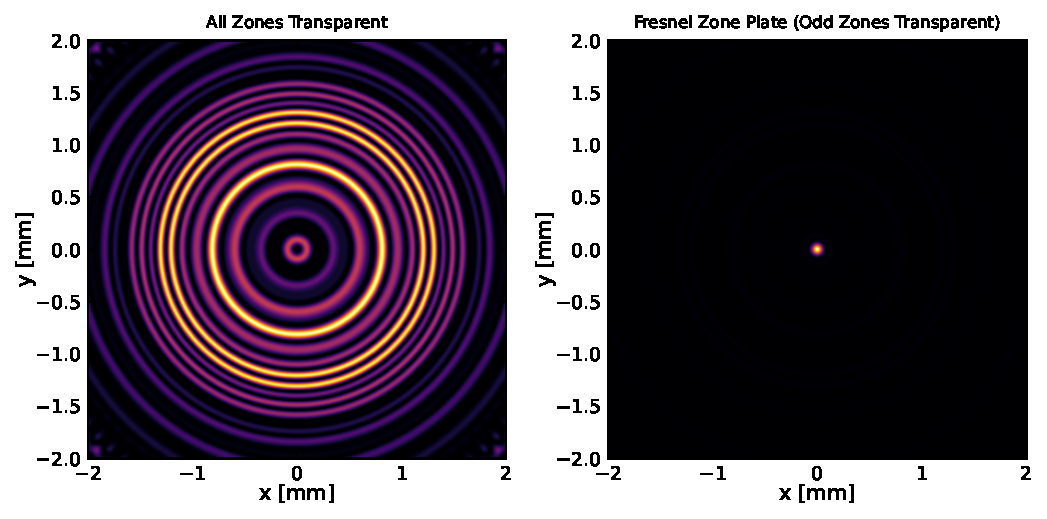
\includegraphics[keepaspectratio]{wave-optics/Fresnel Zones_files/figure-pdf/cell-3-output-1.pdf}}

}

\caption{Consider with care. Need to check the result again.}

\end{figure}%

\section{Applications and Importance of Fresnel Zone
Plates}\label{applications-and-importance-of-fresnel-zone-plates}

Fresnel zone plates are used in various applications, particularly where
traditional lenses are ineffective. Some key applications include:

\textbf{X-ray Microscopy}: Fresnel zone plates are used to focus X-rays,
which have very short wavelengths and require special techniques for
focusing. Traditional lenses are not effective for X-rays due to their
low refractive indices.

\textbf{Optical Systems}: In optical systems, Fresnel zone plates can be
used to create focal points without the need for bulky lenses. This is
particularly useful in compact optical devices.

\textbf{Holography}: Fresnel zone plates are used in holography to
create and reconstruct holograms. They help in manipulating the
wavefronts to produce the desired holographic images.

\textbf{Astronomy}: In astronomy, Fresnel zone plates can be used in
telescopes to focus light from distant stars and galaxies. They offer an
alternative to traditional lenses and mirrors.

\chapter{Diffraction Integral}\label{diffraction-integral}

In the last section about Fresnel zones and the zone plate, we
considered how different paths contribute to the intensity at a point on
the optical axis. We would like to generalize this idea to an integral
formulation that allows us to calculate any kind of diffraction pattern.

\begin{figure}[H]

{\centering 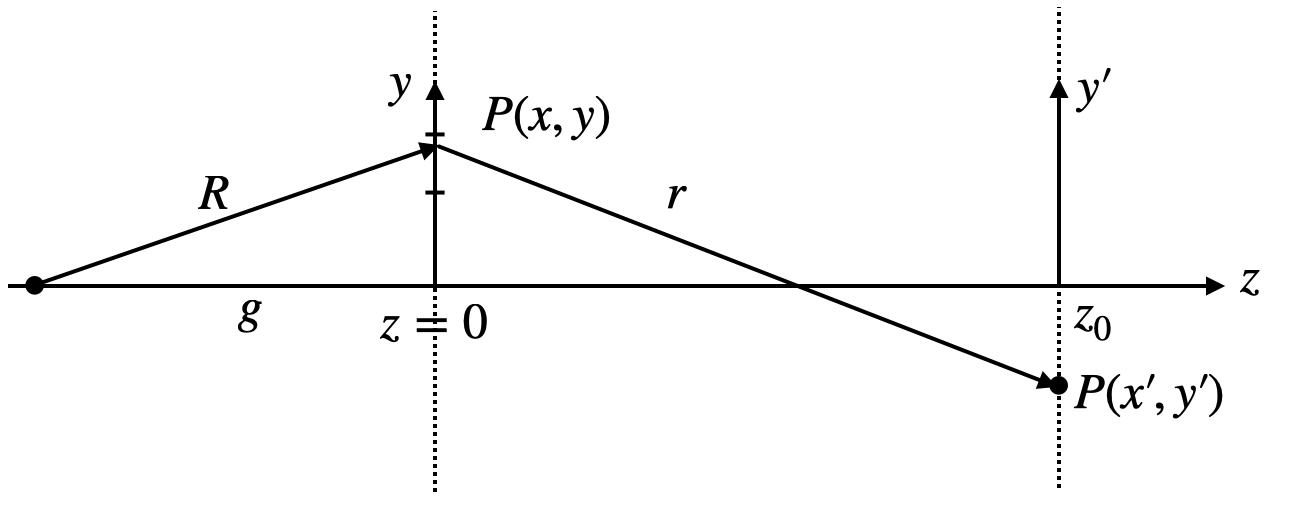
\includegraphics[width=0.8\linewidth,height=\textheight,keepaspectratio]{wave-optics/img/sketch.png}

}

\caption{Diffraction integral.}

\end{figure}%

Assume we have a light source \(S\) as shown in the image above, which
emits a spherical wave (though it does not necessarily have to be a
spherical wave). The spatial amplitude of this wave at the point
\(P(x,y)\) at a tiny aperture element \(d\sigma\) is given by:

\[
U_s(x,y) = U_0(x,y)e^{i\phi(x,y)}
\]

where

\[
U_0 = \frac{A}{R} = \frac{A}{\sqrt{g^2 + x^2 + y^2}}
\]

and

\[
\phi(x,y) = -kR
\]

This represents the amplitude of the Huygens wave, which emanates from
the point \(P(x,y)\) and propagates towards the screen at \(P(x',y')\).
This Huygens wave contributes a fraction of an amplitude \(dU_p\) to the
total amplitude at point \(P(x',y')\), which is given by:

\[
dU_p = C \frac{U_s d\sigma}{r} e^{-ikr}
\]

with \(C = \frac{i \cos(\theta)}{\lambda}\), known as the obliquity
factor, found through a more detailed calculation.

The total amplitude at the point \(P(x',y')\) is then given by the
integral over all contributions:

\[
U_p = \iint C U_s \frac{e^{-ikr}}{r} dx dy
\]

where \(dx dy = d\sigma\). The integral runs over all positions in the
aperture plane \((x,y)\) where there is an opening. This integral is
called the \textbf{Fresnel-Kirchhoff diffraction integral} and allows us
to calculate complex scalar diffraction patterns.

This formulation generalizes the concept of Fresnel zones and provides a
powerful tool for analyzing and predicting diffraction patterns for
various aperture shapes and configurations.

\section{Fresnel Approximation}\label{fresnel-approximation}

The diffraction integral does not always need to be calculated in full;
we can use approximations to obtain diffraction patterns in different
regimes. One such approximation is the \textbf{Fresnel approximation},
which yields the diffraction pattern in the \textbf{near field}.

The distance \(r\) from the point \(P(x,y)\) to the point \(P(x',y')\)
can be written as:

\[
r = \sqrt{z_0^2 + (x - x')^2 + (y - y')^2}
\]

Using a binomial expansion for small angles, we can approximate this as:

\[
r \approx z_0 \left(1 + \frac{(x - x')^2}{2z_0^2} + \frac{(y - y')^2}{2z_0^2} + \ldots \right)
\]

In this approximation, we assume that
\(\cos(\theta) = z_0 / r \approx 1\) and \(C = i / \lambda\),
considering small diffraction angles. Using this approximation, we find
the amplitude of the wave at a point \(P(x',y')\):

\[
U(x', y', z_0) = i \frac{e^{-ikz_0}}{\lambda z_0} \iint U_s(x, y) \exp \left[ -\frac{ik}{2z_0} \left( (x - x')^2 + (y - y')^2 \right) \right] dx dy
\]

As the integration is over \(x\) and \(y\), we can factor out all screen
coordinate elements, yielding:

\[
U(x', y', z_0) = i \frac{e^{-ikz_0}}{\lambda z_0} e^{-\frac{ik}{2z_0}(x'^2 + y'^2)} \iint U_s(x, y) e^{-\frac{ik}{2z_0}(x^2 + y^2)} e^{\frac{ik}{2z_0}(xx' + yy')} dx dy
\]

This is the \textbf{Fresnel approximation}. It simplifies the
calculation of the diffraction pattern in the near field by making
reasonable assumptions about the geometry and angles involved.

\section{Fraunhofer Approximation}\label{fraunhofer-approximation}

If we further assume that the aperture is small as compared to the
distance at which we observe the diffraction pattern, we can further
simplify the Fresnel approximation to yield the Fraunhofer approximation
giving the diffraction patter in the far field. The condition is

\[
z_0\gg\frac{1}{\lambda}(x^2+y^2)
\]

In this case we can neglect the term

\[
e^{ -\frac{ik}{2z_0}(x^2+y^2)} \approx 1
\]

which results in

\[
U(x^{\prime},y^{\prime},z_0)=i\frac{e^{-ikz_0}}{\lambda z_0} e^{-\frac{ik}{2z_0}(x^{\prime 2}+y^{\prime 2})}
\iint U_{s}(x,y)
e^{\frac{ik}{2z_0}(xx^{\prime}+yy^{\prime})} dx dy
\]

\begin{figure}[H]

{\centering 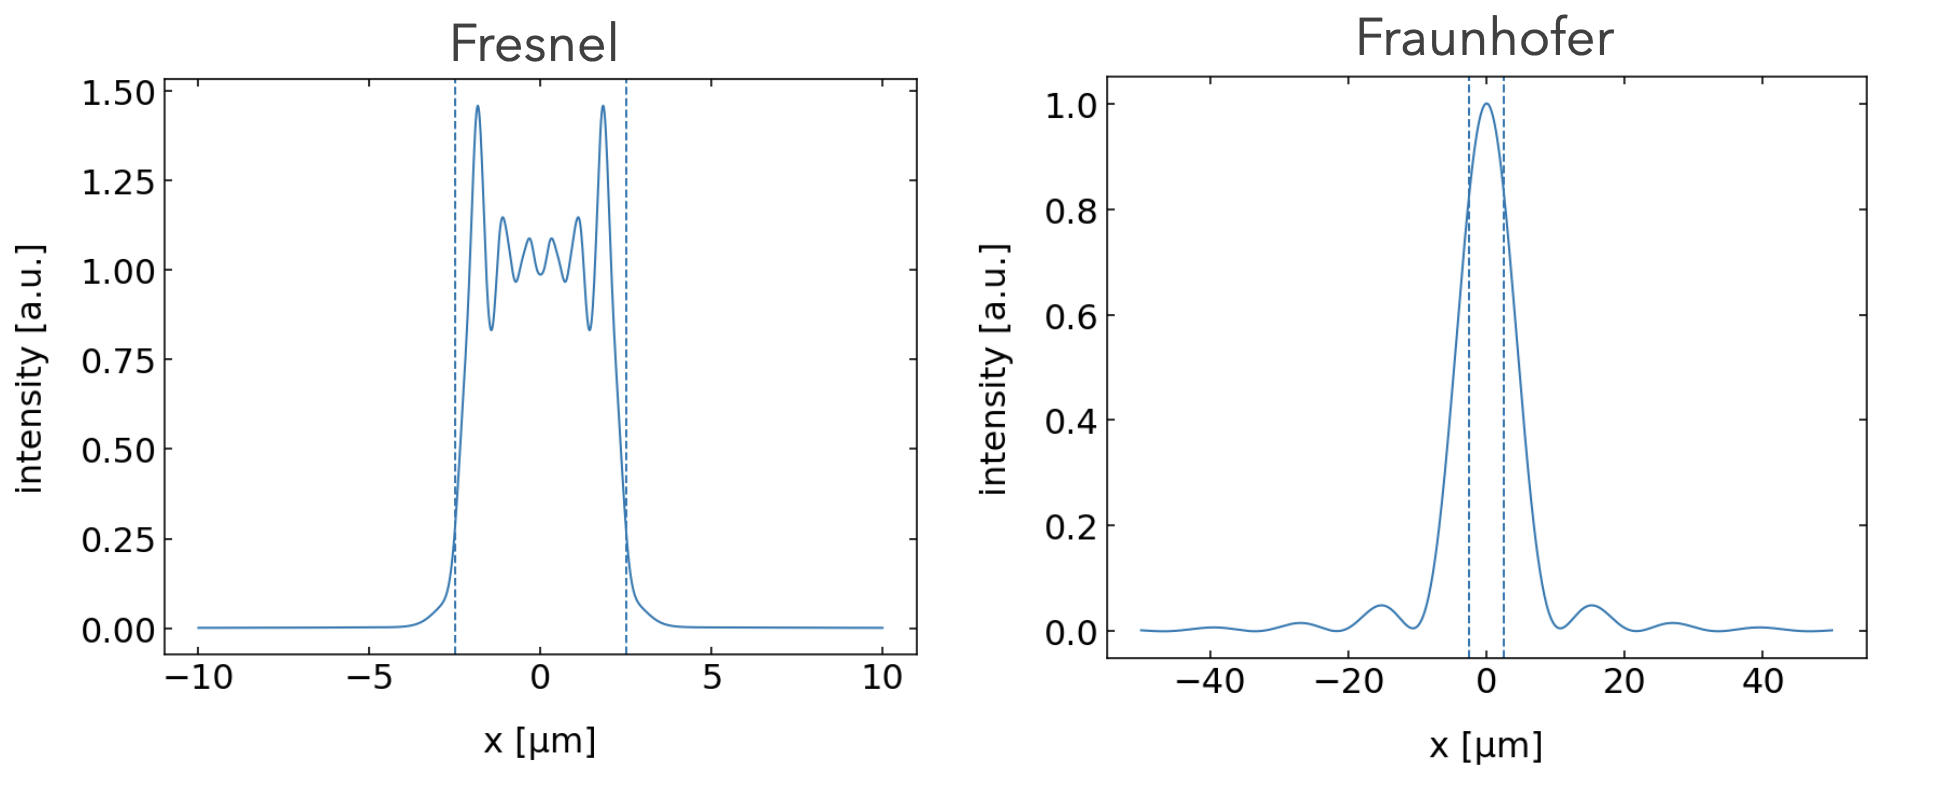
\includegraphics[width=0.9\linewidth,height=\textheight,keepaspectratio]{wave-optics/img/near_far_field.png}

}

\caption{Diffraction pattern of a slit in the near field (Fresnel
diffraction, left) and the far field (Fraunhofer diffraction, right).}

\end{figure}%

While these formulas provide the mathematical tools, we may obtain a
more intuitive idea about the different approximation in the following
way. Consider the image below, where we would like to know about the
diffraction intensity of a slit of width \(b\) at the optical axis at a
distance \(D\).

\begin{figure}[H]

{\centering 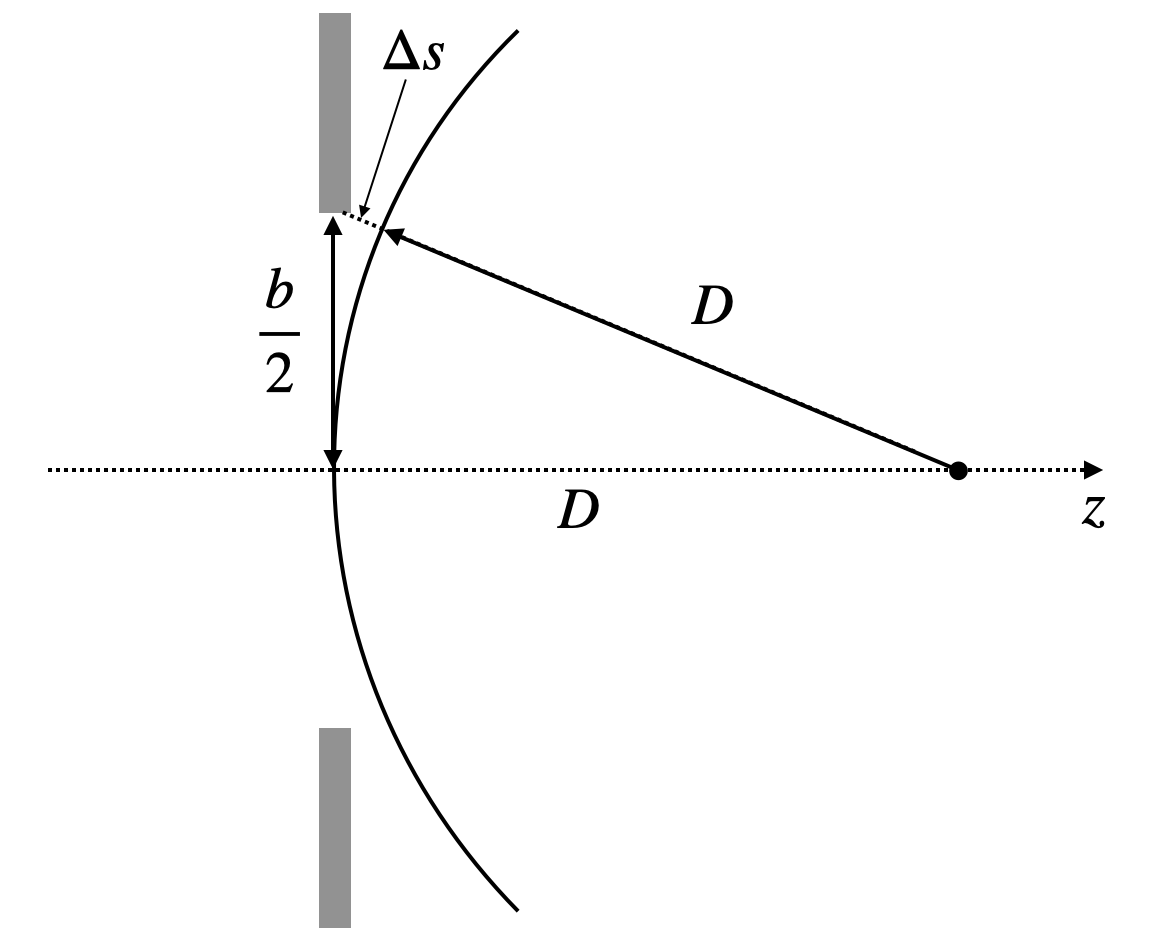
\includegraphics[width=0.55\linewidth,height=\textheight,keepaspectratio]{wave-optics/img/diffraction.png}

}

\caption{Illustration of the importance of additional geometrical path
length difference for the discrimination of Fresnel (near-field) and
Fraunhofer (far-field) diffraction.}

\end{figure}%

The waves from the center of the slit and the edge have to travel
towards that point a different pathlength, whcih we may calculate to

\begin{eqnarray}
\Delta s &=&  \sqrt{\frac{b^2}{4}+D^2}-D\\
&=& D\sqrt{\frac{b^2}{4D^2}+1}-D
\end{eqnarray}

We may develop the square root into a Taylor series and obtain

\begin{eqnarray}
\Delta s &=& \frac{b^2}{8D}-\frac{b^4}{128 D^3}+O(4)\\
&\approx & \frac{b^2}{8D}
\end{eqnarray}

The second order correction term \(\frac{b^2}{8D}\) decreases quadratic
with the distance \(D\) of the point, which means that at large
distances, we can safely assume \(\Delta s=0\) on the axis, i.e.~all
waves arriving at that point have to travel the same distance. This
corresponds to the far-field approximation. To be more specific we
require

\[
\frac{b^2}{8D^2}<\frac{\lambda}{8}
\]

or

\[
\frac{b^2}{\lambda D}<1
\]

to be fullfilled to be in the far field.

\[
F=\frac{b^2}{\lambda D}
\begin{cases}
\ll 1 ,&\textrm{Fraunhofer}\\
\approx 1,& \textrm{Fresnel}\\
\gg 1, & \textrm{Full vector}
\end{cases}
\]

This number \(F\) is called the Frensel number and gives us an idea by
how far the dimensions of the opening contribute to the diffraction
pattern rather than the direction of the wave propagation only.

\section{Babinet's Principle}\label{babinets-principle}

The above considerations of diffraction have some intruiging
consequence. Consider the two apertures in the image below.

\begin{figure}[H]

{\centering 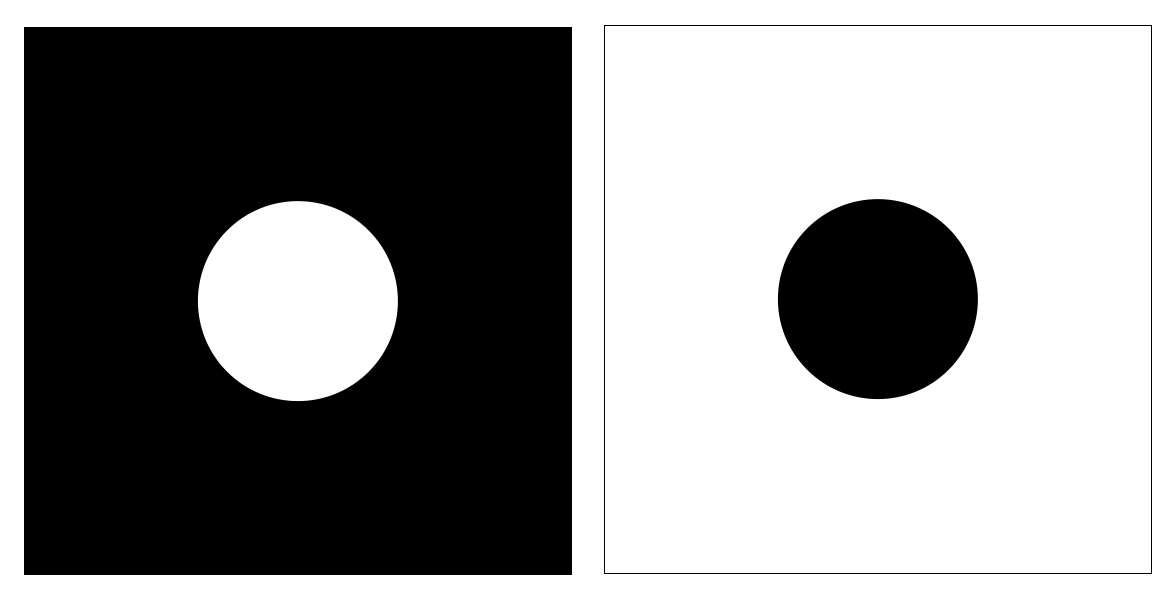
\includegraphics[width=0.6\linewidth,height=\textheight,keepaspectratio]{wave-optics/img/babinet.png}

}

\caption{Two complementary apertures, which have the same diffraction
pattern in the far field.}

\end{figure}%

The left aperture will create in the far field an amplitude distribution
\(U_h\), while the inverse aperture on the right will cause an amplitude
\(U_d\). If we combine both amplitudes in the far field, we obtain a
total amplitude distribution

\[
U=U_h+U_d
\]

In the case when we have two complementary apertures, that total
amplitude has to be zeor, when hole and dot are placed at the same
position. We therefore obtain

\[
U_h=-U_d
\]

and therefore

\[
I_h=I_d
\]

This is the Principle of Babinet which states:

\begin{tcolorbox}[enhanced jigsaw, breakable, toptitle=1mm, bottomrule=.15mm, colbacktitle=quarto-callout-note-color!10!white, title=\textcolor{quarto-callout-note-color}{\faInfo}\hspace{0.5em}{Babinet's Principle}, arc=.35mm, rightrule=.15mm, bottomtitle=1mm, opacityback=0, toprule=.15mm, coltitle=black, leftrule=.75mm, opacitybacktitle=0.6, colback=white, left=2mm, titlerule=0mm, colframe=quarto-callout-note-color-frame]

Babinet's principle states that the far-field diffraction intensity
distribution of complementary apertures is identical. This means that an
opaque object and its complementary aperture (where the object is
replaced by a transparent region and vice versa) produce the same
diffraction pattern in the far field.

\end{tcolorbox}

The images below show an experimental demonstration of Babinet's
principle on a slit and a wire.

\begin{figure}[H]

{\centering 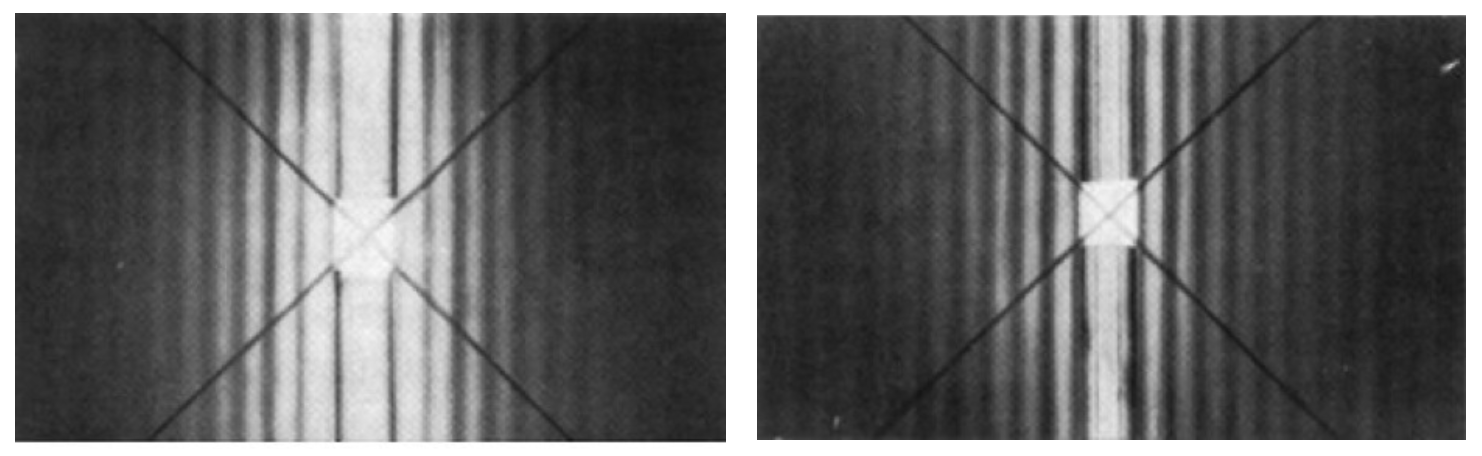
\includegraphics[width=0.9\linewidth,height=\textheight,keepaspectratio]{wave-optics/img/babinet_exp.png}

}

\caption{Babinet's principle demonstrated experimentally on a slit
(left) and a wire (right).}

\end{figure}%


\backmatter


\end{document}
